% !TEX program = xelatex
\documentclass[UTF8,fontset=fandol,a4paper,11pt]{ctexart}
\usepackage[margin=21mm,top=23mm,bottom=22mm,headheight=16pt]{geometry}
\usepackage{amsmath,amssymb,mathtools,bm}
\usepackage{tikz}
\usetikzlibrary{arrows.meta,calc,angles,quotes,patterns}
\usepackage{xcolor,booktabs,array,longtable,enumitem,fancyhdr,needspace}
\usepackage[unicode,hidelinks]{hyperref}
\definecolor{ink}{HTML}{24343C}
\definecolor{accent}{HTML}{166A70}
\definecolor{muted}{HTML}{65747A}
\definecolor{rulegray}{HTML}{D4DDE0}
\definecolor{warm}{HTML}{966037}
\color{ink}
\setlength{\parindent}{2em}
\setlength{\parskip}{4pt}
\linespread{1.12}
\AtBeginDocument{\setlength{\abovedisplayskip}{6pt plus 2pt minus 1pt}
\setlength{\belowdisplayskip}{6pt plus 2pt minus 1pt}
\setlength{\abovedisplayshortskip}{0pt plus 1pt}
\setlength{\belowdisplayshortskip}{4pt plus 1pt}}
\setlist[enumerate]{label=(\arabic*),leftmargin=2.3em,itemsep=3pt,topsep=4pt}
\setlist[itemize]{leftmargin=2em,itemsep=2pt,topsep=4pt}
\allowdisplaybreaks[1]
\setlength{\emergencystretch}{2em}
\setcounter{secnumdepth}{0}
\providecommand{\tightlist}{\setlength{\itemsep}{0pt}\setlength{\parskip}{0pt}}
\ctexset{section={format=\Large\bfseries\color{accent},beforeskip=10pt,afterskip=9pt},
subsection={format=\normalsize\bfseries\color{accent},beforeskip=10pt,afterskip=4pt},
subsubsection={format=\normalsize\bfseries,beforeskip=8pt,afterskip=3pt}}
\pagestyle{fancy}
\fancyhf{}
\fancyhead[L]{\small\color{muted}物理学难题集萃}
% 页眉仅保留书名；版本名称只在封面显示。
\fancyfoot[L]{\small\color{muted}\chapterlabel}
\fancyfoot[R]{\small\thepage}
\renewcommand{\headrulewidth}{0.4pt}
\renewcommand{\footrulewidth}{0pt}
\newcommand{\dd}{\mathop{}\!\mathrm{d}}
\newcommand{\vect}[1]{\bm{#1}}
\newcommand{\tagline}[1]{\noindent{\small\color{muted}#1}\par}
\newcommand{\result}[1]{\begin{equation*}\boxed{#1}\end{equation*}}
\newcommand{\figcaption}[1]{\par\vspace{2pt}{\small\color{muted}#1}\par}
\newcommand{\teach}[2]{\Needspace{4\baselineskip}\subsection*{讲解要点与追问}#1\par\smallskip\noindent\textbf{追问：}#2\par}
\newcommand{\workarea}{\par\vspace{7mm}\noindent{\small\color{muted}作答区}\par\vspace{4mm}
\noindent\textcolor{rulegray}{\rule{\linewidth}{0.3pt}}\par\vspace{16mm}
\noindent\textcolor{rulegray}{\rule{\linewidth}{0.3pt}}\par\vspace{16mm}
\noindent\textcolor{rulegray}{\rule{\linewidth}{0.3pt}}\par\vspace{16mm}
\noindent\textcolor{rulegray}{\rule{\linewidth}{0.3pt}}}
\tikzset{axis/.style={-{Stealth[length=2mm]},thin,color=muted},
motion/.style={-{Stealth[length=2.3mm]},thick,color=accent},
force/.style={-{Stealth[length=2.3mm]},thick,color=warm},
traj/.style={thick,color=accent},guide/.style={dashed,thin,color=muted},
object/.style={thick,color=ink},every node/.style={font=\small}}\widowpenalty=10000\clubpenalty=10000\displaywidowpenalty=10000\newcommand{\chapterlabel}{综合试题（二）}







\hypersetup{pdftitle={综合试题（二）·教师版},pdfauthor={}}

\begin{document}\pdfbookmark[0]{综合试题（二）}{cover}

\thispagestyle{empty}\vspace*{22mm}

\noindent{\Huge\bfseries 物理学难题集萃}\par\vspace{12mm}

\noindent{\LARGE 综合试题（二）}\par\vspace{12mm}

\noindent{\Large\color{accent}教师版}\par\vspace{9mm}

\noindent\textcolor{accent}{\rule{\linewidth}{1pt}}\par\vspace{9mm}

\noindent 第1--6题\par\vfill\clearpage

\pdfbookmark[1]{题目目录}{contents}\section*{题目目录}

\begin{longtable}{@{}r p{113mm} r@{}}\toprule 题号 & 题目 & 页码\\\midrule

\hyperref[q:1]{1} & \hyperref[q:1]{以质点运动研究曲率与正截面} & \pageref{q:1} \\

\hyperref[q:2]{2} & \hyperref[q:2]{弹簧小球与球壳的无碰撞起落} & \pageref{q:2} \\

\hyperref[q:3]{3} & \hyperref[q:3]{以连续折射求最速降线} & \pageref{q:3} \\

\hyperref[q:4]{4} & \hyperref[q:4]{线性引力下的闭合轨道与等效力心} & \pageref{q:4} \\

\hyperref[q:5]{5} & \hyperref[q:5]{采样、空气质量与带电环的三个估算} & \pageref{q:5} \\

\hyperref[q:6]{6} & \hyperref[q:6]{水平磁场中带电圆环由滑动到滚动} & \pageref{q:6} \\

\bottomrule\end{longtable}

\clearpage

\pdfbookmark[2]{第 1 题 以质点运动研究曲率与正截面}{q1}

\section*{第 1 题\quad 以质点运动研究曲率与正截面}\label{q:1}


用物理方法讨论以下几何问题，并与表面张力的压强关系联系。
\begin{enumerate}
\item 平面双曲线为$x^2/A^2-y^2/B^2=1$。设小天体可沿此双曲线的一支在焦点太阳的平方反比引力作用下运动，利用角动量、能量及法向加速度，求右顶点的曲率半径。
\item 一条等距螺旋线绕半径$r$的圆柱轴旋转，每周沿轴方向前进螺距$h$。设计简单的质点运动，求螺旋线各点的曲率半径$\rho$。
\item 圆柱面半径为$r$，$Q$为面上任一点。通过$Q$和该点法线作正截面，选取两对正交正截面，用物理方法证明每对的两条截线在$Q$处都满足相同的$1/\rho_1+1/\rho_2$。说明这与拉普拉斯压强关系$\Delta p=\sigma(1/\rho_1+1/\rho_2)$的一致性；$\sigma$为液体表面张力系数，圆柱取凸面向外的曲率大小。
\end{enumerate}


\begin{center}\begin{minipage}{.98\linewidth}\centering
\begin{tikzpicture}[scale=.8,transform shape]

\draw[axis] (0,0)--(3.5,0) node[right] {$x$};
\draw[axis] (0,-2)--(0,2.2) node[above] {$y$};
\draw[object,domain=-1:1,samples=100] plot ({(exp(\x)+exp(-\x))/2},{1.5*(exp(\x)-exp(-\x))/2});
\fill (1,0) circle (2pt) node[below] {$D$};
\fill (1.803,0) circle (2pt) node[below] {$F$};
\node at (1.5,2.8) {双曲线};
\begin{scope}[xshift=6.3cm]
\draw[object] (-1,-1.5)--(-1,1.5); \draw[object] (1,-1.5)--(1,1.5);
\draw[guide] (0,-1.5) ellipse (1 and .25); \draw[object] (0,1.5) ellipse (1 and .25);
\draw[traj,domain=0:720,samples=250] plot ({cos(\x)},{.25*sin(\x)-1.5+3*\x/720});
\node at (0,2.8) {圆柱螺线与正截面};
\draw[guide] (-1.6,0)--(1.6,0) node[right] {$S_1$};
\draw[guide] (-1,-2)--(-1,2) node[above] {$S_2$};
\fill (-1,0) circle (2pt) node[below left] {$Q$};
\end{scope}

\end{tikzpicture}
\figcaption{图综二.1\quad 双曲线顶点、等距螺线以及圆柱的两类正截面。}
\end{minipage}\end{center}

\Needspace{8\baselineskip}

\pdfbookmark[3]{题型定位}{q1-h0}

\subsection*{题型定位}

借选定质点运动计算曲率，再推导圆柱面正交法曲率和。双曲线用守恒律，螺线用匀速分运动，正截面部分用同切向、同法向和二阶弯曲说明曲率对应。

\Needspace{8\baselineskip}

\pdfbookmark[3]{知识点}{q1-h1}

\subsection*{知识点}

\begin{itemize}
\item 法向加速度与曲率半径，空间曲线的密切平面。
\item 双曲线焦点、渐近线垂距、角动量与机械能。
\item 螺距与速度直角三角形、径向加速度。
\item 圆柱正截线、法曲率的方向依赖及拉普拉斯压强关系。
\end{itemize}

\Needspace{8\baselineskip}

\pdfbookmark[3]{物理图像}{q1-h2}

\subsection*{物理图像}

解图综二.1A标 $D,F$和渐近线垂足，B用一周展开图联系螺距与速度。C在同一切平面内旋转正交方向，D用$s,w$局部截线对照螺线的径向法线；四图分别对应守恒量、加速度、方向和二阶曲率。

\Needspace{8\baselineskip}

\pdfbookmark[3]{解题入口}{q1-h3}

\subsection*{解题入口}

先给出曲率公式所需的两量v和法向a，让学生选择能简化计算的运动。双曲线先用无穷远能量和角动量求出顶点$v$，再代入法向方程。螺线采用圆周与轴向匀速叠加，最后以两方向夹角求曲率和，并用二阶局部式确认正截面对应。

\Needspace{8\baselineskip}

\pdfbookmark[3]{标准解法}{q1-h4}

\subsection*{标准解法}


图综二.1将双曲线、圆柱螺线和正截面分开表示。曲率描述局部轨迹形状，与质点沿轨迹的快慢无关；只要选一种易计算的运动，并求出速率$v$和法向加速度$a_n$，就有$\rho=v^2/a_n$。空间曲线也在该点密切平面内使用这个关系。

求曲率可以先给曲线安排一种容易描述的运动。对同一轨迹，改变运动快慢会同时改变$v^2$与$a_n$，两者之比保持曲线本身的几何长度。平面曲线在一点附近的切线逐渐转动，以曲率圆代替这一小段弯曲，便把转向快慢写成$a_n=v^2/\rho$。若切线两侧的二阶弯曲不同，例如直线与相切圆弧的连接处，则分别取两侧的曲率；本题各条曲线在所讨论点都有确定的二阶形状。对空间曲线，取三个邻近而不共线的点，三点所张平面在相互接近时趋向密切平面，曲率圆位于这个平面内。计算时将加速度分为沿速度的切向部分和垂直速度的法向部分，用法向部分确定曲率。这样的安排将“怎样沿曲线走”与“曲线怎样弯”联系到同一个局部运动图像。

第（1）问，记双曲线焦距$C=\sqrt{A^2+B^2}$，右顶点$D=(A,0)$、右焦点$F=(C,0)$。天体从无穷远沿右支到达$D$再离开，设无穷远速率$v_\infty$，顶点速率$v_D$。顶点切线竖直，故$FD=C-A$与速度垂直。
\begin{center}\begin{minipage}{.98\linewidth}\centering
\begin{tikzpicture}[scale=.85,transform shape]

\draw[axis] (-.2,0)--(4.8,0) node[right] {$x$};
\draw[axis] (0,-2.1)--(0,3.3) node[above] {$y$};
\draw[object,domain=-1:1,samples=120] plot ({exp(\x)+exp(-\x)},{.75*(exp(\x)-exp(-\x))});
\draw[guide] (0,0)--(4.2,3.15) node[above right] {渐近线};
\fill (2,0) circle (2pt) node[below left] {$D(A,0)$};
\fill (2.5,0) circle (2pt) node[below right] {$F(C,0)$};
\coordinate (G) at (1.6,1.2); \fill (G) circle (2pt) node[above left] {$G$};
\draw[guide] (2.5,0)--(G) node[midway,right] {$B$};
\draw[motion] (2,0)--(2,1.2) node[right] {$v_D$};
\draw[motion] (3.3,2.475)--(4.1,3.075) node[midway,above left] {$v_\infty$};
\draw[force] (2,0)--(3.4,0);
\node[right] at (4.5,-1) {顶点引力沿凹侧法线};
\node at (2,-2.8) {$FD=C-A,\quad FG=B$};

\end{tikzpicture}
\figcaption{解图综二.1A\quad 以顶点和无穷远比较角动量、能量，再在D求法向加速度。}
\end{minipage}\end{center}
在图A中，从$F$作到渐近线的垂线，垂足为$G$。远处的一小段运动几乎平行于渐近线，扫过面积是以$v_\infty\dd t$为底、$FG$为高的三角形面积；在$D$处则以$v_D\dd t$为底、$FD$为高。两者给出同一个面积速度，这说明角动量关系使用的是垂直于速度的距离。引力势能在无穷远趋零，在$D$处为负，故小行星接近$D$时动能增大。随后顶点的法向方程只使用此处已经求出的速率与引力。$F$位于$D$右侧，顶点切线竖直，引力沿水平方向指向曲线凹侧，因此顶点的切向加速度为零。将能量与角动量消去引力参数后，所得曲率半径只由$A,B$决定；同一双曲线上的天体质量改变，轨道几何的这个结果保持不变。

解图综二.1A中渐近线为$y=(B/A)x$。焦点到此直线的垂距为
\[
d=\frac{(B/A)C}{\sqrt{1+B^2/A^2}}=B.
\]
远处的速度方向趋于渐近线，因而角动量守恒等价于面积速度守恒：
\[
(C-A)v_D=Bv_\infty,\qquad
v_\infty=\frac{C-A}{B}v_D.
\]
把无穷远的引力势能取零，机械能守恒给
\[
\frac12v_D^2-\frac{GM}{C-A}=\frac12v_\infty^2.
\]
消去$v_\infty$，并用$B^2=(C-A)(C+A)$，
\[
v_D^2\left[1-\frac{(C-A)^2}{B^2}\right]
=\frac{2GM}{C-A},
\qquad
1-\frac{C-A}{C+A}=\frac{2A}{C+A},
\]
故
\[
v_D^2=\frac{GMB^2}{A(C-A)^2}.
\]
在顶点，引力指向$F$，沿曲线凹侧法线，全部提供法向加速度：
\[
\frac{v_D^2}{\rho}=\frac{GM}{(C-A)^2}
\ \Longrightarrow\
\boxed{\rho=\frac{B^2}{A}}.
\]
天体质量和引力参数均被消去，留下双曲线的几何量；所选引力运动只是计算手段，结果只含双曲线的长短尺度。
\begin{center}\begin{minipage}{.98\linewidth}\centering
\begin{tikzpicture}[scale=.8,transform shape]

\draw[object] (-1.2,0)--(-1.2,3); \draw[object] (1.2,0)--(1.2,3);
\draw[guide] (0,0) ellipse (1.2 and .3); \draw[object] (0,3) ellipse (1.2 and .3);
\draw[traj,domain=0:720,samples=300] plot ({1.2*cos(\x)},{.3*sin(\x)+3*\x/720});
\draw[guide] (1.2,0)--(1.7,0) (1.2,1.5)--(1.7,1.5);
\draw[axis,<->] (1.7,0)--(1.7,1.5) node[midway,right] {$h$};
\draw[guide] (0,3)--(1.2,3) node[midway,above] {$r$};
\begin{scope}[xshift=5cm]
\draw[object] (0,0)--(5,0)--(5,.9947184)--cycle;
\draw[guide] (1,0) arc[start angle=0,end angle=11.25173,radius=1];
\node[above] at (1.2,.30) {$\varphi$};
\node[below] at (2.5,0) {$2\pi r$};
\node[right] at (5,.4973592) {$h$};
\node[above] at (3,1.25) {一周展开};
\node at (2,-1.5) {$v^2=v_\perp^2+v_z^2,\quad a_n=v_\perp^2/r$};
\end{scope}

\end{tikzpicture}
\figcaption{解图综二.1B\quad 匀速圆周与轴向平动叠加；展开三角形给切线方向和螺距。}
\end{minipage}\end{center}
图B中一周运动的时间为$2\pi/\omega$，圆周方向通过$2\pi r$，轴向通过$h$，两段距离除以同一个时间就得到两个分速度。展开三角形既给路程比，也给速度比。合速度虽然有轴向分量，轴向匀速运动的加速度为零；全部加速度来自圆周分运动，方向始终沿圆柱法线指向轴线。两个分速度都与该法线垂直，因此总加速度恰为法向加速度。曲率圆心沿此法线位于曲线凹侧，空间螺线每点的局部弯曲由同一组分速度决定。将运动整体移过一段轴向距离或转过一个方位角，只改变点的位置与朝向，两个速度分量的大小保持，所以各点的曲率半径相等。增大螺距时，轴向分速度在同一圆周加速度下增大，合速率平方变大，曲率半径随之增大。

第（2）问，解图综二.1B让质点绕圆柱轴匀速转动，同时沿轴匀速前进。取角速度$\omega$，参数运动为
\[
\boldsymbol r(t)=
\left(r\cos\omega t,\ r\sin\omega t,\ \frac{h\omega t}{2\pi}\right).
\]
圆周分速度$v_\perp=r\omega$，轴向分速度$v_z=h\omega/(2\pi)$，所以
\[
v^2=\omega^2\left[r^2+\left(\frac h{2\pi}\right)^2\right],
\qquad a=\omega^2r.
\]
加速度沿圆柱径向指向轴线，既垂直圆周速度也垂直轴向速度，因此$a=a_n$，不含切向加速度：
\[
\boxed{\rho=\frac{v^2}{a_n}
=r+\frac{h^2}{4\pi^2r}}.
\]
展开一周圆柱面，底边$2\pi r$、高$h$组成直角三角形。若螺线切向与圆周方向夹角为$\varphi$，
\[
\tan\varphi=\frac h{2\pi r},\qquad
\boxed{\rho=\frac r{\cos^2\varphi}}.
\]
结果与点的位置无关；$h=0$退化为圆，螺距增大则轨迹变得更直，曲率半径增大。
\begin{center}\begin{minipage}{.98\linewidth}\centering
\begin{tikzpicture}[scale=.72,transform shape]

\draw[object] (-1.1,-2)--(-1.1,2); \draw[object] (1.1,-2)--(1.1,2);
\draw[object] (0,2) ellipse (1.1 and .3); \draw[guide] (0,-2) ellipse (1.1 and .3);
\draw[guide] (-1.8,0)--(1.8,0) node[right] {$S_1$};
\draw[guide] (-1.1,-2.4)--(-1.1,2.4) node[above] {$S_2$};
\fill (-1.1,0) circle (2pt) node[below left] {$Q$};
\node at (0,-3) {$\rho_1=r,\quad\rho_2=\infty$};
\begin{scope}[xshift=6cm]
\draw[axis] (-2.4,0)--(2.4,0) node[right] {圆周切向};
\draw[axis] (0,-2.4)--(0,2.4) node[above] {轴向};
\draw[traj] (-1.8,-1.2)--(1.8,1.2) node[above right] {$S'_1$切向};
\draw[force] (-1.2,1.8)--(1.2,-1.8) node[below right] {$S'_2$切向};
\draw[guide] (.9,0) arc[start angle=0,end angle=33.69,radius=.9];
\node at (1.15,.35) {$\varphi$};
\fill (0,0) circle (2pt) node[below left] {$Q$};
\node at (0,-3) {两切向正交，所在平面为切平面};
\end{scope}

\end{tikzpicture}
\figcaption{解图综二.1C\quad 圆柱的主正截面与任意旋转的正交正截面方向。}
\end{minipage}\end{center}
正截面通过$Q$及圆柱法线，所以它与切平面的交线确定了曲线在$Q$的切向。图C左侧的两个主方向分别沿圆周、沿轴线；右侧将这两个方向在切平面中转过角$\varphi$，仍构成相互垂直的一对。与圆周方向的夹角增加时，截线中轴向的成分增加，法曲率随$\cos^2\varphi$减小。与之正交的第二条方向正好增加相应的$\sin^2\varphi$部分，两者相加保持$1/r$。圆柱面上的平面斜截线是椭圆，而同切向螺线沿轴向持续前进；两条曲线在远离$Q$的位置有不同形状。这里用同一个径向法线和相同的二阶位移系数来确定局部曲率，比较范围集中在$Q$附近。若$\varphi=0$，第一条截线的曲率为$1/r$、第二条为零；若$\varphi=\pi/4$，两条各分得$1/(2r)$。这两个具体方向把固定的曲率和与各自可变的曲率清楚连接起来。对液面选定一致的内外法线后，拉普拉斯公式使用这两个正截曲率的和，同一点的压强差也因此得到同一个值。

第（3）问，解图综二.1C取第一对正截面：$S_1$垂直轴线，截线是圆；$S_2$包含轴线与$Q$，截线在$Q$附近是直母线，故
\[
\rho_1=r,\quad \rho_2=\infty,\qquad
\frac1{\rho_1}+\frac1{\rho_2}=\frac1r.
\]
第二对正截面在切平面内的交线相互垂直。令第一条切向与圆周方向夹角$\varphi$，第二条夹角$\varphi+\pi/2$。可分别设计同切向的匀速螺线运动；在$Q$处，非直线的螺线加速度沿圆柱法线，切向和法线张成相应正截面。图D下面的二阶位移计算给出螺线与相应正截线在$Q$处相同的曲率大小。直母线方向的曲率为零。由第（2）问，
\[
\frac1{\rho'_1}=\frac{\cos^2\varphi}{r},\qquad
\frac1{\rho'_2}=\frac{\sin^2\varphi}{r}.
\]
所以
\[
\boxed{\frac1{\rho'_1}+\frac1{\rho'_2}=\frac1r
=\frac1{\rho_1}+\frac1{\rho_2}}.
\]
\begin{center}\begin{minipage}{.98\linewidth}\centering
\begin{tikzpicture}[scale=.8,transform shape]

\draw[axis] (-3,0)--(3.4,0) node[right] {$s$切向};
\draw[axis] (0,-.4)--(0,3.5) node[above] {$w$向轴};
\draw[traj,domain=-2.8:2.8,samples=120] plot (\x,{.3*\x*\x});
\fill (0,0) circle (2pt) node[below left] {$Q$};
\draw[guide] (2,0)--(2,1.2)--(0,1.2);
\node[right] at (2,1.2) {$w=s^2\cos^2\varphi/(2r)+O(s^4)$};
\node at (1,-1.5) {正截线与同切向螺线在Q共享二阶曲率};

\end{tikzpicture}
\figcaption{解图综二.1D\quad 正截面局部的切向与法向位移决定二阶曲率。}
\end{minipage}\end{center}
说明同切向螺线与正截线在局部的曲率关系时，解图综二.1D在$Q$附近取正截面坐标：沿切向位移$s$、向轴的法向位移$w$。点的三维坐标可写为
$(r-w,s\cos\varphi,s\sin\varphi)$，代入圆柱方程：
\[
(r-w)^2+s^2\cos^2\varphi=r^2
\ \Longrightarrow\
w=\frac{s^2\cos^2\varphi}{2r}+O(s^4).
\]
局部曲线$s^2/(2\rho')$的二阶系数给出同一个$1/\rho'=\cos^2\varphi/r$，说明比较的是局部曲率圆，所用的是两条曲线在Q附近相同的二阶位移。

对圆柱形液面，两对正截面的曲率和都为$1/r$，拉普拉斯公式因此统一给
\[
\boxed{\Delta p=\frac{\sigma}{r}}.
\]
曲率倒数的和随正截面选择保持不变，正好与同一点压强差不依赖截面选择相符。


\Needspace{8\baselineskip}

\pdfbookmark[3]{关键洞察}{q1-h5}

\subsection*{关键洞察}

曲率是轨迹几何性质，选择运动只是计算工具。圆柱上同一条切向的螺线与平面正截线形状不同，但在Q处共享切向、法向和二阶弯曲；这组局部关系给出两条曲线在$Q$处相同的曲率。

\Needspace{8\baselineskip}

\pdfbookmark[3]{易错点}{q1-h6}

\subsection*{易错点}

\begin{itemize}
\item 将双曲线顶点到焦点距离$C-A$误当曲率半径。
\item 无穷远角动量取$Cv_\infty$而非焦点到渐近线的垂距$B$乘$v_\infty$。
\item 螺线总速度用圆周分速度代替，漏掉轴向分量。
\item 把螺线整体说成平面正截线，未说明局部密切关系。
\item 第二条正交方向仍取同一个$\cos^2\varphi$，曲率和随角度错误变化。
\end{itemize}

\Needspace{8\baselineskip}

\pdfbookmark[3]{课堂讲解建议}{q1-h7}

\subsection*{课堂讲解建议}

可先让学生用几何导数猜双曲线结果，再要求完全用守恒量重算。问为什么两个力学常数最终消失，回答应是曲率只由给定曲线形状决定。螺线部分将一周圆柱面剪开展开，学生在同一三角形上标距离比和速度比。讨论正截面时请他们指出螺线何处不在截面中，再用Q附近的二阶式解释为何仍可借其局部曲率。 追问：“螺距改变时哪一速度分量改变？固定总速率时法向力又怎样变？”让学生用一周展开三角形回答，再联系图V8的分速度平方。关于正截面，学生在$Q$写$w=s^2\cos^2\varphi/(2r)+O(s^4)$，用二阶系数说明局部曲率相同。

\Needspace{8\baselineskip}

\pdfbookmark[3]{变式训练}{q1-h8}

\subsection*{变式训练}

\begin{enumerate}
\item \textbf{等轴双曲线。}取$A=B$，比较顶点曲率半径和顶点到焦点的距离。

由$C=\sqrt{A^2+B^2}$得$C=\sqrt2A$；将$B=A$代入曲率式，
\[\rho=A,\qquad FD=(\sqrt2-1)A,\qquad \rho/FD=\sqrt2+1.\]
图V1的横坐标在$B/A=1$时，实线为1、虚线为$\sqrt2-1$，两条长度对应不同几何对象。顶点引力的大小由$FD$决定，法向加速度的曲率分母则为$\rho$；先用守恒量求出$v_D$，这两个长度才由运动方程相联系。
\begin{center}\begin{minipage}{.98\linewidth}\centering
\begin{tikzpicture}[scale=.88,transform shape]
\draw[axis] (0,0.0000000)--(7.25,0.0000000) node[right] {$B/A$};
\draw[axis] (0.0000000,0)--(0.0000000,2.8);
\node[above left] at (0.0000000,2.8) {$\text{长度}/A$};
\node[below,font=\scriptsize] at (0.0000000,-0.0800000) {$0.25$};
\node[below,font=\scriptsize] at (1.7500000,-0.0800000) {$0.688$};
\node[below,font=\scriptsize] at (3.5000000,-0.0800000) {$1.12$};
\node[below,font=\scriptsize] at (5.2500000,-0.0800000) {$1.56$};
\node[below,font=\scriptsize] at (7.0000000,-0.0800000) {$2$};
\node[left,font=\scriptsize] at (-0.0800000,0.0000000) {$0$};
\node[left,font=\scriptsize] at (-0.0800000,0.8333333) {$1.4$};
\node[left,font=\scriptsize] at (-0.0800000,1.6666667) {$2.8$};
\node[left,font=\scriptsize] at (-0.0800000,2.5000000) {$4.2$};
\draw[thick,color=accent] plot coordinates {(0.0000000,0.0372024) (0.0291667,0.0394042) (0.0583333,0.0416693) (0.0875000,0.0439976) (0.1166667,0.0463893) (0.1458333,0.0488443) (0.1750000,0.0513625) (0.2041667,0.0539441) (0.2333333,0.0565890) (0.2625000,0.0592971) (0.2916667,0.0620686) (0.3208333,0.0649033) (0.3500000,0.0678013) (0.3791667,0.0707627) (0.4083333,0.0737873) (0.4375000,0.0768752) (0.4666667,0.0800265) (0.4958333,0.0832410) (0.5250000,0.0865188) (0.5541667,0.0898599) (0.5833333,0.0932643) (0.6125000,0.0967320) (0.6416667,0.1002630) (0.6708333,0.1038573) (0.7000000,0.1075149) (0.7291667,0.1112358) (0.7583333,0.1150199) (0.7875000,0.1188674) (0.8166667,0.1227782) (0.8458333,0.1267523) (0.8750000,0.1307896) (0.9041667,0.1348903) (0.9333333,0.1390542) (0.9625000,0.1432815) (0.9916667,0.1475720) (1.0208333,0.1519259) (1.0500000,0.1563430) (1.0791667,0.1608234) (1.1083333,0.1653672) (1.1375000,0.1699742) (1.1666667,0.1746445) (1.1958333,0.1793781) (1.2250000,0.1841750) (1.2541667,0.1890352) (1.2833333,0.1939587) (1.3125000,0.1989455) (1.3416667,0.2039956) (1.3708333,0.2091090) (1.4000000,0.2142857) (1.4291667,0.2195257) (1.4583333,0.2248290) (1.4875000,0.2301955) (1.5166667,0.2356254) (1.5458333,0.2411186) (1.5750000,0.2466750) (1.6041667,0.2522948) (1.6333333,0.2579778) (1.6625000,0.2637242) (1.6916667,0.2695338) (1.7208333,0.2754068) (1.7500000,0.2813430) (1.7791667,0.2873425) (1.8083333,0.2934054) (1.8375000,0.2995315) (1.8666667,0.3057209) (1.8958333,0.3119736) (1.9250000,0.3182896) (1.9541667,0.3246689) (1.9833333,0.3311115) (2.0125000,0.3376174) (2.0416667,0.3441866) (2.0708333,0.3508191) (2.1000000,0.3575149) (2.1291667,0.3642740) (2.1583333,0.3710963) (2.1875000,0.3779820) (2.2166667,0.3849310) (2.2458333,0.3919432) (2.2750000,0.3990188) (2.3041667,0.4061576) (2.3333333,0.4133598) (2.3625000,0.4206252) (2.3916667,0.4279540) (2.4208333,0.4353460) (2.4500000,0.4428013) (2.4791667,0.4503200) (2.5083333,0.4579019) (2.5375000,0.4655471) (2.5666667,0.4732556) (2.5958333,0.4810274) (2.6250000,0.4888625) (2.6541667,0.4967609) (2.6833333,0.5047226) (2.7125000,0.5127476) (2.7416667,0.5208359) (2.7708333,0.5289875) (2.8000000,0.5372024) (2.8291667,0.5454806) (2.8583333,0.5538220) (2.8875000,0.5622268) (2.9166667,0.5706949) (2.9458333,0.5792262) (2.9750000,0.5878209) (3.0041667,0.5964788) (3.0333333,0.6052001) (3.0625000,0.6139846) (3.0916667,0.6228324) (3.1208333,0.6317436) (3.1500000,0.6407180) (3.1791667,0.6497557) (3.2083333,0.6588568) (3.2375000,0.6680211) (3.2666667,0.6772487) (3.2958333,0.6865396) (3.3250000,0.6958938) (3.3541667,0.7053113) (3.3833333,0.7147921) (3.4125000,0.7243362) (3.4416667,0.7339436) (3.4708333,0.7436142) (3.5000000,0.7533482) (3.5291667,0.7631455) (3.5583333,0.7730061) (3.5875000,0.7829299) (3.6166667,0.7929171) (3.6458333,0.8029675) (3.6750000,0.8130813) (3.7041667,0.8232583) (3.7333333,0.8334987) (3.7625000,0.8438023) (3.7916667,0.8541693) (3.8208333,0.8645995) (3.8500000,0.8750930) (3.8791667,0.8856498) (3.9083333,0.8962699) (3.9375000,0.9069534) (3.9666667,0.9177001) (3.9958333,0.9285101) (4.0250000,0.9393834) (4.0541667,0.9503200) (4.0833333,0.9613199) (4.1125000,0.9723830) (4.1416667,0.9835095) (4.1708333,0.9946993) (4.2000000,1.0059524) (4.2291667,1.0172688) (4.2583333,1.0286484) (4.2875000,1.0400914) (4.3166667,1.0515976) (4.3458333,1.0631672) (4.3750000,1.0748000) (4.4041667,1.0864962) (4.4333333,1.0982556) (4.4625000,1.1100784) (4.4916667,1.1219644) (4.5208333,1.1339137) (4.5500000,1.1459263) (4.5791667,1.1580023) (4.6083333,1.1701415) (4.6375000,1.1823440) (4.6666667,1.1946098) (4.6958333,1.2069389) (4.7250000,1.2193313) (4.7541667,1.2317870) (4.7833333,1.2443060) (4.8125000,1.2568883) (4.8416667,1.2695338) (4.8708333,1.2822427) (4.9000000,1.2950149) (4.9291667,1.3078503) (4.9583333,1.3207491) (4.9875000,1.3337112) (5.0166667,1.3467365) (5.0458333,1.3598252) (5.0750000,1.3729771) (5.1041667,1.3861924) (5.1333333,1.3994709) (5.1625000,1.4128127) (5.1916667,1.4262179) (5.2208333,1.4396863) (5.2500000,1.4532180) (5.2791667,1.4668130) (5.3083333,1.4804713) (5.3375000,1.4941929) (5.3666667,1.5079778) (5.3958333,1.5218260) (5.4250000,1.5357375) (5.4541667,1.5497123) (5.4833333,1.5637504) (5.5125000,1.5778518) (5.5416667,1.5920165) (5.5708333,1.6062444) (5.6000000,1.6205357) (5.6291667,1.6348903) (5.6583333,1.6493081) (5.6875000,1.6637893) (5.7166667,1.6783337) (5.7458333,1.6929415) (5.7750000,1.7076125) (5.8041667,1.7223469) (5.8333333,1.7371445) (5.8625000,1.7520054) (5.8916667,1.7669297) (5.9208333,1.7819172) (5.9500000,1.7969680) (5.9791667,1.8120821) (6.0083333,1.8272595) (6.0375000,1.8425002) (6.0666667,1.8578042) (6.0958333,1.8731715) (6.1250000,1.8886021) (6.1541667,1.9040960) (6.1833333,1.9196532) (6.2125000,1.9352737) (6.2416667,1.9509574) (6.2708333,1.9667045) (6.3000000,1.9825149) (6.3291667,1.9983885) (6.3583333,2.0143255) (6.3875000,2.0303258) (6.4166667,2.0463893) (6.4458333,2.0625161) (6.4750000,2.0787063) (6.5041667,2.0949597) (6.5333333,2.1112765) (6.5625000,2.1276565) (6.5916667,2.1440998) (6.6208333,2.1606064) (6.6500000,2.1771763) (6.6791667,2.1938095) (6.7083333,2.2105061) (6.7375000,2.2272659) (6.7666667,2.2440890) (6.7958333,2.2609753) (6.8250000,2.2779250) (6.8541667,2.2949380) (6.8833333,2.3120143) (6.9125000,2.3291539) (6.9416667,2.3463568) (6.9708333,2.3636229) (7.0000000,2.3809524)};
\draw[thick,color=accent] (7.65,2.4)--(8.1,2.4);\node[right,font=\scriptsize] at (8.15,2.4) {$\rho/A$};
\draw[thick,dashed,color=warm] plot coordinates {(0.0000000,0.0183193) (0.0291667,0.0193864) (0.0583333,0.0204822) (0.0875000,0.0216067) (0.1166667,0.0227595) (0.1458333,0.0239407) (0.1750000,0.0251500) (0.2041667,0.0263872) (0.2333333,0.0276522) (0.2625000,0.0289448) (0.2916667,0.0302649) (0.3208333,0.0316122) (0.3500000,0.0329866) (0.3791667,0.0343880) (0.4083333,0.0358161) (0.4375000,0.0372708) (0.4666667,0.0387518) (0.4958333,0.0402590) (0.5250000,0.0417923) (0.5541667,0.0433513) (0.5833333,0.0449360) (0.6125000,0.0465461) (0.6416667,0.0481815) (0.6708333,0.0498419) (0.7000000,0.0515272) (0.7291667,0.0532372) (0.7583333,0.0549716) (0.7875000,0.0567303) (0.8166667,0.0585131) (0.8458333,0.0603198) (0.8750000,0.0621502) (0.9041667,0.0640041) (0.9333333,0.0658812) (0.9625000,0.0677815) (0.9916667,0.0697047) (1.0208333,0.0716505) (1.0500000,0.0736189) (1.0791667,0.0756096) (1.1083333,0.0776224) (1.1375000,0.0796571) (1.1666667,0.0817135) (1.1958333,0.0837914) (1.2250000,0.0858907) (1.2541667,0.0880110) (1.2833333,0.0901523) (1.3125000,0.0923143) (1.3416667,0.0944969) (1.3708333,0.0966998) (1.4000000,0.0989228) (1.4291667,0.1011658) (1.4583333,0.1034286) (1.4875000,0.1057109) (1.5166667,0.1080127) (1.5458333,0.1103336) (1.5750000,0.1126735) (1.6041667,0.1150322) (1.6333333,0.1174095) (1.6625000,0.1198053) (1.6916667,0.1222194) (1.7208333,0.1246515) (1.7500000,0.1271015) (1.7791667,0.1295692) (1.8083333,0.1320544) (1.8375000,0.1345570) (1.8666667,0.1370768) (1.8958333,0.1396136) (1.9250000,0.1421672) (1.9541667,0.1447374) (1.9833333,0.1473241) (2.0125000,0.1499271) (2.0416667,0.1525462) (2.0708333,0.1551813) (2.1000000,0.1578322) (2.1291667,0.1604987) (2.1583333,0.1631807) (2.1875000,0.1658780) (2.2166667,0.1685904) (2.2458333,0.1713178) (2.2750000,0.1740600) (2.3041667,0.1768169) (2.3333333,0.1795883) (2.3625000,0.1823740) (2.3916667,0.1851739) (2.4208333,0.1879879) (2.4500000,0.1908157) (2.4791667,0.1936573) (2.5083333,0.1965125) (2.5375000,0.1993812) (2.5666667,0.2022631) (2.5958333,0.2051582) (2.6250000,0.2080663) (2.6541667,0.2109873) (2.6833333,0.2139211) (2.7125000,0.2168674) (2.7416667,0.2198262) (2.7708333,0.2227973) (2.8000000,0.2257806) (2.8291667,0.2287760) (2.8583333,0.2317833) (2.8875000,0.2348024) (2.9166667,0.2378332) (2.9458333,0.2408755) (2.9750000,0.2439292) (3.0041667,0.2469942) (3.0333333,0.2500704) (3.0625000,0.2531577) (3.0916667,0.2562559) (3.1208333,0.2593649) (3.1500000,0.2624846) (3.1791667,0.2656148) (3.2083333,0.2687556) (3.2375000,0.2719066) (3.2666667,0.2750679) (3.2958333,0.2782394) (3.3250000,0.2814208) (3.3541667,0.2846122) (3.3833333,0.2878134) (3.4125000,0.2910242) (3.4416667,0.2942447) (3.4708333,0.2974746) (3.5000000,0.3007139) (3.5291667,0.3039625) (3.5583333,0.3072202) (3.5875000,0.3104871) (3.6166667,0.3137629) (3.6458333,0.3170476) (3.6750000,0.3203411) (3.7041667,0.3236434) (3.7333333,0.3269542) (3.7625000,0.3302735) (3.7916667,0.3336012) (3.8208333,0.3369373) (3.8500000,0.3402816) (3.8791667,0.3436341) (3.9083333,0.3469946) (3.9375000,0.3503631) (3.9666667,0.3537395) (3.9958333,0.3571237) (4.0250000,0.3605156) (4.0541667,0.3639152) (4.0833333,0.3673223) (4.1125000,0.3707370) (4.1416667,0.3741590) (4.1708333,0.3775884) (4.2000000,0.3810250) (4.2291667,0.3844688) (4.2583333,0.3879196) (4.2875000,0.3913775) (4.3166667,0.3948424) (4.3458333,0.3983141) (4.3750000,0.4017927) (4.4041667,0.4052779) (4.4333333,0.4087699) (4.4625000,0.4122684) (4.4916667,0.4157734) (4.5208333,0.4192850) (4.5500000,0.4228029) (4.5791667,0.4263271) (4.6083333,0.4298576) (4.6375000,0.4333943) (4.6666667,0.4369371) (4.6958333,0.4404860) (4.7250000,0.4440409) (4.7541667,0.4476017) (4.7833333,0.4511685) (4.8125000,0.4547410) (4.8416667,0.4583194) (4.8708333,0.4619034) (4.9000000,0.4654931) (4.9291667,0.4690883) (4.9583333,0.4726891) (4.9875000,0.4762954) (5.0166667,0.4799071) (5.0458333,0.4835242) (5.0750000,0.4871466) (5.1041667,0.4907743) (5.1333333,0.4944072) (5.1625000,0.4980452) (5.1916667,0.5016883) (5.2208333,0.5053365) (5.2500000,0.5089897) (5.2791667,0.5126479) (5.3083333,0.5163110) (5.3375000,0.5199789) (5.3666667,0.5236516) (5.3958333,0.5273292) (5.4250000,0.5310114) (5.4541667,0.5346983) (5.4833333,0.5383898) (5.5125000,0.5420859) (5.5416667,0.5457866) (5.5708333,0.5494917) (5.6000000,0.5532013) (5.6291667,0.5569153) (5.6583333,0.5606336) (5.6875000,0.5643563) (5.7166667,0.5680833) (5.7458333,0.5718145) (5.7750000,0.5755499) (5.8041667,0.5792894) (5.8333333,0.5830331) (5.8625000,0.5867808) (5.8916667,0.5905326) (5.9208333,0.5942884) (5.9500000,0.5980482) (5.9791667,0.6018119) (6.0083333,0.6055795) (6.0375000,0.6093509) (6.0666667,0.6131262) (6.0958333,0.6169052) (6.1250000,0.6206880) (6.1541667,0.6244745) (6.1833333,0.6282647) (6.2125000,0.6320585) (6.2416667,0.6358560) (6.2708333,0.6396570) (6.3000000,0.6434615) (6.3291667,0.6472696) (6.3583333,0.6510812) (6.3875000,0.6548961) (6.4166667,0.6587146) (6.4458333,0.6625364) (6.4750000,0.6663615) (6.5041667,0.6701900) (6.5333333,0.6740218) (6.5625000,0.6778568) (6.5916667,0.6816951) (6.6208333,0.6855365) (6.6500000,0.6893812) (6.6791667,0.6932290) (6.7083333,0.6970799) (6.7375000,0.7009339) (6.7666667,0.7047910) (6.7958333,0.7086511) (6.8250000,0.7125142) (6.8541667,0.7163803) (6.8833333,0.7202494) (6.9125000,0.7241214) (6.9416667,0.7279963) (6.9708333,0.7318741) (7.0000000,0.7357547)};
\draw[thick,dashed,color=warm] (7.65,1.9)--(8.1,1.9);\node[right,font=\scriptsize] at (8.15,1.9) {$FD/A$};
\end{tikzpicture}
\figcaption{变图综二.1V1\quad 同一双曲线的顶点曲率与焦点距离}
\end{minipage}\end{center}
\item \textbf{螺距加倍。}取$h=2\pi r$，再将螺距增为$4\pi r$，求两种曲率半径。

一周轴向位移与圆周路程之比为$p=h/(2\pi r)$，因此$v_z/v_\perp=p$。用同一径向加速度$a_n=v_\perp^2/r$，
\[\rho/r=1+p^2.\]
图V2在$p=1$时给$\rho=2r$、$\varphi=\pi/4$，在$p=2$时给$\rho=5r$。保持圆周分速度$v_\perp$时，螺距加倍使轴向速度平方增至四倍，所以曲率半径由2倍半径增为5倍半径。
\begin{center}\begin{minipage}{.98\linewidth}\centering
\begin{tikzpicture}[scale=.88,transform shape]
\draw[axis] (0,0.0000000)--(7.25,0.0000000) node[right] {$p=h/(2\pi r)$};
\draw[axis] (0.0000000,0)--(0.0000000,2.8);
\node[above left] at (0.0000000,2.8) {$\rho/r$};
\node[below,font=\scriptsize] at (0.0000000,-0.0800000) {$0$};
\node[below,font=\scriptsize] at (1.7500000,-0.0800000) {$0.5$};
\node[below,font=\scriptsize] at (3.5000000,-0.0800000) {$1$};
\node[below,font=\scriptsize] at (5.2500000,-0.0800000) {$1.5$};
\node[below,font=\scriptsize] at (7.0000000,-0.0800000) {$2$};
\node[left,font=\scriptsize] at (-0.0800000,0.0000000) {$0$};
\node[left,font=\scriptsize] at (-0.0800000,0.8333333) {$1.73$};
\node[left,font=\scriptsize] at (-0.0800000,1.6666667) {$3.47$};
\node[left,font=\scriptsize] at (-0.0800000,2.5000000) {$5.2$};
\draw[thick,color=accent] plot coordinates {(0.0000000,0.4807692) (0.0291667,0.4808026) (0.0583333,0.4809028) (0.0875000,0.4810697) (0.1166667,0.4813034) (0.1458333,0.4816039) (0.1750000,0.4819712) (0.2041667,0.4824052) (0.2333333,0.4829060) (0.2625000,0.4834736) (0.2916667,0.4841079) (0.3208333,0.4848090) (0.3500000,0.4855769) (0.3791667,0.4864116) (0.4083333,0.4873130) (0.4375000,0.4882812) (0.4666667,0.4893162) (0.4958333,0.4904180) (0.5250000,0.4915865) (0.5541667,0.4928218) (0.5833333,0.4941239) (0.6125000,0.4954928) (0.6416667,0.4969284) (0.6708333,0.4984308) (0.7000000,0.5000000) (0.7291667,0.5016360) (0.7583333,0.5033387) (0.7875000,0.5051082) (0.8166667,0.5069444) (0.8458333,0.5088475) (0.8750000,0.5108173) (0.9041667,0.5128539) (0.9333333,0.5149573) (0.9625000,0.5171274) (0.9916667,0.5193643) (1.0208333,0.5216680) (1.0500000,0.5240385) (1.0791667,0.5264757) (1.1083333,0.5289797) (1.1375000,0.5315505) (1.1666667,0.5341880) (1.1958333,0.5368924) (1.2250000,0.5396635) (1.2541667,0.5425013) (1.2833333,0.5454060) (1.3125000,0.5483774) (1.3416667,0.5514156) (1.3708333,0.5545206) (1.4000000,0.5576923) (1.4291667,0.5609308) (1.4583333,0.5642361) (1.4875000,0.5676082) (1.5166667,0.5710470) (1.5458333,0.5745526) (1.5750000,0.5781250) (1.6041667,0.5817642) (1.6333333,0.5854701) (1.6625000,0.5892428) (1.6916667,0.5930823) (1.7208333,0.5969885) (1.7500000,0.6009615) (1.7791667,0.6050013) (1.8083333,0.6091079) (1.8375000,0.6132812) (1.8666667,0.6175214) (1.8958333,0.6218283) (1.9250000,0.6262019) (1.9541667,0.6306424) (1.9833333,0.6351496) (2.0125000,0.6397236) (2.0416667,0.6443643) (2.0708333,0.6490718) (2.1000000,0.6538462) (2.1291667,0.6586872) (2.1583333,0.6635951) (2.1875000,0.6685697) (2.2166667,0.6736111) (2.2458333,0.6787193) (2.2750000,0.6838942) (2.3041667,0.6891360) (2.3333333,0.6944444) (2.3625000,0.6998197) (2.3916667,0.7052618) (2.4208333,0.7107706) (2.4500000,0.7163462) (2.4791667,0.7219885) (2.5083333,0.7276976) (2.5375000,0.7334736) (2.5666667,0.7393162) (2.5958333,0.7452257) (2.6250000,0.7512019) (2.6541667,0.7572449) (2.6833333,0.7633547) (2.7125000,0.7695312) (2.7416667,0.7757746) (2.7708333,0.7820847) (2.8000000,0.7884615) (2.8291667,0.7949052) (2.8583333,0.8014156) (2.8875000,0.8079928) (2.9166667,0.8146368) (2.9458333,0.8213475) (2.9750000,0.8281250) (3.0041667,0.8349693) (3.0333333,0.8418803) (3.0625000,0.8488582) (3.0916667,0.8559028) (3.1208333,0.8630142) (3.1500000,0.8701923) (3.1791667,0.8774372) (3.2083333,0.8847489) (3.2375000,0.8921274) (3.2666667,0.8995726) (3.2958333,0.9070847) (3.3250000,0.9146635) (3.3541667,0.9223090) (3.3833333,0.9300214) (3.4125000,0.9378005) (3.4416667,0.9456464) (3.4708333,0.9535590) (3.5000000,0.9615385) (3.5291667,0.9695847) (3.5583333,0.9776976) (3.5875000,0.9858774) (3.6166667,0.9941239) (3.6458333,1.0024372) (3.6750000,1.0108173) (3.7041667,1.0192642) (3.7333333,1.0277778) (3.7625000,1.0363582) (3.7916667,1.0450053) (3.8208333,1.0537193) (3.8500000,1.0625000) (3.8791667,1.0713475) (3.9083333,1.0802618) (3.9375000,1.0892428) (3.9666667,1.0982906) (3.9958333,1.1074052) (4.0250000,1.1165865) (4.0541667,1.1258347) (4.0833333,1.1351496) (4.1125000,1.1445312) (4.1416667,1.1539797) (4.1708333,1.1634949) (4.2000000,1.1730769) (4.2291667,1.1827257) (4.2583333,1.1924412) (4.2875000,1.2022236) (4.3166667,1.2120726) (4.3458333,1.2219885) (4.3750000,1.2319712) (4.4041667,1.2420206) (4.4333333,1.2521368) (4.4625000,1.2623197) (4.4916667,1.2725694) (4.5208333,1.2828860) (4.5500000,1.2932692) (4.5791667,1.3037193) (4.6083333,1.3142361) (4.6375000,1.3248197) (4.6666667,1.3354701) (4.6958333,1.3461872) (4.7250000,1.3569712) (4.7541667,1.3678218) (4.7833333,1.3787393) (4.8125000,1.3897236) (4.8416667,1.4007746) (4.8708333,1.4118924) (4.9000000,1.4230769) (4.9291667,1.4343283) (4.9583333,1.4456464) (4.9875000,1.4570312) (5.0166667,1.4684829) (5.0458333,1.4800013) (5.0750000,1.4915865) (5.1041667,1.5032385) (5.1333333,1.5149573) (5.1625000,1.5267428) (5.1916667,1.5385951) (5.2208333,1.5505142) (5.2500000,1.5625000) (5.2791667,1.5745526) (5.3083333,1.5866720) (5.3375000,1.5988582) (5.3666667,1.6111111) (5.3958333,1.6234308) (5.4250000,1.6358173) (5.4541667,1.6482706) (5.4833333,1.6607906) (5.5125000,1.6733774) (5.5416667,1.6860310) (5.5708333,1.6987513) (5.6000000,1.7115385) (5.6291667,1.7243924) (5.6583333,1.7373130) (5.6875000,1.7503005) (5.7166667,1.7633547) (5.7458333,1.7764757) (5.7750000,1.7896635) (5.8041667,1.8029180) (5.8333333,1.8162393) (5.8625000,1.8296274) (5.8916667,1.8430823) (5.9208333,1.8566039) (5.9500000,1.8701923) (5.9791667,1.8838475) (6.0083333,1.8975694) (6.0375000,1.9113582) (6.0666667,1.9252137) (6.0958333,1.9391360) (6.1250000,1.9531250) (6.1541667,1.9671808) (6.1833333,1.9813034) (6.2125000,1.9954928) (6.2416667,2.0097489) (6.2708333,2.0240718) (6.3000000,2.0384615) (6.3291667,2.0529180) (6.3583333,2.0674412) (6.3875000,2.0820312) (6.4166667,2.0966880) (6.4458333,2.1114116) (6.4750000,2.1262019) (6.5041667,2.1410590) (6.5333333,2.1559829) (6.5625000,2.1709736) (6.5916667,2.1860310) (6.6208333,2.2011552) (6.6500000,2.2163462) (6.6791667,2.2316039) (6.7083333,2.2469284) (6.7375000,2.2623197) (6.7666667,2.2777778) (6.7958333,2.2933026) (6.8250000,2.3088942) (6.8541667,2.3245526) (6.8833333,2.3402778) (6.9125000,2.3560697) (6.9416667,2.3719284) (6.9708333,2.3878539) (7.0000000,2.4038462)};
\end{tikzpicture}
\figcaption{变图综二.1V2\quad 螺距通过速度平方改变曲率半径}
\end{minipage}\end{center}
\item \textbf{两正截面转到四十五度。}将圆柱面上一对正交正截面的切向都转到与圆周方向成$45^\circ$的位置，求各自曲率并与主截面比较。

第一条方向满足$\cos^2\varphi=1/2$，正交方向满足$\sin^2\varphi=1/2$，故
\[\rho'_1=\rho'_2=2r,\qquad 1/\rho'_1+1/\rho'_2=1/r.\]
图V3在$\varphi=\pi/4$处两曲线相交，每条纵坐标均为$1/2$；在$\varphi=0$时，则分别为1和0，对应半径$r$的圆和直母线。各自的曲率半径随方向改变，曲率和保持相同。
\begin{center}\begin{minipage}{.98\linewidth}\centering
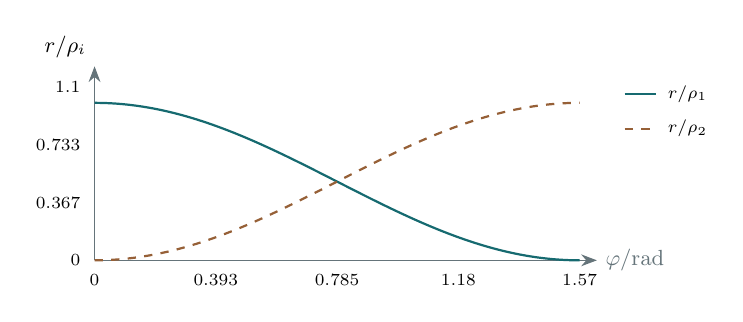
\begin{tikzpicture}[scale=.88,transform shape]
\draw[axis] (0,0.0000000)--(7.25,0.0000000) node[right] {$\varphi/\mathrm{rad}$};
\draw[axis] (0.0000000,0)--(0.0000000,2.8);
\node[above left] at (0.0000000,2.8) {$r/\rho_i$};
\node[below,font=\scriptsize] at (0.0000000,-0.0800000) {$0$};
\node[below,font=\scriptsize] at (1.7500000,-0.0800000) {$0.393$};
\node[below,font=\scriptsize] at (3.5000000,-0.0800000) {$0.785$};
\node[below,font=\scriptsize] at (5.2500000,-0.0800000) {$1.18$};
\node[below,font=\scriptsize] at (7.0000000,-0.0800000) {$1.57$};
\node[left,font=\scriptsize] at (-0.0800000,0.0000000) {$0$};
\node[left,font=\scriptsize] at (-0.0800000,0.8333333) {$0.367$};
\node[left,font=\scriptsize] at (-0.0800000,1.6666667) {$0.733$};
\node[left,font=\scriptsize] at (-0.0800000,2.5000000) {$1.1$};
\draw[thick,color=accent] plot coordinates {(0.0000000,2.2727273) (0.0291667,2.2726299) (0.0583333,2.2723379) (0.0875000,2.2718512) (0.1166667,2.2711699) (0.1458333,2.2702942) (0.1750000,2.2692242) (0.2041667,2.2679601) (0.2333333,2.2665022) (0.2625000,2.2648505) (0.2916667,2.2630055) (0.3208333,2.2609675) (0.3500000,2.2587368) (0.3791667,2.2563137) (0.4083333,2.2536988) (0.4375000,2.2508924) (0.4666667,2.2478950) (0.4958333,2.2447072) (0.5250000,2.2413295) (0.5541667,2.2377624) (0.5833333,2.2340066) (0.6125000,2.2300628) (0.6416667,2.2259315) (0.6708333,2.2216136) (0.7000000,2.2171097) (0.7291667,2.2124206) (0.7583333,2.2075471) (0.7875000,2.2024902) (0.8166667,2.1972505) (0.8458333,2.1918290) (0.8750000,2.1862267) (0.9041667,2.1804446) (0.9333333,2.1744835) (0.9625000,2.1683445) (0.9916667,2.1620287) (1.0208333,2.1555372) (1.0500000,2.1488711) (1.0791667,2.1420314) (1.1083333,2.1350194) (1.1375000,2.1278364) (1.1666667,2.1204834) (1.1958333,2.1129618) (1.2250000,2.1052729) (1.2541667,2.0974180) (1.2833333,2.0893984) (1.3125000,2.0812155) (1.3416667,2.0728707) (1.3708333,2.0643654) (1.4000000,2.0557011) (1.4291667,2.0468793) (1.4583333,2.0379015) (1.4875000,2.0287692) (1.5166667,2.0194840) (1.5458333,2.0100475) (1.5750000,2.0004613) (1.6041667,1.9907271) (1.6333333,1.9808464) (1.6625000,1.9708210) (1.6916667,1.9606527) (1.7208333,1.9503431) (1.7500000,1.9398941) (1.7791667,1.9293073) (1.8083333,1.9185847) (1.8375000,1.9077281) (1.8666667,1.8967393) (1.8958333,1.8856202) (1.9250000,1.8743728) (1.9541667,1.8629989) (1.9833333,1.8515004) (2.0125000,1.8398795) (2.0416667,1.8281380) (2.0708333,1.8162780) (2.1000000,1.8043014) (2.1291667,1.7922104) (2.1583333,1.7800071) (2.1875000,1.7676934) (2.2166667,1.7552716) (2.2458333,1.7427438) (2.2750000,1.7301120) (2.3041667,1.7173785) (2.3333333,1.7045455) (2.3625000,1.6916150) (2.3916667,1.6785895) (2.4208333,1.6654710) (2.4500000,1.6522619) (2.4791667,1.6389644) (2.5083333,1.6255808) (2.5375000,1.6121133) (2.5666667,1.5985644) (2.5958333,1.5849362) (2.6250000,1.5712312) (2.6541667,1.5574516) (2.6833333,1.5435999) (2.7125000,1.5296785) (2.7416667,1.5156896) (2.7708333,1.5016358) (2.8000000,1.4875193) (2.8291667,1.4733427) (2.8583333,1.4591083) (2.8875000,1.4448187) (2.9166667,1.4304762) (2.9458333,1.4160833) (2.9750000,1.4016425) (3.0041667,1.3871562) (3.0333333,1.3726269) (3.0625000,1.3580572) (3.0916667,1.3434495) (3.1208333,1.3288063) (3.1500000,1.3141301) (3.1791667,1.2994234) (3.2083333,1.2846889) (3.2375000,1.2699289) (3.2666667,1.2551460) (3.2958333,1.2403427) (3.3250000,1.2255217) (3.3541667,1.2106854) (3.3833333,1.1958363) (3.4125000,1.1809771) (3.4416667,1.1661102) (3.4708333,1.1512382) (3.5000000,1.1363636) (3.5291667,1.1214891) (3.5583333,1.1066171) (3.5875000,1.0917502) (3.6166667,1.0768910) (3.6458333,1.0620419) (3.6750000,1.0472056) (3.7041667,1.0323845) (3.7333333,1.0175813) (3.7625000,1.0027984) (3.7916667,0.9880384) (3.8208333,0.9733038) (3.8500000,0.9585972) (3.8791667,0.9439210) (3.9083333,0.9292778) (3.9375000,0.9146701) (3.9666667,0.9001004) (3.9958333,0.8855711) (4.0250000,0.8710848) (4.0541667,0.8566440) (4.0833333,0.8422511) (4.1125000,0.8279086) (4.1416667,0.8136189) (4.1708333,0.7993846) (4.2000000,0.7852080) (4.2291667,0.7710915) (4.2583333,0.7570377) (4.2875000,0.7430488) (4.3166667,0.7291273) (4.3458333,0.7152756) (4.3750000,0.7014961) (4.4041667,0.6877911) (4.4333333,0.6741629) (4.4625000,0.6606139) (4.4916667,0.6471465) (4.5208333,0.6337629) (4.5500000,0.6204653) (4.5791667,0.6072562) (4.6083333,0.5941378) (4.6375000,0.5811122) (4.6666667,0.5681818) (4.6958333,0.5553488) (4.7250000,0.5426153) (4.7541667,0.5299835) (4.7833333,0.5174556) (4.8125000,0.5050338) (4.8416667,0.4927202) (4.8708333,0.4805168) (4.9000000,0.4684258) (4.9291667,0.4564493) (4.9583333,0.4445893) (4.9875000,0.4328478) (5.0166667,0.4212268) (5.0458333,0.4097284) (5.0750000,0.3983545) (5.1041667,0.3871070) (5.1333333,0.3759879) (5.1625000,0.3649992) (5.1916667,0.3541425) (5.2208333,0.3434199) (5.2500000,0.3328332) (5.2791667,0.3223842) (5.3083333,0.3120746) (5.3375000,0.3019062) (5.3666667,0.2918809) (5.3958333,0.2820002) (5.4250000,0.2722659) (5.4541667,0.2626797) (5.4833333,0.2532432) (5.5125000,0.2439580) (5.5416667,0.2348257) (5.5708333,0.2258479) (5.6000000,0.2170261) (5.6291667,0.2083619) (5.6583333,0.1998566) (5.6875000,0.1915118) (5.7166667,0.1833289) (5.7458333,0.1753093) (5.7750000,0.1674544) (5.8041667,0.1597654) (5.8333333,0.1522439) (5.8625000,0.1448909) (5.8916667,0.1377078) (5.9208333,0.1306959) (5.9500000,0.1238562) (5.9791667,0.1171901) (6.0083333,0.1106985) (6.0375000,0.1043828) (6.0666667,0.0982438) (6.0958333,0.0922827) (6.1250000,0.0865005) (6.1541667,0.0808982) (6.1833333,0.0754768) (6.2125000,0.0702371) (6.2416667,0.0651801) (6.2708333,0.0603067) (6.3000000,0.0556176) (6.3291667,0.0511137) (6.3583333,0.0467958) (6.3875000,0.0426645) (6.4166667,0.0387207) (6.4458333,0.0349649) (6.4750000,0.0313978) (6.5041667,0.0280201) (6.5333333,0.0248323) (6.5625000,0.0218349) (6.5916667,0.0190285) (6.6208333,0.0164136) (6.6500000,0.0139905) (6.6791667,0.0117598) (6.7083333,0.0097217) (6.7375000,0.0078768) (6.7666667,0.0062251) (6.7958333,0.0047671) (6.8250000,0.0035030) (6.8541667,0.0024330) (6.8833333,0.0015573) (6.9125000,0.0008761) (6.9416667,0.0003894) (6.9708333,0.0000974) (7.0000000,0.0000000)};
\draw[thick,color=accent] (7.65,2.4)--(8.1,2.4);\node[right,font=\scriptsize] at (8.15,2.4) {$r/\rho_1$};
\draw[thick,dashed,color=warm] plot coordinates {(0.0000000,0.0000000) (0.0291667,0.0000974) (0.0583333,0.0003894) (0.0875000,0.0008761) (0.1166667,0.0015573) (0.1458333,0.0024330) (0.1750000,0.0035030) (0.2041667,0.0047671) (0.2333333,0.0062251) (0.2625000,0.0078768) (0.2916667,0.0097217) (0.3208333,0.0117598) (0.3500000,0.0139905) (0.3791667,0.0164136) (0.4083333,0.0190285) (0.4375000,0.0218349) (0.4666667,0.0248323) (0.4958333,0.0280201) (0.5250000,0.0313978) (0.5541667,0.0349649) (0.5833333,0.0387207) (0.6125000,0.0426645) (0.6416667,0.0467958) (0.6708333,0.0511137) (0.7000000,0.0556176) (0.7291667,0.0603067) (0.7583333,0.0651801) (0.7875000,0.0702371) (0.8166667,0.0754768) (0.8458333,0.0808982) (0.8750000,0.0865005) (0.9041667,0.0922827) (0.9333333,0.0982438) (0.9625000,0.1043828) (0.9916667,0.1106985) (1.0208333,0.1171901) (1.0500000,0.1238562) (1.0791667,0.1306959) (1.1083333,0.1377078) (1.1375000,0.1448909) (1.1666667,0.1522439) (1.1958333,0.1597654) (1.2250000,0.1674544) (1.2541667,0.1753093) (1.2833333,0.1833289) (1.3125000,0.1915118) (1.3416667,0.1998566) (1.3708333,0.2083619) (1.4000000,0.2170261) (1.4291667,0.2258479) (1.4583333,0.2348257) (1.4875000,0.2439580) (1.5166667,0.2532432) (1.5458333,0.2626797) (1.5750000,0.2722659) (1.6041667,0.2820002) (1.6333333,0.2918809) (1.6625000,0.3019062) (1.6916667,0.3120746) (1.7208333,0.3223842) (1.7500000,0.3328332) (1.7791667,0.3434199) (1.8083333,0.3541425) (1.8375000,0.3649992) (1.8666667,0.3759879) (1.8958333,0.3871070) (1.9250000,0.3983545) (1.9541667,0.4097284) (1.9833333,0.4212268) (2.0125000,0.4328478) (2.0416667,0.4445893) (2.0708333,0.4564493) (2.1000000,0.4684258) (2.1291667,0.4805168) (2.1583333,0.4927202) (2.1875000,0.5050338) (2.2166667,0.5174556) (2.2458333,0.5299835) (2.2750000,0.5426153) (2.3041667,0.5553488) (2.3333333,0.5681818) (2.3625000,0.5811122) (2.3916667,0.5941378) (2.4208333,0.6072562) (2.4500000,0.6204653) (2.4791667,0.6337629) (2.5083333,0.6471465) (2.5375000,0.6606139) (2.5666667,0.6741629) (2.5958333,0.6877911) (2.6250000,0.7014961) (2.6541667,0.7152756) (2.6833333,0.7291273) (2.7125000,0.7430488) (2.7416667,0.7570377) (2.7708333,0.7710915) (2.8000000,0.7852080) (2.8291667,0.7993846) (2.8583333,0.8136189) (2.8875000,0.8279086) (2.9166667,0.8422511) (2.9458333,0.8566440) (2.9750000,0.8710848) (3.0041667,0.8855711) (3.0333333,0.9001004) (3.0625000,0.9146701) (3.0916667,0.9292778) (3.1208333,0.9439210) (3.1500000,0.9585972) (3.1791667,0.9733038) (3.2083333,0.9880384) (3.2375000,1.0027984) (3.2666667,1.0175813) (3.2958333,1.0323845) (3.3250000,1.0472056) (3.3541667,1.0620419) (3.3833333,1.0768910) (3.4125000,1.0917502) (3.4416667,1.1066171) (3.4708333,1.1214891) (3.5000000,1.1363636) (3.5291667,1.1512382) (3.5583333,1.1661102) (3.5875000,1.1809771) (3.6166667,1.1958363) (3.6458333,1.2106854) (3.6750000,1.2255217) (3.7041667,1.2403427) (3.7333333,1.2551460) (3.7625000,1.2699289) (3.7916667,1.2846889) (3.8208333,1.2994234) (3.8500000,1.3141301) (3.8791667,1.3288063) (3.9083333,1.3434495) (3.9375000,1.3580572) (3.9666667,1.3726269) (3.9958333,1.3871562) (4.0250000,1.4016425) (4.0541667,1.4160833) (4.0833333,1.4304762) (4.1125000,1.4448187) (4.1416667,1.4591083) (4.1708333,1.4733427) (4.2000000,1.4875193) (4.2291667,1.5016358) (4.2583333,1.5156896) (4.2875000,1.5296785) (4.3166667,1.5435999) (4.3458333,1.5574516) (4.3750000,1.5712312) (4.4041667,1.5849362) (4.4333333,1.5985644) (4.4625000,1.6121133) (4.4916667,1.6255808) (4.5208333,1.6389644) (4.5500000,1.6522619) (4.5791667,1.6654710) (4.6083333,1.6785895) (4.6375000,1.6916150) (4.6666667,1.7045455) (4.6958333,1.7173785) (4.7250000,1.7301120) (4.7541667,1.7427438) (4.7833333,1.7552716) (4.8125000,1.7676934) (4.8416667,1.7800071) (4.8708333,1.7922104) (4.9000000,1.8043014) (4.9291667,1.8162780) (4.9583333,1.8281380) (4.9875000,1.8398795) (5.0166667,1.8515004) (5.0458333,1.8629989) (5.0750000,1.8743728) (5.1041667,1.8856202) (5.1333333,1.8967393) (5.1625000,1.9077281) (5.1916667,1.9185847) (5.2208333,1.9293073) (5.2500000,1.9398941) (5.2791667,1.9503431) (5.3083333,1.9606527) (5.3375000,1.9708210) (5.3666667,1.9808464) (5.3958333,1.9907271) (5.4250000,2.0004613) (5.4541667,2.0100475) (5.4833333,2.0194840) (5.5125000,2.0287692) (5.5416667,2.0379015) (5.5708333,2.0468793) (5.6000000,2.0557011) (5.6291667,2.0643654) (5.6583333,2.0728707) (5.6875000,2.0812155) (5.7166667,2.0893984) (5.7458333,2.0974180) (5.7750000,2.1052729) (5.8041667,2.1129618) (5.8333333,2.1204834) (5.8625000,2.1278364) (5.8916667,2.1350194) (5.9208333,2.1420314) (5.9500000,2.1488711) (5.9791667,2.1555372) (6.0083333,2.1620287) (6.0375000,2.1683445) (6.0666667,2.1744835) (6.0958333,2.1804446) (6.1250000,2.1862267) (6.1541667,2.1918290) (6.1833333,2.1972505) (6.2125000,2.2024902) (6.2416667,2.2075471) (6.2708333,2.2124206) (6.3000000,2.2171097) (6.3291667,2.2216136) (6.3583333,2.2259315) (6.3875000,2.2300628) (6.4166667,2.2340066) (6.4458333,2.2377624) (6.4750000,2.2413295) (6.5041667,2.2447072) (6.5333333,2.2478950) (6.5625000,2.2508924) (6.5916667,2.2536988) (6.6208333,2.2563137) (6.6500000,2.2587368) (6.6791667,2.2609675) (6.7083333,2.2630055) (6.7375000,2.2648505) (6.7666667,2.2665022) (6.7958333,2.2679601) (6.8250000,2.2692242) (6.8541667,2.2702942) (6.8833333,2.2711699) (6.9125000,2.2718512) (6.9416667,2.2723379) (6.9708333,2.2726299) (7.0000000,2.2727273)};
\draw[thick,dashed,color=warm] (7.65,1.9)--(8.1,1.9);\node[right,font=\scriptsize] at (8.15,1.9) {$r/\rho_2$};
\end{tikzpicture}
\figcaption{变图综二.1V3\quad 两正交法曲率之和保持不变}
\end{minipage}\end{center}
\item \textbf{球面和两层球膜。}半径$r$的球形液面有表面张力$\sigma$，求压强差；再比较同半径圆柱面及具有两个相同球形界面的薄肥皂膜。

通过球心的任意正截面都切出半径$r$的圆，两条正交曲率均为$1/r$，所以单个球形界面给
\[\Delta p_{\rm sphere}=2\sigma/r.\]
圆柱面的两个主曲率为$1/r,0$，给$\sigma/r$；两张相近的球形界面各提供$2\sigma/r$，在忽略膜厚时总差为$4\sigma/r$。图V4以相同长度和张力单位比较这三种压强，几何曲率与界面数分别决定它们的系数。
\begin{center}\begin{minipage}{.98\linewidth}\centering
\begin{tikzpicture}[scale=.88,transform shape]
\draw[axis] (0,0.0000000)--(7.25,0.0000000) node[right] {$r/r_*$};
\draw[axis] (0.0000000,0)--(0.0000000,2.8);
\node[above left] at (0.0000000,2.8) {$\Delta p/(\sigma/r_*)$};
\node[below,font=\scriptsize] at (0.0000000,-0.0800000) {$0.5$};
\node[below,font=\scriptsize] at (1.7500000,-0.0800000) {$0.875$};
\node[below,font=\scriptsize] at (3.5000000,-0.0800000) {$1.25$};
\node[below,font=\scriptsize] at (5.2500000,-0.0800000) {$1.62$};
\node[below,font=\scriptsize] at (7.0000000,-0.0800000) {$2$};
\node[left,font=\scriptsize] at (-0.0800000,0.0000000) {$0$};
\node[left,font=\scriptsize] at (-0.0800000,0.8333333) {$2.73$};
\node[left,font=\scriptsize] at (-0.0800000,1.6666667) {$5.47$};
\node[left,font=\scriptsize] at (-0.0800000,2.5000000) {$8.2$};
\draw[thick,color=accent] plot coordinates {(0.0000000,0.6097561) (0.0291667,0.6022282) (0.0583333,0.5948840) (0.0875000,0.5877167) (0.1166667,0.5807201) (0.1458333,0.5738881) (0.1750000,0.5672150) (0.2041667,0.5606953) (0.2333333,0.5543237) (0.2625000,0.5480954) (0.2916667,0.5420054) (0.3208333,0.5360493) (0.3500000,0.5302227) (0.3791667,0.5245214) (0.4083333,0.5189414) (0.4375000,0.5134788) (0.4666667,0.5081301) (0.4958333,0.5028916) (0.5250000,0.4977601) (0.5541667,0.4927322) (0.5833333,0.4878049) (0.6125000,0.4829751) (0.6416667,0.4782401) (0.6708333,0.4735970) (0.7000000,0.4690432) (0.7291667,0.4645761) (0.7583333,0.4601933) (0.7875000,0.4558924) (0.8166667,0.4516712) (0.8458333,0.4475274) (0.8750000,0.4434590) (0.9041667,0.4394639) (0.9333333,0.4355401) (0.9625000,0.4316857) (0.9916667,0.4278990) (1.0208333,0.4241782) (1.0500000,0.4205214) (1.0791667,0.4169272) (1.1083333,0.4133940) (1.1375000,0.4099201) (1.1666667,0.4065041) (1.1958333,0.4031445) (1.2250000,0.3998401) (1.2541667,0.3965893) (1.2833333,0.3933910) (1.3125000,0.3902439) (1.3416667,0.3871467) (1.3708333,0.3840983) (1.4000000,0.3810976) (1.4291667,0.3781433) (1.4583333,0.3752345) (1.4875000,0.3723701) (1.5166667,0.3695492) (1.5458333,0.3667706) (1.5750000,0.3640335) (1.6041667,0.3613369) (1.6333333,0.3586801) (1.6625000,0.3560620) (1.6916667,0.3534818) (1.7208333,0.3509388) (1.7500000,0.3484321) (1.7791667,0.3459609) (1.8083333,0.3435246) (1.8375000,0.3411223) (1.8666667,0.3387534) (1.8958333,0.3364172) (1.9250000,0.3341129) (1.9541667,0.3318401) (1.9833333,0.3295979) (2.0125000,0.3273858) (2.0416667,0.3252033) (2.0708333,0.3230496) (2.1000000,0.3209243) (2.1291667,0.3188267) (2.1583333,0.3167564) (2.1875000,0.3147128) (2.2166667,0.3126954) (2.2458333,0.3107037) (2.2750000,0.3087373) (2.3041667,0.3067955) (2.3333333,0.3048780) (2.3625000,0.3029844) (2.3916667,0.3011141) (2.4208333,0.2992668) (2.4500000,0.2974420) (2.4791667,0.2956393) (2.5083333,0.2938584) (2.5375000,0.2920987) (2.5666667,0.2903600) (2.5958333,0.2886419) (2.6250000,0.2869440) (2.6541667,0.2852660) (2.6833333,0.2836075) (2.7125000,0.2819681) (2.7416667,0.2803476) (2.7708333,0.2787456) (2.8000000,0.2771619) (2.8291667,0.2755960) (2.8583333,0.2740477) (2.8875000,0.2725167) (2.9166667,0.2710027) (2.9458333,0.2695055) (2.9750000,0.2680247) (3.0041667,0.2665600) (3.0333333,0.2651113) (3.0625000,0.2636783) (3.0916667,0.2622607) (3.1208333,0.2608582) (3.1500000,0.2594707) (3.1791667,0.2580978) (3.2083333,0.2567394) (3.2375000,0.2553952) (3.2666667,0.2540650) (3.2958333,0.2527486) (3.3250000,0.2514458) (3.3541667,0.2501563) (3.3833333,0.2488800) (3.4125000,0.2476167) (3.4416667,0.2463661) (3.4708333,0.2451281) (3.5000000,0.2439024) (3.5291667,0.2426890) (3.5583333,0.2414876) (3.5875000,0.2402980) (3.6166667,0.2391200) (3.6458333,0.2379536) (3.6750000,0.2367985) (3.7041667,0.2356545) (3.7333333,0.2345216) (3.7625000,0.2333995) (3.7916667,0.2322880) (3.8208333,0.2311871) (3.8500000,0.2300966) (3.8791667,0.2290164) (3.9083333,0.2279462) (3.9375000,0.2268860) (3.9666667,0.2258356) (3.9958333,0.2247949) (4.0250000,0.2237637) (4.0541667,0.2227420) (4.0833333,0.2217295) (4.1125000,0.2207262) (4.1416667,0.2197319) (4.1708333,0.2187466) (4.2000000,0.2177700) (4.2291667,0.2168022) (4.2583333,0.2158429) (4.2875000,0.2148920) (4.3166667,0.2139495) (4.3458333,0.2130152) (4.3750000,0.2120891) (4.4041667,0.2111709) (4.4333333,0.2102607) (4.4625000,0.2093583) (4.4916667,0.2084636) (4.5208333,0.2075765) (4.5500000,0.2066970) (4.5791667,0.2058248) (4.6083333,0.2049600) (4.6375000,0.2041025) (4.6666667,0.2032520) (4.6958333,0.2024087) (4.7250000,0.2015723) (4.7541667,0.2007427) (4.7833333,0.1999200) (4.8125000,0.1991040) (4.8416667,0.1982947) (4.8708333,0.1974919) (4.9000000,0.1966955) (4.9291667,0.1959056) (4.9583333,0.1951220) (4.9875000,0.1943446) (5.0166667,0.1935734) (5.0458333,0.1928083) (5.0750000,0.1920492) (5.1041667,0.1912960) (5.1333333,0.1905488) (5.1625000,0.1898073) (5.1916667,0.1890717) (5.2208333,0.1883417) (5.2500000,0.1876173) (5.2791667,0.1868984) (5.3083333,0.1861851) (5.3375000,0.1854771) (5.3666667,0.1847746) (5.3958333,0.1840773) (5.4250000,0.1833853) (5.4541667,0.1826985) (5.4833333,0.1820167) (5.5125000,0.1813401) (5.5416667,0.1806685) (5.5708333,0.1800018) (5.6000000,0.1793400) (5.6291667,0.1786831) (5.6583333,0.1780310) (5.6875000,0.1773836) (5.7166667,0.1767409) (5.7458333,0.1761028) (5.7750000,0.1754694) (5.8041667,0.1748405) (5.8333333,0.1742160) (5.8625000,0.1735960) (5.8916667,0.1729805) (5.9208333,0.1723692) (5.9500000,0.1717623) (5.9791667,0.1711596) (6.0083333,0.1705611) (6.0375000,0.1699669) (6.0666667,0.1693767) (6.0958333,0.1687906) (6.1250000,0.1682086) (6.1541667,0.1676305) (6.1833333,0.1670565) (6.2125000,0.1664863) (6.2416667,0.1659200) (6.2708333,0.1653576) (6.3000000,0.1647989) (6.3291667,0.1642441) (6.3583333,0.1636929) (6.3875000,0.1631454) (6.4166667,0.1626016) (6.4458333,0.1620614) (6.4750000,0.1615248) (6.5041667,0.1609917) (6.5333333,0.1604621) (6.5625000,0.1599360) (6.5916667,0.1594134) (6.6208333,0.1588941) (6.6500000,0.1583782) (6.6791667,0.1578657) (6.7083333,0.1573564) (6.7375000,0.1568504) (6.7666667,0.1563477) (6.7958333,0.1558482) (6.8250000,0.1553519) (6.8541667,0.1548587) (6.8833333,0.1543686) (6.9125000,0.1538817) (6.9416667,0.1533978) (6.9708333,0.1529169) (7.0000000,0.1524390)};
\draw[thick,color=accent] (7.65,2.4)--(8.1,2.4);\node[right,font=\scriptsize] at (8.15,2.4) {$\text{圆柱}$};
\draw[thick,dashed,color=warm] plot coordinates {(0.0000000,1.2195122) (0.0291667,1.2044565) (0.0583333,1.1897680) (0.0875000,1.1754334) (0.1166667,1.1614402) (0.1458333,1.1477762) (0.1750000,1.1344299) (0.2041667,1.1213905) (0.2333333,1.1086475) (0.2625000,1.0961907) (0.2916667,1.0840108) (0.3208333,1.0720986) (0.3500000,1.0604454) (0.3791667,1.0490427) (0.4083333,1.0378827) (0.4375000,1.0269576) (0.4666667,1.0162602) (0.4958333,1.0057833) (0.5250000,0.9955202) (0.5541667,0.9854644) (0.5833333,0.9756098) (0.6125000,0.9659503) (0.6416667,0.9564802) (0.6708333,0.9471939) (0.7000000,0.9380863) (0.7291667,0.9291521) (0.7583333,0.9203866) (0.7875000,0.9117848) (0.8166667,0.9033424) (0.8458333,0.8950548) (0.8750000,0.8869180) (0.9041667,0.8789277) (0.9333333,0.8710801) (0.9625000,0.8633715) (0.9916667,0.8557980) (1.0208333,0.8483563) (1.0500000,0.8410429) (1.0791667,0.8338545) (1.1083333,0.8267879) (1.1375000,0.8198401) (1.1666667,0.8130081) (1.1958333,0.8062891) (1.2250000,0.7996801) (1.2541667,0.7931787) (1.2833333,0.7867821) (1.3125000,0.7804878) (1.3416667,0.7742935) (1.3708333,0.7681967) (1.4000000,0.7621951) (1.4291667,0.7562866) (1.4583333,0.7504690) (1.4875000,0.7447403) (1.5166667,0.7390983) (1.5458333,0.7335412) (1.5750000,0.7280670) (1.6041667,0.7226739) (1.6333333,0.7173601) (1.6625000,0.7121239) (1.6916667,0.7069636) (1.7208333,0.7018775) (1.7500000,0.6968641) (1.7791667,0.6919218) (1.8083333,0.6870491) (1.8375000,0.6822446) (1.8666667,0.6775068) (1.8958333,0.6728343) (1.9250000,0.6682259) (1.9541667,0.6636801) (1.9833333,0.6591958) (2.0125000,0.6547716) (2.0416667,0.6504065) (2.0708333,0.6460992) (2.1000000,0.6418485) (2.1291667,0.6376534) (2.1583333,0.6335128) (2.1875000,0.6294256) (2.2166667,0.6253909) (2.2458333,0.6214075) (2.2750000,0.6174745) (2.3041667,0.6135910) (2.3333333,0.6097561) (2.3625000,0.6059688) (2.3916667,0.6022282) (2.4208333,0.5985336) (2.4500000,0.5948840) (2.4791667,0.5912786) (2.5083333,0.5877167) (2.5375000,0.5841975) (2.5666667,0.5807201) (2.5958333,0.5772839) (2.6250000,0.5738881) (2.6541667,0.5705320) (2.6833333,0.5672150) (2.7125000,0.5639363) (2.7416667,0.5606953) (2.7708333,0.5574913) (2.8000000,0.5543237) (2.8291667,0.5511920) (2.8583333,0.5480954) (2.8875000,0.5450334) (2.9166667,0.5420054) (2.9458333,0.5390109) (2.9750000,0.5360493) (3.0041667,0.5331201) (3.0333333,0.5302227) (3.0625000,0.5273566) (3.0916667,0.5245214) (3.1208333,0.5217164) (3.1500000,0.5189414) (3.1791667,0.5161956) (3.2083333,0.5134788) (3.2375000,0.5107904) (3.2666667,0.5081301) (3.2958333,0.5054973) (3.3250000,0.5028916) (3.3541667,0.5003127) (3.3833333,0.4977601) (3.4125000,0.4952334) (3.4416667,0.4927322) (3.4708333,0.4902562) (3.5000000,0.4878049) (3.5291667,0.4853780) (3.5583333,0.4829751) (3.5875000,0.4805959) (3.6166667,0.4782401) (3.6458333,0.4759072) (3.6750000,0.4735970) (3.7041667,0.4713091) (3.7333333,0.4690432) (3.7625000,0.4667989) (3.7916667,0.4645761) (3.8208333,0.4623743) (3.8500000,0.4601933) (3.8791667,0.4580327) (3.9083333,0.4558924) (3.9375000,0.4537720) (3.9666667,0.4516712) (3.9958333,0.4495897) (4.0250000,0.4475274) (4.0541667,0.4454839) (4.0833333,0.4434590) (4.1125000,0.4414524) (4.1416667,0.4394639) (4.1708333,0.4374932) (4.2000000,0.4355401) (4.2291667,0.4336043) (4.2583333,0.4316857) (4.2875000,0.4297840) (4.3166667,0.4278990) (4.3458333,0.4260305) (4.3750000,0.4241782) (4.4041667,0.4223419) (4.4333333,0.4205214) (4.4625000,0.4187166) (4.4916667,0.4169272) (4.5208333,0.4151531) (4.5500000,0.4133940) (4.5791667,0.4116497) (4.6083333,0.4099201) (4.6375000,0.4082049) (4.6666667,0.4065041) (4.6958333,0.4048173) (4.7250000,0.4031445) (4.7541667,0.4014855) (4.7833333,0.3998401) (4.8125000,0.3982081) (4.8416667,0.3965893) (4.8708333,0.3949837) (4.9000000,0.3933910) (4.9291667,0.3918111) (4.9583333,0.3902439) (4.9875000,0.3886891) (5.0166667,0.3871467) (5.0458333,0.3856165) (5.0750000,0.3840983) (5.1041667,0.3825921) (5.1333333,0.3810976) (5.1625000,0.3796147) (5.1916667,0.3781433) (5.2208333,0.3766833) (5.2500000,0.3752345) (5.2791667,0.3737968) (5.3083333,0.3723701) (5.3375000,0.3709543) (5.3666667,0.3695492) (5.3958333,0.3681546) (5.4250000,0.3667706) (5.4541667,0.3653969) (5.4833333,0.3640335) (5.5125000,0.3626802) (5.5416667,0.3613369) (5.5708333,0.3600036) (5.6000000,0.3586801) (5.6291667,0.3573662) (5.6583333,0.3560620) (5.6875000,0.3547672) (5.7166667,0.3534818) (5.7458333,0.3522057) (5.7750000,0.3509388) (5.8041667,0.3496809) (5.8333333,0.3484321) (5.8625000,0.3471921) (5.8916667,0.3459609) (5.9208333,0.3447384) (5.9500000,0.3435246) (5.9791667,0.3423192) (6.0083333,0.3411223) (6.0375000,0.3399337) (6.0666667,0.3387534) (6.0958333,0.3375812) (6.1250000,0.3364172) (6.1541667,0.3352611) (6.1833333,0.3341129) (6.2125000,0.3329726) (6.2416667,0.3318401) (6.2708333,0.3307152) (6.3000000,0.3295979) (6.3291667,0.3284881) (6.3583333,0.3273858) (6.3875000,0.3262909) (6.4166667,0.3252033) (6.4458333,0.3241228) (6.4750000,0.3230496) (6.5041667,0.3219834) (6.5333333,0.3209243) (6.5625000,0.3198721) (6.5916667,0.3188267) (6.6208333,0.3177882) (6.6500000,0.3167564) (6.6791667,0.3157313) (6.7083333,0.3147128) (6.7375000,0.3137009) (6.7666667,0.3126954) (6.7958333,0.3116964) (6.8250000,0.3107037) (6.8541667,0.3097174) (6.8833333,0.3087373) (6.9125000,0.3077633) (6.9416667,0.3067955) (6.9708333,0.3058338) (7.0000000,0.3048780)};
\draw[thick,dashed,color=warm] (7.65,1.9)--(8.1,1.9);\node[right,font=\scriptsize] at (8.15,1.9) {$\text{单球面}$};
\draw[thick,densely dotted,color=muted] plot coordinates {(0.0000000,2.4390244) (0.0291667,2.4089130) (0.0583333,2.3795360) (0.0875000,2.3508669) (0.1166667,2.3228804) (0.1458333,2.2955524) (0.1750000,2.2688599) (0.2041667,2.2427810) (0.2333333,2.2172949) (0.2625000,2.1923815) (0.2916667,2.1680217) (0.3208333,2.1441973) (0.3500000,2.1208908) (0.3791667,2.0980855) (0.4083333,2.0757654) (0.4375000,2.0539153) (0.4666667,2.0325203) (0.4958333,2.0115665) (0.5250000,1.9910403) (0.5541667,1.9709288) (0.5833333,1.9512195) (0.6125000,1.9319005) (0.6416667,1.9129603) (0.6708333,1.8943879) (0.7000000,1.8761726) (0.7291667,1.8583043) (0.7583333,1.8407731) (0.7875000,1.8235696) (0.8166667,1.8066847) (0.8458333,1.7901096) (0.8750000,1.7738359) (0.9041667,1.7578554) (0.9333333,1.7421603) (0.9625000,1.7267429) (0.9916667,1.7115961) (1.0208333,1.6967126) (1.0500000,1.6820858) (1.0791667,1.6677090) (1.1083333,1.6535759) (1.1375000,1.6396803) (1.1666667,1.6260163) (1.1958333,1.6125781) (1.2250000,1.5993603) (1.2541667,1.5863573) (1.2833333,1.5735641) (1.3125000,1.5609756) (1.3416667,1.5485869) (1.3708333,1.5363933) (1.4000000,1.5243902) (1.4291667,1.5125733) (1.4583333,1.5009381) (1.4875000,1.4894805) (1.5166667,1.4781966) (1.5458333,1.4670823) (1.5750000,1.4561340) (1.6041667,1.4453478) (1.6333333,1.4347202) (1.6625000,1.4242478) (1.6916667,1.4139272) (1.7208333,1.4037550) (1.7500000,1.3937282) (1.7791667,1.3838436) (1.8083333,1.3740982) (1.8375000,1.3644892) (1.8666667,1.3550136) (1.8958333,1.3456686) (1.9250000,1.3364517) (1.9541667,1.3273602) (1.9833333,1.3183916) (2.0125000,1.3095433) (2.0416667,1.3008130) (2.0708333,1.2921984) (2.1000000,1.2836970) (2.1291667,1.2753069) (2.1583333,1.2670257) (2.1875000,1.2588513) (2.2166667,1.2507817) (2.2458333,1.2428150) (2.2750000,1.2349491) (2.3041667,1.2271821) (2.3333333,1.2195122) (2.3625000,1.2119376) (2.3916667,1.2044565) (2.4208333,1.1970672) (2.4500000,1.1897680) (2.4791667,1.1825573) (2.5083333,1.1754334) (2.5375000,1.1683949) (2.5666667,1.1614402) (2.5958333,1.1545678) (2.6250000,1.1477762) (2.6541667,1.1410640) (2.6833333,1.1344299) (2.7125000,1.1278726) (2.7416667,1.1213905) (2.7708333,1.1149826) (2.8000000,1.1086475) (2.8291667,1.1023839) (2.8583333,1.0961907) (2.8875000,1.0900668) (2.9166667,1.0840108) (2.9458333,1.0780218) (2.9750000,1.0720986) (3.0041667,1.0662402) (3.0333333,1.0604454) (3.0625000,1.0547132) (3.0916667,1.0490427) (3.1208333,1.0434329) (3.1500000,1.0378827) (3.1791667,1.0323913) (3.2083333,1.0269576) (3.2375000,1.0215809) (3.2666667,1.0162602) (3.2958333,1.0109946) (3.3250000,1.0057833) (3.3541667,1.0006254) (3.3833333,0.9955202) (3.4125000,0.9904668) (3.4416667,0.9854644) (3.4708333,0.9805123) (3.5000000,0.9756098) (3.5291667,0.9707560) (3.5583333,0.9659503) (3.5875000,0.9611919) (3.6166667,0.9564802) (3.6458333,0.9518144) (3.6750000,0.9471939) (3.7041667,0.9426181) (3.7333333,0.9380863) (3.7625000,0.9335979) (3.7916667,0.9291521) (3.8208333,0.9247486) (3.8500000,0.9203866) (3.8791667,0.9160655) (3.9083333,0.9117848) (3.9375000,0.9075440) (3.9666667,0.9033424) (3.9958333,0.8991795) (4.0250000,0.8950548) (4.0541667,0.8909678) (4.0833333,0.8869180) (4.1125000,0.8829048) (4.1416667,0.8789277) (4.1708333,0.8749863) (4.2000000,0.8710801) (4.2291667,0.8672087) (4.2583333,0.8633715) (4.2875000,0.8595681) (4.3166667,0.8557980) (4.3458333,0.8520609) (4.3750000,0.8483563) (4.4041667,0.8446838) (4.4333333,0.8410429) (4.4625000,0.8374333) (4.4916667,0.8338545) (4.5208333,0.8303062) (4.5500000,0.8267879) (4.5791667,0.8232994) (4.6083333,0.8198401) (4.6375000,0.8164098) (4.6666667,0.8130081) (4.6958333,0.8096347) (4.7250000,0.8062891) (4.7541667,0.8029710) (4.7833333,0.7996801) (4.8125000,0.7964161) (4.8416667,0.7931787) (4.8708333,0.7899674) (4.9000000,0.7867821) (4.9291667,0.7836223) (4.9583333,0.7804878) (4.9875000,0.7773783) (5.0166667,0.7742935) (5.0458333,0.7712330) (5.0750000,0.7681967) (5.1041667,0.7651841) (5.1333333,0.7621951) (5.1625000,0.7592294) (5.1916667,0.7562866) (5.2208333,0.7533666) (5.2500000,0.7504690) (5.2791667,0.7475937) (5.3083333,0.7447403) (5.3375000,0.7419086) (5.3666667,0.7390983) (5.3958333,0.7363092) (5.4250000,0.7335412) (5.4541667,0.7307938) (5.4833333,0.7280670) (5.5125000,0.7253604) (5.5416667,0.7226739) (5.5708333,0.7200072) (5.6000000,0.7173601) (5.6291667,0.7147324) (5.6583333,0.7121239) (5.6875000,0.7095344) (5.7166667,0.7069636) (5.7458333,0.7044114) (5.7750000,0.7018775) (5.8041667,0.6993618) (5.8333333,0.6968641) (5.8625000,0.6943842) (5.8916667,0.6919218) (5.9208333,0.6894769) (5.9500000,0.6870491) (5.9791667,0.6846384) (6.0083333,0.6822446) (6.0375000,0.6798674) (6.0666667,0.6775068) (6.0958333,0.6751625) (6.1250000,0.6728343) (6.1541667,0.6705222) (6.1833333,0.6682259) (6.2125000,0.6659452) (6.2416667,0.6636801) (6.2708333,0.6614303) (6.3000000,0.6591958) (6.3291667,0.6569763) (6.3583333,0.6547716) (6.3875000,0.6525818) (6.4166667,0.6504065) (6.4458333,0.6482457) (6.4750000,0.6460992) (6.5041667,0.6439668) (6.5333333,0.6418485) (6.5625000,0.6397441) (6.5916667,0.6376534) (6.6208333,0.6355764) (6.6500000,0.6335128) (6.6791667,0.6314626) (6.7083333,0.6294256) (6.7375000,0.6274018) (6.7666667,0.6253909) (6.7958333,0.6233928) (6.8250000,0.6214075) (6.8541667,0.6194348) (6.8833333,0.6174745) (6.9125000,0.6155267) (6.9416667,0.6135910) (6.9708333,0.6116676) (7.0000000,0.6097561)};
\draw[thick,densely dotted,color=muted] (7.65,1.4)--(8.1,1.4);\node[right,font=\scriptsize] at (8.15,1.4) {$\text{双球面}$};
\end{tikzpicture}
\figcaption{变图综二.1V4\quad 单圆柱面、单球面与双球面的压强差}
\end{minipage}\end{center}
\item \textbf{螺线运动不再匀速。}取$\boldsymbol r(\theta)=(r\cos\theta,r\sin\theta,a\theta)$，其中$a=h/(2\pi)$，允许$\theta$随时间非匀速变化。求曲率并分清两种加速度。

速度为$\dot\theta(r\hat e_\varphi+a\hat e_z)$，加速度为
\[\boldsymbol a=-r\dot\theta^2\hat e_r+\ddot\theta(r\hat e_\varphi+a\hat e_z).\]
第二项沿切线，第一项垂直速度。在$\dot\theta\ne0$的时刻，由$v^2=(r^2+a^2)\dot\theta^2$、$a_n=r\dot\theta^2$得$\rho=(r^2+a^2)/r$。若质点瞬时停顿，该点的轨迹曲率按空间曲线的参数$\theta$取邻近点极限，仍是这个值。图V5取$a=r/2$、$\theta=t/t_*+(t/t_*)^2/2$；总加速度含切向部分，曲率公式使用的是法向部分。
\begin{center}\begin{minipage}{.98\linewidth}\centering
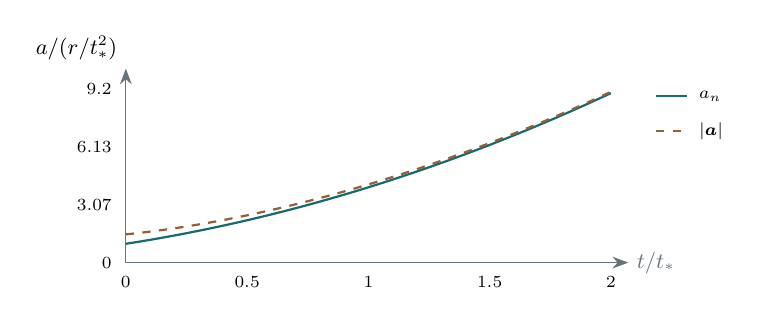
\begin{tikzpicture}[scale=.88,transform shape]
\draw[axis] (0,0.0000000)--(7.25,0.0000000) node[right] {$t/t_*$};
\draw[axis] (0.0000000,0)--(0.0000000,2.8);
\node[above left] at (0.0000000,2.8) {$a/(r/t_*^2)$};
\node[below,font=\scriptsize] at (0.0000000,-0.0800000) {$0$};
\node[below,font=\scriptsize] at (1.7500000,-0.0800000) {$0.5$};
\node[below,font=\scriptsize] at (3.5000000,-0.0800000) {$1$};
\node[below,font=\scriptsize] at (5.2500000,-0.0800000) {$1.5$};
\node[below,font=\scriptsize] at (7.0000000,-0.0800000) {$2$};
\node[left,font=\scriptsize] at (-0.0800000,0.0000000) {$0$};
\node[left,font=\scriptsize] at (-0.0800000,0.8333333) {$3.07$};
\node[left,font=\scriptsize] at (-0.0800000,1.6666667) {$6.13$};
\node[left,font=\scriptsize] at (-0.0800000,2.5000000) {$9.2$};
\draw[thick,color=accent] plot coordinates {(0.0000000,0.2717391) (0.0291667,0.2762870) (0.0583333,0.2808726) (0.0875000,0.2854959) (0.1166667,0.2901570) (0.1458333,0.2948558) (0.1750000,0.2995924) (0.2041667,0.3043667) (0.2333333,0.3091787) (0.2625000,0.3140285) (0.2916667,0.3189161) (0.3208333,0.3238413) (0.3500000,0.3288043) (0.3791667,0.3338051) (0.4083333,0.3388436) (0.4375000,0.3439198) (0.4666667,0.3490338) (0.4958333,0.3541855) (0.5250000,0.3593750) (0.5541667,0.3646022) (0.5833333,0.3698671) (0.6125000,0.3751698) (0.6416667,0.3805103) (0.6708333,0.3858884) (0.7000000,0.3913043) (0.7291667,0.3967580) (0.7583333,0.4022494) (0.7875000,0.4077785) (0.8166667,0.4133454) (0.8458333,0.4189500) (0.8750000,0.4245924) (0.9041667,0.4302725) (0.9333333,0.4359903) (0.9625000,0.4417459) (0.9916667,0.4475393) (1.0208333,0.4533703) (1.0500000,0.4592391) (1.0791667,0.4651457) (1.1083333,0.4710900) (1.1375000,0.4770720) (1.1666667,0.4830918) (1.1958333,0.4891493) (1.2250000,0.4952446) (1.2541667,0.5013776) (1.2833333,0.5075483) (1.3125000,0.5137568) (1.3416667,0.5200030) (1.3708333,0.5262870) (1.4000000,0.5326087) (1.4291667,0.5389681) (1.4583333,0.5453653) (1.4875000,0.5518003) (1.5166667,0.5582729) (1.5458333,0.5647834) (1.5750000,0.5713315) (1.6041667,0.5779174) (1.6333333,0.5845411) (1.6625000,0.5912024) (1.6916667,0.5979016) (1.7208333,0.6046384) (1.7500000,0.6114130) (1.7791667,0.6182254) (1.8083333,0.6250755) (1.8375000,0.6319633) (1.8666667,0.6388889) (1.8958333,0.6458522) (1.9250000,0.6528533) (1.9541667,0.6598921) (1.9833333,0.6669686) (2.0125000,0.6740829) (2.0416667,0.6812349) (2.0708333,0.6884247) (2.1000000,0.6956522) (2.1291667,0.7029174) (2.1583333,0.7102204) (2.1875000,0.7175611) (2.2166667,0.7249396) (2.2458333,0.7323558) (2.2750000,0.7398098) (2.3041667,0.7473015) (2.3333333,0.7548309) (2.3625000,0.7623981) (2.3916667,0.7700030) (2.4208333,0.7776457) (2.4500000,0.7853261) (2.4791667,0.7930442) (2.5083333,0.8008001) (2.5375000,0.8085938) (2.5666667,0.8164251) (2.5958333,0.8242942) (2.6250000,0.8322011) (2.6541667,0.8401457) (2.6833333,0.8481280) (2.7125000,0.8561481) (2.7416667,0.8642059) (2.7708333,0.8723015) (2.8000000,0.8804348) (2.8291667,0.8886058) (2.8583333,0.8968146) (2.8875000,0.9050611) (2.9166667,0.9133454) (2.9458333,0.9216674) (2.9750000,0.9300272) (3.0041667,0.9384247) (3.0333333,0.9468599) (3.0625000,0.9553329) (3.0916667,0.9638436) (3.1208333,0.9723921) (3.1500000,0.9809783) (3.1791667,0.9896022) (3.2083333,0.9982639) (3.2375000,1.0069633) (3.2666667,1.0157005) (3.2958333,1.0244754) (3.3250000,1.0332880) (3.3541667,1.0421384) (3.3833333,1.0510266) (3.4125000,1.0599524) (3.4416667,1.0689161) (3.4708333,1.0779174) (3.5000000,1.0869565) (3.5291667,1.0960334) (3.5583333,1.1051479) (3.5875000,1.1143003) (3.6166667,1.1234903) (3.6458333,1.1327181) (3.6750000,1.1419837) (3.7041667,1.1512870) (3.7333333,1.1606280) (3.7625000,1.1700068) (3.7916667,1.1794233) (3.8208333,1.1888776) (3.8500000,1.1983696) (3.8791667,1.2078993) (3.9083333,1.2174668) (3.9375000,1.2270720) (3.9666667,1.2367150) (3.9958333,1.2463957) (4.0250000,1.2561141) (4.0541667,1.2658703) (4.0833333,1.2756643) (4.1125000,1.2854959) (4.1416667,1.2953653) (4.1708333,1.3052725) (4.2000000,1.3152174) (4.2291667,1.3252000) (4.2583333,1.3352204) (4.2875000,1.3452785) (4.3166667,1.3553744) (4.3458333,1.3655080) (4.3750000,1.3756793) (4.4041667,1.3858884) (4.4333333,1.3961353) (4.4625000,1.4064198) (4.4916667,1.4167421) (4.5208333,1.4271022) (4.5500000,1.4375000) (4.5791667,1.4479355) (4.6083333,1.4584088) (4.6375000,1.4689198) (4.6666667,1.4794686) (4.6958333,1.4900551) (4.7250000,1.5006793) (4.7541667,1.5113413) (4.7833333,1.5220411) (4.8125000,1.5327785) (4.8416667,1.5435537) (4.8708333,1.5543667) (4.9000000,1.5652174) (4.9291667,1.5761058) (4.9583333,1.5870320) (4.9875000,1.5979959) (5.0166667,1.6089976) (5.0458333,1.6200370) (5.0750000,1.6311141) (5.1041667,1.6422290) (5.1333333,1.6533816) (5.1625000,1.6645720) (5.1916667,1.6758001) (5.2208333,1.6870660) (5.2500000,1.6983696) (5.2791667,1.7097109) (5.3083333,1.7210900) (5.3375000,1.7325068) (5.3666667,1.7439614) (5.3958333,1.7554537) (5.4250000,1.7669837) (5.4541667,1.7785515) (5.4833333,1.7901570) (5.5125000,1.8018003) (5.5416667,1.8134813) (5.5708333,1.8252000) (5.6000000,1.8369565) (5.6291667,1.8487508) (5.6583333,1.8605827) (5.6875000,1.8724524) (5.7166667,1.8843599) (5.7458333,1.8963051) (5.7750000,1.9082880) (5.8041667,1.9203087) (5.8333333,1.9323671) (5.8625000,1.9444633) (5.8916667,1.9565972) (5.9208333,1.9687689) (5.9500000,1.9809783) (5.9791667,1.9932254) (6.0083333,2.0055103) (6.0375000,2.0178329) (6.0666667,2.0301932) (6.0958333,2.0425913) (6.1250000,2.0550272) (6.1541667,2.0675008) (6.1833333,2.0800121) (6.2125000,2.0925611) (6.2416667,2.1051479) (6.2708333,2.1177725) (6.3000000,2.1304348) (6.3291667,2.1431348) (6.3583333,2.1558726) (6.3875000,2.1686481) (6.4166667,2.1814614) (6.4458333,2.1943123) (6.4750000,2.2072011) (6.5041667,2.2201276) (6.5333333,2.2330918) (6.5625000,2.2460938) (6.5916667,2.2591335) (6.6208333,2.2722109) (6.6500000,2.2853261) (6.6791667,2.2984790) (6.7083333,2.3116697) (6.7375000,2.3248981) (6.7666667,2.3381643) (6.7958333,2.3514681) (6.8250000,2.3648098) (6.8541667,2.3781892) (6.8833333,2.3916063) (6.9125000,2.4050611) (6.9416667,2.4185537) (6.9708333,2.4320841) (7.0000000,2.4456522)};
\draw[thick,color=accent] (7.65,2.4)--(8.1,2.4);\node[right,font=\scriptsize] at (8.15,2.4) {$a_n$};
\draw[thick,dashed,color=warm] plot coordinates {(0.0000000,0.4076087) (0.0291667,0.4106546) (0.0583333,0.4137537) (0.0875000,0.4169060) (0.1166667,0.4201116) (0.1458333,0.4233706) (0.1750000,0.4266829) (0.2041667,0.4300486) (0.2333333,0.4334676) (0.2625000,0.4369401) (0.2916667,0.4404658) (0.3208333,0.4440449) (0.3500000,0.4476773) (0.3791667,0.4513630) (0.4083333,0.4551018) (0.4375000,0.4588938) (0.4666667,0.4627389) (0.4958333,0.4666370) (0.5250000,0.4705880) (0.5541667,0.4745919) (0.5833333,0.4786485) (0.6125000,0.4827578) (0.6416667,0.4869197) (0.6708333,0.4911340) (0.7000000,0.4954006) (0.7291667,0.4997195) (0.7583333,0.5040905) (0.7875000,0.5085135) (0.8166667,0.5129884) (0.8458333,0.5175150) (0.8750000,0.5220933) (0.9041667,0.5267230) (0.9333333,0.5314041) (0.9625000,0.5361363) (0.9916667,0.5409197) (1.0208333,0.5457539) (1.0500000,0.5506390) (1.0791667,0.5555747) (1.1083333,0.5605608) (1.1375000,0.5655974) (1.1666667,0.5706841) (1.1958333,0.5758209) (1.2250000,0.5810076) (1.2541667,0.5862441) (1.2833333,0.5915302) (1.3125000,0.5968658) (1.3416667,0.6022506) (1.3708333,0.6076847) (1.4000000,0.6131678) (1.4291667,0.6186997) (1.4583333,0.6242804) (1.4875000,0.6299097) (1.5166667,0.6355874) (1.5458333,0.6413135) (1.5750000,0.6470876) (1.6041667,0.6529098) (1.6333333,0.6587799) (1.6625000,0.6646977) (1.6916667,0.6706631) (1.7208333,0.6766759) (1.7500000,0.6827361) (1.7791667,0.6888435) (1.8083333,0.6949979) (1.8375000,0.7011992) (1.8666667,0.7074473) (1.8958333,0.7137421) (1.9250000,0.7200834) (1.9541667,0.7264711) (1.9833333,0.7329050) (2.0125000,0.7393852) (2.0416667,0.7459113) (2.0708333,0.7524834) (2.1000000,0.7591012) (2.1291667,0.7657647) (2.1583333,0.7724738) (2.1875000,0.7792283) (2.2166667,0.7860281) (2.2458333,0.7928731) (2.2750000,0.7997632) (2.3041667,0.8066983) (2.3333333,0.8136783) (2.3625000,0.8207031) (2.3916667,0.8277725) (2.4208333,0.8348865) (2.4500000,0.8420450) (2.4791667,0.8492478) (2.5083333,0.8564949) (2.5375000,0.8637862) (2.5666667,0.8711215) (2.5958333,0.8785008) (2.6250000,0.8859240) (2.6541667,0.8933910) (2.6833333,0.9009017) (2.7125000,0.9084560) (2.7416667,0.9160538) (2.7708333,0.9236951) (2.8000000,0.9313797) (2.8291667,0.9391076) (2.8583333,0.9468786) (2.8875000,0.9546928) (2.9166667,0.9625500) (2.9458333,0.9704502) (2.9750000,0.9783932) (3.0041667,0.9863790) (3.0333333,0.9944075) (3.0625000,1.0024787) (3.0916667,1.0105925) (3.1208333,1.0187487) (3.1500000,1.0269474) (3.1791667,1.0351885) (3.2083333,1.0434718) (3.2375000,1.0517974) (3.2666667,1.0601652) (3.2958333,1.0685750) (3.3250000,1.0770269) (3.3541667,1.0855207) (3.3833333,1.0940565) (3.4125000,1.1026341) (3.4416667,1.1112535) (3.4708333,1.1199146) (3.5000000,1.1286174) (3.5291667,1.1373618) (3.5583333,1.1461478) (3.5875000,1.1549752) (3.6166667,1.1638442) (3.6458333,1.1727545) (3.6750000,1.1817062) (3.7041667,1.1906991) (3.7333333,1.1997333) (3.7625000,1.2088087) (3.7916667,1.2179253) (3.8208333,1.2270829) (3.8500000,1.2362816) (3.8791667,1.2455213) (3.9083333,1.2548020) (3.9375000,1.2641236) (3.9666667,1.2734860) (3.9958333,1.2828893) (4.0250000,1.2923333) (4.0541667,1.3018181) (4.0833333,1.3113436) (4.1125000,1.3209097) (4.1416667,1.3305165) (4.1708333,1.3401638) (4.2000000,1.3498517) (4.2291667,1.3595800) (4.2583333,1.3693488) (4.2875000,1.3791581) (4.3166667,1.3890077) (4.3458333,1.3988977) (4.3750000,1.4088280) (4.4041667,1.4187986) (4.4333333,1.4288094) (4.4625000,1.4388605) (4.4916667,1.4489517) (4.5208333,1.4590831) (4.5500000,1.4692546) (4.5791667,1.4794661) (4.6083333,1.4897177) (4.6375000,1.5000094) (4.6666667,1.5103410) (4.6958333,1.5207126) (4.7250000,1.5311242) (4.7541667,1.5415756) (4.7833333,1.5520669) (4.8125000,1.5625981) (4.8416667,1.5731690) (4.8708333,1.5837798) (4.9000000,1.5944304) (4.9291667,1.6051206) (4.9583333,1.6158506) (4.9875000,1.6266203) (5.0166667,1.6374297) (5.0458333,1.6482787) (5.0750000,1.6591673) (5.1041667,1.6700955) (5.1333333,1.6810632) (5.1625000,1.6920705) (5.1916667,1.7031174) (5.2208333,1.7142037) (5.2500000,1.7253295) (5.2791667,1.7364948) (5.3083333,1.7476995) (5.3375000,1.7589436) (5.3666667,1.7702271) (5.3958333,1.7815499) (5.4250000,1.7929122) (5.4541667,1.8043137) (5.4833333,1.8157546) (5.5125000,1.8272348) (5.5416667,1.8387542) (5.5708333,1.8503129) (5.6000000,1.8619108) (5.6291667,1.8735480) (5.6583333,1.8852243) (5.6875000,1.8969399) (5.7166667,1.9086946) (5.7458333,1.9204884) (5.7750000,1.9323214) (5.8041667,1.9441935) (5.8333333,1.9561047) (5.8625000,1.9680549) (5.8916667,1.9800443) (5.9208333,1.9920727) (5.9500000,2.0041401) (5.9791667,2.0162466) (6.0083333,2.0283920) (6.0375000,2.0405764) (6.0666667,2.0527999) (6.0958333,2.0650622) (6.1250000,2.0773636) (6.1541667,2.0897038) (6.1833333,2.1020830) (6.2125000,2.1145011) (6.2416667,2.1269581) (6.2708333,2.1394539) (6.3000000,2.1519886) (6.3291667,2.1645622) (6.3583333,2.1771746) (6.3875000,2.1898259) (6.4166667,2.2025159) (6.4458333,2.2152448) (6.4750000,2.2280124) (6.5041667,2.2408188) (6.5333333,2.2536640) (6.5625000,2.2665480) (6.5916667,2.2794707) (6.6208333,2.2924321) (6.6500000,2.3054323) (6.6791667,2.3184712) (6.7083333,2.3315487) (6.7375000,2.3446650) (6.7666667,2.3578199) (6.7958333,2.3710135) (6.8250000,2.3842458) (6.8541667,2.3975167) (6.8833333,2.4108263) (6.9125000,2.4241745) (6.9416667,2.4375613) (6.9708333,2.4509867) (7.0000000,2.4644507)};
\draw[thick,dashed,color=warm] (7.65,1.9)--(8.1,1.9);\node[right,font=\scriptsize] at (8.15,1.9) {$|\boldsymbol a|$};
\end{tikzpicture}
\figcaption{变图综二.1V5\quad 非匀速螺线的法向和总加速度}
\end{minipage}\end{center}
\item \textbf{由曲率反求螺距。}已知圆柱半径$r$和螺线曲率半径$\rho$，求螺距大小。

由$\rho=r+h^2/(4\pi^2r)$移项，
\[|h|=2\pi\sqrt{r(\rho-r)},\qquad \rho\ge r.\]
图V6画非负螺距分支；$\rho=r$时为水平圆，$\rho=2r$时$|h|=2\pi r$。曲率给出螺距的大小；旋向由$h$的正负另行说明，左右旋螺线具有同一曲率半径。
\begin{center}\begin{minipage}{.98\linewidth}\centering
\begin{tikzpicture}[scale=.88,transform shape]
\draw[axis] (0,0.0000000)--(7.25,0.0000000) node[right] {$\rho/r$};
\draw[axis] (0.0000000,0)--(0.0000000,2.8);
\node[above left] at (0.0000000,2.8) {$h/(2\pi r)$};
\node[below,font=\scriptsize] at (0.0000000,-0.0800000) {$1$};
\node[below,font=\scriptsize] at (1.7500000,-0.0800000) {$2$};
\node[below,font=\scriptsize] at (3.5000000,-0.0800000) {$3$};
\node[below,font=\scriptsize] at (5.2500000,-0.0800000) {$4$};
\node[below,font=\scriptsize] at (7.0000000,-0.0800000) {$5$};
\node[left,font=\scriptsize] at (-0.0800000,0.0000000) {$0$};
\node[left,font=\scriptsize] at (-0.0800000,0.8333333) {$0.733$};
\node[left,font=\scriptsize] at (-0.0800000,1.6666667) {$1.47$};
\node[left,font=\scriptsize] at (-0.0800000,2.5000000) {$2.2$};
\draw[thick,color=accent] plot coordinates {(0.0000000,0.0000000) (0.0291667,0.1467039) (0.0583333,0.2074707) (0.0875000,0.2540986) (0.1166667,0.2934078) (0.1458333,0.3280399) (0.1750000,0.3593497) (0.2041667,0.3881421) (0.2333333,0.4149413) (0.2625000,0.4401117) (0.2916667,0.4639185) (0.3208333,0.4865618) (0.3500000,0.5081973) (0.3791667,0.5289485) (0.4083333,0.5489158) (0.4375000,0.5681818) (0.4666667,0.5868157) (0.4958333,0.6048757) (0.5250000,0.6224120) (0.5541667,0.6394675) (0.5833333,0.6560799) (0.6125000,0.6722818) (0.6416667,0.6881024) (0.6708333,0.7035673) (0.7000000,0.7186995) (0.7291667,0.7335196) (0.7583333,0.7480461) (0.7875000,0.7622959) (0.8166667,0.7762841) (0.8458333,0.7900248) (0.8750000,0.8035304) (0.9041667,0.8168128) (0.9333333,0.8298827) (0.9625000,0.8427498) (0.9916667,0.8554235) (1.0208333,0.8679121) (1.0500000,0.8802235) (1.0791667,0.8923651) (1.1083333,0.9043437) (1.1375000,0.9161657) (1.1666667,0.9278370) (1.1958333,0.9393634) (1.2250000,0.9507500) (1.2541667,0.9620019) (1.2833333,0.9731237) (1.3125000,0.9841198) (1.3416667,0.9949944) (1.3708333,1.0057514) (1.4000000,1.0163945) (1.4291667,1.0269274) (1.4583333,1.0373533) (1.4875000,1.0476755) (1.5166667,1.0578970) (1.5458333,1.0680206) (1.5750000,1.0780492) (1.6041667,1.0879853) (1.6333333,1.0978316) (1.6625000,1.1075903) (1.6916667,1.1172637) (1.7208333,1.1268542) (1.7500000,1.1363636) (1.7791667,1.1457942) (1.8083333,1.1551478) (1.8375000,1.1644262) (1.8666667,1.1736313) (1.8958333,1.1827648) (1.9250000,1.1918282) (1.9541667,1.2008233) (1.9833333,1.2097515) (2.0125000,1.2186142) (2.0416667,1.2274130) (2.0708333,1.2361492) (2.1000000,1.2448240) (2.1291667,1.2534388) (2.1583333,1.2619948) (2.1875000,1.2704932) (2.2166667,1.2789351) (2.2458333,1.2873216) (2.2750000,1.2956539) (2.3041667,1.3039329) (2.3333333,1.3121597) (2.3625000,1.3203352) (2.3916667,1.3284604) (2.4208333,1.3365363) (2.4500000,1.3445636) (2.4791667,1.3525433) (2.5083333,1.3604761) (2.5375000,1.3683630) (2.5666667,1.3762047) (2.5958333,1.3840020) (2.6250000,1.3917555) (2.6541667,1.3994662) (2.6833333,1.4071345) (2.7125000,1.4147613) (2.7416667,1.4223472) (2.7708333,1.4298929) (2.8000000,1.4373989) (2.8291667,1.4448660) (2.8583333,1.4522947) (2.8875000,1.4596855) (2.9166667,1.4670391) (2.9458333,1.4743561) (2.9750000,1.4816369) (3.0041667,1.4888821) (3.0333333,1.4960922) (3.0625000,1.5032678) (3.0916667,1.5104092) (3.1208333,1.5175171) (3.1500000,1.5245918) (3.1791667,1.5316338) (3.2083333,1.5386436) (3.2375000,1.5456216) (3.2666667,1.5525683) (3.2958333,1.5594840) (3.3250000,1.5663692) (3.3541667,1.5732242) (3.3833333,1.5800495) (3.4125000,1.5868455) (3.4416667,1.5936124) (3.4708333,1.6003508) (3.5000000,1.6070609) (3.5291667,1.6137431) (3.5583333,1.6203977) (3.5875000,1.6270251) (3.6166667,1.6336257) (3.6458333,1.6401996) (3.6750000,1.6467474) (3.7041667,1.6532692) (3.7333333,1.6597653) (3.7625000,1.6662362) (3.7916667,1.6726820) (3.8208333,1.6791030) (3.8500000,1.6854997) (3.8791667,1.6918721) (3.9083333,1.6982206) (3.9375000,1.7045455) (3.9666667,1.7108469) (3.9958333,1.7171253) (4.0250000,1.7233808) (4.0541667,1.7296136) (4.0833333,1.7358241) (4.1125000,1.7420125) (4.1416667,1.7481789) (4.1708333,1.7543237) (4.2000000,1.7604470) (4.2291667,1.7665491) (4.2583333,1.7726301) (4.2875000,1.7786904) (4.3166667,1.7847301) (4.3458333,1.7907495) (4.3750000,1.7967487) (4.4041667,1.8027279) (4.4333333,1.8086873) (4.4625000,1.8146272) (4.4916667,1.8205477) (4.5208333,1.8264490) (4.5500000,1.8323313) (4.5791667,1.8381948) (4.6083333,1.8440396) (4.6375000,1.8498660) (4.6666667,1.8556740) (4.6958333,1.8614640) (4.7250000,1.8672360) (4.7541667,1.8729902) (4.7833333,1.8787268) (4.8125000,1.8844459) (4.8416667,1.8901477) (4.8708333,1.8958324) (4.9000000,1.9015001) (4.9291667,1.9071509) (4.9583333,1.9127850) (4.9875000,1.9184026) (5.0166667,1.9240038) (5.0458333,1.9295887) (5.0750000,1.9351575) (5.1041667,1.9407104) (5.1333333,1.9462474) (5.1625000,1.9517686) (5.1916667,1.9572743) (5.2208333,1.9627646) (5.2500000,1.9682396) (5.2791667,1.9736993) (5.3083333,1.9791440) (5.3375000,1.9845738) (5.3666667,1.9899887) (5.3958333,1.9953890) (5.4250000,2.0007746) (5.4541667,2.0061459) (5.4833333,2.0115027) (5.5125000,2.0168454) (5.5416667,2.0221739) (5.5708333,2.0274884) (5.6000000,2.0327891) (5.6291667,2.0380759) (5.6583333,2.0433491) (5.6875000,2.0486087) (5.7166667,2.0538548) (5.7458333,2.0590876) (5.7750000,2.0643071) (5.8041667,2.0695134) (5.8333333,2.0747067) (5.8625000,2.0798870) (5.8916667,2.0850544) (5.9208333,2.0902090) (5.9500000,2.0953510) (5.9791667,2.1004804) (6.0083333,2.1055973) (6.0375000,2.1107018) (6.0666667,2.1157939) (6.0958333,2.1208739) (6.1250000,2.1259417) (6.1541667,2.1309975) (6.1833333,2.1360412) (6.2125000,2.1410731) (6.2416667,2.1460933) (6.2708333,2.1511016) (6.3000000,2.1560984) (6.3291667,2.1610836) (6.3583333,2.1660573) (6.3875000,2.1710197) (6.4166667,2.1759707) (6.4458333,2.1809105) (6.4750000,2.1858391) (6.5041667,2.1907566) (6.5333333,2.1956631) (6.5625000,2.2005587) (6.5916667,2.2054434) (6.6208333,2.2103173) (6.6500000,2.2151805) (6.6791667,2.2200331) (6.7083333,2.2248750) (6.7375000,2.2297065) (6.7666667,2.2345275) (6.7958333,2.2393381) (6.8250000,2.2441384) (6.8541667,2.2489284) (6.8833333,2.2537083) (6.9125000,2.2584781) (6.9416667,2.2632378) (6.9708333,2.2679875) (7.0000000,2.2727273)};
\end{tikzpicture}
\figcaption{变图综二.1V6\quad 曲率半径反求非负螺距}
\end{minipage}\end{center}
\item \textbf{两个主曲率均非零。}局部曲面用切平面坐标写成$w=(\kappa_a s_1^2+\kappa_b s_2^2)/2+O(s^3)$。求与$s_1$成角$\varphi$的正截面曲率，并求其正交方向的曲率和。

在正截面中代入$s_1=s\cos\varphi,s_2=s\sin\varphi$，二阶项为
\[w=\tfrac12(\kappa_a\cos^2\varphi+\kappa_b\sin^2\varphi)s^2+O(s^3).\]
故$\kappa(\varphi)=\kappa_a\cos^2\varphi+\kappa_b\sin^2\varphi$，加上正交方向即为$\kappa_a+\kappa_b$。图V7取$\kappa_a=1/r,\kappa_b=1/(2r)$，两曲线之和为$3/2$；圆柱对应$\kappa_b=0$，球面对应两主曲率相等。
\begin{center}\begin{minipage}{.98\linewidth}\centering
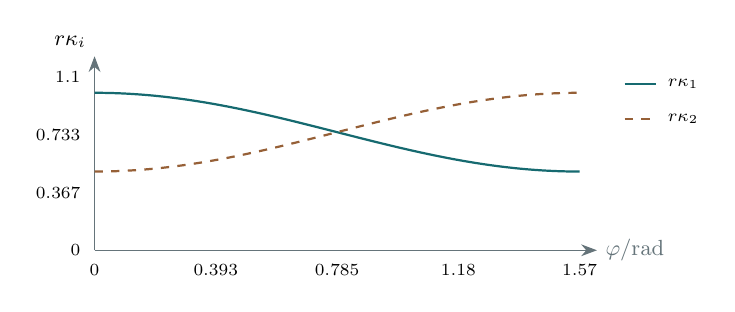
\begin{tikzpicture}[scale=.88,transform shape]
\draw[axis] (0,0.0000000)--(7.25,0.0000000) node[right] {$\varphi/\mathrm{rad}$};
\draw[axis] (0.0000000,0)--(0.0000000,2.8);
\node[above left] at (0.0000000,2.8) {$r\kappa_i$};
\node[below,font=\scriptsize] at (0.0000000,-0.0800000) {$0$};
\node[below,font=\scriptsize] at (1.7500000,-0.0800000) {$0.393$};
\node[below,font=\scriptsize] at (3.5000000,-0.0800000) {$0.785$};
\node[below,font=\scriptsize] at (5.2500000,-0.0800000) {$1.18$};
\node[below,font=\scriptsize] at (7.0000000,-0.0800000) {$1.57$};
\node[left,font=\scriptsize] at (-0.0800000,0.0000000) {$0$};
\node[left,font=\scriptsize] at (-0.0800000,0.8333333) {$0.367$};
\node[left,font=\scriptsize] at (-0.0800000,1.6666667) {$0.733$};
\node[left,font=\scriptsize] at (-0.0800000,2.5000000) {$1.1$};
\draw[thick,color=accent] plot coordinates {(0.0000000,2.2727273) (0.0291667,2.2726786) (0.0583333,2.2725326) (0.0875000,2.2722892) (0.1166667,2.2719486) (0.1458333,2.2715108) (0.1750000,2.2709758) (0.2041667,2.2703437) (0.2333333,2.2696147) (0.2625000,2.2687889) (0.2916667,2.2678664) (0.3208333,2.2668474) (0.3500000,2.2657320) (0.3791667,2.2645205) (0.4083333,2.2632130) (0.4375000,2.2618098) (0.4666667,2.2603111) (0.4958333,2.2587172) (0.5250000,2.2570284) (0.5541667,2.2552448) (0.5833333,2.2533669) (0.6125000,2.2513950) (0.6416667,2.2493294) (0.6708333,2.2471704) (0.7000000,2.2449185) (0.7291667,2.2425739) (0.7583333,2.2401372) (0.7875000,2.2376087) (0.8166667,2.2349889) (0.8458333,2.2322782) (0.8750000,2.2294770) (0.9041667,2.2265859) (0.9333333,2.2236054) (0.9625000,2.2205359) (0.9916667,2.2173780) (1.0208333,2.2141322) (1.0500000,2.2107992) (1.0791667,2.2073793) (1.1083333,2.2038734) (1.1375000,2.2002818) (1.1666667,2.1966053) (1.1958333,2.1928446) (1.2250000,2.1890001) (1.2541667,2.1850726) (1.2833333,2.1810628) (1.3125000,2.1769714) (1.3416667,2.1727990) (1.3708333,2.1685463) (1.4000000,2.1642142) (1.4291667,2.1598033) (1.4583333,2.1553144) (1.4875000,2.1507483) (1.5166667,2.1461057) (1.5458333,2.1413874) (1.5750000,2.1365943) (1.6041667,2.1317272) (1.6333333,2.1267868) (1.6625000,2.1217742) (1.6916667,2.1166900) (1.7208333,2.1115352) (1.7500000,2.1063107) (1.7791667,2.1010173) (1.8083333,2.0956560) (1.8375000,2.0902277) (1.8666667,2.0847333) (1.8958333,2.0791738) (1.9250000,2.0735500) (1.9541667,2.0678631) (1.9833333,2.0621139) (2.0125000,2.0563034) (2.0416667,2.0504326) (2.0708333,2.0445026) (2.1000000,2.0385143) (2.1291667,2.0324689) (2.1583333,2.0263672) (2.1875000,2.0202104) (2.2166667,2.0139995) (2.2458333,2.0077355) (2.2750000,2.0014196) (2.3041667,1.9950529) (2.3333333,1.9886364) (2.3625000,1.9821712) (2.3916667,1.9756584) (2.4208333,1.9690992) (2.4500000,1.9624946) (2.4791667,1.9558458) (2.5083333,1.9491540) (2.5375000,1.9424203) (2.5666667,1.9356458) (2.5958333,1.9288317) (2.6250000,1.9219792) (2.6541667,1.9150895) (2.6833333,1.9081636) (2.7125000,1.9012029) (2.7416667,1.8942084) (2.7708333,1.8871815) (2.8000000,1.8801233) (2.8291667,1.8730350) (2.8583333,1.8659178) (2.8875000,1.8587730) (2.9166667,1.8516017) (2.9458333,1.8444053) (2.9750000,1.8371849) (3.0041667,1.8299417) (3.0333333,1.8226771) (3.0625000,1.8153922) (3.0916667,1.8080884) (3.1208333,1.8007668) (3.1500000,1.7934287) (3.1791667,1.7860754) (3.2083333,1.7787081) (3.2375000,1.7713281) (3.2666667,1.7639366) (3.2958333,1.7565350) (3.3250000,1.7491245) (3.3541667,1.7417063) (3.3833333,1.7342818) (3.4125000,1.7268522) (3.4416667,1.7194187) (3.4708333,1.7119827) (3.5000000,1.7045455) (3.5291667,1.6971082) (3.5583333,1.6896722) (3.5875000,1.6822387) (3.6166667,1.6748091) (3.6458333,1.6673846) (3.6750000,1.6599664) (3.7041667,1.6525559) (3.7333333,1.6451543) (3.7625000,1.6377628) (3.7916667,1.6303828) (3.8208333,1.6230156) (3.8500000,1.6156622) (3.8791667,1.6083241) (3.9083333,1.6010025) (3.9375000,1.5936987) (3.9666667,1.5864138) (3.9958333,1.5791492) (4.0250000,1.5719060) (4.0541667,1.5646856) (4.0833333,1.5574892) (4.1125000,1.5503179) (4.1416667,1.5431731) (4.1708333,1.5360559) (4.2000000,1.5289676) (4.2291667,1.5219094) (4.2583333,1.5148825) (4.2875000,1.5078880) (4.3166667,1.5009273) (4.3458333,1.4940015) (4.3750000,1.4871117) (4.4041667,1.4802592) (4.4333333,1.4734451) (4.4625000,1.4666706) (4.4916667,1.4599369) (4.5208333,1.4532451) (4.5500000,1.4465963) (4.5791667,1.4399917) (4.6083333,1.4334325) (4.6375000,1.4269197) (4.6666667,1.4204545) (4.6958333,1.4140380) (4.7250000,1.4076713) (4.7541667,1.4013554) (4.7833333,1.3950915) (4.8125000,1.3888805) (4.8416667,1.3827237) (4.8708333,1.3766221) (4.9000000,1.3705766) (4.9291667,1.3645883) (4.9583333,1.3586583) (4.9875000,1.3527875) (5.0166667,1.3469771) (5.0458333,1.3412278) (5.0750000,1.3355409) (5.1041667,1.3299172) (5.1333333,1.3243576) (5.1625000,1.3188632) (5.1916667,1.3134349) (5.2208333,1.3080736) (5.2500000,1.3027802) (5.2791667,1.2975557) (5.3083333,1.2924009) (5.3375000,1.2873168) (5.3666667,1.2823041) (5.3958333,1.2773637) (5.4250000,1.2724966) (5.4541667,1.2677035) (5.4833333,1.2629852) (5.5125000,1.2583427) (5.5416667,1.2537765) (5.5708333,1.2492876) (5.6000000,1.2448767) (5.6291667,1.2405446) (5.6583333,1.2362919) (5.6875000,1.2321195) (5.7166667,1.2280281) (5.7458333,1.2240183) (5.7750000,1.2200908) (5.8041667,1.2162464) (5.8333333,1.2124856) (5.8625000,1.2088091) (5.8916667,1.2052175) (5.9208333,1.2017116) (5.9500000,1.1982917) (5.9791667,1.1949587) (6.0083333,1.1917129) (6.0375000,1.1885550) (6.0666667,1.1854855) (6.0958333,1.1825050) (6.1250000,1.1796139) (6.1541667,1.1768128) (6.1833333,1.1741020) (6.2125000,1.1714822) (6.2416667,1.1689537) (6.2708333,1.1665170) (6.3000000,1.1641724) (6.3291667,1.1619205) (6.3583333,1.1597615) (6.3875000,1.1576959) (6.4166667,1.1557240) (6.4458333,1.1538461) (6.4750000,1.1520625) (6.5041667,1.1503737) (6.5333333,1.1487798) (6.5625000,1.1472811) (6.5916667,1.1458779) (6.6208333,1.1445704) (6.6500000,1.1433589) (6.6791667,1.1422435) (6.7083333,1.1412245) (6.7375000,1.1403020) (6.7666667,1.1394762) (6.7958333,1.1387472) (6.8250000,1.1381152) (6.8541667,1.1375802) (6.8833333,1.1371423) (6.9125000,1.1368017) (6.9416667,1.1365583) (6.9708333,1.1364123) (7.0000000,1.1363636)};
\draw[thick,color=accent] (7.65,2.4)--(8.1,2.4);\node[right,font=\scriptsize] at (8.15,2.4) {$r\kappa_1$};
\draw[thick,dashed,color=warm] plot coordinates {(0.0000000,1.1363636) (0.0291667,1.1364123) (0.0583333,1.1365583) (0.0875000,1.1368017) (0.1166667,1.1371423) (0.1458333,1.1375802) (0.1750000,1.1381152) (0.2041667,1.1387472) (0.2333333,1.1394762) (0.2625000,1.1403020) (0.2916667,1.1412245) (0.3208333,1.1422435) (0.3500000,1.1433589) (0.3791667,1.1445704) (0.4083333,1.1458779) (0.4375000,1.1472811) (0.4666667,1.1487798) (0.4958333,1.1503737) (0.5250000,1.1520625) (0.5541667,1.1538461) (0.5833333,1.1557240) (0.6125000,1.1576959) (0.6416667,1.1597615) (0.6708333,1.1619205) (0.7000000,1.1641724) (0.7291667,1.1665170) (0.7583333,1.1689537) (0.7875000,1.1714822) (0.8166667,1.1741020) (0.8458333,1.1768128) (0.8750000,1.1796139) (0.9041667,1.1825050) (0.9333333,1.1854855) (0.9625000,1.1885550) (0.9916667,1.1917129) (1.0208333,1.1949587) (1.0500000,1.1982917) (1.0791667,1.2017116) (1.1083333,1.2052175) (1.1375000,1.2088091) (1.1666667,1.2124856) (1.1958333,1.2162464) (1.2250000,1.2200908) (1.2541667,1.2240183) (1.2833333,1.2280281) (1.3125000,1.2321195) (1.3416667,1.2362919) (1.3708333,1.2405446) (1.4000000,1.2448767) (1.4291667,1.2492876) (1.4583333,1.2537765) (1.4875000,1.2583427) (1.5166667,1.2629852) (1.5458333,1.2677035) (1.5750000,1.2724966) (1.6041667,1.2773637) (1.6333333,1.2823041) (1.6625000,1.2873168) (1.6916667,1.2924009) (1.7208333,1.2975557) (1.7500000,1.3027802) (1.7791667,1.3080736) (1.8083333,1.3134349) (1.8375000,1.3188632) (1.8666667,1.3243576) (1.8958333,1.3299172) (1.9250000,1.3355409) (1.9541667,1.3412278) (1.9833333,1.3469771) (2.0125000,1.3527875) (2.0416667,1.3586583) (2.0708333,1.3645883) (2.1000000,1.3705766) (2.1291667,1.3766221) (2.1583333,1.3827237) (2.1875000,1.3888805) (2.2166667,1.3950915) (2.2458333,1.4013554) (2.2750000,1.4076713) (2.3041667,1.4140380) (2.3333333,1.4204545) (2.3625000,1.4269197) (2.3916667,1.4334325) (2.4208333,1.4399917) (2.4500000,1.4465963) (2.4791667,1.4532451) (2.5083333,1.4599369) (2.5375000,1.4666706) (2.5666667,1.4734451) (2.5958333,1.4802592) (2.6250000,1.4871117) (2.6541667,1.4940015) (2.6833333,1.5009273) (2.7125000,1.5078880) (2.7416667,1.5148825) (2.7708333,1.5219094) (2.8000000,1.5289676) (2.8291667,1.5360559) (2.8583333,1.5431731) (2.8875000,1.5503179) (2.9166667,1.5574892) (2.9458333,1.5646856) (2.9750000,1.5719060) (3.0041667,1.5791492) (3.0333333,1.5864138) (3.0625000,1.5936987) (3.0916667,1.6010025) (3.1208333,1.6083241) (3.1500000,1.6156622) (3.1791667,1.6230156) (3.2083333,1.6303828) (3.2375000,1.6377628) (3.2666667,1.6451543) (3.2958333,1.6525559) (3.3250000,1.6599664) (3.3541667,1.6673846) (3.3833333,1.6748091) (3.4125000,1.6822387) (3.4416667,1.6896722) (3.4708333,1.6971082) (3.5000000,1.7045455) (3.5291667,1.7119827) (3.5583333,1.7194187) (3.5875000,1.7268522) (3.6166667,1.7342818) (3.6458333,1.7417063) (3.6750000,1.7491245) (3.7041667,1.7565350) (3.7333333,1.7639366) (3.7625000,1.7713281) (3.7916667,1.7787081) (3.8208333,1.7860754) (3.8500000,1.7934287) (3.8791667,1.8007668) (3.9083333,1.8080884) (3.9375000,1.8153922) (3.9666667,1.8226771) (3.9958333,1.8299417) (4.0250000,1.8371849) (4.0541667,1.8444053) (4.0833333,1.8516017) (4.1125000,1.8587730) (4.1416667,1.8659178) (4.1708333,1.8730350) (4.2000000,1.8801233) (4.2291667,1.8871815) (4.2583333,1.8942084) (4.2875000,1.9012029) (4.3166667,1.9081636) (4.3458333,1.9150895) (4.3750000,1.9219792) (4.4041667,1.9288317) (4.4333333,1.9356458) (4.4625000,1.9424203) (4.4916667,1.9491540) (4.5208333,1.9558458) (4.5500000,1.9624946) (4.5791667,1.9690992) (4.6083333,1.9756584) (4.6375000,1.9821712) (4.6666667,1.9886364) (4.6958333,1.9950529) (4.7250000,2.0014196) (4.7541667,2.0077355) (4.7833333,2.0139995) (4.8125000,2.0202104) (4.8416667,2.0263672) (4.8708333,2.0324689) (4.9000000,2.0385143) (4.9291667,2.0445026) (4.9583333,2.0504326) (4.9875000,2.0563034) (5.0166667,2.0621139) (5.0458333,2.0678631) (5.0750000,2.0735500) (5.1041667,2.0791738) (5.1333333,2.0847333) (5.1625000,2.0902277) (5.1916667,2.0956560) (5.2208333,2.1010173) (5.2500000,2.1063107) (5.2791667,2.1115352) (5.3083333,2.1166900) (5.3375000,2.1217742) (5.3666667,2.1267868) (5.3958333,2.1317272) (5.4250000,2.1365943) (5.4541667,2.1413874) (5.4833333,2.1461057) (5.5125000,2.1507483) (5.5416667,2.1553144) (5.5708333,2.1598033) (5.6000000,2.1642142) (5.6291667,2.1685463) (5.6583333,2.1727990) (5.6875000,2.1769714) (5.7166667,2.1810628) (5.7458333,2.1850726) (5.7750000,2.1890001) (5.8041667,2.1928446) (5.8333333,2.1966053) (5.8625000,2.2002818) (5.8916667,2.2038734) (5.9208333,2.2073793) (5.9500000,2.2107992) (5.9791667,2.2141322) (6.0083333,2.2173780) (6.0375000,2.2205359) (6.0666667,2.2236054) (6.0958333,2.2265859) (6.1250000,2.2294770) (6.1541667,2.2322782) (6.1833333,2.2349889) (6.2125000,2.2376087) (6.2416667,2.2401372) (6.2708333,2.2425739) (6.3000000,2.2449185) (6.3291667,2.2471704) (6.3583333,2.2493294) (6.3875000,2.2513950) (6.4166667,2.2533669) (6.4458333,2.2552448) (6.4750000,2.2570284) (6.5041667,2.2587172) (6.5333333,2.2603111) (6.5625000,2.2618098) (6.5916667,2.2632130) (6.6208333,2.2645205) (6.6500000,2.2657320) (6.6791667,2.2668474) (6.7083333,2.2678664) (6.7375000,2.2687889) (6.7666667,2.2696147) (6.7958333,2.2703437) (6.8250000,2.2709758) (6.8541667,2.2715108) (6.8833333,2.2719486) (6.9125000,2.2722892) (6.9416667,2.2725326) (6.9708333,2.2726786) (7.0000000,2.2727273)};
\draw[thick,dashed,color=warm] (7.65,1.9)--(8.1,1.9);\node[right,font=\scriptsize] at (8.15,1.9) {$r\kappa_2$};
\end{tikzpicture}
\figcaption{变图综二.1V7\quad 两主曲率不等时正交曲率的互补变化}
\end{minipage}\end{center}
\item \textbf{固定速率的螺线导轨。}质量$m$的质点以固定速率$v$沿半径$r$、螺距$h$的螺线运动，求沿曲率法线的合力大小。

令$a=h/(2\pi)$，由$\rho=(r^2+a^2)/r$，
\[F_n=mv^2/\rho=\frac{mv^2r}{r^2+a^2},\qquad F_n/(mv^2/r)=\frac1{1+[h/(2\pi r)]^2}.\]
图V8显示螺距增大时法向力减小。此时总速率固定，圆周分速度为$vr/\sqrt{r^2+a^2}$，其平方除以$r$给同一个法向加速度。轴向分速度占比增大，使轨迹在局部更平直。
\begin{center}\begin{minipage}{.98\linewidth}\centering
\begin{tikzpicture}[scale=.88,transform shape]
\draw[axis] (0,0.0000000)--(7.25,0.0000000) node[right] {$h/(2\pi r)$};
\draw[axis] (0.0000000,0)--(0.0000000,2.8);
\node[above left] at (0.0000000,2.8) {$F_n/(mv^2/r)$};
\node[below,font=\scriptsize] at (0.0000000,-0.0800000) {$0$};
\node[below,font=\scriptsize] at (1.7500000,-0.0800000) {$0.5$};
\node[below,font=\scriptsize] at (3.5000000,-0.0800000) {$1$};
\node[below,font=\scriptsize] at (5.2500000,-0.0800000) {$1.5$};
\node[below,font=\scriptsize] at (7.0000000,-0.0800000) {$2$};
\node[left,font=\scriptsize] at (-0.0800000,0.0000000) {$0$};
\node[left,font=\scriptsize] at (-0.0800000,0.8333333) {$0.367$};
\node[left,font=\scriptsize] at (-0.0800000,1.6666667) {$0.733$};
\node[left,font=\scriptsize] at (-0.0800000,2.5000000) {$1.1$};
\draw[thick,color=accent] plot coordinates {(0.0000000,2.2727273) (0.0291667,2.2725695) (0.0583333,2.2720961) (0.0875000,2.2713077) (0.1166667,2.2702048) (0.1458333,2.2687884) (0.1750000,2.2670596) (0.2041667,2.2650199) (0.2333333,2.2626710) (0.2625000,2.2600147) (0.2916667,2.2570533) (0.3208333,2.2537892) (0.3500000,2.2502250) (0.3791667,2.2463637) (0.4083333,2.2422083) (0.4375000,2.2377622) (0.4666667,2.2330290) (0.4958333,2.2280123) (0.5250000,2.2227162) (0.5541667,2.2171447) (0.5833333,2.2113022) (0.6125000,2.2051932) (0.6416667,2.1988224) (0.6708333,2.1921946) (0.7000000,2.1853147) (0.7291667,2.1781879) (0.7583333,2.1708194) (0.7875000,2.1632145) (0.8166667,2.1553789) (0.8458333,2.1473179) (0.8750000,2.1390374) (0.9041667,2.1305431) (0.9333333,2.1218408) (0.9625000,2.1129365) (0.9916667,2.1038360) (1.0208333,2.0945455) (1.0500000,2.0850709) (1.0791667,2.0754184) (1.1083333,2.0655941) (1.1375000,2.0556041) (1.1666667,2.0454545) (1.1958333,2.0351516) (1.2250000,2.0247014) (1.2541667,2.0141100) (1.2833333,2.0033835) (1.3125000,1.9925280) (1.3416667,1.9815496) (1.3708333,1.9704541) (1.4000000,1.9592476) (1.4291667,1.9479360) (1.4583333,1.9365250) (1.4875000,1.9250205) (1.5166667,1.9134280) (1.5458333,1.9017533) (1.5750000,1.8900019) (1.6041667,1.8781792) (1.6333333,1.8662906) (1.6625000,1.8543415) (1.6916667,1.8423369) (1.7208333,1.8302820) (1.7500000,1.8181818) (1.7791667,1.8060412) (1.8083333,1.7938650) (1.8375000,1.7816578) (1.8666667,1.7694243) (1.8958333,1.7571690) (1.9250000,1.7448962) (1.9541667,1.7326101) (1.9833333,1.7203150) (2.0125000,1.7080149) (2.0416667,1.6957136) (2.0708333,1.6834151) (2.1000000,1.6711230) (2.1291667,1.6588409) (2.1583333,1.6465724) (2.1875000,1.6343207) (2.2166667,1.6220893) (2.2458333,1.6098811) (2.2750000,1.5976993) (2.3041667,1.5855469) (2.3333333,1.5734266) (2.3625000,1.5613412) (2.3916667,1.5492934) (2.4208333,1.5372856) (2.4500000,1.5253203) (2.4791667,1.5133999) (2.5083333,1.5015266) (2.5375000,1.4897024) (2.5666667,1.4779296) (2.5958333,1.4662100) (2.6250000,1.4545455) (2.6541667,1.4429378) (2.6833333,1.4313888) (2.7125000,1.4198999) (2.7416667,1.4084727) (2.7708333,1.3971088) (2.8000000,1.3858093) (2.8291667,1.3745757) (2.8583333,1.3634091) (2.8875000,1.3523108) (2.9166667,1.3412817) (2.9458333,1.3303229) (2.9750000,1.3194353) (3.0041667,1.3086198) (3.0333333,1.2978772) (3.0625000,1.2872084) (3.0916667,1.2766139) (3.1208333,1.2660943) (3.1500000,1.2556504) (3.1791667,1.2452826) (3.2083333,1.2349914) (3.2375000,1.2247772) (3.2666667,1.2146405) (3.2958333,1.2045814) (3.3250000,1.1946004) (3.3541667,1.1846977) (3.3833333,1.1748734) (3.4125000,1.1651277) (3.4416667,1.1554608) (3.4708333,1.1458728) (3.5000000,1.1363636) (3.5291667,1.1269334) (3.5583333,1.1175820) (3.5875000,1.1083096) (3.6166667,1.0991158) (3.6458333,1.0900008) (3.6750000,1.0809642) (3.7041667,1.0720061) (3.7333333,1.0631261) (3.7625000,1.0543240) (3.7916667,1.0455998) (3.8208333,1.0369530) (3.8500000,1.0283834) (3.8791667,1.0198907) (3.9083333,1.0114746) (3.9375000,1.0031348) (3.9666667,0.9948709) (3.9958333,0.9866825) (4.0250000,0.9785693) (4.0541667,0.9705309) (4.0833333,0.9625668) (4.1125000,0.9546767) (4.1416667,0.9468601) (4.1708333,0.9391166) (4.2000000,0.9314456) (4.2291667,0.9238468) (4.2583333,0.9163197) (4.2875000,0.9088637) (4.3166667,0.9014784) (4.3458333,0.8941633) (4.3750000,0.8869180) (4.4041667,0.8797417) (4.4333333,0.8726342) (4.4625000,0.8655948) (4.4916667,0.8586230) (4.5208333,0.8517182) (4.5500000,0.8448800) (4.5791667,0.8381078) (4.6083333,0.8314011) (4.6375000,0.8247593) (4.6666667,0.8181818) (4.6958333,0.8116682) (4.7250000,0.8052178) (4.7541667,0.7988302) (4.7833333,0.7925047) (4.8125000,0.7862408) (4.8416667,0.7800380) (4.8708333,0.7738956) (4.9000000,0.7678133) (4.9291667,0.7617903) (4.9583333,0.7558262) (4.9875000,0.7499203) (5.0166667,0.7440722) (5.0458333,0.7382813) (5.0750000,0.7325471) (5.1041667,0.7268689) (5.1333333,0.7212463) (5.1625000,0.7156787) (5.1916667,0.7101656) (5.2208333,0.7047065) (5.2500000,0.6993007) (5.2791667,0.6939478) (5.3083333,0.6886473) (5.3375000,0.6833985) (5.3666667,0.6782011) (5.3958333,0.6730545) (5.4250000,0.6679581) (5.4541667,0.6629114) (5.4833333,0.6579140) (5.5125000,0.6529653) (5.5416667,0.6480648) (5.5708333,0.6432121) (5.6000000,0.6384065) (5.6291667,0.6336478) (5.6583333,0.6289352) (5.6875000,0.6242684) (5.7166667,0.6196469) (5.7458333,0.6150702) (5.7750000,0.6105379) (5.8041667,0.6060494) (5.8333333,0.6016043) (5.8625000,0.5972021) (5.8916667,0.5928424) (5.9208333,0.5885247) (5.9500000,0.5842487) (5.9791667,0.5800137) (6.0083333,0.5758194) (6.0375000,0.5716654) (6.0666667,0.5675512) (6.0958333,0.5634764) (6.1250000,0.5594406) (6.1541667,0.5554433) (6.1833333,0.5514841) (6.2125000,0.5475627) (6.2416667,0.5436785) (6.2708333,0.5398313) (6.3000000,0.5360206) (6.3291667,0.5322460) (6.3583333,0.5285071) (6.3875000,0.5248035) (6.4166667,0.5211349) (6.4458333,0.5175009) (6.4750000,0.5139010) (6.5041667,0.5103350) (6.5333333,0.5068024) (6.5625000,0.5033029) (6.5916667,0.4998362) (6.6208333,0.4964018) (6.6500000,0.4929994) (6.6791667,0.4896287) (6.7083333,0.4862893) (6.7375000,0.4829810) (6.7666667,0.4797032) (6.7958333,0.4764558) (6.8250000,0.4732384) (6.8541667,0.4700506) (6.8833333,0.4668922) (6.9125000,0.4637627) (6.9416667,0.4606620) (6.9708333,0.4575897) (7.0000000,0.4545455)};
\end{tikzpicture}
\figcaption{变图综二.1V8\quad 固定速率下维持螺线所需的法向力}
\end{minipage}\end{center}
\end{enumerate}

\Needspace{13\baselineskip}

\pdfbookmark[2]{第 2 题 弹簧小球与球壳的无碰撞起落}{q2}

\section*{第 2 题\quad 弹簧小球与球壳的无碰撞起落}\label{q:2}


质量$m_1$的小球连接在轻弹簧下端，弹簧上端接在质量$m_2$、半径$R$的均匀薄球壳顶部。弹簧自由长度也是$R$，劲度系数$k$。球壳置于水平地面，弹簧沿竖直直径。小球先被拉到其着地静平衡位置$P$下方的$Q$，$PQ=H$，用轻绳连至壳底固定。剪断绳，忽略空气阻力、弹簧阻尼与转动。

观察到球壳周期性地离地、返回，且着地时壳的竖直速度为零；离地和着地两瞬间小球离地高度相同。
\begin{enumerate}
\item 建立确定最小$H$的一组方程，求出其无量纲根的取值区间。检查离地、无碰撞返回、途中不提前触地以及小球始终在壳内的条件。
\item 取$m_1=m_2=m$、$k=10mg/R$，计算最小$H$，系数取两位有效数字。
\end{enumerate}
球壳只允许地面给向上的支持力；若抽象的一维解要求小球穿出球壳，应判为几何不可行。


\begin{center}\begin{minipage}{.98\linewidth}\centering
\begin{tikzpicture}[scale=.8,transform shape]

\draw[object] (0,0) circle (2);
\draw[object] (-2.7,-2)--(2.8,-2);
\fill (0,0) circle (1.5pt) node[right,xshift=8pt] {$O$};
\draw[guide] (0,0)--(45:2) node[pos=.8,above left] {$R$};
\fill (0,-.2) circle (1.5pt) node[left,xshift=-10pt,yshift=-4pt] {$P$};
\fill[accent] (0,-1.532) circle (4pt) node[left] {$Q,m_1$};
\draw[object] (0,-1.532)--(0,-2);
\node at (-1.25,.4) {$m_2$};
\draw[axis,<->] (1,-.2)--(1,-1.532) node[midway,right] {$H$};
\draw[object] (0.0000,2.0000)--(0.0000,1.8200)--(0.1100,1.6931)--(-0.1100,1.5662)--(0.1100,1.4394)--(-0.1100,1.3125)--(0.1100,1.1856)--(-0.1100,1.0587)--(0.1100,0.9318)--(-0.1100,0.8050)--(0.1100,0.6781)--(-0.1100,0.5512)--(0.1100,0.4243)--(-0.1100,0.2974)--(0.1100,0.1706)--(-0.1100,0.0437)--(0.1100,-0.0832)--(-0.1100,-0.2101)--(0.1100,-0.3370)--(-0.1100,-0.4638)--(0.1100,-0.5907)--(-0.1100,-0.7176)--(0.1100,-0.8445)--(-0.1100,-0.9714)--(0.1100,-1.0982)--(-0.1100,-1.2251)--(0.0000,-1.3520)--(0.0000,-1.5320);
\node[align=left] at (5,.3) {弹簧自由长$R$\\初始绳连至壳底\\剪绳后沿竖直直径运动};

\end{tikzpicture}
\figcaption{图综二.2\quad 弹簧无形变位置在壳中心；P是壳着地时小球的平衡位置。}
\end{minipage}\end{center}

\Needspace{8\baselineskip}

\pdfbookmark[3]{题型定位}{q2-h0}

\subsection*{题型定位}

接触约束切换的两体振动。先用地面阶段确定离地初值，再将自由飞行分解为质心抛体与相对振动，无碰撞返回要求质心返回时间与内部振动的反向同位置时刻重合。

\Needspace{8\baselineskip}

\pdfbookmark[3]{知识点}{q2-h1}

\subsection*{知识点}

\begin{itemize}
\item 弹簧自由长与壳中心相对位移、支持力非负的单边约束。
\item 固定支点振动、离地能量和严格离地判据。
\item 约化质量频率、质心自由落体及相对初值。
\item 无碰撞同高度返回、超越方程最小根、途中高度正性与内部几何条件。
\end{itemize}

\Needspace{8\baselineskip}

\pdfbookmark[3]{物理图像}{q2-h2}

\subsection*{物理图像}

解图综二.2A在竖直轴上标P、Q、壳中心O和离地位置S；B分画质心抛物线与相对振动后合成壳中心高度。C直接画无量纲净高度$f(s)$，上升段和下降段都由导数的符号确定；D显示正切曲线与直线的首个非零交点。

\Needspace{8\baselineskip}

\pdfbookmark[3]{解题入口}{q2-h3}

\subsection*{解题入口}

先在图A把$P$定为固定支点阶段的平衡点。$N=0$给$S$，$Q$到$S$的能量差给离地速度。随后写出两条牛顿方程，质量加权和给质心轨迹，两加速度之差给内部振动。着地时把$y_2$与$\dot y_2$同时取零，结合小球等高和能量，得到它的速度反向。图D给首个相位根，图C给飞行全程的高度，两条壳内条件给出刚度范围。

\Needspace{8\baselineskip}

\pdfbookmark[3]{标准解法}{q2-h4}

\subsection*{标准解法}


图综二.2中弹簧自由长等于壳半径，所以小球恰位于壳中心时弹簧无形变。取竖直向上，令小球和壳中心的相对位置为$d=y_1-y_2$，弹簧对小球的力为$-kd$，对壳的力为$+kd$。
记总质量$M=m_1+m_2$。

把过程分成在地面上振动、离地飞行、重新接地后三段。分段依据是球壳底部能否从地面获得向上的支持力。剪绳之前，小球和球壳静止，绳张力与弹簧力在整个系统内成对出现，地面承担总重，故$N=Mg$。剪绳瞬间小球仍在$Q$，弹簧的长度来不及改变，原来由绳子承担的$kH$在球壳的竖直平衡中转为地面增加的支持力。随后小球上升，弹簧对壳顶的向下作用逐渐减弱，直到改为向上推壳。


壳着地不动时，小球平衡位置$P$在壳中心下方$m_1g/k$。用从$P$向上的位移$x$描述剪绳后的运动，
\[
x=-H\cos\omega_1t,\qquad \omega_1=\sqrt{k/m_1}.
\]
地面对壳的向上支持力由壳的竖直平衡给出
\[
N=m_2g-kd=Mg-kx.
\]
初始$x=-H$，故$N=Mg+kH$；小球上升时支持力逐渐减小。
\begin{center}\begin{minipage}{.98\linewidth}\centering
\begin{tikzpicture}[scale=.85,transform shape]

\draw[axis] (0,-3.9)--(0,2) node[above] {向上};
\foreach \y/\s/\pos in {-.6/P/left,0/O/left,.6/S/right,-3.3/Q/left}{
\draw[object] (-.15,\y)--(.15,\y); \node[\pos] at (0,\y) {$\s$};}
\draw[axis,<->] (-1.2,-3.3)--(-1.2,-.6) node[midway,left] {$H$};
\draw[axis,<->] (1.2,0)--(1.2,.6);
\node[above] at (1.2,1.1) {$h=m_2g/k$};
\draw[axis,<->] (3.5,-.6)--(3.5,.6) node[midway,right] {$PS=Mg/k$};
\draw[motion] (.3,-2.9)--(.3,-1.8);
\node[align=left] at (5,-2.3) {$N=Mg-kx$\\到S有$N=0$\\$v_S>0$时离地};

\end{tikzpicture}
\figcaption{解图综二.2A\quad 地面阶段的四个位置。$N$降到零且球越过$S$时，壳开始上升。}
\end{minipage}\end{center}
解图综二.2A的$S$为支持力第一次降到零的位置：
\[
x_S=\frac{Mg}{k},\qquad
h=d_S=x_S-\frac{m_1g}{k}=\frac{m_2g}{k}.
\]
小球须以向上非零速度越过$S$才会顶起壳，因此
\[
\boxed{H>\frac{Mg}{k}},\qquad
\boxed{v_S^2=\frac{k}{m_1}
\left[H^2-\left(\frac{Mg}{k}\right)^2\right]}.
\]
从图A读出$Q$到$P$的间距是振幅$H$。小球从下端点出发，经历四分之一周期$T_1/4=\pi/(2\omega_1)$到达$P$，此时速度最大。再上升$m_1g/k$到球心$O$，弹簧恢复自由长，地面只承受壳重。越过$O$之后弹簧受到压缩，上推壳顶并下推小球。若用$P$作这个阶段的计时起点，小球的位移是$H\sin(\omega_1t_{PS})$，代入$PS=Mg/k$便得到从$P$到$S$的用时，再加上$T_1/4$就是剪绳至离地的时间。能量式以$P$为有效势能的最低点，$\tfrac12 kH^2$一部分化作$\tfrac12 k(PS)^2$，其余化成小球经过$S$的动能。

剪绳至离地的时间为
\[
t_{\rm leave}=\sqrt{\frac{m_1}{k}}
\left[\frac\pi2+\arcsin\frac{Mg}{kH}\right].
\]
等号$H=Mg/k$时到$S$的速度为零，支持力触及零后恢复，壳仍在地面。

以下重新令离地时刻$t=0$，离地瞬间壳中心为高度坐标原点。初值为
\[
y_1(0)=h,\quad \dot y_1(0)=v_S,\qquad
y_2(0)=0,\quad \dot y_2(0)=0.
\]
壳顶高度为$y_2+R$，弹簧长度为$y_2+R-y_1$，故相对自由长度的增量为$y_2-y_1=-d$。弹簧对壳的力作用于壳顶，竖直方向和对小球的力相反。将两条方程各除以质量再相减，重力加速度相同而消去，弹簧两端加速度相加。写$\mu=m_1m_2/M$，相对运动角频率就是$\sqrt{k/\mu}$。将两条力方程直接相加，内力抵消，合重力$-Mg$给出质心的恒定加速度。这两个组合分别确定内部振动和整体运动。

自由飞行中没有地面力，运动方程为
\[
m_1\ddot y_1=-k(y_1-y_2)-m_1g,\qquad
m_2\ddot y_2=+k(y_1-y_2)-m_2g.
\]
相减与按质量相加，分别得到相对振动和质心抛体运动：
\[
\ddot d+\Omega^2d=0,\qquad
\Omega=\sqrt{\frac{kM}{m_1m_2}},
\qquad
\ddot Y=-g,\quad Y=\frac{m_1y_1+m_2y_2}{M}.
\]
\begin{center}\begin{minipage}{.98\linewidth}\centering
\begin{tikzpicture}[scale=.85,transform shape]

\draw[axis] (0,0)--(7.5,0) node[right] {$s=\Omega t$};
\draw[axis] (0,-1.4)--(0,3.5) node[above] {同一高度单位};
\draw[traj,domain=0:8.986819,samples=220] plot ({.75*\x},{.22*(1+4.493409*\x-\x*\x/2)});
\draw[guide,color=warm,domain=0:8.986819,samples=250] plot ({.75*\x},{.22*(cos(deg(\x))+4.493409*sin(deg(\x)))});
\node[above] at (3.37,2.5) {$Y$：质心抛物线};
\node[text=warm] at (2,-1.6) {$(m_1/M)d$：相对项};
\draw[axis,<->] (3.37,-1.013)--(3.37,2.441);
\node[right] at (3.37,.4) {$y_2$};
\node[below] at (6.74,0) {$2\chi_1$};
\node at (3,-2.8) {两端壳底离地高度与竖直速度均为零};

\end{tikzpicture}
\figcaption{解图综二.2B\quad 质心与相对振动的分解。两曲线的竖向差给出壳底离地高度。}
\end{minipage}\end{center}
解图综二.2B将两种运动叠加。代初值，
\[
\boxed{d=h\cos\Omega t+\frac{v_S}{\Omega}\sin\Omega t},
\qquad
\boxed{Y=\frac{m_1}{M}(h+v_St)-\frac12gt^2},
\]
\[
\boxed{y_1=Y+\frac{m_2}{M}d,\qquad
y_2=Y-\frac{m_1}{M}d}.
\]
振幅为$A_d=\sqrt{h^2+v_S^2/\Omega^2}$，将$h$和$v_S/\Omega$分别看作同一相位角的余弦、正弦投影，就得到下文的相位式。离地后壳中心的高度由抛体质心与简谐相对项共同决定。

解图B中两曲线的竖直距离等于$y_2$，因为壳底的高度为壳中心的绝对高度减$R$，正好等于选定坐标下的$y_2$。接地时壳中心回到$O$，小球回到离地时的$S$，因而它们质量加权的位置也回到同一高度。质心飞行初速度为$m_1v_S/M$，回到同一高度时是$-m_1v_S/M$。这同时说明题设给的“小球两次等高”和“壳无碰撞”如何确定两端的相对位置及相对速度。

设首次无碰撞返回时刻为$t_*>0$。题设要求$y_2(t_*)=0$、$y_1(t_*)=h$，且$\dot y_2(t_*)=0$。同位置、同弹性势能和同重力势能下能量守恒给$|\dot y_1(t_*)|=v_S$；质心返回初高度时速度向下，故$\dot y_1(t_*)=-v_S$。由质心抛体运动，
\[
t_*=\frac{2m_1v_S}{Mg}
=\frac{2v_S}{\Omega^2h}.
\]
最后一个等式使用了$\Omega^2h=Mg/m_1$。
引入无量纲量
\[
\chi=\frac{v_S}{\Omega h}>0,\qquad
\Omega t_*=2\chi.
\]
返回时$d=h$、$\dot d=-v_S$，于是
\[
\cos2\chi+\chi\sin2\chi=1,\qquad
-\sin2\chi+\chi\cos2\chi=-\chi.
\]
也可将相对振动写成
$d=h\sqrt{1+\chi^2}\cos(\Omega t-\arctan\chi)$；
“回到同位置而速度反向”要求相位关于振动极点对称：
\[
2\chi=2\arctan\chi+2n\pi
\ \Longleftrightarrow\
\chi=n\pi+\arctan\chi .
\]
设$\alpha=\arctan\chi\in(0,\pi/2)$。用小球相对球心向上的位移$d$时，离地相位为$-\alpha$，返回相位为$+\alpha$加整数圈。初始相位对应向上运动的一支，末相位对应向下运动的一支。图D的交点从这个角度条件得到。函数$G(\chi)=\chi-\arctan\chi$的导数为$\chi^2/(1+\chi^2)$，从$G(0)=0$严格上升，每个正整数$n$都给唯一根。又因离地能量式中$H$随$v_S$严格增加，选首根就选定最小下拉量。

$n=0$只有$\chi=0$，不对应离地；正根随$n$增加而增大。最小非零根故在
\[
\boxed{\tan\chi=\chi,\qquad
\pi<\chi<\frac{3\pi}{2}},\qquad
\chi_1=4.493409\ldots .
\]
将$v_S=\Omega h\chi_1$代回离地能量式：
\[
\begin{aligned}
H_{\min}^2
&=\frac{m_1}{k}\Omega^2h^2\chi_1^2+\frac{M^2g^2}{k^2}\\
&=\frac{g^2}{k^2}M\left[m_1+m_2(1+\chi_1^2)\right],
\end{aligned}
\]
\[
\boxed{H_{\min}=\frac gk
\sqrt{(m_1+m_2)\left[m_1+m_2(1+\chi_1^2)\right]}}.
\]
\begin{center}\begin{minipage}{.98\linewidth}\centering
\begin{tikzpicture}[scale=.85,transform shape]

\draw[axis] (0,0)--(7.2,0) node[right] {$s$};
\draw[axis] (0,0)--(0,4.2) node[above] {$f(s)$};
\draw[traj,domain=0:8.986819,samples=240] plot ({.7*\x},{.22*(1-cos(deg(\x))+4.493409*(\x-sin(deg(\x)))-\x*\x/2)});
\draw[guide] (3.1454,0)--(3.1454,3.6);
\node[below] at (3.1454,0) {$\chi_1$};\node[below] at (6.2908,0) {$2\chi_1$};
\node at (3.4,4.9) {$f(2\chi_1-s)=f(s),\quad f(s)>0\quad(0<s<2\chi_1)$};
\node at (3.3,-1.5) {只在两端触地，返回端斜率为零};

\end{tikzpicture}
\figcaption{解图综二.2C\quad 净高度函数在首根对应的飞行区间内严格为正。}
\end{minipage}\end{center}
图C的净高度由图B的两条曲线相减得到。考察整段净高度，就能确定壳底在何时首次返回地面。
令$s=\Omega t$，用上面的$Y,d$消去各量，壳中心相对离地高度可写为
\[
y_2=\frac{m_1h}{M}f(s),\qquad
f(s)=1-\cos s+\chi_1(s-\sin s)-\frac{s^2}{2},
\quad 0\leq s\leq2\chi_1.
\]
图B的两条曲线都关于$s=\chi_1$对称，此处相对项恰为负振幅。质心的最高点为$(m_1h/M)(1+\chi_1^2/2)$，与相对项的振幅$(m_1h/M)\sqrt{1+\chi_1^2}$比较，前者较大，因为$(1+\chi_1^2/2)^2-(1+\chi_1^2)=\chi_1^4/4>0$。这个比较说明中点有很大的离地余量。整个开区间的正性还由图C所用的导数给出。写$t$趋近零的展开，$f(s)=\chi_1s^3/6+O(s^4)$，初始高度和斜率都为零，最先增大的量是壳的向上加速度。小球越过$S$后压缩量以$v_S$起步增长，这正对应壳的正跃度$kv_S/m_2$。

根条件给$f(2\chi_1-s)=f(s)$，且
\[
\begin{aligned}
f'(s)&=\sin s+\chi_1(1-\cos s)-s,\\
f''(s)&=2\sin\frac s2
\left(\chi_1\cos\frac s2-\sin\frac s2\right).
\end{aligned}
\]
在$0<s<\chi_1<3\pi/2$内，$f''$先正后负，唯一变号点为$2\arctan\chi_1<\chi_1$；而
$f'(0)=f'(\chi_1)=0$。因此$f'>0$于$(0,\chi_1)$，壳高度从零严格上升；利用对称性，后半程严格下降，直至$s=2\chi_1$才以零速度接地。
这同时证明选出的最小根确能实现一次完整的无碰撞起落。
\begin{center}\begin{minipage}{.98\linewidth}\centering
\begin{tikzpicture}[scale=.85,transform shape]

\draw[axis] (0,0)--(5.7,0) node[right] {$\chi$};
\draw[axis] (0,0)--(0,5) node[above] {函数值};
\draw[traj,domain=3.15:4.62,samples=200] plot ({3*(\x-3.1)},{.4*tan(deg(\x))});
\draw[object] (.15,1.26)--(4.65,1.86) node[right] {$y=\chi$};
\draw[guide] (4.837,0)--(4.837,4.8);
\node[below] at (.125,0) {$\pi$};
\node[below right] at (4.837,0) {$3\pi/2$};
\fill (4.180228,1.797364) circle (2pt);
\draw[guide] (4.180228,0)--(4.180228,1.797364);
\node[below left] at (4.180228,0) {$\chi_1$};
\node[left] at (4.55,4.4) {$y=\tan\chi$};
\node at (2.8,-1.5) {$\chi_1=4.493409\ldots,\quad H_{\min}\simeq0.67R$};

\end{tikzpicture}
\figcaption{解图综二.2D\quad 直线与正切曲线在第三象限分支上的交点给首个正根。}
\end{minipage}\end{center}
解图综二.2D将根限制在$(\pi,3\pi/2)$，避开正切的极点。对函数$F(\chi)=\tan\chi-\chi$，
$F(4.49)\simeq-0.06775$、$F(4.50)\simeq0.13733$。第一次取中点$4.495$，因$F(4.495)>0$而留下左半区间。下一中点$4.4925$满足$F(4.4925)<0$，于是根在$(4.4925,4.495)$。沿同一分支继续平分，交点的横坐标收敛到$4.493409\ldots$。

第（2）问代$m_1=m_2=m$、$k=10mg/R$，
\[
H_{\min}=\frac R5\sqrt{1+\frac{\chi_1^2}{2}}
=0.66619\ldots R
\simeq\boxed{0.67R}.
\]
初始位置和飞行中的球壳间距分别给出两条几何条件。初始$Q$在壳内要求
$H<R-m_1g/k$，飞行中相对振幅为
$A_d=h\sqrt{1+\chi_1^2}$，要求$A_d<R$。本题
\[
\frac{m_1g}{k}=0.1R,\quad
y_Q=-0.1R-H\simeq-0.766R,\quad
A_d\simeq0.460R,
\]
球与内壁在各阶段都有余量。对任意正质量，$H_{\min}^2-A_d^2=(g/k)^2m_1[M+m_2(1+\chi_1^2)]>0$。因此首根所需的初始下拉位置给出更紧的几何条件，写成
\[
k>\frac{g}{R}\left[m_1+\sqrt{M\bigl(m_1+m_2(1+\chi_1^2)\bigr)}\right].
\]
满足此条件时，初始位置和飞行振幅均在壳内。较大的相位根需要更大的$H$，初始位置也随之更低。

接地的一瞬仍有$d=h$、$kd=m_2g$，故支持力从零连续接上。小球继续向下，弹簧给壳顶的上推力小于壳重，地面逐渐承担二者之差。$S$到$Q$是地面上简谐振动从同一位置以相反速度出发的一程，耗时与$Q$到$S$相等。壳底始终平移，在飞行中两端速度都为零，壳底与地面接合时也无需改变竖直速度。

着地后小球从$S$向下运动，支持力恢复为正，壳不再向下；地面阶段按时间反演回到$Q$，系统重复运动，总周期为$2t_{\rm leave}+t_*$。这一过程没有碰撞冲量或机械能损失。


\Needspace{8\baselineskip}

\pdfbookmark[3]{关键洞察}{q2-h5}

\subsection*{关键洞察}

$N=0$且小球向上经过$S$时，壳开始上升。无碰撞落地由质心回到同一高度与相对振动回到同一位置、速度反向这两件事共同决定。首根确定振幅，图C的高度曲线与球在壳内的活动范围确定它能否实现。

\Needspace{8\baselineskip}

\pdfbookmark[3]{易错点}{q2-h6}

\subsection*{易错点}

\begin{itemize}
\item 把离地后壳仍设为不动，始终只用$\sqrt{k/m_1}$频率。
\item 只令N降为零而不要求小球向上越过S，误把临界振幅当起跳。
\item 只匹配返回位置，不匹配壳速度，实际发生冲击。
\item 用$\chi=0$或跨越正切极点的数值区间，得到没有真正离地的伪解。
\item 省略途中高度和壳内位置检查，把形式一维振动误当可实现的球壳运动。
\end{itemize}

\Needspace{8\baselineskip}

\pdfbookmark[3]{课堂讲解建议}{q2-h7}

\subsection*{课堂讲解建议}

在图A先问“球到$O$时地面承担多少重量？”弹簧在$O$恢复自由长，答案是$m_2g$。再问“到$S$以后哪一个加速度仍等于$-g$？”两条牛顿方程相加消去弹簧力，给的是质心加速度。把图B的两条曲线交给学生，让他们指出在同一长度单位下，两条曲线的纵坐标之差是壳底离地高度。横轴是$s=\Omega t$，所以斜率之差乘$\Omega$才给出壳的竖直速度。最后让学生用图C的半程单调性回答“会不会在回落过程中先碰到地面？”半程导数从零变正再回到零，另一半由对称性得到。对照图D的交点与图V4的壳内限值，可以进一步说明为什么相位方程的高阶根未必落在给定壳内。

\Needspace{8\baselineskip}

\pdfbookmark[3]{变式训练}{q2-h8}

\subsection*{变式训练}

\begin{enumerate}
\item \textbf{振幅恰等于起跳阈值。}令$H=Mg/k$，取满足$H+m_1g/k<R$的壳内初始位置。求支持力随时间的变化并判断壳的运动。固定壳阶段$N=Mg+kH\cos(\omega_1t)$，所以
\[
N/(Mg)=1+\cos(\omega_1t).
\]
图V1在$\omega_1t=\pi$处与横轴相切。小球在$S$速度为零，随即被重力和弹簧拉回，$N$又增大。此时$\chi=0$是零飞行时长的相位根，壳一直留在地面。
\begin{center}\begin{minipage}{.98\linewidth}\centering
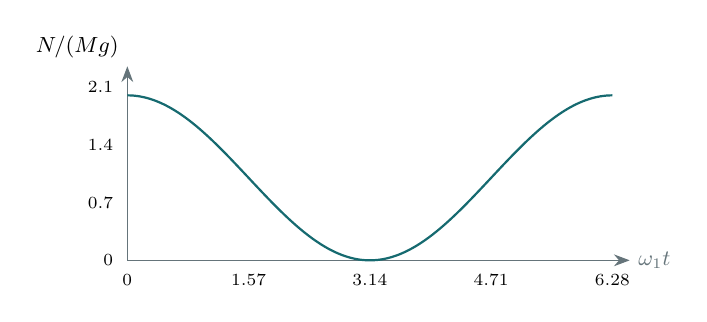
\begin{tikzpicture}[scale=.88,transform shape]
\draw[axis] (0,0.0000000)--(7.25,0.0000000) node[right] {$\omega_1t$};
\draw[axis] (0.0000000,0)--(0.0000000,2.8);
\node[above left] at (0.0000000,2.8) {$N/(Mg)$};
\node[below,font=\scriptsize] at (0.0000000,-0.0800000) {$0$};
\node[below,font=\scriptsize] at (1.7500000,-0.0800000) {$1.57$};
\node[below,font=\scriptsize] at (3.5000000,-0.0800000) {$3.14$};
\node[below,font=\scriptsize] at (5.2500000,-0.0800000) {$4.71$};
\node[below,font=\scriptsize] at (7.0000000,-0.0800000) {$6.28$};
\node[left,font=\scriptsize] at (-0.0800000,0.0000000) {$0$};
\node[left,font=\scriptsize] at (-0.0800000,0.8333333) {$0.7$};
\node[left,font=\scriptsize] at (-0.0800000,1.6666667) {$1.4$};
\node[left,font=\scriptsize] at (-0.0800000,2.5000000) {$2.1$};
\draw[thick,color=accent] plot coordinates {(0.0000000,2.3809524) (0.0291667,2.3805444) (0.0583333,2.3793209) (0.0875000,2.3772825) (0.1166667,2.3744308) (0.1458333,2.3707677) (0.1750000,2.3662956) (0.2041667,2.3610177) (0.2333333,2.3549376) (0.2625000,2.3480594) (0.2916667,2.3403879) (0.3208333,2.3319283) (0.3500000,2.3226863) (0.3791667,2.3126684) (0.4083333,2.3018815) (0.4375000,2.2903328) (0.4666667,2.2780303) (0.4958333,2.2649825) (0.5250000,2.2511982) (0.5541667,2.2366870) (0.5833333,2.2214588) (0.6125000,2.2055240) (0.6416667,2.1888935) (0.6708333,2.1715788) (0.7000000,2.1535917) (0.7291667,2.1349445) (0.7583333,2.1156500) (0.7875000,2.0957214) (0.8166667,2.0751724) (0.8458333,2.0540171) (0.8750000,2.0322700) (0.9041667,2.0099459) (0.9333333,1.9870602) (0.9625000,1.9636286) (0.9916667,1.9396671) (1.0208333,1.9151922) (1.0500000,1.8902205) (1.0791667,1.8647693) (1.1083333,1.8388560) (1.1375000,1.8124983) (1.1666667,1.7857143) (1.1958333,1.7585223) (1.2250000,1.7309411) (1.2541667,1.7029894) (1.2833333,1.6746865) (1.3125000,1.6460517) (1.3416667,1.6171047) (1.3708333,1.5878653) (1.4000000,1.5583536) (1.4291667,1.5285897) (1.4583333,1.4985941) (1.4875000,1.4683873) (1.5166667,1.4379901) (1.5458333,1.4074232) (1.5750000,1.3767077) (1.6041667,1.3458645) (1.6333333,1.3149148) (1.6625000,1.2838799) (1.6916667,1.2527809) (1.7208333,1.2216392) (1.7500000,1.1904762) (1.7791667,1.1593132) (1.8083333,1.1281715) (1.8375000,1.0970725) (1.8666667,1.0660375) (1.8958333,1.0350879) (1.9250000,1.0042447) (1.9541667,0.9735291) (1.9833333,0.9429623) (2.0125000,0.9125650) (2.0416667,0.8823583) (2.0708333,0.8523627) (2.1000000,0.8225988) (2.1291667,0.7930871) (2.1583333,0.7638477) (2.1875000,0.7349007) (2.2166667,0.7062659) (2.2458333,0.6779630) (2.2750000,0.6500113) (2.3041667,0.6224300) (2.3333333,0.5952381) (2.3625000,0.5684541) (2.3916667,0.5420964) (2.4208333,0.5161831) (2.4500000,0.4907318) (2.4791667,0.4657602) (2.5083333,0.4412852) (2.5375000,0.4173238) (2.5666667,0.3938921) (2.5958333,0.3710065) (2.6250000,0.3486824) (2.6541667,0.3269353) (2.6833333,0.3057800) (2.7125000,0.2852310) (2.7416667,0.2653024) (2.7708333,0.2460079) (2.8000000,0.2273607) (2.8291667,0.2093736) (2.8583333,0.1920588) (2.8875000,0.1754284) (2.9166667,0.1594936) (2.9458333,0.1442653) (2.9750000,0.1297541) (3.0041667,0.1159699) (3.0333333,0.1029221) (3.0625000,0.0906196) (3.0916667,0.0790709) (3.1208333,0.0682839) (3.1500000,0.0582661) (3.1791667,0.0490241) (3.2083333,0.0405645) (3.2375000,0.0328930) (3.2666667,0.0260148) (3.2958333,0.0199346) (3.3250000,0.0146567) (3.3541667,0.0101847) (3.3833333,0.0065216) (3.4125000,0.0036698) (3.4416667,0.0016315) (3.4708333,0.0004079) (3.5000000,0.0000000) (3.5291667,0.0004079) (3.5583333,0.0016315) (3.5875000,0.0036698) (3.6166667,0.0065216) (3.6458333,0.0101847) (3.6750000,0.0146567) (3.7041667,0.0199346) (3.7333333,0.0260148) (3.7625000,0.0328930) (3.7916667,0.0405645) (3.8208333,0.0490241) (3.8500000,0.0582661) (3.8791667,0.0682839) (3.9083333,0.0790709) (3.9375000,0.0906196) (3.9666667,0.1029221) (3.9958333,0.1159699) (4.0250000,0.1297541) (4.0541667,0.1442653) (4.0833333,0.1594936) (4.1125000,0.1754284) (4.1416667,0.1920588) (4.1708333,0.2093736) (4.2000000,0.2273607) (4.2291667,0.2460079) (4.2583333,0.2653024) (4.2875000,0.2852310) (4.3166667,0.3057800) (4.3458333,0.3269353) (4.3750000,0.3486824) (4.4041667,0.3710065) (4.4333333,0.3938921) (4.4625000,0.4173238) (4.4916667,0.4412852) (4.5208333,0.4657602) (4.5500000,0.4907318) (4.5791667,0.5161831) (4.6083333,0.5420964) (4.6375000,0.5684541) (4.6666667,0.5952381) (4.6958333,0.6224300) (4.7250000,0.6500113) (4.7541667,0.6779630) (4.7833333,0.7062659) (4.8125000,0.7349007) (4.8416667,0.7638477) (4.8708333,0.7930871) (4.9000000,0.8225988) (4.9291667,0.8523627) (4.9583333,0.8823583) (4.9875000,0.9125650) (5.0166667,0.9429623) (5.0458333,0.9735291) (5.0750000,1.0042447) (5.1041667,1.0350879) (5.1333333,1.0660375) (5.1625000,1.0970725) (5.1916667,1.1281715) (5.2208333,1.1593132) (5.2500000,1.1904762) (5.2791667,1.2216392) (5.3083333,1.2527809) (5.3375000,1.2838799) (5.3666667,1.3149148) (5.3958333,1.3458645) (5.4250000,1.3767077) (5.4541667,1.4074232) (5.4833333,1.4379901) (5.5125000,1.4683873) (5.5416667,1.4985941) (5.5708333,1.5285897) (5.6000000,1.5583536) (5.6291667,1.5878653) (5.6583333,1.6171047) (5.6875000,1.6460517) (5.7166667,1.6746865) (5.7458333,1.7029894) (5.7750000,1.7309411) (5.8041667,1.7585223) (5.8333333,1.7857143) (5.8625000,1.8124983) (5.8916667,1.8388560) (5.9208333,1.8647693) (5.9500000,1.8902205) (5.9791667,1.9151922) (6.0083333,1.9396671) (6.0375000,1.9636286) (6.0666667,1.9870602) (6.0958333,2.0099459) (6.1250000,2.0322700) (6.1541667,2.0540171) (6.1833333,2.0751724) (6.2125000,2.0957214) (6.2416667,2.1156500) (6.2708333,2.1349445) (6.3000000,2.1535917) (6.3291667,2.1715788) (6.3583333,2.1888935) (6.3875000,2.2055240) (6.4166667,2.2214588) (6.4458333,2.2366870) (6.4750000,2.2511982) (6.5041667,2.2649825) (6.5333333,2.2780303) (6.5625000,2.2903328) (6.5916667,2.3018815) (6.6208333,2.3126684) (6.6500000,2.3226863) (6.6791667,2.3319283) (6.7083333,2.3403879) (6.7375000,2.3480594) (6.7666667,2.3549376) (6.7958333,2.3610177) (6.8250000,2.3662956) (6.8541667,2.3707677) (6.8833333,2.3744308) (6.9125000,2.3772825) (6.9416667,2.3793209) (6.9708333,2.3805444) (7.0000000,2.3809524)};
\end{tikzpicture}
\figcaption{变图综二.2V1\quad 临界振幅下的支持力只在最高点触及零}
\end{minipage}\end{center}
\item \textbf{把一次起落的总时间算出来。}取两质量相等，$k=10mg/R$。求离地前、飞行和完整周期的时间。记$\kappa=kR/(mg)$。有$\Omega=\sqrt{2\kappa g/R}$、$h=R/\kappa$，故
\[
t_*\sqrt{g/R}=2\chi_1/\sqrt{2\kappa},\qquad
t_{\rm leave}\sqrt{g/R}=\frac{\pi/2+\arcsin[2/\sqrt{4+2\chi_1^2}]}{\sqrt\kappa}.
\]
在图V2的$\kappa=10$处分别约为$2.01$和$0.593$，壳落下后再经过一个地面单程，故总周期约为$3.20\sqrt{R/g}$。
\begin{center}\begin{minipage}{.98\linewidth}\centering
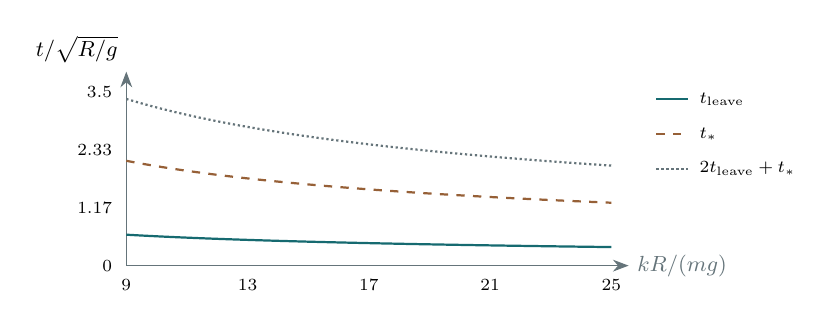
\begin{tikzpicture}[scale=.88,transform shape]
\draw[axis] (0,0.0000000)--(7.25,0.0000000) node[right] {$kR/(mg)$};
\draw[axis] (0.0000000,0)--(0.0000000,2.8);
\node[above left] at (0.0000000,2.8) {$t/\sqrt{R/g}$};
\node[below,font=\scriptsize] at (0.0000000,-0.0800000) {$9$};
\node[below,font=\scriptsize] at (1.7500000,-0.0800000) {$13$};
\node[below,font=\scriptsize] at (3.5000000,-0.0800000) {$17$};
\node[below,font=\scriptsize] at (5.2500000,-0.0800000) {$21$};
\node[below,font=\scriptsize] at (7.0000000,-0.0800000) {$25$};
\node[left,font=\scriptsize] at (-0.0800000,0.0000000) {$0$};
\node[left,font=\scriptsize] at (-0.0800000,0.8333333) {$1.17$};
\node[left,font=\scriptsize] at (-0.0800000,1.6666667) {$2.33$};
\node[left,font=\scriptsize] at (-0.0800000,2.5000000) {$3.5$};
\draw[thick,color=accent] plot coordinates {(0.0000000,0.4465981) (0.0291667,0.4449532) (0.0583333,0.4433263) (0.0875000,0.4417171) (0.1166667,0.4401253) (0.1458333,0.4385506) (0.1750000,0.4369927) (0.2041667,0.4354513) (0.2333333,0.4339261) (0.2625000,0.4324168) (0.2916667,0.4309231) (0.3208333,0.4294448) (0.3500000,0.4279816) (0.3791667,0.4265333) (0.4083333,0.4250995) (0.4375000,0.4236802) (0.4666667,0.4222749) (0.4958333,0.4208836) (0.5250000,0.4195059) (0.5541667,0.4181416) (0.5833333,0.4167906) (0.6125000,0.4154526) (0.6416667,0.4141274) (0.6708333,0.4128148) (0.7000000,0.4115146) (0.7291667,0.4102266) (0.7583333,0.4089506) (0.7875000,0.4076864) (0.8166667,0.4064339) (0.8458333,0.4051929) (0.8750000,0.4039632) (0.9041667,0.4027446) (0.9333333,0.4015370) (0.9625000,0.4003401) (0.9916667,0.3991539) (1.0208333,0.3979782) (1.0500000,0.3968128) (1.0791667,0.3956576) (1.1083333,0.3945125) (1.1375000,0.3933772) (1.1666667,0.3922516) (1.1958333,0.3911357) (1.2250000,0.3900292) (1.2541667,0.3889321) (1.2833333,0.3878442) (1.3125000,0.3867653) (1.3416667,0.3856954) (1.3708333,0.3846344) (1.4000000,0.3835820) (1.4291667,0.3825382) (1.4583333,0.3815030) (1.4875000,0.3804760) (1.5166667,0.3794573) (1.5458333,0.3784468) (1.5750000,0.3774443) (1.6041667,0.3764497) (1.6333333,0.3754629) (1.6625000,0.3744839) (1.6916667,0.3735125) (1.7208333,0.3725486) (1.7500000,0.3715921) (1.7791667,0.3706429) (1.8083333,0.3697010) (1.8375000,0.3687663) (1.8666667,0.3678385) (1.8958333,0.3669178) (1.9250000,0.3660039) (1.9541667,0.3650968) (1.9833333,0.3641965) (2.0125000,0.3633027) (2.0416667,0.3624156) (2.0708333,0.3615348) (2.1000000,0.3606605) (2.1291667,0.3597925) (2.1583333,0.3589307) (2.1875000,0.3580751) (2.2166667,0.3572256) (2.2458333,0.3563821) (2.2750000,0.3555445) (2.3041667,0.3547128) (2.3333333,0.3538869) (2.3625000,0.3530668) (2.3916667,0.3522524) (2.4208333,0.3514435) (2.4500000,0.3506402) (2.4791667,0.3498424) (2.5083333,0.3490500) (2.5375000,0.3482630) (2.5666667,0.3474812) (2.5958333,0.3467047) (2.6250000,0.3459334) (2.6541667,0.3451672) (2.6833333,0.3444061) (2.7125000,0.3436500) (2.7416667,0.3428988) (2.7708333,0.3421526) (2.8000000,0.3414112) (2.8291667,0.3406746) (2.8583333,0.3399428) (2.8875000,0.3392156) (2.9166667,0.3384931) (2.9458333,0.3377752) (2.9750000,0.3370618) (3.0041667,0.3363530) (3.0333333,0.3356486) (3.0625000,0.3349486) (3.0916667,0.3342529) (3.1208333,0.3335616) (3.1500000,0.3328746) (3.1791667,0.3321918) (3.2083333,0.3315131) (3.2375000,0.3308386) (3.2666667,0.3301682) (3.2958333,0.3295019) (3.3250000,0.3288396) (3.3541667,0.3281812) (3.3833333,0.3275268) (3.4125000,0.3268763) (3.4416667,0.3262297) (3.4708333,0.3255869) (3.5000000,0.3249479) (3.5291667,0.3243126) (3.5583333,0.3236810) (3.5875000,0.3230531) (3.6166667,0.3224288) (3.6458333,0.3218082) (3.6750000,0.3211911) (3.7041667,0.3205776) (3.7333333,0.3199675) (3.7625000,0.3193609) (3.7916667,0.3187578) (3.8208333,0.3181581) (3.8500000,0.3175617) (3.8791667,0.3169687) (3.9083333,0.3163790) (3.9375000,0.3157926) (3.9666667,0.3152094) (3.9958333,0.3146294) (4.0250000,0.3140526) (4.0541667,0.3134790) (4.0833333,0.3129085) (4.1125000,0.3123412) (4.1416667,0.3117769) (4.1708333,0.3112156) (4.2000000,0.3106574) (4.2291667,0.3101021) (4.2583333,0.3095499) (4.2875000,0.3090005) (4.3166667,0.3084541) (4.3458333,0.3079106) (4.3750000,0.3073699) (4.4041667,0.3068321) (4.4333333,0.3062971) (4.4625000,0.3057648) (4.4916667,0.3052354) (4.5208333,0.3047086) (4.5500000,0.3041846) (4.5791667,0.3036633) (4.6083333,0.3031447) (4.6375000,0.3026287) (4.6666667,0.3021153) (4.6958333,0.3016046) (4.7250000,0.3010964) (4.7541667,0.3005908) (4.7833333,0.3000877) (4.8125000,0.2995871) (4.8416667,0.2990891) (4.8708333,0.2985935) (4.9000000,0.2981003) (4.9291667,0.2976096) (4.9583333,0.2971213) (4.9875000,0.2966355) (5.0166667,0.2961519) (5.0458333,0.2956708) (5.0750000,0.2951920) (5.1041667,0.2947155) (5.1333333,0.2942413) (5.1625000,0.2937693) (5.1916667,0.2932997) (5.2208333,0.2928323) (5.2500000,0.2923671) (5.2791667,0.2919041) (5.3083333,0.2914433) (5.3375000,0.2909847) (5.3666667,0.2905283) (5.3958333,0.2900740) (5.4250000,0.2896218) (5.4541667,0.2891717) (5.4833333,0.2887237) (5.5125000,0.2882778) (5.5416667,0.2878340) (5.5708333,0.2873922) (5.6000000,0.2869524) (5.6291667,0.2865147) (5.6583333,0.2860789) (5.6875000,0.2856451) (5.7166667,0.2852133) (5.7458333,0.2847834) (5.7750000,0.2843555) (5.8041667,0.2839295) (5.8333333,0.2835054) (5.8625000,0.2830832) (5.8916667,0.2826629) (5.9208333,0.2822445) (5.9500000,0.2818279) (5.9791667,0.2814131) (6.0083333,0.2810002) (6.0375000,0.2805890) (6.0666667,0.2801797) (6.0958333,0.2797722) (6.1250000,0.2793664) (6.1541667,0.2789624) (6.1833333,0.2785602) (6.2125000,0.2781597) (6.2416667,0.2777609) (6.2708333,0.2773638) (6.3000000,0.2769684) (6.3291667,0.2765747) (6.3583333,0.2761827) (6.3875000,0.2757923) (6.4166667,0.2754036) (6.4458333,0.2750165) (6.4750000,0.2746311) (6.5041667,0.2742472) (6.5333333,0.2738650) (6.5625000,0.2734844) (6.5916667,0.2731053) (6.6208333,0.2727278) (6.6500000,0.2723519) (6.6791667,0.2719776) (6.7083333,0.2716047) (6.7375000,0.2712334) (6.7666667,0.2708637) (6.7958333,0.2704954) (6.8250000,0.2701286) (6.8541667,0.2697633) (6.8833333,0.2693995) (6.9125000,0.2690372) (6.9416667,0.2686763) (6.9708333,0.2683169) (7.0000000,0.2679589)};
\draw[thick,color=accent] (7.65,2.4)--(8.1,2.4);\node[right,font=\scriptsize] at (8.15,2.4) {$t_{\rm leave}$};
\draw[thick,dashed,color=warm] plot coordinates {(0.0000000,1.5130097) (0.0291667,1.5074369) (0.0583333,1.5019252) (0.0875000,1.4964735) (0.1166667,1.4910808) (0.1458333,1.4857460) (0.1750000,1.4804680) (0.2041667,1.4752459) (0.2333333,1.4700786) (0.2625000,1.4649653) (0.2916667,1.4599050) (0.3208333,1.4548967) (0.3500000,1.4499396) (0.3791667,1.4450329) (0.4083333,1.4401756) (0.4375000,1.4353670) (0.4666667,1.4306062) (0.4958333,1.4258925) (0.5250000,1.4212251) (0.5541667,1.4166032) (0.5833333,1.4120261) (0.6125000,1.4074931) (0.6416667,1.4030035) (0.6708333,1.3985566) (0.7000000,1.3941517) (0.7291667,1.3897881) (0.7583333,1.3854653) (0.7875000,1.3811825) (0.8166667,1.3769393) (0.8458333,1.3727349) (0.8750000,1.3685687) (0.9041667,1.3644403) (0.9333333,1.3603490) (0.9625000,1.3562943) (0.9916667,1.3522757) (1.0208333,1.3482925) (1.0500000,1.3443444) (1.0791667,1.3404307) (1.1083333,1.3365510) (1.1375000,1.3327048) (1.1666667,1.3288916) (1.1958333,1.3251110) (1.2250000,1.3213624) (1.2541667,1.3176455) (1.2833333,1.3139598) (1.3125000,1.3103048) (1.3416667,1.3066802) (1.3708333,1.3030854) (1.4000000,1.2995202) (1.4291667,1.2959841) (1.4583333,1.2924767) (1.4875000,1.2889976) (1.5166667,1.2855465) (1.5458333,1.2821229) (1.5750000,1.2787266) (1.6041667,1.2753570) (1.6333333,1.2720140) (1.6625000,1.2686972) (1.6916667,1.2654061) (1.7208333,1.2621406) (1.7500000,1.2589001) (1.7791667,1.2556846) (1.8083333,1.2524935) (1.8375000,1.2493266) (1.8666667,1.2461836) (1.8958333,1.2430643) (1.9250000,1.2399682) (1.9541667,1.2368952) (1.9833333,1.2338449) (2.0125000,1.2308170) (2.0416667,1.2278114) (2.0708333,1.2248276) (2.1000000,1.2218655) (2.1291667,1.2189248) (2.1583333,1.2160052) (2.1875000,1.2131065) (2.2166667,1.2102285) (2.2458333,1.2073708) (2.2750000,1.2045332) (2.3041667,1.2017156) (2.3333333,1.1989177) (2.3625000,1.1961392) (2.3916667,1.1933799) (2.4208333,1.1906396) (2.4500000,1.1879182) (2.4791667,1.1852153) (2.5083333,1.1825308) (2.5375000,1.1798644) (2.5666667,1.1772160) (2.5958333,1.1745853) (2.6250000,1.1719722) (2.6541667,1.1693765) (2.6833333,1.1667980) (2.7125000,1.1642364) (2.7416667,1.1616916) (2.7708333,1.1591634) (2.8000000,1.1566517) (2.8291667,1.1541562) (2.8583333,1.1516768) (2.8875000,1.1492133) (2.9166667,1.1467656) (2.9458333,1.1443334) (2.9750000,1.1419167) (3.0041667,1.1395152) (3.0333333,1.1371287) (3.0625000,1.1347572) (3.0916667,1.1324005) (3.1208333,1.1300584) (3.1500000,1.1277308) (3.1791667,1.1254175) (3.2083333,1.1231184) (3.2375000,1.1208333) (3.2666667,1.1185621) (3.2958333,1.1163047) (3.3250000,1.1140609) (3.3541667,1.1118305) (3.3833333,1.1096135) (3.4125000,1.1074097) (3.4416667,1.1052190) (3.4708333,1.1030412) (3.5000000,1.1008762) (3.5291667,1.0987240) (3.5583333,1.0965843) (3.5875000,1.0944571) (3.6166667,1.0923422) (3.6458333,1.0902395) (3.6750000,1.0881489) (3.7041667,1.0860703) (3.7333333,1.0840036) (3.7625000,1.0819486) (3.7916667,1.0799052) (3.8208333,1.0778734) (3.8500000,1.0758531) (3.8791667,1.0738440) (3.9083333,1.0718461) (3.9375000,1.0698594) (3.9666667,1.0678837) (3.9958333,1.0659188) (4.0250000,1.0639648) (4.0541667,1.0620215) (4.0833333,1.0600888) (4.1125000,1.0581666) (4.1416667,1.0562548) (4.1708333,1.0543534) (4.2000000,1.0524621) (4.2291667,1.0505811) (4.2583333,1.0487100) (4.2875000,1.0468490) (4.3166667,1.0449978) (4.3458333,1.0431564) (4.3750000,1.0413247) (4.4041667,1.0395026) (4.4333333,1.0376900) (4.4625000,1.0358869) (4.4916667,1.0340932) (4.5208333,1.0323087) (4.5500000,1.0305334) (4.5791667,1.0287673) (4.6083333,1.0270102) (4.6375000,1.0252621) (4.6666667,1.0235229) (4.6958333,1.0217925) (4.7250000,1.0200709) (4.7541667,1.0183579) (4.7833333,1.0166536) (4.8125000,1.0149577) (4.8416667,1.0132704) (4.8708333,1.0115914) (4.9000000,1.0099207) (4.9291667,1.0082583) (4.9583333,1.0066040) (4.9875000,1.0049579) (5.0166667,1.0033198) (5.0458333,1.0016897) (5.0750000,1.0000676) (5.1041667,0.9984533) (5.1333333,0.9968467) (5.1625000,0.9952479) (5.1916667,0.9936568) (5.2208333,0.9920733) (5.2500000,0.9904973) (5.2791667,0.9889288) (5.3083333,0.9873678) (5.3375000,0.9858141) (5.3666667,0.9842677) (5.3958333,0.9827286) (5.4250000,0.9811967) (5.4541667,0.9796719) (5.4833333,0.9781542) (5.5125000,0.9766435) (5.5416667,0.9751399) (5.5708333,0.9736431) (5.6000000,0.9721532) (5.6291667,0.9706701) (5.6583333,0.9691938) (5.6875000,0.9677242) (5.7166667,0.9662613) (5.7458333,0.9648050) (5.7750000,0.9633553) (5.8041667,0.9619120) (5.8333333,0.9604753) (5.8625000,0.9590449) (5.8916667,0.9576209) (5.9208333,0.9562033) (5.9500000,0.9547919) (5.9791667,0.9533868) (6.0083333,0.9519878) (6.0375000,0.9505950) (6.0666667,0.9492083) (6.0958333,0.9478276) (6.1250000,0.9464530) (6.1541667,0.9450843) (6.1833333,0.9437215) (6.2125000,0.9423646) (6.2416667,0.9410135) (6.2708333,0.9396683) (6.3000000,0.9383288) (6.3291667,0.9369950) (6.3583333,0.9356668) (6.3875000,0.9343443) (6.4166667,0.9330274) (6.4458333,0.9317161) (6.4750000,0.9304102) (6.5041667,0.9291099) (6.5333333,0.9278149) (6.5625000,0.9265254) (6.5916667,0.9252412) (6.6208333,0.9239624) (6.6500000,0.9226889) (6.6791667,0.9214206) (6.7083333,0.9201575) (6.7375000,0.9188996) (6.7666667,0.9176468) (6.7958333,0.9163991) (6.8250000,0.9151566) (6.8541667,0.9139190) (6.8833333,0.9126865) (6.9125000,0.9114590) (6.9416667,0.9102363) (6.9708333,0.9090186) (7.0000000,0.9078058)};
\draw[thick,dashed,color=warm] (7.65,1.9)--(8.1,1.9);\node[right,font=\scriptsize] at (8.15,1.9) {$t_*$};
\draw[thick,densely dotted,color=muted] plot coordinates {(0.0000000,2.4062059) (0.0291667,2.3973432) (0.0583333,2.3885778) (0.0875000,2.3799078) (0.1166667,2.3713315) (0.1458333,2.3628473) (0.1750000,2.3544535) (0.2041667,2.3461485) (0.2333333,2.3379308) (0.2625000,2.3297988) (0.2916667,2.3217511) (0.3208333,2.3137863) (0.3500000,2.3059028) (0.3791667,2.2980994) (0.4083333,2.2903747) (0.4375000,2.2827273) (0.4666667,2.2751561) (0.4958333,2.2676597) (0.5250000,2.2602369) (0.5541667,2.2528865) (0.5833333,2.2456073) (0.6125000,2.2383983) (0.6416667,2.2312583) (0.6708333,2.2241861) (0.7000000,2.2171808) (0.7291667,2.2102412) (0.7583333,2.2033664) (0.7875000,2.1965554) (0.8166667,2.1898071) (0.8458333,2.1831207) (0.8750000,2.1764951) (0.9041667,2.1699295) (0.9333333,2.1634230) (0.9625000,2.1569746) (0.9916667,2.1505835) (1.0208333,2.1442490) (1.0500000,2.1379700) (1.0791667,2.1317459) (1.1083333,2.1255759) (1.1375000,2.1194591) (1.1666667,2.1133949) (1.1958333,2.1073823) (1.2250000,2.1014208) (1.2541667,2.0955097) (1.2833333,2.0896481) (1.3125000,2.0838354) (1.3416667,2.0780710) (1.3708333,2.0723542) (1.4000000,2.0666842) (1.4291667,2.0610606) (1.4583333,2.0554826) (1.4875000,2.0499497) (1.5166667,2.0444612) (1.5458333,2.0390165) (1.5750000,2.0336151) (1.6041667,2.0282565) (1.6333333,2.0229399) (1.6625000,2.0176650) (1.6916667,2.0124311) (1.7208333,2.0072377) (1.7500000,2.0020843) (1.7791667,1.9969704) (1.8083333,1.9918955) (1.8375000,1.9868591) (1.8666667,1.9818607) (1.8958333,1.9768999) (1.9250000,1.9719761) (1.9541667,1.9670889) (1.9833333,1.9622379) (2.0125000,1.9574225) (2.0416667,1.9526425) (2.0708333,1.9478973) (2.1000000,1.9431866) (2.1291667,1.9385098) (2.1583333,1.9338667) (2.1875000,1.9292567) (2.2166667,1.9246796) (2.2458333,1.9201349) (2.2750000,1.9156222) (2.3041667,1.9111412) (2.3333333,1.9066915) (2.3625000,1.9022728) (2.3916667,1.8978846) (2.4208333,1.8935267) (2.4500000,1.8891986) (2.4791667,1.8849001) (2.5083333,1.8806308) (2.5375000,1.8763903) (2.5666667,1.8721784) (2.5958333,1.8679948) (2.6250000,1.8638391) (2.6541667,1.8597110) (2.6833333,1.8556102) (2.7125000,1.8515364) (2.7416667,1.8474893) (2.7708333,1.8434686) (2.8000000,1.8394741) (2.8291667,1.8355054) (2.8583333,1.8315624) (2.8875000,1.8276446) (2.9166667,1.8237518) (2.9458333,1.8198838) (2.9750000,1.8160404) (3.0041667,1.8122211) (3.0333333,1.8084259) (3.0625000,1.8046544) (3.0916667,1.8009064) (3.1208333,1.7971817) (3.1500000,1.7934800) (3.1791667,1.7898010) (3.2083333,1.7861447) (3.2375000,1.7825106) (3.2666667,1.7788986) (3.2958333,1.7753085) (3.3250000,1.7717400) (3.3541667,1.7681930) (3.3833333,1.7646672) (3.4125000,1.7611624) (3.4416667,1.7576784) (3.4708333,1.7542150) (3.5000000,1.7507719) (3.5291667,1.7473491) (3.5583333,1.7439463) (3.5875000,1.7405633) (3.6166667,1.7371999) (3.6458333,1.7338559) (3.6750000,1.7305311) (3.7041667,1.7272254) (3.7333333,1.7239386) (3.7625000,1.7206705) (3.7916667,1.7174209) (3.8208333,1.7141896) (3.8500000,1.7109765) (3.8791667,1.7077814) (3.9083333,1.7046041) (3.9375000,1.7014445) (3.9666667,1.6983024) (3.9958333,1.6951777) (4.0250000,1.6920701) (4.0541667,1.6889795) (4.0833333,1.6859059) (4.1125000,1.6828489) (4.1416667,1.6798085) (4.1708333,1.6767846) (4.2000000,1.6737769) (4.2291667,1.6707853) (4.2583333,1.6678098) (4.2875000,1.6648500) (4.3166667,1.6619060) (4.3458333,1.6589775) (4.3750000,1.6560645) (4.4041667,1.6531667) (4.4333333,1.6502841) (4.4625000,1.6474166) (4.4916667,1.6445639) (4.5208333,1.6417260) (4.5500000,1.6389027) (4.5791667,1.6360940) (4.6083333,1.6332996) (4.6375000,1.6305195) (4.6666667,1.6277536) (4.6958333,1.6250017) (4.7250000,1.6222637) (4.7541667,1.6195395) (4.7833333,1.6168289) (4.8125000,1.6141320) (4.8416667,1.6114485) (4.8708333,1.6087783) (4.9000000,1.6061214) (4.9291667,1.6034775) (4.9583333,1.6008467) (4.9875000,1.5982288) (5.0166667,1.5956237) (5.0458333,1.5930313) (5.0750000,1.5904515) (5.1041667,1.5878842) (5.1333333,1.5853293) (5.1625000,1.5827866) (5.1916667,1.5802562) (5.2208333,1.5777379) (5.2500000,1.5752315) (5.2791667,1.5727371) (5.3083333,1.5702545) (5.3375000,1.5677836) (5.3666667,1.5653243) (5.3958333,1.5628766) (5.4250000,1.5604403) (5.4541667,1.5580154) (5.4833333,1.5556017) (5.5125000,1.5531992) (5.5416667,1.5508078) (5.5708333,1.5484275) (5.6000000,1.5460580) (5.6291667,1.5436994) (5.6583333,1.5413516) (5.6875000,1.5390145) (5.7166667,1.5366879) (5.7458333,1.5343719) (5.7750000,1.5320663) (5.8041667,1.5297710) (5.8333333,1.5274861) (5.8625000,1.5252114) (5.8916667,1.5229468) (5.9208333,1.5206922) (5.9500000,1.5184476) (5.9791667,1.5162130) (6.0083333,1.5139882) (6.0375000,1.5117731) (6.0666667,1.5095678) (6.0958333,1.5073720) (6.1250000,1.5051858) (6.1541667,1.5030091) (6.1833333,1.5008419) (6.2125000,1.4986839) (6.2416667,1.4965353) (6.2708333,1.4943958) (6.3000000,1.4922655) (6.3291667,1.4901443) (6.3583333,1.4880322) (6.3875000,1.4859289) (6.4166667,1.4838346) (6.4458333,1.4817491) (6.4750000,1.4796724) (6.5041667,1.4776043) (6.5333333,1.4755450) (6.5625000,1.4734942) (6.5916667,1.4714519) (6.6208333,1.4694181) (6.6500000,1.4673927) (6.6791667,1.4653757) (6.7083333,1.4633669) (6.7375000,1.4613664) (6.7666667,1.4593741) (6.7958333,1.4573899) (6.8250000,1.4554138) (6.8541667,1.4534457) (6.8833333,1.4514855) (6.9125000,1.4495333) (6.9416667,1.4475889) (6.9708333,1.4456524) (7.0000000,1.4437235)};
\draw[thick,densely dotted,color=muted] (7.65,1.4)--(8.1,1.4);\node[right,font=\scriptsize] at (8.15,1.4) {$2t_{\rm leave}+t_*$};
\end{tikzpicture}
\figcaption{变图综二.2V2\quad 等质量时地面、飞行和周期的刚度关系}
\end{minipage}\end{center}
\item \textbf{让壳的质量远大于球。}固定$k,m_1$，增大$m_2$，求最小下拉量的渐近式。记$\eta=m_2/m_1$，由下拉量式得
\[
\frac{H_{\min}}h=\frac{\sqrt{(1+\eta)[1+\eta(1+\chi_1^2)]}}\eta
\longrightarrow\sqrt{1+\chi_1^2}.
\]
图V3实线趋近虚线，给$H_{\min}\sim(m_2g/k)\sqrt{1+\chi_1^2}$。同时相对振幅也为$h\sqrt{1+\chi_1^2}$。因此要在增重时保留壳内余量，可相应增大$R$或$k$，使$H_{\min}+m_1g/k<R$且相对振幅小于$R$。
\begin{center}\begin{minipage}{.98\linewidth}\centering
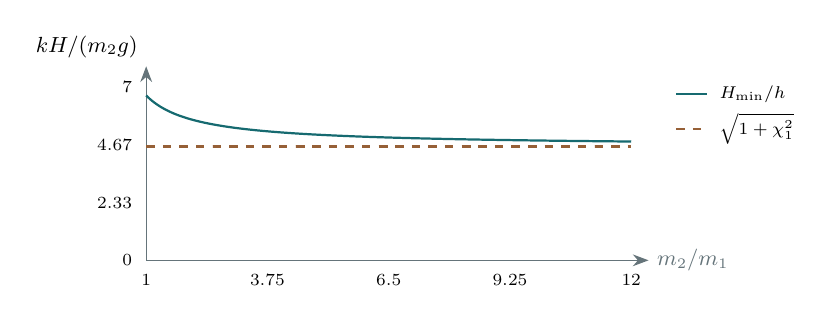
\begin{tikzpicture}[scale=.88,transform shape]
\draw[axis] (0,0.0000000)--(7.25,0.0000000) node[right] {$m_2/m_1$};
\draw[axis] (0.0000000,0)--(0.0000000,2.8);
\node[above left] at (0.0000000,2.8) {$kH/(m_2g)$};
\node[below,font=\scriptsize] at (0.0000000,-0.0800000) {$1$};
\node[below,font=\scriptsize] at (1.7500000,-0.0800000) {$3.75$};
\node[below,font=\scriptsize] at (3.5000000,-0.0800000) {$6.5$};
\node[below,font=\scriptsize] at (5.2500000,-0.0800000) {$9.25$};
\node[below,font=\scriptsize] at (7.0000000,-0.0800000) {$12$};
\node[left,font=\scriptsize] at (-0.0800000,0.0000000) {$0$};
\node[left,font=\scriptsize] at (-0.0800000,0.8333333) {$2.33$};
\node[left,font=\scriptsize] at (-0.0800000,1.6666667) {$4.67$};
\node[left,font=\scriptsize] at (-0.0800000,2.5000000) {$7$};
\draw[thick,color=accent] plot coordinates {(0.0000000,2.3792646) (0.0291667,2.3507279) (0.0583333,2.3243725) (0.0875000,2.2999533) (0.1166667,2.2772612) (0.1458333,2.2561164) (0.1750000,2.2363637) (0.2041667,2.2178680) (0.2333333,2.2005114) (0.2625000,2.1841904) (0.2916667,2.1688140) (0.3208333,2.1543014) (0.3500000,2.1405810) (0.3791667,2.1275889) (0.4083333,2.1152680) (0.4375000,2.1035671) (0.4666667,2.0924400) (0.4958333,2.0818452) (0.5250000,2.0717449) (0.5541667,2.0621051) (0.5833333,2.0528947) (0.6125000,2.0440853) (0.6416667,2.0356511) (0.6708333,2.0275685) (0.7000000,2.0198157) (0.7291667,2.0123729) (0.7583333,2.0052215) (0.7875000,1.9983449) (0.8166667,1.9917272) (0.8458333,1.9853541) (0.8750000,1.9792121) (0.9041667,1.9732888) (0.9333333,1.9675727) (0.9625000,1.9620530) (0.9916667,1.9567197) (1.0208333,1.9515635) (1.0500000,1.9465756) (1.0791667,1.9417479) (1.1083333,1.9370728) (1.1375000,1.9325431) (1.1666667,1.9281520) (1.1958333,1.9238933) (1.2250000,1.9197611) (1.2541667,1.9157498) (1.2833333,1.9118541) (1.3125000,1.9080690) (1.3416667,1.9043900) (1.3708333,1.9008126) (1.4000000,1.8973326) (1.4291667,1.8939460) (1.4583333,1.8906493) (1.4875000,1.8874387) (1.5166667,1.8843110) (1.5458333,1.8812630) (1.5750000,1.8782917) (1.6041667,1.8753942) (1.6333333,1.8725677) (1.6625000,1.8698098) (1.6916667,1.8671178) (1.7208333,1.8644895) (1.7500000,1.8619227) (1.7791667,1.8594151) (1.8083333,1.8569648) (1.8375000,1.8545698) (1.8666667,1.8522282) (1.8958333,1.8499384) (1.9250000,1.8476985) (1.9541667,1.8455069) (1.9833333,1.8433622) (2.0125000,1.8412628) (2.0416667,1.8392073) (2.0708333,1.8371943) (2.1000000,1.8352225) (2.1291667,1.8332907) (2.1583333,1.8313976) (2.1875000,1.8295421) (2.2166667,1.8277232) (2.2458333,1.8259396) (2.2750000,1.8241904) (2.3041667,1.8224746) (2.3333333,1.8207913) (2.3625000,1.8191395) (2.3916667,1.8175184) (2.4208333,1.8159271) (2.4500000,1.8143648) (2.4791667,1.8128307) (2.5083333,1.8113240) (2.5375000,1.8098440) (2.5666667,1.8083901) (2.5958333,1.8069615) (2.6250000,1.8055576) (2.6541667,1.8041777) (2.6833333,1.8028212) (2.7125000,1.8014876) (2.7416667,1.8001762) (2.7708333,1.7988865) (2.8000000,1.7976180) (2.8291667,1.7963702) (2.8583333,1.7951425) (2.8875000,1.7939345) (2.9166667,1.7927457) (2.9458333,1.7915756) (2.9750000,1.7904238) (3.0041667,1.7892899) (3.0333333,1.7881734) (3.0625000,1.7870740) (3.0916667,1.7859913) (3.1208333,1.7849249) (3.1500000,1.7838744) (3.1791667,1.7828395) (3.2083333,1.7818198) (3.2375000,1.7808150) (3.2666667,1.7798248) (3.2958333,1.7788488) (3.3250000,1.7778868) (3.3541667,1.7769384) (3.3833333,1.7760034) (3.4125000,1.7750815) (3.4416667,1.7741724) (3.4708333,1.7732758) (3.5000000,1.7723916) (3.5291667,1.7715193) (3.5583333,1.7706589) (3.5875000,1.7698100) (3.6166667,1.7689724) (3.6458333,1.7681459) (3.6750000,1.7673303) (3.7041667,1.7665254) (3.7333333,1.7657309) (3.7625000,1.7649467) (3.7916667,1.7641725) (3.8208333,1.7634082) (3.8500000,1.7626536) (3.8791667,1.7619084) (3.9083333,1.7611726) (3.9375000,1.7604459) (3.9666667,1.7597282) (3.9958333,1.7590193) (4.0250000,1.7583190) (4.0541667,1.7576273) (4.0833333,1.7569438) (4.1125000,1.7562686) (4.1416667,1.7556013) (4.1708333,1.7549420) (4.2000000,1.7542905) (4.2291667,1.7536465) (4.2583333,1.7530100) (4.2875000,1.7523809) (4.3166667,1.7517591) (4.3458333,1.7511443) (4.3750000,1.7505365) (4.4041667,1.7499356) (4.4333333,1.7493414) (4.4625000,1.7487539) (4.4916667,1.7481729) (4.5208333,1.7475983) (4.5500000,1.7470300) (4.5791667,1.7464679) (4.6083333,1.7459120) (4.6375000,1.7453620) (4.6666667,1.7448180) (4.6958333,1.7442798) (4.7250000,1.7437473) (4.7541667,1.7432204) (4.7833333,1.7426991) (4.8125000,1.7421832) (4.8416667,1.7416727) (4.8708333,1.7411675) (4.9000000,1.7406675) (4.9291667,1.7401726) (4.9583333,1.7396828) (4.9875000,1.7391979) (5.0166667,1.7387180) (5.0458333,1.7382428) (5.0750000,1.7377724) (5.1041667,1.7373067) (5.1333333,1.7368456) (5.1625000,1.7363890) (5.1916667,1.7359370) (5.2208333,1.7354893) (5.2500000,1.7350459) (5.2791667,1.7346069) (5.3083333,1.7341720) (5.3375000,1.7337414) (5.3666667,1.7333148) (5.3958333,1.7328922) (5.4250000,1.7324737) (5.4541667,1.7320591) (5.4833333,1.7316483) (5.5125000,1.7312414) (5.5416667,1.7308382) (5.5708333,1.7304387) (5.6000000,1.7300429) (5.6291667,1.7296508) (5.6583333,1.7292621) (5.6875000,1.7288770) (5.7166667,1.7284954) (5.7458333,1.7281172) (5.7750000,1.7277423) (5.8041667,1.7273708) (5.8333333,1.7270026) (5.8625000,1.7266376) (5.8916667,1.7262758) (5.9208333,1.7259172) (5.9500000,1.7255617) (5.9791667,1.7252093) (6.0083333,1.7248599) (6.0375000,1.7245135) (6.0666667,1.7241700) (6.0958333,1.7238295) (6.1250000,1.7234919) (6.1541667,1.7231571) (6.1833333,1.7228251) (6.2125000,1.7224959) (6.2416667,1.7221694) (6.2708333,1.7218457) (6.3000000,1.7215246) (6.3291667,1.7212062) (6.3583333,1.7208903) (6.3875000,1.7205771) (6.4166667,1.7202664) (6.4458333,1.7199582) (6.4750000,1.7196525) (6.5041667,1.7193492) (6.5333333,1.7190484) (6.5625000,1.7187499) (6.5916667,1.7184538) (6.6208333,1.7181601) (6.6500000,1.7178687) (6.6791667,1.7175796) (6.7083333,1.7172927) (6.7375000,1.7170080) (6.7666667,1.7167256) (6.7958333,1.7164453) (6.8250000,1.7161672) (6.8541667,1.7158912) (6.8833333,1.7156173) (6.9125000,1.7153455) (6.9416667,1.7150758) (6.9708333,1.7148081) (7.0000000,1.7145424)};
\draw[thick,color=accent] (7.65,2.4)--(8.1,2.4);\node[right,font=\scriptsize] at (8.15,2.4) {$H_{\min}/h$};
\draw[thick,dashed,color=warm] plot coordinates {(0.0000000,1.6440496) (0.0291667,1.6440496) (0.0583333,1.6440496) (0.0875000,1.6440496) (0.1166667,1.6440496) (0.1458333,1.6440496) (0.1750000,1.6440496) (0.2041667,1.6440496) (0.2333333,1.6440496) (0.2625000,1.6440496) (0.2916667,1.6440496) (0.3208333,1.6440496) (0.3500000,1.6440496) (0.3791667,1.6440496) (0.4083333,1.6440496) (0.4375000,1.6440496) (0.4666667,1.6440496) (0.4958333,1.6440496) (0.5250000,1.6440496) (0.5541667,1.6440496) (0.5833333,1.6440496) (0.6125000,1.6440496) (0.6416667,1.6440496) (0.6708333,1.6440496) (0.7000000,1.6440496) (0.7291667,1.6440496) (0.7583333,1.6440496) (0.7875000,1.6440496) (0.8166667,1.6440496) (0.8458333,1.6440496) (0.8750000,1.6440496) (0.9041667,1.6440496) (0.9333333,1.6440496) (0.9625000,1.6440496) (0.9916667,1.6440496) (1.0208333,1.6440496) (1.0500000,1.6440496) (1.0791667,1.6440496) (1.1083333,1.6440496) (1.1375000,1.6440496) (1.1666667,1.6440496) (1.1958333,1.6440496) (1.2250000,1.6440496) (1.2541667,1.6440496) (1.2833333,1.6440496) (1.3125000,1.6440496) (1.3416667,1.6440496) (1.3708333,1.6440496) (1.4000000,1.6440496) (1.4291667,1.6440496) (1.4583333,1.6440496) (1.4875000,1.6440496) (1.5166667,1.6440496) (1.5458333,1.6440496) (1.5750000,1.6440496) (1.6041667,1.6440496) (1.6333333,1.6440496) (1.6625000,1.6440496) (1.6916667,1.6440496) (1.7208333,1.6440496) (1.7500000,1.6440496) (1.7791667,1.6440496) (1.8083333,1.6440496) (1.8375000,1.6440496) (1.8666667,1.6440496) (1.8958333,1.6440496) (1.9250000,1.6440496) (1.9541667,1.6440496) (1.9833333,1.6440496) (2.0125000,1.6440496) (2.0416667,1.6440496) (2.0708333,1.6440496) (2.1000000,1.6440496) (2.1291667,1.6440496) (2.1583333,1.6440496) (2.1875000,1.6440496) (2.2166667,1.6440496) (2.2458333,1.6440496) (2.2750000,1.6440496) (2.3041667,1.6440496) (2.3333333,1.6440496) (2.3625000,1.6440496) (2.3916667,1.6440496) (2.4208333,1.6440496) (2.4500000,1.6440496) (2.4791667,1.6440496) (2.5083333,1.6440496) (2.5375000,1.6440496) (2.5666667,1.6440496) (2.5958333,1.6440496) (2.6250000,1.6440496) (2.6541667,1.6440496) (2.6833333,1.6440496) (2.7125000,1.6440496) (2.7416667,1.6440496) (2.7708333,1.6440496) (2.8000000,1.6440496) (2.8291667,1.6440496) (2.8583333,1.6440496) (2.8875000,1.6440496) (2.9166667,1.6440496) (2.9458333,1.6440496) (2.9750000,1.6440496) (3.0041667,1.6440496) (3.0333333,1.6440496) (3.0625000,1.6440496) (3.0916667,1.6440496) (3.1208333,1.6440496) (3.1500000,1.6440496) (3.1791667,1.6440496) (3.2083333,1.6440496) (3.2375000,1.6440496) (3.2666667,1.6440496) (3.2958333,1.6440496) (3.3250000,1.6440496) (3.3541667,1.6440496) (3.3833333,1.6440496) (3.4125000,1.6440496) (3.4416667,1.6440496) (3.4708333,1.6440496) (3.5000000,1.6440496) (3.5291667,1.6440496) (3.5583333,1.6440496) (3.5875000,1.6440496) (3.6166667,1.6440496) (3.6458333,1.6440496) (3.6750000,1.6440496) (3.7041667,1.6440496) (3.7333333,1.6440496) (3.7625000,1.6440496) (3.7916667,1.6440496) (3.8208333,1.6440496) (3.8500000,1.6440496) (3.8791667,1.6440496) (3.9083333,1.6440496) (3.9375000,1.6440496) (3.9666667,1.6440496) (3.9958333,1.6440496) (4.0250000,1.6440496) (4.0541667,1.6440496) (4.0833333,1.6440496) (4.1125000,1.6440496) (4.1416667,1.6440496) (4.1708333,1.6440496) (4.2000000,1.6440496) (4.2291667,1.6440496) (4.2583333,1.6440496) (4.2875000,1.6440496) (4.3166667,1.6440496) (4.3458333,1.6440496) (4.3750000,1.6440496) (4.4041667,1.6440496) (4.4333333,1.6440496) (4.4625000,1.6440496) (4.4916667,1.6440496) (4.5208333,1.6440496) (4.5500000,1.6440496) (4.5791667,1.6440496) (4.6083333,1.6440496) (4.6375000,1.6440496) (4.6666667,1.6440496) (4.6958333,1.6440496) (4.7250000,1.6440496) (4.7541667,1.6440496) (4.7833333,1.6440496) (4.8125000,1.6440496) (4.8416667,1.6440496) (4.8708333,1.6440496) (4.9000000,1.6440496) (4.9291667,1.6440496) (4.9583333,1.6440496) (4.9875000,1.6440496) (5.0166667,1.6440496) (5.0458333,1.6440496) (5.0750000,1.6440496) (5.1041667,1.6440496) (5.1333333,1.6440496) (5.1625000,1.6440496) (5.1916667,1.6440496) (5.2208333,1.6440496) (5.2500000,1.6440496) (5.2791667,1.6440496) (5.3083333,1.6440496) (5.3375000,1.6440496) (5.3666667,1.6440496) (5.3958333,1.6440496) (5.4250000,1.6440496) (5.4541667,1.6440496) (5.4833333,1.6440496) (5.5125000,1.6440496) (5.5416667,1.6440496) (5.5708333,1.6440496) (5.6000000,1.6440496) (5.6291667,1.6440496) (5.6583333,1.6440496) (5.6875000,1.6440496) (5.7166667,1.6440496) (5.7458333,1.6440496) (5.7750000,1.6440496) (5.8041667,1.6440496) (5.8333333,1.6440496) (5.8625000,1.6440496) (5.8916667,1.6440496) (5.9208333,1.6440496) (5.9500000,1.6440496) (5.9791667,1.6440496) (6.0083333,1.6440496) (6.0375000,1.6440496) (6.0666667,1.6440496) (6.0958333,1.6440496) (6.1250000,1.6440496) (6.1541667,1.6440496) (6.1833333,1.6440496) (6.2125000,1.6440496) (6.2416667,1.6440496) (6.2708333,1.6440496) (6.3000000,1.6440496) (6.3291667,1.6440496) (6.3583333,1.6440496) (6.3875000,1.6440496) (6.4166667,1.6440496) (6.4458333,1.6440496) (6.4750000,1.6440496) (6.5041667,1.6440496) (6.5333333,1.6440496) (6.5625000,1.6440496) (6.5916667,1.6440496) (6.6208333,1.6440496) (6.6500000,1.6440496) (6.6791667,1.6440496) (6.7083333,1.6440496) (6.7375000,1.6440496) (6.7666667,1.6440496) (6.7958333,1.6440496) (6.8250000,1.6440496) (6.8541667,1.6440496) (6.8833333,1.6440496) (6.9125000,1.6440496) (6.9416667,1.6440496) (6.9708333,1.6440496) (7.0000000,1.6440496)};
\draw[thick,dashed,color=warm] (7.65,1.9)--(8.1,1.9);\node[right,font=\scriptsize] at (8.15,1.9) {$\sqrt{1+\chi_1^2}$};
\end{tikzpicture}
\figcaption{变图综二.2V3\quad 壳质量占优时的下拉量与极限}
\end{minipage}\end{center}
\item \textbf{第二个相位根能否装进壳。}取两质量相等，比较$\kappa=10$时前两个根。第二根在$(2\pi,5\pi/2)$，$\chi_2=7.72525\ldots$。由
\[
H_n/R=\sqrt{4+2\chi_n^2}/\kappa,\qquad H/R<1-1/\kappa
\]
得到$H_2\simeq1.11R$，而图V4点线在$\kappa=10$只允许$H<0.9R$，所以下拉位置落在壳底以下。实线的$H_1\simeq0.666R$则在允许区间。
\begin{center}\begin{minipage}{.98\linewidth}\centering
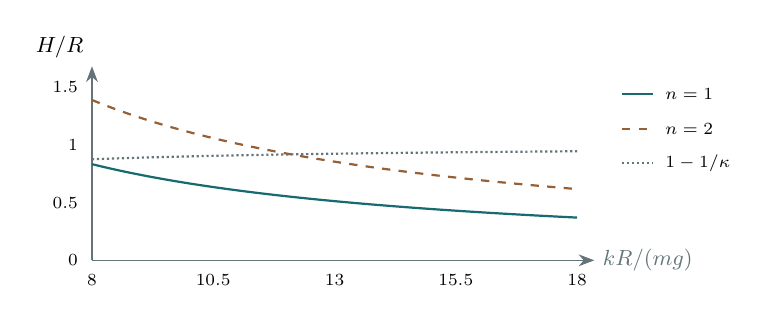
\begin{tikzpicture}[scale=.88,transform shape]
\draw[axis] (0,0.0000000)--(7.25,0.0000000) node[right] {$kR/(mg)$};
\draw[axis] (0.0000000,0)--(0.0000000,2.8);
\node[above left] at (0.0000000,2.8) {$H/R$};
\node[below,font=\scriptsize] at (0.0000000,-0.0800000) {$8$};
\node[below,font=\scriptsize] at (1.7500000,-0.0800000) {$10.5$};
\node[below,font=\scriptsize] at (3.5000000,-0.0800000) {$13$};
\node[below,font=\scriptsize] at (5.2500000,-0.0800000) {$15.5$};
\node[below,font=\scriptsize] at (7.0000000,-0.0800000) {$18$};
\node[left,font=\scriptsize] at (-0.0800000,0.0000000) {$0$};
\node[left,font=\scriptsize] at (-0.0800000,0.8333333) {$0.5$};
\node[left,font=\scriptsize] at (-0.0800000,1.6666667) {$1$};
\node[left,font=\scriptsize] at (-0.0800000,2.5000000) {$1.5$};
\draw[thick,color=accent] plot coordinates {(0.0000000,1.3879044) (0.0291667,1.3807131) (0.0583333,1.3735961) (0.0875000,1.3665520) (0.1166667,1.3595798) (0.1458333,1.3526784) (0.1750000,1.3458467) (0.2041667,1.3390836) (0.2333333,1.3323882) (0.2625000,1.3257594) (0.2916667,1.3191962) (0.3208333,1.3126977) (0.3500000,1.3062629) (0.3791667,1.2998909) (0.4083333,1.2935808) (0.4375000,1.2873316) (0.4666667,1.2811425) (0.4958333,1.2750126) (0.5250000,1.2689411) (0.5541667,1.2629272) (0.5833333,1.2569700) (0.6125000,1.2510687) (0.6416667,1.2452226) (0.6708333,1.2394309) (0.7000000,1.2336928) (0.7291667,1.2280075) (0.7583333,1.2223745) (0.7875000,1.2167929) (0.8166667,1.2112620) (0.8458333,1.2057812) (0.8750000,1.2003497) (0.9041667,1.1949670) (0.9333333,1.1896323) (0.9625000,1.1843451) (0.9916667,1.1791046) (1.0208333,1.1739103) (1.0500000,1.1687616) (1.0791667,1.1636578) (1.1083333,1.1585984) (1.1375000,1.1535828) (1.1666667,1.1486105) (1.1958333,1.1436808) (1.2250000,1.1387933) (1.2541667,1.1339474) (1.2833333,1.1291425) (1.3125000,1.1243782) (1.3416667,1.1196539) (1.3708333,1.1149692) (1.4000000,1.1103235) (1.4291667,1.1057163) (1.4583333,1.1011473) (1.4875000,1.0966158) (1.5166667,1.0921215) (1.5458333,1.0876638) (1.5750000,1.0832424) (1.6041667,1.0788568) (1.6333333,1.0745066) (1.6625000,1.0701913) (1.6916667,1.0659106) (1.7208333,1.0616639) (1.7500000,1.0574509) (1.7791667,1.0532713) (1.8083333,1.0491246) (1.8375000,1.0450103) (1.8666667,1.0409283) (1.8958333,1.0368780) (1.9250000,1.0328591) (1.9541667,1.0288712) (1.9833333,1.0249140) (2.0125000,1.0209871) (2.0416667,1.0170902) (2.0708333,1.0132230) (2.1000000,1.0093850) (2.1291667,1.0055760) (2.1583333,1.0017956) (2.1875000,0.9980436) (2.2166667,0.9943195) (2.2458333,0.9906232) (2.2750000,0.9869542) (2.3041667,0.9833123) (2.3333333,0.9796972) (2.3625000,0.9761086) (2.3916667,0.9725461) (2.4208333,0.9690096) (2.4500000,0.9654987) (2.4791667,0.9620131) (2.5083333,0.9585527) (2.5375000,0.9551170) (2.5666667,0.9517058) (2.5958333,0.9483190) (2.6250000,0.9449562) (2.6541667,0.9416171) (2.6833333,0.9383015) (2.7125000,0.9350093) (2.7416667,0.9317400) (2.7708333,0.9284935) (2.8000000,0.9252696) (2.8291667,0.9220680) (2.8583333,0.9188884) (2.8875000,0.9157307) (2.9166667,0.9125946) (2.9458333,0.9094800) (2.9750000,0.9063865) (3.0041667,0.9033140) (3.0333333,0.9002623) (3.0625000,0.8972311) (3.0916667,0.8942203) (3.1208333,0.8912296) (3.1500000,0.8882588) (3.1791667,0.8853078) (3.2083333,0.8823763) (3.2375000,0.8794642) (3.2666667,0.8765712) (3.2958333,0.8736972) (3.3250000,0.8708420) (3.3541667,0.8680053) (3.3833333,0.8651871) (3.4125000,0.8623872) (3.4416667,0.8596053) (3.4708333,0.8568413) (3.5000000,0.8540950) (3.5291667,0.8513663) (3.5583333,0.8486549) (3.5875000,0.8459608) (3.6166667,0.8432837) (3.6458333,0.8406235) (3.6750000,0.8379800) (3.7041667,0.8353531) (3.7333333,0.8327426) (3.7625000,0.8301484) (3.7916667,0.8275703) (3.8208333,0.8250082) (3.8500000,0.8224618) (3.8791667,0.8199312) (3.9083333,0.8174161) (3.9375000,0.8149163) (3.9666667,0.8124318) (3.9958333,0.8099624) (4.0250000,0.8075080) (4.0541667,0.8050684) (4.0833333,0.8026435) (4.1125000,0.8002331) (4.1416667,0.7978372) (4.1708333,0.7954556) (4.2000000,0.7930882) (4.2291667,0.7907348) (4.2583333,0.7883954) (4.2875000,0.7860697) (4.3166667,0.7837578) (4.3458333,0.7814593) (4.3750000,0.7791744) (4.4041667,0.7769027) (4.4333333,0.7746443) (4.4625000,0.7723989) (4.4916667,0.7701666) (4.5208333,0.7679471) (4.5500000,0.7657403) (4.5791667,0.7635462) (4.6083333,0.7613647) (4.6375000,0.7591955) (4.6666667,0.7570387) (4.6958333,0.7548942) (4.7250000,0.7527617) (4.7541667,0.7506412) (4.7833333,0.7485327) (4.8125000,0.7464360) (4.8416667,0.7443509) (4.8708333,0.7422775) (4.9000000,0.7402157) (4.9291667,0.7381652) (4.9583333,0.7361261) (4.9875000,0.7340982) (5.0166667,0.7320814) (5.0458333,0.7300757) (5.0750000,0.7280810) (5.1041667,0.7260971) (5.1333333,0.7241240) (5.1625000,0.7221616) (5.1916667,0.7202098) (5.2208333,0.7182686) (5.2500000,0.7163377) (5.2791667,0.7144173) (5.3083333,0.7125071) (5.3375000,0.7106070) (5.3666667,0.7087171) (5.3958333,0.7068372) (5.4250000,0.7049673) (5.4541667,0.7031072) (5.4833333,0.7012569) (5.5125000,0.6994164) (5.5416667,0.6975854) (5.5708333,0.6957641) (5.6000000,0.6939522) (5.6291667,0.6921497) (5.6583333,0.6903566) (5.6875000,0.6885727) (5.7166667,0.6867980) (5.7458333,0.6850325) (5.7750000,0.6832760) (5.8041667,0.6815285) (5.8333333,0.6797899) (5.8625000,0.6780601) (5.8916667,0.6763392) (5.9208333,0.6746269) (5.9500000,0.6729233) (5.9791667,0.6712283) (6.0083333,0.6695418) (6.0375000,0.6678638) (6.0666667,0.6661941) (6.0958333,0.6645328) (6.1250000,0.6628797) (6.1541667,0.6612348) (6.1833333,0.6595981) (6.2125000,0.6579695) (6.2416667,0.6563489) (6.2708333,0.6547362) (6.3000000,0.6531315) (6.3291667,0.6515346) (6.3583333,0.6499455) (6.3875000,0.6483641) (6.4166667,0.6467904) (6.4458333,0.6452243) (6.4750000,0.6436658) (6.5041667,0.6421148) (6.5333333,0.6405712) (6.5625000,0.6390351) (6.5916667,0.6375063) (6.6208333,0.6359848) (6.6500000,0.6344706) (6.6791667,0.6329635) (6.7083333,0.6314636) (6.7375000,0.6299708) (6.7666667,0.6284850) (6.7958333,0.6270062) (6.8250000,0.6255344) (6.8541667,0.6240694) (6.8833333,0.6226113) (6.9125000,0.6211600) (6.9416667,0.6197154) (6.9708333,0.6182776) (7.0000000,0.6168464)};
\draw[thick,color=accent] (7.65,2.4)--(8.1,2.4);\node[right,font=\scriptsize] at (8.15,2.4) {$n=1$};
\draw[thick,dashed,color=warm] plot coordinates {(0.0000000,2.3138981) (0.0291667,2.3019090) (0.0583333,2.2900435) (0.0875000,2.2782997) (0.1166667,2.2666757) (0.1458333,2.2551698) (0.1750000,2.2437800) (0.2041667,2.2325047) (0.2333333,2.2213422) (0.2625000,2.2102908) (0.2916667,2.1993487) (0.3208333,2.1885145) (0.3500000,2.1777865) (0.3791667,2.1671631) (0.4083333,2.1566429) (0.4375000,2.1462244) (0.4666667,2.1359060) (0.4958333,2.1256863) (0.5250000,2.1155640) (0.5541667,2.1055377) (0.5833333,2.0956059) (0.6125000,2.0857673) (0.6416667,2.0760208) (0.6708333,2.0663649) (0.7000000,2.0567984) (0.7291667,2.0473200) (0.7583333,2.0379286) (0.7875000,2.0286230) (0.8166667,2.0194020) (0.8458333,2.0102645) (0.8750000,2.0012092) (0.9041667,1.9922352) (0.9333333,1.9833413) (0.9625000,1.9745264) (0.9916667,1.9657896) (1.0208333,1.9571297) (1.0500000,1.9485458) (1.0791667,1.9400369) (1.1083333,1.9316019) (1.1375000,1.9232400) (1.1666667,1.9149502) (1.1958333,1.9067315) (1.2250000,1.8985831) (1.2541667,1.8905040) (1.2833333,1.8824934) (1.3125000,1.8745504) (1.3416667,1.8666741) (1.3708333,1.8588638) (1.4000000,1.8511185) (1.4291667,1.8434375) (1.4583333,1.8358200) (1.4875000,1.8282652) (1.5166667,1.8207723) (1.5458333,1.8133406) (1.5750000,1.8059693) (1.6041667,1.7986577) (1.6333333,1.7914050) (1.6625000,1.7842106) (1.6916667,1.7770738) (1.7208333,1.7699938) (1.7500000,1.7629700) (1.7791667,1.7560018) (1.8083333,1.7490884) (1.8375000,1.7422292) (1.8666667,1.7354236) (1.8958333,1.7286710) (1.9250000,1.7219707) (1.9541667,1.7153222) (1.9833333,1.7087248) (2.0125000,1.7021779) (2.0416667,1.6956811) (2.0708333,1.6892336) (2.1000000,1.6828350) (2.1291667,1.6764847) (2.1583333,1.6701821) (2.1875000,1.6639268) (2.2166667,1.6577181) (2.2458333,1.6515556) (2.2750000,1.6454387) (2.3041667,1.6393670) (2.3333333,1.6333399) (2.3625000,1.6273569) (2.3916667,1.6214177) (2.4208333,1.6155216) (2.4500000,1.6096683) (2.4791667,1.6038572) (2.5083333,1.5980879) (2.5375000,1.5923600) (2.5666667,1.5866730) (2.5958333,1.5810265) (2.6250000,1.5754200) (2.6541667,1.5698532) (2.6833333,1.5643255) (2.7125000,1.5588366) (2.7416667,1.5533862) (2.7708333,1.5479737) (2.8000000,1.5425988) (2.8291667,1.5372611) (2.8583333,1.5319602) (2.8875000,1.5266957) (2.9166667,1.5214673) (2.9458333,1.5162746) (2.9750000,1.5111172) (3.0041667,1.5059947) (3.0333333,1.5009069) (3.0625000,1.4958533) (3.0916667,1.4908337) (3.1208333,1.4858476) (3.1500000,1.4808948) (3.1791667,1.4759749) (3.2083333,1.4710876) (3.2375000,1.4662325) (3.2666667,1.4614094) (3.2958333,1.4566179) (3.3250000,1.4518577) (3.3541667,1.4471285) (3.3833333,1.4424300) (3.4125000,1.4377620) (3.4416667,1.4331240) (3.4708333,1.4285159) (3.5000000,1.4239373) (3.5291667,1.4193880) (3.5583333,1.4148677) (3.5875000,1.4103760) (3.6166667,1.4059128) (3.6458333,1.4014777) (3.6750000,1.3970706) (3.7041667,1.3926910) (3.7333333,1.3883389) (3.7625000,1.3840138) (3.7916667,1.3797157) (3.8208333,1.3754441) (3.8500000,1.3711989) (3.8791667,1.3669798) (3.9083333,1.3627866) (3.9375000,1.3586191) (3.9666667,1.3544770) (3.9958333,1.3503600) (4.0250000,1.3462680) (4.0541667,1.3422007) (4.0833333,1.3381580) (4.1125000,1.3341395) (4.1416667,1.3301450) (4.1708333,1.3261745) (4.2000000,1.3222275) (4.2291667,1.3183040) (4.2583333,1.3144037) (4.2875000,1.3105264) (4.3166667,1.3066719) (4.3458333,1.3028400) (4.3750000,1.2990305) (4.4041667,1.2952433) (4.4333333,1.2914780) (4.4625000,1.2877346) (4.4916667,1.2840128) (4.5208333,1.2803125) (4.5500000,1.2766335) (4.5791667,1.2729755) (4.6083333,1.2693384) (4.6375000,1.2657221) (4.6666667,1.2621263) (4.6958333,1.2585508) (4.7250000,1.2549956) (4.7541667,1.2514604) (4.7833333,1.2479451) (4.8125000,1.2444494) (4.8416667,1.2409733) (4.8708333,1.2375166) (4.9000000,1.2340790) (4.9291667,1.2306605) (4.9583333,1.2272609) (4.9875000,1.2238800) (5.0166667,1.2205177) (5.0458333,1.2171738) (5.0750000,1.2138482) (5.1041667,1.2105407) (5.1333333,1.2072512) (5.1625000,1.2039795) (5.1916667,1.2007255) (5.2208333,1.1974891) (5.2500000,1.1942700) (5.2791667,1.1910682) (5.3083333,1.1878835) (5.3375000,1.1847159) (5.3666667,1.1815650) (5.3958333,1.1784309) (5.4250000,1.1753133) (5.4541667,1.1722123) (5.4833333,1.1691275) (5.5125000,1.1660589) (5.5416667,1.1630064) (5.5708333,1.1599698) (5.6000000,1.1569491) (5.6291667,1.1539440) (5.6583333,1.1509545) (5.6875000,1.1479805) (5.7166667,1.1450218) (5.7458333,1.1420783) (5.7750000,1.1391499) (5.8041667,1.1362364) (5.8333333,1.1333379) (5.8625000,1.1304541) (5.8916667,1.1275849) (5.9208333,1.1247302) (5.9500000,1.1218900) (5.9791667,1.1190641) (6.0083333,1.1162524) (6.0375000,1.1134547) (6.0666667,1.1106711) (6.0958333,1.1079014) (6.1250000,1.1051454) (6.1541667,1.1024031) (6.1833333,1.0996744) (6.2125000,1.0969591) (6.2416667,1.0942573) (6.2708333,1.0915687) (6.3000000,1.0888932) (6.3291667,1.0862309) (6.3583333,1.0835816) (6.3875000,1.0809451) (6.4166667,1.0783215) (6.4458333,1.0757105) (6.4750000,1.0731122) (6.5041667,1.0705264) (6.5333333,1.0679530) (6.5625000,1.0653920) (6.5916667,1.0628432) (6.6208333,1.0603066) (6.6500000,1.0577820) (6.6791667,1.0552695) (6.7083333,1.0527688) (6.7375000,1.0502800) (6.7666667,1.0478029) (6.7958333,1.0453375) (6.8250000,1.0428837) (6.8541667,1.0404413) (6.8833333,1.0380104) (6.9125000,1.0355908) (6.9416667,1.0331824) (6.9708333,1.0307853) (7.0000000,1.0283992)};
\draw[thick,dashed,color=warm] (7.65,1.9)--(8.1,1.9);\node[right,font=\scriptsize] at (8.15,1.9) {$n=2$};
\draw[thick,densely dotted,color=muted] plot coordinates {(0.0000000,1.4583333) (0.0291667,1.4594128) (0.0583333,1.4604811) (0.0875000,1.4615385) (0.1166667,1.4625850) (0.1458333,1.4636210) (0.1750000,1.4646465) (0.2041667,1.4656616) (0.2333333,1.4666667) (0.2625000,1.4676617) (0.2916667,1.4686469) (0.3208333,1.4696223) (0.3500000,1.4705882) (0.3791667,1.4715447) (0.4083333,1.4724919) (0.4375000,1.4734300) (0.4666667,1.4743590) (0.4958333,1.4752791) (0.5250000,1.4761905) (0.5541667,1.4770932) (0.5833333,1.4779874) (0.6125000,1.4788732) (0.6416667,1.4797508) (0.6708333,1.4806202) (0.7000000,1.4814815) (0.7291667,1.4823349) (0.7583333,1.4831804) (0.7875000,1.4840183) (0.8166667,1.4848485) (0.8458333,1.4856712) (0.8750000,1.4864865) (0.9041667,1.4872945) (0.9333333,1.4880952) (0.9625000,1.4888889) (0.9916667,1.4896755) (1.0208333,1.4904552) (1.0500000,1.4912281) (1.0791667,1.4919942) (1.1083333,1.4927536) (1.1375000,1.4935065) (1.1666667,1.4942529) (1.1958333,1.4949928) (1.2250000,1.4957265) (1.2541667,1.4964539) (1.2833333,1.4971751) (1.3125000,1.4978903) (1.3416667,1.4985994) (1.3708333,1.4993026) (1.4000000,1.5000000) (1.4291667,1.5006916) (1.4583333,1.5013774) (1.4875000,1.5020576) (1.5166667,1.5027322) (1.5458333,1.5034014) (1.5750000,1.5040650) (1.6041667,1.5047233) (1.6333333,1.5053763) (1.6625000,1.5060241) (1.6916667,1.5066667) (1.7208333,1.5073041) (1.7500000,1.5079365) (1.7791667,1.5085639) (1.8083333,1.5091864) (1.8375000,1.5098039) (1.8666667,1.5104167) (1.8958333,1.5110246) (1.9250000,1.5116279) (1.9541667,1.5122265) (1.9833333,1.5128205) (2.0125000,1.5134100) (2.0416667,1.5139949) (2.0708333,1.5145754) (2.1000000,1.5151515) (2.1291667,1.5157233) (2.1583333,1.5162907) (2.1875000,1.5168539) (2.2166667,1.5174129) (2.2458333,1.5179678) (2.2750000,1.5185185) (2.3041667,1.5190652) (2.3333333,1.5196078) (2.3625000,1.5201465) (2.3916667,1.5206813) (2.4208333,1.5212121) (2.4500000,1.5217391) (2.4791667,1.5222623) (2.5083333,1.5227818) (2.5375000,1.5232975) (2.5666667,1.5238095) (2.5958333,1.5243179) (2.6250000,1.5248227) (2.6541667,1.5253239) (2.6833333,1.5258216) (2.7125000,1.5263158) (2.7416667,1.5268065) (2.7708333,1.5272938) (2.8000000,1.5277778) (2.8291667,1.5282584) (2.8583333,1.5287356) (2.8875000,1.5292096) (2.9166667,1.5296804) (2.9458333,1.5301479) (2.9750000,1.5306122) (3.0041667,1.5310734) (3.0333333,1.5315315) (3.0625000,1.5319865) (3.0916667,1.5324385) (3.1208333,1.5328874) (3.1500000,1.5333333) (3.1791667,1.5337763) (3.2083333,1.5342163) (3.2375000,1.5346535) (3.2666667,1.5350877) (3.2958333,1.5355191) (3.3250000,1.5359477) (3.3541667,1.5363735) (3.3833333,1.5367965) (3.4125000,1.5372168) (3.4416667,1.5376344) (3.4708333,1.5380493) (3.5000000,1.5384615) (3.5291667,1.5388711) (3.5583333,1.5392781) (3.5875000,1.5396825) (3.6166667,1.5400844) (3.6458333,1.5404837) (3.6750000,1.5408805) (3.7041667,1.5412748) (3.7333333,1.5416667) (3.7625000,1.5420561) (3.7916667,1.5424431) (3.8208333,1.5428277) (3.8500000,1.5432099) (3.8791667,1.5435897) (3.9083333,1.5439673) (3.9375000,1.5443425) (3.9666667,1.5447154) (3.9958333,1.5450861) (4.0250000,1.5454545) (4.0541667,1.5458207) (4.0833333,1.5461847) (4.1125000,1.5465465) (4.1416667,1.5469062) (4.1708333,1.5472637) (4.2000000,1.5476190) (4.2291667,1.5479723) (4.2583333,1.5483235) (4.2875000,1.5486726) (4.3166667,1.5490196) (4.3458333,1.5493646) (4.3750000,1.5497076) (4.4041667,1.5500486) (4.4333333,1.5503876) (4.4625000,1.5507246) (4.4916667,1.5510597) (4.5208333,1.5513929) (4.5500000,1.5517241) (4.5791667,1.5520535) (4.6083333,1.5523810) (4.6375000,1.5527066) (4.6666667,1.5530303) (4.6958333,1.5533522) (4.7250000,1.5536723) (4.7541667,1.5539906) (4.7833333,1.5543071) (4.8125000,1.5546218) (4.8416667,1.5549348) (4.8708333,1.5552461) (4.9000000,1.5555556) (4.9291667,1.5558633) (4.9583333,1.5561694) (4.9875000,1.5564738) (5.0166667,1.5567766) (5.0458333,1.5570776) (5.0750000,1.5573770) (5.1041667,1.5576748) (5.1333333,1.5579710) (5.1625000,1.5582656) (5.1916667,1.5585586) (5.2208333,1.5588500) (5.2500000,1.5591398) (5.2791667,1.5594281) (5.3083333,1.5597148) (5.3375000,1.5600000) (5.3666667,1.5602837) (5.3958333,1.5605659) (5.4250000,1.5608466) (5.4541667,1.5611258) (5.4833333,1.5614035) (5.5125000,1.5616798) (5.5416667,1.5619546) (5.5708333,1.5622280) (5.6000000,1.5625000) (5.6291667,1.5627706) (5.6583333,1.5630397) (5.6875000,1.5633075) (5.7166667,1.5635739) (5.7458333,1.5638389) (5.7750000,1.5641026) (5.8041667,1.5643649) (5.8333333,1.5646259) (5.8625000,1.5648855) (5.8916667,1.5651438) (5.9208333,1.5654008) (5.9500000,1.5656566) (5.9791667,1.5659110) (6.0083333,1.5661642) (6.0375000,1.5664160) (6.0666667,1.5666667) (6.0958333,1.5669160) (6.1250000,1.5671642) (6.1541667,1.5674111) (6.1833333,1.5676568) (6.2125000,1.5679012) (6.2416667,1.5681445) (6.2708333,1.5683866) (6.3000000,1.5686275) (6.3291667,1.5688672) (6.3583333,1.5691057) (6.3875000,1.5693431) (6.4166667,1.5695793) (6.4458333,1.5698144) (6.4750000,1.5700483) (6.5041667,1.5702811) (6.5333333,1.5705128) (6.5625000,1.5707434) (6.5916667,1.5709729) (6.6208333,1.5712013) (6.6500000,1.5714286) (6.6791667,1.5716548) (6.7083333,1.5718799) (6.7375000,1.5721040) (6.7666667,1.5723270) (6.7958333,1.5725490) (6.8250000,1.5727700) (6.8541667,1.5729899) (6.8833333,1.5732087) (6.9125000,1.5734266) (6.9416667,1.5736434) (6.9708333,1.5738592) (7.0000000,1.5740741)};
\draw[thick,densely dotted,color=muted] (7.65,1.4)--(8.1,1.4);\node[right,font=\scriptsize] at (8.15,1.4) {$1-1/\kappa$};
\end{tikzpicture}
\figcaption{变图综二.2V4\quad 两支相位根的振幅与初始可用下拉量}
\end{minipage}\end{center}
\item \textbf{求壳刚离地时的增长阶数。}按首根起跳，求$y_2$在$t=0$附近的首项。由$1-\cos s=s^2/2+O(s^4)$和$s-\sin s=s^3/6+O(s^5)$，二次项相消，得到
\[
y_2=\frac{m_1h\chi_1\Omega^3}{6M}t^3+O(t^4)
=\frac{kv_S}{6m_2}t^3+O(t^4).
\]
图V5的实线起点很平，虚线$ f'$也从零起步。两曲线的起步阶数相差一次，分别反映零速度、零加速度和有限的加速度增长率。
\begin{center}\begin{minipage}{.98\linewidth}\centering
\begin{tikzpicture}[scale=.88,transform shape]
\draw[axis] (0,0.8000000)--(7.25,0.8000000) node[right] {$s=\Omega t$};
\draw[axis] (0.0000000,0)--(0.0000000,2.8);
\node[above left] at (0.0000000,2.8) {$\text{归一化高度、速度}$};
\node[below,font=\scriptsize] at (0.0000000,0.7200000) {$0$};
\node[below,font=\scriptsize] at (1.7500000,0.7200000) {$2.25$};
\node[below,font=\scriptsize] at (3.5000000,0.7200000) {$4.49$};
\node[below,font=\scriptsize] at (5.2500000,0.7200000) {$6.74$};
\node[below,font=\scriptsize] at (7.0000000,0.7200000) {$8.99$};
\node[left,font=\scriptsize] at (-0.0800000,0.0000000) {$-8$};
\node[left,font=\scriptsize] at (-0.0800000,0.8333333) {$0.333$};
\node[left,font=\scriptsize] at (-0.0800000,1.6666667) {$8.67$};
\node[left,font=\scriptsize] at (-0.0800000,2.5000000) {$17$};
\draw[thick,color=accent] plot coordinates {(0.0000000,0.8000000) (0.0291667,0.8000039) (0.0583333,0.8000313) (0.0875000,0.8001054) (0.1166667,0.8002493) (0.1458333,0.8004855) (0.1750000,0.8008366) (0.2041667,0.8013244) (0.2333333,0.8019707) (0.2625000,0.8027966) (0.2916667,0.8038230) (0.3208333,0.8050700) (0.3500000,0.8065574) (0.3791667,0.8083046) (0.4083333,0.8103302) (0.4375000,0.8126522) (0.4666667,0.8152883) (0.4958333,0.8182551) (0.5250000,0.8215689) (0.5541667,0.8252452) (0.5833333,0.8292989) (0.6125000,0.8337439) (0.6416667,0.8385936) (0.6708333,0.8438605) (0.7000000,0.8495565) (0.7291667,0.8556926) (0.7583333,0.8622788) (0.7875000,0.8693246) (0.8166667,0.8768384) (0.8458333,0.8848279) (0.8750000,0.8932999) (0.9041667,0.9022603) (0.9333333,0.9117141) (0.9625000,0.9216655) (0.9916667,0.9321177) (1.0208333,0.9430730) (1.0500000,0.9545330) (1.0791667,0.9664981) (1.1083333,0.9789680) (1.1375000,0.9919415) (1.1666667,1.0054163) (1.1958333,1.0193894) (1.2250000,1.0338568) (1.2541667,1.0488138) (1.2833333,1.0642544) (1.3125000,1.0801722) (1.3416667,1.0965597) (1.3708333,1.1134085) (1.4000000,1.1307095) (1.4291667,1.1484526) (1.4583333,1.1666271) (1.4875000,1.1852212) (1.5166667,1.2042227) (1.5458333,1.2236183) (1.5750000,1.2433942) (1.6041667,1.2635355) (1.6333333,1.2840271) (1.6625000,1.3048528) (1.6916667,1.3259960) (1.7208333,1.3474392) (1.7500000,1.3691646) (1.7791667,1.3911534) (1.8083333,1.4133867) (1.8375000,1.4358447) (1.8666667,1.4585073) (1.8958333,1.4813537) (1.9250000,1.5043630) (1.9541667,1.5275134) (1.9833333,1.5507831) (2.0125000,1.5741498) (2.0416667,1.5975908) (2.0708333,1.6210833) (2.1000000,1.6446039) (2.1291667,1.6681293) (2.1583333,1.6916359) (2.1875000,1.7150997) (2.2166667,1.7384969) (2.2458333,1.7618033) (2.2750000,1.7849950) (2.3041667,1.8080476) (2.3333333,1.8309371) (2.3625000,1.8536393) (2.3916667,1.8761302) (2.4208333,1.8983858) (2.4500000,1.9203822) (2.4791667,1.9420958) (2.5083333,1.9635032) (2.5375000,1.9845811) (2.5666667,2.0053065) (2.5958333,2.0256568) (2.6250000,2.0456096) (2.6541667,2.0651430) (2.6833333,2.0842354) (2.7125000,2.1028655) (2.7416667,2.1210128) (2.7708333,2.1386569) (2.8000000,2.1557782) (2.8291667,2.1723574) (2.8583333,2.1883759) (2.8875000,2.2038157) (2.9166667,2.2186594) (2.9458333,2.2328902) (2.9750000,2.2464919) (3.0041667,2.2594492) (3.0333333,2.2717473) (3.0625000,2.2833722) (3.0916667,2.2943107) (3.1208333,2.3045503) (3.1500000,2.3140792) (3.1791667,2.3228867) (3.2083333,2.3309625) (3.2375000,2.3382974) (3.2666667,2.3448831) (3.2958333,2.3507119) (3.3250000,2.3557772) (3.3541667,2.3600731) (3.3833333,2.3635947) (3.4125000,2.3663379) (3.4416667,2.3682996) (3.4708333,2.3694775) (3.5000000,2.3698703) (3.5291667,2.3694775) (3.5583333,2.3682996) (3.5875000,2.3663379) (3.6166667,2.3635947) (3.6458333,2.3600731) (3.6750000,2.3557772) (3.7041667,2.3507119) (3.7333333,2.3448831) (3.7625000,2.3382974) (3.7916667,2.3309625) (3.8208333,2.3228867) (3.8500000,2.3140792) (3.8791667,2.3045503) (3.9083333,2.2943107) (3.9375000,2.2833722) (3.9666667,2.2717473) (3.9958333,2.2594492) (4.0250000,2.2464919) (4.0541667,2.2328902) (4.0833333,2.2186594) (4.1125000,2.2038157) (4.1416667,2.1883759) (4.1708333,2.1723574) (4.2000000,2.1557782) (4.2291667,2.1386569) (4.2583333,2.1210128) (4.2875000,2.1028655) (4.3166667,2.0842354) (4.3458333,2.0651430) (4.3750000,2.0456096) (4.4041667,2.0256568) (4.4333333,2.0053065) (4.4625000,1.9845811) (4.4916667,1.9635032) (4.5208333,1.9420958) (4.5500000,1.9203822) (4.5791667,1.8983858) (4.6083333,1.8761302) (4.6375000,1.8536393) (4.6666667,1.8309371) (4.6958333,1.8080476) (4.7250000,1.7849950) (4.7541667,1.7618033) (4.7833333,1.7384969) (4.8125000,1.7150997) (4.8416667,1.6916359) (4.8708333,1.6681293) (4.9000000,1.6446039) (4.9291667,1.6210833) (4.9583333,1.5975908) (4.9875000,1.5741498) (5.0166667,1.5507831) (5.0458333,1.5275134) (5.0750000,1.5043630) (5.1041667,1.4813537) (5.1333333,1.4585073) (5.1625000,1.4358447) (5.1916667,1.4133867) (5.2208333,1.3911534) (5.2500000,1.3691646) (5.2791667,1.3474392) (5.3083333,1.3259960) (5.3375000,1.3048528) (5.3666667,1.2840271) (5.3958333,1.2635355) (5.4250000,1.2433942) (5.4541667,1.2236183) (5.4833333,1.2042227) (5.5125000,1.1852212) (5.5416667,1.1666271) (5.5708333,1.1484526) (5.6000000,1.1307095) (5.6291667,1.1134085) (5.6583333,1.0965597) (5.6875000,1.0801722) (5.7166667,1.0642544) (5.7458333,1.0488138) (5.7750000,1.0338568) (5.8041667,1.0193894) (5.8333333,1.0054163) (5.8625000,0.9919415) (5.8916667,0.9789680) (5.9208333,0.9664981) (5.9500000,0.9545330) (5.9791667,0.9430730) (6.0083333,0.9321177) (6.0375000,0.9216655) (6.0666667,0.9117141) (6.0958333,0.9022603) (6.1250000,0.8932999) (6.1541667,0.8848279) (6.1833333,0.8768384) (6.2125000,0.8693246) (6.2416667,0.8622788) (6.2708333,0.8556926) (6.3000000,0.8495565) (6.3291667,0.8438605) (6.3583333,0.8385936) (6.3875000,0.8337439) (6.4166667,0.8292989) (6.4458333,0.8252452) (6.4750000,0.8215689) (6.5041667,0.8182551) (6.5333333,0.8152883) (6.5625000,0.8126522) (6.5916667,0.8103302) (6.6208333,0.8083046) (6.6500000,0.8065574) (6.6791667,0.8050700) (6.7083333,0.8038230) (6.7375000,0.8027966) (6.7666667,0.8019707) (6.7958333,0.8013244) (6.8250000,0.8008366) (6.8541667,0.8004855) (6.8833333,0.8002493) (6.9125000,0.8001054) (6.9416667,0.8000313) (6.9708333,0.8000039) (7.0000000,0.8000000)};
\draw[thick,color=accent] (7.65,2.4)--(8.1,2.4);\node[right,font=\scriptsize] at (8.15,2.4) {$f(s)$};
\draw[thick,dashed,color=warm] plot coordinates {(0.0000000,0.8000000) (0.0291667,0.8003141) (0.0583333,0.8012525) (0.0875000,0.8028086) (0.1166667,0.8049749) (0.1458333,0.8077433) (0.1750000,0.8111045) (0.2041667,0.8150486) (0.2333333,0.8195648) (0.2625000,0.8246416) (0.2916667,0.8302665) (0.3208333,0.8364265) (0.3500000,0.8431076) (0.3791667,0.8502952) (0.4083333,0.8579741) (0.4375000,0.8661281) (0.4666667,0.8747406) (0.4958333,0.8837943) (0.5250000,0.8932713) (0.5541667,0.9031530) (0.5833333,0.9134202) (0.6125000,0.9240535) (0.6416667,0.9350325) (0.6708333,0.9463367) (0.7000000,0.9579449) (0.7291667,0.9698357) (0.7583333,0.9819871) (0.7875000,0.9943768) (0.8166667,1.0069823) (0.8458333,1.0197805) (0.8750000,1.0327483) (0.9041667,1.0458623) (0.9333333,1.0590988) (0.9625000,1.0724341) (0.9916667,1.0858441) (1.0208333,1.0993048) (1.0500000,1.1127922) (1.0791667,1.1262820) (1.1083333,1.1397501) (1.1375000,1.1531723) (1.1666667,1.1665246) (1.1958333,1.1797831) (1.2250000,1.1929238) (1.2541667,1.2059232) (1.2833333,1.2187576) (1.3125000,1.2314040) (1.3416667,1.2438393) (1.3708333,1.2560408) (1.4000000,1.2679862) (1.4291667,1.2796534) (1.4583333,1.2910209) (1.4875000,1.3020675) (1.5166667,1.3127725) (1.5458333,1.3231155) (1.5750000,1.3330769) (1.6041667,1.3426374) (1.6333333,1.3517783) (1.6625000,1.3604817) (1.6916667,1.3687300) (1.7208333,1.3765064) (1.7500000,1.3837949) (1.7791667,1.3905798) (1.8083333,1.3968465) (1.8375000,1.4025810) (1.8666667,1.4077698) (1.8958333,1.4124006) (1.9250000,1.4164616) (1.9541667,1.4199417) (1.9833333,1.4228310) (2.0125000,1.4251200) (2.0416667,1.4268004) (2.0708333,1.4278645) (2.1000000,1.4283056) (2.1291667,1.4281178) (2.1583333,1.4272962) (2.1875000,1.4258366) (2.2166667,1.4237358) (2.2458333,1.4209915) (2.2750000,1.4176024) (2.3041667,1.4135679) (2.3333333,1.4088884) (2.3625000,1.4035653) (2.3916667,1.3976007) (2.4208333,1.3909978) (2.4500000,1.3837606) (2.4791667,1.3758940) (2.5083333,1.3674037) (2.5375000,1.3582964) (2.5666667,1.3485796) (2.5958333,1.3382617) (2.6250000,1.3273520) (2.6541667,1.3158604) (2.6833333,1.3037978) (2.7125000,1.2911759) (2.7416667,1.2780072) (2.7708333,1.2643047) (2.8000000,1.2500826) (2.8291667,1.2353555) (2.8583333,1.2201387) (2.8875000,1.2044485) (2.9166667,1.1883014) (2.9458333,1.1717150) (2.9750000,1.1547071) (3.0041667,1.1372965) (3.0333333,1.1195022) (3.0625000,1.1013440) (3.0916667,1.0828421) (3.1208333,1.0640171) (3.1500000,1.0448902) (3.1791667,1.0254830) (3.2083333,1.0058175) (3.2375000,0.9859158) (3.2666667,0.9658008) (3.2958333,0.9454953) (3.3250000,0.9250226) (3.3541667,0.9044061) (3.3833333,0.8836695) (3.4125000,0.8628365) (3.4416667,0.8419313) (3.4708333,0.8209777) (3.5000000,0.8000000) (3.5291667,0.7790223) (3.5583333,0.7580687) (3.5875000,0.7371635) (3.6166667,0.7163305) (3.6458333,0.6955939) (3.6750000,0.6749774) (3.7041667,0.6545047) (3.7333333,0.6341992) (3.7625000,0.6140842) (3.7916667,0.5941825) (3.8208333,0.5745170) (3.8500000,0.5551098) (3.8791667,0.5359829) (3.9083333,0.5171579) (3.9375000,0.4986560) (3.9666667,0.4804978) (3.9958333,0.4627035) (4.0250000,0.4452929) (4.0541667,0.4282850) (4.0833333,0.4116986) (4.1125000,0.3955515) (4.1416667,0.3798613) (4.1708333,0.3646445) (4.2000000,0.3499174) (4.2291667,0.3356953) (4.2583333,0.3219928) (4.2875000,0.3088241) (4.3166667,0.2962022) (4.3458333,0.2841396) (4.3750000,0.2726480) (4.4041667,0.2617383) (4.4333333,0.2514204) (4.4625000,0.2417036) (4.4916667,0.2325963) (4.5208333,0.2241060) (4.5500000,0.2162394) (4.5791667,0.2090022) (4.6083333,0.2023993) (4.6375000,0.1964347) (4.6666667,0.1911116) (4.6958333,0.1864321) (4.7250000,0.1823976) (4.7541667,0.1790085) (4.7833333,0.1762642) (4.8125000,0.1741634) (4.8416667,0.1727038) (4.8708333,0.1718822) (4.9000000,0.1716944) (4.9291667,0.1721355) (4.9583333,0.1731996) (4.9875000,0.1748800) (5.0166667,0.1771690) (5.0458333,0.1800583) (5.0750000,0.1835384) (5.1041667,0.1875994) (5.1333333,0.1922302) (5.1625000,0.1974190) (5.1916667,0.2031535) (5.2208333,0.2094202) (5.2500000,0.2162051) (5.2791667,0.2234936) (5.3083333,0.2312700) (5.3375000,0.2395183) (5.3666667,0.2482217) (5.3958333,0.2573626) (5.4250000,0.2669231) (5.4541667,0.2768845) (5.4833333,0.2872275) (5.5125000,0.2979325) (5.5416667,0.3089791) (5.5708333,0.3203466) (5.6000000,0.3320138) (5.6291667,0.3439592) (5.6583333,0.3561607) (5.6875000,0.3685960) (5.7166667,0.3812424) (5.7458333,0.3940768) (5.7750000,0.4070762) (5.8041667,0.4202169) (5.8333333,0.4334754) (5.8625000,0.4468277) (5.8916667,0.4602499) (5.9208333,0.4737180) (5.9500000,0.4872078) (5.9791667,0.5006952) (6.0083333,0.5141559) (6.0375000,0.5275659) (6.0666667,0.5409012) (6.0958333,0.5541377) (6.1250000,0.5672517) (6.1541667,0.5802195) (6.1833333,0.5930177) (6.2125000,0.6056232) (6.2416667,0.6180129) (6.2708333,0.6301643) (6.3000000,0.6420551) (6.3291667,0.6536633) (6.3583333,0.6649675) (6.3875000,0.6759465) (6.4166667,0.6865798) (6.4458333,0.6968470) (6.4750000,0.7067287) (6.5041667,0.7162057) (6.5333333,0.7252594) (6.5625000,0.7338719) (6.5916667,0.7420259) (6.6208333,0.7497048) (6.6500000,0.7568924) (6.6791667,0.7635735) (6.7083333,0.7697335) (6.7375000,0.7753584) (6.7666667,0.7804352) (6.7958333,0.7849514) (6.8250000,0.7888955) (6.8541667,0.7922567) (6.8833333,0.7950251) (6.9125000,0.7971914) (6.9416667,0.7987475) (6.9708333,0.7996859) (7.0000000,0.8000000)};
\draw[thick,dashed,color=warm] (7.65,1.9)--(8.1,1.9);\node[right,font=\scriptsize] at (8.15,1.9) {$f^\prime(s)$};
\end{tikzpicture}
\figcaption{变图综二.2V5\quad 壳净高度与它对相位的导数}
\end{minipage}\end{center}
\item \textbf{求球壳最高点。}沿图V6从飞行前半程到后半程，$f'$在中点前正、之后负，故最高点在$s=\chi_1$。由$\chi_1=\pi+\arctan\chi_1$得$d/h=-\sqrt{1+\chi_1^2}$，质心项此时为$1+\chi_1^2/2$。两曲线相减得到
\[
y_{2,\max}=\frac{m_1h}M\left(1+\frac{\chi_1^2}{2}+\sqrt{1+\chi_1^2}\right).
\]
最高点处质心速度和相对速度均为零，球与壳都瞬时静止。
\begin{center}\begin{minipage}{.98\linewidth}\centering
\begin{tikzpicture}[scale=.88,transform shape]
\draw[axis] (0,0.7352941)--(7.25,0.7352941) node[right] {$s=\Omega t$};
\draw[axis] (0.0000000,0)--(0.0000000,2.8);
\node[above left] at (0.0000000,2.8) {$\text{同一高度单位}$};
\node[below,font=\scriptsize] at (0.0000000,0.6552941) {$0$};
\node[below,font=\scriptsize] at (1.7500000,0.6552941) {$2.25$};
\node[below,font=\scriptsize] at (3.5000000,0.6552941) {$4.49$};
\node[below,font=\scriptsize] at (5.2500000,0.6552941) {$6.74$};
\node[below,font=\scriptsize] at (7.0000000,0.6552941) {$8.99$};
\node[left,font=\scriptsize] at (-0.0800000,0.0000000) {$-5$};
\node[left,font=\scriptsize] at (-0.0800000,0.8333333) {$0.667$};
\node[left,font=\scriptsize] at (-0.0800000,1.6666667) {$6.33$};
\node[left,font=\scriptsize] at (-0.0800000,2.5000000) {$12$};
\draw[thick,color=accent] plot coordinates {(0.0000000,0.8823529) (0.0291667,0.9069934) (0.0583333,0.9314276) (0.0875000,0.9556557) (0.1166667,0.9796775) (0.1458333,1.0034932) (0.1750000,1.0271026) (0.2041667,1.0505059) (0.2333333,1.0737030) (0.2625000,1.0966939) (0.2916667,1.1194785) (0.3208333,1.1420570) (0.3500000,1.1644293) (0.3791667,1.1865954) (0.4083333,1.2085553) (0.4375000,1.2303090) (0.4666667,1.2518565) (0.4958333,1.2731978) (0.5250000,1.2943329) (0.5541667,1.3152618) (0.5833333,1.3359845) (0.6125000,1.3565010) (0.6416667,1.3768113) (0.6708333,1.3969155) (0.7000000,1.4168134) (0.7291667,1.4365051) (0.7583333,1.4559907) (0.7875000,1.4752700) (0.8166667,1.4943432) (0.8458333,1.5132101) (0.8750000,1.5318709) (0.9041667,1.5503254) (0.9333333,1.5685738) (0.9625000,1.5866159) (0.9916667,1.6044519) (1.0208333,1.6220817) (1.0500000,1.6395053) (1.0791667,1.6567226) (1.1083333,1.6737338) (1.1375000,1.6905388) (1.1666667,1.7071376) (1.1958333,1.7235302) (1.2250000,1.7397166) (1.2541667,1.7556968) (1.2833333,1.7714708) (1.3125000,1.7870386) (1.3416667,1.8024002) (1.3708333,1.8175557) (1.4000000,1.8325049) (1.4291667,1.8472479) (1.4583333,1.8617847) (1.4875000,1.8761154) (1.5166667,1.8902398) (1.5458333,1.9041580) (1.5750000,1.9178701) (1.6041667,1.9313759) (1.6333333,1.9446756) (1.6625000,1.9577690) (1.6916667,1.9706563) (1.7208333,1.9833374) (1.7500000,1.9958122) (1.7791667,2.0080809) (1.8083333,2.0201434) (1.8375000,2.0319997) (1.8666667,2.0436497) (1.8958333,2.0550936) (1.9250000,2.0663313) (1.9541667,2.0773628) (1.9833333,2.0881881) (2.0125000,2.0988072) (2.0416667,2.1092201) (2.0708333,2.1194268) (2.1000000,2.1294274) (2.1291667,2.1392217) (2.1583333,2.1488098) (2.1875000,2.1581917) (2.2166667,2.1673674) (2.2458333,2.1763370) (2.2750000,2.1851003) (2.3041667,2.1936575) (2.3333333,2.2020084) (2.3625000,2.2101532) (2.3916667,2.2180917) (2.4208333,2.2258241) (2.4500000,2.2333502) (2.4791667,2.2406702) (2.5083333,2.2477840) (2.5375000,2.2546915) (2.5666667,2.2613929) (2.5958333,2.2678881) (2.6250000,2.2741771) (2.6541667,2.2802598) (2.6833333,2.2861364) (2.7125000,2.2918068) (2.7416667,2.2972710) (2.7708333,2.3025290) (2.8000000,2.3075808) (2.8291667,2.3124264) (2.8583333,2.3170659) (2.8875000,2.3214991) (2.9166667,2.3257261) (2.9458333,2.3297469) (2.9750000,2.3335616) (3.0041667,2.3371700) (3.0333333,2.3405722) (3.0625000,2.3437683) (3.0916667,2.3467581) (3.1208333,2.3495418) (3.1500000,2.3521192) (3.1791667,2.3544905) (3.2083333,2.3566555) (3.2375000,2.3586144) (3.2666667,2.3603671) (3.2958333,2.3619135) (3.3250000,2.3632538) (3.3541667,2.3643879) (3.3833333,2.3653158) (3.4125000,2.3660375) (3.4416667,2.3665529) (3.4708333,2.3668622) (3.5000000,2.3669653) (3.5291667,2.3668622) (3.5583333,2.3665529) (3.5875000,2.3660375) (3.6166667,2.3653158) (3.6458333,2.3643879) (3.6750000,2.3632538) (3.7041667,2.3619135) (3.7333333,2.3603671) (3.7625000,2.3586144) (3.7916667,2.3566555) (3.8208333,2.3544905) (3.8500000,2.3521192) (3.8791667,2.3495418) (3.9083333,2.3467581) (3.9375000,2.3437683) (3.9666667,2.3405722) (3.9958333,2.3371700) (4.0250000,2.3335616) (4.0541667,2.3297469) (4.0833333,2.3257261) (4.1125000,2.3214991) (4.1416667,2.3170659) (4.1708333,2.3124264) (4.2000000,2.3075808) (4.2291667,2.3025290) (4.2583333,2.2972710) (4.2875000,2.2918068) (4.3166667,2.2861364) (4.3458333,2.2802598) (4.3750000,2.2741771) (4.4041667,2.2678881) (4.4333333,2.2613929) (4.4625000,2.2546915) (4.4916667,2.2477840) (4.5208333,2.2406702) (4.5500000,2.2333502) (4.5791667,2.2258241) (4.6083333,2.2180917) (4.6375000,2.2101532) (4.6666667,2.2020084) (4.6958333,2.1936575) (4.7250000,2.1851003) (4.7541667,2.1763370) (4.7833333,2.1673674) (4.8125000,2.1581917) (4.8416667,2.1488098) (4.8708333,2.1392217) (4.9000000,2.1294274) (4.9291667,2.1194268) (4.9583333,2.1092201) (4.9875000,2.0988072) (5.0166667,2.0881881) (5.0458333,2.0773628) (5.0750000,2.0663313) (5.1041667,2.0550936) (5.1333333,2.0436497) (5.1625000,2.0319997) (5.1916667,2.0201434) (5.2208333,2.0080809) (5.2500000,1.9958122) (5.2791667,1.9833374) (5.3083333,1.9706563) (5.3375000,1.9577690) (5.3666667,1.9446756) (5.3958333,1.9313759) (5.4250000,1.9178701) (5.4541667,1.9041580) (5.4833333,1.8902398) (5.5125000,1.8761154) (5.5416667,1.8617847) (5.5708333,1.8472479) (5.6000000,1.8325049) (5.6291667,1.8175557) (5.6583333,1.8024002) (5.6875000,1.7870386) (5.7166667,1.7714708) (5.7458333,1.7556968) (5.7750000,1.7397166) (5.8041667,1.7235302) (5.8333333,1.7071376) (5.8625000,1.6905388) (5.8916667,1.6737338) (5.9208333,1.6567226) (5.9500000,1.6395053) (5.9791667,1.6220817) (6.0083333,1.6044519) (6.0375000,1.5866159) (6.0666667,1.5685738) (6.0958333,1.5503254) (6.1250000,1.5318709) (6.1541667,1.5132101) (6.1833333,1.4943432) (6.2125000,1.4752700) (6.2416667,1.4559907) (6.2708333,1.4365051) (6.3000000,1.4168134) (6.3291667,1.3969155) (6.3583333,1.3768113) (6.3875000,1.3565010) (6.4166667,1.3359845) (6.4458333,1.3152618) (6.4750000,1.2943329) (6.5041667,1.2731978) (6.5333333,1.2518565) (6.5625000,1.2303090) (6.5916667,1.2085553) (6.6208333,1.1865954) (6.6500000,1.1644293) (6.6791667,1.1420570) (6.7083333,1.1194785) (6.7375000,1.0966939) (6.7666667,1.0737030) (6.7958333,1.0505059) (6.8250000,1.0271026) (6.8541667,1.0034932) (6.8833333,0.9796775) (6.9125000,0.9556557) (6.9416667,0.9314276) (6.9708333,0.9069934) (7.0000000,0.8823529)};
\draw[thick,color=accent] (7.65,2.4)--(8.1,2.4);\node[right,font=\scriptsize] at (8.15,2.4) {$YM/(m_1h)$};
\draw[thick,dashed,color=warm] plot coordinates {(0.0000000,0.8823529) (0.0291667,0.9069876) (0.0583333,0.9313816) (0.0875000,0.9555006) (0.1166667,0.9793110) (0.1458333,1.0027792) (0.1750000,1.0258724) (0.2041667,1.0485582) (0.2333333,1.0708049) (0.2625000,1.0925812) (0.2916667,1.1138565) (0.3208333,1.1346012) (0.3500000,1.1547860) (0.3791667,1.1743827) (0.4083333,1.1933638) (0.4375000,1.2117027) (0.4666667,1.2293737) (0.4958333,1.2463521) (0.5250000,1.2626139) (0.5541667,1.2781364) (0.5833333,1.2928979) (0.6125000,1.3068777) (0.6416667,1.3200561) (0.6708333,1.3324147) (0.7000000,1.3439361) (0.7291667,1.3546043) (0.7583333,1.3644042) (0.7875000,1.3733221) (0.8166667,1.3813455) (0.8458333,1.3884631) (0.8750000,1.3946651) (0.9041667,1.3999426) (0.9333333,1.4042883) (0.9625000,1.4076961) (0.9916667,1.4101612) (1.0208333,1.4116802) (1.0500000,1.4122508) (1.0791667,1.4118725) (1.1083333,1.4105455) (1.1375000,1.4082719) (1.1666667,1.4050548) (1.1958333,1.4008987) (1.2250000,1.3958095) (1.2541667,1.3897942) (1.2833333,1.3828613) (1.3125000,1.3750206) (1.3416667,1.3662830) (1.3708333,1.3566608) (1.4000000,1.3461674) (1.4291667,1.3348176) (1.4583333,1.3226273) (1.4875000,1.3096135) (1.5166667,1.2957946) (1.5458333,1.2811899) (1.5750000,1.2658199) (1.6041667,1.2497060) (1.6333333,1.2328710) (1.6625000,1.2153384) (1.6916667,1.1971328) (1.7208333,1.1782797) (1.7500000,1.1588055) (1.7791667,1.1387376) (1.8083333,1.1181041) (1.8375000,1.0969339) (1.8666667,1.0752567) (1.8958333,1.0531028) (1.9250000,1.0305035) (1.9541667,1.0074902) (1.9833333,0.9840953) (2.0125000,0.9603516) (2.0416667,0.9362924) (2.0708333,0.9119514) (2.1000000,0.8873627) (2.1291667,0.8625609) (2.1583333,0.8375806) (2.1875000,0.8124569) (2.2166667,0.7872250) (2.2458333,0.7619203) (2.2750000,0.7365783) (2.3041667,0.7112345) (2.3333333,0.6859244) (2.3625000,0.6606835) (2.3916667,0.6355473) (2.4208333,0.6105509) (2.4500000,0.5857293) (2.4791667,0.5611175) (2.5083333,0.5367498) (2.5375000,0.5126605) (2.5666667,0.4888833) (2.5958333,0.4654516) (2.6250000,0.4423982) (2.6541667,0.4197554) (2.6833333,0.3975550) (2.7125000,0.3758281) (2.7416667,0.3546052) (2.7708333,0.3339159) (2.8000000,0.3137894) (2.8291667,0.2942539) (2.8583333,0.2753366) (2.8875000,0.2570642) (2.9166667,0.2394623) (2.9458333,0.2225555) (2.9750000,0.2063676) (3.0041667,0.1909211) (3.0333333,0.1762379) (3.0625000,0.1623385) (3.0916667,0.1492423) (3.1208333,0.1369678) (3.1500000,0.1255321) (3.1791667,0.1149512) (3.2083333,0.1052401) (3.2375000,0.0964123) (3.2666667,0.0884802) (3.2958333,0.0814549) (3.3250000,0.0753462) (3.3541667,0.0701628) (3.3833333,0.0659119) (3.4125000,0.0625994) (3.4416667,0.0602300) (3.4708333,0.0588071) (3.5000000,0.0583325) (3.5291667,0.0588071) (3.5583333,0.0602300) (3.5875000,0.0625994) (3.6166667,0.0659119) (3.6458333,0.0701628) (3.6750000,0.0753462) (3.7041667,0.0814549) (3.7333333,0.0884802) (3.7625000,0.0964123) (3.7916667,0.1052401) (3.8208333,0.1149512) (3.8500000,0.1255321) (3.8791667,0.1369678) (3.9083333,0.1492423) (3.9375000,0.1623385) (3.9666667,0.1762379) (3.9958333,0.1909211) (4.0250000,0.2063676) (4.0541667,0.2225555) (4.0833333,0.2394623) (4.1125000,0.2570642) (4.1416667,0.2753366) (4.1708333,0.2942539) (4.2000000,0.3137894) (4.2291667,0.3339159) (4.2583333,0.3546052) (4.2875000,0.3758281) (4.3166667,0.3975550) (4.3458333,0.4197554) (4.3750000,0.4423982) (4.4041667,0.4654516) (4.4333333,0.4888833) (4.4625000,0.5126605) (4.4916667,0.5367498) (4.5208333,0.5611175) (4.5500000,0.5857293) (4.5791667,0.6105509) (4.6083333,0.6355473) (4.6375000,0.6606835) (4.6666667,0.6859244) (4.6958333,0.7112345) (4.7250000,0.7365783) (4.7541667,0.7619203) (4.7833333,0.7872250) (4.8125000,0.8124569) (4.8416667,0.8375806) (4.8708333,0.8625609) (4.9000000,0.8873627) (4.9291667,0.9119514) (4.9583333,0.9362924) (4.9875000,0.9603516) (5.0166667,0.9840953) (5.0458333,1.0074902) (5.0750000,1.0305035) (5.1041667,1.0531028) (5.1333333,1.0752567) (5.1625000,1.0969339) (5.1916667,1.1181041) (5.2208333,1.1387376) (5.2500000,1.1588055) (5.2791667,1.1782797) (5.3083333,1.1971328) (5.3375000,1.2153384) (5.3666667,1.2328710) (5.3958333,1.2497060) (5.4250000,1.2658199) (5.4541667,1.2811899) (5.4833333,1.2957946) (5.5125000,1.3096135) (5.5416667,1.3226273) (5.5708333,1.3348176) (5.6000000,1.3461674) (5.6291667,1.3566608) (5.6583333,1.3662830) (5.6875000,1.3750206) (5.7166667,1.3828613) (5.7458333,1.3897942) (5.7750000,1.3958095) (5.8041667,1.4008987) (5.8333333,1.4050548) (5.8625000,1.4082719) (5.8916667,1.4105455) (5.9208333,1.4118725) (5.9500000,1.4122508) (5.9791667,1.4116802) (6.0083333,1.4101612) (6.0375000,1.4076961) (6.0666667,1.4042883) (6.0958333,1.3999426) (6.1250000,1.3946651) (6.1541667,1.3884631) (6.1833333,1.3813455) (6.2125000,1.3733221) (6.2416667,1.3644042) (6.2708333,1.3546043) (6.3000000,1.3439361) (6.3291667,1.3324147) (6.3583333,1.3200561) (6.3875000,1.3068777) (6.4166667,1.2928979) (6.4458333,1.2781364) (6.4750000,1.2626139) (6.5041667,1.2463521) (6.5333333,1.2293737) (6.5625000,1.2117027) (6.5916667,1.1933638) (6.6208333,1.1743827) (6.6500000,1.1547860) (6.6791667,1.1346012) (6.7083333,1.1138565) (6.7375000,1.0925812) (6.7666667,1.0708049) (6.7958333,1.0485582) (6.8250000,1.0258724) (6.8541667,1.0027792) (6.8833333,0.9793110) (6.9125000,0.9555006) (6.9416667,0.9313816) (6.9708333,0.9069876) (7.0000000,0.8823529)};
\draw[thick,dashed,color=warm] (7.65,1.9)--(8.1,1.9);\node[right,font=\scriptsize] at (8.15,1.9) {$d/h$};
\end{tikzpicture}
\figcaption{变图综二.2V6\quad 两条曲线的最大竖直间距在飞行中点}
\end{minipage}\end{center}
\item \textbf{离地速度小于首根值。}把$v_S$减为$0.85\Omega h\chi_1$，自由段净高度写成$f_\chi(s)=1-\cos s+\chi(s-\sin s)-s^2/2$。图V7显示，相对首根整条曲线下移，原因是对任何$s>0$有$s-\sin s>0$。将自由段的方程延长到$s=2\chi_1$，得到
\[
f_{0.85\chi_1}(2\chi_1)=-0.15\chi_1(2\chi_1-\sin2\chi_1)<0.
\]
它在起点附近为正，必先在图示时刻之前回到地面。此变式的相位方程没有处于$(0,\chi_1)$的正根，因而达不到题设的等高且无碰撞回落。
\begin{center}\begin{minipage}{.98\linewidth}\centering
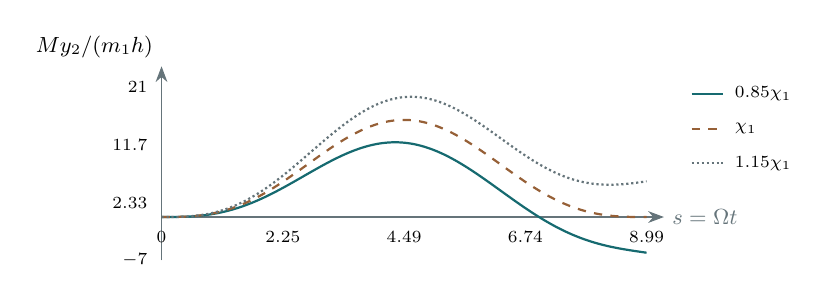
\begin{tikzpicture}[scale=.88,transform shape]
\draw[axis] (0,0.6250000)--(7.25,0.6250000) node[right] {$s=\Omega t$};
\draw[axis] (0.0000000,0)--(0.0000000,2.8);
\node[above left] at (0.0000000,2.8) {$My_2/(m_1h)$};
\node[below,font=\scriptsize] at (0.0000000,0.5450000) {$0$};
\node[below,font=\scriptsize] at (1.7500000,0.5450000) {$2.25$};
\node[below,font=\scriptsize] at (3.5000000,0.5450000) {$4.49$};
\node[below,font=\scriptsize] at (5.2500000,0.5450000) {$6.74$};
\node[below,font=\scriptsize] at (7.0000000,0.5450000) {$8.99$};
\node[left,font=\scriptsize] at (-0.0800000,0.0000000) {$-7$};
\node[left,font=\scriptsize] at (-0.0800000,0.8333333) {$2.33$};
\node[left,font=\scriptsize] at (-0.0800000,1.6666667) {$11.7$};
\node[left,font=\scriptsize] at (-0.0800000,2.5000000) {$21$};
\draw[thick,color=accent] plot coordinates {(0.0000000,0.6250000) (0.0291667,0.6250030) (0.0583333,0.6250237) (0.0875000,0.6250799) (0.1166667,0.6251889) (0.1458333,0.6253678) (0.1750000,0.6256335) (0.2041667,0.6260025) (0.2333333,0.6264911) (0.2625000,0.6271153) (0.2916667,0.6278904) (0.3208333,0.6288318) (0.3500000,0.6299540) (0.3791667,0.6312715) (0.4083333,0.6327981) (0.4375000,0.6345472) (0.4666667,0.6365316) (0.4958333,0.6387639) (0.5250000,0.6412558) (0.5541667,0.6440187) (0.5833333,0.6470635) (0.6125000,0.6504002) (0.6416667,0.6540385) (0.6708333,0.6579875) (0.7000000,0.6622555) (0.7291667,0.6668505) (0.7583333,0.6717794) (0.7875000,0.6770489) (0.8166667,0.6826648) (0.8458333,0.6886323) (0.8750000,0.6949559) (0.9041667,0.7016395) (0.9333333,0.7086863) (0.9625000,0.7160988) (0.9916667,0.7238788) (1.0208333,0.7320273) (1.0500000,0.7405449) (1.0791667,0.7494312) (1.1083333,0.7586853) (1.1375000,0.7683056) (1.1666667,0.7782896) (1.1958333,0.7886344) (1.2250000,0.7993362) (1.2541667,0.8103907) (1.2833333,0.8217928) (1.3125000,0.8335368) (1.3416667,0.8456164) (1.3708333,0.8580244) (1.4000000,0.8707533) (1.4291667,0.8837948) (1.4583333,0.8971399) (1.4875000,0.9107792) (1.5166667,0.9247026) (1.5458333,0.9388995) (1.5750000,0.9533585) (1.6041667,0.9680681) (1.6333333,0.9830158) (1.6625000,0.9981889) (1.6916667,1.0135741) (1.7208333,1.0291576) (1.7500000,1.0449253) (1.7791667,1.0608625) (1.8083333,1.0769540) (1.8375000,1.0931846) (1.8666667,1.1095383) (1.8958333,1.1259989) (1.9250000,1.1425501) (1.9541667,1.1591749) (1.9833333,1.1758564) (2.0125000,1.1925771) (2.0416667,1.2093195) (2.0708333,1.2260659) (2.1000000,1.2427982) (2.1291667,1.2594985) (2.1583333,1.2761484) (2.1875000,1.2927296) (2.2166667,1.3092237) (2.2458333,1.3256123) (2.2750000,1.3418767) (2.3041667,1.3579986) (2.3333333,1.3739594) (2.3625000,1.3897408) (2.3916667,1.4053243) (2.4208333,1.4206917) (2.4500000,1.4358249) (2.4791667,1.4507059) (2.5083333,1.4653169) (2.5375000,1.4796404) (2.5666667,1.4936590) (2.5958333,1.5073555) (2.6250000,1.5207132) (2.6541667,1.5337155) (2.6833333,1.5463462) (2.7125000,1.5585894) (2.7416667,1.5704296) (2.7708333,1.5818518) (2.8000000,1.5928412) (2.8291667,1.6033835) (2.8583333,1.6134650) (2.8875000,1.6230724) (2.9166667,1.6321926) (2.9458333,1.6408135) (2.9750000,1.6489231) (3.0041667,1.6565102) (3.0333333,1.6635642) (3.0625000,1.6700747) (3.0916667,1.6760323) (3.1208333,1.6814279) (3.1500000,1.6862533) (3.1791667,1.6905007) (3.2083333,1.6941630) (3.2375000,1.6972338) (3.2666667,1.6997072) (3.2958333,1.7015781) (3.3250000,1.7028421) (3.3541667,1.7034954) (3.3833333,1.7035348) (3.4125000,1.7029580) (3.4416667,1.7017631) (3.4708333,1.6999492) (3.5000000,1.6975159) (3.5291667,1.6944635) (3.5583333,1.6907931) (3.5875000,1.6865064) (3.6166667,1.6816058) (3.6458333,1.6760944) (3.6750000,1.6699760) (3.7041667,1.6632550) (3.7333333,1.6559366) (3.7625000,1.6480265) (3.7916667,1.6395312) (3.8208333,1.6304578) (3.8500000,1.6208139) (3.8791667,1.6106079) (3.9083333,1.5998489) (3.9375000,1.5885463) (3.9666667,1.5767102) (3.9958333,1.5643514) (4.0250000,1.5514812) (4.0541667,1.5381114) (4.0833333,1.5242543) (4.1125000,1.5099227) (4.1416667,1.4951301) (4.1708333,1.4798901) (4.2000000,1.4642171) (4.2291667,1.4481257) (4.2583333,1.4316311) (4.2875000,1.4147487) (4.3166667,1.3974944) (4.3458333,1.3798844) (4.3750000,1.3619353) (4.4041667,1.3436638) (4.4333333,1.3250870) (4.4625000,1.3062224) (4.4916667,1.2870874) (4.5208333,1.2677000) (4.5500000,1.2480780) (4.5791667,1.2282395) (4.6083333,1.2082029) (4.6375000,1.1879865) (4.6666667,1.1676086) (4.6958333,1.1470878) (4.7250000,1.1264426) (4.7541667,1.1056915) (4.7833333,1.0848529) (4.8125000,1.0639453) (4.8416667,1.0429870) (4.8708333,1.0219962) (4.9000000,1.0009911) (4.9291667,0.9799896) (4.9583333,0.9590095) (4.9875000,0.9380684) (5.0166667,0.9171835) (5.0458333,0.8963720) (5.0750000,0.8756506) (5.1041667,0.8550360) (5.1333333,0.8345441) (5.1625000,0.8141910) (5.1916667,0.7939920) (5.2208333,0.7739622) (5.2500000,0.7541162) (5.2791667,0.7344683) (5.3083333,0.7150323) (5.3375000,0.6958214) (5.3666667,0.6768485) (5.3958333,0.6581257) (5.4250000,0.6396650) (5.4541667,0.6214776) (5.4833333,0.6035740) (5.5125000,0.5859644) (5.5416667,0.5686584) (5.5708333,0.5516647) (5.6000000,0.5349918) (5.6291667,0.5186472) (5.6583333,0.5026380) (5.6875000,0.4869706) (5.7166667,0.4716507) (5.7458333,0.4566833) (5.7750000,0.4420730) (5.8041667,0.4278233) (5.8333333,0.4139374) (5.8625000,0.4004176) (5.8916667,0.3872656) (5.9208333,0.3744822) (5.9500000,0.3620679) (5.9791667,0.3500222) (6.0083333,0.3383441) (6.0375000,0.3270316) (6.0666667,0.3160823) (6.0958333,0.3054932) (6.1250000,0.2952602) (6.1541667,0.2853789) (6.1833333,0.2758442) (6.2125000,0.2666501) (6.2416667,0.2577901) (6.2708333,0.2492572) (6.3000000,0.2410435) (6.3291667,0.2331406) (6.3583333,0.2255394) (6.3875000,0.2182305) (6.4166667,0.2112036) (6.4458333,0.2044478) (6.4750000,0.1979520) (6.5041667,0.1917042) (6.5333333,0.1856920) (6.5625000,0.1799025) (6.5916667,0.1743224) (6.6208333,0.1689378) (6.6500000,0.1637343) (6.6791667,0.1586974) (6.7083333,0.1538117) (6.7375000,0.1490619) (6.7666667,0.1444319) (6.7958333,0.1399056) (6.8250000,0.1354664) (6.8541667,0.1310975) (6.8833333,0.1267816) (6.9125000,0.1225015) (6.9416667,0.1182396) (6.9708333,0.1139779) (7.0000000,0.1096986)};
\draw[thick,color=accent] (7.65,2.4)--(8.1,2.4);\node[right,font=\scriptsize] at (8.15,2.4) {$0.85\chi_1$};
\draw[thick,dashed,color=warm] plot coordinates {(0.0000000,0.6250000) (0.0291667,0.6250035) (0.0583333,0.6250280) (0.0875000,0.6250941) (0.1166667,0.6252226) (0.1458333,0.6254335) (0.1750000,0.6257469) (0.2041667,0.6261825) (0.2333333,0.6267596) (0.2625000,0.6274970) (0.2916667,0.6284133) (0.3208333,0.6295268) (0.3500000,0.6308549) (0.3791667,0.6324148) (0.4083333,0.6342234) (0.4375000,0.6362966) (0.4666667,0.6386502) (0.4958333,0.6412992) (0.5250000,0.6442580) (0.5541667,0.6475404) (0.5833333,0.6511597) (0.6125000,0.6551285) (0.6416667,0.6594585) (0.6708333,0.6641612) (0.7000000,0.6692469) (0.7291667,0.6747255) (0.7583333,0.6806061) (0.7875000,0.6868970) (0.8166667,0.6936057) (0.8458333,0.7007392) (0.8750000,0.7083035) (0.9041667,0.7163039) (0.9333333,0.7247448) (0.9625000,0.7336299) (0.9916667,0.7429622) (1.0208333,0.7527438) (1.0500000,0.7629759) (1.0791667,0.7736590) (1.1083333,0.7847929) (1.1375000,0.7963763) (1.1666667,0.8084074) (1.1958333,0.8208834) (1.2250000,0.8338008) (1.2541667,0.8471552) (1.2833333,0.8609415) (1.3125000,0.8751538) (1.3416667,0.8897855) (1.3708333,0.9048290) (1.4000000,0.9202763) (1.4291667,0.9361184) (1.4583333,0.9523456) (1.4875000,0.9689475) (1.5166667,0.9859131) (1.5458333,1.0032307) (1.5750000,1.0208876) (1.6041667,1.0388710) (1.6333333,1.0571671) (1.6625000,1.0757615) (1.6916667,1.0946393) (1.7208333,1.1137850) (1.7500000,1.1331826) (1.7791667,1.1528156) (1.8083333,1.1726667) (1.8375000,1.1927185) (1.8666667,1.2129529) (1.8958333,1.2333515) (1.9250000,1.2538955) (1.9541667,1.2745655) (1.9833333,1.2953421) (2.0125000,1.3162052) (2.0416667,1.3371347) (2.0708333,1.3581101) (2.1000000,1.3791107) (2.1291667,1.4001155) (2.1583333,1.4211035) (2.1875000,1.4420533) (2.2166667,1.4629436) (2.2458333,1.4837530) (2.2750000,1.5044598) (2.3041667,1.5250425) (2.3333333,1.5454796) (2.3625000,1.5657494) (2.3916667,1.5858305) (2.4208333,1.6057016) (2.4500000,1.6253413) (2.4791667,1.6447284) (2.5083333,1.6638422) (2.5375000,1.6826617) (2.5666667,1.7011665) (2.5958333,1.7193364) (2.6250000,1.7371515) (2.6541667,1.7545920) (2.6833333,1.7716387) (2.7125000,1.7882728) (2.7416667,1.8044757) (2.7708333,1.8202294) (2.8000000,1.8355162) (2.8291667,1.8503191) (2.8583333,1.8646213) (2.8875000,1.8784069) (2.9166667,1.8916602) (2.9458333,1.9043662) (2.9750000,1.9165106) (3.0041667,1.9280797) (3.0333333,1.9390601) (3.0625000,1.9494395) (3.0916667,1.9592060) (3.1208333,1.9683485) (3.1500000,1.9768565) (3.1791667,1.9847202) (3.2083333,1.9919308) (3.2375000,1.9984798) (3.2666667,2.0043599) (3.2958333,2.0095642) (3.3250000,2.0140868) (3.3541667,2.0179224) (3.3833333,2.0210667) (3.4125000,2.0235160) (3.4416667,2.0252675) (3.4708333,2.0263192) (3.5000000,2.0266699) (3.5291667,2.0263192) (3.5583333,2.0252675) (3.5875000,2.0235160) (3.6166667,2.0210667) (3.6458333,2.0179224) (3.6750000,2.0140868) (3.7041667,2.0095642) (3.7333333,2.0043599) (3.7625000,1.9984798) (3.7916667,1.9919308) (3.8208333,1.9847202) (3.8500000,1.9768565) (3.8791667,1.9683485) (3.9083333,1.9592060) (3.9375000,1.9494395) (3.9666667,1.9390601) (3.9958333,1.9280797) (4.0250000,1.9165106) (4.0541667,1.9043662) (4.0833333,1.8916602) (4.1125000,1.8784069) (4.1416667,1.8646213) (4.1708333,1.8503191) (4.2000000,1.8355162) (4.2291667,1.8202294) (4.2583333,1.8044757) (4.2875000,1.7882728) (4.3166667,1.7716387) (4.3458333,1.7545920) (4.3750000,1.7371515) (4.4041667,1.7193364) (4.4333333,1.7011665) (4.4625000,1.6826617) (4.4916667,1.6638422) (4.5208333,1.6447284) (4.5500000,1.6253413) (4.5791667,1.6057016) (4.6083333,1.5858305) (4.6375000,1.5657494) (4.6666667,1.5454796) (4.6958333,1.5250425) (4.7250000,1.5044598) (4.7541667,1.4837530) (4.7833333,1.4629436) (4.8125000,1.4420533) (4.8416667,1.4211035) (4.8708333,1.4001155) (4.9000000,1.3791107) (4.9291667,1.3581101) (4.9583333,1.3371347) (4.9875000,1.3162052) (5.0166667,1.2953421) (5.0458333,1.2745655) (5.0750000,1.2538955) (5.1041667,1.2333515) (5.1333333,1.2129529) (5.1625000,1.1927185) (5.1916667,1.1726667) (5.2208333,1.1528156) (5.2500000,1.1331826) (5.2791667,1.1137850) (5.3083333,1.0946393) (5.3375000,1.0757615) (5.3666667,1.0571671) (5.3958333,1.0388710) (5.4250000,1.0208876) (5.4541667,1.0032307) (5.4833333,0.9859131) (5.5125000,0.9689475) (5.5416667,0.9523456) (5.5708333,0.9361184) (5.6000000,0.9202763) (5.6291667,0.9048290) (5.6583333,0.8897855) (5.6875000,0.8751538) (5.7166667,0.8609415) (5.7458333,0.8471552) (5.7750000,0.8338008) (5.8041667,0.8208834) (5.8333333,0.8084074) (5.8625000,0.7963763) (5.8916667,0.7847929) (5.9208333,0.7736590) (5.9500000,0.7629759) (5.9791667,0.7527438) (6.0083333,0.7429622) (6.0375000,0.7336299) (6.0666667,0.7247448) (6.0958333,0.7163039) (6.1250000,0.7083035) (6.1541667,0.7007392) (6.1833333,0.6936057) (6.2125000,0.6868970) (6.2416667,0.6806061) (6.2708333,0.6747255) (6.3000000,0.6692469) (6.3291667,0.6641612) (6.3583333,0.6594585) (6.3875000,0.6551285) (6.4166667,0.6511597) (6.4458333,0.6475404) (6.4750000,0.6442580) (6.5041667,0.6412992) (6.5333333,0.6386502) (6.5625000,0.6362966) (6.5916667,0.6342234) (6.6208333,0.6324148) (6.6500000,0.6308549) (6.6791667,0.6295268) (6.7083333,0.6284133) (6.7375000,0.6274970) (6.7666667,0.6267596) (6.7958333,0.6261825) (6.8250000,0.6257469) (6.8541667,0.6254335) (6.8833333,0.6252226) (6.9125000,0.6250941) (6.9416667,0.6250280) (6.9708333,0.6250035) (7.0000000,0.6250000)};
\draw[thick,dashed,color=warm] (7.65,1.9)--(8.1,1.9);\node[right,font=\scriptsize] at (8.15,1.9) {$\chi_1$};
\draw[thick,densely dotted,color=muted] plot coordinates {(0.0000000,0.6250000) (0.0291667,0.6250040) (0.0583333,0.6250322) (0.0875000,0.6251083) (0.1166667,0.6252562) (0.1458333,0.6254992) (0.1750000,0.6258604) (0.2041667,0.6263625) (0.2333333,0.6270280) (0.2625000,0.6278787) (0.2916667,0.6289363) (0.3208333,0.6302217) (0.3500000,0.6317557) (0.3791667,0.6335582) (0.4083333,0.6356487) (0.4375000,0.6380461) (0.4666667,0.6407688) (0.4958333,0.6438345) (0.5250000,0.6472601) (0.5541667,0.6510620) (0.5833333,0.6552559) (0.6125000,0.6598567) (0.6416667,0.6648786) (0.6708333,0.6703349) (0.7000000,0.6762383) (0.7291667,0.6826006) (0.7583333,0.6894328) (0.7875000,0.6967450) (0.8166667,0.7045467) (0.8458333,0.7128462) (0.8750000,0.7216511) (0.9041667,0.7309682) (0.9333333,0.7408032) (0.9625000,0.7511610) (0.9916667,0.7620457) (1.0208333,0.7734602) (1.0500000,0.7854069) (1.0791667,0.7978869) (1.1083333,0.8109005) (1.1375000,0.8244471) (1.1666667,0.8385252) (1.1958333,0.8531324) (1.2250000,0.8682653) (1.2541667,0.8839196) (1.2833333,0.9000901) (1.3125000,0.9167707) (1.3416667,0.9339546) (1.3708333,0.9516337) (1.4000000,0.9697994) (1.4291667,0.9884420) (1.4583333,1.0075513) (1.4875000,1.0271159) (1.5166667,1.0471237) (1.5458333,1.0675618) (1.5750000,1.0884167) (1.6041667,1.1096740) (1.6333333,1.1313183) (1.6625000,1.1533340) (1.6916667,1.1757045) (1.7208333,1.1984124) (1.7500000,1.2214400) (1.7791667,1.2447687) (1.8083333,1.2683794) (1.8375000,1.2922524) (1.8666667,1.3163676) (1.8958333,1.3407042) (1.9250000,1.3652409) (1.9541667,1.3899561) (1.9833333,1.4148278) (2.0125000,1.4398333) (2.0416667,1.4649499) (2.0708333,1.4901543) (2.1000000,1.5154231) (2.1291667,1.5407325) (2.1583333,1.5660585) (2.1875000,1.5913770) (2.2166667,1.6166635) (2.2458333,1.6418937) (2.2750000,1.6670429) (2.3041667,1.6920864) (2.3333333,1.7169997) (2.3625000,1.7417580) (2.3916667,1.7663368) (2.4208333,1.7907115) (2.4500000,1.8148577) (2.4791667,1.8387510) (2.5083333,1.8623674) (2.5375000,1.8856830) (2.5666667,1.9086741) (2.5958333,1.9313173) (2.6250000,1.9535897) (2.6541667,1.9754685) (2.6833333,1.9969313) (2.7125000,2.0179562) (2.7416667,2.0385218) (2.7708333,2.0586070) (2.8000000,2.0781912) (2.8291667,2.0972546) (2.8583333,2.1157776) (2.8875000,2.1337414) (2.9166667,2.1511277) (2.9458333,2.1679190) (2.9750000,2.1840982) (3.0041667,2.1996491) (3.0333333,2.2145561) (3.0625000,2.2288043) (3.0916667,2.2423798) (3.1208333,2.2552690) (3.1500000,2.2674596) (3.1791667,2.2789398) (3.2083333,2.2896986) (3.2375000,2.2997259) (3.2666667,2.3090126) (3.2958333,2.3175503) (3.3250000,2.3253314) (3.3541667,2.3323494) (3.3833333,2.3385985) (3.4125000,2.3440740) (3.4416667,2.3487719) (3.4708333,2.3526892) (3.5000000,2.3558239) (3.5291667,2.3581749) (3.5583333,2.3597418) (3.5875000,2.3605255) (3.6166667,2.3605275) (3.6458333,2.3597503) (3.6750000,2.3581975) (3.7041667,2.3558734) (3.7333333,2.3527832) (3.7625000,2.3489332) (3.7916667,2.3443304) (3.8208333,2.3389827) (3.8500000,2.3328991) (3.8791667,2.3260890) (3.9083333,2.3185631) (3.9375000,2.3103328) (3.9666667,2.3014100) (3.9958333,2.2918079) (4.0250000,2.2815401) (4.0541667,2.2706210) (4.0833333,2.2590661) (4.1125000,2.2468910) (4.1416667,2.2341126) (4.1708333,2.2207480) (4.2000000,2.2068153) (4.2291667,2.1923330) (4.2583333,2.1773203) (4.2875000,2.1617969) (4.3166667,2.1457830) (4.3458333,2.1292995) (4.3750000,2.1123676) (4.4041667,2.0950091) (4.4333333,2.0772460) (4.4625000,2.0591010) (4.4916667,2.0405969) (4.5208333,2.0217569) (4.5500000,2.0026045) (4.5791667,1.9831636) (4.6083333,1.9634582) (4.6375000,1.9435123) (4.6666667,1.9233505) (4.6958333,1.9029972) (4.7250000,1.8824770) (4.7541667,1.8618144) (4.7833333,1.8410343) (4.8125000,1.8201613) (4.8416667,1.7992199) (4.8708333,1.7782347) (4.9000000,1.7572302) (4.9291667,1.7362305) (4.9583333,1.7152598) (4.9875000,1.6943420) (5.0166667,1.6735006) (5.0458333,1.6527591) (5.0750000,1.6321403) (5.1041667,1.6116671) (5.1333333,1.5913617) (5.1625000,1.5712460) (5.1916667,1.5513414) (5.2208333,1.5316690) (5.2500000,1.5122491) (5.2791667,1.4931017) (5.3083333,1.4742463) (5.3375000,1.4557015) (5.3666667,1.4374857) (5.3958333,1.4196163) (5.4250000,1.4021102) (5.4541667,1.3849837) (5.4833333,1.3682523) (5.5125000,1.3519306) (5.5416667,1.3360328) (5.5708333,1.3205721) (5.6000000,1.3055609) (5.6291667,1.2910109) (5.6583333,1.2769329) (5.6875000,1.2633370) (5.7166667,1.2502323) (5.7458333,1.2376270) (5.7750000,1.2255285) (5.8041667,1.2139435) (5.8333333,1.2028774) (5.8625000,1.1923351) (5.8916667,1.1823202) (5.9208333,1.1728359) (5.9500000,1.1638839) (5.9791667,1.1554653) (6.0083333,1.1475804) (6.0375000,1.1402282) (6.0666667,1.1334072) (6.0958333,1.1271146) (6.1250000,1.1213468) (6.1541667,1.1160995) (6.1833333,1.1113673) (6.2125000,1.1071438) (6.2416667,1.1034220) (6.2708333,1.1001938) (6.3000000,1.0974504) (6.3291667,1.0951818) (6.3583333,1.0933776) (6.3875000,1.0920264) (6.4166667,1.0911158) (6.4458333,1.0906329) (6.4750000,1.0905639) (6.5041667,1.0908942) (6.5333333,1.0916085) (6.5625000,1.0926908) (6.5916667,1.0941244) (6.6208333,1.0958919) (6.6500000,1.0979754) (6.6791667,1.1003561) (6.7083333,1.1030150) (6.7375000,1.1059321) (6.7666667,1.1090872) (6.7958333,1.1124594) (6.8250000,1.1160274) (6.8541667,1.1197695) (6.8833333,1.1236635) (6.9125000,1.1276867) (6.9416667,1.1318164) (6.9708333,1.1360291) (7.0000000,1.1403014)};
\draw[thick,densely dotted,color=muted] (7.65,1.4)--(8.1,1.4);\node[right,font=\scriptsize] at (8.15,1.4) {$1.15\chi_1$};
\end{tikzpicture}
\figcaption{变图综二.2V7\quad 改变离地速度会移动壳底再次到达地面的时刻}
\end{minipage}\end{center}
\item \textbf{用壳半径反求最低刚度。}取等质量$m$，要求球在首根飞行及初始压低时均处于壳内。图V8的波峰与波谷给$A_d/h=\sqrt{1+\chi_1^2}$。初始位置离中心向下的距离是$h+H_{\min}$，故
\[
\kappa>\sqrt{1+\chi_1^2},\qquad
\kappa>1+\sqrt{4+2\chi_1^2}.
\]
后者较强，约为$\kappa>7.662$。这个限制来自初始下拉位置，飞行中的相对运动还有余量。
\begin{center}\begin{minipage}{.98\linewidth}\centering
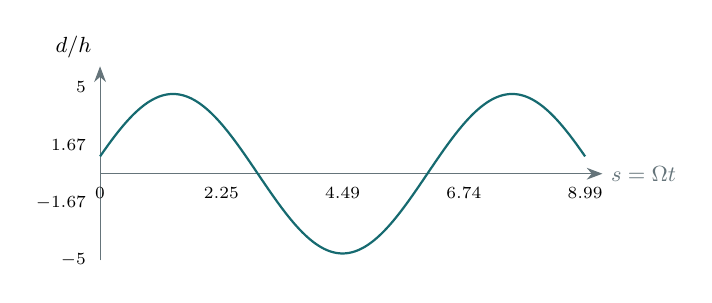
\begin{tikzpicture}[scale=.88,transform shape]
\draw[axis] (0,1.2500000)--(7.25,1.2500000) node[right] {$s=\Omega t$};
\draw[axis] (0.0000000,0)--(0.0000000,2.8);
\node[above left] at (0.0000000,2.8) {$d/h$};
\node[below,font=\scriptsize] at (0.0000000,1.1700000) {$0$};
\node[below,font=\scriptsize] at (1.7500000,1.1700000) {$2.25$};
\node[below,font=\scriptsize] at (3.5000000,1.1700000) {$4.49$};
\node[below,font=\scriptsize] at (5.2500000,1.1700000) {$6.74$};
\node[below,font=\scriptsize] at (7.0000000,1.1700000) {$8.99$};
\node[left,font=\scriptsize] at (-0.0800000,0.0000000) {$-5$};
\node[left,font=\scriptsize] at (-0.0800000,0.8333333) {$-1.67$};
\node[left,font=\scriptsize] at (-0.0800000,1.6666667) {$1.67$};
\node[left,font=\scriptsize] at (-0.0800000,2.5000000) {$5$};
\draw[thick,color=accent] plot coordinates {(0.0000000,1.5000000) (0.0291667,1.5418789) (0.0583333,1.5833487) (0.0875000,1.6243511) (0.1166667,1.6648286) (0.1458333,1.7047246) (0.1750000,1.7439831) (0.2041667,1.7825490) (0.2333333,1.8203683) (0.2625000,1.8573880) (0.2916667,1.8935561) (0.3208333,1.9288220) (0.3500000,1.9631362) (0.3791667,1.9964506) (0.4083333,2.0287185) (0.4375000,2.0598947) (0.4666667,2.0899354) (0.4958333,2.1187985) (0.5250000,2.1464436) (0.5541667,2.1728320) (0.5833333,2.1979265) (0.6125000,2.2216921) (0.6416667,2.2440954) (0.6708333,2.2651050) (0.7000000,2.2846914) (0.7291667,2.3028273) (0.7583333,2.3194871) (0.7875000,2.3346475) (0.8166667,2.3482873) (0.8458333,2.3603873) (0.8750000,2.3709306) (0.9041667,2.3799024) (0.9333333,2.3872901) (0.9625000,2.3930834) (0.9916667,2.3972740) (1.0208333,2.3998563) (1.0500000,2.4008264) (1.0791667,2.4001832) (1.1083333,2.3979274) (1.1375000,2.3940623) (1.1666667,2.3885932) (1.1958333,2.3815278) (1.2250000,2.3728761) (1.2541667,2.3626501) (1.2833333,2.3508643) (1.3125000,2.3375350) (1.3416667,2.3226811) (1.3708333,2.3063233) (1.4000000,2.2884846) (1.4291667,2.2691899) (1.4583333,2.2484664) (1.4875000,2.2263430) (1.5166667,2.2028509) (1.5458333,2.1780228) (1.5750000,2.1518938) (1.6041667,2.1245002) (1.6333333,2.0958807) (1.6625000,2.0660753) (1.6916667,2.0351257) (1.7208333,2.0030755) (1.7500000,1.9699694) (1.7791667,1.9358540) (1.8083333,1.9007770) (1.8375000,1.8647876) (1.8666667,1.8279364) (1.8958333,1.7902748) (1.9250000,1.7518559) (1.9541667,1.7127333) (1.9833333,1.6729620) (2.0125000,1.6325978) (2.0416667,1.5916971) (2.0708333,1.5503174) (2.1000000,1.5085166) (2.1291667,1.4663535) (2.1583333,1.4238870) (2.1875000,1.3811767) (2.2166667,1.3382825) (2.2458333,1.2952645) (2.2750000,1.2521831) (2.3041667,1.2090986) (2.3333333,1.1660715) (2.3625000,1.1231620) (2.3916667,1.0804304) (2.4208333,1.0379365) (2.4500000,0.9957398) (2.4791667,0.9538997) (2.5083333,0.9124747) (2.5375000,0.8715229) (2.5666667,0.8311017) (2.5958333,0.7912677) (2.6250000,0.7520769) (2.6541667,0.7135842) (2.6833333,0.6758435) (2.7125000,0.6389078) (2.7416667,0.6028288) (2.7708333,0.5676571) (2.8000000,0.5334420) (2.8291667,0.5002316) (2.8583333,0.4680723) (2.8875000,0.4370092) (2.9166667,0.4070859) (2.9458333,0.3783443) (2.9750000,0.3508248) (3.0041667,0.3245659) (3.0333333,0.2996045) (3.0625000,0.2759754) (3.0916667,0.2537120) (3.1208333,0.2328452) (3.1500000,0.2134045) (3.1791667,0.1954171) (3.2083333,0.1789082) (3.2375000,0.1639009) (3.2666667,0.1504163) (3.2958333,0.1384733) (3.3250000,0.1280886) (3.3541667,0.1192767) (3.3833333,0.1120502) (3.4125000,0.1064190) (3.4416667,0.1023910) (3.4708333,0.0999720) (3.5000000,0.0991653) (3.5291667,0.0999720) (3.5583333,0.1023910) (3.5875000,0.1064190) (3.6166667,0.1120502) (3.6458333,0.1192767) (3.6750000,0.1280886) (3.7041667,0.1384733) (3.7333333,0.1504163) (3.7625000,0.1639009) (3.7916667,0.1789082) (3.8208333,0.1954171) (3.8500000,0.2134045) (3.8791667,0.2328452) (3.9083333,0.2537120) (3.9375000,0.2759754) (3.9666667,0.2996045) (3.9958333,0.3245659) (4.0250000,0.3508248) (4.0541667,0.3783443) (4.0833333,0.4070859) (4.1125000,0.4370092) (4.1416667,0.4680723) (4.1708333,0.5002316) (4.2000000,0.5334420) (4.2291667,0.5676571) (4.2583333,0.6028288) (4.2875000,0.6389078) (4.3166667,0.6758435) (4.3458333,0.7135842) (4.3750000,0.7520769) (4.4041667,0.7912677) (4.4333333,0.8311017) (4.4625000,0.8715229) (4.4916667,0.9124747) (4.5208333,0.9538997) (4.5500000,0.9957398) (4.5791667,1.0379365) (4.6083333,1.0804304) (4.6375000,1.1231620) (4.6666667,1.1660715) (4.6958333,1.2090986) (4.7250000,1.2521831) (4.7541667,1.2952645) (4.7833333,1.3382825) (4.8125000,1.3811767) (4.8416667,1.4238870) (4.8708333,1.4663535) (4.9000000,1.5085166) (4.9291667,1.5503174) (4.9583333,1.5916971) (4.9875000,1.6325978) (5.0166667,1.6729620) (5.0458333,1.7127333) (5.0750000,1.7518559) (5.1041667,1.7902748) (5.1333333,1.8279364) (5.1625000,1.8647876) (5.1916667,1.9007770) (5.2208333,1.9358540) (5.2500000,1.9699694) (5.2791667,2.0030755) (5.3083333,2.0351257) (5.3375000,2.0660753) (5.3666667,2.0958807) (5.3958333,2.1245002) (5.4250000,2.1518938) (5.4541667,2.1780228) (5.4833333,2.2028509) (5.5125000,2.2263430) (5.5416667,2.2484664) (5.5708333,2.2691899) (5.6000000,2.2884846) (5.6291667,2.3063233) (5.6583333,2.3226811) (5.6875000,2.3375350) (5.7166667,2.3508643) (5.7458333,2.3626501) (5.7750000,2.3728761) (5.8041667,2.3815278) (5.8333333,2.3885932) (5.8625000,2.3940623) (5.8916667,2.3979274) (5.9208333,2.4001832) (5.9500000,2.4008264) (5.9791667,2.3998563) (6.0083333,2.3972740) (6.0375000,2.3930834) (6.0666667,2.3872901) (6.0958333,2.3799024) (6.1250000,2.3709306) (6.1541667,2.3603873) (6.1833333,2.3482873) (6.2125000,2.3346475) (6.2416667,2.3194871) (6.2708333,2.3028273) (6.3000000,2.2846914) (6.3291667,2.2651050) (6.3583333,2.2440954) (6.3875000,2.2216921) (6.4166667,2.1979265) (6.4458333,2.1728320) (6.4750000,2.1464436) (6.5041667,2.1187985) (6.5333333,2.0899354) (6.5625000,2.0598947) (6.5916667,2.0287185) (6.6208333,1.9964506) (6.6500000,1.9631362) (6.6791667,1.9288220) (6.7083333,1.8935561) (6.7375000,1.8573880) (6.7666667,1.8203683) (6.7958333,1.7825490) (6.8250000,1.7439831) (6.8541667,1.7047246) (6.8833333,1.6648286) (6.9125000,1.6243511) (6.9416667,1.5833487) (6.9708333,1.5418789) (7.0000000,1.5000000)};
\end{tikzpicture}
\figcaption{变图综二.2V8\quad 相对位置达到的两端极值给出壳内空间要求}
\end{minipage}\end{center}
\end{enumerate}

\Needspace{13\baselineskip}

\pdfbookmark[2]{第 3 题 以连续折射求最速降线}{q3}

\section*{第 3 题\quad 以连续折射求最速降线}\label{q:3}


在均匀重力场中取水平向右$x$轴、竖直向下$y$轴，起点$O=(0,0)$，终点$P=(a,b)$，$a,b>0$。质点从$O$静止出发，沿位于竖直平面的光滑轨道无摩擦滑至$P$。

参照连续水平分层介质中的折射规律，求所需时间最短的轨道。给出轨道参数方程、由$a,b$确定参数的条件和最短时间；说明终点可能在轨道最低点之后，以及怎样确认所得曲线确为时间最小。


\begin{center}\begin{minipage}{.98\linewidth}\centering
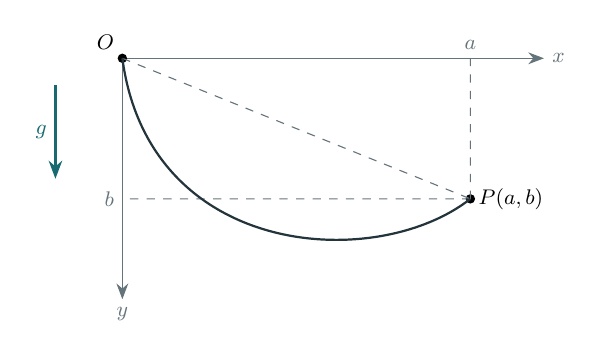
\begin{tikzpicture}[scale=.85,transform shape]

\draw[axis] (0,0)--(6.3,0) node[right] {$x$};
\draw[axis] (0,0)--(0,-3.6) node[below] {$y$};
\fill (0,0) circle (2pt) node[above left] {$O$};
\coordinate (P) at (5.2,-2.1);
\fill (P) circle (2pt) node[right] {$P(a,b)$};
\draw[guide] (P)--(5.2,0) node[above] {$a$};
\draw[guide] (P)--(0,-2.1) node[left] {$b$};
\draw[guide] (0,0)--(P);
\draw[object] (0,0) .. controls (.4,-3) and (3.8,-3.2) .. (P);
\draw[motion] (-1,-.4)--(-1,-1.8) node[midway,left] {$g$};

\end{tikzpicture}
\figcaption{图综二.3\quad 两端点和候选光滑轨道；坐标y沿重力方向向下。}
\end{minipage}\end{center}

\Needspace{8\baselineskip}

\pdfbookmark[3]{题型定位}{q3-h0}

\subsection*{题型定位}

把分层光路的时间驻值条件移到均匀重力场中的滑动问题。给定端点先决定摆线的尺度和末相位，末相位决定轨道是否经过最低点。用同起点摆线族构造时间函数，证明这条驻值轨道达到全体可行路径的时间下界。

\Needspace{8\baselineskip}

\pdfbookmark[3]{知识点}{q3-h1}

\subsection*{知识点}

\begin{itemize}
\item 能量守恒的高度速率、连续分层折射。
\item 切线角与入射角的互余关系、时间泛函第一积分。
\item 摆线参数、末点比例的单调性与有限起步时间。
\item 驻值与最小值的区别、时间函数梯度和路径积分下界。
\end{itemize}

\Needspace{8\baselineskip}

\pdfbookmark[3]{物理图像}{q3-h2}

\subsection*{物理图像}

解图综二.3A在水平分层处标两种角，B把最低点及其后的上升段一起画出，C画同起点摆线族及到达时间的梯度方向。三图分别用于折射条件、端点分支和最短时间证明。

\Needspace{8\baselineskip}

\pdfbookmark[3]{解题入口}{q3-h3}

\subsection*{解题入口}

从图A的界面交点移动入手。路长改变量分别乘对应层的倒速率，得到两侧相同的$\sin\theta/v$。将$\theta$换成与水平的夹角$\alpha$，再以$v=\sqrt{2gy}$化成斜率方程。图B的$\varphi$贯穿最低点，$\cot(\varphi/2)$的符号随之改变。由终点比例求参数和时间，最后在图C对任意小位移作切向投影，得到$d\mathcal T\le dt$。

\Needspace{8\baselineskip}

\pdfbookmark[3]{标准解法}{q3-h4}

\subsection*{标准解法}


图综二.3的$y$向下为正。能量守恒使任一高度处的速率只由$y$决定：
\[
v(y)=\sqrt{2gy}.
\]
较深处速度较大。终点离起点较远时，轨道先下降取得较大速度，再上升至指定终点。

把图A中的水平线看作薄层的交界面。相邻两层的折射率为$n_1,n_2$，光速为$c/n_1,c/n_2$，折射定律$n_1\sin\theta_1=n_2\sin\theta_2$便给出$\sin\theta/v$在界面两侧相同。也可直接把界面交点向右移$\delta x$。在交点左边，路长的一阶增量是$\sin\theta_1\,\delta x$，右边则减少$\sin\theta_2\,\delta x$。传播时间的一阶增量为$(\sin\theta_1/v_1-\sin\theta_2/v_2)\delta x$，驻值处括号为零。让各层变薄并取粒子的$v(y)$，得到
\[
\frac{\sin\theta}{v(y)}=\text{常量}.
\]
其中$\theta$是切线与竖直法线夹角。若切线与水平轴夹角为$\alpha$，则$\sin\theta=\cos\alpha$，连续极限下
\[
\frac{\cos\alpha}{\sqrt{2gy}}=\text{常量}.
\]
\begin{center}\begin{minipage}{.98\linewidth}\centering
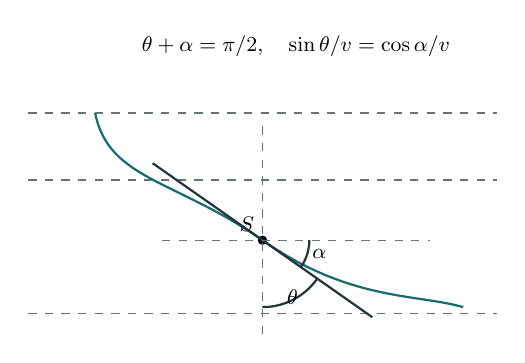
\begin{tikzpicture}[scale=.85,transform shape]

\foreach \y in {0,-1,-3}{\draw[guide] (-1,\y)--(6,\y);}
\draw[traj] (0,0) .. controls (.2,-1) and (1.2,-.99) .. (2.5,-1.9)
.. controls (3.8,-2.81) and (4.8,-2.7) .. (5.5,-2.9);
\coordinate (S) at (2.5,-1.9); \fill (S) circle (2pt) node[above left] {$S$};
\draw[object] (.86,-.75)--(4.14,-3.05);
\draw[guide] (2.5,-.2)--(2.5,-3.3);
\draw[guide] (1,-1.9)--(5,-1.9);
\draw[object] (3.2,-1.9) arc[start angle=0,end angle=-35,radius=.7];
\draw[object] (2.5,-2.9) arc[start angle=-90,end angle=-35,radius=1];
\node at (3.35,-2.1) {$\alpha$};
\node at (2.95,-2.75) {$\theta$};
\node at (3,1) {$\theta+\alpha=\pi/2,\quad \sin\theta/v=\cos\alpha/v$};

\end{tikzpicture}
\figcaption{解图综二.3A\quad 水平层的法线竖直，折射角与切线倾角互余。}
\end{minipage}\end{center}
解图综二.3A把入射角与切线倾角标在同一点。沿$x$增加的曲线有$\cos\alpha=1/\sqrt{1+y'^2}$，因而
\[
\boxed{y(1+y'^2)=A},\qquad A>0.
\]
时间泛函的被积式是$L=\sqrt{1+y'^2}/\sqrt{2gy}$，其中$y'=dy/dx$。$L$不显含$x$，沿驻值轨道的$L-y' L_{y'}$为常量。代入得$1/[\sqrt{2gy}\sqrt{1+y'^2}]$，正是图A由切线方向得到的同一常量。

为同时保留下降和上升的分支，令
\[
y=\frac A2(1-\cos\varphi),\qquad 0<\varphi<2\pi.
\]
此时
\[
y'^2=\frac Ay-1=\cot^2\frac\varphi2.
\]
沿一个无回绕摆线拱取$y'=\cot(\varphi/2)$，它在$\varphi=\pi$前为正、之后为负，与图B中下降段和上升段的方向相合。结合
$dy/d\varphi=(A/2)\sin\varphi$，得到
\[
\frac{dx}{d\varphi}
=\frac{(A/2)\sin\varphi}{\cot(\varphi/2)}
=\frac A2(1-\cos\varphi).
\]
在$\varphi=\pi$处，前式的商按化简后的连续值$A$取值。设$\beta=\varphi/2$，上式也就是$dx=2A\sin^2\beta\,d\beta$。起点对应$\beta=0$，积分为$x=\int_0^\beta A(1-\cos2u)\,du=A\beta-(A/2)\sin2\beta$。记$\mathcal R=A/2$，
\[
\boxed{x=\mathcal R(\varphi-\sin\varphi),\qquad
y=\mathcal R(1-\cos\varphi)}.
\]
它是摆线的第一个拱，起点处切线竖直，虽然初速为零，起步所需时间仍有限。
\begin{center}\begin{minipage}{.98\linewidth}\centering
\begin{tikzpicture}[scale=.85,transform shape]

\draw[axis] (0,0)--(6.8,0) node[right] {$x$};
\draw[axis] (0,0)--(0,-3) node[below] {$y$};
\draw[traj,domain=0:250,samples=220] plot ({.9*(rad(\x)-sin(\x))},{-.9*(1-cos(\x))});
\draw[guide,domain=250:330,samples=80] plot ({.9*(rad(\x)-sin(\x))},{-.9*(1-cos(\x))});
\fill (0,0) circle (2pt) node[above left] {$O$};
\fill (2.827433,-1.8) circle (2pt) node[below] {最低点$\varphi=\pi$};
\fill ({.9*(rad(250)-sin(250))},{-.9*(1-cos(250))}) circle (2pt) node[above right] {$P$示例};
\draw[motion] (0.968517,-1.266063)--(1.555586,-1.647310);
\draw[motion] (4.116674,-1.558218)--(4.767967,-1.301667);
\node at (3.3,1) {$x=\mathcal R(\varphi-\sin\varphi),\quad y=\mathcal R(1-\cos\varphi)$};
\node at (3.3,-4) {$a/b>\pi/2$时先降后升，末点在最低点之后};

\end{tikzpicture}
\figcaption{解图综二.3B\quad 单拱摆线在最低点前下降，过最低点后上升。}
\end{minipage}\end{center}
解图综二.3B标出$\varphi=\pi$的最低点和$\varphi>\pi$的上升段。终点条件为
\[
a=\mathcal R(\varphi_P-\sin\varphi_P),\qquad
b=\mathcal R(1-\cos\varphi_P).
\]
因此先解
\[
\boxed{\frac ab=
\frac{\varphi_P-\sin\varphi_P}{1-\cos\varphi_P}},
\quad 0<\varphi_P<2\pi,
\qquad
\boxed{\mathcal R=\frac b{1-\cos\varphi_P}}.
\]
这个比值从零严格增到无穷，故对任意$a,b>0$有唯一单拱解。例如求导分子可化为
$2(1-\cos\varphi)-\varphi\sin\varphi$；在$(0,\pi)$令$z=\varphi/2$，它为
$4\sin z(\sin z-z\cos z)>0$，在$(\pi,2\pi)$则两项都非负。
特别地
\[
\varphi_P\begin{cases}
<\pi,&a/b<\pi/2,\\
=\pi,&a/b=\pi/2,\\
>\pi,&a/b>\pi/2.
\end{cases}
\]
所以终点在最低点之前还是之后，应由横纵距离之比决定。

摆线弧长元与速率分别为
\[
ds=2\mathcal R\sin\frac\varphi2\,d\varphi,\qquad
v=2\sqrt{g\mathcal R}\sin\frac\varphi2,
\]
在$0<\varphi<2\pi$内正弦为正，因此
\[
dt=\sqrt{\frac{\mathcal R}{g}}\,d\varphi,
\qquad
\boxed{T_{\min}=\varphi_P\sqrt{\frac{\mathcal R}{g}}}.
\]
两个同时趋零的因子在起点相消，积分没有发散。
\begin{center}\begin{minipage}{.98\linewidth}\centering
\begin{tikzpicture}[scale=.85,transform shape]

\draw[axis] (0,0)--(8,0) node[right] {$x$};
\draw[axis] (0,0)--(0,-3.5) node[below] {$y$};
\foreach \a in {.45,.7,1,1.4}{
\draw[traj,domain=0:230,samples=170] plot ({\a*(rad(\x)-sin(\x))},{-\a*(1-cos(\x))});
}
\draw[force] (.7605,-1.17365)--(1.5265,-1.81665);
\node[right,text=warm] at (5.3,-.5) {$\nabla\mathcal T$沿切线};
\node at (4.7,1) {$|\nabla\mathcal T|=1/\sqrt{2gy}$};
\node at (4,-4.3) {沿摆线切向取等，任意其他路径满足$d\mathcal T\leq dt$};

\end{tikzpicture}
\figcaption{解图综二.3C\quad 同起点摆线族定义到达时间函数，梯度给最短时间的下界证明。}
\end{minipage}\end{center}
满足折射条件说明轨道使时间取驻值，还需比较任意其他路径。为确认它是最小值，解图综二.3C取由这些单拱摆线构成的轨道族。对任一点$(x,y)$、$x,y>0$，用唯一的$\mathcal R,\varphi$定义到达时间函数
\[
\mathcal T(x,y)=\varphi\sqrt{\frac{\mathcal R}{g}}.
\]
对两个参数分别微分，得到
\[
\mathcal T_x=\frac1{2\sqrt{g\mathcal R}},\qquad
\mathcal T_y=\frac{\cot(\varphi/2)}{2\sqrt{g\mathcal R}},
\qquad
|\nabla\mathcal T|=\frac1{\sqrt{2gy}}.
\]
具体地，将前两项乘$dx,dy$相加，$d\mathcal R$系数是
$[\varphi-\sin\varphi+\cot(\varphi/2)(1-\cos\varphi)]/(2\sqrt{g\mathcal R})
=\varphi/(2\sqrt{g\mathcal R})$，
$d\varphi$系数是$\sqrt{\mathcal R/g}$，恰为$d\mathcal T$。

沿任意可行轨道，柯西不等式给
\[
d\mathcal T=\nabla\mathcal T\cdot d\boldsymbol r
\leq |\nabla\mathcal T|\,ds
=\frac{ds}{\sqrt{2gy}}=dt.
\]
从起点积分，$\mathcal T(O)=0$，故
\[
T_{\rm path}\geq\mathcal T(P)
=\varphi_P\sqrt{\mathcal R/g}.
\]
摆线切向与$\nabla\mathcal T$同向，处处取等，因而达到这个下界。对$x<0$取偶延拓$\mathcal T(|x|,y)$。在$x$趋于零且$y>0$固定时，$\varphi\to0$，$\mathcal R(1-\cos\varphi)=y$给出$\mathcal T\to\sqrt{2y/g}$，同时$\mathcal T_x\to0$、$\mathcal T_y\to1/\sqrt{2gy}$。两侧的梯度在竖直轴上接合，因此同一不等式适用于整个$y>0$区域。

由能量守恒，可达区域为$y\geq0$。对可能接触$y=0$的轨道，取其沿正$y$方向平移$\varepsilon>0$的曲线作比较。平移保持$ds$，且$1/\sqrt{2g(y+\varepsilon)}\leq1/\sqrt{2gy}$，因此原轨道的时间满足
\[
T_{\rm path}\geq\mathcal T(a,b+\varepsilon)-\mathcal T(0,\varepsilon).
\]
这里$\mathcal T(0,\varepsilon)=\sqrt{2\varepsilon/g}$。令$\varepsilon\to0^+$，便得到从$O$到$P$的同一下界。


\Needspace{8\baselineskip}

\pdfbookmark[3]{关键洞察}{q3-h5}

\subsection*{关键洞察}

质点在低处速率较大，最短时间由沿途$ds/v$的总和决定。图B的最低点对应$a/b=\pi/2$，横向比例更大时，轨道先降到$P$以下，再上升至$P$。图C的时间函数把“时间取驻值”推进到“所有路径共同的时间下界”。

\Needspace{8\baselineskip}

\pdfbookmark[3]{易错点}{q3-h6}

\subsection*{易错点}

\begin{itemize}
\item 把与水平的切线角当折射角，交换正弦与余弦。
\item 由$y'^2$求根后一律取正，排除$\varphi>\pi$的上升支。
\item 仅写摆线名称，未给端点方程和唯一取值区间。
\item 看到初速为零便断言时间积分发散，未同时考虑弧长元。
\item 把满足欧拉方程或折射条件直接当成全局最小的证明。
\end{itemize}

\Needspace{8\baselineskip}

\pdfbookmark[3]{课堂讲解建议}{q3-h7}

\subsection*{课堂讲解建议}

先问“界面交点向右挪一点，哪一段增长？”图A左段增量是$\sin\theta_1\delta x$，右段减少$\sin\theta_2\delta x$，分别除以两层速率。接着给出$a/b=\pi/2$，让学生在图B找到$\varphi_P=\pi$，再以图V1比较摆线和直斜面的时间。把$P$向右移，追问“为什么末段可以向上？”答案可从图B的斜率符号和较深处的速度同时说明。最后请学生在图C任选一个位移方向，分辨什么时候$d\mathcal T=dt$，什么时候小于$dt$。沿摆线顺向投影恰好取满梯度的长度，其余方向的投影更小。

\Needspace{8\baselineskip}

\pdfbookmark[3]{变式训练}{q3-h8}

\subsection*{变式训练}

\begin{enumerate}
\item \textbf{终点恰在最低点。}设$a/b=\pi/2$，比较摆线和直斜面的时间。末相位为$\pi$，$\mathcal R=b/2$，所以$T_{\rm cycloid}=\pi\sqrt{b/(2g)}$。直斜面长$L=\sqrt{a^2+b^2}$，切向加速度为$gb/L$，于是
\[
T_{\rm line}=\sqrt{\frac{2(a^2+b^2)}{gb}},\qquad
T_{\rm line}^2-T_{\rm cycloid}^2=\frac{2b}{g}.
\]
图V1在$\varphi_P=\pi$处两条曲线的纵坐标分别约为$2.22$和$2.63$。两端点的势能差相同，摆线较早取得较大速率。
\begin{center}\begin{minipage}{.98\linewidth}\centering
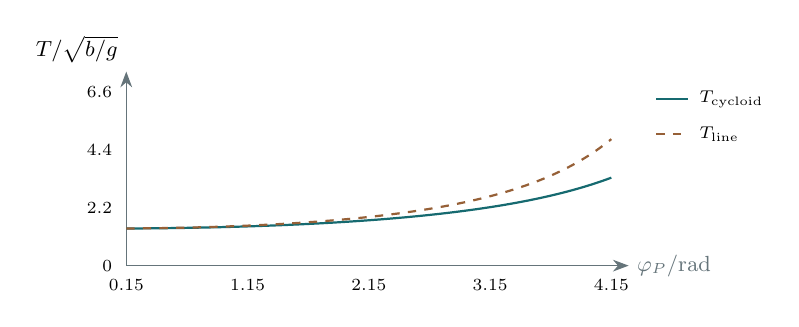
\begin{tikzpicture}[scale=.88,transform shape]
\draw[axis] (0,0.0000000)--(7.25,0.0000000) node[right] {$\varphi_P/\mathrm{rad}$};
\draw[axis] (0.0000000,0)--(0.0000000,2.8);
\node[above left] at (0.0000000,2.8) {$T/\sqrt{b/g}$};
\node[below,font=\scriptsize] at (0.0000000,-0.0800000) {$0.15$};
\node[below,font=\scriptsize] at (1.7500000,-0.0800000) {$1.15$};
\node[below,font=\scriptsize] at (3.5000000,-0.0800000) {$2.15$};
\node[below,font=\scriptsize] at (5.2500000,-0.0800000) {$3.15$};
\node[below,font=\scriptsize] at (7.0000000,-0.0800000) {$4.15$};
\node[left,font=\scriptsize] at (-0.0800000,0.0000000) {$0$};
\node[left,font=\scriptsize] at (-0.0800000,0.8333333) {$2.2$};
\node[left,font=\scriptsize] at (-0.0800000,1.6666667) {$4.4$};
\node[left,font=\scriptsize] at (-0.0800000,2.5000000) {$6.6$};
\draw[thick,color=accent] plot coordinates {(0.0000000,0.5361895) (0.0291667,0.5363075) (0.0583333,0.5364379) (0.0875000,0.5365808) (0.1166667,0.5367362) (0.1458333,0.5369041) (0.1750000,0.5370845) (0.2041667,0.5372775) (0.2333333,0.5374830) (0.2625000,0.5377011) (0.2916667,0.5379317) (0.3208333,0.5381750) (0.3500000,0.5384310) (0.3791667,0.5386996) (0.4083333,0.5389809) (0.4375000,0.5392749) (0.4666667,0.5395817) (0.4958333,0.5399013) (0.5250000,0.5402337) (0.5541667,0.5405789) (0.5833333,0.5409370) (0.6125000,0.5413080) (0.6416667,0.5416920) (0.6708333,0.5420889) (0.7000000,0.5424989) (0.7291667,0.5429219) (0.7583333,0.5433581) (0.7875000,0.5438074) (0.8166667,0.5442700) (0.8458333,0.5447457) (0.8750000,0.5452348) (0.9041667,0.5457372) (0.9333333,0.5462530) (0.9625000,0.5467822) (0.9916667,0.5473250) (1.0208333,0.5478813) (1.0500000,0.5484512) (1.0791667,0.5490348) (1.1083333,0.5496321) (1.1375000,0.5502432) (1.1666667,0.5508681) (1.1958333,0.5515070) (1.2250000,0.5521598) (1.2541667,0.5528267) (1.2833333,0.5535077) (1.3125000,0.5542028) (1.3416667,0.5549123) (1.3708333,0.5556360) (1.4000000,0.5563742) (1.4291667,0.5571268) (1.4583333,0.5578940) (1.4875000,0.5586759) (1.5166667,0.5594724) (1.5458333,0.5602838) (1.5750000,0.5611100) (1.6041667,0.5619513) (1.6333333,0.5628076) (1.6625000,0.5636790) (1.6916667,0.5645657) (1.7208333,0.5654678) (1.7500000,0.5663852) (1.7791667,0.5673183) (1.8083333,0.5682669) (1.8375000,0.5692313) (1.8666667,0.5702115) (1.8958333,0.5712077) (1.9250000,0.5722200) (1.9541667,0.5732484) (1.9833333,0.5742931) (2.0125000,0.5753542) (2.0416667,0.5764318) (2.0708333,0.5775260) (2.1000000,0.5786370) (2.1291667,0.5797648) (2.1583333,0.5809097) (2.1875000,0.5820717) (2.2166667,0.5832509) (2.2458333,0.5844476) (2.2750000,0.5856617) (2.3041667,0.5868935) (2.3333333,0.5881432) (2.3625000,0.5894108) (2.3916667,0.5906964) (2.4208333,0.5920003) (2.4500000,0.5933226) (2.4791667,0.5946635) (2.5083333,0.5960230) (2.5375000,0.5974014) (2.5666667,0.5987989) (2.5958333,0.6002155) (2.6250000,0.6016514) (2.6541667,0.6031069) (2.6833333,0.6045821) (2.7125000,0.6060772) (2.7416667,0.6075923) (2.7708333,0.6091276) (2.8000000,0.6106834) (2.8291667,0.6122598) (2.8583333,0.6138570) (2.8875000,0.6154752) (2.9166667,0.6171146) (2.9458333,0.6187753) (2.9750000,0.6204577) (3.0041667,0.6221620) (3.0333333,0.6238882) (3.0625000,0.6256367) (3.0916667,0.6274077) (3.1208333,0.6292014) (3.1500000,0.6310180) (3.1791667,0.6328578) (3.2083333,0.6347209) (3.2375000,0.6366078) (3.2666667,0.6385185) (3.2958333,0.6404533) (3.3250000,0.6424126) (3.3541667,0.6443965) (3.3833333,0.6464053) (3.4125000,0.6484393) (3.4416667,0.6504988) (3.4708333,0.6525840) (3.5000000,0.6546952) (3.5291667,0.6568328) (3.5583333,0.6589970) (3.5875000,0.6611880) (3.6166667,0.6634063) (3.6458333,0.6656522) (3.6750000,0.6679258) (3.7041667,0.6702276) (3.7333333,0.6725580) (3.7625000,0.6749171) (3.7916667,0.6773054) (3.8208333,0.6797232) (3.8500000,0.6821709) (3.8791667,0.6846488) (3.9083333,0.6871573) (3.9375000,0.6896968) (3.9666667,0.6922676) (3.9958333,0.6948701) (4.0250000,0.6975047) (4.0541667,0.7001719) (4.0833333,0.7028720) (4.1125000,0.7056054) (4.1416667,0.7083726) (4.1708333,0.7111740) (4.2000000,0.7140101) (4.2291667,0.7168812) (4.2583333,0.7197879) (4.2875000,0.7227307) (4.3166667,0.7257099) (4.3458333,0.7287260) (4.3750000,0.7317797) (4.4041667,0.7348713) (4.4333333,0.7380014) (4.4625000,0.7411705) (4.4916667,0.7443792) (4.5208333,0.7476279) (4.5500000,0.7509173) (4.5791667,0.7542479) (4.6083333,0.7576203) (4.6375000,0.7610350) (4.6666667,0.7644927) (4.6958333,0.7679940) (4.7250000,0.7715395) (4.7541667,0.7751299) (4.7833333,0.7787658) (4.8125000,0.7824478) (4.8416667,0.7861767) (4.8708333,0.7899531) (4.9000000,0.7937777) (4.9291667,0.7976513) (4.9583333,0.8015746) (4.9875000,0.8055483) (5.0166667,0.8095733) (5.0458333,0.8136503) (5.0750000,0.8177800) (5.1041667,0.8219634) (5.1333333,0.8262012) (5.1625000,0.8304944) (5.1916667,0.8348437) (5.2208333,0.8392501) (5.2500000,0.8437144) (5.2791667,0.8482377) (5.3083333,0.8528208) (5.3375000,0.8574647) (5.3666667,0.8621705) (5.3958333,0.8669391) (5.4250000,0.8717716) (5.4541667,0.8766691) (5.4833333,0.8816325) (5.5125000,0.8866631) (5.5416667,0.8917620) (5.5708333,0.8969303) (5.6000000,0.9021693) (5.6291667,0.9074801) (5.6583333,0.9128640) (5.6875000,0.9183222) (5.7166667,0.9238561) (5.7458333,0.9294671) (5.7750000,0.9351564) (5.8041667,0.9409255) (5.8333333,0.9467759) (5.8625000,0.9527089) (5.8916667,0.9587261) (5.9208333,0.9648291) (5.9500000,0.9710194) (5.9791667,0.9772987) (6.0083333,0.9836686) (6.0375000,0.9901308) (6.0666667,0.9966871) (6.0958333,1.0033392) (6.1250000,1.0100891) (6.1541667,1.0169385) (6.1833333,1.0238895) (6.2125000,1.0309440) (6.2416667,1.0381040) (6.2708333,1.0453717) (6.3000000,1.0527492) (6.3291667,1.0602387) (6.3583333,1.0678425) (6.3875000,1.0755628) (6.4166667,1.0834022) (6.4458333,1.0913630) (6.4750000,1.0994478) (6.5041667,1.1076592) (6.5333333,1.1159998) (6.5625000,1.1244724) (6.5916667,1.1330798) (6.6208333,1.1418249) (6.6500000,1.1507108) (6.6791667,1.1597404) (6.7083333,1.1689169) (6.7375000,1.1782436) (6.7666667,1.1877239) (6.7958333,1.1973612) (6.8250000,1.2071591) (6.8541667,1.2171212) (6.8833333,1.2272513) (6.9125000,1.2375533) (6.9416667,1.2480313) (6.9708333,1.2586893) (7.0000000,1.2695316)};
\draw[thick,color=accent] (7.65,2.4)--(8.1,2.4);\node[right,font=\scriptsize] at (8.15,2.4) {$T_{\rm cycloid}$};
\draw[thick,dashed,color=warm] plot coordinates {(0.0000000,0.5363572) (0.0291667,0.5365145) (0.0583333,0.5366885) (0.0875000,0.5368792) (0.1166667,0.5370866) (0.1458333,0.5373107) (0.1750000,0.5375515) (0.2041667,0.5378091) (0.2333333,0.5380835) (0.2625000,0.5383748) (0.2916667,0.5386829) (0.3208333,0.5390080) (0.3500000,0.5393500) (0.3791667,0.5397091) (0.4083333,0.5400852) (0.4375000,0.5404784) (0.4666667,0.5408888) (0.4958333,0.5413164) (0.5250000,0.5417612) (0.5541667,0.5422234) (0.5833333,0.5427030) (0.6125000,0.5432000) (0.6416667,0.5437146) (0.6708333,0.5442467) (0.7000000,0.5447965) (0.7291667,0.5453640) (0.7583333,0.5459493) (0.7875000,0.5465526) (0.8166667,0.5471737) (0.8458333,0.5478130) (0.8750000,0.5484703) (0.9041667,0.5491459) (0.9333333,0.5498398) (0.9625000,0.5505522) (0.9916667,0.5512830) (1.0208333,0.5520324) (1.0500000,0.5528005) (1.0791667,0.5535875) (1.1083333,0.5543934) (1.1375000,0.5552183) (1.1666667,0.5560623) (1.1958333,0.5569256) (1.2250000,0.5578083) (1.2541667,0.5587105) (1.2833333,0.5596323) (1.3125000,0.5605738) (1.3416667,0.5615353) (1.3708333,0.5625167) (1.4000000,0.5635184) (1.4291667,0.5645403) (1.4583333,0.5655827) (1.4875000,0.5666456) (1.5166667,0.5677293) (1.5458333,0.5688339) (1.5750000,0.5699596) (1.6041667,0.5711065) (1.6333333,0.5722747) (1.6625000,0.5734645) (1.6916667,0.5746761) (1.7208333,0.5759095) (1.7500000,0.5771650) (1.7791667,0.5784428) (1.8083333,0.5797430) (1.8375000,0.5810658) (1.8666667,0.5824115) (1.8958333,0.5837803) (1.9250000,0.5851723) (1.9541667,0.5865877) (1.9833333,0.5880268) (2.0125000,0.5894897) (2.0416667,0.5909768) (2.0708333,0.5924882) (2.1000000,0.5940242) (2.1291667,0.5955849) (2.1583333,0.5971707) (2.1875000,0.5987817) (2.2166667,0.6004183) (2.2458333,0.6020807) (2.2750000,0.6037691) (2.3041667,0.6054838) (2.3333333,0.6072251) (2.3625000,0.6089933) (2.3916667,0.6107886) (2.4208333,0.6126113) (2.4500000,0.6144618) (2.4791667,0.6163403) (2.5083333,0.6182471) (2.5375000,0.6201825) (2.5666667,0.6221469) (2.5958333,0.6241405) (2.6250000,0.6261638) (2.6541667,0.6282170) (2.6833333,0.6303005) (2.7125000,0.6324147) (2.7416667,0.6345598) (2.7708333,0.6367363) (2.8000000,0.6389445) (2.8291667,0.6411849) (2.8583333,0.6434577) (2.8875000,0.6457635) (2.9166667,0.6481025) (2.9458333,0.6504753) (2.9750000,0.6528822) (3.0041667,0.6553236) (3.0333333,0.6578001) (3.0625000,0.6603119) (3.0916667,0.6628597) (3.1208333,0.6654438) (3.1500000,0.6680648) (3.1791667,0.6707230) (3.2083333,0.6734191) (3.2375000,0.6761535) (3.2666667,0.6789267) (3.2958333,0.6817392) (3.3250000,0.6845916) (3.3541667,0.6874844) (3.3833333,0.6904182) (3.4125000,0.6933936) (3.4416667,0.6964111) (3.4708333,0.6994713) (3.5000000,0.7025748) (3.5291667,0.7057222) (3.5583333,0.7089143) (3.5875000,0.7121515) (3.6166667,0.7154346) (3.6458333,0.7187642) (3.6750000,0.7221410) (3.7041667,0.7255658) (3.7333333,0.7290392) (3.7625000,0.7325619) (3.7916667,0.7361348) (3.8208333,0.7397585) (3.8500000,0.7434339) (3.8791667,0.7471617) (3.9083333,0.7509428) (3.9375000,0.7547779) (3.9666667,0.7586680) (3.9958333,0.7626138) (4.0250000,0.7666163) (4.0541667,0.7706764) (4.0833333,0.7747950) (4.1125000,0.7789731) (4.1416667,0.7832116) (4.1708333,0.7875115) (4.2000000,0.7918737) (4.2291667,0.7962995) (4.2583333,0.8007897) (4.2875000,0.8053456) (4.3166667,0.8099681) (4.3458333,0.8146584) (4.3750000,0.8194177) (4.4041667,0.8242472) (4.4333333,0.8291481) (4.4625000,0.8341216) (4.4916667,0.8391689) (4.5208333,0.8442914) (4.5500000,0.8494905) (4.5791667,0.8547674) (4.6083333,0.8601236) (4.6375000,0.8655605) (4.6666667,0.8710795) (4.6958333,0.8766822) (4.7250000,0.8823701) (4.7541667,0.8881447) (4.7833333,0.8940077) (4.8125000,0.8999607) (4.8416667,0.9060054) (4.8708333,0.9121435) (4.9000000,0.9183769) (4.9291667,0.9247073) (4.9583333,0.9311366) (4.9875000,0.9376667) (5.0166667,0.9442995) (5.0458333,0.9510372) (5.0750000,0.9578817) (5.1041667,0.9648352) (5.1333333,0.9718998) (5.1625000,0.9790778) (5.1916667,0.9863714) (5.2208333,0.9937831) (5.2500000,1.0013152) (5.2791667,1.0089701) (5.3083333,1.0167505) (5.3375000,1.0246590) (5.3666667,1.0326982) (5.3958333,1.0408709) (5.4250000,1.0491798) (5.4541667,1.0576281) (5.4833333,1.0662185) (5.5125000,1.0749542) (5.5416667,1.0838383) (5.5708333,1.0928742) (5.6000000,1.1020650) (5.6291667,1.1114143) (5.6583333,1.1209257) (5.6875000,1.1306026) (5.7166667,1.1404490) (5.7458333,1.1504685) (5.7750000,1.1606652) (5.8041667,1.1710432) (5.8333333,1.1816067) (5.8625000,1.1923600) (5.8916667,1.2033075) (5.9208333,1.2144538) (5.9500000,1.2258038) (5.9791667,1.2373622) (6.0083333,1.2491340) (6.0375000,1.2611245) (6.0666667,1.2733390) (6.0958333,1.2857831) (6.1250000,1.2984623) (6.1541667,1.3113826) (6.1833333,1.3245500) (6.2125000,1.3379708) (6.2416667,1.3516514) (6.2708333,1.3655984) (6.3000000,1.3798189) (6.3291667,1.3943198) (6.3583333,1.4091086) (6.3875000,1.4241927) (6.4166667,1.4395801) (6.4458333,1.4552789) (6.4750000,1.4712975) (6.5041667,1.4876445) (6.5333333,1.5043290) (6.5625000,1.5213601) (6.5916667,1.5387477) (6.6208333,1.5565015) (6.6500000,1.5746320) (6.6791667,1.5931499) (6.7083333,1.6120661) (6.7375000,1.6313922) (6.7666667,1.6511402) (6.7958333,1.6713223) (6.8250000,1.6919514) (6.8541667,1.7130407) (6.8833333,1.7346040) (6.9125000,1.7566558) (6.9416667,1.7792107) (6.9708333,1.8022844) (7.0000000,1.8258927)};
\draw[thick,dashed,color=warm] (7.65,1.9)--(8.1,1.9);\node[right,font=\scriptsize] at (8.15,1.9) {$T_{\rm line}$};
\end{tikzpicture}
\figcaption{变图综二.3V1\quad 同一端点的摆线和直斜面时间}
\end{minipage}\end{center}
\item \textbf{接近竖直的终点。}令$a/b$很小，估计末相位和时间。分子、分母的首项分别为$\varphi_P^3/6$与$\varphi_P^2/2$，故
\[
\varphi_P\simeq 3a/b,\qquad
T_{\min}=\sqrt{2b/g}\frac{\varphi_P}{2\sin(\varphi_P/2)}
\longrightarrow\sqrt{2b/g}.
\]
图V2中实线与斜率3的虚线在小比例处接近。展开时间因子还得$1+\varphi_P^2/24+O(\varphi_P^4)$，横向距离的一阶小量只改变末相位，时间从二阶才偏离竖直自由落体值。
\begin{center}\begin{minipage}{.98\linewidth}\centering
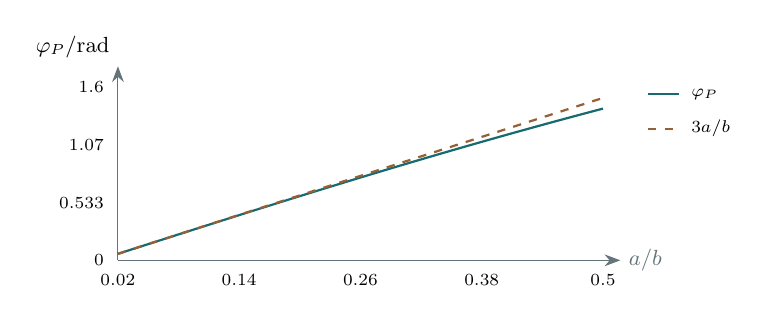
\begin{tikzpicture}[scale=.88,transform shape]
\draw[axis] (0,0.0000000)--(7.25,0.0000000) node[right] {$a/b$};
\draw[axis] (0.0000000,0)--(0.0000000,2.8);
\node[above left] at (0.0000000,2.8) {$\varphi_P/\mathrm{rad}$};
\node[below,font=\scriptsize] at (0.0000000,-0.0800000) {$0.02$};
\node[below,font=\scriptsize] at (1.7500000,-0.0800000) {$0.14$};
\node[below,font=\scriptsize] at (3.5000000,-0.0800000) {$0.26$};
\node[below,font=\scriptsize] at (5.2500000,-0.0800000) {$0.38$};
\node[below,font=\scriptsize] at (7.0000000,-0.0800000) {$0.5$};
\node[left,font=\scriptsize] at (-0.0800000,0.0000000) {$0$};
\node[left,font=\scriptsize] at (-0.0800000,0.8333333) {$0.533$};
\node[left,font=\scriptsize] at (-0.0800000,1.6666667) {$1.07$};
\node[left,font=\scriptsize] at (-0.0800000,2.5000000) {$1.6$};
\draw[thick,color=accent] plot coordinates {(0.0000000,0.0937388) (0.0291667,0.1031100) (0.0583333,0.1124806) (0.0875000,0.1218503) (0.1166667,0.1312191) (0.1458333,0.1405871) (0.1750000,0.1499539) (0.2041667,0.1593198) (0.2333333,0.1686844) (0.2625000,0.1780479) (0.2916667,0.1874101) (0.3208333,0.1967709) (0.3500000,0.2061303) (0.3791667,0.2154883) (0.4083333,0.2248447) (0.4375000,0.2341995) (0.4666667,0.2435526) (0.4958333,0.2529039) (0.5250000,0.2622535) (0.5541667,0.2716012) (0.5833333,0.2809469) (0.6125000,0.2902906) (0.6416667,0.2996322) (0.6708333,0.3089717) (0.7000000,0.3183090) (0.7291667,0.3276440) (0.7583333,0.3369767) (0.7875000,0.3463070) (0.8166667,0.3556347) (0.8458333,0.3649600) (0.8750000,0.3742827) (0.9041667,0.3836026) (0.9333333,0.3929199) (0.9625000,0.4022344) (0.9916667,0.4115460) (1.0208333,0.4208546) (1.0500000,0.4301603) (1.0791667,0.4394629) (1.1083333,0.4487624) (1.1375000,0.4580588) (1.1666667,0.4673518) (1.1958333,0.4766416) (1.2250000,0.4859280) (1.2541667,0.4952109) (1.2833333,0.5044904) (1.3125000,0.5137663) (1.3416667,0.5230385) (1.3708333,0.5323071) (1.4000000,0.5415719) (1.4291667,0.5508329) (1.4583333,0.5600900) (1.4875000,0.5693432) (1.5166667,0.5785924) (1.5458333,0.5878375) (1.5750000,0.5970785) (1.6041667,0.6063153) (1.6333333,0.6155479) (1.6625000,0.6247761) (1.6916667,0.6340000) (1.7208333,0.6432195) (1.7500000,0.6524344) (1.7791667,0.6616448) (1.8083333,0.6708506) (1.8375000,0.6800517) (1.8666667,0.6892481) (1.8958333,0.6984397) (1.9250000,0.7076265) (1.9541667,0.7168083) (1.9833333,0.7259852) (2.0125000,0.7351571) (2.0416667,0.7443238) (2.0708333,0.7534854) (2.1000000,0.7626419) (2.1291667,0.7717930) (2.1583333,0.7809389) (2.1875000,0.7900793) (2.2166667,0.7992144) (2.2458333,0.8083439) (2.2750000,0.8174679) (2.3041667,0.8265863) (2.3333333,0.8356991) (2.3625000,0.8448061) (2.3916667,0.8539074) (2.4208333,0.8630028) (2.4500000,0.8720924) (2.4791667,0.8811760) (2.5083333,0.8902537) (2.5375000,0.8993253) (2.5666667,0.9083908) (2.5958333,0.9174501) (2.6250000,0.9265033) (2.6541667,0.9355502) (2.6833333,0.9445908) (2.7125000,0.9536250) (2.7416667,0.9626528) (2.7708333,0.9716741) (2.8000000,0.9806889) (2.8291667,0.9896971) (2.8583333,0.9986987) (2.8875000,1.0076937) (2.9166667,1.0166819) (2.9458333,1.0256633) (2.9750000,1.0346379) (3.0041667,1.0436056) (3.0333333,1.0525664) (3.0625000,1.0615202) (3.0916667,1.0704670) (3.1208333,1.0794067) (3.1500000,1.0883393) (3.1791667,1.0972647) (3.2083333,1.1061828) (3.2375000,1.1150937) (3.2666667,1.1239973) (3.2958333,1.1328936) (3.3250000,1.1417824) (3.3541667,1.1506637) (3.3833333,1.1595376) (3.4125000,1.1684039) (3.4416667,1.1772625) (3.4708333,1.1861136) (3.5000000,1.1949569) (3.5291667,1.2037926) (3.5583333,1.2126204) (3.5875000,1.2214404) (3.6166667,1.2302526) (3.6458333,1.2390568) (3.6750000,1.2478531) (3.7041667,1.2566414) (3.7333333,1.2654216) (3.7625000,1.2741937) (3.7916667,1.2829578) (3.8208333,1.2917136) (3.8500000,1.3004613) (3.8791667,1.3092006) (3.9083333,1.3179317) (3.9375000,1.3266545) (3.9666667,1.3353689) (3.9958333,1.3440748) (4.0250000,1.3527723) (4.0541667,1.3614613) (4.0833333,1.3701418) (4.1125000,1.3788137) (4.1416667,1.3874770) (4.1708333,1.3961316) (4.2000000,1.4047775) (4.2291667,1.4134147) (4.2583333,1.4220432) (4.2875000,1.4306628) (4.3166667,1.4392736) (4.3458333,1.4478755) (4.3750000,1.4564686) (4.4041667,1.4650526) (4.4333333,1.4736277) (4.4625000,1.4821937) (4.4916667,1.4907507) (4.5208333,1.4992986) (4.5500000,1.5078374) (4.5791667,1.5163670) (4.6083333,1.5248875) (4.6375000,1.5333986) (4.6666667,1.5419006) (4.6958333,1.5503932) (4.7250000,1.5588765) (4.7541667,1.5673505) (4.7833333,1.5758151) (4.8125000,1.5842702) (4.8416667,1.5927159) (4.8708333,1.6011521) (4.9000000,1.6095788) (4.9291667,1.6179959) (4.9583333,1.6264035) (4.9875000,1.6348015) (5.0166667,1.6431898) (5.0458333,1.6515684) (5.0750000,1.6599374) (5.1041667,1.6682966) (5.1333333,1.6766461) (5.1625000,1.6849858) (5.1916667,1.6933157) (5.2208333,1.7016358) (5.2500000,1.7099460) (5.2791667,1.7182463) (5.3083333,1.7265367) (5.3375000,1.7348171) (5.3666667,1.7430876) (5.3958333,1.7513481) (5.4250000,1.7595986) (5.4541667,1.7678390) (5.4833333,1.7760694) (5.5125000,1.7842896) (5.5416667,1.7924998) (5.5708333,1.8006998) (5.6000000,1.8088896) (5.6291667,1.8170693) (5.6583333,1.8252387) (5.6875000,1.8333979) (5.7166667,1.8415468) (5.7458333,1.8496855) (5.7750000,1.8578139) (5.8041667,1.8659319) (5.8333333,1.8740396) (5.8625000,1.8821369) (5.8916667,1.8902239) (5.9208333,1.8983004) (5.9500000,1.9063665) (5.9791667,1.9144222) (6.0083333,1.9224674) (6.0375000,1.9305021) (6.0666667,1.9385263) (6.0958333,1.9465400) (6.1250000,1.9545431) (6.1541667,1.9625357) (6.1833333,1.9705177) (6.2125000,1.9784892) (6.2416667,1.9864500) (6.2708333,1.9944001) (6.3000000,2.0023396) (6.3291667,2.0102685) (6.3583333,2.0181867) (6.3875000,2.0260942) (6.4166667,2.0339910) (6.4458333,2.0418770) (6.4750000,2.0497523) (6.5041667,2.0576169) (6.5333333,2.0654706) (6.5625000,2.0733136) (6.5916667,2.0811458) (6.6208333,2.0889672) (6.6500000,2.0967778) (6.6791667,2.1045775) (6.7083333,2.1123664) (6.7375000,2.1201444) (6.7666667,2.1279115) (6.7958333,2.1356677) (6.8250000,2.1434130) (6.8541667,2.1511474) (6.8833333,2.1588709) (6.9125000,2.1665835) (6.9416667,2.1742851) (6.9708333,2.1819757) (7.0000000,2.1896554)};
\draw[thick,color=accent] (7.65,2.4)--(8.1,2.4);\node[right,font=\scriptsize] at (8.15,2.4) {$\varphi_P$};
\draw[thick,dashed,color=warm] plot coordinates {(0.0000000,0.0937500) (0.0291667,0.1031250) (0.0583333,0.1125000) (0.0875000,0.1218750) (0.1166667,0.1312500) (0.1458333,0.1406250) (0.1750000,0.1500000) (0.2041667,0.1593750) (0.2333333,0.1687500) (0.2625000,0.1781250) (0.2916667,0.1875000) (0.3208333,0.1968750) (0.3500000,0.2062500) (0.3791667,0.2156250) (0.4083333,0.2250000) (0.4375000,0.2343750) (0.4666667,0.2437500) (0.4958333,0.2531250) (0.5250000,0.2625000) (0.5541667,0.2718750) (0.5833333,0.2812500) (0.6125000,0.2906250) (0.6416667,0.3000000) (0.6708333,0.3093750) (0.7000000,0.3187500) (0.7291667,0.3281250) (0.7583333,0.3375000) (0.7875000,0.3468750) (0.8166667,0.3562500) (0.8458333,0.3656250) (0.8750000,0.3750000) (0.9041667,0.3843750) (0.9333333,0.3937500) (0.9625000,0.4031250) (0.9916667,0.4125000) (1.0208333,0.4218750) (1.0500000,0.4312500) (1.0791667,0.4406250) (1.1083333,0.4500000) (1.1375000,0.4593750) (1.1666667,0.4687500) (1.1958333,0.4781250) (1.2250000,0.4875000) (1.2541667,0.4968750) (1.2833333,0.5062500) (1.3125000,0.5156250) (1.3416667,0.5250000) (1.3708333,0.5343750) (1.4000000,0.5437500) (1.4291667,0.5531250) (1.4583333,0.5625000) (1.4875000,0.5718750) (1.5166667,0.5812500) (1.5458333,0.5906250) (1.5750000,0.6000000) (1.6041667,0.6093750) (1.6333333,0.6187500) (1.6625000,0.6281250) (1.6916667,0.6375000) (1.7208333,0.6468750) (1.7500000,0.6562500) (1.7791667,0.6656250) (1.8083333,0.6750000) (1.8375000,0.6843750) (1.8666667,0.6937500) (1.8958333,0.7031250) (1.9250000,0.7125000) (1.9541667,0.7218750) (1.9833333,0.7312500) (2.0125000,0.7406250) (2.0416667,0.7500000) (2.0708333,0.7593750) (2.1000000,0.7687500) (2.1291667,0.7781250) (2.1583333,0.7875000) (2.1875000,0.7968750) (2.2166667,0.8062500) (2.2458333,0.8156250) (2.2750000,0.8250000) (2.3041667,0.8343750) (2.3333333,0.8437500) (2.3625000,0.8531250) (2.3916667,0.8625000) (2.4208333,0.8718750) (2.4500000,0.8812500) (2.4791667,0.8906250) (2.5083333,0.9000000) (2.5375000,0.9093750) (2.5666667,0.9187500) (2.5958333,0.9281250) (2.6250000,0.9375000) (2.6541667,0.9468750) (2.6833333,0.9562500) (2.7125000,0.9656250) (2.7416667,0.9750000) (2.7708333,0.9843750) (2.8000000,0.9937500) (2.8291667,1.0031250) (2.8583333,1.0125000) (2.8875000,1.0218750) (2.9166667,1.0312500) (2.9458333,1.0406250) (2.9750000,1.0500000) (3.0041667,1.0593750) (3.0333333,1.0687500) (3.0625000,1.0781250) (3.0916667,1.0875000) (3.1208333,1.0968750) (3.1500000,1.1062500) (3.1791667,1.1156250) (3.2083333,1.1250000) (3.2375000,1.1343750) (3.2666667,1.1437500) (3.2958333,1.1531250) (3.3250000,1.1625000) (3.3541667,1.1718750) (3.3833333,1.1812500) (3.4125000,1.1906250) (3.4416667,1.2000000) (3.4708333,1.2093750) (3.5000000,1.2187500) (3.5291667,1.2281250) (3.5583333,1.2375000) (3.5875000,1.2468750) (3.6166667,1.2562500) (3.6458333,1.2656250) (3.6750000,1.2750000) (3.7041667,1.2843750) (3.7333333,1.2937500) (3.7625000,1.3031250) (3.7916667,1.3125000) (3.8208333,1.3218750) (3.8500000,1.3312500) (3.8791667,1.3406250) (3.9083333,1.3500000) (3.9375000,1.3593750) (3.9666667,1.3687500) (3.9958333,1.3781250) (4.0250000,1.3875000) (4.0541667,1.3968750) (4.0833333,1.4062500) (4.1125000,1.4156250) (4.1416667,1.4250000) (4.1708333,1.4343750) (4.2000000,1.4437500) (4.2291667,1.4531250) (4.2583333,1.4625000) (4.2875000,1.4718750) (4.3166667,1.4812500) (4.3458333,1.4906250) (4.3750000,1.5000000) (4.4041667,1.5093750) (4.4333333,1.5187500) (4.4625000,1.5281250) (4.4916667,1.5375000) (4.5208333,1.5468750) (4.5500000,1.5562500) (4.5791667,1.5656250) (4.6083333,1.5750000) (4.6375000,1.5843750) (4.6666667,1.5937500) (4.6958333,1.6031250) (4.7250000,1.6125000) (4.7541667,1.6218750) (4.7833333,1.6312500) (4.8125000,1.6406250) (4.8416667,1.6500000) (4.8708333,1.6593750) (4.9000000,1.6687500) (4.9291667,1.6781250) (4.9583333,1.6875000) (4.9875000,1.6968750) (5.0166667,1.7062500) (5.0458333,1.7156250) (5.0750000,1.7250000) (5.1041667,1.7343750) (5.1333333,1.7437500) (5.1625000,1.7531250) (5.1916667,1.7625000) (5.2208333,1.7718750) (5.2500000,1.7812500) (5.2791667,1.7906250) (5.3083333,1.8000000) (5.3375000,1.8093750) (5.3666667,1.8187500) (5.3958333,1.8281250) (5.4250000,1.8375000) (5.4541667,1.8468750) (5.4833333,1.8562500) (5.5125000,1.8656250) (5.5416667,1.8750000) (5.5708333,1.8843750) (5.6000000,1.8937500) (5.6291667,1.9031250) (5.6583333,1.9125000) (5.6875000,1.9218750) (5.7166667,1.9312500) (5.7458333,1.9406250) (5.7750000,1.9500000) (5.8041667,1.9593750) (5.8333333,1.9687500) (5.8625000,1.9781250) (5.8916667,1.9875000) (5.9208333,1.9968750) (5.9500000,2.0062500) (5.9791667,2.0156250) (6.0083333,2.0250000) (6.0375000,2.0343750) (6.0666667,2.0437500) (6.0958333,2.0531250) (6.1250000,2.0625000) (6.1541667,2.0718750) (6.1833333,2.0812500) (6.2125000,2.0906250) (6.2416667,2.1000000) (6.2708333,2.1093750) (6.3000000,2.1187500) (6.3291667,2.1281250) (6.3583333,2.1375000) (6.3875000,2.1468750) (6.4166667,2.1562500) (6.4458333,2.1656250) (6.4750000,2.1750000) (6.5041667,2.1843750) (6.5333333,2.1937500) (6.5625000,2.2031250) (6.5916667,2.2125000) (6.6208333,2.2218750) (6.6500000,2.2312500) (6.6791667,2.2406250) (6.7083333,2.2500000) (6.7375000,2.2593750) (6.7666667,2.2687500) (6.7958333,2.2781250) (6.8250000,2.2875000) (6.8541667,2.2968750) (6.8833333,2.3062500) (6.9125000,2.3156250) (6.9416667,2.3250000) (6.9708333,2.3343750) (7.0000000,2.3437500)};
\draw[thick,dashed,color=warm] (7.65,1.9)--(8.1,1.9);\node[right,font=\scriptsize] at (8.15,1.9) {$3a/b$};
\end{tikzpicture}
\figcaption{变图综二.3V2\quad 小横向偏移时的端点参数}
\end{minipage}\end{center}
\item \textbf{计算下降过头的距离。}取末相位$3\pi/2$，求终点比例和轨道最低点。此时$1-\cos\varphi_P=1$，$\sin\varphi_P=-1$，故
\[
a/b=3\pi/2+1,\qquad
\mathcal R=b,\qquad
y_{\max}=2\mathcal R=2b.
\]
图V3的曲线从$y_{\max}/b=1$开始，$\varphi_P=3\pi/2$时纵坐标为2。轨道先下落$2b$，末段上升$b$才到$P$。
\begin{center}\begin{minipage}{.98\linewidth}\centering
\begin{tikzpicture}[scale=.88,transform shape]
\draw[axis] (0,0.0000000)--(7.25,0.0000000) node[right] {$\varphi_P/\mathrm{rad}$};
\draw[axis] (0.0000000,0)--(0.0000000,2.8);
\node[above left] at (0.0000000,2.8) {$y_{\max}/b$};
\node[below,font=\scriptsize] at (0.0000000,-0.0800000) {$3.14$};
\node[below,font=\scriptsize] at (1.7500000,-0.0800000) {$3.71$};
\node[below,font=\scriptsize] at (3.5000000,-0.0800000) {$4.27$};
\node[below,font=\scriptsize] at (5.2500000,-0.0800000) {$4.84$};
\node[below,font=\scriptsize] at (7.0000000,-0.0800000) {$5.4$};
\node[left,font=\scriptsize] at (-0.0800000,0.0000000) {$0$};
\node[left,font=\scriptsize] at (-0.0800000,0.8333333) {$2$};
\node[left,font=\scriptsize] at (-0.0800000,1.6666667) {$4$};
\node[left,font=\scriptsize] at (-0.0800000,2.5000000) {$6$};
\draw[thick,color=accent] plot coordinates {(0.0000000,0.4166667) (0.0291667,0.4166759) (0.0583333,0.4167036) (0.0875000,0.4167497) (0.1166667,0.4168143) (0.1458333,0.4168973) (0.1750000,0.4169989) (0.2041667,0.4171190) (0.2333333,0.4172575) (0.2625000,0.4174147) (0.2916667,0.4175904) (0.3208333,0.4177847) (0.3500000,0.4179977) (0.3791667,0.4182294) (0.4083333,0.4184798) (0.4375000,0.4187489) (0.4666667,0.4190369) (0.4958333,0.4193438) (0.5250000,0.4196695) (0.5541667,0.4200143) (0.5833333,0.4203781) (0.6125000,0.4207610) (0.6416667,0.4211631) (0.6708333,0.4215844) (0.7000000,0.4220251) (0.7291667,0.4224851) (0.7583333,0.4229647) (0.7875000,0.4234638) (0.8166667,0.4239826) (0.8458333,0.4245212) (0.8750000,0.4250796) (0.9041667,0.4256580) (0.9333333,0.4262565) (0.9625000,0.4268751) (0.9916667,0.4275140) (1.0208333,0.4281733) (1.0500000,0.4288532) (1.0791667,0.4295537) (1.1083333,0.4302749) (1.1375000,0.4310171) (1.1666667,0.4317804) (1.1958333,0.4325648) (1.2250000,0.4333706) (1.2541667,0.4341979) (1.2833333,0.4350469) (1.3125000,0.4359176) (1.3416667,0.4368104) (1.3708333,0.4377252) (1.4000000,0.4386624) (1.4291667,0.4396221) (1.4583333,0.4406045) (1.4875000,0.4416097) (1.5166667,0.4426380) (1.5458333,0.4436896) (1.5750000,0.4447646) (1.6041667,0.4458633) (1.6333333,0.4469859) (1.6625000,0.4481326) (1.6916667,0.4493037) (1.7208333,0.4504993) (1.7500000,0.4517197) (1.7791667,0.4529652) (1.8083333,0.4542360) (1.8375000,0.4555323) (1.8666667,0.4568544) (1.8958333,0.4582026) (1.9250000,0.4595772) (1.9541667,0.4609784) (1.9833333,0.4624065) (2.0125000,0.4638618) (2.0416667,0.4653447) (2.0708333,0.4668553) (2.1000000,0.4683942) (2.1291667,0.4699614) (2.1583333,0.4715575) (2.1875000,0.4731827) (2.2166667,0.4748374) (2.2458333,0.4765219) (2.2750000,0.4782366) (2.3041667,0.4799818) (2.3333333,0.4817580) (2.3625000,0.4835655) (2.3916667,0.4854048) (2.4208333,0.4872761) (2.4500000,0.4891801) (2.4791667,0.4911169) (2.5083333,0.4930872) (2.5375000,0.4950913) (2.5666667,0.4971298) (2.5958333,0.4992029) (2.6250000,0.5013114) (2.6541667,0.5034555) (2.6833333,0.5056359) (2.7125000,0.5078530) (2.7416667,0.5101073) (2.7708333,0.5123994) (2.8000000,0.5147299) (2.8291667,0.5170992) (2.8583333,0.5195080) (2.8875000,0.5219568) (2.9166667,0.5244462) (2.9458333,0.5269769) (2.9750000,0.5295494) (3.0041667,0.5321645) (3.0333333,0.5348227) (3.0625000,0.5375247) (3.0916667,0.5402712) (3.1208333,0.5430630) (3.1500000,0.5459006) (3.1791667,0.5487850) (3.2083333,0.5517167) (3.2375000,0.5546966) (3.2666667,0.5577255) (3.2958333,0.5608042) (3.3250000,0.5639334) (3.3541667,0.5671141) (3.3833333,0.5703471) (3.4125000,0.5736333) (3.4416667,0.5769736) (3.4708333,0.5803690) (3.5000000,0.5838203) (3.5291667,0.5873286) (3.5583333,0.5908948) (3.5875000,0.5945200) (3.6166667,0.5982053) (3.6458333,0.6019516) (3.6750000,0.6057602) (3.7041667,0.6096321) (3.7333333,0.6135685) (3.7625000,0.6175706) (3.7916667,0.6216395) (3.8208333,0.6257766) (3.8500000,0.6299832) (3.8791667,0.6342604) (3.9083333,0.6386098) (3.9375000,0.6430326) (3.9666667,0.6475303) (3.9958333,0.6521043) (4.0250000,0.6567561) (4.0541667,0.6614873) (4.0833333,0.6662993) (4.1125000,0.6711939) (4.1416667,0.6761727) (4.1708333,0.6812374) (4.2000000,0.6863897) (4.2291667,0.6916314) (4.2583333,0.6969643) (4.2875000,0.7023904) (4.3166667,0.7079115) (4.3458333,0.7135298) (4.3750000,0.7192471) (4.4041667,0.7250657) (4.4333333,0.7309876) (4.4625000,0.7370152) (4.4916667,0.7431507) (4.5208333,0.7493964) (4.5500000,0.7557548) (4.5791667,0.7622283) (4.6083333,0.7688196) (4.6375000,0.7755312) (4.6666667,0.7823659) (4.6958333,0.7893264) (4.7250000,0.7964157) (4.7541667,0.8036366) (4.7833333,0.8109923) (4.8125000,0.8184858) (4.8416667,0.8261204) (4.8708333,0.8338994) (4.9000000,0.8418262) (4.9291667,0.8499044) (4.9583333,0.8581377) (4.9875000,0.8665297) (5.0166667,0.8750843) (5.0458333,0.8838056) (5.0750000,0.8926976) (5.1041667,0.9017647) (5.1333333,0.9110111) (5.1625000,0.9204414) (5.1916667,0.9300603) (5.2208333,0.9398726) (5.2500000,0.9498833) (5.2791667,0.9600975) (5.3083333,0.9705205) (5.3375000,0.9811579) (5.3666667,0.9920153) (5.3958333,1.0030986) (5.4250000,1.0144138) (5.4541667,1.0259672) (5.4833333,1.0377654) (5.5125000,1.0498150) (5.5416667,1.0621230) (5.5708333,1.0746966) (5.6000000,1.0875432) (5.6291667,1.1006705) (5.6583333,1.1140866) (5.6875000,1.1277998) (5.7166667,1.1418185) (5.7458333,1.1561518) (5.7750000,1.1708089) (5.8041667,1.1857992) (5.8333333,1.2011329) (5.8625000,1.2168201) (5.8916667,1.2328716) (5.9208333,1.2492985) (5.9500000,1.2661123) (5.9791667,1.2833251) (6.0083333,1.3009493) (6.0375000,1.3189978) (6.0666667,1.3374842) (6.0958333,1.3564225) (6.1250000,1.3758271) (6.1541667,1.3957135) (6.1833333,1.4160972) (6.2125000,1.4369949) (6.2416667,1.4584237) (6.2708333,1.4804014) (6.3000000,1.5029467) (6.3291667,1.5260791) (6.3583333,1.5498188) (6.3875000,1.5741870) (6.4166667,1.5992059) (6.4458333,1.6248985) (6.4750000,1.6512890) (6.5041667,1.6784025) (6.5333333,1.7062656) (6.5625000,1.7349057) (6.5916667,1.7643518) (6.6208333,1.7946341) (6.6500000,1.8257844) (6.6791667,1.8578357) (6.7083333,1.8908229) (6.7375000,1.9247825) (6.7666667,1.9597529) (6.7958333,1.9957741) (6.8250000,2.0328886) (6.8541667,2.0711406) (6.8833333,2.1105769) (6.9125000,2.1512464) (6.9416667,2.1932010) (6.9708333,2.2364949) (7.0000000,2.2811856)};
\end{tikzpicture}
\figcaption{变图综二.3V3\quad 上升段越长，最低点越深于终点}
\end{minipage}\end{center}
\item \textbf{缩小轨道或加强重力。}长度整体乘$\lambda$时，$a/b$和末相位保持相同，$\mathcal R$乘$\lambda$。固定几何而令$g$乘$\lambda$时，$\mathcal R$保持相同。代入时间式得
\[
T_{\rm length}^\prime/T=\sqrt\lambda,\qquad
T_g^\prime/T=1/\sqrt\lambda.
\]
图V4中实线在$\lambda=1/4$处给半时，虚线在$\lambda=4$处也给半时。把所有长度缩为四分之一，同时把$g$增至四倍，两个时间因子相乘，得到原时间的$1/4$。
\begin{center}\begin{minipage}{.98\linewidth}\centering
\begin{tikzpicture}[scale=.88,transform shape]
\draw[axis] (0,0.0000000)--(7.25,0.0000000) node[right] {$\lambda$};
\draw[axis] (0.0000000,0)--(0.0000000,2.8);
\node[above left] at (0.0000000,2.8) {$T^\prime/T$};
\node[below,font=\scriptsize] at (0.0000000,-0.0800000) {$0.25$};
\node[below,font=\scriptsize] at (1.7500000,-0.0800000) {$1.19$};
\node[below,font=\scriptsize] at (3.5000000,-0.0800000) {$2.12$};
\node[below,font=\scriptsize] at (5.2500000,-0.0800000) {$3.06$};
\node[below,font=\scriptsize] at (7.0000000,-0.0800000) {$4$};
\node[left,font=\scriptsize] at (-0.0800000,0.0000000) {$0$};
\node[left,font=\scriptsize] at (-0.0800000,0.8333333) {$0.733$};
\node[left,font=\scriptsize] at (-0.0800000,1.6666667) {$1.47$};
\node[left,font=\scriptsize] at (-0.0800000,2.5000000) {$2.2$};
\draw[thick,color=accent] plot coordinates {(0.0000000,0.5681818) (0.0291667,0.5856684) (0.0583333,0.6026478) (0.0875000,0.6191618) (0.1166667,0.6352466) (0.1458333,0.6509340) (0.1750000,0.6662522) (0.2041667,0.6812261) (0.2333333,0.6958778) (0.2625000,0.7102273) (0.2916667,0.7242925) (0.3208333,0.7380898) (0.3500000,0.7516339) (0.3791667,0.7649382) (0.4083333,0.7780150) (0.4375000,0.7908756) (0.4666667,0.8035304) (0.4958333,0.8159890) (0.5250000,0.8282602) (0.5541667,0.8403522) (0.5833333,0.8522727) (0.6125000,0.8640288) (0.6416667,0.8756270) (0.6708333,0.8870736) (0.7000000,0.8983743) (0.7291667,0.9095347) (0.7583333,0.9205598) (0.7875000,0.9314543) (0.8166667,0.9422230) (0.8458333,0.9528699) (0.8750000,0.9633991) (0.9041667,0.9738146) (0.9333333,0.9841198) (0.9625000,0.9943182) (0.9916667,1.0044130) (1.0208333,1.0144074) (1.0500000,1.0243043) (1.0791667,1.0341065) (1.1083333,1.0438167) (1.1375000,1.0534373) (1.1666667,1.0629708) (1.1958333,1.0724197) (1.2250000,1.0817860) (1.2541667,1.0910718) (1.2833333,1.1002794) (1.3125000,1.1094105) (1.3416667,1.1184670) (1.3708333,1.1274508) (1.4000000,1.1363636) (1.4291667,1.1452071) (1.4583333,1.1539827) (1.4875000,1.1626922) (1.5166667,1.1713368) (1.5458333,1.1799182) (1.5750000,1.1884375) (1.6041667,1.1968963) (1.6333333,1.2052956) (1.6625000,1.2136369) (1.6916667,1.2219212) (1.7208333,1.2301497) (1.7500000,1.2383236) (1.7791667,1.2464438) (1.8083333,1.2545115) (1.8375000,1.2625276) (1.8666667,1.2704932) (1.8958333,1.2784091) (1.9250000,1.2862763) (1.9541667,1.2940957) (1.9833333,1.3018681) (2.0125000,1.3095944) (2.0416667,1.3172754) (2.0708333,1.3249118) (2.1000000,1.3325045) (2.1291667,1.3400541) (2.1583333,1.3475615) (2.1875000,1.3550273) (2.2166667,1.3624521) (2.2458333,1.3698368) (2.2750000,1.3771818) (2.3041667,1.3844878) (2.3333333,1.3917555) (2.3625000,1.3989855) (2.3916667,1.4061783) (2.4208333,1.4133344) (2.4500000,1.4204545) (2.4791667,1.4275392) (2.5083333,1.4345888) (2.5375000,1.4416039) (2.5666667,1.4485851) (2.5958333,1.4555328) (2.6250000,1.4624475) (2.6541667,1.4693296) (2.6833333,1.4761797) (2.7125000,1.4829981) (2.7416667,1.4897853) (2.7708333,1.4965417) (2.8000000,1.5032678) (2.8291667,1.5099639) (2.8583333,1.5166304) (2.8875000,1.5232678) (2.9166667,1.5298764) (2.9458333,1.5364565) (2.9750000,1.5430086) (3.0041667,1.5495330) (3.0333333,1.5560300) (3.0625000,1.5625000) (3.0916667,1.5689433) (3.1208333,1.5753603) (3.1500000,1.5817512) (3.1791667,1.5881165) (3.2083333,1.5944563) (3.2375000,1.6007710) (3.2666667,1.6070609) (3.2958333,1.6133262) (3.3250000,1.6195674) (3.3541667,1.6257845) (3.3833333,1.6319780) (3.4125000,1.6381481) (3.4416667,1.6442950) (3.4708333,1.6504190) (3.5000000,1.6565204) (3.5291667,1.6625994) (3.5583333,1.6686563) (3.5875000,1.6746912) (3.6166667,1.6807045) (3.6458333,1.6866963) (3.6750000,1.6926669) (3.7041667,1.6986166) (3.7333333,1.7045455) (3.7625000,1.7104538) (3.7916667,1.7163418) (3.8208333,1.7222096) (3.8500000,1.7280575) (3.8791667,1.7338857) (3.9083333,1.7396944) (3.9375000,1.7454838) (3.9666667,1.7512540) (3.9958333,1.7570052) (4.0250000,1.7627377) (4.0541667,1.7684516) (4.0833333,1.7741472) (4.1125000,1.7798244) (4.1416667,1.7854837) (4.1708333,1.7911250) (4.2000000,1.7967487) (4.2291667,1.8023548) (4.2583333,1.8079435) (4.2875000,1.8135150) (4.3166667,1.8190694) (4.3458333,1.8246069) (4.3750000,1.8301277) (4.4041667,1.8356318) (4.4333333,1.8411195) (4.4625000,1.8465909) (4.4916667,1.8520461) (4.5208333,1.8574853) (4.5500000,1.8629087) (4.5791667,1.8683163) (4.6083333,1.8737082) (4.6375000,1.8790847) (4.6666667,1.8844459) (4.6958333,1.8897919) (4.7250000,1.8951227) (4.7541667,1.9004387) (4.7833333,1.9057398) (4.8125000,1.9110261) (4.8416667,1.9162979) (4.8708333,1.9215553) (4.9000000,1.9267983) (4.9291667,1.9320271) (4.9583333,1.9372417) (4.9875000,1.9424424) (5.0166667,1.9476291) (5.0458333,1.9528021) (5.0750000,1.9579615) (5.1041667,1.9631072) (5.1333333,1.9682396) (5.1625000,1.9733585) (5.1916667,1.9784642) (5.2208333,1.9835568) (5.2500000,1.9886364) (5.2791667,1.9937030) (5.3083333,1.9987567) (5.3375000,2.0037977) (5.3666667,2.0088261) (5.3958333,2.0138419) (5.4250000,2.0188452) (5.4541667,2.0238362) (5.4833333,2.0288149) (5.5125000,2.0337814) (5.5416667,2.0387358) (5.5708333,2.0436782) (5.6000000,2.0486087) (5.6291667,2.0535273) (5.6583333,2.0584342) (5.6875000,2.0633294) (5.7166667,2.0682130) (5.7458333,2.0730852) (5.7750000,2.0779459) (5.8041667,2.0827952) (5.8333333,2.0876333) (5.8625000,2.0924602) (5.8916667,2.0972760) (5.9208333,2.1020808) (5.9500000,2.1068746) (5.9791667,2.1116575) (6.0083333,2.1164296) (6.0375000,2.1211910) (6.0666667,2.1259417) (6.0958333,2.1306818) (6.1250000,2.1354114) (6.1541667,2.1401306) (6.1833333,2.1448393) (6.2125000,2.1495378) (6.2416667,2.1542260) (6.2708333,2.1589040) (6.3000000,2.1635719) (6.3291667,2.1682298) (6.3583333,2.1728776) (6.3875000,2.1775156) (6.4166667,2.1821437) (6.4458333,2.1867620) (6.4750000,2.1913705) (6.5041667,2.1959694) (6.5333333,2.2005587) (6.5625000,2.2051385) (6.5916667,2.2097087) (6.6208333,2.2142695) (6.6500000,2.2188209) (6.6791667,2.2233630) (6.7083333,2.2278959) (6.7375000,2.2324196) (6.7666667,2.2369341) (6.7958333,2.2414395) (6.8250000,2.2459358) (6.8541667,2.2504232) (6.8833333,2.2549017) (6.9125000,2.2593713) (6.9416667,2.2638320) (6.9708333,2.2682840) (7.0000000,2.2727273)};
\draw[thick,color=accent] (7.65,2.4)--(8.1,2.4);\node[right,font=\scriptsize] at (8.15,2.4) {$\text{长度乘}\lambda$};
\draw[thick,dashed,color=warm] plot coordinates {(0.0000000,2.2727273) (0.0291667,2.2048693) (0.0583333,2.1427478) (0.0875000,2.0855976) (0.1166667,2.0327891) (0.1458333,1.9837990) (0.1750000,1.9381883) (0.2041667,1.8955856) (0.2333333,1.8556740) (0.2625000,1.8181818) (0.2916667,1.7828740) (0.3208333,1.7495463) (0.3500000,1.7180203) (0.3791667,1.6881394) (0.4083333,1.6597653) (0.4375000,1.6327755) (0.4666667,1.6070609) (0.4958333,1.5825241) (0.5250000,1.5590780) (0.5541667,1.5366441) (0.5833333,1.5151515) (0.6125000,1.4945362) (0.6416667,1.4747402) (0.6708333,1.4557105) (0.7000000,1.4373989) (0.7291667,1.4197615) (0.7583333,1.4027577) (0.7875000,1.3863506) (0.8166667,1.3705061) (0.8458333,1.3551927) (0.8750000,1.3403814) (0.9041667,1.3260454) (0.9333333,1.3121597) (0.9625000,1.2987013) (0.9916667,1.2856487) (1.0208333,1.2729819) (1.0500000,1.2606823) (1.0791667,1.2487324) (1.1083333,1.2371160) (1.1375000,1.2258179) (1.1666667,1.2148238) (1.1958333,1.2041203) (1.2250000,1.1936948) (1.2541667,1.1835356) (1.2833333,1.1736313) (1.3125000,1.1639716) (1.3416667,1.1545466) (1.3708333,1.1453469) (1.4000000,1.1363636) (1.4291667,1.1275885) (1.4583333,1.1190136) (1.4875000,1.1106313) (1.5166667,1.1024347) (1.5458333,1.0944168) (1.5750000,1.0865715) (1.6041667,1.0788924) (1.6333333,1.0713739) (1.6625000,1.0640104) (1.6916667,1.0567967) (1.7208333,1.0497278) (1.7500000,1.0427988) (1.7791667,1.0360052) (1.8083333,1.0293428) (1.8375000,1.0228072) (1.8666667,1.0163945) (1.8958333,1.0101010) (1.9250000,1.0039230) (1.9541667,0.9978569) (1.9833333,0.9918995) (2.0125000,0.9860475) (2.0416667,0.9802979) (2.0708333,0.9746478) (2.1000000,0.9690942) (2.1291667,0.9636344) (2.1583333,0.9582660) (2.1875000,0.9529862) (2.2166667,0.9477928) (2.2458333,0.9426834) (2.2750000,0.9376557) (2.3041667,0.9327076) (2.3333333,0.9278370) (2.3625000,0.9230420) (2.3916667,0.9183205) (2.4208333,0.9136707) (2.4500000,0.9090909) (2.4791667,0.9045793) (2.5083333,0.9001341) (2.5375000,0.8957539) (2.5666667,0.8914370) (2.5958333,0.8871819) (2.6250000,0.8829871) (2.6541667,0.8788514) (2.6833333,0.8747731) (2.7125000,0.8707512) (2.7416667,0.8667842) (2.7708333,0.8628709) (2.8000000,0.8590102) (2.8291667,0.8552008) (2.8583333,0.8514416) (2.8875000,0.8477316) (2.9166667,0.8440697) (2.9458333,0.8404548) (2.9750000,0.8368860) (3.0041667,0.8333623) (3.0333333,0.8298827) (3.0625000,0.8264463) (3.0916667,0.8230522) (3.1208333,0.8196997) (3.1500000,0.8163877) (3.1791667,0.8131156) (3.2083333,0.8098826) (3.2375000,0.8066877) (3.2666667,0.8035304) (3.2958333,0.8004099) (3.3250000,0.7973255) (3.3541667,0.7942764) (3.3833333,0.7912621) (3.4125000,0.7882818) (3.4416667,0.7853349) (3.4708333,0.7824209) (3.5000000,0.7795390) (3.5291667,0.7766888) (3.5583333,0.7738696) (3.5875000,0.7710808) (3.6166667,0.7683220) (3.6458333,0.7655927) (3.6750000,0.7628921) (3.7041667,0.7602200) (3.7333333,0.7575758) (3.7625000,0.7549589) (3.7916667,0.7523690) (3.8208333,0.7498055) (3.8500000,0.7472681) (3.8791667,0.7447563) (3.9083333,0.7422696) (3.9375000,0.7398077) (3.9666667,0.7373701) (3.9958333,0.7349564) (4.0250000,0.7325663) (4.0541667,0.7301994) (4.0833333,0.7278552) (4.1125000,0.7255335) (4.1416667,0.7232339) (4.1708333,0.7209560) (4.2000000,0.7186995) (4.2291667,0.7164640) (4.2583333,0.7142493) (4.2875000,0.7120550) (4.3166667,0.7098807) (4.3458333,0.7077263) (4.3750000,0.7055914) (4.4041667,0.7034757) (4.4333333,0.7013789) (4.4625000,0.6993007) (4.4916667,0.6972409) (4.5208333,0.6951992) (4.5500000,0.6931753) (4.5791667,0.6911690) (4.6083333,0.6891800) (4.6375000,0.6872081) (4.6666667,0.6852531) (4.6958333,0.6833146) (4.7250000,0.6813924) (4.7541667,0.6794864) (4.7833333,0.6775964) (4.8125000,0.6757220) (4.8416667,0.6738630) (4.8708333,0.6720193) (4.9000000,0.6701907) (4.9291667,0.6683769) (4.9583333,0.6665778) (4.9875000,0.6647931) (5.0166667,0.6630227) (5.0458333,0.6612663) (5.0750000,0.6595239) (5.1041667,0.6577951) (5.1333333,0.6560799) (5.1625000,0.6543780) (5.1916667,0.6526892) (5.2208333,0.6510135) (5.2500000,0.6493506) (5.2791667,0.6477005) (5.3083333,0.6460628) (5.3375000,0.6444375) (5.3666667,0.6428243) (5.3958333,0.6412233) (5.4250000,0.6396341) (5.4541667,0.6380567) (5.4833333,0.6364909) (5.5125000,0.6349366) (5.5416667,0.6333936) (5.5708333,0.6318619) (5.6000000,0.6303411) (5.6291667,0.6288313) (5.6583333,0.6273323) (5.6875000,0.6258440) (5.7166667,0.6243662) (5.7458333,0.6228988) (5.7750000,0.6214418) (5.8041667,0.6199949) (5.8333333,0.6185580) (5.8625000,0.6171311) (5.8916667,0.6157141) (5.9208333,0.6143067) (5.9500000,0.6129090) (5.9791667,0.6115207) (6.0083333,0.6101419) (6.0375000,0.6087723) (6.0666667,0.6074119) (6.0958333,0.6060606) (6.1250000,0.6047183) (6.1541667,0.6033848) (6.1833333,0.6020602) (6.2125000,0.6007442) (6.2416667,0.5994368) (6.2708333,0.5981379) (6.3000000,0.5968474) (6.3291667,0.5955653) (6.3583333,0.5942913) (6.3875000,0.5930255) (6.4166667,0.5917678) (6.4458333,0.5905180) (6.4750000,0.5892761) (6.5041667,0.5880420) (6.5333333,0.5868157) (6.5625000,0.5855969) (6.5916667,0.5843858) (6.6208333,0.5831821) (6.6500000,0.5819858) (6.6791667,0.5807969) (6.7083333,0.5796152) (6.7375000,0.5784407) (6.7666667,0.5772733) (6.7958333,0.5761130) (6.8250000,0.5749596) (6.8541667,0.5738131) (6.8833333,0.5726734) (6.9125000,0.5715406) (6.9416667,0.5704144) (6.9708333,0.5692948) (7.0000000,0.5681818)};
\draw[thick,dashed,color=warm] (7.65,1.9)--(8.1,1.9);\node[right,font=\scriptsize] at (8.15,1.9) {$g\text{乘}\lambda$};
\end{tikzpicture}
\figcaption{变图综二.3V4\quad 改变几何尺度与改变重力加速度的效果}
\end{minipage}\end{center}
\item \textbf{起点和终点等高。}固定$a>0$，让$b$趋于零。终点比例趋于无穷，末相位趋于$2\pi$，而$\mathcal R=a/(\varphi_P-\sin\varphi_P)$趋于$a/(2\pi)$。所以
\[
T\longrightarrow \sqrt{\frac{2\pi a}{g}}.
\]
图V5最右端的时间值对应完整的一拱摆线。质点在$O$和$P$处速度同为零。沿拱内有$dt=\sqrt{\mathcal R/g}\,d\varphi$，两端的时间积分均有限。到达时间下界也可取$y\to0^+$的连续极限。
\begin{center}\begin{minipage}{.98\linewidth}\centering
\begin{tikzpicture}[scale=.88,transform shape]
\draw[axis] (0,0.0000000)--(7.25,0.0000000) node[right] {$\varphi_P/\mathrm{rad}$};
\draw[axis] (0.0000000,0)--(0.0000000,2.8);
\node[above left] at (0.0000000,2.8) {$T/\sqrt{a/g}$};
\node[below,font=\scriptsize] at (0.0000000,-0.0800000) {$3.14$};
\node[below,font=\scriptsize] at (1.7500000,-0.0800000) {$3.93$};
\node[below,font=\scriptsize] at (3.5000000,-0.0800000) {$4.71$};
\node[below,font=\scriptsize] at (5.2500000,-0.0800000) {$5.5$};
\node[below,font=\scriptsize] at (7.0000000,-0.0800000) {$6.28$};
\node[left,font=\scriptsize] at (-0.0800000,0.0000000) {$0$};
\node[left,font=\scriptsize] at (-0.0800000,0.8333333) {$0.9$};
\node[left,font=\scriptsize] at (-0.0800000,1.6666667) {$1.8$};
\node[left,font=\scriptsize] at (-0.0800000,2.5000000) {$2.7$};
\draw[thick,color=accent] plot coordinates {(0.0000000,1.6411610) (0.0291667,1.6411752) (0.0583333,1.6412178) (0.0875000,1.6412886) (0.1166667,1.6413876) (0.1458333,1.6415146) (0.1750000,1.6416694) (0.2041667,1.6418521) (0.2333333,1.6420624) (0.2625000,1.6423003) (0.2916667,1.6425656) (0.3208333,1.6428583) (0.3500000,1.6431783) (0.3791667,1.6435254) (0.4083333,1.6438995) (0.4375000,1.6443007) (0.4666667,1.6447287) (0.4958333,1.6451835) (0.5250000,1.6456650) (0.5541667,1.6461731) (0.5833333,1.6467078) (0.6125000,1.6472689) (0.6416667,1.6478563) (0.6708333,1.6484701) (0.7000000,1.6491101) (0.7291667,1.6497762) (0.7583333,1.6504683) (0.7875000,1.6511865) (0.8166667,1.6519306) (0.8458333,1.6527006) (0.8750000,1.6534963) (0.9041667,1.6543178) (0.9333333,1.6551649) (0.9625000,1.6560377) (0.9916667,1.6569360) (1.0208333,1.6578598) (1.0500000,1.6588090) (1.0791667,1.6597835) (1.1083333,1.6607834) (1.1375000,1.6618086) (1.1666667,1.6628590) (1.1958333,1.6639345) (1.2250000,1.6650352) (1.2541667,1.6661609) (1.2833333,1.6673117) (1.3125000,1.6684874) (1.3416667,1.6696881) (1.3708333,1.6709136) (1.4000000,1.6721640) (1.4291667,1.6734392) (1.4583333,1.6747392) (1.4875000,1.6760639) (1.5166667,1.6774133) (1.5458333,1.6787873) (1.5750000,1.6801860) (1.6041667,1.6816092) (1.6333333,1.6830570) (1.6625000,1.6845293) (1.6916667,1.6860261) (1.7208333,1.6875473) (1.7500000,1.6890929) (1.7791667,1.6906630) (1.8083333,1.6922573) (1.8375000,1.6938761) (1.8666667,1.6955191) (1.8958333,1.6971864) (1.9250000,1.6988779) (1.9541667,1.7005937) (1.9833333,1.7023336) (2.0125000,1.7040978) (2.0416667,1.7058860) (2.0708333,1.7076984) (2.1000000,1.7095349) (2.1291667,1.7113955) (2.1583333,1.7132801) (2.1875000,1.7151888) (2.2166667,1.7171214) (2.2458333,1.7190781) (2.2750000,1.7210587) (2.3041667,1.7230633) (2.3333333,1.7250917) (2.3625000,1.7271441) (2.3916667,1.7292204) (2.4208333,1.7313205) (2.4500000,1.7334445) (2.4791667,1.7355923) (2.5083333,1.7377639) (2.5375000,1.7399592) (2.5666667,1.7421784) (2.5958333,1.7444213) (2.6250000,1.7466879) (2.6541667,1.7489782) (2.6833333,1.7512922) (2.7125000,1.7536298) (2.7416667,1.7559911) (2.7708333,1.7583761) (2.8000000,1.7607846) (2.8291667,1.7632167) (2.8583333,1.7656724) (2.8875000,1.7681516) (2.9166667,1.7706544) (2.9458333,1.7731806) (2.9750000,1.7757304) (3.0041667,1.7783035) (3.0333333,1.7809002) (3.0625000,1.7835202) (3.0916667,1.7861636) (3.1208333,1.7888303) (3.1500000,1.7915205) (3.1791667,1.7942339) (3.2083333,1.7969706) (3.2375000,1.7997305) (3.2666667,1.8025137) (3.2958333,1.8053201) (3.3250000,1.8081497) (3.3541667,1.8110024) (3.3833333,1.8138782) (3.4125000,1.8167771) (3.4416667,1.8196991) (3.4708333,1.8226441) (3.5000000,1.8256120) (3.5291667,1.8286029) (3.5583333,1.8316168) (3.5875000,1.8346535) (3.6166667,1.8377130) (3.6458333,1.8407954) (3.6750000,1.8439005) (3.7041667,1.8470283) (3.7333333,1.8501788) (3.7625000,1.8533519) (3.7916667,1.8565476) (3.8208333,1.8597658) (3.8500000,1.8630066) (3.8791667,1.8662697) (3.9083333,1.8695553) (3.9375000,1.8728632) (3.9666667,1.8761934) (3.9958333,1.8795458) (4.0250000,1.8829203) (4.0541667,1.8863170) (4.0833333,1.8897357) (4.1125000,1.8931764) (4.1416667,1.8966391) (4.1708333,1.9001236) (4.2000000,1.9036298) (4.2291667,1.9071578) (4.2583333,1.9107074) (4.2875000,1.9142786) (4.3166667,1.9178713) (4.3458333,1.9214855) (4.3750000,1.9251209) (4.4041667,1.9287776) (4.4333333,1.9324555) (4.4625000,1.9361544) (4.4916667,1.9398743) (4.5208333,1.9436152) (4.5500000,1.9473768) (4.5791667,1.9511591) (4.6083333,1.9549621) (4.6375000,1.9587855) (4.6666667,1.9626294) (4.6958333,1.9664935) (4.7250000,1.9703779) (4.7541667,1.9742823) (4.7833333,1.9782066) (4.8125000,1.9821508) (4.8416667,1.9861148) (4.8708333,1.9900983) (4.9000000,1.9941013) (4.9291667,1.9981236) (4.9583333,2.0021651) (4.9875000,2.0062257) (5.0166667,2.0103052) (5.0458333,2.0144035) (5.0750000,2.0185205) (5.1041667,2.0226559) (5.1333333,2.0268097) (5.1625000,2.0309817) (5.1916667,2.0351717) (5.2208333,2.0393796) (5.2500000,2.0436051) (5.2791667,2.0478482) (5.3083333,2.0521087) (5.3375000,2.0563863) (5.3666667,2.0606810) (5.3958333,2.0649924) (5.4250000,2.0693205) (5.4541667,2.0736650) (5.4833333,2.0780258) (5.5125000,2.0824026) (5.5416667,2.0867953) (5.5708333,2.0912036) (5.6000000,2.0956274) (5.6291667,2.1000663) (5.6583333,2.1045202) (5.6875000,2.1089890) (5.7166667,2.1134722) (5.7458333,2.1179698) (5.7750000,2.1224815) (5.8041667,2.1270070) (5.8333333,2.1315461) (5.8625000,2.1360986) (5.8916667,2.1406641) (5.9208333,2.1452425) (5.9500000,2.1498336) (5.9791667,2.1544369) (6.0083333,2.1590523) (6.0375000,2.1636795) (6.0666667,2.1683181) (6.0958333,2.1729681) (6.1250000,2.1776289) (6.1541667,2.1823004) (6.1833333,2.1869823) (6.2125000,2.1916742) (6.2416667,2.1963759) (6.2708333,2.2010870) (6.3000000,2.2058073) (6.3291667,2.2105364) (6.3583333,2.2152740) (6.3875000,2.2200198) (6.4166667,2.2247735) (6.4458333,2.2295346) (6.4750000,2.2343030) (6.5041667,2.2390782) (6.5333333,2.2438599) (6.5625000,2.2486477) (6.5916667,2.2534413) (6.6208333,2.2582404) (6.6500000,2.2630445) (6.6791667,2.2678533) (6.7083333,2.2726665) (6.7375000,2.2774836) (6.7666667,2.2823043) (6.7958333,2.2871282) (6.8250000,2.2919549) (6.8541667,2.2967841) (6.8833333,2.3016152) (6.9125000,2.3064480) (6.9416667,2.3112820) (6.9708333,2.3161169) (7.0000000,2.3209521)};
\end{tikzpicture}
\figcaption{变图综二.3V5\quad 固定水平距离时终点趋近起点高度}
\end{minipage}\end{center}
\item \textbf{从摆线内部以给定初速出发。}设初速为$\sqrt{g\mathcal R}$，目标的水平、向下位移分别为$\mathcal R(2\pi/3+\sqrt3/2)$和$3\mathcal R/2$。能量式为$v^2=2g(y+\mathcal R/2)$。把零速参考高度移至$y=-\mathcal R/2$，取起步相位$\pi/3$，终点相位$\pi$。相减得到题给的两个坐标差，图V6从有初速的位置开始画这段摆线。两端到同一虚拟尖点的时间函数之差给最短时间
\[
T=(\pi-\pi/3)\sqrt{\mathcal R/g}.
\]
虚拟尖点的横坐标在起点左边$\mathcal R(\pi/3-\sqrt3/2)$。以这个尖点建立的时间函数仍给任意可行路径的下界，沿图V6取等。
\begin{center}\begin{minipage}{.98\linewidth}\centering
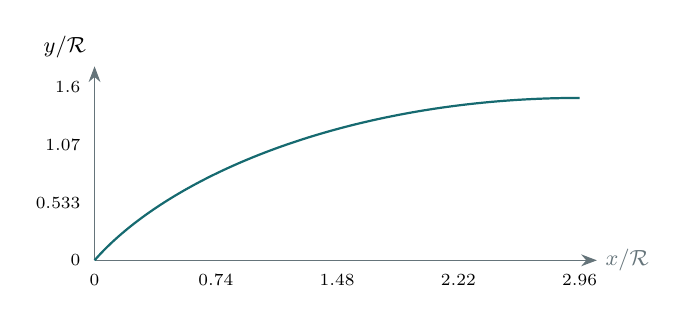
\begin{tikzpicture}[scale=.88,transform shape]
\draw[axis] (0,0.0000000)--(7.25,0.0000000) node[right] {$x/\mathcal R$};
\draw[axis] (0.0000000,0)--(0.0000000,2.8);
\node[above left] at (0.0000000,2.8) {$y/\mathcal R$};
\node[below,font=\scriptsize] at (0.0000000,-0.0800000) {$0$};
\node[below,font=\scriptsize] at (1.7500000,-0.0800000) {$0.74$};
\node[below,font=\scriptsize] at (3.5000000,-0.0800000) {$1.48$};
\node[below,font=\scriptsize] at (5.2500000,-0.0800000) {$2.22$};
\node[below,font=\scriptsize] at (7.0000000,-0.0800000) {$2.96$};
\node[left,font=\scriptsize] at (-0.0800000,0.0000000) {$0$};
\node[left,font=\scriptsize] at (-0.0800000,0.8333333) {$0.533$};
\node[left,font=\scriptsize] at (-0.0800000,1.6666667) {$1.07$};
\node[left,font=\scriptsize] at (-0.0800000,2.5000000) {$1.6$};
\draw[thick,color=accent] plot coordinates {(0.0000000,-0.0000000) (0.0103953,0.0118382) (0.0209473,0.0237350) (0.0316569,0.0356894) (0.0425246,0.0477007) (0.0535514,0.0597678) (0.0647379,0.0718898) (0.0760848,0.0840659) (0.0875929,0.0962951) (0.0992628,0.1085764) (0.1110952,0.1209090) (0.1230909,0.1332918) (0.1352503,0.1457240) (0.1475743,0.1582046) (0.1600635,0.1707326) (0.1727184,0.1833071) (0.1855396,0.1959272) (0.1985278,0.2085918) (0.2116835,0.2213001) (0.2250074,0.2340510) (0.2384999,0.2468435) (0.2521616,0.2596768) (0.2659931,0.2725498) (0.2799948,0.2854615) (0.2941673,0.2984109) (0.3085110,0.3113972) (0.3230265,0.3244192) (0.3377141,0.3374760) (0.3525744,0.3505666) (0.3676079,0.3636900) (0.3828148,0.3768452) (0.3981957,0.3900312) (0.4137509,0.4032470) (0.4294808,0.4164916) (0.4453858,0.4297640) (0.4614662,0.4430631) (0.4777225,0.4563880) (0.4941549,0.4697376) (0.5107637,0.4831109) (0.5275493,0.4965070) (0.5445120,0.5099247) (0.5616520,0.5233631) (0.5789696,0.5368211) (0.5964650,0.5502978) (0.6141386,0.5637920) (0.6319904,0.5773028) (0.6500208,0.5908292) (0.6682299,0.6043700) (0.6866179,0.6179243) (0.7051850,0.6314910) (0.7239313,0.6450692) (0.7428570,0.6586577) (0.7619623,0.6722555) (0.7812471,0.6858617) (0.8007117,0.6994751) (0.8203561,0.7130947) (0.8401804,0.7267195) (0.8601847,0.7403485) (0.8803690,0.7539806) (0.9007333,0.7676148) (0.9212777,0.7812500) (0.9420021,0.7948852) (0.9629066,0.8085194) (0.9839911,0.8221515) (1.0052557,0.8357805) (1.0267002,0.8494053) (1.0483246,0.8630249) (1.0701288,0.8766383) (1.0921128,0.8902445) (1.1142764,0.9038423) (1.1366195,0.9174308) (1.1591420,0.9310090) (1.1818437,0.9445757) (1.2047245,0.9581300) (1.2277842,0.9716708) (1.2510226,0.9851972) (1.2744396,0.9987080) (1.2980349,1.0122022) (1.3218083,1.0256789) (1.3457595,1.0391369) (1.3698883,1.0525753) (1.3941945,1.0659930) (1.4186777,1.0793891) (1.4433376,1.0927624) (1.4681741,1.1061120) (1.4931866,1.1194369) (1.5183750,1.1327360) (1.5437388,1.1460084) (1.5692777,1.1592530) (1.5949913,1.1724688) (1.6208793,1.1856548) (1.6469411,1.1988100) (1.6731765,1.2119334) (1.6995850,1.2250240) (1.7261662,1.2380808) (1.7529195,1.2511028) (1.7798446,1.2640891) (1.8069410,1.2770385) (1.8342081,1.2899502) (1.8616454,1.3028232) (1.8892525,1.3156565) (1.9170288,1.3284490) (1.9449738,1.3411999) (1.9730869,1.3539082) (2.0013675,1.3665728) (2.0298151,1.3791929) (2.0584290,1.3917674) (2.0872087,1.4042954) (2.1161535,1.4167760) (2.1452628,1.4292082) (2.1745360,1.4415910) (2.2039724,1.4539236) (2.2335713,1.4662049) (2.2633320,1.4784341) (2.2932539,1.4906102) (2.3233362,1.5027322) (2.3535783,1.5147993) (2.3839793,1.5268106) (2.4145386,1.5387650) (2.4452554,1.5506618) (2.4761289,1.5625000) (2.5071584,1.5742787) (2.5383430,1.5859970) (2.5696819,1.5976540) (2.6011744,1.6092489) (2.6328196,1.6207806) (2.6646167,1.6322485) (2.6965648,1.6436515) (2.7286630,1.6549889) (2.7609105,1.6662597) (2.7933064,1.6774632) (2.8258498,1.6885984) (2.8585399,1.6996645) (2.8913756,1.7106606) (2.9243560,1.7215860) (2.9574802,1.7324397) (2.9907474,1.7432211) (3.0241564,1.7539291) (3.0577063,1.7645631) (3.0913961,1.7751222) (3.1252250,1.7856056) (3.1591917,1.7960126) (3.1932954,1.8063422) (3.2275350,1.8165938) (3.2619094,1.8267666) (3.2964177,1.8368597) (3.3310587,1.8468724) (3.3658314,1.8568040) (3.4007347,1.8666537) (3.4357676,1.8764207) (3.4709288,1.8861043) (3.5062175,1.8957038) (3.5416323,1.9052184) (3.5771722,1.9146475) (3.6128361,1.9239902) (3.6486227,1.9332458) (3.6845311,1.9424138) (3.7205599,1.9514933) (3.7567080,1.9604837) (3.7929743,1.9693843) (3.8293575,1.9781944) (3.8658564,1.9869134) (3.9024699,1.9955406) (3.9391967,2.0040752) (3.9760356,2.0125168) (4.0129854,2.0208646) (4.0500448,2.0291180) (4.0872125,2.0372763) (4.1244874,2.0453391) (4.1618681,2.0533055) (4.1993534,2.0611751) (4.2369419,2.0689472) (4.2746325,2.0766212) (4.3124237,2.0841966) (4.3503143,2.0916728) (4.3883030,2.0990491) (4.4263885,2.1063252) (4.4645693,2.1135003) (4.5028443,2.1205739) (4.5412120,2.1275456) (4.5796711,2.1344147) (4.6182202,2.1411808) (4.6568580,2.1478433) (4.6955831,2.1544017) (4.7343941,2.1608556) (4.7732896,2.1672044) (4.8122683,2.1734477) (4.8513287,2.1795849) (4.8904695,2.1856157) (4.9296893,2.1915395) (4.9689865,2.1973559) (5.0083598,2.2030645) (5.0478079,2.2086648) (5.0873291,2.2141564) (5.1269222,2.2195388) (5.1665856,2.2248118) (5.2063179,2.2299748) (5.2461177,2.2350274) (5.2859835,2.2399694) (5.3259138,2.2448003) (5.3659072,2.2495197) (5.4059621,2.2541273) (5.4460772,2.2586228) (5.4862509,2.2630057) (5.5264817,2.2672758) (5.5667682,2.2714327) (5.6071088,2.2754762) (5.6475020,2.2794058) (5.6879464,2.2832214) (5.7284405,2.2869226) (5.7689826,2.2905091) (5.8095714,2.2939807) (5.8502053,2.2973371) (5.8908827,2.3005780) (5.9316021,2.3037032) (5.9723621,2.3067125) (6.0131610,2.3096056) (6.0539974,2.3123824) (6.0948696,2.3150425) (6.1357763,2.3175858) (6.1767157,2.3200121) (6.2176864,2.3223213) (6.2586868,2.3245130) (6.2997154,2.3265873) (6.3407706,2.3285439) (6.3818509,2.3303826) (6.4229547,2.3321034) (6.4640804,2.3337060) (6.5052265,2.3351905) (6.5463915,2.3365566) (6.5875736,2.3378042) (6.6287715,2.3389333) (6.6699835,2.3399438) (6.7112081,2.3408356) (6.7524437,2.3416086) (6.7936887,2.3422628) (6.8349415,2.3427982) (6.8762006,2.3432146) (6.9174645,2.3435120) (6.9587314,2.3436905) (7.0000000,2.3437500)};
\end{tikzpicture}
\figcaption{变图综二.3V6\quad 有初速的轨道从摆线拱的内部开始}
\end{minipage}\end{center}
\item \textbf{两层中选择界面交点。}两层厚度均为$1\,\mathrm m$，传播速率分别为$1$和$2\,\mathrm{m/s}$。起点、终点水平相距$2\,\mathrm m$。第一层横向位移为$u$时，
\[
T=\sqrt{1+u^2}+\tfrac12\sqrt{1+(2-u)^2},\quad
T'=\frac{u}{\sqrt{1+u^2}}-\frac{2-u}{2\sqrt{1+(2-u)^2}}
\]
（以米和秒计）。两项来自各层相对竖直方向的正弦除以速率。$T'$严格递增，$T'(0)<0<T'(2)$，故图V7谷底唯一，$u\simeq0.46\,\mathrm m$。较快的第二层承担更多横向路程。
\begin{center}\begin{minipage}{.98\linewidth}\centering
\begin{tikzpicture}[scale=.88,transform shape]
\draw[axis] (0,0.0000000)--(7.25,0.0000000) node[right] {$u/\mathrm{m}$};
\draw[axis] (0.0000000,0)--(0.0000000,2.8);
\node[above left] at (0.0000000,2.8) {$T/\mathrm{s}$};
\node[below,font=\scriptsize] at (0.0000000,-0.0800000) {$0$};
\node[below,font=\scriptsize] at (1.7500000,-0.0800000) {$0.5$};
\node[below,font=\scriptsize] at (3.5000000,-0.0800000) {$1$};
\node[below,font=\scriptsize] at (5.2500000,-0.0800000) {$1.5$};
\node[below,font=\scriptsize] at (7.0000000,-0.0800000) {$2$};
\node[left,font=\scriptsize] at (-0.0800000,0.0000000) {$1.85$};
\node[left,font=\scriptsize] at (-0.0800000,0.8333333) {$2.23$};
\node[left,font=\scriptsize] at (-0.0800000,1.6666667) {$2.62$};
\node[left,font=\scriptsize] at (-0.0800000,2.5000000) {$3$};
\draw[thick,color=accent] plot coordinates {(0.0000000,0.5826826) (0.0291667,0.5746598) (0.0583333,0.5667947) (0.0875000,0.5590874) (0.1166667,0.5515379) (0.1458333,0.5441462) (0.1750000,0.5369121) (0.2041667,0.5298356) (0.2333333,0.5229165) (0.2625000,0.5161548) (0.2916667,0.5095501) (0.3208333,0.5031022) (0.3500000,0.4968111) (0.3791667,0.4906762) (0.4083333,0.4846975) (0.4375000,0.4788744) (0.4666667,0.4732067) (0.4958333,0.4676940) (0.5250000,0.4623358) (0.5541667,0.4571317) (0.5833333,0.4520814) (0.6125000,0.4471842) (0.6416667,0.4424396) (0.6708333,0.4378472) (0.7000000,0.4334063) (0.7291667,0.4291165) (0.7583333,0.4249770) (0.7875000,0.4209873) (0.8166667,0.4171466) (0.8458333,0.4134545) (0.8750000,0.4099101) (0.9041667,0.4065127) (0.9333333,0.4032617) (0.9625000,0.4001563) (0.9916667,0.3971957) (1.0208333,0.3943793) (1.0500000,0.3917061) (1.0791667,0.3891754) (1.1083333,0.3867864) (1.1375000,0.3845383) (1.1666667,0.3824302) (1.1958333,0.3804612) (1.2250000,0.3786306) (1.2541667,0.3769374) (1.2833333,0.3753808) (1.3125000,0.3739599) (1.3416667,0.3726738) (1.3708333,0.3715216) (1.4000000,0.3705023) (1.4291667,0.3696152) (1.4583333,0.3688592) (1.4875000,0.3682334) (1.5166667,0.3677369) (1.5458333,0.3673688) (1.5750000,0.3671281) (1.6041667,0.3670140) (1.6333333,0.3670254) (1.6625000,0.3671615) (1.6916667,0.3674213) (1.7208333,0.3678039) (1.7500000,0.3683083) (1.7791667,0.3689336) (1.8083333,0.3696789) (1.8375000,0.3705432) (1.8666667,0.3715256) (1.8958333,0.3726253) (1.9250000,0.3738412) (1.9541667,0.3751725) (1.9833333,0.3766183) (2.0125000,0.3781776) (2.0416667,0.3798496) (2.0708333,0.3816334) (2.1000000,0.3835281) (2.1291667,0.3855327) (2.1583333,0.3876465) (2.1875000,0.3898686) (2.2166667,0.3921981) (2.2458333,0.3946341) (2.2750000,0.3971759) (2.3041667,0.3998226) (2.3333333,0.4025734) (2.3625000,0.4054274) (2.3916667,0.4083839) (2.4208333,0.4114421) (2.4500000,0.4146012) (2.4791667,0.4178603) (2.5083333,0.4212189) (2.5375000,0.4246760) (2.5666667,0.4282310) (2.5958333,0.4318831) (2.6250000,0.4356316) (2.6541667,0.4394758) (2.6833333,0.4434150) (2.7125000,0.4474485) (2.7416667,0.4515757) (2.7708333,0.4557958) (2.8000000,0.4601083) (2.8291667,0.4645124) (2.8583333,0.4690077) (2.8875000,0.4735933) (2.9166667,0.4782688) (2.9458333,0.4830336) (2.9750000,0.4878870) (3.0041667,0.4928285) (3.0333333,0.4978576) (3.0625000,0.5029737) (3.0916667,0.5081762) (3.1208333,0.5134648) (3.1500000,0.5188388) (3.1791667,0.5242978) (3.2083333,0.5298412) (3.2375000,0.5354687) (3.2666667,0.5411798) (3.2958333,0.5469740) (3.3250000,0.5528509) (3.3541667,0.5588101) (3.3833333,0.5648512) (3.4125000,0.5709738) (3.4416667,0.5771775) (3.4708333,0.5834620) (3.5000000,0.5898268) (3.5291667,0.5962718) (3.5583333,0.6027964) (3.5875000,0.6094005) (3.6166667,0.6160837) (3.6458333,0.6228457) (3.6750000,0.6296863) (3.7041667,0.6366052) (3.7333333,0.6436021) (3.7625000,0.6506768) (3.7916667,0.6578290) (3.8208333,0.6650586) (3.8500000,0.6723654) (3.8791667,0.6797491) (3.9083333,0.6872095) (3.9375000,0.6947466) (3.9666667,0.7023601) (3.9958333,0.7100499) (4.0250000,0.7178159) (4.0541667,0.7256579) (4.0833333,0.7335758) (4.1125000,0.7415696) (4.1416667,0.7496391) (4.1708333,0.7577843) (4.2000000,0.7660051) (4.2291667,0.7743015) (4.2583333,0.7826733) (4.2875000,0.7911207) (4.3166667,0.7996435) (4.3458333,0.8082417) (4.3750000,0.8169153) (4.4041667,0.8256645) (4.4333333,0.8344891) (4.4625000,0.8433891) (4.4916667,0.8523648) (4.5208333,0.8614160) (4.5500000,0.8705429) (4.5791667,0.8797455) (4.6083333,0.8890239) (4.6375000,0.8983782) (4.6666667,0.9078084) (4.6958333,0.9173148) (4.7250000,0.9268974) (4.7541667,0.9365562) (4.7833333,0.9462916) (4.8125000,0.9561036) (4.8416667,0.9659923) (4.8708333,0.9759579) (4.9000000,0.9860005) (4.9291667,0.9961204) (4.9583333,1.0063178) (4.9875000,1.0165927) (5.0166667,1.0269454) (5.0458333,1.0373761) (5.0750000,1.0478850) (5.1041667,1.0584723) (5.1333333,1.0691382) (5.1625000,1.0798830) (5.1916667,1.0907069) (5.2208333,1.1016100) (5.2500000,1.1125927) (5.2791667,1.1236551) (5.3083333,1.1347976) (5.3375000,1.1460204) (5.3666667,1.1573236) (5.3958333,1.1687077) (5.4250000,1.1801728) (5.4541667,1.1917192) (5.4833333,1.2033471) (5.5125000,1.2150569) (5.5416667,1.2268487) (5.5708333,1.2387230) (5.6000000,1.2506798) (5.6291667,1.2627195) (5.6583333,1.2748424) (5.6875000,1.2870487) (5.7166667,1.2993388) (5.7458333,1.3117127) (5.7750000,1.3241710) (5.8041667,1.3367137) (5.8333333,1.3493411) (5.8625000,1.3620536) (5.8916667,1.3748513) (5.9208333,1.3877345) (5.9500000,1.4007035) (5.9791667,1.4137585) (6.0083333,1.4268998) (6.0375000,1.4401275) (6.0666667,1.4534419) (6.0958333,1.4668433) (6.1250000,1.4803318) (6.1541667,1.4939077) (6.1833333,1.5075711) (6.2125000,1.5213223) (6.2416667,1.5351615) (6.2708333,1.5490887) (6.3000000,1.5631043) (6.3291667,1.5772083) (6.3583333,1.5914010) (6.3875000,1.6056824) (6.4166667,1.6200527) (6.4458333,1.6345120) (6.4750000,1.6490604) (6.5041667,1.6636981) (6.5333333,1.6784251) (6.5625000,1.6932415) (6.5916667,1.7081474) (6.6208333,1.7231429) (6.6500000,1.7382279) (6.6791667,1.7534025) (6.7083333,1.7686668) (6.7375000,1.7840207) (6.7666667,1.7994643) (6.7958333,1.8149975) (6.8250000,1.8306202) (6.8541667,1.8463326) (6.8833333,1.8621343) (6.9125000,1.8780256) (6.9416667,1.8940061) (6.9708333,1.9100759) (7.0000000,1.9262347)};
\end{tikzpicture}
\figcaption{变图综二.3V7\quad 两层介质中传播时间随界面交点变化}
\end{minipage}\end{center}
\item \textbf{摆线的法向加速度。}从参数式求曲率半径和法向加速度。令撇号表示对$\varphi$求导，则$x'=\mathcal R(1-\cos\varphi)$、$y'=\mathcal R\sin\varphi$，而$|x'y''-y'x''|=\mathcal R^2(1-\cos\varphi)$。故
\[
\rho=\frac{(x'^2+y'^2)^{3/2}}{|x'y''-y'x''|}=4\mathcal R\sin(\varphi/2),\qquad
a_n=\frac{v^2}{\rho}=g\sin(\varphi/2).
\]
图V8两条曲线均在最低点$\varphi=\pi$处最大，给$\rho=4\mathcal R$和$a_n=g$。切向加速度由$dv/dt=g\cos(\varphi/2)$给出，在最低点恰为零。
\begin{center}\begin{minipage}{.98\linewidth}\centering
\begin{tikzpicture}[scale=.88,transform shape]
\draw[axis] (0,0.0000000)--(7.25,0.0000000) node[right] {$\varphi/\mathrm{rad}$};
\draw[axis] (0.0000000,0)--(0.0000000,2.8);
\node[above left] at (0.0000000,2.8) {$\text{归一化曲率半径与加速度}$};
\node[below,font=\scriptsize] at (0.0000000,-0.0800000) {$0.02$};
\node[below,font=\scriptsize] at (1.7500000,-0.0800000) {$1.58$};
\node[below,font=\scriptsize] at (3.5000000,-0.0800000) {$3.14$};
\node[below,font=\scriptsize] at (5.2500000,-0.0800000) {$4.7$};
\node[below,font=\scriptsize] at (7.0000000,-0.0800000) {$6.26$};
\node[left,font=\scriptsize] at (-0.0800000,0.0000000) {$0$};
\node[left,font=\scriptsize] at (-0.0800000,0.8333333) {$1.4$};
\node[left,font=\scriptsize] at (-0.0800000,1.6666667) {$2.8$};
\node[left,font=\scriptsize] at (-0.0800000,2.5000000) {$4.2$};
\draw[thick,color=accent] plot coordinates {(0.0000000,0.0238091) (0.0291667,0.0547729) (0.0583333,0.0857274) (0.0875000,0.1166673) (0.1166667,0.1475876) (0.1458333,0.1784828) (0.1750000,0.2093479) (0.2041667,0.2401776) (0.2333333,0.2709666) (0.2625000,0.3017098) (0.2916667,0.3324020) (0.3208333,0.3630379) (0.3500000,0.3936124) (0.3791667,0.4241203) (0.4083333,0.4545565) (0.4375000,0.4849158) (0.4666667,0.5151930) (0.4958333,0.5453831) (0.5250000,0.5754809) (0.5541667,0.6054814) (0.5833333,0.6353794) (0.6125000,0.6651699) (0.6416667,0.6948480) (0.6708333,0.7244084) (0.7000000,0.7538464) (0.7291667,0.7831568) (0.7583333,0.8123347) (0.7875000,0.8413752) (0.8166667,0.8702733) (0.8458333,0.8990243) (0.8750000,0.9276231) (0.9041667,0.9560650) (0.9333333,0.9843452) (0.9625000,1.0124588) (0.9916667,1.0404012) (1.0208333,1.0681676) (1.0500000,1.0957533) (1.0791667,1.1231536) (1.1083333,1.1503639) (1.1375000,1.1773796) (1.1666667,1.2041961) (1.1958333,1.2308089) (1.2250000,1.2572135) (1.2541667,1.2834053) (1.2833333,1.3093801) (1.3125000,1.3351334) (1.3416667,1.3606608) (1.3708333,1.3859581) (1.4000000,1.4110208) (1.4291667,1.4358449) (1.4583333,1.4604260) (1.4875000,1.4847601) (1.5166667,1.5088431) (1.5458333,1.5326707) (1.5750000,1.5562391) (1.6041667,1.5795443) (1.6333333,1.6025822) (1.6625000,1.6253490) (1.6916667,1.6478408) (1.7208333,1.6700539) (1.7500000,1.6919844) (1.7791667,1.7136287) (1.8083333,1.7349832) (1.8375000,1.7560441) (1.8666667,1.7768079) (1.8958333,1.7972712) (1.9250000,1.8174304) (1.9541667,1.8372822) (1.9833333,1.8568231) (2.0125000,1.8760500) (2.0416667,1.8949594) (2.0708333,1.9135483) (2.1000000,1.9318135) (2.1291667,1.9497518) (2.1583333,1.9673604) (2.1875000,1.9846361) (2.2166667,2.0015760) (2.2458333,2.0181774) (2.2750000,2.0344373) (2.3041667,2.0503531) (2.3333333,2.0659220) (2.3625000,2.0811415) (2.3916667,2.0960088) (2.4208333,2.1105216) (2.4500000,2.1246773) (2.4791667,2.1384737) (2.5083333,2.1519082) (2.5375000,2.1649787) (2.5666667,2.1776830) (2.5958333,2.1900188) (2.6250000,2.2019842) (2.6541667,2.2135770) (2.6833333,2.2247954) (2.7125000,2.2356374) (2.7416667,2.2461013) (2.7708333,2.2561851) (2.8000000,2.2658873) (2.8291667,2.2752061) (2.8583333,2.2841400) (2.8875000,2.2926876) (2.9166667,2.3008473) (2.9458333,2.3086177) (2.9750000,2.3159976) (3.0041667,2.3229857) (3.0333333,2.3295808) (3.0625000,2.3357819) (3.0916667,2.3415877) (3.1208333,2.3469975) (3.1500000,2.3520102) (3.1791667,2.3566250) (3.2083333,2.3608412) (3.2375000,2.3646579) (3.2666667,2.3680747) (3.2958333,2.3710908) (3.3250000,2.3737058) (3.3541667,2.3759193) (3.3833333,2.3777308) (3.4125000,2.3791400) (3.4416667,2.3801468) (3.4708333,2.3807510) (3.5000000,2.3809524) (3.5291667,2.3807510) (3.5583333,2.3801468) (3.5875000,2.3791400) (3.6166667,2.3777308) (3.6458333,2.3759193) (3.6750000,2.3737058) (3.7041667,2.3710908) (3.7333333,2.3680747) (3.7625000,2.3646579) (3.7916667,2.3608412) (3.8208333,2.3566250) (3.8500000,2.3520102) (3.8791667,2.3469975) (3.9083333,2.3415877) (3.9375000,2.3357819) (3.9666667,2.3295808) (3.9958333,2.3229857) (4.0250000,2.3159976) (4.0541667,2.3086177) (4.0833333,2.3008473) (4.1125000,2.2926876) (4.1416667,2.2841400) (4.1708333,2.2752061) (4.2000000,2.2658873) (4.2291667,2.2561851) (4.2583333,2.2461013) (4.2875000,2.2356374) (4.3166667,2.2247954) (4.3458333,2.2135770) (4.3750000,2.2019842) (4.4041667,2.1900188) (4.4333333,2.1776830) (4.4625000,2.1649787) (4.4916667,2.1519082) (4.5208333,2.1384737) (4.5500000,2.1246773) (4.5791667,2.1105216) (4.6083333,2.0960088) (4.6375000,2.0811415) (4.6666667,2.0659220) (4.6958333,2.0503531) (4.7250000,2.0344373) (4.7541667,2.0181774) (4.7833333,2.0015760) (4.8125000,1.9846361) (4.8416667,1.9673604) (4.8708333,1.9497518) (4.9000000,1.9318135) (4.9291667,1.9135483) (4.9583333,1.8949594) (4.9875000,1.8760500) (5.0166667,1.8568231) (5.0458333,1.8372822) (5.0750000,1.8174304) (5.1041667,1.7972712) (5.1333333,1.7768079) (5.1625000,1.7560441) (5.1916667,1.7349832) (5.2208333,1.7136287) (5.2500000,1.6919844) (5.2791667,1.6700539) (5.3083333,1.6478408) (5.3375000,1.6253490) (5.3666667,1.6025822) (5.3958333,1.5795443) (5.4250000,1.5562391) (5.4541667,1.5326707) (5.4833333,1.5088431) (5.5125000,1.4847601) (5.5416667,1.4604260) (5.5708333,1.4358449) (5.6000000,1.4110208) (5.6291667,1.3859581) (5.6583333,1.3606608) (5.6875000,1.3351334) (5.7166667,1.3093801) (5.7458333,1.2834053) (5.7750000,1.2572135) (5.8041667,1.2308089) (5.8333333,1.2041961) (5.8625000,1.1773796) (5.8916667,1.1503639) (5.9208333,1.1231536) (5.9500000,1.0957533) (5.9791667,1.0681676) (6.0083333,1.0404012) (6.0375000,1.0124588) (6.0666667,0.9843452) (6.0958333,0.9560650) (6.1250000,0.9276231) (6.1541667,0.8990243) (6.1833333,0.8702733) (6.2125000,0.8413752) (6.2416667,0.8123347) (6.2708333,0.7831568) (6.3000000,0.7538464) (6.3291667,0.7244084) (6.3583333,0.6948480) (6.3875000,0.6651699) (6.4166667,0.6353794) (6.4458333,0.6054814) (6.4750000,0.5754809) (6.5041667,0.5453831) (6.5333333,0.5151930) (6.5625000,0.4849158) (6.5916667,0.4545565) (6.6208333,0.4241203) (6.6500000,0.3936124) (6.6791667,0.3630379) (6.7083333,0.3324020) (6.7375000,0.3017098) (6.7666667,0.2709666) (6.7958333,0.2401776) (6.8250000,0.2093479) (6.8541667,0.1784828) (6.8833333,0.1475876) (6.9125000,0.1166673) (6.9416667,0.0857274) (6.9708333,0.0547729) (7.0000000,0.0238091)};
\draw[thick,color=accent] (7.65,2.4)--(8.1,2.4);\node[right,font=\scriptsize] at (8.15,2.4) {$\rho/\mathcal R$};
\draw[thick,dashed,color=warm] plot coordinates {(0.0000000,0.0059523) (0.0291667,0.0136932) (0.0583333,0.0214318) (0.0875000,0.0291668) (0.1166667,0.0368969) (0.1458333,0.0446207) (0.1750000,0.0523370) (0.2041667,0.0600444) (0.2333333,0.0677417) (0.2625000,0.0754275) (0.2916667,0.0831005) (0.3208333,0.0907595) (0.3500000,0.0984031) (0.3791667,0.1060301) (0.4083333,0.1136391) (0.4375000,0.1212289) (0.4666667,0.1287982) (0.4958333,0.1363458) (0.5250000,0.1438702) (0.5541667,0.1513703) (0.5833333,0.1588448) (0.6125000,0.1662925) (0.6416667,0.1737120) (0.6708333,0.1811021) (0.7000000,0.1884616) (0.7291667,0.1957892) (0.7583333,0.2030837) (0.7875000,0.2103438) (0.8166667,0.2175683) (0.8458333,0.2247561) (0.8750000,0.2319058) (0.9041667,0.2390163) (0.9333333,0.2460863) (0.9625000,0.2531147) (0.9916667,0.2601003) (1.0208333,0.2670419) (1.0500000,0.2739383) (1.0791667,0.2807884) (1.1083333,0.2875910) (1.1375000,0.2943449) (1.1666667,0.3010490) (1.1958333,0.3077022) (1.2250000,0.3143034) (1.2541667,0.3208513) (1.2833333,0.3273450) (1.3125000,0.3337834) (1.3416667,0.3401652) (1.3708333,0.3464895) (1.4000000,0.3527552) (1.4291667,0.3589612) (1.4583333,0.3651065) (1.4875000,0.3711900) (1.5166667,0.3772108) (1.5458333,0.3831677) (1.5750000,0.3890598) (1.6041667,0.3948861) (1.6333333,0.4006455) (1.6625000,0.4063372) (1.6916667,0.4119602) (1.7208333,0.4175135) (1.7500000,0.4229961) (1.7791667,0.4284072) (1.8083333,0.4337458) (1.8375000,0.4390110) (1.8666667,0.4442020) (1.8958333,0.4493178) (1.9250000,0.4543576) (1.9541667,0.4593205) (1.9833333,0.4642058) (2.0125000,0.4690125) (2.0416667,0.4737399) (2.0708333,0.4783871) (2.1000000,0.4829534) (2.1291667,0.4874380) (2.1583333,0.4918401) (2.1875000,0.4961590) (2.2166667,0.5003940) (2.2458333,0.5045443) (2.2750000,0.5086093) (2.3041667,0.5125883) (2.3333333,0.5164805) (2.3625000,0.5202854) (2.3916667,0.5240022) (2.4208333,0.5276304) (2.4500000,0.5311693) (2.4791667,0.5346184) (2.5083333,0.5379770) (2.5375000,0.5412447) (2.5666667,0.5444207) (2.5958333,0.5475047) (2.6250000,0.5504960) (2.6541667,0.5533943) (2.6833333,0.5561989) (2.7125000,0.5589094) (2.7416667,0.5615253) (2.7708333,0.5640463) (2.8000000,0.5664718) (2.8291667,0.5688015) (2.8583333,0.5710350) (2.8875000,0.5731719) (2.9166667,0.5752118) (2.9458333,0.5771544) (2.9750000,0.5789994) (3.0041667,0.5807464) (3.0333333,0.5823952) (3.0625000,0.5839455) (3.0916667,0.5853969) (3.1208333,0.5867494) (3.1500000,0.5880025) (3.1791667,0.5891563) (3.2083333,0.5902103) (3.2375000,0.5911645) (3.2666667,0.5920187) (3.2958333,0.5927727) (3.3250000,0.5934265) (3.3541667,0.5939798) (3.3833333,0.5944327) (3.4125000,0.5947850) (3.4416667,0.5950367) (3.4708333,0.5951877) (3.5000000,0.5952381) (3.5291667,0.5951877) (3.5583333,0.5950367) (3.5875000,0.5947850) (3.6166667,0.5944327) (3.6458333,0.5939798) (3.6750000,0.5934265) (3.7041667,0.5927727) (3.7333333,0.5920187) (3.7625000,0.5911645) (3.7916667,0.5902103) (3.8208333,0.5891563) (3.8500000,0.5880025) (3.8791667,0.5867494) (3.9083333,0.5853969) (3.9375000,0.5839455) (3.9666667,0.5823952) (3.9958333,0.5807464) (4.0250000,0.5789994) (4.0541667,0.5771544) (4.0833333,0.5752118) (4.1125000,0.5731719) (4.1416667,0.5710350) (4.1708333,0.5688015) (4.2000000,0.5664718) (4.2291667,0.5640463) (4.2583333,0.5615253) (4.2875000,0.5589094) (4.3166667,0.5561989) (4.3458333,0.5533943) (4.3750000,0.5504960) (4.4041667,0.5475047) (4.4333333,0.5444207) (4.4625000,0.5412447) (4.4916667,0.5379770) (4.5208333,0.5346184) (4.5500000,0.5311693) (4.5791667,0.5276304) (4.6083333,0.5240022) (4.6375000,0.5202854) (4.6666667,0.5164805) (4.6958333,0.5125883) (4.7250000,0.5086093) (4.7541667,0.5045443) (4.7833333,0.5003940) (4.8125000,0.4961590) (4.8416667,0.4918401) (4.8708333,0.4874380) (4.9000000,0.4829534) (4.9291667,0.4783871) (4.9583333,0.4737399) (4.9875000,0.4690125) (5.0166667,0.4642058) (5.0458333,0.4593205) (5.0750000,0.4543576) (5.1041667,0.4493178) (5.1333333,0.4442020) (5.1625000,0.4390110) (5.1916667,0.4337458) (5.2208333,0.4284072) (5.2500000,0.4229961) (5.2791667,0.4175135) (5.3083333,0.4119602) (5.3375000,0.4063372) (5.3666667,0.4006455) (5.3958333,0.3948861) (5.4250000,0.3890598) (5.4541667,0.3831677) (5.4833333,0.3772108) (5.5125000,0.3711900) (5.5416667,0.3651065) (5.5708333,0.3589612) (5.6000000,0.3527552) (5.6291667,0.3464895) (5.6583333,0.3401652) (5.6875000,0.3337834) (5.7166667,0.3273450) (5.7458333,0.3208513) (5.7750000,0.3143034) (5.8041667,0.3077022) (5.8333333,0.3010490) (5.8625000,0.2943449) (5.8916667,0.2875910) (5.9208333,0.2807884) (5.9500000,0.2739383) (5.9791667,0.2670419) (6.0083333,0.2601003) (6.0375000,0.2531147) (6.0666667,0.2460863) (6.0958333,0.2390163) (6.1250000,0.2319058) (6.1541667,0.2247561) (6.1833333,0.2175683) (6.2125000,0.2103438) (6.2416667,0.2030837) (6.2708333,0.1957892) (6.3000000,0.1884616) (6.3291667,0.1811021) (6.3583333,0.1737120) (6.3875000,0.1662925) (6.4166667,0.1588448) (6.4458333,0.1513703) (6.4750000,0.1438702) (6.5041667,0.1363458) (6.5333333,0.1287982) (6.5625000,0.1212289) (6.5916667,0.1136391) (6.6208333,0.1060301) (6.6500000,0.0984031) (6.6791667,0.0907595) (6.7083333,0.0831005) (6.7375000,0.0754275) (6.7666667,0.0677417) (6.7958333,0.0600444) (6.8250000,0.0523370) (6.8541667,0.0446207) (6.8833333,0.0368969) (6.9125000,0.0291668) (6.9416667,0.0214318) (6.9708333,0.0136932) (7.0000000,0.0059523)};
\draw[thick,dashed,color=warm] (7.65,1.9)--(8.1,1.9);\node[right,font=\scriptsize] at (8.15,1.9) {$a_n/g$};
\end{tikzpicture}
\figcaption{变图综二.3V8\quad 摆线的曲率半径和法向加速度沿轨道改变}
\end{minipage}\end{center}
\end{enumerate}

\Needspace{13\baselineskip}

\pdfbookmark[2]{第 4 题 线性引力下的闭合轨道与等效力心}{q4}

\section*{第 4 题\quad 线性引力下的闭合轨道与等效力心}\label{q:4}


设两个质点之间的吸引力与距离一次方成正比，写为
$\boldsymbol F=-GMm\,\boldsymbol r$，其中$\boldsymbol r$从施力质点指向受力质点，$G>0$的量纲按这个假设确定。
\begin{enumerate}
\item 太阳质量$M$固定，忽略行星对太阳的反作用。仿照轨道形状、面积规律和周期规律，建立这种引力下的三条行星运动定律。讨论轨道所在平面、椭圆力心位置及退化情况。
\item 若施力者为固定在$\boldsymbol R_i$处的若干质量$M_i>0$的质点，求受力质点一般轨道，说明能否用一个等效力心统一描述。
\end{enumerate}
讨论轨道时排除受力物体与实体施力物体相撞的情形。


\begin{center}\begin{minipage}{.98\linewidth}\centering
\begin{tikzpicture}[scale=.8,transform shape]

\draw[axis] (-.5,0)--(4.4,0) node[right] {$x$};
\draw[axis] (0,-.5)--(0,3.3) node[above] {$y$};
\fill (0,0) circle (2pt) node[below left] {$M$};
\fill (2.5,1.5) circle (2pt) node[right] {$m$};
\draw[guide] (0,0)--(2.5,1.5) node[midway,above left] {$\boldsymbol r$};
\draw[force] (2.5,1.5)--(1.25,.75) node[midway,below right] {$\boldsymbol F$};
\draw[motion] (2.5,1.5)--(3,3) node[above] {$\boldsymbol v$};
\begin{scope}[xshift=7cm]
\fill (-1,0) circle (2pt) node[left] {$M_1$};
\fill (1.5,1.8) circle (3pt) node[above] {$M_2$};
\fill (1.3,-1) circle (2pt) node[below] {$M_3$};
\fill (3,.4) circle (2pt) node[right] {$m$};
\draw[guide] (-1,0)--(3,.4); \draw[guide] (1.5,1.8)--(3,.4); \draw[guide] (1.3,-1)--(3,.4);
\end{scope}

\end{tikzpicture}
\figcaption{图综二.4\quad 单个线性中心力与任意固定源组，两种情形分别求轨道。}
\end{minipage}\end{center}

\Needspace{8\baselineskip}

\pdfbookmark[3]{题型定位}{q4-h0}

\subsection*{题型定位}

通过各方向同频谐振建立线性中心力的闭合轨道规律，对固定源组直接收集位置矢量项，求出总质量和等效中心。

\Needspace{8\baselineskip}

\pdfbookmark[3]{知识点}{q4-h1}

\subsection*{知识点}

\begin{itemize}
\item 线性中心力、矢量简谐振动显式解。
\item 轨道平面、同频振动合成椭圆和相位退化。
\item 角动量、面积速度和尺寸无关的公转周期。
\item 固定质量组质心、平方和分解及等效力心。
\end{itemize}

\Needspace{8\baselineskip}

\pdfbookmark[3]{物理图像}{q4-h2}

\subsection*{物理图像}

图A用两初矢量的线性组合构成椭圆，太阳在中心。图B中$\boldsymbol R_C$以质量加权，三个固定源的作用叠加成指向$C$的合力。图C把合力对应到等势圆和二次势能。图D的等质量源则说明，只有距离系数恒定时，任意质点组都能按同一质量权重合并。

\Needspace{8\baselineskip}

\pdfbookmark[3]{解题入口}{q4-h3}

\subsection*{解题入口}

先把题给的引力大小乘指向太阳的单位矢量，使距离因子变成位置矢量。解三个同频分量，$z=\dot z=0$的初值给平面内运动，两个面内初值构成椭圆。再从力矩和共同频率分别求面积速度与周期。多源时，用图B把每一根位移写成$\boldsymbol r-\boldsymbol R_i$，提取共同的$\boldsymbol r$，剩下的固定项给出质心。

\Needspace{8\baselineskip}

\pdfbookmark[3]{标准解法}{q4-h4}

\subsection*{标准解法}


题设的力大小为$GMmr$，其中$G$的单位由力式确定为$\mathrm{kg^{-1}s^{-2}}$。将力的大小乘以朝向太阳的单位矢量，距离$r$便和单位矢量的分母约去，留下$-GMm\boldsymbol r$。这一步决定了分运动的形式。若$\boldsymbol r$与$x$轴夹角为$\theta$，则$F_x=-GMmr\cos\theta=-GMmx$、$F_y=-GMmr\sin\theta=-GMmy$。两个方向各有一条线性恢复力，弹性系数都为$GMm$，所以它们共有一个角频率。

图综二.4中力始终指向太阳。运动方程为
\[
\ddot{\boldsymbol r}=-GM\,\boldsymbol r=-\omega^2\boldsymbol r,
\qquad \omega=\sqrt{GM}.
\]
给定初位置$\boldsymbol r_0$和初速度$\boldsymbol v_0$，矢量解为
\[
\boxed{\boldsymbol r(t)=\boldsymbol r_0\cos\omega t+
\frac{\boldsymbol v_0}{\omega}\sin\omega t}.
\]
两个初矢量线性独立时，任意时刻的位置都在它们张成的平面内。只有一个独立方向时，运动退化为沿这条直线往复。两初矢量均为零时，质点静止在太阳所在的力心。
取$Oxy$为$\boldsymbol r_0,\boldsymbol v_0$张成的平面，则初始$z=\dot z=0$，且$\ddot z=-GMz$。这个一维初值问题的解恒为零，说明从平面内出发就留在平面内。对一般有心力，$\boldsymbol r\times\boldsymbol F=0$给固定的角动量方向，非零角动量同样确定运动平面。初始矢量共线时，沿该直线取一条坐标轴，其余两个坐标的初值与速度均为零，于是只剩轴上的振动。

\begin{center}\begin{minipage}{.98\linewidth}\centering
\begin{tikzpicture}[scale=.85,transform shape]

\draw[object] (0,0) ellipse (3 and 1.5);
\fill (0,0) circle (2pt) node[below left] {$O$太阳};
\draw[guide] (0,0)--(3,0) node[midway,below] {$\boldsymbol r_0$};
\draw[motion] (3,0)--(3,2) node[above] {$\boldsymbol v_0$};
\draw[force] (3,0)--(1.7,0) node[midway,above] {$\boldsymbol F$};
\node at (0,2.6) {图示为两初矢量正交的主轴坐标};
\node at (0,-2.7) {$\boldsymbol r(t)=\boldsymbol r_0\cos\omega t+
(\boldsymbol v_0/\omega)\sin\omega t$};

\end{tikzpicture}
\figcaption{解图综二.4A\quad 同频振动合成中心椭圆，力心在椭圆中心。}
\end{minipage}\end{center}
解图综二.4A把两个初矢量作为构造椭圆的两个系数。在平面直角坐标下，也可写为
\[
x=A\cos(\omega t+\phi_1),\qquad
y=B\cos(\omega t+\phi_2).
\]
振幅和相位可从初值直接读出。例如$x(0)=A\cos\phi_1$、$\dot x(0)=-A\omega\sin\phi_1$，所以$A^2=x(0)^2+[\dot x(0)/\omega]^2$，两式分别确定相位的余弦和正弦。$y$方向同理。令$u=\omega t+\phi_1$、$\delta=\phi_2-\phi_1$，则$x/A=\cos u$、$y/B=\cos u\cos\delta-\sin u\sin\delta$。把后一式移项后平方，再用$\sin^2u=1-\cos^2u$，就得到轨道方程。若某一振幅为零，轨道已在另一条轴上。

取两个振幅均为正的情形，消去$t$得到
\[
\boxed{\frac{x^2}{A^2}+\frac{y^2}{B^2}
-\frac{2xy}{AB}\cos(\phi_2-\phi_1)
=\sin^2(\phi_2-\phi_1)}.
\]
这个椭圆还可从初值直接求出长、短半轴。取一个以太阳为原点的平面直角坐标，把$\boldsymbol r_0$和$\boldsymbol v_0/\omega$作为两列组成矩阵$K$。若这两列不共线，则$x,y$的二次式写为$\boldsymbol r^{\mathsf T}(KK^{\mathsf T})^{-1}\boldsymbol r=1$。$KK^{\mathsf T}$的两个正特征值就是$a^2,b^2$，对应的单位特征矢量给主轴方向。这些值的和、积分别是
\[
a^2+b^2=|\boldsymbol r_0|^2+|\boldsymbol v_0|^2/\omega^2,\qquad
a^2b^2=|\boldsymbol r_0\times\boldsymbol v_0|^2/\omega^2.
\]
前一式说明能量决定两个半轴平方的和，后一式说明角动量决定椭圆的面积。给定初位置和初速度即可分别算出两半轴。若两个特征值相等，力心到轨道各点的距离相同，椭圆化为圆。若其中一个为零，线性变换把单位圆压在一条直线上，往、返两程各走同一个线段。

当$\phi_2-\phi_1$不是$\pi$的整数倍时，这是中心位于太阳的椭圆；旋转坐标可化为无交叉项的长短轴形式，圆为特殊情形。若相位差为$\pi$的整数倍，椭圆退化为直线段。点力模型中的质点沿直线穿过中心。有有限半径的太阳占据中心附近空间，此直线轨迹会碰到太阳。

由此第一条规律为：\textbf{非退化行星轨道为椭圆，太阳在各椭圆共同中心。}


中心力力矩为零：
\[
\frac d{dt}\left(m\boldsymbol r\times\dot{\boldsymbol r}\right)
=\boldsymbol r\times\boldsymbol F=0.
\]
第二条规律仍为：\textbf{太阳到行星的连线在相等时间扫过相等面积。}
面积速度是
\[
\dot{\mathcal A}
=\frac12|\boldsymbol r\times\dot{\boldsymbol r}|
=\frac{|\boldsymbol L|}{2m}.
\]
对主轴为$a,b$的参数解$x=a\cos\omega t,y=b\sin\omega t$，它还等于$ab\omega/2$，一周面积$\pi ab$。椭圆的极角速度由$\dot\theta=L_z/(mr^2)$给出。短轴端离太阳近，单位时间转过的极角大，长轴端则较小。振动相位的变化率$\omega$恒定，极角的变化率随矢径长度改变。

非共线时两个初矢量线性独立。图A的参数关系可看作将单位圆坐标$(\cos\omega t,\sin\omega t)$沿两个初矢量作线性变换，得到有面积的椭圆。半周期后位置变为$-\boldsymbol r$，正好走到椭圆的另一端。回到同一位置要求两个系数都回到初值，故最短公转周期等于两个分运动的共同周期。逐一对应开普勒三定律时，第一条改变了太阳在椭圆中的位置，第二条由中心力性质保留，第三条由角频率仅含$GM$得出同一太阳下的周期相等。

两个分运动频率相同，非退化轨道的最小公转周期是
\[
\boxed{T=\frac{2\pi}{\sqrt{GM}}}.
\]
所以第三条规律为：\textbf{围绕同一固定太阳的所有行星周期相同，与椭圆的大小、长短轴比以及行星质量无关。}

\begin{center}\begin{minipage}{.98\linewidth}\centering
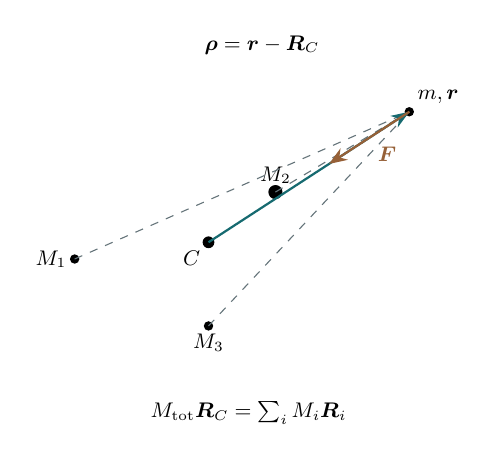
\begin{tikzpicture}[scale=.85,transform shape]

\fill (-1,0) circle (2pt) node[left] {$M_1$};
\fill (2,1) circle (3pt) node[above] {$M_2$};
\fill (1,-1) circle (2pt) node[below] {$M_3$};
\coordinate (C) at (1,.25); \fill (C) circle (2.5pt) node[below left] {$C$};
\coordinate (P) at (4,2.2); \fill (P) circle (2pt) node[above right] {$m,\boldsymbol r$};
\draw[guide] (-1,0)--(P); \draw[guide] (2,1)--(P); \draw[guide] (1,-1)--(P);
\draw[motion] (C)--(P);
\node at (1.8,3.2) {$\boldsymbol\rho=\boldsymbol r-\boldsymbol R_C$};
\draw[force] (P)--(2.8,1.42) node[midway,below right] {$\boldsymbol F$};
\node at (1.6,-2.3) {$M_{\rm tot}\boldsymbol R_C=\sum_iM_i\boldsymbol R_i$};

\end{tikzpicture}
\figcaption{解图综二.4B\quad 线性位置项求和后等效于总质量集中在固定质心。}
\end{minipage}\end{center}
第（2）问，解图综二.4B以任意固定原点表示源组位置。对受力点$\boldsymbol r$，
\[
\begin{aligned}
\boldsymbol F
&=-Gm\sum_iM_i(\boldsymbol r-\boldsymbol R_i)\\
&=-Gm\left[\left(\sum_iM_i\right)\boldsymbol r
-\sum_iM_i\boldsymbol R_i\right].
\end{aligned}
\]
定义源组总质量和质心
\[
M_{\rm tot}=\sum_iM_i,\qquad
\boldsymbol R_C=\frac{\sum_iM_i\boldsymbol R_i}{M_{\rm tot}},
\]
则
\[
\boxed{\boldsymbol F=-GmM_{\rm tot}(\boldsymbol r-\boldsymbol R_C)}.
\]
这个合力式在任意受力点成立，图B的三个源可以有任意空间分布。以$\boldsymbol \rho=\boldsymbol r-\boldsymbol R_C$为相对位置，
\[
\ddot{\boldsymbol \rho}+GM_{\rm tot}\boldsymbol\rho=0.
\]
把图B各虚线的方向统一为从$M_i$指向受力点。因作用力与这根矢量成正比，各项的受力点坐标都是同一个$\boldsymbol r$，可提出求和号。图示取$M_2=2M_1=2M_3$，所以$C$向$M_2$一侧偏移。把坐标原点移至$C$，新的初位置用$\boldsymbol r_0-\boldsymbol R_C$，初速度照旧。只要轨道与各固定质点在空间上分开，图A关于中心、面积和周期的结论便可逐一用于这组力。初相对位置与初速度共线且至少一个非零时，质点沿这条线往复。若初相对位置与速度都为零，它静止在$C$。

因此一般为以固定质心$C$为中心的平面椭圆，周期
$2\pi/\sqrt{GM_{\rm tot}}$；初相对位置与初速度共线时仍退化为直线段。
\begin{center}\begin{minipage}{.98\linewidth}\centering
\begin{tikzpicture}[scale=.8,transform shape]

\draw[guide] (0,0) circle (1); \draw[guide] (0,0) circle (2);
\draw[object] (0,0) ellipse (2.5 and 1.2);
\fill (0,0) circle (2pt) node[below left] {$C$};
\node at (0,3) {相对质心的等势圆与轨道};
\begin{scope}[xshift=6cm]
\draw[axis] (-2.3,0)--(2.3,0) node[right] {$s$};
\draw[axis] (0,-.3)--(0,3) node[above] {$U-U_0$};
\draw[traj,domain=-2:2,samples=100] plot (\x,{.6*\x*\x});
\node at (0,-1.4) {$U-U_0=GmM_{\rm tot}s^2/2$};
\end{scope}

\end{tikzpicture}
\figcaption{解图综二.4C\quad 源组位置只给势能增添常量，受力点的势能仍为各向同性二次型。}
\end{minipage}\end{center}
解图综二.4C用势能的负梯度$\boldsymbol F=-\nabla U$表示上述合力。
\[
\begin{aligned}
U&=\frac{Gm}{2}\sum_iM_i|\boldsymbol r-\boldsymbol R_i|^2\\
&=\frac{GmM_{\rm tot}}2|\boldsymbol r-\boldsymbol R_C|^2
+\frac{Gm}{2}\sum_iM_i|\boldsymbol R_i-\boldsymbol R_C|^2 .
\end{aligned}
\]
第二项不随受力点改变，只是势能零点的常量；第一项给出同一线性中心力。沿经过$C$的一条直径取有符号坐标$s$，图C的右半幅画的是这条直径上关于$s$的抛物线。
这种集中到质心的规律对源的位置没有对称性要求。通常的平方反比引力和库仑力则给每根位移矢量乘上各自距离的负三次方，系数随受力点移动而变化。球对称分布在球外可集中到球心，因为球对称使场在每个同心球面上等强，再由通量求出径向场。对于任意离散源组，各距离的权重需逐项保留。

解图综二.4D用最简单的两个等质量源说明，若要求任意源组都能集中到质心，力的径向大小为什么与距离成正比。设距离为$\ell$时的力写成$-GmM c(\ell)\boldsymbol\ell$。两个源各在$C$的左右$d$处，受力点$P$在垂直平分线上，离$C$为$s>0$。图D的两个水平分量互相抵消，竖直合力为$-2GmM s c(\sqrt{s^2+d^2})$。若等效为质心处总质量$2M$，竖直合力应为$-2GmM s c(s)$。比较得
\[
c(\sqrt{s^2+d^2})=c(s)\qquad(s>0,\ d>0).
\]
改变$d$可让左边的自变量取大于$s$的任意距离，故$c$在正半轴上为常量。线性力正满足这一关系，因而任意固定源组都可如此合并。
\begin{center}\begin{minipage}{.98\linewidth}\centering
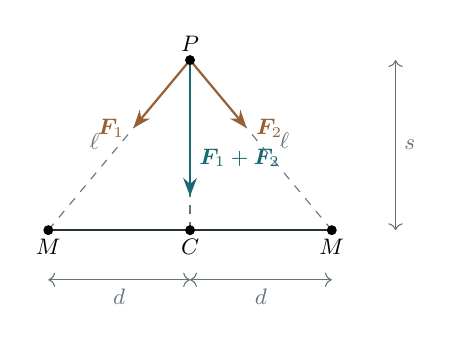
\begin{tikzpicture}[scale=.9,transform shape]
\coordinate (L) at (-2,0); \coordinate (C) at (0,0); \coordinate (R) at (2,0); \coordinate (P) at (0,2.4);
\draw[guide] (L)--(P) node[pos=.42,above left] {$\ell$};
\draw[guide] (R)--(P) node[pos=.43,above right] {$\ell$};
\draw[object] (L)--(R);
\draw[guide] (C)--(P);
\draw[force] (P)--(-.8,1.44) node[left] {$\boldsymbol F_1$};
\draw[force] (P)--(.8,1.44) node[right] {$\boldsymbol F_2$};
\draw[motion] (P)--(0,.48) node[pos=.72,right] {$\boldsymbol F_1+\boldsymbol F_2$};
\draw[axis,<->] (2.9,0)--(2.9,2.4) node[midway,right] {$s$};
\fill (L) circle (2pt) node[below] {$M$}; \fill (R) circle (2pt) node[below] {$M$};
\fill (C) circle (2pt) node[below] {$C$}; \fill (P) circle (2pt) node[above] {$P$};
\draw[axis,<->] (-2,-.7)--(0,-.7) node[midway,below] {$d$};
\draw[axis,<->] (0,-.7)--(2,-.7) node[midway,below] {$d$};
\end{tikzpicture}
\figcaption{解图综二.4D\quad 两个等质量源的合力沿垂直平分线。}
\end{minipage}\end{center}



\Needspace{8\baselineskip}

\pdfbookmark[3]{关键洞察}{q4-h5}

\subsection*{关键洞察}

各向同性线性恢复力使两个分运动同频，因而椭圆在同一周期后闭合。多源叠加时，各项系数是固定的$GM_i$，提取受力点的位置后，剩下的固定矢量给质量加权的中心。图D从垂直平分线上的力分量说明这个条件的必要性。

\Needspace{8\baselineskip}

\pdfbookmark[3]{易错点}{q4-h6}

\subsection*{易错点}

\begin{itemize}
\item 把线性力的G误认为通常平方反比引力常量而混用量纲。
\item 椭圆算出后仍把太阳放在焦点。
\item 忽略两个分运动同频，套用一般不同频率李萨如曲线。
\item 将角动量零的直线退化当成不撞太阳的公转。
\item 只把源质量相加却不移动到质量加权质心，或对平方反比源组照搬约化。
\end{itemize}

\Needspace{8\baselineskip}

\pdfbookmark[3]{课堂讲解建议}{q4-h7}

\subsection*{课堂讲解建议}

在图A问“为什么$z$一直为零？”学生写出$\ddot z=-GMz$及零初值，再用唯一解说明运动留在平面内。接着让学生把$\omega t$加上$\pi$，用两个分量的符号反转指出轨道的另一端。比较三条轨道规律时，要求分别说出中心位置、面积速度、周期所由来的方程。图B改成质量为$M$和$3M$的两个源，问“合力零点在两源中点吗？”由图V2的直线零点得到$3d/4$。再将图D的$P$上移，追问平方反比力的两项权重如何变化，学生可直接用$s$和$\sqrt{s^2+d^2}$比较。

\Needspace{8\baselineskip}

\pdfbookmark[3]{变式训练}{q4-h8}

\subsection*{变式训练}

\begin{enumerate}
\item \textbf{两个等质量源移远。}在$x=\pm d$固定两个质量$M$，求受力点的合力与周期，再把源移到$\pm2d$。质心都在$O$，合力为$-2GMm\boldsymbol r$，周期为$2\pi/\sqrt{2GM}$。沿$x$轴，令$X=x/d$，则
\[
\frac{U_d}{GMmd^2}=X^2+1,\qquad
\frac{U_{2d}}{GMmd^2}=X^2+4.
\]
图V1两条势能曲线的差为常量3，在同一点的斜率相同，所以力与周期保持相同。把质点移到轴外也只改变共同的$|\boldsymbol r|^2$项。
\begin{center}\begin{minipage}{.98\linewidth}\centering
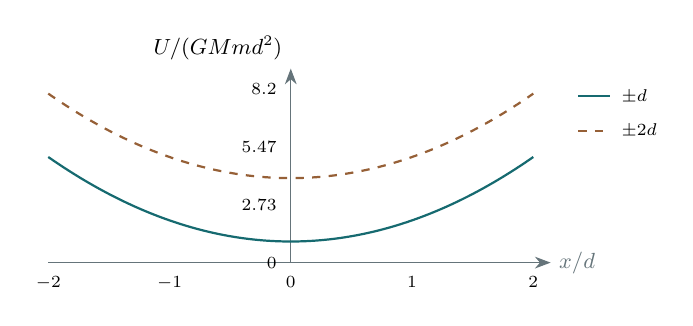
\begin{tikzpicture}[scale=.88,transform shape]
\draw[axis] (0,0.0000000)--(7.25,0.0000000) node[right] {$x/d$};
\draw[axis] (3.5000000,0)--(3.5000000,2.8);
\node[above left] at (3.5000000,2.8) {$U/(GMmd^2)$};
\node[below,font=\scriptsize] at (0.0000000,-0.0800000) {$-2$};
\node[below,font=\scriptsize] at (1.7500000,-0.0800000) {$-1$};
\node[below,font=\scriptsize] at (3.5000000,-0.0800000) {$0$};
\node[below,font=\scriptsize] at (5.2500000,-0.0800000) {$1$};
\node[below,font=\scriptsize] at (7.0000000,-0.0800000) {$2$};
\node[left,font=\scriptsize] at (3.4200000,0.0000000) {$0$};
\node[left,font=\scriptsize] at (3.4200000,0.8333333) {$2.73$};
\node[left,font=\scriptsize] at (3.4200000,1.6666667) {$5.47$};
\node[left,font=\scriptsize] at (3.4200000,2.5000000) {$8.2$};
\draw[thick,color=accent] plot coordinates {(0.0000000,1.5243902) (0.0291667,1.5041497) (0.0583333,1.4840786) (0.0875000,1.4641768) (0.1166667,1.4444444) (0.1458333,1.4248814) (0.1750000,1.4054878) (0.2041667,1.3862636) (0.2333333,1.3672087) (0.2625000,1.3483232) (0.2916667,1.3296070) (0.3208333,1.3110603) (0.3500000,1.2926829) (0.3791667,1.2744749) (0.4083333,1.2564363) (0.4375000,1.2385671) (0.4666667,1.2208672) (0.4958333,1.2033367) (0.5250000,1.1859756) (0.5541667,1.1687839) (0.5833333,1.1517615) (0.6125000,1.1349085) (0.6416667,1.1182249) (0.6708333,1.1017107) (0.7000000,1.0853659) (0.7291667,1.0691904) (0.7583333,1.0531843) (0.7875000,1.0373476) (0.8166667,1.0216802) (0.8458333,1.0061822) (0.8750000,0.9908537) (0.9041667,0.9756944) (0.9333333,0.9607046) (0.9625000,0.9458841) (0.9916667,0.9312331) (1.0208333,0.9167514) (1.0500000,0.9024390) (1.0791667,0.8882961) (1.1083333,0.8743225) (1.1375000,0.8605183) (1.1666667,0.8468835) (1.1958333,0.8334180) (1.2250000,0.8201220) (1.2541667,0.8069953) (1.2833333,0.7940379) (1.3125000,0.7812500) (1.3416667,0.7686314) (1.3708333,0.7561822) (1.4000000,0.7439024) (1.4291667,0.7317920) (1.4583333,0.7198509) (1.4875000,0.7080793) (1.5166667,0.6964770) (1.5458333,0.6850440) (1.5750000,0.6737805) (1.6041667,0.6626863) (1.6333333,0.6517615) (1.6625000,0.6410061) (1.6916667,0.6304201) (1.7208333,0.6200034) (1.7500000,0.6097561) (1.7791667,0.5996782) (1.8083333,0.5897696) (1.8375000,0.5800305) (1.8666667,0.5704607) (1.8958333,0.5610603) (1.9250000,0.5518293) (1.9541667,0.5427676) (1.9833333,0.5338753) (2.0125000,0.5251524) (2.0416667,0.5165989) (2.0708333,0.5082148) (2.1000000,0.5000000) (2.1291667,0.4919546) (2.1583333,0.4840786) (2.1875000,0.4763720) (2.2166667,0.4688347) (2.2458333,0.4614668) (2.2750000,0.4542683) (2.3041667,0.4472392) (2.3333333,0.4403794) (2.3625000,0.4336890) (2.3916667,0.4271680) (2.4208333,0.4208164) (2.4500000,0.4146341) (2.4791667,0.4086213) (2.5083333,0.4027778) (2.5375000,0.3971037) (2.5666667,0.3915989) (2.5958333,0.3862636) (2.6250000,0.3810976) (2.6541667,0.3761009) (2.6833333,0.3712737) (2.7125000,0.3666159) (2.7416667,0.3621274) (2.7708333,0.3578083) (2.8000000,0.3536585) (2.8291667,0.3496782) (2.8583333,0.3458672) (2.8875000,0.3422256) (2.9166667,0.3387534) (2.9458333,0.3354505) (2.9750000,0.3323171) (3.0041667,0.3293530) (3.0333333,0.3265583) (3.0625000,0.3239329) (3.0916667,0.3214770) (3.1208333,0.3191904) (3.1500000,0.3170732) (3.1791667,0.3151253) (3.2083333,0.3133469) (3.2375000,0.3117378) (3.2666667,0.3102981) (3.2958333,0.3090278) (3.3250000,0.3079268) (3.3541667,0.3069953) (3.3833333,0.3062331) (3.4125000,0.3056402) (3.4416667,0.3052168) (3.4708333,0.3049627) (3.5000000,0.3048780) (3.5291667,0.3049627) (3.5583333,0.3052168) (3.5875000,0.3056402) (3.6166667,0.3062331) (3.6458333,0.3069953) (3.6750000,0.3079268) (3.7041667,0.3090278) (3.7333333,0.3102981) (3.7625000,0.3117378) (3.7916667,0.3133469) (3.8208333,0.3151253) (3.8500000,0.3170732) (3.8791667,0.3191904) (3.9083333,0.3214770) (3.9375000,0.3239329) (3.9666667,0.3265583) (3.9958333,0.3293530) (4.0250000,0.3323171) (4.0541667,0.3354505) (4.0833333,0.3387534) (4.1125000,0.3422256) (4.1416667,0.3458672) (4.1708333,0.3496782) (4.2000000,0.3536585) (4.2291667,0.3578083) (4.2583333,0.3621274) (4.2875000,0.3666159) (4.3166667,0.3712737) (4.3458333,0.3761009) (4.3750000,0.3810976) (4.4041667,0.3862636) (4.4333333,0.3915989) (4.4625000,0.3971037) (4.4916667,0.4027778) (4.5208333,0.4086213) (4.5500000,0.4146341) (4.5791667,0.4208164) (4.6083333,0.4271680) (4.6375000,0.4336890) (4.6666667,0.4403794) (4.6958333,0.4472392) (4.7250000,0.4542683) (4.7541667,0.4614668) (4.7833333,0.4688347) (4.8125000,0.4763720) (4.8416667,0.4840786) (4.8708333,0.4919546) (4.9000000,0.5000000) (4.9291667,0.5082148) (4.9583333,0.5165989) (4.9875000,0.5251524) (5.0166667,0.5338753) (5.0458333,0.5427676) (5.0750000,0.5518293) (5.1041667,0.5610603) (5.1333333,0.5704607) (5.1625000,0.5800305) (5.1916667,0.5897696) (5.2208333,0.5996782) (5.2500000,0.6097561) (5.2791667,0.6200034) (5.3083333,0.6304201) (5.3375000,0.6410061) (5.3666667,0.6517615) (5.3958333,0.6626863) (5.4250000,0.6737805) (5.4541667,0.6850440) (5.4833333,0.6964770) (5.5125000,0.7080793) (5.5416667,0.7198509) (5.5708333,0.7317920) (5.6000000,0.7439024) (5.6291667,0.7561822) (5.6583333,0.7686314) (5.6875000,0.7812500) (5.7166667,0.7940379) (5.7458333,0.8069953) (5.7750000,0.8201220) (5.8041667,0.8334180) (5.8333333,0.8468835) (5.8625000,0.8605183) (5.8916667,0.8743225) (5.9208333,0.8882961) (5.9500000,0.9024390) (5.9791667,0.9167514) (6.0083333,0.9312331) (6.0375000,0.9458841) (6.0666667,0.9607046) (6.0958333,0.9756944) (6.1250000,0.9908537) (6.1541667,1.0061822) (6.1833333,1.0216802) (6.2125000,1.0373476) (6.2416667,1.0531843) (6.2708333,1.0691904) (6.3000000,1.0853659) (6.3291667,1.1017107) (6.3583333,1.1182249) (6.3875000,1.1349085) (6.4166667,1.1517615) (6.4458333,1.1687839) (6.4750000,1.1859756) (6.5041667,1.2033367) (6.5333333,1.2208672) (6.5625000,1.2385671) (6.5916667,1.2564363) (6.6208333,1.2744749) (6.6500000,1.2926829) (6.6791667,1.3110603) (6.7083333,1.3296070) (6.7375000,1.3483232) (6.7666667,1.3672087) (6.7958333,1.3862636) (6.8250000,1.4054878) (6.8541667,1.4248814) (6.8833333,1.4444444) (6.9125000,1.4641768) (6.9416667,1.4840786) (6.9708333,1.5041497) (7.0000000,1.5243902)};
\draw[thick,color=accent] (7.65,2.4)--(8.1,2.4);\node[right,font=\scriptsize] at (8.15,2.4) {$\pm d$};
\draw[thick,dashed,color=warm] plot coordinates {(0.0000000,2.4390244) (0.0291667,2.4187839) (0.0583333,2.3987127) (0.0875000,2.3788110) (0.1166667,2.3590786) (0.1458333,2.3395156) (0.1750000,2.3201220) (0.2041667,2.3008977) (0.2333333,2.2818428) (0.2625000,2.2629573) (0.2916667,2.2442412) (0.3208333,2.2256944) (0.3500000,2.2073171) (0.3791667,2.1891091) (0.4083333,2.1710705) (0.4375000,2.1532012) (0.4666667,2.1355014) (0.4958333,2.1179709) (0.5250000,2.1006098) (0.5541667,2.0834180) (0.5833333,2.0663957) (0.6125000,2.0495427) (0.6416667,2.0328591) (0.6708333,2.0163449) (0.7000000,2.0000000) (0.7291667,1.9838245) (0.7583333,1.9678184) (0.7875000,1.9519817) (0.8166667,1.9363144) (0.8458333,1.9208164) (0.8750000,1.9054878) (0.9041667,1.8903286) (0.9333333,1.8753388) (0.9625000,1.8605183) (0.9916667,1.8458672) (1.0208333,1.8313855) (1.0500000,1.8170732) (1.0791667,1.8029302) (1.1083333,1.7889566) (1.1375000,1.7751524) (1.1666667,1.7615176) (1.1958333,1.7480522) (1.2250000,1.7347561) (1.2541667,1.7216294) (1.2833333,1.7086721) (1.3125000,1.6958841) (1.3416667,1.6832656) (1.3708333,1.6708164) (1.4000000,1.6585366) (1.4291667,1.6464262) (1.4583333,1.6344851) (1.4875000,1.6227134) (1.5166667,1.6111111) (1.5458333,1.5996782) (1.5750000,1.5884146) (1.6041667,1.5773205) (1.6333333,1.5663957) (1.6625000,1.5556402) (1.6916667,1.5450542) (1.7208333,1.5346375) (1.7500000,1.5243902) (1.7791667,1.5143123) (1.8083333,1.5044038) (1.8375000,1.4946646) (1.8666667,1.4850949) (1.8958333,1.4756944) (1.9250000,1.4664634) (1.9541667,1.4574018) (1.9833333,1.4485095) (2.0125000,1.4397866) (2.0416667,1.4312331) (2.0708333,1.4228489) (2.1000000,1.4146341) (2.1291667,1.4065888) (2.1583333,1.3987127) (2.1875000,1.3910061) (2.2166667,1.3834688) (2.2458333,1.3761009) (2.2750000,1.3689024) (2.3041667,1.3618733) (2.3333333,1.3550136) (2.3625000,1.3483232) (2.3916667,1.3418022) (2.4208333,1.3354505) (2.4500000,1.3292683) (2.4791667,1.3232554) (2.5083333,1.3174119) (2.5375000,1.3117378) (2.5666667,1.3062331) (2.5958333,1.3008977) (2.6250000,1.2957317) (2.6541667,1.2907351) (2.6833333,1.2859079) (2.7125000,1.2812500) (2.7416667,1.2767615) (2.7708333,1.2724424) (2.8000000,1.2682927) (2.8291667,1.2643123) (2.8583333,1.2605014) (2.8875000,1.2568598) (2.9166667,1.2533875) (2.9458333,1.2500847) (2.9750000,1.2469512) (3.0041667,1.2439871) (3.0333333,1.2411924) (3.0625000,1.2385671) (3.0916667,1.2361111) (3.1208333,1.2338245) (3.1500000,1.2317073) (3.1791667,1.2297595) (3.2083333,1.2279810) (3.2375000,1.2263720) (3.2666667,1.2249322) (3.2958333,1.2236619) (3.3250000,1.2225610) (3.3541667,1.2216294) (3.3833333,1.2208672) (3.4125000,1.2202744) (3.4416667,1.2198509) (3.4708333,1.2195969) (3.5000000,1.2195122) (3.5291667,1.2195969) (3.5583333,1.2198509) (3.5875000,1.2202744) (3.6166667,1.2208672) (3.6458333,1.2216294) (3.6750000,1.2225610) (3.7041667,1.2236619) (3.7333333,1.2249322) (3.7625000,1.2263720) (3.7916667,1.2279810) (3.8208333,1.2297595) (3.8500000,1.2317073) (3.8791667,1.2338245) (3.9083333,1.2361111) (3.9375000,1.2385671) (3.9666667,1.2411924) (3.9958333,1.2439871) (4.0250000,1.2469512) (4.0541667,1.2500847) (4.0833333,1.2533875) (4.1125000,1.2568598) (4.1416667,1.2605014) (4.1708333,1.2643123) (4.2000000,1.2682927) (4.2291667,1.2724424) (4.2583333,1.2767615) (4.2875000,1.2812500) (4.3166667,1.2859079) (4.3458333,1.2907351) (4.3750000,1.2957317) (4.4041667,1.3008977) (4.4333333,1.3062331) (4.4625000,1.3117378) (4.4916667,1.3174119) (4.5208333,1.3232554) (4.5500000,1.3292683) (4.5791667,1.3354505) (4.6083333,1.3418022) (4.6375000,1.3483232) (4.6666667,1.3550136) (4.6958333,1.3618733) (4.7250000,1.3689024) (4.7541667,1.3761009) (4.7833333,1.3834688) (4.8125000,1.3910061) (4.8416667,1.3987127) (4.8708333,1.4065888) (4.9000000,1.4146341) (4.9291667,1.4228489) (4.9583333,1.4312331) (4.9875000,1.4397866) (5.0166667,1.4485095) (5.0458333,1.4574018) (5.0750000,1.4664634) (5.1041667,1.4756944) (5.1333333,1.4850949) (5.1625000,1.4946646) (5.1916667,1.5044038) (5.2208333,1.5143123) (5.2500000,1.5243902) (5.2791667,1.5346375) (5.3083333,1.5450542) (5.3375000,1.5556402) (5.3666667,1.5663957) (5.3958333,1.5773205) (5.4250000,1.5884146) (5.4541667,1.5996782) (5.4833333,1.6111111) (5.5125000,1.6227134) (5.5416667,1.6344851) (5.5708333,1.6464262) (5.6000000,1.6585366) (5.6291667,1.6708164) (5.6583333,1.6832656) (5.6875000,1.6958841) (5.7166667,1.7086721) (5.7458333,1.7216294) (5.7750000,1.7347561) (5.8041667,1.7480522) (5.8333333,1.7615176) (5.8625000,1.7751524) (5.8916667,1.7889566) (5.9208333,1.8029302) (5.9500000,1.8170732) (5.9791667,1.8313855) (6.0083333,1.8458672) (6.0375000,1.8605183) (6.0666667,1.8753388) (6.0958333,1.8903286) (6.1250000,1.9054878) (6.1541667,1.9208164) (6.1833333,1.9363144) (6.2125000,1.9519817) (6.2416667,1.9678184) (6.2708333,1.9838245) (6.3000000,2.0000000) (6.3291667,2.0163449) (6.3583333,2.0328591) (6.3875000,2.0495427) (6.4166667,2.0663957) (6.4458333,2.0834180) (6.4750000,2.1006098) (6.5041667,2.1179709) (6.5333333,2.1355014) (6.5625000,2.1532012) (6.5916667,2.1710705) (6.6208333,2.1891091) (6.6500000,2.2073171) (6.6791667,2.2256944) (6.7083333,2.2442412) (6.7375000,2.2629573) (6.7666667,2.2818428) (6.7958333,2.3008977) (6.8250000,2.3201220) (6.8541667,2.3395156) (6.8833333,2.3590786) (6.9125000,2.3788110) (6.9416667,2.3987127) (6.9708333,2.4187839) (7.0000000,2.4390244)};
\draw[thick,dashed,color=warm] (7.65,1.9)--(8.1,1.9);\node[right,font=\scriptsize] at (8.15,1.9) {$\pm 2d$};
\end{tikzpicture}
\figcaption{变图综二.4V1\quad 两个源移远只给势能加同一常量}
\end{minipage}\end{center}
\item \textbf{两个不等质量源。}质量$M,3M$分别固定在$x=0,d$。求等效中心、周期以及$x=d/2$处的合力。质心坐标$3d/4$，合质量$4M$，所以周期为$\pi/\sqrt{GM}$。沿轴合力为
\[
F_x=-GMmx+3GMm(d-x)=GMm(3d-4x).
\]
图V2在$x=d/2$处的纵坐标为1，即合力$GMmd$指向右方。零点恰是质心。两个源的单独作用不同，求和后可用一个中心描述全部位置的力。
\begin{center}\begin{minipage}{.98\linewidth}\centering
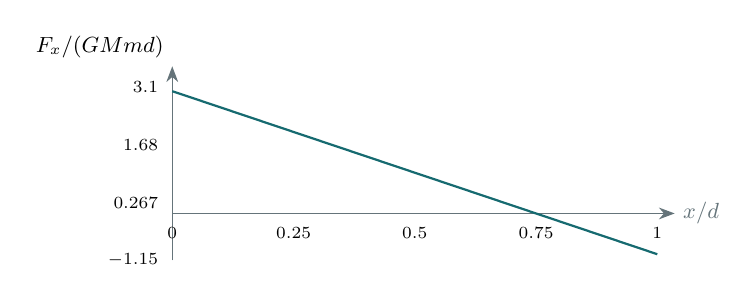
\begin{tikzpicture}[scale=.88,transform shape]
\draw[axis] (0,0.6764706)--(7.25,0.6764706) node[right] {$x/d$};
\draw[axis] (0.0000000,0)--(0.0000000,2.8);
\node[above left] at (0.0000000,2.8) {$F_x/(GMmd)$};
\node[below,font=\scriptsize] at (0.0000000,0.5964706) {$0$};
\node[below,font=\scriptsize] at (1.7500000,0.5964706) {$0.25$};
\node[below,font=\scriptsize] at (3.5000000,0.5964706) {$0.5$};
\node[below,font=\scriptsize] at (5.2500000,0.5964706) {$0.75$};
\node[below,font=\scriptsize] at (7.0000000,0.5964706) {$1$};
\node[left,font=\scriptsize] at (-0.0800000,0.0000000) {$-1.15$};
\node[left,font=\scriptsize] at (-0.0800000,0.8333333) {$0.267$};
\node[left,font=\scriptsize] at (-0.0800000,1.6666667) {$1.68$};
\node[left,font=\scriptsize] at (-0.0800000,2.5000000) {$3.1$};
\draw[thick,color=accent] plot coordinates {(0.0000000,2.4411765) (0.0291667,2.4313725) (0.0583333,2.4215686) (0.0875000,2.4117647) (0.1166667,2.4019608) (0.1458333,2.3921569) (0.1750000,2.3823529) (0.2041667,2.3725490) (0.2333333,2.3627451) (0.2625000,2.3529412) (0.2916667,2.3431373) (0.3208333,2.3333333) (0.3500000,2.3235294) (0.3791667,2.3137255) (0.4083333,2.3039216) (0.4375000,2.2941176) (0.4666667,2.2843137) (0.4958333,2.2745098) (0.5250000,2.2647059) (0.5541667,2.2549020) (0.5833333,2.2450980) (0.6125000,2.2352941) (0.6416667,2.2254902) (0.6708333,2.2156863) (0.7000000,2.2058824) (0.7291667,2.1960784) (0.7583333,2.1862745) (0.7875000,2.1764706) (0.8166667,2.1666667) (0.8458333,2.1568627) (0.8750000,2.1470588) (0.9041667,2.1372549) (0.9333333,2.1274510) (0.9625000,2.1176471) (0.9916667,2.1078431) (1.0208333,2.0980392) (1.0500000,2.0882353) (1.0791667,2.0784314) (1.1083333,2.0686275) (1.1375000,2.0588235) (1.1666667,2.0490196) (1.1958333,2.0392157) (1.2250000,2.0294118) (1.2541667,2.0196078) (1.2833333,2.0098039) (1.3125000,2.0000000) (1.3416667,1.9901961) (1.3708333,1.9803922) (1.4000000,1.9705882) (1.4291667,1.9607843) (1.4583333,1.9509804) (1.4875000,1.9411765) (1.5166667,1.9313725) (1.5458333,1.9215686) (1.5750000,1.9117647) (1.6041667,1.9019608) (1.6333333,1.8921569) (1.6625000,1.8823529) (1.6916667,1.8725490) (1.7208333,1.8627451) (1.7500000,1.8529412) (1.7791667,1.8431373) (1.8083333,1.8333333) (1.8375000,1.8235294) (1.8666667,1.8137255) (1.8958333,1.8039216) (1.9250000,1.7941176) (1.9541667,1.7843137) (1.9833333,1.7745098) (2.0125000,1.7647059) (2.0416667,1.7549020) (2.0708333,1.7450980) (2.1000000,1.7352941) (2.1291667,1.7254902) (2.1583333,1.7156863) (2.1875000,1.7058824) (2.2166667,1.6960784) (2.2458333,1.6862745) (2.2750000,1.6764706) (2.3041667,1.6666667) (2.3333333,1.6568627) (2.3625000,1.6470588) (2.3916667,1.6372549) (2.4208333,1.6274510) (2.4500000,1.6176471) (2.4791667,1.6078431) (2.5083333,1.5980392) (2.5375000,1.5882353) (2.5666667,1.5784314) (2.5958333,1.5686275) (2.6250000,1.5588235) (2.6541667,1.5490196) (2.6833333,1.5392157) (2.7125000,1.5294118) (2.7416667,1.5196078) (2.7708333,1.5098039) (2.8000000,1.5000000) (2.8291667,1.4901961) (2.8583333,1.4803922) (2.8875000,1.4705882) (2.9166667,1.4607843) (2.9458333,1.4509804) (2.9750000,1.4411765) (3.0041667,1.4313725) (3.0333333,1.4215686) (3.0625000,1.4117647) (3.0916667,1.4019608) (3.1208333,1.3921569) (3.1500000,1.3823529) (3.1791667,1.3725490) (3.2083333,1.3627451) (3.2375000,1.3529412) (3.2666667,1.3431373) (3.2958333,1.3333333) (3.3250000,1.3235294) (3.3541667,1.3137255) (3.3833333,1.3039216) (3.4125000,1.2941176) (3.4416667,1.2843137) (3.4708333,1.2745098) (3.5000000,1.2647059) (3.5291667,1.2549020) (3.5583333,1.2450980) (3.5875000,1.2352941) (3.6166667,1.2254902) (3.6458333,1.2156863) (3.6750000,1.2058824) (3.7041667,1.1960784) (3.7333333,1.1862745) (3.7625000,1.1764706) (3.7916667,1.1666667) (3.8208333,1.1568627) (3.8500000,1.1470588) (3.8791667,1.1372549) (3.9083333,1.1274510) (3.9375000,1.1176471) (3.9666667,1.1078431) (3.9958333,1.0980392) (4.0250000,1.0882353) (4.0541667,1.0784314) (4.0833333,1.0686275) (4.1125000,1.0588235) (4.1416667,1.0490196) (4.1708333,1.0392157) (4.2000000,1.0294118) (4.2291667,1.0196078) (4.2583333,1.0098039) (4.2875000,1.0000000) (4.3166667,0.9901961) (4.3458333,0.9803922) (4.3750000,0.9705882) (4.4041667,0.9607843) (4.4333333,0.9509804) (4.4625000,0.9411765) (4.4916667,0.9313725) (4.5208333,0.9215686) (4.5500000,0.9117647) (4.5791667,0.9019608) (4.6083333,0.8921569) (4.6375000,0.8823529) (4.6666667,0.8725490) (4.6958333,0.8627451) (4.7250000,0.8529412) (4.7541667,0.8431373) (4.7833333,0.8333333) (4.8125000,0.8235294) (4.8416667,0.8137255) (4.8708333,0.8039216) (4.9000000,0.7941176) (4.9291667,0.7843137) (4.9583333,0.7745098) (4.9875000,0.7647059) (5.0166667,0.7549020) (5.0458333,0.7450980) (5.0750000,0.7352941) (5.1041667,0.7254902) (5.1333333,0.7156863) (5.1625000,0.7058824) (5.1916667,0.6960784) (5.2208333,0.6862745) (5.2500000,0.6764706) (5.2791667,0.6666667) (5.3083333,0.6568627) (5.3375000,0.6470588) (5.3666667,0.6372549) (5.3958333,0.6274510) (5.4250000,0.6176471) (5.4541667,0.6078431) (5.4833333,0.5980392) (5.5125000,0.5882353) (5.5416667,0.5784314) (5.5708333,0.5686275) (5.6000000,0.5588235) (5.6291667,0.5490196) (5.6583333,0.5392157) (5.6875000,0.5294118) (5.7166667,0.5196078) (5.7458333,0.5098039) (5.7750000,0.5000000) (5.8041667,0.4901961) (5.8333333,0.4803922) (5.8625000,0.4705882) (5.8916667,0.4607843) (5.9208333,0.4509804) (5.9500000,0.4411765) (5.9791667,0.4313725) (6.0083333,0.4215686) (6.0375000,0.4117647) (6.0666667,0.4019608) (6.0958333,0.3921569) (6.1250000,0.3823529) (6.1541667,0.3725490) (6.1833333,0.3627451) (6.2125000,0.3529412) (6.2416667,0.3431373) (6.2708333,0.3333333) (6.3000000,0.3235294) (6.3291667,0.3137255) (6.3583333,0.3039216) (6.3875000,0.2941176) (6.4166667,0.2843137) (6.4458333,0.2745098) (6.4750000,0.2647059) (6.5041667,0.2549020) (6.5333333,0.2450980) (6.5625000,0.2352941) (6.5916667,0.2254902) (6.6208333,0.2156863) (6.6500000,0.2058824) (6.6791667,0.1960784) (6.7083333,0.1862745) (6.7375000,0.1764706) (6.7666667,0.1666667) (6.7958333,0.1568627) (6.8250000,0.1470588) (6.8541667,0.1372549) (6.8833333,0.1274510) (6.9125000,0.1176471) (6.9416667,0.1078431) (6.9708333,0.0980392) (7.0000000,0.0882353)};
\end{tikzpicture}
\figcaption{变图综二.4V2\quad 不等质量的合力零点落在质心}
\end{minipage}\end{center}
\item \textbf{由主轴端点的初值求轨道。}取$\boldsymbol r_0=(a,0)$、$\boldsymbol v_0=(0,\omega b)$，求轨道、角动量和能量。代入矢量解得
\[
x=a\cos\omega t,\quad y=b\sin\omega t,\quad
L_z=mab\omega,\quad E=\tfrac12m\omega^2(a^2+b^2).
\]
图V3取$b=a/2$。$x$在$t=0$取最大，$y$在四分之一周期后取最大，两个振动依次带质点通过椭圆的主轴端。$a=b$给圆，$b\to0$给穿过中心的直线振动。
\begin{center}\begin{minipage}{.98\linewidth}\centering
\begin{tikzpicture}[scale=.88,transform shape]
\draw[axis] (0,1.2500000)--(7.25,1.2500000) node[right] {$\omega t$};
\draw[axis] (0.0000000,0)--(0.0000000,2.8);
\node[above left] at (0.0000000,2.8) {$\text{坐标}/a$};
\node[below,font=\scriptsize] at (0.0000000,1.1700000) {$0$};
\node[below,font=\scriptsize] at (1.7500000,1.1700000) {$1.57$};
\node[below,font=\scriptsize] at (3.5000000,1.1700000) {$3.14$};
\node[below,font=\scriptsize] at (5.2500000,1.1700000) {$4.71$};
\node[below,font=\scriptsize] at (7.0000000,1.1700000) {$6.28$};
\node[left,font=\scriptsize] at (-0.0800000,0.0000000) {$-1.12$};
\node[left,font=\scriptsize] at (-0.0800000,0.8333333) {$-0.373$};
\node[left,font=\scriptsize] at (-0.0800000,1.6666667) {$0.373$};
\node[left,font=\scriptsize] at (-0.0800000,2.5000000) {$1.12$};
\draw[thick,color=accent] plot coordinates {(0.0000000,2.3660714) (0.0291667,2.3656890) (0.0583333,2.3645419) (0.0875000,2.3626310) (0.1166667,2.3599575) (0.1458333,2.3565233) (0.1750000,2.3523307) (0.2041667,2.3473827) (0.2333333,2.3416826) (0.2625000,2.3352343) (0.2916667,2.3280422) (0.3208333,2.3201113) (0.3500000,2.3114470) (0.3791667,2.3020552) (0.4083333,2.2919424) (0.4375000,2.2811155) (0.4666667,2.2695820) (0.4958333,2.2573496) (0.5250000,2.2444269) (0.5541667,2.2308227) (0.5833333,2.2165462) (0.6125000,2.2016073) (0.6416667,2.1860163) (0.6708333,2.1697837) (0.7000000,2.1529208) (0.7291667,2.1354390) (0.7583333,2.1173504) (0.7875000,2.0986674) (0.8166667,2.0794027) (0.8458333,2.0595696) (0.8750000,2.0391817) (0.9041667,2.0182529) (0.9333333,1.9967976) (0.9625000,1.9748304) (0.9916667,1.9523665) (1.0208333,1.9294212) (1.0500000,1.9060103) (1.0791667,1.8821498) (1.1083333,1.8578561) (1.1375000,1.8331457) (1.1666667,1.8080357) (1.1958333,1.7825433) (1.2250000,1.7566858) (1.2541667,1.7304811) (1.2833333,1.7039471) (1.3125000,1.6771020) (1.3416667,1.6499642) (1.3708333,1.6225523) (1.4000000,1.5948850) (1.4291667,1.5669814) (1.4583333,1.5388605) (1.4875000,1.5105417) (1.5166667,1.4820443) (1.5458333,1.4533879) (1.5750000,1.4245920) (1.6041667,1.3956766) (1.6333333,1.3666612) (1.6625000,1.3375660) (1.6916667,1.3084107) (1.7208333,1.2792153) (1.7500000,1.2500000) (1.7791667,1.2207847) (1.8083333,1.1915893) (1.8375000,1.1624340) (1.8666667,1.1333388) (1.8958333,1.1043234) (1.9250000,1.0754080) (1.9541667,1.0466121) (1.9833333,1.0179557) (2.0125000,0.9894583) (2.0416667,0.9611395) (2.0708333,0.9330186) (2.1000000,0.9051150) (2.1291667,0.8774477) (2.1583333,0.8500358) (2.1875000,0.8228980) (2.2166667,0.7960529) (2.2458333,0.7695189) (2.2750000,0.7433142) (2.3041667,0.7174567) (2.3333333,0.6919643) (2.3625000,0.6668543) (2.3916667,0.6421439) (2.4208333,0.6178502) (2.4500000,0.5939897) (2.4791667,0.5705788) (2.5083333,0.5476335) (2.5375000,0.5251696) (2.5666667,0.5032024) (2.5958333,0.4817471) (2.6250000,0.4608183) (2.6541667,0.4404304) (2.6833333,0.4205973) (2.7125000,0.4013326) (2.7416667,0.3826496) (2.7708333,0.3645610) (2.8000000,0.3470792) (2.8291667,0.3302163) (2.8583333,0.3139837) (2.8875000,0.2983927) (2.9166667,0.2834538) (2.9458333,0.2691773) (2.9750000,0.2555731) (3.0041667,0.2426504) (3.0333333,0.2304180) (3.0625000,0.2188845) (3.0916667,0.2080576) (3.1208333,0.1979448) (3.1500000,0.1885530) (3.1791667,0.1798887) (3.2083333,0.1719578) (3.2375000,0.1647657) (3.2666667,0.1583174) (3.2958333,0.1526173) (3.3250000,0.1476693) (3.3541667,0.1434767) (3.3833333,0.1400425) (3.4125000,0.1373690) (3.4416667,0.1354581) (3.4708333,0.1343110) (3.5000000,0.1339286) (3.5291667,0.1343110) (3.5583333,0.1354581) (3.5875000,0.1373690) (3.6166667,0.1400425) (3.6458333,0.1434767) (3.6750000,0.1476693) (3.7041667,0.1526173) (3.7333333,0.1583174) (3.7625000,0.1647657) (3.7916667,0.1719578) (3.8208333,0.1798887) (3.8500000,0.1885530) (3.8791667,0.1979448) (3.9083333,0.2080576) (3.9375000,0.2188845) (3.9666667,0.2304180) (3.9958333,0.2426504) (4.0250000,0.2555731) (4.0541667,0.2691773) (4.0833333,0.2834538) (4.1125000,0.2983927) (4.1416667,0.3139837) (4.1708333,0.3302163) (4.2000000,0.3470792) (4.2291667,0.3645610) (4.2583333,0.3826496) (4.2875000,0.4013326) (4.3166667,0.4205973) (4.3458333,0.4404304) (4.3750000,0.4608183) (4.4041667,0.4817471) (4.4333333,0.5032024) (4.4625000,0.5251696) (4.4916667,0.5476335) (4.5208333,0.5705788) (4.5500000,0.5939897) (4.5791667,0.6178502) (4.6083333,0.6421439) (4.6375000,0.6668543) (4.6666667,0.6919643) (4.6958333,0.7174567) (4.7250000,0.7433142) (4.7541667,0.7695189) (4.7833333,0.7960529) (4.8125000,0.8228980) (4.8416667,0.8500358) (4.8708333,0.8774477) (4.9000000,0.9051150) (4.9291667,0.9330186) (4.9583333,0.9611395) (4.9875000,0.9894583) (5.0166667,1.0179557) (5.0458333,1.0466121) (5.0750000,1.0754080) (5.1041667,1.1043234) (5.1333333,1.1333388) (5.1625000,1.1624340) (5.1916667,1.1915893) (5.2208333,1.2207847) (5.2500000,1.2500000) (5.2791667,1.2792153) (5.3083333,1.3084107) (5.3375000,1.3375660) (5.3666667,1.3666612) (5.3958333,1.3956766) (5.4250000,1.4245920) (5.4541667,1.4533879) (5.4833333,1.4820443) (5.5125000,1.5105417) (5.5416667,1.5388605) (5.5708333,1.5669814) (5.6000000,1.5948850) (5.6291667,1.6225523) (5.6583333,1.6499642) (5.6875000,1.6771020) (5.7166667,1.7039471) (5.7458333,1.7304811) (5.7750000,1.7566858) (5.8041667,1.7825433) (5.8333333,1.8080357) (5.8625000,1.8331457) (5.8916667,1.8578561) (5.9208333,1.8821498) (5.9500000,1.9060103) (5.9791667,1.9294212) (6.0083333,1.9523665) (6.0375000,1.9748304) (6.0666667,1.9967976) (6.0958333,2.0182529) (6.1250000,2.0391817) (6.1541667,2.0595696) (6.1833333,2.0794027) (6.2125000,2.0986674) (6.2416667,2.1173504) (6.2708333,2.1354390) (6.3000000,2.1529208) (6.3291667,2.1697837) (6.3583333,2.1860163) (6.3875000,2.2016073) (6.4166667,2.2165462) (6.4458333,2.2308227) (6.4750000,2.2444269) (6.5041667,2.2573496) (6.5333333,2.2695820) (6.5625000,2.2811155) (6.5916667,2.2919424) (6.6208333,2.3020552) (6.6500000,2.3114470) (6.6791667,2.3201113) (6.7083333,2.3280422) (6.7375000,2.3352343) (6.7666667,2.3416826) (6.7958333,2.3473827) (6.8250000,2.3523307) (6.8541667,2.3565233) (6.8833333,2.3599575) (6.9125000,2.3626310) (6.9416667,2.3645419) (6.9708333,2.3656890) (7.0000000,2.3660714)};
\draw[thick,color=accent] (7.65,2.4)--(8.1,2.4);\node[right,font=\scriptsize] at (8.15,2.4) {$x/a$};
\draw[thick,dashed,color=warm] plot coordinates {(0.0000000,1.2500000) (0.0291667,1.2646077) (0.0583333,1.2792053) (0.0875000,1.2937830) (0.1166667,1.3083306) (0.1458333,1.3228383) (0.1750000,1.3372960) (0.2041667,1.3516939) (0.2333333,1.3660221) (0.2625000,1.3802709) (0.2916667,1.3944303) (0.3208333,1.4084907) (0.3500000,1.4224425) (0.3791667,1.4362761) (0.4083333,1.4499821) (0.4375000,1.4635510) (0.4666667,1.4769736) (0.4958333,1.4902406) (0.5250000,1.5033429) (0.5541667,1.5162716) (0.5833333,1.5290179) (0.6125000,1.5415729) (0.6416667,1.5539280) (0.6708333,1.5660749) (0.7000000,1.5780052) (0.7291667,1.5897106) (0.7583333,1.6011833) (0.7875000,1.6124152) (0.8166667,1.6233988) (0.8458333,1.6341264) (0.8750000,1.6445908) (0.9041667,1.6547848) (0.9333333,1.6647014) (0.9625000,1.6743337) (0.9916667,1.6836752) (1.0208333,1.6927195) (1.0500000,1.7014604) (1.0791667,1.7098918) (1.1083333,1.7180081) (1.1375000,1.7258037) (1.1666667,1.7332731) (1.1958333,1.7404113) (1.2250000,1.7472135) (1.2541667,1.7536748) (1.2833333,1.7597910) (1.3125000,1.7655578) (1.3416667,1.7709712) (1.3708333,1.7760276) (1.4000000,1.7807235) (1.4291667,1.7850557) (1.4583333,1.7890211) (1.4875000,1.7926171) (1.5166667,1.7958413) (1.5458333,1.7986914) (1.5750000,1.8011654) (1.6041667,1.8032616) (1.6333333,1.8049787) (1.6625000,1.8063155) (1.6916667,1.8072709) (1.7208333,1.8078445) (1.7500000,1.8080357) (1.7791667,1.8078445) (1.8083333,1.8072709) (1.8375000,1.8063155) (1.8666667,1.8049787) (1.8958333,1.8032616) (1.9250000,1.8011654) (1.9541667,1.7986914) (1.9833333,1.7958413) (2.0125000,1.7926171) (2.0416667,1.7890211) (2.0708333,1.7850557) (2.1000000,1.7807235) (2.1291667,1.7760276) (2.1583333,1.7709712) (2.1875000,1.7655578) (2.2166667,1.7597910) (2.2458333,1.7536748) (2.2750000,1.7472135) (2.3041667,1.7404113) (2.3333333,1.7332731) (2.3625000,1.7258037) (2.3916667,1.7180081) (2.4208333,1.7098918) (2.4500000,1.7014604) (2.4791667,1.6927195) (2.5083333,1.6836752) (2.5375000,1.6743337) (2.5666667,1.6647014) (2.5958333,1.6547848) (2.6250000,1.6445908) (2.6541667,1.6341264) (2.6833333,1.6233988) (2.7125000,1.6124152) (2.7416667,1.6011833) (2.7708333,1.5897106) (2.8000000,1.5780052) (2.8291667,1.5660749) (2.8583333,1.5539280) (2.8875000,1.5415729) (2.9166667,1.5290179) (2.9458333,1.5162716) (2.9750000,1.5033429) (3.0041667,1.4902406) (3.0333333,1.4769736) (3.0625000,1.4635510) (3.0916667,1.4499821) (3.1208333,1.4362761) (3.1500000,1.4224425) (3.1791667,1.4084907) (3.2083333,1.3944303) (3.2375000,1.3802709) (3.2666667,1.3660221) (3.2958333,1.3516939) (3.3250000,1.3372960) (3.3541667,1.3228383) (3.3833333,1.3083306) (3.4125000,1.2937830) (3.4416667,1.2792053) (3.4708333,1.2646077) (3.5000000,1.2500000) (3.5291667,1.2353923) (3.5583333,1.2207947) (3.5875000,1.2062170) (3.6166667,1.1916694) (3.6458333,1.1771617) (3.6750000,1.1627040) (3.7041667,1.1483061) (3.7333333,1.1339779) (3.7625000,1.1197291) (3.7916667,1.1055697) (3.8208333,1.0915093) (3.8500000,1.0775575) (3.8791667,1.0637239) (3.9083333,1.0500179) (3.9375000,1.0364490) (3.9666667,1.0230264) (3.9958333,1.0097594) (4.0250000,0.9966571) (4.0541667,0.9837284) (4.0833333,0.9709821) (4.1125000,0.9584271) (4.1416667,0.9460720) (4.1708333,0.9339251) (4.2000000,0.9219948) (4.2291667,0.9102894) (4.2583333,0.8988167) (4.2875000,0.8875848) (4.3166667,0.8766012) (4.3458333,0.8658736) (4.3750000,0.8554092) (4.4041667,0.8452152) (4.4333333,0.8352986) (4.4625000,0.8256663) (4.4916667,0.8163248) (4.5208333,0.8072805) (4.5500000,0.7985396) (4.5791667,0.7901082) (4.6083333,0.7819919) (4.6375000,0.7741963) (4.6666667,0.7667269) (4.6958333,0.7595887) (4.7250000,0.7527865) (4.7541667,0.7463252) (4.7833333,0.7402090) (4.8125000,0.7344422) (4.8416667,0.7290288) (4.8708333,0.7239724) (4.9000000,0.7192765) (4.9291667,0.7149443) (4.9583333,0.7109789) (4.9875000,0.7073829) (5.0166667,0.7041587) (5.0458333,0.7013086) (5.0750000,0.6988346) (5.1041667,0.6967384) (5.1333333,0.6950213) (5.1625000,0.6936845) (5.1916667,0.6927291) (5.2208333,0.6921555) (5.2500000,0.6919643) (5.2791667,0.6921555) (5.3083333,0.6927291) (5.3375000,0.6936845) (5.3666667,0.6950213) (5.3958333,0.6967384) (5.4250000,0.6988346) (5.4541667,0.7013086) (5.4833333,0.7041587) (5.5125000,0.7073829) (5.5416667,0.7109789) (5.5708333,0.7149443) (5.6000000,0.7192765) (5.6291667,0.7239724) (5.6583333,0.7290288) (5.6875000,0.7344422) (5.7166667,0.7402090) (5.7458333,0.7463252) (5.7750000,0.7527865) (5.8041667,0.7595887) (5.8333333,0.7667269) (5.8625000,0.7741963) (5.8916667,0.7819919) (5.9208333,0.7901082) (5.9500000,0.7985396) (5.9791667,0.8072805) (6.0083333,0.8163248) (6.0375000,0.8256663) (6.0666667,0.8352986) (6.0958333,0.8452152) (6.1250000,0.8554092) (6.1541667,0.8658736) (6.1833333,0.8766012) (6.2125000,0.8875848) (6.2416667,0.8988167) (6.2708333,0.9102894) (6.3000000,0.9219948) (6.3291667,0.9339251) (6.3583333,0.9460720) (6.3875000,0.9584271) (6.4166667,0.9709821) (6.4458333,0.9837284) (6.4750000,0.9966571) (6.5041667,1.0097594) (6.5333333,1.0230264) (6.5625000,1.0364490) (6.5916667,1.0500179) (6.6208333,1.0637239) (6.6500000,1.0775575) (6.6791667,1.0915093) (6.7083333,1.1055697) (6.7375000,1.1197291) (6.7666667,1.1339779) (6.7958333,1.1483061) (6.8250000,1.1627040) (6.8541667,1.1771617) (6.8833333,1.1916694) (6.9125000,1.2062170) (6.9416667,1.2207947) (6.9708333,1.2353923) (7.0000000,1.2500000)};
\draw[thick,dashed,color=warm] (7.65,1.9)--(8.1,1.9);\node[right,font=\scriptsize] at (8.15,1.9) {$y/a$};
\end{tikzpicture}
\figcaption{变图综二.4V3\quad 两个同频坐标相差四分之一周期}
\end{minipage}\end{center}
\item \textbf{两个方向的频率不同。}设$F_x=-m\omega_x^2x$、$F_y=-m\omega_y^2y$，取$\omega_y=\sqrt2\omega_x$，两个振幅均非零。若存在共同周期，需有$\omega_x T=2\pi n$和$\omega_y T=2\pi j$，因而频率比应是有理数。图V4中的两个坐标各有自己的周期，峰谷的相对位置持续变化。此处没有共同周期，说明得到主问题的闭合椭圆还需要各向同性。
\begin{center}\begin{minipage}{.98\linewidth}\centering
\begin{tikzpicture}[scale=.88,transform shape]
\draw[axis] (0,1.2500000)--(7.25,1.2500000) node[right] {$\omega_xt$};
\draw[axis] (0.0000000,0)--(0.0000000,2.8);
\node[above left] at (0.0000000,2.8) {$\text{归一化坐标}$};
\node[below,font=\scriptsize] at (0.0000000,1.1700000) {$0$};
\node[below,font=\scriptsize] at (1.7500000,1.1700000) {$3.14$};
\node[below,font=\scriptsize] at (3.5000000,1.1700000) {$6.28$};
\node[below,font=\scriptsize] at (5.2500000,1.1700000) {$9.42$};
\node[below,font=\scriptsize] at (7.0000000,1.1700000) {$12.6$};
\node[left,font=\scriptsize] at (-0.0800000,0.0000000) {$-1.1$};
\node[left,font=\scriptsize] at (-0.0800000,0.8333333) {$-0.367$};
\node[left,font=\scriptsize] at (-0.0800000,1.6666667) {$0.367$};
\node[left,font=\scriptsize] at (-0.0800000,2.5000000) {$1.1$};
\draw[thick,color=accent] plot coordinates {(0.0000000,2.3863636) (0.0291667,2.3848063) (0.0583333,2.3801385) (0.0875000,2.3723731) (0.1166667,2.3615314) (0.1458333,2.3476430) (0.1750000,2.3307460) (0.2041667,2.3108868) (0.2333333,2.2881198) (0.2625000,2.2625074) (0.2916667,2.2341198) (0.3208333,2.2030347) (0.3500000,2.1693375) (0.3791667,2.1331204) (0.4083333,2.0944828) (0.4375000,2.0535304) (0.4666667,2.0103757) (0.4958333,1.9651368) (0.5250000,1.9179378) (0.5541667,1.8689080) (0.5833333,1.8181818) (0.6125000,1.7658983) (0.6416667,1.7122007) (0.6708333,1.6572363) (0.7000000,1.6011557) (0.7291667,1.5441126) (0.7583333,1.4862633) (0.7875000,1.4277664) (0.8166667,1.3687823) (0.8458333,1.3094727) (0.8750000,1.2500000) (0.9041667,1.1905273) (0.9333333,1.1312177) (0.9625000,1.0722336) (0.9916667,1.0137367) (1.0208333,0.9558874) (1.0500000,0.8988443) (1.0791667,0.8427637) (1.1083333,0.7877993) (1.1375000,0.7341017) (1.1666667,0.6818182) (1.1958333,0.6310920) (1.2250000,0.5820622) (1.2541667,0.5348632) (1.2833333,0.4896243) (1.3125000,0.4464696) (1.3416667,0.4055172) (1.3708333,0.3668796) (1.4000000,0.3306625) (1.4291667,0.2969653) (1.4583333,0.2658802) (1.4875000,0.2374926) (1.5166667,0.2118802) (1.5458333,0.1891132) (1.5750000,0.1692540) (1.6041667,0.1523570) (1.6333333,0.1384686) (1.6625000,0.1276269) (1.6916667,0.1198615) (1.7208333,0.1151937) (1.7500000,0.1136364) (1.7791667,0.1151937) (1.8083333,0.1198615) (1.8375000,0.1276269) (1.8666667,0.1384686) (1.8958333,0.1523570) (1.9250000,0.1692540) (1.9541667,0.1891132) (1.9833333,0.2118802) (2.0125000,0.2374926) (2.0416667,0.2658802) (2.0708333,0.2969653) (2.1000000,0.3306625) (2.1291667,0.3668796) (2.1583333,0.4055172) (2.1875000,0.4464696) (2.2166667,0.4896243) (2.2458333,0.5348632) (2.2750000,0.5820622) (2.3041667,0.6310920) (2.3333333,0.6818182) (2.3625000,0.7341017) (2.3916667,0.7877993) (2.4208333,0.8427637) (2.4500000,0.8988443) (2.4791667,0.9558874) (2.5083333,1.0137367) (2.5375000,1.0722336) (2.5666667,1.1312177) (2.5958333,1.1905273) (2.6250000,1.2500000) (2.6541667,1.3094727) (2.6833333,1.3687823) (2.7125000,1.4277664) (2.7416667,1.4862633) (2.7708333,1.5441126) (2.8000000,1.6011557) (2.8291667,1.6572363) (2.8583333,1.7122007) (2.8875000,1.7658983) (2.9166667,1.8181818) (2.9458333,1.8689080) (2.9750000,1.9179378) (3.0041667,1.9651368) (3.0333333,2.0103757) (3.0625000,2.0535304) (3.0916667,2.0944828) (3.1208333,2.1331204) (3.1500000,2.1693375) (3.1791667,2.2030347) (3.2083333,2.2341198) (3.2375000,2.2625074) (3.2666667,2.2881198) (3.2958333,2.3108868) (3.3250000,2.3307460) (3.3541667,2.3476430) (3.3833333,2.3615314) (3.4125000,2.3723731) (3.4416667,2.3801385) (3.4708333,2.3848063) (3.5000000,2.3863636) (3.5291667,2.3848063) (3.5583333,2.3801385) (3.5875000,2.3723731) (3.6166667,2.3615314) (3.6458333,2.3476430) (3.6750000,2.3307460) (3.7041667,2.3108868) (3.7333333,2.2881198) (3.7625000,2.2625074) (3.7916667,2.2341198) (3.8208333,2.2030347) (3.8500000,2.1693375) (3.8791667,2.1331204) (3.9083333,2.0944828) (3.9375000,2.0535304) (3.9666667,2.0103757) (3.9958333,1.9651368) (4.0250000,1.9179378) (4.0541667,1.8689080) (4.0833333,1.8181818) (4.1125000,1.7658983) (4.1416667,1.7122007) (4.1708333,1.6572363) (4.2000000,1.6011557) (4.2291667,1.5441126) (4.2583333,1.4862633) (4.2875000,1.4277664) (4.3166667,1.3687823) (4.3458333,1.3094727) (4.3750000,1.2500000) (4.4041667,1.1905273) (4.4333333,1.1312177) (4.4625000,1.0722336) (4.4916667,1.0137367) (4.5208333,0.9558874) (4.5500000,0.8988443) (4.5791667,0.8427637) (4.6083333,0.7877993) (4.6375000,0.7341017) (4.6666667,0.6818182) (4.6958333,0.6310920) (4.7250000,0.5820622) (4.7541667,0.5348632) (4.7833333,0.4896243) (4.8125000,0.4464696) (4.8416667,0.4055172) (4.8708333,0.3668796) (4.9000000,0.3306625) (4.9291667,0.2969653) (4.9583333,0.2658802) (4.9875000,0.2374926) (5.0166667,0.2118802) (5.0458333,0.1891132) (5.0750000,0.1692540) (5.1041667,0.1523570) (5.1333333,0.1384686) (5.1625000,0.1276269) (5.1916667,0.1198615) (5.2208333,0.1151937) (5.2500000,0.1136364) (5.2791667,0.1151937) (5.3083333,0.1198615) (5.3375000,0.1276269) (5.3666667,0.1384686) (5.3958333,0.1523570) (5.4250000,0.1692540) (5.4541667,0.1891132) (5.4833333,0.2118802) (5.5125000,0.2374926) (5.5416667,0.2658802) (5.5708333,0.2969653) (5.6000000,0.3306625) (5.6291667,0.3668796) (5.6583333,0.4055172) (5.6875000,0.4464696) (5.7166667,0.4896243) (5.7458333,0.5348632) (5.7750000,0.5820622) (5.8041667,0.6310920) (5.8333333,0.6818182) (5.8625000,0.7341017) (5.8916667,0.7877993) (5.9208333,0.8427637) (5.9500000,0.8988443) (5.9791667,0.9558874) (6.0083333,1.0137367) (6.0375000,1.0722336) (6.0666667,1.1312177) (6.0958333,1.1905273) (6.1250000,1.2500000) (6.1541667,1.3094727) (6.1833333,1.3687823) (6.2125000,1.4277664) (6.2416667,1.4862633) (6.2708333,1.5441126) (6.3000000,1.6011557) (6.3291667,1.6572363) (6.3583333,1.7122007) (6.3875000,1.7658983) (6.4166667,1.8181818) (6.4458333,1.8689080) (6.4750000,1.9179378) (6.5041667,1.9651368) (6.5333333,2.0103757) (6.5625000,2.0535304) (6.5916667,2.0944828) (6.6208333,2.1331204) (6.6500000,2.1693375) (6.6791667,2.2030347) (6.7083333,2.2341198) (6.7375000,2.2625074) (6.7666667,2.2881198) (6.7958333,2.3108868) (6.8250000,2.3307460) (6.8541667,2.3476430) (6.8833333,2.3615314) (6.9125000,2.3723731) (6.9416667,2.3801385) (6.9708333,2.3848063) (7.0000000,2.3863636)};
\draw[thick,color=accent] (7.65,2.4)--(8.1,2.4);\node[right,font=\scriptsize] at (8.15,2.4) {$x/A$};
\draw[thick,dashed,color=warm] plot coordinates {(0.0000000,1.2500000) (0.0291667,1.3340686) (0.0583333,1.4176765) (0.0875000,1.5003654) (0.1166667,1.5816822) (0.1458333,1.6611811) (0.1750000,1.7384266) (0.2041667,1.8129951) (0.2333333,1.8844781) (0.2625000,1.9524838) (0.2916667,2.0166394) (0.3208333,2.0765934) (0.3500000,2.1320171) (0.3791667,2.1826068) (0.4083333,2.2280853) (0.4375000,2.2682033) (0.4666667,2.3027410) (0.4958333,2.3315089) (0.5250000,2.3543495) (0.5541667,2.3711377) (0.5833333,2.3817813) (0.6125000,2.3862220) (0.6416667,2.3844356) (0.6708333,2.3764318) (0.7000000,2.3622544) (0.7291667,2.3419812) (0.7583333,2.3157233) (0.7875000,2.2836246) (0.8166667,2.2458609) (0.8458333,2.2026394) (0.8750000,2.1541968) (0.9041667,2.1007987) (0.9333333,2.0427377) (0.9625000,1.9803319) (0.9916667,1.9139236) (1.0208333,1.8438765) (1.0500000,1.7705746) (1.0791667,1.6944196) (1.1083333,1.6158290) (1.1375000,1.5352334) (1.1666667,1.4530745) (1.1958333,1.3698027) (1.2250000,1.2858743) (1.2541667,1.2017492) (1.2833333,1.1178886) (1.3125000,1.0347521) (1.3416667,0.9527952) (1.3708333,0.8724672) (1.4000000,0.7942084) (1.4291667,0.7184475) (1.4583333,0.6455999) (1.4875000,0.5760647) (1.5166667,0.5102231) (1.5458333,0.4484360) (1.5750000,0.3910419) (1.6041667,0.3383554) (1.6333333,0.2906653) (1.6625000,0.2482329) (1.6916667,0.2112908) (1.7208333,0.1800415) (1.7500000,0.1546562) (1.7791667,0.1352741) (1.8083333,0.1220013) (1.8375000,0.1149106) (1.8666667,0.1140410) (1.8958333,0.1193970) (1.9250000,0.1309495) (1.9541667,0.1486351) (1.9833333,0.1723568) (2.0125000,0.2019846) (2.0416667,0.2373562) (2.0708333,0.2782777) (2.1000000,0.3245248) (2.1291667,0.3758441) (2.1583333,0.4319543) (2.1875000,0.4925479) (2.2166667,0.5572928) (2.2458333,0.6258342) (2.2750000,0.6977963) (2.3041667,0.7727849) (2.3333333,0.8503889) (2.3625000,0.9301830) (2.3916667,1.0117299) (2.4208333,1.0945827) (2.4500000,1.1782872) (2.4791667,1.2623848) (2.5083333,1.3464145) (2.5375000,1.4299158) (2.5666667,1.5124311) (2.5958333,1.5935080) (2.6250000,1.6727024) (2.6541667,1.7495800) (2.6833333,1.8237197) (2.7125000,1.8947150) (2.7416667,1.9621769) (2.7708333,2.0257356) (2.8000000,2.0850429) (2.8291667,2.1397736) (2.8583333,2.1896277) (2.8875000,2.2343322) (2.9166667,2.2736419) (2.9458333,2.3073415) (2.9750000,2.3352461) (3.0041667,2.3572030) (3.0333333,2.3730917) (3.0625000,2.3828252) (3.0916667,2.3863501) (3.1208333,2.3836471) (3.1500000,2.3747310) (3.1791667,2.3596508) (3.2083333,2.3384889) (3.2375000,2.3113615) (3.2666667,2.2784172) (3.2958333,2.2398365) (3.3250000,2.1958309) (3.3541667,2.1466416) (3.3833333,2.0925382) (3.4125000,2.0338171) (3.4416667,1.9708003) (3.4708333,1.9038330) (3.5000000,1.8332823) (3.5291667,1.7595348) (3.5583333,1.6829948) (3.5875000,1.6040818) (3.6166667,1.5232281) (3.6458333,1.4408770) (3.6750000,1.3574798) (3.7041667,1.2734935) (3.7333333,1.1893784) (3.7625000,1.1055956) (3.7916667,1.0226043) (3.8208333,0.9408591) (3.8500000,0.8608083) (3.8791667,0.7828905) (3.9083333,0.7075327) (3.9375000,0.6351480) (3.9666667,0.5661330) (3.9958333,0.5008661) (4.0250000,0.4397048) (4.0541667,0.3829845) (4.0833333,0.3310159) (4.1125000,0.2840839) (4.1416667,0.2424458) (4.1708333,0.2063296) (4.2000000,0.1759334) (4.2291667,0.1514237) (4.2583333,0.1329349) (4.2875000,0.1205683) (4.3166667,0.1143917) (4.3458333,0.1144389) (4.3750000,0.1207097) (4.4041667,0.1331696) (4.4333333,0.1517505) (4.4625000,0.1763504) (4.4916667,0.2068346) (4.5208333,0.2430360) (4.5500000,0.2847562) (4.5791667,0.3317664) (4.6083333,0.3838092) (4.6375000,0.4405992) (4.6666667,0.5018252) (4.6958333,0.5671517) (4.7250000,0.6362206) (4.7541667,0.7086534) (4.7833333,0.7840531) (4.8125000,0.8620064) (4.8416667,0.9420862) (4.8708333,1.0238536) (4.9000000,1.1068604) (4.9291667,1.1906516) (4.9583333,1.2747682) (4.9875000,1.3587490) (5.0166667,1.4421337) (5.0458333,1.5244655) (5.0750000,1.6052930) (5.1041667,1.6841733) (5.1333333,1.7606741) (5.1625000,1.8343761) (5.1916667,1.9048753) (5.2208333,1.9717855) (5.2500000,2.0347397) (5.2791667,2.0933932) (5.3083333,2.1474243) (5.3375000,2.1965370) (5.3666667,2.2404621) (5.3958333,2.2789589) (5.4250000,2.3118164) (5.4541667,2.3388544) (5.4833333,2.3599249) (5.5125000,2.3749123) (5.5416667,2.3837345) (5.5708333,2.3863431) (5.6000000,2.3827239) (5.6291667,2.3728967) (5.6583333,2.3569153) (5.6875000,2.3348673) (5.7166667,2.3068737) (5.7458333,2.2730877) (5.7750000,2.2336945) (5.8041667,2.1889101) (5.8333333,2.1389799) (5.8625000,2.0841776) (5.8916667,2.0248035) (5.9208333,1.9611829) (5.9500000,1.8936647) (5.9791667,1.8226188) (6.0083333,1.7484346) (6.0375000,1.6715186) (6.0666667,1.5922925) (6.0958333,1.5111904) (6.1250000,1.4286568) (6.1541667,1.3451441) (6.1833333,1.2611099) (6.2125000,1.1770149) (6.2416667,1.0933198) (6.2708333,1.0104834) (6.3000000,0.9289598) (6.3291667,0.8491956) (6.3583333,0.7716281) (6.3875000,0.6966824) (6.4166667,0.6247691) (6.4458333,0.5562826) (6.4750000,0.4915980) (6.5041667,0.4310699) (6.5333333,0.3750301) (6.5625000,0.3237856) (6.5916667,0.2776173) (6.6208333,0.2367783) (6.6500000,0.2014924) (6.6791667,0.1719529) (6.7083333,0.1483218) (6.7375000,0.1307285) (6.7666667,0.1192695) (6.7958333,0.1140077) (6.8250000,0.1149717) (6.8541667,0.1221564) (6.8833333,0.1355224) (6.9125000,0.1549964) (6.9416667,0.1804716) (6.9708333,0.2118086) (7.0000000,0.2488354)};
\draw[thick,dashed,color=warm] (7.65,1.9)--(8.1,1.9);\node[right,font=\scriptsize] at (8.15,1.9) {$y/B$};
\end{tikzpicture}
\figcaption{变图综二.4V4\quad 非同频的两个振动没有共同周期}
\end{minipage}\end{center}
\item \textbf{源组整体匀速平移。}各源的相对位置固定，质心以速度$U$沿$x$正方向移动。取$R_{C,x}(0)=0$，记$\omega=\sqrt{GM_{\rm tot}}$，令$\boldsymbol\rho=\boldsymbol r-\boldsymbol R_C(t)$。因$\ddot{\boldsymbol R}_C=0$，相对方程仍为$\ddot{\boldsymbol\rho}=-\omega^2\boldsymbol\rho$。若相对$x$坐标的初值为$a$，相对$x$速度初值为零，则
\[
x/a=(U/(a\omega))\omega t+\cos\omega t.
\]
图V5取$U=a\omega/4$，振荡曲线围绕匀速移动的质心线。相对椭圆每过$2\pi/\omega$回到同一相位，地面系的位置每周期前移$2\pi U/\omega$。
\begin{center}\begin{minipage}{.98\linewidth}\centering
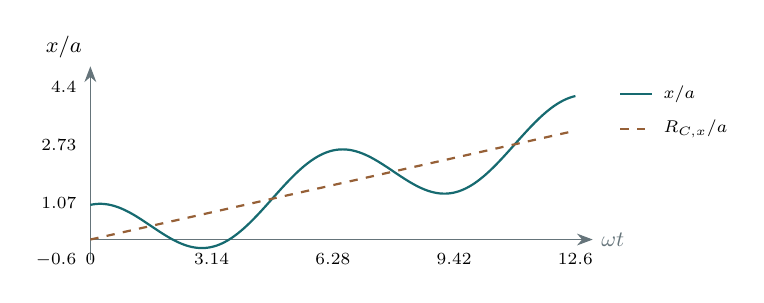
\begin{tikzpicture}[scale=.88,transform shape]
\draw[axis] (0,0.3000000)--(7.25,0.3000000) node[right] {$\omega t$};
\draw[axis] (0.0000000,0)--(0.0000000,2.8);
\node[above left] at (0.0000000,2.8) {$x/a$};
\node[below,font=\scriptsize] at (0.0000000,0.2200000) {$0$};
\node[below,font=\scriptsize] at (1.7500000,0.2200000) {$3.14$};
\node[below,font=\scriptsize] at (3.5000000,0.2200000) {$6.28$};
\node[below,font=\scriptsize] at (5.2500000,0.2200000) {$9.42$};
\node[below,font=\scriptsize] at (7.0000000,0.2200000) {$12.6$};
\node[left,font=\scriptsize] at (-0.0800000,0.0000000) {$-0.6$};
\node[left,font=\scriptsize] at (-0.0800000,0.8333333) {$1.07$};
\node[left,font=\scriptsize] at (-0.0800000,1.6666667) {$2.73$};
\node[left,font=\scriptsize] at (-0.0800000,2.5000000) {$4.4$};
\draw[thick,color=accent] plot coordinates {(0.0000000,0.8000000) (0.0291667,0.8058598) (0.0583333,0.8103509) (0.0875000,0.8134791) (0.1166667,0.8152537) (0.1458333,0.8156878) (0.1750000,0.8147982) (0.2041667,0.8126051) (0.2333333,0.8091326) (0.2625000,0.8044081) (0.2916667,0.7984625) (0.3208333,0.7913301) (0.3500000,0.7830483) (0.3791667,0.7736578) (0.4083333,0.7632022) (0.4375000,0.7517282) (0.4666667,0.7392851) (0.4958333,0.7259249) (0.5250000,0.7117024) (0.5541667,0.6966742) (0.5833333,0.6808997) (0.6125000,0.6644399) (0.6416667,0.6473580) (0.6708333,0.6297186) (0.7000000,0.6115881) (0.7291667,0.5930341) (0.7583333,0.5741254) (0.7875000,0.5549318) (0.8166667,0.5355238) (0.8458333,0.5159725) (0.8750000,0.4963495) (0.9041667,0.4767265) (0.9333333,0.4571753) (0.9625000,0.4377673) (0.9916667,0.4185736) (1.0208333,0.3996649) (1.0500000,0.3811110) (1.0791667,0.3629805) (1.1083333,0.3453411) (1.1375000,0.3282592) (1.1666667,0.3117994) (1.1958333,0.2960249) (1.2250000,0.2809967) (1.2541667,0.2667741) (1.2833333,0.2534140) (1.3125000,0.2409709) (1.3416667,0.2294969) (1.3708333,0.2190413) (1.4000000,0.2096508) (1.4291667,0.2013690) (1.4583333,0.1942365) (1.4875000,0.1882910) (1.5166667,0.1835665) (1.5458333,0.1800940) (1.5750000,0.1779009) (1.6041667,0.1770112) (1.6333333,0.1774453) (1.6625000,0.1792200) (1.6916667,0.1823482) (1.7208333,0.1868393) (1.7500000,0.1926991) (1.7791667,0.1999293) (1.8083333,0.2085281) (1.8375000,0.2184899) (1.8666667,0.2298052) (1.8958333,0.2424611) (1.9250000,0.2564407) (1.9541667,0.2717238) (1.9833333,0.2882862) (2.0125000,0.3061007) (2.0416667,0.3251362) (2.0708333,0.3453586) (2.1000000,0.3667304) (2.1291667,0.3892109) (2.1583333,0.4127565) (2.1875000,0.4373205) (2.2166667,0.4628535) (2.2458333,0.4893036) (2.2750000,0.5166162) (2.3041667,0.5447343) (2.3333333,0.5735988) (2.3625000,0.6031485) (2.3916667,0.6333204) (2.4208333,0.6640498) (2.4500000,0.6952702) (2.4791667,0.7269142) (2.5083333,0.7589128) (2.5375000,0.7911964) (2.5666667,0.8236944) (2.5958333,0.8563357) (2.6250000,0.8890486) (2.6541667,0.9217616) (2.6833333,0.9544028) (2.7125000,0.9869008) (2.7416667,1.0191844) (2.7708333,1.0511831) (2.8000000,1.0828270) (2.8291667,1.1140475) (2.8583333,1.1447768) (2.8875000,1.1749487) (2.9166667,1.2044985) (2.9458333,1.2333630) (2.9750000,1.2614811) (3.0041667,1.2887936) (3.0333333,1.3152437) (3.0625000,1.3407768) (3.0916667,1.3653408) (3.1208333,1.3888863) (3.1500000,1.4113668) (3.1791667,1.4327386) (3.2083333,1.4529610) (3.2375000,1.4719966) (3.2666667,1.4898110) (3.2958333,1.5063735) (3.3250000,1.5216565) (3.3541667,1.5356362) (3.3833333,1.5482920) (3.4125000,1.5596074) (3.4416667,1.5695691) (3.4708333,1.5781679) (3.5000000,1.5853982) (3.5291667,1.5912579) (3.5583333,1.5957491) (3.5875000,1.5988773) (3.6166667,1.6006519) (3.6458333,1.6010860) (3.6750000,1.6001963) (3.7041667,1.5980033) (3.7333333,1.5945308) (3.7625000,1.5898063) (3.7916667,1.5838607) (3.8208333,1.5767283) (3.8500000,1.5684465) (3.8791667,1.5590559) (3.9083333,1.5486004) (3.9375000,1.5371263) (3.9666667,1.5246832) (3.9958333,1.5113231) (4.0250000,1.4971005) (4.0541667,1.4820724) (4.0833333,1.4662979) (4.1125000,1.4498381) (4.1416667,1.4327561) (4.1708333,1.4151168) (4.2000000,1.3969863) (4.2291667,1.3784323) (4.2583333,1.3595236) (4.2875000,1.3403300) (4.3166667,1.3209220) (4.3458333,1.3013707) (4.3750000,1.2817477) (4.4041667,1.2621247) (4.4333333,1.2425734) (4.4625000,1.2231654) (4.4916667,1.2039718) (4.5208333,1.1850631) (4.5500000,1.1665091) (4.5791667,1.1483786) (4.6083333,1.1307393) (4.6375000,1.1136573) (4.6666667,1.0971976) (4.6958333,1.0814230) (4.7250000,1.0663949) (4.7541667,1.0521723) (4.7833333,1.0388122) (4.8125000,1.0263691) (4.8416667,1.0148950) (4.8708333,1.0044395) (4.9000000,0.9950489) (4.9291667,0.9867671) (4.9583333,0.9796347) (4.9875000,0.9736891) (5.0166667,0.9689646) (5.0458333,0.9654921) (5.0750000,0.9632991) (5.1041667,0.9624094) (5.1333333,0.9628435) (5.1625000,0.9646181) (5.1916667,0.9677463) (5.2208333,0.9722375) (5.2500000,0.9780972) (5.2791667,0.9853275) (5.3083333,0.9939263) (5.3375000,1.0038880) (5.3666667,1.0152034) (5.3958333,1.0278593) (5.4250000,1.0418389) (5.4541667,1.0571219) (5.4833333,1.0736844) (5.5125000,1.0914988) (5.5416667,1.1105344) (5.5708333,1.1307568) (5.6000000,1.1521286) (5.6291667,1.1746091) (5.6583333,1.1981546) (5.6875000,1.2227186) (5.7166667,1.2482517) (5.7458333,1.2747018) (5.7750000,1.3020143) (5.8041667,1.3301324) (5.8333333,1.3589969) (5.8625000,1.3885467) (5.8916667,1.4187186) (5.9208333,1.4494479) (5.9500000,1.4806684) (5.9791667,1.5123123) (6.0083333,1.5443110) (6.0375000,1.5765946) (6.0666667,1.6090926) (6.0958333,1.6417338) (6.1250000,1.6744468) (6.1541667,1.7071597) (6.1833333,1.7398010) (6.2125000,1.7722990) (6.2416667,1.8045826) (6.2708333,1.8365812) (6.3000000,1.8682252) (6.3291667,1.8994457) (6.3583333,1.9301750) (6.3875000,1.9603469) (6.4166667,1.9898966) (6.4458333,2.0187611) (6.4750000,2.0468792) (6.5041667,2.0741918) (6.5333333,2.1006419) (6.5625000,2.1261749) (6.5916667,2.1507390) (6.6208333,2.1742845) (6.6500000,2.1967650) (6.6791667,2.2181368) (6.7083333,2.2383592) (6.7375000,2.2573947) (6.7666667,2.2752092) (6.7958333,2.2917716) (6.8250000,2.3070547) (6.8541667,2.3210343) (6.8833333,2.3336902) (6.9125000,2.3450055) (6.9416667,2.3549673) (6.9708333,2.3635661) (7.0000000,2.3707963)};
\draw[thick,color=accent] (7.65,2.4)--(8.1,2.4);\node[right,font=\scriptsize] at (8.15,2.4) {$x/a$};
\draw[thick,dashed,color=warm] plot coordinates {(0.0000000,0.3000000) (0.0291667,0.3065450) (0.0583333,0.3130900) (0.0875000,0.3196350) (0.1166667,0.3261799) (0.1458333,0.3327249) (0.1750000,0.3392699) (0.2041667,0.3458149) (0.2333333,0.3523599) (0.2625000,0.3589049) (0.2916667,0.3654498) (0.3208333,0.3719948) (0.3500000,0.3785398) (0.3791667,0.3850848) (0.4083333,0.3916298) (0.4375000,0.3981748) (0.4666667,0.4047198) (0.4958333,0.4112647) (0.5250000,0.4178097) (0.5541667,0.4243547) (0.5833333,0.4308997) (0.6125000,0.4374447) (0.6416667,0.4439897) (0.6708333,0.4505346) (0.7000000,0.4570796) (0.7291667,0.4636246) (0.7583333,0.4701696) (0.7875000,0.4767146) (0.8166667,0.4832596) (0.8458333,0.4898046) (0.8750000,0.4963495) (0.9041667,0.5028945) (0.9333333,0.5094395) (0.9625000,0.5159845) (0.9916667,0.5225295) (1.0208333,0.5290745) (1.0500000,0.5356194) (1.0791667,0.5421644) (1.1083333,0.5487094) (1.1375000,0.5552544) (1.1666667,0.5617994) (1.1958333,0.5683444) (1.2250000,0.5748894) (1.2541667,0.5814343) (1.2833333,0.5879793) (1.3125000,0.5945243) (1.3416667,0.6010693) (1.3708333,0.6076143) (1.4000000,0.6141593) (1.4291667,0.6207043) (1.4583333,0.6272492) (1.4875000,0.6337942) (1.5166667,0.6403392) (1.5458333,0.6468842) (1.5750000,0.6534292) (1.6041667,0.6599742) (1.6333333,0.6665191) (1.6625000,0.6730641) (1.6916667,0.6796091) (1.7208333,0.6861541) (1.7500000,0.6926991) (1.7791667,0.6992441) (1.8083333,0.7057891) (1.8375000,0.7123340) (1.8666667,0.7188790) (1.8958333,0.7254240) (1.9250000,0.7319690) (1.9541667,0.7385140) (1.9833333,0.7450590) (2.0125000,0.7516039) (2.0416667,0.7581489) (2.0708333,0.7646939) (2.1000000,0.7712389) (2.1291667,0.7777839) (2.1583333,0.7843289) (2.1875000,0.7908739) (2.2166667,0.7974188) (2.2458333,0.8039638) (2.2750000,0.8105088) (2.3041667,0.8170538) (2.3333333,0.8235988) (2.3625000,0.8301438) (2.3916667,0.8366887) (2.4208333,0.8432337) (2.4500000,0.8497787) (2.4791667,0.8563237) (2.5083333,0.8628687) (2.5375000,0.8694137) (2.5666667,0.8759587) (2.5958333,0.8825036) (2.6250000,0.8890486) (2.6541667,0.8955936) (2.6833333,0.9021386) (2.7125000,0.9086836) (2.7416667,0.9152286) (2.7708333,0.9217735) (2.8000000,0.9283185) (2.8291667,0.9348635) (2.8583333,0.9414085) (2.8875000,0.9479535) (2.9166667,0.9544985) (2.9458333,0.9610435) (2.9750000,0.9675884) (3.0041667,0.9741334) (3.0333333,0.9806784) (3.0625000,0.9872234) (3.0916667,0.9937684) (3.1208333,1.0003134) (3.1500000,1.0068583) (3.1791667,1.0134033) (3.2083333,1.0199483) (3.2375000,1.0264933) (3.2666667,1.0330383) (3.2958333,1.0395833) (3.3250000,1.0461283) (3.3541667,1.0526732) (3.3833333,1.0592182) (3.4125000,1.0657632) (3.4416667,1.0723082) (3.4708333,1.0788532) (3.5000000,1.0853982) (3.5291667,1.0919431) (3.5583333,1.0984881) (3.5875000,1.1050331) (3.6166667,1.1115781) (3.6458333,1.1181231) (3.6750000,1.1246681) (3.7041667,1.1312131) (3.7333333,1.1377580) (3.7625000,1.1443030) (3.7916667,1.1508480) (3.8208333,1.1573930) (3.8500000,1.1639380) (3.8791667,1.1704830) (3.9083333,1.1770279) (3.9375000,1.1835729) (3.9666667,1.1901179) (3.9958333,1.1966629) (4.0250000,1.2032079) (4.0541667,1.2097529) (4.0833333,1.2162979) (4.1125000,1.2228428) (4.1416667,1.2293878) (4.1708333,1.2359328) (4.2000000,1.2424778) (4.2291667,1.2490228) (4.2583333,1.2555678) (4.2875000,1.2621128) (4.3166667,1.2686577) (4.3458333,1.2752027) (4.3750000,1.2817477) (4.4041667,1.2882927) (4.4333333,1.2948377) (4.4625000,1.3013827) (4.4916667,1.3079276) (4.5208333,1.3144726) (4.5500000,1.3210176) (4.5791667,1.3275626) (4.6083333,1.3341076) (4.6375000,1.3406526) (4.6666667,1.3471976) (4.6958333,1.3537425) (4.7250000,1.3602875) (4.7541667,1.3668325) (4.7833333,1.3733775) (4.8125000,1.3799225) (4.8416667,1.3864675) (4.8708333,1.3930124) (4.9000000,1.3995574) (4.9291667,1.4061024) (4.9583333,1.4126474) (4.9875000,1.4191924) (5.0166667,1.4257374) (5.0458333,1.4322824) (5.0750000,1.4388273) (5.1041667,1.4453723) (5.1333333,1.4519173) (5.1625000,1.4584623) (5.1916667,1.4650073) (5.2208333,1.4715523) (5.2500000,1.4780972) (5.2791667,1.4846422) (5.3083333,1.4911872) (5.3375000,1.4977322) (5.3666667,1.5042772) (5.3958333,1.5108222) (5.4250000,1.5173672) (5.4541667,1.5239121) (5.4833333,1.5304571) (5.5125000,1.5370021) (5.5416667,1.5435471) (5.5708333,1.5500921) (5.6000000,1.5566371) (5.6291667,1.5631820) (5.6583333,1.5697270) (5.6875000,1.5762720) (5.7166667,1.5828170) (5.7458333,1.5893620) (5.7750000,1.5959070) (5.8041667,1.6024520) (5.8333333,1.6089969) (5.8625000,1.6155419) (5.8916667,1.6220869) (5.9208333,1.6286319) (5.9500000,1.6351769) (5.9791667,1.6417219) (6.0083333,1.6482668) (6.0375000,1.6548118) (6.0666667,1.6613568) (6.0958333,1.6679018) (6.1250000,1.6744468) (6.1541667,1.6809918) (6.1833333,1.6875368) (6.2125000,1.6940817) (6.2416667,1.7006267) (6.2708333,1.7071717) (6.3000000,1.7137167) (6.3291667,1.7202617) (6.3583333,1.7268067) (6.3875000,1.7333516) (6.4166667,1.7398966) (6.4458333,1.7464416) (6.4750000,1.7529866) (6.5041667,1.7595316) (6.5333333,1.7660766) (6.5625000,1.7726216) (6.5916667,1.7791665) (6.6208333,1.7857115) (6.6500000,1.7922565) (6.6791667,1.7988015) (6.7083333,1.8053465) (6.7375000,1.8118915) (6.7666667,1.8184364) (6.7958333,1.8249814) (6.8250000,1.8315264) (6.8541667,1.8380714) (6.8833333,1.8446164) (6.9125000,1.8511614) (6.9416667,1.8577064) (6.9708333,1.8642513) (7.0000000,1.8707963)};
\draw[thick,dashed,color=warm] (7.65,1.9)--(8.1,1.9);\node[right,font=\scriptsize] at (8.15,1.9) {$R_{C,x}/a$};
\end{tikzpicture}
\figcaption{变图综二.4V5\quad 整体平移的质心线和相对振动}
\end{minipage}\end{center}
\item \textbf{沿椭圆哪一处最快。}半轴为$a>b$。由中心势能与总能量，
\[
v^2=\omega^2(a^2+b^2-r^2).
\]
所以在短轴端$r=b$处$v_{\max}=\omega a$，长轴端$r=a$处$v_{\min}=\omega b$。图V6取$b=a/2$，横轴从短轴端到长轴端，纵轴从1降到$1/2$。两个端点处速度分别垂直矢径，乘上对应$r$都给$r v=ab\omega$，与恒定面积速度相合。
\begin{center}\begin{minipage}{.98\linewidth}\centering
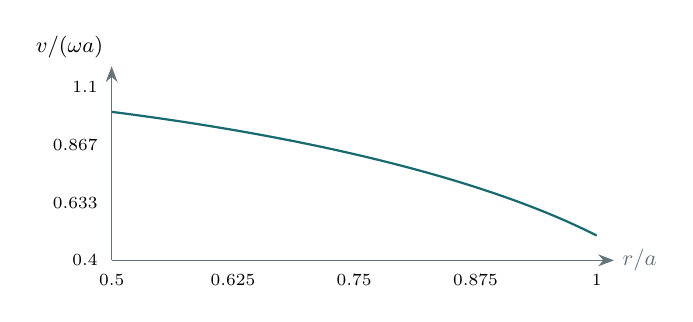
\begin{tikzpicture}[scale=.88,transform shape]
\draw[axis] (0,0.0000000)--(7.25,0.0000000) node[right] {$r/a$};
\draw[axis] (0.0000000,0)--(0.0000000,2.8);
\node[above left] at (0.0000000,2.8) {$v/(\omega a)$};
\node[below,font=\scriptsize] at (0.0000000,-0.0800000) {$0.5$};
\node[below,font=\scriptsize] at (1.7500000,-0.0800000) {$0.625$};
\node[below,font=\scriptsize] at (3.5000000,-0.0800000) {$0.75$};
\node[below,font=\scriptsize] at (5.2500000,-0.0800000) {$0.875$};
\node[below,font=\scriptsize] at (7.0000000,-0.0800000) {$1$};
\node[left,font=\scriptsize] at (-0.0800000,0.0000000) {$0.4$};
\node[left,font=\scriptsize] at (-0.0800000,0.8333333) {$0.633$};
\node[left,font=\scriptsize] at (-0.0800000,1.6666667) {$0.867$};
\node[left,font=\scriptsize] at (-0.0800000,2.5000000) {$1.1$};
\draw[thick,color=accent] plot coordinates {(0.0000000,2.1428571) (0.0291667,2.1391272) (0.0583333,2.1353778) (0.0875000,2.1316090) (0.1166667,2.1278205) (0.1458333,2.1240125) (0.1750000,2.1201847) (0.2041667,2.1163372) (0.2333333,2.1124699) (0.2625000,2.1085827) (0.2916667,2.1046756) (0.3208333,2.1007485) (0.3500000,2.0968013) (0.3791667,2.0928339) (0.4083333,2.0888463) (0.4375000,2.0848384) (0.4666667,2.0808102) (0.4958333,2.0767616) (0.5250000,2.0726925) (0.5541667,2.0686028) (0.5833333,2.0644924) (0.6125000,2.0603614) (0.6416667,2.0562096) (0.6708333,2.0520369) (0.7000000,2.0478433) (0.7291667,2.0436286) (0.7583333,2.0393929) (0.7875000,2.0351361) (0.8166667,2.0308580) (0.8458333,2.0265585) (0.8750000,2.0222377) (0.9041667,2.0178954) (0.9333333,2.0135315) (0.9625000,2.0091460) (0.9916667,2.0047387) (1.0208333,2.0003097) (1.0500000,1.9958587) (1.0791667,1.9913858) (1.1083333,1.9868908) (1.1375000,1.9823737) (1.1666667,1.9778343) (1.1958333,1.9732725) (1.2250000,1.9686884) (1.2541667,1.9640817) (1.2833333,1.9594525) (1.3125000,1.9548005) (1.3416667,1.9501258) (1.3708333,1.9454282) (1.4000000,1.9407075) (1.4291667,1.9359639) (1.4583333,1.9311970) (1.4875000,1.9264069) (1.5166667,1.9215933) (1.5458333,1.9167564) (1.5750000,1.9118958) (1.6041667,1.9070116) (1.6333333,1.9021035) (1.6625000,1.8971716) (1.6916667,1.8922157) (1.7208333,1.8872357) (1.7500000,1.8822315) (1.7791667,1.8772029) (1.8083333,1.8721499) (1.8375000,1.8670724) (1.8666667,1.8619702) (1.8958333,1.8568433) (1.9250000,1.8516914) (1.9541667,1.8465146) (1.9833333,1.8413126) (2.0125000,1.8360854) (2.0416667,1.8308328) (2.0708333,1.8255547) (2.1000000,1.8202510) (2.1291667,1.8149215) (2.1583333,1.8095662) (2.1875000,1.8041849) (2.2166667,1.7987775) (2.2458333,1.7933438) (2.2750000,1.7878837) (2.3041667,1.7823971) (2.3333333,1.7768838) (2.3625000,1.7713437) (2.3916667,1.7657767) (2.4208333,1.7601826) (2.4500000,1.7545613) (2.4791667,1.7489127) (2.5083333,1.7432365) (2.5375000,1.7375326) (2.5666667,1.7318009) (2.5958333,1.7260413) (2.6250000,1.7202536) (2.6541667,1.7144375) (2.6833333,1.7085931) (2.7125000,1.7027201) (2.7416667,1.6968183) (2.7708333,1.6908876) (2.8000000,1.6849278) (2.8291667,1.6789388) (2.8583333,1.6729204) (2.8875000,1.6668723) (2.9166667,1.6607946) (2.9458333,1.6546869) (2.9750000,1.6485490) (3.0041667,1.6423809) (3.0333333,1.6361823) (3.0625000,1.6299530) (3.0916667,1.6236929) (3.1208333,1.6174018) (3.1500000,1.6110794) (3.1791667,1.6047256) (3.2083333,1.5983401) (3.2375000,1.5919228) (3.2666667,1.5854735) (3.2958333,1.5789920) (3.3250000,1.5724780) (3.3541667,1.5659314) (3.3833333,1.5593519) (3.4125000,1.5527393) (3.4416667,1.5460934) (3.4708333,1.5394139) (3.5000000,1.5327007) (3.5291667,1.5259535) (3.5583333,1.5191721) (3.5875000,1.5123562) (3.6166667,1.5055056) (3.6458333,1.4986201) (3.6750000,1.4916994) (3.7041667,1.4847432) (3.7333333,1.4777513) (3.7625000,1.4707235) (3.7916667,1.4636595) (3.8208333,1.4565590) (3.8500000,1.4494217) (3.8791667,1.4422474) (3.9083333,1.4350358) (3.9375000,1.4277866) (3.9666667,1.4204995) (3.9958333,1.4131743) (4.0250000,1.4058106) (4.0541667,1.3984081) (4.0833333,1.3909666) (4.1125000,1.3834857) (4.1416667,1.3759650) (4.1708333,1.3684044) (4.2000000,1.3608035) (4.2291667,1.3531618) (4.2583333,1.3454792) (4.2875000,1.3377552) (4.3166667,1.3299895) (4.3458333,1.3221818) (4.3750000,1.3143316) (4.4041667,1.3064387) (4.4333333,1.2985027) (4.4625000,1.2905231) (4.4916667,1.2824996) (4.5208333,1.2744318) (4.5500000,1.2663193) (4.5791667,1.2581618) (4.6083333,1.2499587) (4.6375000,1.2417096) (4.6666667,1.2334143) (4.6958333,1.2250721) (4.7250000,1.2166827) (4.7541667,1.2082456) (4.7833333,1.1997603) (4.8125000,1.1912265) (4.8416667,1.1826435) (4.8708333,1.1740110) (4.9000000,1.1653284) (4.9291667,1.1565952) (4.9583333,1.1478110) (4.9875000,1.1389751) (5.0166667,1.1300871) (5.0458333,1.1211463) (5.0750000,1.1121524) (5.1041667,1.1031046) (5.1333333,1.0940024) (5.1625000,1.0848452) (5.1916667,1.0756324) (5.2208333,1.0663635) (5.2500000,1.0570377) (5.2791667,1.0476544) (5.3083333,1.0382129) (5.3375000,1.0287127) (5.3666667,1.0191530) (5.3958333,1.0095331) (5.4250000,0.9998523) (5.4541667,0.9901098) (5.4833333,0.9803050) (5.5125000,0.9704370) (5.5416667,0.9605051) (5.5708333,0.9505085) (5.6000000,0.9404463) (5.6291667,0.9303177) (5.6583333,0.9201219) (5.6875000,0.9098579) (5.7166667,0.8995249) (5.7458333,0.8891220) (5.7750000,0.8786481) (5.8041667,0.8681024) (5.8333333,0.8574839) (5.8625000,0.8467914) (5.8916667,0.8360240) (5.9208333,0.8251806) (5.9500000,0.8142601) (5.9791667,0.8032614) (6.0083333,0.7921833) (6.0375000,0.7810245) (6.0666667,0.7697840) (6.0958333,0.7584603) (6.1250000,0.7470523) (6.1541667,0.7355586) (6.1833333,0.7239778) (6.2125000,0.7123084) (6.2416667,0.7005491) (6.2708333,0.6886984) (6.3000000,0.6767547) (6.3291667,0.6647163) (6.3583333,0.6525818) (6.3875000,0.6403493) (6.4166667,0.6280171) (6.4458333,0.6155835) (6.4750000,0.6030465) (6.5041667,0.5904042) (6.5333333,0.5776547) (6.5625000,0.5647959) (6.5916667,0.5518256) (6.6208333,0.5387417) (6.6500000,0.5255418) (6.6791667,0.5122237) (6.7083333,0.4987848) (6.7375000,0.4852226) (6.7666667,0.4715345) (6.7958333,0.4577177) (6.8250000,0.4437694) (6.8541667,0.4296866) (6.8833333,0.4154662) (6.9125000,0.4011051) (6.9416667,0.3865998) (6.9708333,0.3719469) (7.0000000,0.3571429)};
\end{tikzpicture}
\figcaption{变图综二.4V6\quad 速率由短轴端向长轴端下降}
\end{minipage}\end{center}
\item \textbf{允许两物体同时运动。}质量为$M,m$的两物体只受彼此的线性引力。对$\boldsymbol\rho=\boldsymbol r_m-\boldsymbol r_M$相减两条加速度方程，得
\[
\ddot{\boldsymbol\rho}=-G(M+m)\boldsymbol\rho,\qquad
\frac{T_{\rm relative}}{T_{\rm fixed}}=\frac1{\sqrt{1+m/M}}.
\]
图V7在$m/M\to0$时趋于1，等质量处为$1/\sqrt2$。质心参考系中的两条椭圆分别是相对椭圆乘$M/(M+m)$与$-m/(M+m)$，所以周期相同。
\begin{center}\begin{minipage}{.98\linewidth}\centering
\begin{tikzpicture}[scale=.88,transform shape]
\draw[axis] (0,0.0000000)--(7.25,0.0000000) node[right] {$m/M$};
\draw[axis] (0.0000000,0)--(0.0000000,2.8);
\node[above left] at (0.0000000,2.8) {$T_{\rm relative}/T_{\rm fixed}$};
\node[below,font=\scriptsize] at (0.0000000,-0.0800000) {$0$};
\node[below,font=\scriptsize] at (1.7500000,-0.0800000) {$0.375$};
\node[below,font=\scriptsize] at (3.5000000,-0.0800000) {$0.75$};
\node[below,font=\scriptsize] at (5.2500000,-0.0800000) {$1.12$};
\node[below,font=\scriptsize] at (7.0000000,-0.0800000) {$1.5$};
\node[left,font=\scriptsize] at (-0.0800000,0.0000000) {$0$};
\node[left,font=\scriptsize] at (-0.0800000,0.8333333) {$0.367$};
\node[left,font=\scriptsize] at (-0.0800000,1.6666667) {$0.733$};
\node[left,font=\scriptsize] at (-0.0800000,2.5000000) {$1.1$};
\draw[thick,color=accent] plot coordinates {(0.0000000,2.2727273) (0.0291667,2.2656581) (0.0583333,2.2586545) (0.0875000,2.2517155) (0.1166667,2.2448400) (0.1458333,2.2380271) (0.1750000,2.2312759) (0.2041667,2.2245854) (0.2333333,2.2179547) (0.2625000,2.2113830) (0.2916667,2.2048693) (0.3208333,2.1984129) (0.3500000,2.1920128) (0.3791667,2.1856683) (0.4083333,2.1793786) (0.4375000,2.1731429) (0.4666667,2.1669604) (0.4958333,2.1608304) (0.5250000,2.1547521) (0.5541667,2.1487248) (0.5833333,2.1427478) (0.6125000,2.1368204) (0.6416667,2.1309420) (0.6708333,2.1251117) (0.7000000,2.1193291) (0.7291667,2.1135934) (0.7583333,2.1079041) (0.7875000,2.1022604) (0.8166667,2.0966618) (0.8458333,2.0911078) (0.8750000,2.0855976) (0.9041667,2.0801307) (0.9333333,2.0747067) (0.9625000,2.0693248) (0.9916667,2.0639846) (1.0208333,2.0586855) (1.0500000,2.0534271) (1.0791667,2.0482087) (1.1083333,2.0430299) (1.1375000,2.0378902) (1.1666667,2.0327891) (1.1958333,2.0277261) (1.2250000,2.0227007) (1.2541667,2.0177126) (1.2833333,2.0127611) (1.3125000,2.0078459) (1.3416667,2.0029666) (1.3708333,1.9981226) (1.4000000,1.9933137) (1.4291667,1.9885393) (1.4583333,1.9837990) (1.4875000,1.9790925) (1.5166667,1.9744193) (1.5458333,1.9697790) (1.5750000,1.9651714) (1.6041667,1.9605959) (1.6333333,1.9560522) (1.6625000,1.9515400) (1.6916667,1.9470588) (1.7208333,1.9426084) (1.7500000,1.9381883) (1.7791667,1.9337983) (1.8083333,1.9294380) (1.8375000,1.9251070) (1.8666667,1.9208051) (1.8958333,1.9165319) (1.9250000,1.9122871) (1.9541667,1.9080704) (1.9833333,1.9038814) (2.0125000,1.8997199) (2.0416667,1.8955856) (2.0708333,1.8914781) (2.1000000,1.8873973) (2.1291667,1.8833427) (2.1583333,1.8793142) (2.1875000,1.8753114) (2.2166667,1.8713340) (2.2458333,1.8673819) (2.2750000,1.8634547) (2.3041667,1.8595522) (2.3333333,1.8556740) (2.3625000,1.8518201) (2.3916667,1.8479901) (2.4208333,1.8441837) (2.4500000,1.8404008) (2.4791667,1.8366410) (2.5083333,1.8329042) (2.5375000,1.8291901) (2.5666667,1.8254985) (2.5958333,1.8218291) (2.6250000,1.8181818) (2.6541667,1.8145563) (2.6833333,1.8109524) (2.7125000,1.8073699) (2.7416667,1.8038086) (2.7708333,1.8002683) (2.8000000,1.7967487) (2.8291667,1.7932496) (2.8583333,1.7897710) (2.8875000,1.7863125) (2.9166667,1.7828740) (2.9458333,1.7794552) (2.9750000,1.7760561) (3.0041667,1.7726763) (3.0333333,1.7693158) (3.0625000,1.7659743) (3.0916667,1.7626517) (3.1208333,1.7593477) (3.1500000,1.7560623) (3.1791667,1.7527952) (3.2083333,1.7495463) (3.2375000,1.7463153) (3.2666667,1.7431022) (3.2958333,1.7399068) (3.3250000,1.7367289) (3.3541667,1.7335683) (3.3833333,1.7304250) (3.4125000,1.7272986) (3.4416667,1.7241892) (3.4708333,1.7210965) (3.5000000,1.7180203) (3.5291667,1.7149606) (3.5583333,1.7119172) (3.5875000,1.7088900) (3.6166667,1.7058787) (3.6458333,1.7028833) (3.6750000,1.6999036) (3.7041667,1.6969395) (3.7333333,1.6939909) (3.7625000,1.6910576) (3.7916667,1.6881394) (3.8208333,1.6852364) (3.8500000,1.6823482) (3.8791667,1.6794748) (3.9083333,1.6766162) (3.9375000,1.6737720) (3.9666667,1.6709423) (3.9958333,1.6681269) (4.0250000,1.6653257) (4.0541667,1.6625385) (4.0833333,1.6597653) (4.1125000,1.6570059) (4.1416667,1.6542603) (4.1708333,1.6515282) (4.2000000,1.6488097) (4.2291667,1.6461045) (4.2583333,1.6434126) (4.2875000,1.6407338) (4.3166667,1.6380681) (4.3458333,1.6354154) (4.3750000,1.6327755) (4.4041667,1.6301483) (4.4333333,1.6275338) (4.4625000,1.6249318) (4.4916667,1.6223423) (4.5208333,1.6197651) (4.5500000,1.6172002) (4.5791667,1.6146473) (4.6083333,1.6121066) (4.6375000,1.6095778) (4.6666667,1.6070609) (4.6958333,1.6045557) (4.7250000,1.6020622) (4.7541667,1.5995803) (4.7833333,1.5971099) (4.8125000,1.5946509) (4.8416667,1.5922033) (4.8708333,1.5897669) (4.9000000,1.5873416) (4.9291667,1.5849274) (4.9583333,1.5825241) (4.9875000,1.5801318) (5.0166667,1.5777503) (5.0458333,1.5753795) (5.0750000,1.5730194) (5.1041667,1.5706699) (5.1333333,1.5683308) (5.1625000,1.5660022) (5.1916667,1.5636839) (5.2208333,1.5613759) (5.2500000,1.5590780) (5.2791667,1.5567903) (5.3083333,1.5545127) (5.3375000,1.5522449) (5.3666667,1.5499871) (5.3958333,1.5477391) (5.4250000,1.5455009) (5.4541667,1.5432724) (5.4833333,1.5410534) (5.5125000,1.5388440) (5.5416667,1.5366441) (5.5708333,1.5344536) (5.6000000,1.5322724) (5.6291667,1.5301005) (5.6583333,1.5279378) (5.6875000,1.5257843) (5.7166667,1.5236398) (5.7458333,1.5215044) (5.7750000,1.5193779) (5.8041667,1.5172603) (5.8333333,1.5151515) (5.8625000,1.5130515) (5.8916667,1.5109602) (5.9208333,1.5088776) (5.9500000,1.5068035) (5.9791667,1.5047380) (6.0083333,1.5026809) (6.0375000,1.5006323) (6.0666667,1.4985920) (6.0958333,1.4965600) (6.1250000,1.4945362) (6.1541667,1.4925207) (6.1833333,1.4905133) (6.2125000,1.4885139) (6.2416667,1.4865226) (6.2708333,1.4845392) (6.3000000,1.4825638) (6.3291667,1.4805962) (6.3583333,1.4786365) (6.3875000,1.4766845) (6.4166667,1.4747402) (6.4458333,1.4728036) (6.4750000,1.4708745) (6.5041667,1.4689531) (6.5333333,1.4670391) (6.5625000,1.4651327) (6.5916667,1.4632336) (6.6208333,1.4613419) (6.6500000,1.4594575) (6.6791667,1.4575804) (6.7083333,1.4557105) (6.7375000,1.4538478) (6.7666667,1.4519922) (6.7958333,1.4501437) (6.8250000,1.4483022) (6.8541667,1.4464678) (6.8833333,1.4446403) (6.9125000,1.4428197) (6.9416667,1.4410060) (6.9708333,1.4391991) (7.0000000,1.4373989)};
\end{tikzpicture}
\figcaption{变图综二.4V7\quad 两个物体都可动时的相对周期}
\end{minipage}\end{center}
\item \textbf{叠加一个恒定外场。}以固定源组的质心为原点，记$\omega=\sqrt{GM_{\rm tot}}$，再加沿$x$的恒加速度$a_0$。方程变为$\ddot x=-\omega^2 x+a_0$，令$x_*=a_0/\omega^2$，则$x-x_*$以同一频率振动。取长度单位$L$，图V8画$a_0/(\omega^2L)=1/2$时沿轴的势能
\[
U/(m\omega^2L^2)=\tfrac12(x/L)^2-\tfrac12(x/L).
\]
最低点从$x/L=0$移到$x/L=1/2$。归一化势能对$x/L$的二阶导数仍为1，对应角频率$\omega$。横向的运动方程保持相同，非退化轨道仍为椭圆，中心平移至$x_*$。
\begin{center}\begin{minipage}{.98\linewidth}\centering
\begin{tikzpicture}[scale=.88,transform shape]
\draw[axis] (0,0.1515152)--(7.25,0.1515152) node[right] {$x/L$};
\draw[axis] (3.5000000,0)--(3.5000000,2.8);
\node[above left] at (3.5000000,2.8) {$U/(m\omega^2L^2)$};
\node[below,font=\scriptsize] at (0.0000000,0.0715152) {$-2$};
\node[below,font=\scriptsize] at (1.7500000,0.0715152) {$-1$};
\node[below,font=\scriptsize] at (3.5000000,0.0715152) {$0$};
\node[below,font=\scriptsize] at (5.2500000,0.0715152) {$1$};
\node[below,font=\scriptsize] at (7.0000000,0.0715152) {$2$};
\node[left,font=\scriptsize] at (3.4200000,0.0000000) {$-0.2$};
\node[left,font=\scriptsize] at (3.4200000,0.8333333) {$0.9$};
\node[left,font=\scriptsize] at (3.4200000,1.6666667) {$2$};
\node[left,font=\scriptsize] at (3.4200000,2.5000000) {$3.1$};
\draw[thick,color=accent] plot coordinates {(0.0000000,1.6666667) (0.0291667,1.6415194) (0.0583333,1.6165825) (0.0875000,1.5918561) (0.1166667,1.5673401) (0.1458333,1.5430345) (0.1750000,1.5189394) (0.2041667,1.4950547) (0.2333333,1.4713805) (0.2625000,1.4479167) (0.2916667,1.4246633) (0.3208333,1.4016204) (0.3500000,1.3787879) (0.3791667,1.3561658) (0.4083333,1.3337542) (0.4375000,1.3115530) (0.4666667,1.2895623) (0.4958333,1.2677820) (0.5250000,1.2462121) (0.5541667,1.2248527) (0.5833333,1.2037037) (0.6125000,1.1827652) (0.6416667,1.1620370) (0.6708333,1.1415194) (0.7000000,1.1212121) (0.7291667,1.1011153) (0.7583333,1.0812290) (0.7875000,1.0615530) (0.8166667,1.0420875) (0.8458333,1.0228325) (0.8750000,1.0037879) (0.9041667,0.9849537) (0.9333333,0.9663300) (0.9625000,0.9479167) (0.9916667,0.9297138) (1.0208333,0.9117214) (1.0500000,0.8939394) (1.0791667,0.8763678) (1.1083333,0.8590067) (1.1375000,0.8418561) (1.1666667,0.8249158) (1.1958333,0.8081860) (1.2250000,0.7916667) (1.2541667,0.7753577) (1.2833333,0.7592593) (1.3125000,0.7433712) (1.3416667,0.7276936) (1.3708333,0.7122264) (1.4000000,0.6969697) (1.4291667,0.6819234) (1.4583333,0.6670875) (1.4875000,0.6524621) (1.5166667,0.6380471) (1.5458333,0.6238426) (1.5750000,0.6098485) (1.6041667,0.5960648) (1.6333333,0.5824916) (1.6625000,0.5691288) (1.6916667,0.5559764) (1.7208333,0.5430345) (1.7500000,0.5303030) (1.7791667,0.5177820) (1.8083333,0.5054714) (1.8375000,0.4933712) (1.8666667,0.4814815) (1.8958333,0.4698022) (1.9250000,0.4583333) (1.9541667,0.4470749) (1.9833333,0.4360269) (2.0125000,0.4251894) (2.0416667,0.4145623) (2.0708333,0.4041456) (2.1000000,0.3939394) (2.1291667,0.3839436) (2.1583333,0.3741582) (2.1875000,0.3645833) (2.2166667,0.3552189) (2.2458333,0.3460648) (2.2750000,0.3371212) (2.3041667,0.3283880) (2.3333333,0.3198653) (2.3625000,0.3115530) (2.3916667,0.3034512) (2.4208333,0.2955598) (2.4500000,0.2878788) (2.4791667,0.2804082) (2.5083333,0.2731481) (2.5375000,0.2660985) (2.5666667,0.2592593) (2.5958333,0.2526305) (2.6250000,0.2462121) (2.6541667,0.2400042) (2.6833333,0.2340067) (2.7125000,0.2282197) (2.7416667,0.2226431) (2.7708333,0.2172769) (2.8000000,0.2121212) (2.8291667,0.2071759) (2.8583333,0.2024411) (2.8875000,0.1979167) (2.9166667,0.1936027) (2.9458333,0.1894992) (2.9750000,0.1856061) (3.0041667,0.1819234) (3.0333333,0.1784512) (3.0625000,0.1751894) (3.0916667,0.1721380) (3.1208333,0.1692971) (3.1500000,0.1666667) (3.1791667,0.1642466) (3.2083333,0.1620370) (3.2375000,0.1600379) (3.2666667,0.1582492) (3.2958333,0.1566709) (3.3250000,0.1553030) (3.3541667,0.1541456) (3.3833333,0.1531987) (3.4125000,0.1524621) (3.4416667,0.1519360) (3.4708333,0.1516204) (3.5000000,0.1515152) (3.5291667,0.1516204) (3.5583333,0.1519360) (3.5875000,0.1524621) (3.6166667,0.1531987) (3.6458333,0.1541456) (3.6750000,0.1553030) (3.7041667,0.1566709) (3.7333333,0.1582492) (3.7625000,0.1600379) (3.7916667,0.1620370) (3.8208333,0.1642466) (3.8500000,0.1666667) (3.8791667,0.1692971) (3.9083333,0.1721380) (3.9375000,0.1751894) (3.9666667,0.1784512) (3.9958333,0.1819234) (4.0250000,0.1856061) (4.0541667,0.1894992) (4.0833333,0.1936027) (4.1125000,0.1979167) (4.1416667,0.2024411) (4.1708333,0.2071759) (4.2000000,0.2121212) (4.2291667,0.2172769) (4.2583333,0.2226431) (4.2875000,0.2282197) (4.3166667,0.2340067) (4.3458333,0.2400042) (4.3750000,0.2462121) (4.4041667,0.2526305) (4.4333333,0.2592593) (4.4625000,0.2660985) (4.4916667,0.2731481) (4.5208333,0.2804082) (4.5500000,0.2878788) (4.5791667,0.2955598) (4.6083333,0.3034512) (4.6375000,0.3115530) (4.6666667,0.3198653) (4.6958333,0.3283880) (4.7250000,0.3371212) (4.7541667,0.3460648) (4.7833333,0.3552189) (4.8125000,0.3645833) (4.8416667,0.3741582) (4.8708333,0.3839436) (4.9000000,0.3939394) (4.9291667,0.4041456) (4.9583333,0.4145623) (4.9875000,0.4251894) (5.0166667,0.4360269) (5.0458333,0.4470749) (5.0750000,0.4583333) (5.1041667,0.4698022) (5.1333333,0.4814815) (5.1625000,0.4933712) (5.1916667,0.5054714) (5.2208333,0.5177820) (5.2500000,0.5303030) (5.2791667,0.5430345) (5.3083333,0.5559764) (5.3375000,0.5691288) (5.3666667,0.5824916) (5.3958333,0.5960648) (5.4250000,0.6098485) (5.4541667,0.6238426) (5.4833333,0.6380471) (5.5125000,0.6524621) (5.5416667,0.6670875) (5.5708333,0.6819234) (5.6000000,0.6969697) (5.6291667,0.7122264) (5.6583333,0.7276936) (5.6875000,0.7433712) (5.7166667,0.7592593) (5.7458333,0.7753577) (5.7750000,0.7916667) (5.8041667,0.8081860) (5.8333333,0.8249158) (5.8625000,0.8418561) (5.8916667,0.8590067) (5.9208333,0.8763678) (5.9500000,0.8939394) (5.9791667,0.9117214) (6.0083333,0.9297138) (6.0375000,0.9479167) (6.0666667,0.9663300) (6.0958333,0.9849537) (6.1250000,1.0037879) (6.1541667,1.0228325) (6.1833333,1.0420875) (6.2125000,1.0615530) (6.2416667,1.0812290) (6.2708333,1.1011153) (6.3000000,1.1212121) (6.3291667,1.1415194) (6.3583333,1.1620370) (6.3875000,1.1827652) (6.4166667,1.2037037) (6.4458333,1.2248527) (6.4750000,1.2462121) (6.5041667,1.2677820) (6.5333333,1.2895623) (6.5625000,1.3115530) (6.5916667,1.3337542) (6.6208333,1.3561658) (6.6500000,1.3787879) (6.6791667,1.4016204) (6.7083333,1.4246633) (6.7375000,1.4479167) (6.7666667,1.4713805) (6.7958333,1.4950547) (6.8250000,1.5189394) (6.8541667,1.5430345) (6.8833333,1.5673401) (6.9125000,1.5918561) (6.9416667,1.6165825) (6.9708333,1.6415194) (7.0000000,1.6666667)};
\draw[thick,color=accent] (7.65,2.4)--(8.1,2.4);\node[right,font=\scriptsize] at (8.15,2.4) {$a_0=0$};
\draw[thick,dashed,color=warm] plot coordinates {(0.0000000,2.4242424) (0.0291667,2.3927820) (0.0583333,2.3615320) (0.0875000,2.3304924) (0.1166667,2.2996633) (0.1458333,2.2690446) (0.1750000,2.2386364) (0.2041667,2.2084386) (0.2333333,2.1784512) (0.2625000,2.1486742) (0.2916667,2.1191077) (0.3208333,2.0897517) (0.3500000,2.0606061) (0.3791667,2.0316709) (0.4083333,2.0029461) (0.4375000,1.9744318) (0.4666667,1.9461279) (0.4958333,1.9180345) (0.5250000,1.8901515) (0.5541667,1.8624790) (0.5833333,1.8350168) (0.6125000,1.8077652) (0.6416667,1.7807239) (0.6708333,1.7538931) (0.7000000,1.7272727) (0.7291667,1.7008628) (0.7583333,1.6746633) (0.7875000,1.6486742) (0.8166667,1.6228956) (0.8458333,1.5973274) (0.8750000,1.5719697) (0.9041667,1.5468224) (0.9333333,1.5218855) (0.9625000,1.4971591) (0.9916667,1.4726431) (1.0208333,1.4483375) (1.0500000,1.4242424) (1.0791667,1.4003577) (1.1083333,1.3766835) (1.1375000,1.3532197) (1.1666667,1.3299663) (1.1958333,1.3069234) (1.2250000,1.2840909) (1.2541667,1.2614689) (1.2833333,1.2390572) (1.3125000,1.2168561) (1.3416667,1.1948653) (1.3708333,1.1730850) (1.4000000,1.1515152) (1.4291667,1.1301557) (1.4583333,1.1090067) (1.4875000,1.0880682) (1.5166667,1.0673401) (1.5458333,1.0468224) (1.5750000,1.0265152) (1.6041667,1.0064184) (1.6333333,0.9865320) (1.6625000,0.9668561) (1.6916667,0.9473906) (1.7208333,0.9281355) (1.7500000,0.9090909) (1.7791667,0.8902567) (1.8083333,0.8716330) (1.8375000,0.8532197) (1.8666667,0.8350168) (1.8958333,0.8170244) (1.9250000,0.7992424) (1.9541667,0.7816709) (1.9833333,0.7643098) (2.0125000,0.7471591) (2.0416667,0.7302189) (2.0708333,0.7134891) (2.1000000,0.6969697) (2.1291667,0.6806608) (2.1583333,0.6645623) (2.1875000,0.6486742) (2.2166667,0.6329966) (2.2458333,0.6175295) (2.2750000,0.6022727) (2.3041667,0.5872264) (2.3333333,0.5723906) (2.3625000,0.5577652) (2.3916667,0.5433502) (2.4208333,0.5291456) (2.4500000,0.5151515) (2.4791667,0.5013678) (2.5083333,0.4877946) (2.5375000,0.4744318) (2.5666667,0.4612795) (2.5958333,0.4483375) (2.6250000,0.4356061) (2.6541667,0.4230850) (2.6833333,0.4107744) (2.7125000,0.3986742) (2.7416667,0.3867845) (2.7708333,0.3751052) (2.8000000,0.3636364) (2.8291667,0.3523779) (2.8583333,0.3413300) (2.8875000,0.3304924) (2.9166667,0.3198653) (2.9458333,0.3094487) (2.9750000,0.2992424) (3.0041667,0.2892466) (3.0333333,0.2794613) (3.0625000,0.2698864) (3.0916667,0.2605219) (3.1208333,0.2513678) (3.1500000,0.2424242) (3.1791667,0.2336911) (3.2083333,0.2251684) (3.2375000,0.2168561) (3.2666667,0.2087542) (3.2958333,0.2008628) (3.3250000,0.1931818) (3.3541667,0.1857113) (3.3833333,0.1784512) (3.4125000,0.1714015) (3.4416667,0.1645623) (3.4708333,0.1579335) (3.5000000,0.1515152) (3.5291667,0.1453072) (3.5583333,0.1393098) (3.5875000,0.1335227) (3.6166667,0.1279461) (3.6458333,0.1225800) (3.6750000,0.1174242) (3.7041667,0.1124790) (3.7333333,0.1077441) (3.7625000,0.1032197) (3.7916667,0.0989057) (3.8208333,0.0948022) (3.8500000,0.0909091) (3.8791667,0.0872264) (3.9083333,0.0837542) (3.9375000,0.0804924) (3.9666667,0.0774411) (3.9958333,0.0746002) (4.0250000,0.0719697) (4.0541667,0.0695497) (4.0833333,0.0673401) (4.1125000,0.0653409) (4.1416667,0.0635522) (4.1708333,0.0619739) (4.2000000,0.0606061) (4.2291667,0.0594487) (4.2583333,0.0585017) (4.2875000,0.0577652) (4.3166667,0.0572391) (4.3458333,0.0569234) (4.3750000,0.0568182) (4.4041667,0.0569234) (4.4333333,0.0572391) (4.4625000,0.0577652) (4.4916667,0.0585017) (4.5208333,0.0594487) (4.5500000,0.0606061) (4.5791667,0.0619739) (4.6083333,0.0635522) (4.6375000,0.0653409) (4.6666667,0.0673401) (4.6958333,0.0695497) (4.7250000,0.0719697) (4.7541667,0.0746002) (4.7833333,0.0774411) (4.8125000,0.0804924) (4.8416667,0.0837542) (4.8708333,0.0872264) (4.9000000,0.0909091) (4.9291667,0.0948022) (4.9583333,0.0989057) (4.9875000,0.1032197) (5.0166667,0.1077441) (5.0458333,0.1124790) (5.0750000,0.1174242) (5.1041667,0.1225800) (5.1333333,0.1279461) (5.1625000,0.1335227) (5.1916667,0.1393098) (5.2208333,0.1453072) (5.2500000,0.1515152) (5.2791667,0.1579335) (5.3083333,0.1645623) (5.3375000,0.1714015) (5.3666667,0.1784512) (5.3958333,0.1857113) (5.4250000,0.1931818) (5.4541667,0.2008628) (5.4833333,0.2087542) (5.5125000,0.2168561) (5.5416667,0.2251684) (5.5708333,0.2336911) (5.6000000,0.2424242) (5.6291667,0.2513678) (5.6583333,0.2605219) (5.6875000,0.2698864) (5.7166667,0.2794613) (5.7458333,0.2892466) (5.7750000,0.2992424) (5.8041667,0.3094487) (5.8333333,0.3198653) (5.8625000,0.3304924) (5.8916667,0.3413300) (5.9208333,0.3523779) (5.9500000,0.3636364) (5.9791667,0.3751052) (6.0083333,0.3867845) (6.0375000,0.3986742) (6.0666667,0.4107744) (6.0958333,0.4230850) (6.1250000,0.4356061) (6.1541667,0.4483375) (6.1833333,0.4612795) (6.2125000,0.4744318) (6.2416667,0.4877946) (6.2708333,0.5013678) (6.3000000,0.5151515) (6.3291667,0.5291456) (6.3583333,0.5433502) (6.3875000,0.5577652) (6.4166667,0.5723906) (6.4458333,0.5872264) (6.4750000,0.6022727) (6.5041667,0.6175295) (6.5333333,0.6329966) (6.5625000,0.6486742) (6.5916667,0.6645623) (6.6208333,0.6806608) (6.6500000,0.6969697) (6.6791667,0.7134891) (6.7083333,0.7302189) (6.7375000,0.7471591) (6.7666667,0.7643098) (6.7958333,0.7816709) (6.8250000,0.7992424) (6.8541667,0.8170244) (6.8833333,0.8350168) (6.9125000,0.8532197) (6.9416667,0.8716330) (6.9708333,0.8902567) (7.0000000,0.9090909)};
\draw[thick,dashed,color=warm] (7.65,1.9)--(8.1,1.9);\node[right,font=\scriptsize] at (8.15,1.9) {$a_0=\omega^2L/2$};
\end{tikzpicture}
\figcaption{变图综二.4V8\quad 恒定外场平移势能最低点}
\end{minipage}\end{center}
\end{enumerate}

\Needspace{13\baselineskip}

\pdfbookmark[2]{第 5 题 采样、空气质量与带电环的三个估算}{q5}

\section*{第 5 题\quad 采样、空气质量与带电环的三个估算}\label{q:5}


\begin{enumerate}
\item 一段电影中的轿车向前开，但轮胎上的三个完全相同图案看似不转。图案具有三重旋转对称性，相邻图案相隔$120^\circ$。以每秒24帧的等间隔采样模型，忽略曝光模糊，估计车轮纯滚动时出现这种现象的最低非零车速，并与学生百米短跑平均速度比较。车轮半径等参数应明确给出合理估值。
\item 移走教室内桌椅，只保留学生和教师，估计全体师生质量与室内空气质量之比。自行给出人数、空间与密度假设，说明结果的精度及参数依赖。
\item 半径$R$的细圆环均匀带有固定正电荷，总量$Q>0$。估算环所在平面内、距圆心$r\ll R$处的电场，给出方向及首项系数。可借轴上电场和小高斯柱，再从电势展开求近中心项。
\end{enumerate}


\begin{center}\begin{minipage}{.98\linewidth}\centering
\begin{tikzpicture}[scale=.8,transform shape]

\draw[object] (0,0) circle (1);
\draw[object] (0,0) circle (0.68);
\foreach \ang in {0,120,240}{
\begin{scope}[rotate=\ang]
\draw[object] (0.68,0) .. controls (0.83,0.19) and (0.93,0.16) .. (1,0);
\end{scope}
}

\node at (0,1.7) {三重图案};
\node at (0,-1.7) {24帧/秒};
\begin{scope}[xshift=4cm]
\draw[object] (-1.5,-1) rectangle (1.5,1);
\foreach \x in {-1,0,1}{\draw[object] (\x,.3) circle (.12);\draw[object] (\x,.18)--(\x,-.5);}
\node at (0,1.7) {师生与空气};
\node at (0,-1.7) {自行给参数估算};
\end{scope}
\begin{scope}[xshift=8.2cm]
\draw[object] (0,0) circle (1.1);
\fill (0,0) circle (1.5pt) node[below] {$O$};
\fill (.35,0) circle (2pt) node[right] {$P$};
\draw[guide] (0,0)--(60:1.1) node[midway,above left] {$R$};
\node at (0,1.7) {均匀带电环};
\node at (0,-1.7) {$OP=r\ll R$};
\end{scope}

\end{tikzpicture}
\figcaption{图综二.5\quad 三幅小图分别标出采样图案、空气空间与近中心观察点。}
\end{minipage}\end{center}

\Needspace{8\baselineskip}

\pdfbookmark[3]{题型定位}{q5-h0}

\subsection*{题型定位}

把估算分成可说明的采样模型、质量体积比和近中心电场展开。人数、房间和轮半径按明确假设估计，第三问则要求首项方向与系数都正确。

\Needspace{8\baselineskip}

\pdfbookmark[3]{知识点}{q5-h1}

\subsection*{知识点}

\begin{itemize}
\item 等间隔采样、图案旋转对称性、纯滚动速度。
\item 人数乘平均质量、空气可用体积与密度比。
\item 圆环轴上场、无电荷高斯柱及径向场方向。
\item 库仑势积分、周向平均和相消后的展开阶数。
\end{itemize}

\Needspace{8\baselineskip}

\pdfbookmark[3]{物理图像}{q5-h2}

\subsection*{物理图像}

解图综二.5A按帧标重复图案相位，B分别画人体所占体积与剩余空气空间，C标高斯柱两端流出和侧面流入，D标电荷元到观察点的距离。每幅图对应估算式中的一个具体因子。

\Needspace{8\baselineskip}

\pdfbookmark[3]{解题入口}{q5-h3}

\subsection*{解题入口}

第一问在图A配对相邻帧的同形图案，图案重复角除以帧间隔给角速度，再乘滚动半径。第二问从图B写人体和剩余空气的体积，分别乘密度，比较两组尺寸假设。第三问先求轴上场，再按图C的三个面分别写通量。最后在图D的势积分中保留足够阶数，说明圆周平均和椭圆积分两种写法给出同一系数。

\Needspace{8\baselineskip}

\pdfbookmark[3]{标准解法}{q5-h4}

\subsection*{标准解法}


图综二.5的三个小图分别表示采样相位、人数与空气空间，以及环内近中心区域。前两问由给定物理关系估数量级，第三问用小量展开求首项系数。

24帧每秒意味着相机每隔$1/24\,\mathrm s$记录一次轮胎朝向。放映时看到的是这些离散的朝向，图A中间隔的转动由三重对称图案遮住了。给一个图案作记号，第一帧的记号在第二帧移动到相邻图案的初始位置，第三帧再移动到下一个初始位置。由于三个图案相同，这三幅图对不带记号的观察者一样。每帧转过一个重复角是最低非零情形，转过两个、三个重复角也会出现同一外观。

第（1）问，轮胎每转过$2\pi/3$外观重复一次。相邻帧时间$\Delta t=1/24\,\mathrm s$，若
\[
\omega\Delta t=n\frac{2\pi}{3},\qquad n=1,2,\ldots,
\]
各帧中图案的朝向相同。最小非零角速度为
\[
\boxed{\omega_{\min}=\frac{2\pi/3}{1/24}=16\pi\,\mathrm{s^{-1}}}.
\]
\begin{center}\begin{minipage}{.98\linewidth}\centering
\begin{tikzpicture}[scale=.85,transform shape]

\node at (0,1.7) {$t=0$};

\draw[object] (0,0) circle (0.85);
\draw[object] (0,0) circle (0.5780000000000001);
\foreach \ang in {0,120,240}{
\begin{scope}[rotate=\ang]
\draw[object] (0.5780000000000001,0) .. controls (0.7054999999999999,0.1615) and (0.7905,0.136) .. (0.85,0);
\end{scope}
}

\begin{scope}[xshift=3.3cm,rotate=120]

\draw[object] (0,0) circle (0.85);
\draw[object] (0,0) circle (0.5780000000000001);
\foreach \ang in {0,120,240}{
\begin{scope}[rotate=\ang]
\draw[object] (0.5780000000000001,0) .. controls (0.7054999999999999,0.1615) and (0.7905,0.136) .. (0.85,0);
\end{scope}
}

\end{scope}
\node at (3.3,1.7) {$t=1/24\,\mathrm s$};
\begin{scope}[xshift=6.6cm,rotate=240]

\draw[object] (0,0) circle (0.85);
\draw[object] (0,0) circle (0.5780000000000001);
\foreach \ang in {0,120,240}{
\begin{scope}[rotate=\ang]
\draw[object] (0.5780000000000001,0) .. controls (0.7054999999999999,0.1615) and (0.7905,0.136) .. (0.85,0);
\end{scope}
}

\end{scope}
\node at (6.6,1.7) {$t=2/24\,\mathrm s$};
\draw[motion] (1.1,0)--(2.2,0);
\draw[motion] (4.4,0)--(5.5,0);
\node at (3.3,-2) {每帧实转$2\pi/3$，图案外观相同};

\end{tikzpicture}
\figcaption{解图综二.5A\quad 三重图案在相邻采样帧中重复，产生静止假象。}
\end{minipage}\end{center}
解图综二.5A将相邻帧的相同图案对应起来。取小轿车轮胎半径$R_{\rm w}\simeq0.25\,\mathrm m$，纯滚动给
\[
v_{\min}=R_{\rm w}\omega_{\min}
\simeq12.6\,\mathrm{m/s}\simeq45\,\mathrm{km/h}.
\]
这相当于百米约8秒。若以学生百米12至17秒作比较，平均速度约6至8米每秒，所估轿车速度更高。半径减小时，最低混叠速度按$R_{\rm w}$减小。给定学生平均速度$u$，两者相等的半径是$u/(16\pi)$。换帧率或图案数时也可用同一采样关系重新比较。

第（2）问，先按人体体积作几何估算。设含教师共16人，平均单人体积$V_{\rm h}$。若教室高度约人体高度的2倍、宽度约人体宽度10倍、长度约人体厚度45倍，则教室体积约
\[
V_{\rm room}\sim2\times10\times45\,V_{\rm h}
=900V_{\rm h}.
\]
图B中人占据的部分与其余可供空气占据的空间要分开。用人体高度、宽度和厚度的乘积估计平均体积时，教室的三个倍数可以分别从层高、座椅竖列和前后排数估计。把讲台和走道的长度也折算进前后方向，得到图中采用的教室体积。于是人体总体积约占$16/900\simeq0.018$。把教室体积直接当空气体积只带来约百分之二的误差，远小于三个尺寸倍数的粗略程度。

密度比也可以从分子数密度来估算。人体含大量水，平均密度接近水。水与空气的平均摩尔质量分别约为$18$和$30\,\mathrm{g/mol}$，在这一粗略估算中，若气相分子间距按液相的十倍计，同体积液相约有$10^3$倍的分子数。乘上两者每个分子的质量之比$18/30$，密度比为几百，取$5\times10^2$作数量级计算。人体只占很小体积分数，密度高仍能使总质量与空气质量处于相近数量级。

全体人体体积为$16V_{\rm h}$，空气占据剩余$884V_{\rm h}$。若按稀疏气体与凝聚人体物质的差异，粗取
$\rho_{\rm h}/\rho_{\rm air}\sim5\times10^2$，
\[
\frac{M_{\rm h}}{M_{\rm air}}
=\frac{\rho_{\rm h}}{\rho_{\rm air}}
\frac{16}{900-16}\sim9\sim10.
\]
\begin{center}\begin{minipage}{.98\linewidth}\centering
\begin{tikzpicture}[scale=.85,transform shape]

\fill[accent!7] (0,0) rectangle (8,4);
\draw[object] (0,0) rectangle (8,4);
\foreach \x in {.5,1.5,...,7.5}{
\foreach \y in {.9,2.6}{
\fill[ink] (\x,{\y+.25}) circle (.11);
\draw[object] (\x,{\y+.14})--(\x,{\y-.3});
\draw[object] ({\x-.18},\y)--({\x+.18},\y);
}}
\node at (4,4.7) {16人占据一小部分室内空间};
\node at (4,-1) {$M_{\rm h}=N\bar m,\quad
M_{\rm air}=\rho_{\rm air}(V_{\rm room}-V_{\rm h,tot})$};

\end{tikzpicture}
\figcaption{解图综二.5B\quad 空气体积需扣除人体体积，再用各自密度换算质量。}
\end{minipage}\end{center}
再用图B的质量式代一组具体尺寸。16人平均50公斤，室内空间$8\times6\times3.5\,\mathrm{m^3}$，人体密度取$10^3\,\mathrm{kg/m^3}$、空气密度取$1.2\,\mathrm{kg/m^3}$。则
\[
M_{\rm h}\simeq800\,\mathrm{kg},\quad
V_{\rm h,tot}\simeq0.8\,\mathrm{m^3},
\]
\[
M_{\rm air}\simeq1.2(168-0.8)\simeq201\,\mathrm{kg},
\qquad
\boxed{M_{\rm h}/M_{\rm air}\simeq4}.
\]
两组估值从几倍到十倍。用人体作长度单位时估得较小的房间和较大的人体体积分数，用具体尺寸时估得较宽敞的房间。两组估值都显示人的总质量可与室内空气处于相近数量级。给定实际人数、平均质量和室内尺寸，就能用图B的同一组质量式计算。

第（3）问，取圆环轴为$z$，径向向外为正。轴上场由周向对称性求得
\[
E_z(0,z)=\frac{Qz}{4\pi\epsilon_0(R^2+z^2)^{3/2}}
\simeq\frac{Qz}{4\pi\epsilon_0R^3}
\quad(|z|\ll R).
\]
\begin{center}\begin{minipage}{.98\linewidth}\centering
\begin{tikzpicture}[scale=.85,transform shape]

\draw[object] (0,0) ellipse (3 and 1);
\draw[axis] (0,-2.6)--(0,2.7) node[above] {$z$};
\draw[object] (-.7,-.5)--(-.7,.5); \draw[object] (.7,-.5)--(.7,.5);
\draw[object] (0,.5) ellipse (.7 and .18); \draw[guide] (0,-.5) ellipse (.7 and .18);
\draw[force] (.2,.6)--(.2,1.8) node[right] {$E_z(\ell)$};
\draw[force] (.2,-.6)--(.2,-1.8) node[right] {$E_z(-\ell)$};
\draw[motion] (1.6,0)--(.7,0);
\draw[motion] (-1.6,0)--(-.7,0);
\node[right] at (1.6,.2) {$E_r$向内};
\draw[axis,<->] (-1.9,-.5)--(-1.9,.5) node[midway,left] {$2\ell$};
\node[below left] at (-.7,-.5) {$r$};
\node[above right] at (2.1,.75) {$R,Q$};
\node at (0,-3.5) {柱内无电荷，两端通量流出，侧面通量流入};

\end{tikzpicture}
\figcaption{解图综二.5C\quad 小高斯柱的端面与侧面通量决定径向场首项。}
\end{minipage}\end{center}
轴上的计算可直接从一个环元看出。到$(0,z)$的距离都是$\sqrt{R^2+z^2}$，库仑场的轴向投影再乘$z/\sqrt{R^2+z^2}$。绕轴的径向投影相互抵消，把轴向量按电荷积分就只留下总电量$Q$。近中心的轴向场与$z$同号，图C在两个端面用方向相反的箭头表示这一点。

柱面中的场可在圆心附近作光滑展开。轴对称使$E_z$对横向位移的首个修正为二次，环面对称使$E_z$对$z$为奇函数，因此端面上主项是与$z=\pm\ell$成正比的常量。侧面法向沿径向，轴向场在此处没有通量。$E_r$的首阶只与$r$有关，随$z$的改变量由偶次项给出。这样端面和侧面用的是同一阶的展开。

解图综二.5C取轴线重合、半径$r$、半高$\ell$的小高斯柱，$r,\ell\ll R$，整个柱内没有电荷。上端的轴向场分量向上，下端的轴向场分量向下，所以两端的向外通量均为正。端面各处的轴向场在首阶可用轴上的值，
\[
\Phi_{\rm ends}\simeq
2\frac{Q\ell}{4\pi\epsilon_0R^3}\pi r^2.
\]
侧面取向外径向场$E_r$，首阶沿高度变化可忽略，
\[
\Phi_{\rm side}\simeq E_r(2\pi r)(2\ell).
\]
高斯定律要求总通量为零，故
\[
2\frac{Q\ell}{4\pi\epsilon_0R^3}\pi r^2
+E_r4\pi r\ell=0,
\qquad
\boxed{\boldsymbol E(r,0)\simeq
-\frac{Qr}{8\pi\epsilon_0R^3}\hat{\boldsymbol r}}.
\]
场指向圆心。端面场“沿轴向流出”，侧面场须“沿径向流入”；这个方向也能在计算前判定。线性近似的相对修正从$(r/R)^2$阶开始。
\begin{center}\begin{minipage}{.98\linewidth}\centering
\begin{tikzpicture}[scale=.8,transform shape]

\draw[object] (0,0) circle (2.5);
\fill (0,0) circle (1.5pt) node[below left] {$O$};
\fill (.65,0) circle (2pt) node[below right] {$P$};
\coordinate (A) at (1.25,2.165); \fill (A) circle (2.5pt) node[above right] {$dq$};
\draw[guide] (0,0)--(A) node[midway,above left] {$R$};
\draw[guide] (.65,0)--(A) node[midway,right] {$\ell$};
\node at (1.8,3.3) {$\ell=\sqrt{R^2+r^2-2Rr\cos\psi}$};
\draw[object] (0,0)--(.65,0) node[midway,below] {$r$};
\draw[object] (.8,0) arc[start angle=0,end angle=60,radius=.8];
\node at (.9,.45) {$\psi$};
\node at (2,-3.5) {先对电荷元求势，再沿径向求导};

\end{tikzpicture}
\figcaption{解图综二.5D\quad 环元到近中心点的距离给出势积分中的分母。}
\end{minipage}\end{center}
在图D沿圆周逐个累加电荷元的电势，可以把线性近似延伸到更高阶。令$\rho=r/R$、$k_e=1/(4\pi\epsilon_0)$，电势为
\[
V(r)=\frac{k_eQ}{2\pi R}
\int_0^{2\pi}\frac{d\psi}
{\sqrt{1-2\rho\cos\psi+\rho^2}}.
\]
二阶展开被积函数：
\[
1+\rho\cos\psi-\frac{\rho^2}{2}
+\frac32\rho^2\cos^2\psi+O(\rho^3).
\]
周向平均用$\langle\cos\psi\rangle=0$、$\langle\cos^2\psi\rangle=1/2$，得二阶系数$-1/2+3/4=1/4$。对称性消去奇次幂。四阶项的系数为$3/8-(15/4)\cos^2\psi+(35/8)\cos^4\psi$。用$\langle\cos^2\psi\rangle=1/2$和$\langle\cos^4\psi\rangle=3/8$取平均，得到$9/64$，于是
\[
V=\frac{k_eQ}{R}
\left(1+\frac{\rho^2}{4}+\frac{9\rho^4}{64}+O(\rho^6)\right),
\]
\[
\boxed{E_r=-\frac{dV}{dr}
=-\frac{k_eQ}{R^2}
\left(\frac{\rho}{2}+\frac{9\rho^3}{16}+O(\rho^5)\right)}.
\]
圆心处的场为零，首个可能出现的是奇次项。这里积分求得的线性系数为负，方向和大小均与小柱通量式相同。三次项给出线性近似误差的首个量级。

把同一势积分写成闭式时，定义模数
$k^2=4\rho/(1+\rho)^2$及
\[
K(k)=\int_0^{\pi/2}\frac{d\theta}{\sqrt{1-k^2\sin^2\theta}},
\qquad
E(k)=\int_0^{\pi/2}\sqrt{1-k^2\sin^2\theta}\,d\theta.
\]
从图D还可把同一个势积分化成椭圆积分。电荷元取$dq=Q\,d\psi/(2\pi)$，将距离平方中的$1-2\rho\cos\psi+\rho^2$写为$(1+\rho)^2[1-k^2\cos^2(\psi/2)]$。代入后把整周按半角对称性折到$0\le\theta\le\pi/2$，就得到下式中的$K(k)$。利用$dK/dk=E/[k(1-k^2)]-K/k$对势求导，再用$1-k^2=(R-r)^2/(R+r)^2$整理，得到同一个径向场。这里的精确式还可用于较大的$r/R$，它的低阶展开则说明哪些项必须同时保留。

在$0<r<R$内，径向分量写成下式。中心处取$r\to0^+$的极限，$E_r$趋于零。
\[
V=\frac{2k_eQ}{\pi(R+r)}K(k),\qquad
E_r=\frac{k_eQ}{\pi r}
\left[\frac{K(k)}{R+r}-\frac{E(k)}{R-r}\right].
\]
方括号的常数项和线性项相消，因而把$K,E$都展开到$k^4$，
\[
K=\frac\pi2\left(1+\frac{k^2}{4}+\frac{9k^4}{64}+\cdots\right),
\quad
E=\frac\pi2\left(1-\frac{k^2}{4}-\frac{3k^4}{64}+\cdots\right).
\]
用$k^2=4\rho-8\rho^2+\cdots$换回$\rho$，
\[
K=\frac\pi2(1+\rho+\rho^2/4+\cdots),\quad
E=\frac\pi2(1-\rho+5\rho^2/4+\cdots).
\]
沿过圆心的直径，电势为偶函数，电场分量为奇函数。因此，径向场式方括号中的量与$r E_r$成正比，只含偶次幂，可写成$-\pi\rho^2/(2R)+O(\rho^4/R)$。再次得到
$E_r=-k_eQr/(2R^3)+O(r^3)$。
为看清相消，先把$K,E$各除以$\pi/2$，再分别乘$R/(R+r)$与$R/(R-r)$。两项乘积都以1起头，线性项均为零，二次系数分别为$1/4$和$5/4$，相减才留下$-\rho^2$。外面的$1/r$把它变成电场的一次项。因为$k^2$本身与$\rho$同阶，$k^4$项恰好参与这个二次系数。保留这部分后，精确积分和小柱通量给出相同方向和系数。



\Needspace{8\baselineskip}

\pdfbookmark[3]{关键洞察}{q5-h5}

\subsection*{关键洞察}

前两问的差别来自估算输入。帧率和对称数决定角速度，人体与空气密度的比补偿人体较小的体积。第三问在确定几何和电量后，首项系数由局部通量平衡确定。把椭圆积分写成差时，常数与线性项先相消，$k^4$项进入最终线性场的系数。

\Needspace{8\baselineskip}

\pdfbookmark[3]{易错点}{q5-h6}

\subsection*{易错点}

\begin{itemize}
\item 忽略三重对称，按每帧整转一圈估计最低轮速。
\item 把电影看似不转理解为真实角速度零，违背汽车纯滚动。
\item 将体积比直接当质量比，漏掉人体与空气的巨大密度差。
\item 圆环中心附近的正电荷场画向外，误以为任何正电荷分布都从圆心外发。
\item 椭圆积分只保留k²，却在相消后提取更高阶系数，得到错误首项。
\end{itemize}

\Needspace{8\baselineskip}

\pdfbookmark[3]{课堂讲解建议}{q5-h7}

\subsection*{课堂讲解建议}

图A先给一个图案加上临时记号，问“第二帧记号在哪里？”它跑到下一图案的旧位置，去掉记号后两帧一样。让两组同学各用一套房间数据，由图B比较$V_{\rm h,tot}/V_{\rm room}$，便能指出估值不同的具体输入。电场部分遮住图C的侧箭头，问“上下端面的外通量同号吗？”两端都向外，侧面就要给负通量。最后在黑板上写下$K/(R+r)$和$E/(R-r)$的常数、一次、二次三列。让学生指出哪一列最先留下，再解释为何$k^4$项会进入电场的一次系数。

\Needspace{8\baselineskip}

\pdfbookmark[3]{变式训练}{q5-h8}

\subsection*{变式训练}

\begin{enumerate}
\item \textbf{改变车轮的图案数。}设车轮有$N$重旋转对称，采样频率$f$、滚动半径$R_{\rm w}$保持相同。一次外观重复角为$2\pi/N$，因此
\[
\omega_{\min}=2\pi f/N,\qquad
v_{\min}=2\pi fR_{\rm w}/N.
\]
图V1按整数$N$读值。$N$从3变为6时，最低非零静止混叠速度减半。若仍取$R_{\rm w}=0.25\,\mathrm m$、$f=24\,\mathrm{s^{-1}}$，就从约$12.6\,\mathrm{m/s}$降到$6.28\,\mathrm{m/s}$。
\begin{center}\begin{minipage}{.98\linewidth}\centering
\begin{tikzpicture}[scale=.88,transform shape]
\draw[axis] (0,0.0000000)--(7.25,0.0000000) node[right] {$N$};
\draw[axis] (0.0000000,0)--(0.0000000,2.8);
\node[above left] at (0.0000000,2.8) {$v_{\min}/(\mathrm{m/s})$};
\node[below,font=\scriptsize] at (0.0000000,-0.0800000) {$2$};
\node[below,font=\scriptsize] at (1.7500000,-0.0800000) {$4.5$};
\node[below,font=\scriptsize] at (3.5000000,-0.0800000) {$7$};
\node[below,font=\scriptsize] at (5.2500000,-0.0800000) {$9.5$};
\node[below,font=\scriptsize] at (7.0000000,-0.0800000) {$12$};
\node[left,font=\scriptsize] at (-0.0800000,0.0000000) {$0$};
\node[left,font=\scriptsize] at (-0.0800000,0.8333333) {$6.67$};
\node[left,font=\scriptsize] at (-0.0800000,1.6666667) {$13.3$};
\node[left,font=\scriptsize] at (-0.0800000,2.5000000) {$20$};
\foreach \N in {2,...,12}{\fill[accent] ({.7*(\N-2)},{1.5*pi/\N}) circle (1.4pt);}
\draw[thick,color=accent] plot coordinates {(0.0000000,2.3561945) (0.0291667,2.3081089) (0.0583333,2.2619467) (0.0875000,2.2175948) (0.1166667,2.1749488) (0.1458333,2.1339120) (0.1750000,2.0943951) (0.2041667,2.0563152) (0.2333333,2.0195953) (0.2625000,1.9841638) (0.2916667,1.9499541) (0.3208333,1.9169040) (0.3500000,1.8849556) (0.3791667,1.8540547) (0.4083333,1.8241506) (0.4375000,1.7951958) (0.4666667,1.7671459) (0.4958333,1.7399590) (0.5250000,1.7135960) (0.5541667,1.6880199) (0.5833333,1.6631961) (0.6125000,1.6390918) (0.6416667,1.6156762) (0.6708333,1.5929202) (0.7000000,1.5707963) (0.7291667,1.5492786) (0.7583333,1.5283424) (0.7875000,1.5079645) (0.8166667,1.4881228) (0.8458333,1.4687966) (0.8750000,1.4499658) (0.9041667,1.4316118) (0.9333333,1.4137167) (0.9625000,1.3962634) (0.9916667,1.3792358) (1.0208333,1.3626185) (1.0500000,1.3463969) (1.0791667,1.3305569) (1.1083333,1.3150853) (1.1375000,1.2999694) (1.1666667,1.2851970) (1.1958333,1.2707566) (1.2250000,1.2566371) (1.2541667,1.2428279) (1.2833333,1.2293189) (1.3125000,1.2161004) (1.3416667,1.2031631) (1.3708333,1.1904983) (1.4000000,1.1780972) (1.4291667,1.1659519) (1.4583333,1.1540544) (1.4875000,1.1423973) (1.5166667,1.1309734) (1.5458333,1.1197756) (1.5750000,1.1087974) (1.6041667,1.0980324) (1.6333333,1.0874744) (1.6625000,1.0771175) (1.6916667,1.0669560) (1.7208333,1.0569844) (1.7500000,1.0471976) (1.7791667,1.0375902) (1.8083333,1.0281576) (1.8375000,1.0188949) (1.8666667,1.0097976) (1.8958333,1.0008614) (1.9250000,0.9920819) (1.9541667,0.9834551) (1.9833333,0.9749770) (2.0125000,0.9666439) (2.0416667,0.9584520) (2.0708333,0.9503978) (2.1000000,0.9424778) (2.1291667,0.9346887) (2.1583333,0.9270273) (2.1875000,0.9194905) (2.2166667,0.9120753) (2.2458333,0.9047787) (2.2750000,0.8975979) (2.3041667,0.8905302) (2.3333333,0.8835729) (2.3625000,0.8767235) (2.3916667,0.8699795) (2.4208333,0.8633384) (2.4500000,0.8567980) (2.4791667,0.8503559) (2.5083333,0.8440100) (2.5375000,0.8377580) (2.5666667,0.8315981) (2.5958333,0.8255280) (2.6250000,0.8195459) (2.6541667,0.8136499) (2.6833333,0.8078381) (2.7125000,0.8021088) (2.7416667,0.7964601) (2.7708333,0.7908905) (2.8000000,0.7853982) (2.8291667,0.7799816) (2.8583333,0.7746393) (2.8875000,0.7693696) (2.9166667,0.7641712) (2.9458333,0.7590425) (2.9750000,0.7539822) (3.0041667,0.7489890) (3.0333333,0.7440614) (3.0625000,0.7391983) (3.0916667,0.7343983) (3.1208333,0.7296602) (3.1500000,0.7249829) (3.1791667,0.7203652) (3.2083333,0.7158059) (3.2375000,0.7113040) (3.2666667,0.7068583) (3.2958333,0.7024679) (3.3250000,0.6981317) (3.3541667,0.6938487) (3.3833333,0.6896179) (3.4125000,0.6854384) (3.4416667,0.6813093) (3.4708333,0.6772296) (3.5000000,0.6731984) (3.5291667,0.6692150) (3.5583333,0.6652784) (3.5875000,0.6613879) (3.6166667,0.6575426) (3.6458333,0.6537418) (3.6750000,0.6499847) (3.7041667,0.6462705) (3.7333333,0.6425985) (3.7625000,0.6389680) (3.7916667,0.6353783) (3.8208333,0.6318287) (3.8500000,0.6283185) (3.8791667,0.6248472) (3.9083333,0.6214139) (3.9375000,0.6180182) (3.9666667,0.6146594) (3.9958333,0.6113369) (4.0250000,0.6080502) (4.0541667,0.6047986) (4.0833333,0.6015816) (4.1125000,0.5983986) (4.1416667,0.5952491) (4.1708333,0.5921326) (4.2000000,0.5890486) (4.2291667,0.5859966) (4.2583333,0.5829760) (4.2875000,0.5799863) (4.3166667,0.5770272) (4.3458333,0.5740981) (4.3750000,0.5711987) (4.4041667,0.5683283) (4.4333333,0.5654867) (4.4625000,0.5626733) (4.4916667,0.5598878) (4.5208333,0.5571297) (4.5500000,0.5543987) (4.5791667,0.5516943) (4.6083333,0.5490162) (4.6375000,0.5463639) (4.6666667,0.5437372) (4.6958333,0.5411356) (4.7250000,0.5385587) (4.7541667,0.5360063) (4.7833333,0.5334780) (4.8125000,0.5309734) (4.8416667,0.5284922) (4.8708333,0.5260341) (4.9000000,0.5235988) (4.9291667,0.5211859) (4.9583333,0.5187951) (4.9875000,0.5164262) (5.0166667,0.5140788) (5.0458333,0.5117526) (5.0750000,0.5094475) (5.1041667,0.5071629) (5.1333333,0.5048988) (5.1625000,0.5026548) (5.1916667,0.5004307) (5.2208333,0.4982261) (5.2500000,0.4960409) (5.2791667,0.4938748) (5.3083333,0.4917275) (5.3375000,0.4895989) (5.3666667,0.4874885) (5.3958333,0.4853963) (5.4250000,0.4833219) (5.4541667,0.4812653) (5.4833333,0.4792260) (5.5125000,0.4772039) (5.5416667,0.4751989) (5.5708333,0.4732106) (5.6000000,0.4712389) (5.6291667,0.4692835) (5.6583333,0.4673444) (5.6875000,0.4654211) (5.7166667,0.4635137) (5.7458333,0.4616218) (5.7750000,0.4597453) (5.8041667,0.4578839) (5.8333333,0.4560376) (5.8625000,0.4542062) (5.8916667,0.4523893) (5.9208333,0.4505870) (5.9500000,0.4487990) (5.9791667,0.4470250) (6.0083333,0.4452651) (6.0375000,0.4435190) (6.0666667,0.4417865) (6.0958333,0.4400675) (6.1250000,0.4383618) (6.1541667,0.4366692) (6.1833333,0.4349898) (6.2125000,0.4333231) (6.2416667,0.4316692) (6.2708333,0.4300279) (6.3000000,0.4283990) (6.3291667,0.4267824) (6.3583333,0.4251780) (6.3875000,0.4235855) (6.4166667,0.4220050) (6.4458333,0.4204362) (6.4750000,0.4188790) (6.5041667,0.4173333) (6.5333333,0.4157990) (6.5625000,0.4142760) (6.5916667,0.4127640) (6.6208333,0.4112630) (6.6500000,0.4097730) (6.6791667,0.4082936) (6.7083333,0.4068249) (6.7375000,0.4053668) (6.7666667,0.4039191) (6.7958333,0.4024816) (6.8250000,0.4010544) (6.8541667,0.3996372) (6.8833333,0.3982301) (6.9125000,0.3968328) (6.9416667,0.3954452) (6.9708333,0.3940674) (7.0000000,0.3926991)};
\end{tikzpicture}
\figcaption{变图综二.5V1\quad 图案数改变外观重复所需的最低速度}
\end{minipage}\end{center}
\item \textbf{看起来倒转。}令每帧真实转角为$2\pi/3-\epsilon$，其中$0<\epsilon\ll1$。将相邻帧中的最近图案配对，相邻图像中的对应朝向相差$-\epsilon$，故
\[
\omega_{\rm app}=-f\epsilon,\qquad
\omega=f(2\pi/3-\epsilon)>0 .
\]
图V2以$\delta=\omega/f-2\pi/3$为横轴，虚线在$\delta<0$时低于零，实线的真实转角始终为正。比如$\epsilon=0.1$弧度且$f=24$，表观角速度为$-2.4\,\mathrm{s^{-1}}$，真实角速度约$47.9\,\mathrm{s^{-1}}$。
\begin{center}\begin{minipage}{.98\linewidth}\centering
\begin{tikzpicture}[scale=.88,transform shape]
\draw[axis] (0,0.4032258)--(7.25,0.4032258) node[right] {$\delta/\mathrm{rad}$};
\draw[axis] (3.5000000,0)--(3.5000000,2.8);
\node[above left] at (3.5000000,2.8) {$\text{每帧转角}/\mathrm{rad}$};
\node[below,font=\scriptsize] at (0.0000000,0.3232258) {$-0.4$};
\node[below,font=\scriptsize] at (1.7500000,0.3232258) {$-0.2$};
\node[below,font=\scriptsize] at (3.5000000,0.3232258) {$0$};
\node[below,font=\scriptsize] at (5.2500000,0.3232258) {$0.2$};
\node[below,font=\scriptsize] at (7.0000000,0.3232258) {$0.4$};
\node[left,font=\scriptsize] at (3.4200000,0.0000000) {$-0.5$};
\node[left,font=\scriptsize] at (3.4200000,0.8333333) {$0.533$};
\node[left,font=\scriptsize] at (3.4200000,1.6666667) {$1.57$};
\node[left,font=\scriptsize] at (3.4200000,2.5000000) {$2.6$};
\draw[thick,color=accent] plot coordinates {(0.0000000,1.7696735) (0.0291667,1.7723616) (0.0583333,1.7750498) (0.0875000,1.7777380) (0.1166667,1.7804262) (0.1458333,1.7831143) (0.1750000,1.7858025) (0.2041667,1.7884907) (0.2333333,1.7911788) (0.2625000,1.7938670) (0.2916667,1.7965552) (0.3208333,1.7992434) (0.3500000,1.8019315) (0.3791667,1.8046197) (0.4083333,1.8073079) (0.4375000,1.8099961) (0.4666667,1.8126842) (0.4958333,1.8153724) (0.5250000,1.8180606) (0.5541667,1.8207487) (0.5833333,1.8234369) (0.6125000,1.8261251) (0.6416667,1.8288133) (0.6708333,1.8315014) (0.7000000,1.8341896) (0.7291667,1.8368778) (0.7583333,1.8395659) (0.7875000,1.8422541) (0.8166667,1.8449423) (0.8458333,1.8476305) (0.8750000,1.8503186) (0.9041667,1.8530068) (0.9333333,1.8556950) (0.9625000,1.8583831) (0.9916667,1.8610713) (1.0208333,1.8637595) (1.0500000,1.8664477) (1.0791667,1.8691358) (1.1083333,1.8718240) (1.1375000,1.8745122) (1.1666667,1.8772004) (1.1958333,1.8798885) (1.2250000,1.8825767) (1.2541667,1.8852649) (1.2833333,1.8879530) (1.3125000,1.8906412) (1.3416667,1.8933294) (1.3708333,1.8960176) (1.4000000,1.8987057) (1.4291667,1.9013939) (1.4583333,1.9040821) (1.4875000,1.9067702) (1.5166667,1.9094584) (1.5458333,1.9121466) (1.5750000,1.9148348) (1.6041667,1.9175229) (1.6333333,1.9202111) (1.6625000,1.9228993) (1.6916667,1.9255874) (1.7208333,1.9282756) (1.7500000,1.9309638) (1.7791667,1.9336520) (1.8083333,1.9363401) (1.8375000,1.9390283) (1.8666667,1.9417165) (1.8958333,1.9444047) (1.9250000,1.9470928) (1.9541667,1.9497810) (1.9833333,1.9524692) (2.0125000,1.9551573) (2.0416667,1.9578455) (2.0708333,1.9605337) (2.1000000,1.9632219) (2.1291667,1.9659100) (2.1583333,1.9685982) (2.1875000,1.9712864) (2.2166667,1.9739745) (2.2458333,1.9766627) (2.2750000,1.9793509) (2.3041667,1.9820391) (2.3333333,1.9847272) (2.3625000,1.9874154) (2.3916667,1.9901036) (2.4208333,1.9927917) (2.4500000,1.9954799) (2.4791667,1.9981681) (2.5083333,2.0008563) (2.5375000,2.0035444) (2.5666667,2.0062326) (2.5958333,2.0089208) (2.6250000,2.0116090) (2.6541667,2.0142971) (2.6833333,2.0169853) (2.7125000,2.0196735) (2.7416667,2.0223616) (2.7708333,2.0250498) (2.8000000,2.0277380) (2.8291667,2.0304262) (2.8583333,2.0331143) (2.8875000,2.0358025) (2.9166667,2.0384907) (2.9458333,2.0411788) (2.9750000,2.0438670) (3.0041667,2.0465552) (3.0333333,2.0492434) (3.0625000,2.0519315) (3.0916667,2.0546197) (3.1208333,2.0573079) (3.1500000,2.0599961) (3.1791667,2.0626842) (3.2083333,2.0653724) (3.2375000,2.0680606) (3.2666667,2.0707487) (3.2958333,2.0734369) (3.3250000,2.0761251) (3.3541667,2.0788133) (3.3833333,2.0815014) (3.4125000,2.0841896) (3.4416667,2.0868778) (3.4708333,2.0895659) (3.5000000,2.0922541) (3.5291667,2.0949423) (3.5583333,2.0976305) (3.5875000,2.1003186) (3.6166667,2.1030068) (3.6458333,2.1056950) (3.6750000,2.1083831) (3.7041667,2.1110713) (3.7333333,2.1137595) (3.7625000,2.1164477) (3.7916667,2.1191358) (3.8208333,2.1218240) (3.8500000,2.1245122) (3.8791667,2.1272004) (3.9083333,2.1298885) (3.9375000,2.1325767) (3.9666667,2.1352649) (3.9958333,2.1379530) (4.0250000,2.1406412) (4.0541667,2.1433294) (4.0833333,2.1460176) (4.1125000,2.1487057) (4.1416667,2.1513939) (4.1708333,2.1540821) (4.2000000,2.1567702) (4.2291667,2.1594584) (4.2583333,2.1621466) (4.2875000,2.1648348) (4.3166667,2.1675229) (4.3458333,2.1702111) (4.3750000,2.1728993) (4.4041667,2.1755874) (4.4333333,2.1782756) (4.4625000,2.1809638) (4.4916667,2.1836520) (4.5208333,2.1863401) (4.5500000,2.1890283) (4.5791667,2.1917165) (4.6083333,2.1944047) (4.6375000,2.1970928) (4.6666667,2.1997810) (4.6958333,2.2024692) (4.7250000,2.2051573) (4.7541667,2.2078455) (4.7833333,2.2105337) (4.8125000,2.2132219) (4.8416667,2.2159100) (4.8708333,2.2185982) (4.9000000,2.2212864) (4.9291667,2.2239745) (4.9583333,2.2266627) (4.9875000,2.2293509) (5.0166667,2.2320391) (5.0458333,2.2347272) (5.0750000,2.2374154) (5.1041667,2.2401036) (5.1333333,2.2427917) (5.1625000,2.2454799) (5.1916667,2.2481681) (5.2208333,2.2508563) (5.2500000,2.2535444) (5.2791667,2.2562326) (5.3083333,2.2589208) (5.3375000,2.2616090) (5.3666667,2.2642971) (5.3958333,2.2669853) (5.4250000,2.2696735) (5.4541667,2.2723616) (5.4833333,2.2750498) (5.5125000,2.2777380) (5.5416667,2.2804262) (5.5708333,2.2831143) (5.6000000,2.2858025) (5.6291667,2.2884907) (5.6583333,2.2911788) (5.6875000,2.2938670) (5.7166667,2.2965552) (5.7458333,2.2992434) (5.7750000,2.3019315) (5.8041667,2.3046197) (5.8333333,2.3073079) (5.8625000,2.3099961) (5.8916667,2.3126842) (5.9208333,2.3153724) (5.9500000,2.3180606) (5.9791667,2.3207487) (6.0083333,2.3234369) (6.0375000,2.3261251) (6.0666667,2.3288133) (6.0958333,2.3315014) (6.1250000,2.3341896) (6.1541667,2.3368778) (6.1833333,2.3395659) (6.2125000,2.3422541) (6.2416667,2.3449423) (6.2708333,2.3476305) (6.3000000,2.3503186) (6.3291667,2.3530068) (6.3583333,2.3556950) (6.3875000,2.3583831) (6.4166667,2.3610713) (6.4458333,2.3637595) (6.4750000,2.3664477) (6.5041667,2.3691358) (6.5333333,2.3718240) (6.5625000,2.3745122) (6.5916667,2.3772004) (6.6208333,2.3798885) (6.6500000,2.3825767) (6.6791667,2.3852649) (6.7083333,2.3879530) (6.7375000,2.3906412) (6.7666667,2.3933294) (6.7958333,2.3960176) (6.8250000,2.3987057) (6.8541667,2.4013939) (6.8833333,2.4040821) (6.9125000,2.4067702) (6.9416667,2.4094584) (6.9708333,2.4121466) (7.0000000,2.4148348)};
\draw[thick,color=accent] (7.65,2.4)--(8.1,2.4);\node[right,font=\scriptsize] at (8.15,2.4) {$\omega/f$};
\draw[thick,dashed,color=warm] plot coordinates {(0.0000000,0.0806452) (0.0291667,0.0833333) (0.0583333,0.0860215) (0.0875000,0.0887097) (0.1166667,0.0913978) (0.1458333,0.0940860) (0.1750000,0.0967742) (0.2041667,0.0994624) (0.2333333,0.1021505) (0.2625000,0.1048387) (0.2916667,0.1075269) (0.3208333,0.1102151) (0.3500000,0.1129032) (0.3791667,0.1155914) (0.4083333,0.1182796) (0.4375000,0.1209677) (0.4666667,0.1236559) (0.4958333,0.1263441) (0.5250000,0.1290323) (0.5541667,0.1317204) (0.5833333,0.1344086) (0.6125000,0.1370968) (0.6416667,0.1397849) (0.6708333,0.1424731) (0.7000000,0.1451613) (0.7291667,0.1478495) (0.7583333,0.1505376) (0.7875000,0.1532258) (0.8166667,0.1559140) (0.8458333,0.1586022) (0.8750000,0.1612903) (0.9041667,0.1639785) (0.9333333,0.1666667) (0.9625000,0.1693548) (0.9916667,0.1720430) (1.0208333,0.1747312) (1.0500000,0.1774194) (1.0791667,0.1801075) (1.1083333,0.1827957) (1.1375000,0.1854839) (1.1666667,0.1881720) (1.1958333,0.1908602) (1.2250000,0.1935484) (1.2541667,0.1962366) (1.2833333,0.1989247) (1.3125000,0.2016129) (1.3416667,0.2043011) (1.3708333,0.2069892) (1.4000000,0.2096774) (1.4291667,0.2123656) (1.4583333,0.2150538) (1.4875000,0.2177419) (1.5166667,0.2204301) (1.5458333,0.2231183) (1.5750000,0.2258065) (1.6041667,0.2284946) (1.6333333,0.2311828) (1.6625000,0.2338710) (1.6916667,0.2365591) (1.7208333,0.2392473) (1.7500000,0.2419355) (1.7791667,0.2446237) (1.8083333,0.2473118) (1.8375000,0.2500000) (1.8666667,0.2526882) (1.8958333,0.2553763) (1.9250000,0.2580645) (1.9541667,0.2607527) (1.9833333,0.2634409) (2.0125000,0.2661290) (2.0416667,0.2688172) (2.0708333,0.2715054) (2.1000000,0.2741935) (2.1291667,0.2768817) (2.1583333,0.2795699) (2.1875000,0.2822581) (2.2166667,0.2849462) (2.2458333,0.2876344) (2.2750000,0.2903226) (2.3041667,0.2930108) (2.3333333,0.2956989) (2.3625000,0.2983871) (2.3916667,0.3010753) (2.4208333,0.3037634) (2.4500000,0.3064516) (2.4791667,0.3091398) (2.5083333,0.3118280) (2.5375000,0.3145161) (2.5666667,0.3172043) (2.5958333,0.3198925) (2.6250000,0.3225806) (2.6541667,0.3252688) (2.6833333,0.3279570) (2.7125000,0.3306452) (2.7416667,0.3333333) (2.7708333,0.3360215) (2.8000000,0.3387097) (2.8291667,0.3413978) (2.8583333,0.3440860) (2.8875000,0.3467742) (2.9166667,0.3494624) (2.9458333,0.3521505) (2.9750000,0.3548387) (3.0041667,0.3575269) (3.0333333,0.3602151) (3.0625000,0.3629032) (3.0916667,0.3655914) (3.1208333,0.3682796) (3.1500000,0.3709677) (3.1791667,0.3736559) (3.2083333,0.3763441) (3.2375000,0.3790323) (3.2666667,0.3817204) (3.2958333,0.3844086) (3.3250000,0.3870968) (3.3541667,0.3897849) (3.3833333,0.3924731) (3.4125000,0.3951613) (3.4416667,0.3978495) (3.4708333,0.4005376) (3.5000000,0.4032258) (3.5291667,0.4059140) (3.5583333,0.4086022) (3.5875000,0.4112903) (3.6166667,0.4139785) (3.6458333,0.4166667) (3.6750000,0.4193548) (3.7041667,0.4220430) (3.7333333,0.4247312) (3.7625000,0.4274194) (3.7916667,0.4301075) (3.8208333,0.4327957) (3.8500000,0.4354839) (3.8791667,0.4381720) (3.9083333,0.4408602) (3.9375000,0.4435484) (3.9666667,0.4462366) (3.9958333,0.4489247) (4.0250000,0.4516129) (4.0541667,0.4543011) (4.0833333,0.4569892) (4.1125000,0.4596774) (4.1416667,0.4623656) (4.1708333,0.4650538) (4.2000000,0.4677419) (4.2291667,0.4704301) (4.2583333,0.4731183) (4.2875000,0.4758065) (4.3166667,0.4784946) (4.3458333,0.4811828) (4.3750000,0.4838710) (4.4041667,0.4865591) (4.4333333,0.4892473) (4.4625000,0.4919355) (4.4916667,0.4946237) (4.5208333,0.4973118) (4.5500000,0.5000000) (4.5791667,0.5026882) (4.6083333,0.5053763) (4.6375000,0.5080645) (4.6666667,0.5107527) (4.6958333,0.5134409) (4.7250000,0.5161290) (4.7541667,0.5188172) (4.7833333,0.5215054) (4.8125000,0.5241935) (4.8416667,0.5268817) (4.8708333,0.5295699) (4.9000000,0.5322581) (4.9291667,0.5349462) (4.9583333,0.5376344) (4.9875000,0.5403226) (5.0166667,0.5430108) (5.0458333,0.5456989) (5.0750000,0.5483871) (5.1041667,0.5510753) (5.1333333,0.5537634) (5.1625000,0.5564516) (5.1916667,0.5591398) (5.2208333,0.5618280) (5.2500000,0.5645161) (5.2791667,0.5672043) (5.3083333,0.5698925) (5.3375000,0.5725806) (5.3666667,0.5752688) (5.3958333,0.5779570) (5.4250000,0.5806452) (5.4541667,0.5833333) (5.4833333,0.5860215) (5.5125000,0.5887097) (5.5416667,0.5913978) (5.5708333,0.5940860) (5.6000000,0.5967742) (5.6291667,0.5994624) (5.6583333,0.6021505) (5.6875000,0.6048387) (5.7166667,0.6075269) (5.7458333,0.6102151) (5.7750000,0.6129032) (5.8041667,0.6155914) (5.8333333,0.6182796) (5.8625000,0.6209677) (5.8916667,0.6236559) (5.9208333,0.6263441) (5.9500000,0.6290323) (5.9791667,0.6317204) (6.0083333,0.6344086) (6.0375000,0.6370968) (6.0666667,0.6397849) (6.0958333,0.6424731) (6.1250000,0.6451613) (6.1541667,0.6478495) (6.1833333,0.6505376) (6.2125000,0.6532258) (6.2416667,0.6559140) (6.2708333,0.6586022) (6.3000000,0.6612903) (6.3291667,0.6639785) (6.3583333,0.6666667) (6.3875000,0.6693548) (6.4166667,0.6720430) (6.4458333,0.6747312) (6.4750000,0.6774194) (6.5041667,0.6801075) (6.5333333,0.6827957) (6.5625000,0.6854839) (6.5916667,0.6881720) (6.6208333,0.6908602) (6.6500000,0.6935484) (6.6791667,0.6962366) (6.7083333,0.6989247) (6.7375000,0.7016129) (6.7666667,0.7043011) (6.7958333,0.7069892) (6.8250000,0.7096774) (6.8541667,0.7123656) (6.8833333,0.7150538) (6.9125000,0.7177419) (6.9416667,0.7204301) (6.9708333,0.7231183) (7.0000000,0.7258065)};
\draw[thick,dashed,color=warm] (7.65,1.9)--(8.1,1.9);\node[right,font=\scriptsize] at (8.15,1.9) {$\omega_{\rm app}/f$};
\end{tikzpicture}
\figcaption{变图综二.5V2\quad 真实转角为正时表观转角可为负}
\end{minipage}\end{center}
\item \textbf{人数加倍或房间各边加倍。}以原来的体积分数$F_0=V_{\rm h,tot}/V_{\rm room}$和质量比$K_0$为参照。固定房间体积，人数乘$\eta$，则$K/K_0=\eta(1-F_0)/(1-\eta F_0)$。固定人数，各边长乘$\lambda$，则
\[
K/K_0=(1-F_0)/(\lambda^3-F_0).
\]
图V3取$F_0=0.8/168$，分别画人数倍数和边长倍数。人数加倍使质量比约变成两倍，各边加倍使质量比约变成八分之一。两式均保留从空气体积中扣除的人体体积。
\begin{center}\begin{minipage}{.98\linewidth}\centering
\begin{tikzpicture}[scale=.88,transform shape]
\draw[axis] (0,0.0000000)--(7.25,0.0000000) node[right] {$\text{人数或边长倍数}$};
\draw[axis] (0.0000000,0)--(0.0000000,2.8);
\node[above left] at (0.0000000,2.8) {$K/K_0$};
\node[below,font=\scriptsize] at (0.0000000,-0.0800000) {$0.6$};
\node[below,font=\scriptsize] at (1.7500000,-0.0800000) {$1$};
\node[below,font=\scriptsize] at (3.5000000,-0.0800000) {$1.4$};
\node[below,font=\scriptsize] at (5.2500000,-0.0800000) {$1.8$};
\node[below,font=\scriptsize] at (7.0000000,-0.0800000) {$2.2$};
\node[left,font=\scriptsize] at (-0.0800000,0.0000000) {$0$};
\node[left,font=\scriptsize] at (-0.0800000,0.8333333) {$1.7$};
\node[left,font=\scriptsize] at (-0.0800000,1.6666667) {$3.4$};
\node[left,font=\scriptsize] at (-0.0800000,2.5000000) {$5.1$};
\draw[thick,color=accent] plot coordinates {(0.0000000,0.2935558) (0.0291667,0.2968270) (0.0583333,0.3000984) (0.0875000,0.3033700) (0.1166667,0.3066418) (0.1458333,0.3099138) (0.1750000,0.3131860) (0.2041667,0.3164585) (0.2333333,0.3197311) (0.2625000,0.3230040) (0.2916667,0.3262770) (0.3208333,0.3295503) (0.3500000,0.3328237) (0.3791667,0.3360974) (0.4083333,0.3393713) (0.4375000,0.3426454) (0.4666667,0.3459197) (0.4958333,0.3491942) (0.5250000,0.3524690) (0.5541667,0.3557439) (0.5833333,0.3590190) (0.6125000,0.3622944) (0.6416667,0.3655700) (0.6708333,0.3688457) (0.7000000,0.3721217) (0.7291667,0.3753979) (0.7583333,0.3786743) (0.7875000,0.3819509) (0.8166667,0.3852277) (0.8458333,0.3885047) (0.8750000,0.3917820) (0.9041667,0.3950594) (0.9333333,0.3983370) (0.9625000,0.4016149) (0.9916667,0.4048930) (1.0208333,0.4081712) (1.0500000,0.4114497) (1.0791667,0.4147284) (1.1083333,0.4180073) (1.1375000,0.4212864) (1.1666667,0.4245657) (1.1958333,0.4278453) (1.2250000,0.4311250) (1.2541667,0.4344050) (1.2833333,0.4376851) (1.3125000,0.4409655) (1.3416667,0.4442461) (1.3708333,0.4475268) (1.4000000,0.4508078) (1.4291667,0.4540890) (1.4583333,0.4573704) (1.4875000,0.4606521) (1.5166667,0.4639339) (1.5458333,0.4672159) (1.5750000,0.4704982) (1.6041667,0.4737806) (1.6333333,0.4770633) (1.6625000,0.4803462) (1.6916667,0.4836293) (1.7208333,0.4869126) (1.7500000,0.4901961) (1.7791667,0.4934798) (1.8083333,0.4967637) (1.8375000,0.5000479) (1.8666667,0.5033322) (1.8958333,0.5066167) (1.9250000,0.5099015) (1.9541667,0.5131865) (1.9833333,0.5164717) (2.0125000,0.5197571) (2.0416667,0.5230427) (2.0708333,0.5263285) (2.1000000,0.5296145) (2.1291667,0.5329007) (2.1583333,0.5361872) (2.1875000,0.5394738) (2.2166667,0.5427607) (2.2458333,0.5460477) (2.2750000,0.5493350) (2.3041667,0.5526225) (2.3333333,0.5559102) (2.3625000,0.5591981) (2.3916667,0.5624862) (2.4208333,0.5657746) (2.4500000,0.5690631) (2.4791667,0.5723518) (2.5083333,0.5756408) (2.5375000,0.5789300) (2.5666667,0.5822194) (2.5958333,0.5855089) (2.6250000,0.5887987) (2.6541667,0.5920887) (2.6833333,0.5953790) (2.7125000,0.5986694) (2.7416667,0.6019600) (2.7708333,0.6052509) (2.8000000,0.6085419) (2.8291667,0.6118332) (2.8583333,0.6151247) (2.8875000,0.6184164) (2.9166667,0.6217083) (2.9458333,0.6250004) (2.9750000,0.6282927) (3.0041667,0.6315852) (3.0333333,0.6348780) (3.0625000,0.6381709) (3.0916667,0.6414641) (3.1208333,0.6447575) (3.1500000,0.6480511) (3.1791667,0.6513448) (3.2083333,0.6546389) (3.2375000,0.6579331) (3.2666667,0.6612275) (3.2958333,0.6645221) (3.3250000,0.6678170) (3.3541667,0.6711120) (3.3833333,0.6744073) (3.4125000,0.6777028) (3.4416667,0.6809985) (3.4708333,0.6842944) (3.5000000,0.6875905) (3.5291667,0.6908868) (3.5583333,0.6941833) (3.5875000,0.6974801) (3.6166667,0.7007770) (3.6458333,0.7040742) (3.6750000,0.7073716) (3.7041667,0.7106691) (3.7333333,0.7139669) (3.7625000,0.7172649) (3.7916667,0.7205632) (3.8208333,0.7238616) (3.8500000,0.7271602) (3.8791667,0.7304591) (3.9083333,0.7337581) (3.9375000,0.7370574) (3.9666667,0.7403569) (3.9958333,0.7436566) (4.0250000,0.7469565) (4.0541667,0.7502566) (4.0833333,0.7535569) (4.1125000,0.7568575) (4.1416667,0.7601582) (4.1708333,0.7634592) (4.2000000,0.7667604) (4.2291667,0.7700617) (4.2583333,0.7733633) (4.2875000,0.7766651) (4.3166667,0.7799672) (4.3458333,0.7832694) (4.3750000,0.7865718) (4.4041667,0.7898745) (4.4333333,0.7931773) (4.4625000,0.7964804) (4.4916667,0.7997837) (4.5208333,0.8030872) (4.5500000,0.8063909) (4.5791667,0.8096948) (4.6083333,0.8129989) (4.6375000,0.8163033) (4.6666667,0.8196078) (4.6958333,0.8229126) (4.7250000,0.8262176) (4.7541667,0.8295228) (4.7833333,0.8328282) (4.8125000,0.8361338) (4.8416667,0.8394396) (4.8708333,0.8427456) (4.9000000,0.8460519) (4.9291667,0.8493583) (4.9583333,0.8526650) (4.9875000,0.8559719) (5.0166667,0.8592790) (5.0458333,0.8625863) (5.0750000,0.8658938) (5.1041667,0.8692015) (5.1333333,0.8725095) (5.1625000,0.8758176) (5.1916667,0.8791260) (5.2208333,0.8824346) (5.2500000,0.8857433) (5.2791667,0.8890523) (5.3083333,0.8923616) (5.3375000,0.8956710) (5.3666667,0.8989806) (5.3958333,0.9022905) (5.4250000,0.9056005) (5.4541667,0.9089108) (5.4833333,0.9122213) (5.5125000,0.9155320) (5.5416667,0.9188429) (5.5708333,0.9221540) (5.6000000,0.9254653) (5.6291667,0.9287769) (5.6583333,0.9320886) (5.6875000,0.9354006) (5.7166667,0.9387128) (5.7458333,0.9420252) (5.7750000,0.9453378) (5.8041667,0.9486506) (5.8333333,0.9519636) (5.8625000,0.9552769) (5.8916667,0.9585903) (5.9208333,0.9619040) (5.9500000,0.9652179) (5.9791667,0.9685319) (6.0083333,0.9718462) (6.0375000,0.9751608) (6.0666667,0.9784755) (6.0958333,0.9817904) (6.1250000,0.9851056) (6.1541667,0.9884209) (6.1833333,0.9917365) (6.2125000,0.9950523) (6.2416667,0.9983683) (6.2708333,1.0016845) (6.3000000,1.0050010) (6.3291667,1.0083176) (6.3583333,1.0116345) (6.3875000,1.0149515) (6.4166667,1.0182688) (6.4458333,1.0215863) (6.4750000,1.0249040) (6.5041667,1.0282219) (6.5333333,1.0315400) (6.5625000,1.0348584) (6.5916667,1.0381769) (6.6208333,1.0414957) (6.6500000,1.0448147) (6.6791667,1.0481339) (6.7083333,1.0514533) (6.7375000,1.0547729) (6.7666667,1.0580927) (6.7958333,1.0614128) (6.8250000,1.0647331) (6.8541667,1.0680535) (6.8833333,1.0713742) (6.9125000,1.0746951) (6.9416667,1.0780162) (6.9708333,1.0813375) (7.0000000,1.0846591)};
\draw[thick,color=accent] (7.65,2.4)--(8.1,2.4);\node[right,font=\scriptsize] at (8.15,2.4) {$\eta$};
\draw[thick,dashed,color=warm] plot coordinates {(0.0000000,2.3095352) (0.0291667,2.2325892) (0.0583333,2.1590583) (0.0875000,2.0887527) (0.1166667,2.0214956) (0.1458333,1.9571219) (0.1750000,1.8954769) (0.2041667,1.8364162) (0.2333333,1.7798043) (0.2625000,1.7255146) (0.2916667,1.6734280) (0.3208333,1.6234329) (0.3500000,1.5754244) (0.3791667,1.5293039) (0.4083333,1.4849789) (0.4375000,1.4423621) (0.4666667,1.4013713) (0.4958333,1.3619291) (0.5250000,1.3239626) (0.5541667,1.2874028) (0.5833333,1.2521848) (0.6125000,1.2182472) (0.6416667,1.1855318) (0.6708333,1.1539838) (0.7000000,1.1235513) (0.7291667,1.0941851) (0.7583333,1.0658386) (0.7875000,1.0384676) (0.8166667,1.0120304) (0.8458333,0.9864873) (0.8750000,0.9618004) (0.9041667,0.9379341) (0.9333333,0.9148545) (0.9625000,0.8925290) (0.9916667,0.8709272) (1.0208333,0.8500197) (1.0500000,0.8297787) (1.0791667,0.8101777) (1.1083333,0.7911917) (1.1375000,0.7727964) (1.1666667,0.7549691) (1.1958333,0.7376878) (1.2250000,0.7209318) (1.2541667,0.7046811) (1.2833333,0.6889168) (1.3125000,0.6736208) (1.3416667,0.6587756) (1.3708333,0.6443648) (1.4000000,0.6303726) (1.4291667,0.6167838) (1.4583333,0.6035838) (1.4875000,0.5907590) (1.5166667,0.5782959) (1.5458333,0.5661819) (1.5750000,0.5544047) (1.6041667,0.5429529) (1.6333333,0.5318150) (1.6625000,0.5209805) (1.6916667,0.5104390) (1.7208333,0.5001807) (1.7500000,0.4901961) (1.7791667,0.4804761) (1.8083333,0.4710119) (1.8375000,0.4617953) (1.8666667,0.4528180) (1.8958333,0.4440725) (1.9250000,0.4355512) (1.9541667,0.4272470) (1.9833333,0.4191529) (2.0125000,0.4112625) (2.0416667,0.4035692) (2.0708333,0.3960670) (2.1000000,0.3887500) (2.1291667,0.3816124) (2.1583333,0.3746488) (2.1875000,0.3678539) (2.2166667,0.3612226) (2.2458333,0.3547500) (2.2750000,0.3484314) (2.3041667,0.3422622) (2.3333333,0.3362380) (2.3625000,0.3303546) (2.3916667,0.3246079) (2.4208333,0.3189939) (2.4500000,0.3135089) (2.4791667,0.3081490) (2.5083333,0.3029108) (2.5375000,0.2977908) (2.5666667,0.2927858) (2.5958333,0.2878924) (2.6250000,0.2831076) (2.6541667,0.2784284) (2.6833333,0.2738519) (2.7125000,0.2693753) (2.7416667,0.2649958) (2.7708333,0.2607109) (2.8000000,0.2565180) (2.8291667,0.2524146) (2.8583333,0.2483984) (2.8875000,0.2444670) (2.9166667,0.2406183) (2.9458333,0.2368500) (2.9750000,0.2331601) (3.0041667,0.2295465) (3.0333333,0.2260073) (3.0625000,0.2225405) (3.0916667,0.2191444) (3.1208333,0.2158171) (3.1500000,0.2125569) (3.1791667,0.2093620) (3.2083333,0.2062310) (3.2375000,0.2031621) (3.2666667,0.2001539) (3.2958333,0.1972049) (3.3250000,0.1943135) (3.3541667,0.1914785) (3.3833333,0.1886984) (3.4125000,0.1859718) (3.4416667,0.1832977) (3.4708333,0.1806745) (3.5000000,0.1781013) (3.5291667,0.1755767) (3.5583333,0.1730996) (3.5875000,0.1706690) (3.6166667,0.1682837) (3.6458333,0.1659427) (3.6750000,0.1636449) (3.7041667,0.1613894) (3.7333333,0.1591752) (3.7625000,0.1570013) (3.7916667,0.1548669) (3.8208333,0.1527710) (3.8500000,0.1507128) (3.8791667,0.1486914) (3.9083333,0.1467060) (3.9375000,0.1447559) (3.9666667,0.1428402) (3.9958333,0.1409581) (4.0250000,0.1391090) (4.0541667,0.1372922) (4.0833333,0.1355068) (4.1125000,0.1337523) (4.1416667,0.1320280) (4.1708333,0.1303332) (4.2000000,0.1286673) (4.2291667,0.1270297) (4.2583333,0.1254197) (4.2875000,0.1238369) (4.3166667,0.1222807) (4.3458333,0.1207504) (4.3750000,0.1192455) (4.4041667,0.1177656) (4.4333333,0.1163101) (4.4625000,0.1148784) (4.4916667,0.1134702) (4.5208333,0.1120849) (4.5500000,0.1107221) (4.5791667,0.1093813) (4.6083333,0.1080621) (4.6375000,0.1067640) (4.6666667,0.1054867) (4.6958333,0.1042296) (4.7250000,0.1029924) (4.7541667,0.1017748) (4.7833333,0.1005763) (4.8125000,0.0993965) (4.8416667,0.0982352) (4.8708333,0.0970918) (4.9000000,0.0959662) (4.9291667,0.0948578) (4.9583333,0.0937665) (4.9875000,0.0926919) (5.0166667,0.0916337) (5.0458333,0.0905914) (5.0750000,0.0895650) (5.1041667,0.0885540) (5.1333333,0.0875582) (5.1625000,0.0865772) (5.1916667,0.0856109) (5.2208333,0.0846589) (5.2500000,0.0837209) (5.2791667,0.0827968) (5.3083333,0.0818862) (5.3375000,0.0809890) (5.3666667,0.0801048) (5.3958333,0.0792334) (5.4250000,0.0783746) (5.4541667,0.0775282) (5.4833333,0.0766940) (5.5125000,0.0758716) (5.5416667,0.0750610) (5.5708333,0.0742619) (5.6000000,0.0734742) (5.6291667,0.0726975) (5.6583333,0.0719317) (5.6875000,0.0711767) (5.7166667,0.0704322) (5.7458333,0.0696980) (5.7750000,0.0689740) (5.8041667,0.0682600) (5.8333333,0.0675558) (5.8625000,0.0668613) (5.8916667,0.0661763) (5.9208333,0.0655006) (5.9500000,0.0648341) (5.9791667,0.0641766) (6.0083333,0.0635279) (6.0375000,0.0628880) (6.0666667,0.0622566) (6.0958333,0.0616337) (6.1250000,0.0610190) (6.1541667,0.0604125) (6.1833333,0.0598141) (6.2125000,0.0592234) (6.2416667,0.0586406) (6.2708333,0.0580654) (6.3000000,0.0574976) (6.3291667,0.0569373) (6.3583333,0.0563842) (6.3875000,0.0558383) (6.4166667,0.0552993) (6.4458333,0.0547673) (6.4750000,0.0542421) (6.5041667,0.0537236) (6.5333333,0.0532117) (6.5625000,0.0527063) (6.5916667,0.0522072) (6.6208333,0.0517145) (6.6500000,0.0512279) (6.6791667,0.0507474) (6.7083333,0.0502729) (6.7375000,0.0498043) (6.7666667,0.0493415) (6.7958333,0.0488844) (6.8250000,0.0484329) (6.8541667,0.0479870) (6.8833333,0.0475466) (6.9125000,0.0471115) (6.9416667,0.0466817) (6.9708333,0.0462572) (7.0000000,0.0458377)};
\draw[thick,dashed,color=warm] (7.65,1.9)--(8.1,1.9);\node[right,font=\scriptsize] at (8.15,1.9) {$\lambda$};
\end{tikzpicture}
\figcaption{变图综二.5V3\quad 改变人数与改变房间边长的质量比}
\end{minipage}\end{center}
\item \textbf{给近中心近似一个误差尺度。}当$\rho=0.1$，求三次项相对一次项的大小。两项同号，有
\[
\frac{|E_r^{(3)}|}{|E_r^{(1)}|}=\frac{9\rho^2}{8}=1.125\%.
\]
图V4画三次项估计及把精确场与线性场比较所得的总相对修正。小$\rho$时两条线很近，随着$r$接近$R$，更高次项逐渐累积。指定允许的相对误差后，可以从图上读出线性近似适用的$r/R$区间。
\begin{center}\begin{minipage}{.98\linewidth}\centering
\begin{tikzpicture}[scale=.88,transform shape]
\draw[axis] (0,0.0000000)--(7.25,0.0000000) node[right] {$r/R$};
\draw[axis] (0.0000000,0)--(0.0000000,2.8);
\node[above left] at (0.0000000,2.8) {$\text{相对修正}/\%$};
\node[below,font=\scriptsize] at (0.0000000,-0.0800000) {$0.02$};
\node[below,font=\scriptsize] at (1.7500000,-0.0800000) {$0.14$};
\node[below,font=\scriptsize] at (3.5000000,-0.0800000) {$0.26$};
\node[below,font=\scriptsize] at (5.2500000,-0.0800000) {$0.38$};
\node[below,font=\scriptsize] at (7.0000000,-0.0800000) {$0.5$};
\node[left,font=\scriptsize] at (-0.0800000,0.0000000) {$0$};
\node[left,font=\scriptsize] at (-0.0800000,0.8333333) {$15$};
\node[left,font=\scriptsize] at (-0.0800000,1.6666667) {$30$};
\node[left,font=\scriptsize] at (-0.0800000,2.5000000) {$45$};
\draw[thick,color=accent] plot coordinates {(0.0000000,0.0025000) (0.0291667,0.0030250) (0.0583333,0.0036000) (0.0875000,0.0042250) (0.1166667,0.0049000) (0.1458333,0.0056250) (0.1750000,0.0064000) (0.2041667,0.0072250) (0.2333333,0.0081000) (0.2625000,0.0090250) (0.2916667,0.0100000) (0.3208333,0.0110250) (0.3500000,0.0121000) (0.3791667,0.0132250) (0.4083333,0.0144000) (0.4375000,0.0156250) (0.4666667,0.0169000) (0.4958333,0.0182250) (0.5250000,0.0196000) (0.5541667,0.0210250) (0.5833333,0.0225000) (0.6125000,0.0240250) (0.6416667,0.0256000) (0.6708333,0.0272250) (0.7000000,0.0289000) (0.7291667,0.0306250) (0.7583333,0.0324000) (0.7875000,0.0342250) (0.8166667,0.0361000) (0.8458333,0.0380250) (0.8750000,0.0400000) (0.9041667,0.0420250) (0.9333333,0.0441000) (0.9625000,0.0462250) (0.9916667,0.0484000) (1.0208333,0.0506250) (1.0500000,0.0529000) (1.0791667,0.0552250) (1.1083333,0.0576000) (1.1375000,0.0600250) (1.1666667,0.0625000) (1.1958333,0.0650250) (1.2250000,0.0676000) (1.2541667,0.0702250) (1.2833333,0.0729000) (1.3125000,0.0756250) (1.3416667,0.0784000) (1.3708333,0.0812250) (1.4000000,0.0841000) (1.4291667,0.0870250) (1.4583333,0.0900000) (1.4875000,0.0930250) (1.5166667,0.0961000) (1.5458333,0.0992250) (1.5750000,0.1024000) (1.6041667,0.1056250) (1.6333333,0.1089000) (1.6625000,0.1122250) (1.6916667,0.1156000) (1.7208333,0.1190250) (1.7500000,0.1225000) (1.7791667,0.1260250) (1.8083333,0.1296000) (1.8375000,0.1332250) (1.8666667,0.1369000) (1.8958333,0.1406250) (1.9250000,0.1444000) (1.9541667,0.1482250) (1.9833333,0.1521000) (2.0125000,0.1560250) (2.0416667,0.1600000) (2.0708333,0.1640250) (2.1000000,0.1681000) (2.1291667,0.1722250) (2.1583333,0.1764000) (2.1875000,0.1806250) (2.2166667,0.1849000) (2.2458333,0.1892250) (2.2750000,0.1936000) (2.3041667,0.1980250) (2.3333333,0.2025000) (2.3625000,0.2070250) (2.3916667,0.2116000) (2.4208333,0.2162250) (2.4500000,0.2209000) (2.4791667,0.2256250) (2.5083333,0.2304000) (2.5375000,0.2352250) (2.5666667,0.2401000) (2.5958333,0.2450250) (2.6250000,0.2500000) (2.6541667,0.2550250) (2.6833333,0.2601000) (2.7125000,0.2652250) (2.7416667,0.2704000) (2.7708333,0.2756250) (2.8000000,0.2809000) (2.8291667,0.2862250) (2.8583333,0.2916000) (2.8875000,0.2970250) (2.9166667,0.3025000) (2.9458333,0.3080250) (2.9750000,0.3136000) (3.0041667,0.3192250) (3.0333333,0.3249000) (3.0625000,0.3306250) (3.0916667,0.3364000) (3.1208333,0.3422250) (3.1500000,0.3481000) (3.1791667,0.3540250) (3.2083333,0.3600000) (3.2375000,0.3660250) (3.2666667,0.3721000) (3.2958333,0.3782250) (3.3250000,0.3844000) (3.3541667,0.3906250) (3.3833333,0.3969000) (3.4125000,0.4032250) (3.4416667,0.4096000) (3.4708333,0.4160250) (3.5000000,0.4225000) (3.5291667,0.4290250) (3.5583333,0.4356000) (3.5875000,0.4422250) (3.6166667,0.4489000) (3.6458333,0.4556250) (3.6750000,0.4624000) (3.7041667,0.4692250) (3.7333333,0.4761000) (3.7625000,0.4830250) (3.7916667,0.4900000) (3.8208333,0.4970250) (3.8500000,0.5041000) (3.8791667,0.5112250) (3.9083333,0.5184000) (3.9375000,0.5256250) (3.9666667,0.5329000) (3.9958333,0.5402250) (4.0250000,0.5476000) (4.0541667,0.5550250) (4.0833333,0.5625000) (4.1125000,0.5700250) (4.1416667,0.5776000) (4.1708333,0.5852250) (4.2000000,0.5929000) (4.2291667,0.6006250) (4.2583333,0.6084000) (4.2875000,0.6162250) (4.3166667,0.6241000) (4.3458333,0.6320250) (4.3750000,0.6400000) (4.4041667,0.6480250) (4.4333333,0.6561000) (4.4625000,0.6642250) (4.4916667,0.6724000) (4.5208333,0.6806250) (4.5500000,0.6889000) (4.5791667,0.6972250) (4.6083333,0.7056000) (4.6375000,0.7140250) (4.6666667,0.7225000) (4.6958333,0.7310250) (4.7250000,0.7396000) (4.7541667,0.7482250) (4.7833333,0.7569000) (4.8125000,0.7656250) (4.8416667,0.7744000) (4.8708333,0.7832250) (4.9000000,0.7921000) (4.9291667,0.8010250) (4.9583333,0.8100000) (4.9875000,0.8190250) (5.0166667,0.8281000) (5.0458333,0.8372250) (5.0750000,0.8464000) (5.1041667,0.8556250) (5.1333333,0.8649000) (5.1625000,0.8742250) (5.1916667,0.8836000) (5.2208333,0.8930250) (5.2500000,0.9025000) (5.2791667,0.9120250) (5.3083333,0.9216000) (5.3375000,0.9312250) (5.3666667,0.9409000) (5.3958333,0.9506250) (5.4250000,0.9604000) (5.4541667,0.9702250) (5.4833333,0.9801000) (5.5125000,0.9900250) (5.5416667,1.0000000) (5.5708333,1.0100250) (5.6000000,1.0201000) (5.6291667,1.0302250) (5.6583333,1.0404000) (5.6875000,1.0506250) (5.7166667,1.0609000) (5.7458333,1.0712250) (5.7750000,1.0816000) (5.8041667,1.0920250) (5.8333333,1.1025000) (5.8625000,1.1130250) (5.8916667,1.1236000) (5.9208333,1.1342250) (5.9500000,1.1449000) (5.9791667,1.1556250) (6.0083333,1.1664000) (6.0375000,1.1772250) (6.0666667,1.1881000) (6.0958333,1.1990250) (6.1250000,1.2100000) (6.1541667,1.2210250) (6.1833333,1.2321000) (6.2125000,1.2432250) (6.2416667,1.2544000) (6.2708333,1.2656250) (6.3000000,1.2769000) (6.3291667,1.2882250) (6.3583333,1.2996000) (6.3875000,1.3110250) (6.4166667,1.3225000) (6.4458333,1.3340250) (6.4750000,1.3456000) (6.5041667,1.3572250) (6.5333333,1.3689000) (6.5625000,1.3806250) (6.5916667,1.3924000) (6.6208333,1.4042250) (6.6500000,1.4161000) (6.6791667,1.4280250) (6.7083333,1.4400000) (6.7375000,1.4520250) (6.7666667,1.4641000) (6.7958333,1.4762250) (6.8250000,1.4884000) (6.8541667,1.5006250) (6.8833333,1.5129000) (6.9125000,1.5252250) (6.9416667,1.5376000) (6.9708333,1.5500250) (7.0000000,1.5625000)};
\draw[thick,color=accent] (7.65,2.4)--(8.1,2.4);\node[right,font=\scriptsize] at (8.15,2.4) {$9(r/R)^2/8$};
\draw[thick,dashed,color=warm] plot coordinates {(0.0000000,0.0025010) (0.0291667,0.0030265) (0.0583333,0.0036022) (0.0875000,0.0042280) (0.1166667,0.0049040) (0.1458333,0.0056303) (0.1750000,0.0064068) (0.2041667,0.0072337) (0.2333333,0.0081109) (0.2625000,0.0090386) (0.2916667,0.0100167) (0.3208333,0.0110453) (0.3500000,0.0121244) (0.3791667,0.0132542) (0.4083333,0.0144346) (0.4375000,0.0156658) (0.4666667,0.0169477) (0.4958333,0.0182805) (0.5250000,0.0196642) (0.5541667,0.0210989) (0.5833333,0.0225847) (0.6125000,0.0241216) (0.6416667,0.0257097) (0.6708333,0.0273491) (0.7000000,0.0290399) (0.7291667,0.0307821) (0.7583333,0.0325759) (0.7875000,0.0344213) (0.8166667,0.0363185) (0.8458333,0.0382675) (0.8750000,0.0402684) (0.9041667,0.0423214) (0.9333333,0.0444265) (0.9625000,0.0465838) (0.9916667,0.0487935) (1.0208333,0.0510557) (1.0500000,0.0533705) (1.0791667,0.0557379) (1.1083333,0.0581582) (1.1375000,0.0606314) (1.1666667,0.0631578) (1.1958333,0.0657373) (1.2250000,0.0683701) (1.2541667,0.0710565) (1.2833333,0.0737964) (1.3125000,0.0765901) (1.3416667,0.0794377) (1.3708333,0.0823394) (1.4000000,0.0852952) (1.4291667,0.0883054) (1.4583333,0.0913701) (1.4875000,0.0944895) (1.5166667,0.0976637) (1.5458333,0.1008930) (1.5750000,0.1041773) (1.6041667,0.1075171) (1.6333333,0.1109123) (1.6625000,0.1143633) (1.6916667,0.1178701) (1.7208333,0.1214330) (1.7500000,0.1250521) (1.7791667,0.1287277) (1.8083333,0.1324599) (1.8375000,0.1362489) (1.8666667,0.1400950) (1.8958333,0.1439984) (1.9250000,0.1479592) (1.9541667,0.1519776) (1.9833333,0.1560539) (2.0125000,0.1601884) (2.0416667,0.1643811) (2.0708333,0.1686324) (2.1000000,0.1729425) (2.1291667,0.1773116) (2.1583333,0.1817400) (2.1875000,0.1862278) (2.2166667,0.1907754) (2.2458333,0.1953830) (2.2750000,0.2000508) (2.3041667,0.2047790) (2.3333333,0.2095681) (2.3625000,0.2144181) (2.3916667,0.2193295) (2.4208333,0.2243024) (2.4500000,0.2293371) (2.4791667,0.2344340) (2.5083333,0.2395932) (2.5375000,0.2448151) (2.5666667,0.2501000) (2.5958333,0.2554482) (2.6250000,0.2608600) (2.6541667,0.2663356) (2.6833333,0.2718754) (2.7125000,0.2774797) (2.7416667,0.2831489) (2.7708333,0.2888832) (2.8000000,0.2946829) (2.8291667,0.3005485) (2.8583333,0.3064802) (2.8875000,0.3124784) (2.9166667,0.3185434) (2.9458333,0.3246756) (2.9750000,0.3308753) (3.0041667,0.3371429) (3.0333333,0.3434788) (3.0625000,0.3498833) (3.0916667,0.3563569) (3.1208333,0.3628998) (3.1500000,0.3695125) (3.1791667,0.3761953) (3.2083333,0.3829487) (3.2375000,0.3897731) (3.2666667,0.3966688) (3.2958333,0.4036364) (3.3250000,0.4106761) (3.3541667,0.4177885) (3.3833333,0.4249739) (3.4125000,0.4322328) (3.4416667,0.4395656) (3.4708333,0.4469729) (3.5000000,0.4544549) (3.5291667,0.4620123) (3.5583333,0.4696454) (3.5875000,0.4773547) (3.6166667,0.4851407) (3.6458333,0.4930040) (3.6750000,0.5009449) (3.7041667,0.5089640) (3.7333333,0.5170617) (3.7625000,0.5252387) (3.7916667,0.5334954) (3.8208333,0.5418323) (3.8500000,0.5502500) (3.8791667,0.5587489) (3.9083333,0.5673298) (3.9375000,0.5759930) (3.9666667,0.5847391) (3.9958333,0.5935689) (4.0250000,0.6024827) (4.0541667,0.6114811) (4.0833333,0.6205649) (4.1125000,0.6297345) (4.1416667,0.6389906) (4.1708333,0.6483338) (4.2000000,0.6577647) (4.2291667,0.6672839) (4.2583333,0.6768922) (4.2875000,0.6865900) (4.3166667,0.6963781) (4.3458333,0.7062572) (4.3750000,0.7162279) (4.4041667,0.7262908) (4.4333333,0.7364468) (4.4625000,0.7466964) (4.4916667,0.7570405) (4.5208333,0.7674797) (4.5500000,0.7780147) (4.5791667,0.7886463) (4.6083333,0.7993752) (4.6375000,0.8102022) (4.6666667,0.8211281) (4.6958333,0.8321536) (4.7250000,0.8432795) (4.7541667,0.8545067) (4.7833333,0.8658359) (4.8125000,0.8772679) (4.8416667,0.8888037) (4.8708333,0.9004440) (4.9000000,0.9121896) (4.9291667,0.9240416) (4.9583333,0.9360006) (4.9875000,0.9480677) (5.0166667,0.9602437) (5.0458333,0.9725296) (5.0750000,0.9849262) (5.1041667,0.9974346) (5.1333333,1.0100556) (5.1625000,1.0227903) (5.1916667,1.0356395) (5.2208333,1.0486044) (5.2500000,1.0616859) (5.2791667,1.0748851) (5.3083333,1.0882029) (5.3375000,1.1016404) (5.3666667,1.1151987) (5.3958333,1.1288789) (5.4250000,1.1426821) (5.4541667,1.1566093) (5.4833333,1.1706617) (5.5125000,1.1848405) (5.5416667,1.1991468) (5.5708333,1.2135818) (5.6000000,1.2281466) (5.6291667,1.2428425) (5.6583333,1.2576707) (5.6875000,1.2726324) (5.7166667,1.2877290) (5.7458333,1.3029617) (5.7750000,1.3183317) (5.8041667,1.3338404) (5.8333333,1.3494892) (5.8625000,1.3652794) (5.8916667,1.3812123) (5.9208333,1.3972894) (5.9500000,1.4135121) (5.9791667,1.4298817) (6.0083333,1.4463999) (6.0375000,1.4630680) (6.0666667,1.4798876) (6.0958333,1.4968602) (6.1250000,1.5139872) (6.1541667,1.5312704) (6.1833333,1.5487113) (6.2125000,1.5663115) (6.2416667,1.5840726) (6.2708333,1.6019963) (6.3000000,1.6200844) (6.3291667,1.6383384) (6.3583333,1.6567602) (6.3875000,1.6753516) (6.4166667,1.6941143) (6.4458333,1.7130502) (6.4750000,1.7321611) (6.5041667,1.7514489) (6.5333333,1.7709154) (6.5625000,1.7905628) (6.5916667,1.8103929) (6.6208333,1.8304077) (6.6500000,1.8506092) (6.6791667,1.8709996) (6.7083333,1.8915810) (6.7375000,1.9123554) (6.7666667,1.9333250) (6.7958333,1.9544921) (6.8250000,1.9758588) (6.8541667,1.9974275) (6.8833333,2.0192004) (6.9125000,2.0411800) (6.9416667,2.0633685) (6.9708333,2.0857685) (7.0000000,2.1083824)};
\draw[thick,dashed,color=warm] (7.65,1.9)--(8.1,1.9);\node[right,font=\scriptsize] at (8.15,1.9) {$|E_r/E_r^{(1)}|-1$};
\end{tikzpicture}
\figcaption{变图综二.5V4\quad 三次项与精确场对线性项的修正}
\end{minipage}\end{center}
\item \textbf{曝光会怎样改变图案对比度。}用$\cos3\theta$表示车轮的三重亮暗图案。相机在长度$\Delta$的曝光时间里取平均，中心时刻的图案振幅乘上
\[
\frac{1}{\Delta}\int_{-\Delta/2}^{\Delta/2}\cos(3\omega t)\,dt
=\frac{\sin(3\omega\Delta/2)}{3\omega\Delta/2}.
\]
在最低非零静止混叠速度下有$3\omega=2\pi f$，因此横坐标可取$D=f\Delta$。图V5在半帧曝光$D=1/2$时读出$2/\pi$，整帧曝光$D=1$时这一谐波平均为零。帧间相位重复和帧内模糊分别由采样间隔与曝光时间控制。
\begin{center}\begin{minipage}{.98\linewidth}\centering
\begin{tikzpicture}[scale=.88,transform shape]
\draw[axis] (0,0.0000000)--(7.25,0.0000000) node[right] {$f\Delta$};
\draw[axis] (0.0000000,0)--(0.0000000,2.8);
\node[above left] at (0.0000000,2.8) {$\text{对比度比例}$};
\node[below,font=\scriptsize] at (0.0000000,-0.0800000) {$0$};
\node[below,font=\scriptsize] at (1.7500000,-0.0800000) {$0.25$};
\node[below,font=\scriptsize] at (3.5000000,-0.0800000) {$0.5$};
\node[below,font=\scriptsize] at (5.2500000,-0.0800000) {$0.75$};
\node[below,font=\scriptsize] at (7.0000000,-0.0800000) {$1$};
\node[left,font=\scriptsize] at (-0.0800000,0.0000000) {$0$};
\node[left,font=\scriptsize] at (-0.0800000,0.8333333) {$0.367$};
\node[left,font=\scriptsize] at (-0.0800000,1.6666667) {$0.733$};
\node[left,font=\scriptsize] at (-0.0800000,2.5000000) {$1.1$};
\draw[thick,color=accent] plot coordinates {(0.0000000,2.2727273) (0.0291667,2.2726624) (0.0583333,2.2724677) (0.0875000,2.2721432) (0.1166667,2.2716889) (0.1458333,2.2711050) (0.1750000,2.2703914) (0.2041667,2.2695483) (0.2333333,2.2685757) (0.2625000,2.2674737) (0.2916667,2.2662424) (0.3208333,2.2648820) (0.3500000,2.2633926) (0.3791667,2.2617743) (0.4083333,2.2600274) (0.4375000,2.2581519) (0.4666667,2.2561482) (0.4958333,2.2540163) (0.5250000,2.2517566) (0.5541667,2.2493692) (0.5833333,2.2468544) (0.6125000,2.2442124) (0.6416667,2.2414436) (0.6708333,2.2385482) (0.7000000,2.2355265) (0.7291667,2.2323788) (0.7583333,2.2291054) (0.7875000,2.2257067) (0.8166667,2.2221830) (0.8458333,2.2185347) (0.8750000,2.2147622) (0.9041667,2.2108658) (0.9333333,2.2068459) (0.9625000,2.2027030) (0.9916667,2.1984375) (1.0208333,2.1940498) (1.0500000,2.1895404) (1.0791667,2.1849097) (1.1083333,2.1801581) (1.1375000,2.1752863) (1.1666667,2.1702947) (1.1958333,2.1651837) (1.2250000,2.1599540) (1.2541667,2.1546060) (1.2833333,2.1491404) (1.3125000,2.1435575) (1.3416667,2.1378582) (1.3708333,2.1320428) (1.4000000,2.1261120) (1.4291667,2.1200664) (1.4583333,2.1139067) (1.4875000,2.1076334) (1.5166667,2.1012472) (1.5458333,2.0947488) (1.5750000,2.0881387) (1.6041667,2.0814178) (1.6333333,2.0745866) (1.6625000,2.0676458) (1.6916667,2.0605962) (1.7208333,2.0534385) (1.7500000,2.0461734) (1.7791667,2.0388017) (1.8083333,2.0313240) (1.8375000,2.0237413) (1.8666667,2.0160541) (1.8958333,2.0082633) (1.9250000,2.0003697) (1.9541667,1.9923741) (1.9833333,1.9842773) (2.0125000,1.9760802) (2.0416667,1.9677835) (2.0708333,1.9593880) (2.1000000,1.9508948) (2.1291667,1.9423045) (2.1583333,1.9336180) (2.1875000,1.9248363) (2.2166667,1.9159603) (2.2458333,1.9069907) (2.2750000,1.8979286) (2.3041667,1.8887748) (2.3333333,1.8795303) (2.3625000,1.8701960) (2.3916667,1.8607728) (2.4208333,1.8512616) (2.4500000,1.8416635) (2.4791667,1.8319794) (2.5083333,1.8222103) (2.5375000,1.8123571) (2.5666667,1.8024208) (2.5958333,1.7924024) (2.6250000,1.7823030) (2.6541667,1.7721235) (2.6833333,1.7618649) (2.7125000,1.7515283) (2.7416667,1.7411147) (2.7708333,1.7306252) (2.8000000,1.7200607) (2.8291667,1.7094224) (2.8583333,1.6987113) (2.8875000,1.6879285) (2.9166667,1.6770749) (2.9458333,1.6661518) (2.9750000,1.6551602) (3.0041667,1.6441012) (3.0333333,1.6329758) (3.0625000,1.6217852) (3.0916667,1.6105305) (3.1208333,1.5992128) (3.1500000,1.5878331) (3.1791667,1.5763928) (3.2083333,1.5648927) (3.2375000,1.5533342) (3.2666667,1.5417183) (3.2958333,1.5300461) (3.3250000,1.5183189) (3.3541667,1.5065377) (3.3833333,1.4947037) (3.4125000,1.4828181) (3.4416667,1.4708820) (3.4708333,1.4588966) (3.5000000,1.4468631) (3.5291667,1.4347826) (3.5583333,1.4226564) (3.5875000,1.4104855) (3.6166667,1.3982712) (3.6458333,1.3860147) (3.6750000,1.3737171) (3.7041667,1.3613796) (3.7333333,1.3490035) (3.7625000,1.3365899) (3.7916667,1.3241400) (3.8208333,1.3116550) (3.8500000,1.2991362) (3.8791667,1.2865847) (3.9083333,1.2740017) (3.9375000,1.2613885) (3.9666667,1.2487462) (3.9958333,1.2360761) (4.0250000,1.2233793) (4.0541667,1.2106571) (4.0833333,1.1979107) (4.1125000,1.1851413) (4.1416667,1.1723501) (4.1708333,1.1595383) (4.2000000,1.1467072) (4.2291667,1.1338579) (4.2583333,1.1209917) (4.2875000,1.1081097) (4.3166667,1.0952133) (4.3458333,1.0823036) (4.3750000,1.0693818) (4.4041667,1.0564491) (4.4333333,1.0435068) (4.4625000,1.0305560) (4.4916667,1.0175979) (4.5208333,1.0046339) (4.5500000,0.9916650) (4.5791667,0.9786925) (4.6083333,0.9657175) (4.6375000,0.9527414) (4.6666667,0.9397652) (4.6958333,0.9267901) (4.7250000,0.9138175) (4.7541667,0.9008484) (4.7833333,0.8878840) (4.8125000,0.8749256) (4.8416667,0.8619743) (4.8708333,0.8490313) (4.9000000,0.8360978) (4.9291667,0.8231749) (4.9583333,0.8102638) (4.9875000,0.7973657) (5.0166667,0.7844817) (5.0458333,0.7716131) (5.0750000,0.7587609) (5.1041667,0.7459264) (5.1333333,0.7331106) (5.1625000,0.7203147) (5.1916667,0.7075398) (5.2208333,0.6947872) (5.2500000,0.6820578) (5.2791667,0.6693529) (5.3083333,0.6566735) (5.3375000,0.6440208) (5.3666667,0.6313959) (5.3958333,0.6187999) (5.4250000,0.6062338) (5.4541667,0.5936989) (5.4833333,0.5811960) (5.5125000,0.5687265) (5.5416667,0.5562912) (5.5708333,0.5438914) (5.6000000,0.5315280) (5.6291667,0.5192021) (5.6583333,0.5069148) (5.6875000,0.4946671) (5.7166667,0.4824601) (5.7458333,0.4702947) (5.7750000,0.4581721) (5.8041667,0.4460931) (5.8333333,0.4340589) (5.8625000,0.4220705) (5.8916667,0.4101288) (5.9208333,0.3982348) (5.9500000,0.3863895) (5.9791667,0.3745939) (6.0083333,0.3628489) (6.0375000,0.3511556) (6.0666667,0.3395148) (6.0958333,0.3279275) (6.1250000,0.3163946) (6.1541667,0.3049171) (6.1833333,0.2934959) (6.2125000,0.2821318) (6.2416667,0.2708259) (6.2708333,0.2595789) (6.3000000,0.2483918) (6.3291667,0.2372655) (6.3583333,0.2262007) (6.3875000,0.2151985) (6.4166667,0.2042595) (6.4458333,0.1933847) (6.4750000,0.1825749) (6.5041667,0.1718308) (6.5333333,0.1611534) (6.5625000,0.1505435) (6.5916667,0.1400017) (6.6208333,0.1295289) (6.6500000,0.1191259) (6.6791667,0.1087935) (6.7083333,0.0985323) (6.7375000,0.0883431) (6.7666667,0.0782267) (6.7958333,0.0681839) (6.8250000,0.0582152) (6.8541667,0.0483214) (6.8833333,0.0385032) (6.9125000,0.0287613) (6.9416667,0.0190964) (6.9708333,0.0095090) (7.0000000,0.0000000)};
\end{tikzpicture}
\figcaption{变图综二.5V5\quad 曝光延长时三重图案的对比度减小}
\end{minipage}\end{center}
\item \textbf{同一教室升温。}房间与人员不变，室内空气和室外缓慢交换，室外压强保持恒定，室内压强与它相同。求空气温度由$280\,\mathrm K$升到$300\,\mathrm K$时的质量比变化。理想气体质量密度$\rho=pM_{\rm mol}/(R_{\rm g}T)$，在空气体积固定时$M_{\rm air}\propto1/T$。因此
\[
K(300\,\mathrm K)/K(280\,\mathrm K)=300/280=15/14.
\]
图V6以300 K为基准画出质量比的直线。维持压强时一部分空气流出，剩余空气质量随温度升高而减小。
\begin{center}\begin{minipage}{.98\linewidth}\centering
\begin{tikzpicture}[scale=.88,transform shape]
\draw[axis] (0,0.0000000)--(7.25,0.0000000) node[right] {$T/\mathrm K$};
\draw[axis] (0.0000000,0)--(0.0000000,2.8);
\node[above left] at (0.0000000,2.8) {$K(T)/K(300\,\mathrm K)$};
\node[below,font=\scriptsize] at (0.0000000,-0.0800000) {$270$};
\node[below,font=\scriptsize] at (1.7500000,-0.0800000) {$282$};
\node[below,font=\scriptsize] at (3.5000000,-0.0800000) {$295$};
\node[below,font=\scriptsize] at (5.2500000,-0.0800000) {$308$};
\node[below,font=\scriptsize] at (7.0000000,-0.0800000) {$320$};
\node[left,font=\scriptsize] at (-0.0800000,0.0000000) {$0.85$};
\node[left,font=\scriptsize] at (-0.0800000,0.8333333) {$0.933$};
\node[left,font=\scriptsize] at (-0.0800000,1.6666667) {$1.02$};
\node[left,font=\scriptsize] at (-0.0800000,2.5000000) {$1.1$};
\draw[thick,color=accent] plot coordinates {(0.0000000,0.5000000) (0.0291667,0.5069444) (0.0583333,0.5138889) (0.0875000,0.5208333) (0.1166667,0.5277778) (0.1458333,0.5347222) (0.1750000,0.5416667) (0.2041667,0.5486111) (0.2333333,0.5555556) (0.2625000,0.5625000) (0.2916667,0.5694444) (0.3208333,0.5763889) (0.3500000,0.5833333) (0.3791667,0.5902778) (0.4083333,0.5972222) (0.4375000,0.6041667) (0.4666667,0.6111111) (0.4958333,0.6180556) (0.5250000,0.6250000) (0.5541667,0.6319444) (0.5833333,0.6388889) (0.6125000,0.6458333) (0.6416667,0.6527778) (0.6708333,0.6597222) (0.7000000,0.6666667) (0.7291667,0.6736111) (0.7583333,0.6805556) (0.7875000,0.6875000) (0.8166667,0.6944444) (0.8458333,0.7013889) (0.8750000,0.7083333) (0.9041667,0.7152778) (0.9333333,0.7222222) (0.9625000,0.7291667) (0.9916667,0.7361111) (1.0208333,0.7430556) (1.0500000,0.7500000) (1.0791667,0.7569444) (1.1083333,0.7638889) (1.1375000,0.7708333) (1.1666667,0.7777778) (1.1958333,0.7847222) (1.2250000,0.7916667) (1.2541667,0.7986111) (1.2833333,0.8055556) (1.3125000,0.8125000) (1.3416667,0.8194444) (1.3708333,0.8263889) (1.4000000,0.8333333) (1.4291667,0.8402778) (1.4583333,0.8472222) (1.4875000,0.8541667) (1.5166667,0.8611111) (1.5458333,0.8680556) (1.5750000,0.8750000) (1.6041667,0.8819444) (1.6333333,0.8888889) (1.6625000,0.8958333) (1.6916667,0.9027778) (1.7208333,0.9097222) (1.7500000,0.9166667) (1.7791667,0.9236111) (1.8083333,0.9305556) (1.8375000,0.9375000) (1.8666667,0.9444444) (1.8958333,0.9513889) (1.9250000,0.9583333) (1.9541667,0.9652778) (1.9833333,0.9722222) (2.0125000,0.9791667) (2.0416667,0.9861111) (2.0708333,0.9930556) (2.1000000,1.0000000) (2.1291667,1.0069444) (2.1583333,1.0138889) (2.1875000,1.0208333) (2.2166667,1.0277778) (2.2458333,1.0347222) (2.2750000,1.0416667) (2.3041667,1.0486111) (2.3333333,1.0555556) (2.3625000,1.0625000) (2.3916667,1.0694444) (2.4208333,1.0763889) (2.4500000,1.0833333) (2.4791667,1.0902778) (2.5083333,1.0972222) (2.5375000,1.1041667) (2.5666667,1.1111111) (2.5958333,1.1180556) (2.6250000,1.1250000) (2.6541667,1.1319444) (2.6833333,1.1388889) (2.7125000,1.1458333) (2.7416667,1.1527778) (2.7708333,1.1597222) (2.8000000,1.1666667) (2.8291667,1.1736111) (2.8583333,1.1805556) (2.8875000,1.1875000) (2.9166667,1.1944444) (2.9458333,1.2013889) (2.9750000,1.2083333) (3.0041667,1.2152778) (3.0333333,1.2222222) (3.0625000,1.2291667) (3.0916667,1.2361111) (3.1208333,1.2430556) (3.1500000,1.2500000) (3.1791667,1.2569444) (3.2083333,1.2638889) (3.2375000,1.2708333) (3.2666667,1.2777778) (3.2958333,1.2847222) (3.3250000,1.2916667) (3.3541667,1.2986111) (3.3833333,1.3055556) (3.4125000,1.3125000) (3.4416667,1.3194444) (3.4708333,1.3263889) (3.5000000,1.3333333) (3.5291667,1.3402778) (3.5583333,1.3472222) (3.5875000,1.3541667) (3.6166667,1.3611111) (3.6458333,1.3680556) (3.6750000,1.3750000) (3.7041667,1.3819444) (3.7333333,1.3888889) (3.7625000,1.3958333) (3.7916667,1.4027778) (3.8208333,1.4097222) (3.8500000,1.4166667) (3.8791667,1.4236111) (3.9083333,1.4305556) (3.9375000,1.4375000) (3.9666667,1.4444444) (3.9958333,1.4513889) (4.0250000,1.4583333) (4.0541667,1.4652778) (4.0833333,1.4722222) (4.1125000,1.4791667) (4.1416667,1.4861111) (4.1708333,1.4930556) (4.2000000,1.5000000) (4.2291667,1.5069444) (4.2583333,1.5138889) (4.2875000,1.5208333) (4.3166667,1.5277778) (4.3458333,1.5347222) (4.3750000,1.5416667) (4.4041667,1.5486111) (4.4333333,1.5555556) (4.4625000,1.5625000) (4.4916667,1.5694444) (4.5208333,1.5763889) (4.5500000,1.5833333) (4.5791667,1.5902778) (4.6083333,1.5972222) (4.6375000,1.6041667) (4.6666667,1.6111111) (4.6958333,1.6180556) (4.7250000,1.6250000) (4.7541667,1.6319444) (4.7833333,1.6388889) (4.8125000,1.6458333) (4.8416667,1.6527778) (4.8708333,1.6597222) (4.9000000,1.6666667) (4.9291667,1.6736111) (4.9583333,1.6805556) (4.9875000,1.6875000) (5.0166667,1.6944444) (5.0458333,1.7013889) (5.0750000,1.7083333) (5.1041667,1.7152778) (5.1333333,1.7222222) (5.1625000,1.7291667) (5.1916667,1.7361111) (5.2208333,1.7430556) (5.2500000,1.7500000) (5.2791667,1.7569444) (5.3083333,1.7638889) (5.3375000,1.7708333) (5.3666667,1.7777778) (5.3958333,1.7847222) (5.4250000,1.7916667) (5.4541667,1.7986111) (5.4833333,1.8055556) (5.5125000,1.8125000) (5.5416667,1.8194444) (5.5708333,1.8263889) (5.6000000,1.8333333) (5.6291667,1.8402778) (5.6583333,1.8472222) (5.6875000,1.8541667) (5.7166667,1.8611111) (5.7458333,1.8680556) (5.7750000,1.8750000) (5.8041667,1.8819444) (5.8333333,1.8888889) (5.8625000,1.8958333) (5.8916667,1.9027778) (5.9208333,1.9097222) (5.9500000,1.9166667) (5.9791667,1.9236111) (6.0083333,1.9305556) (6.0375000,1.9375000) (6.0666667,1.9444444) (6.0958333,1.9513889) (6.1250000,1.9583333) (6.1541667,1.9652778) (6.1833333,1.9722222) (6.2125000,1.9791667) (6.2416667,1.9861111) (6.2708333,1.9930556) (6.3000000,2.0000000) (6.3291667,2.0069444) (6.3583333,2.0138889) (6.3875000,2.0208333) (6.4166667,2.0277778) (6.4458333,2.0347222) (6.4750000,2.0416667) (6.5041667,2.0486111) (6.5333333,2.0555556) (6.5625000,2.0625000) (6.5916667,2.0694444) (6.6208333,2.0763889) (6.6500000,2.0833333) (6.6791667,2.0902778) (6.7083333,2.0972222) (6.7375000,2.1041667) (6.7666667,2.1111111) (6.7958333,2.1180556) (6.8250000,2.1250000) (6.8541667,2.1319444) (6.8833333,2.1388889) (6.9125000,2.1458333) (6.9416667,2.1527778) (6.9708333,2.1597222) (7.0000000,2.1666667)};
\end{tikzpicture}
\figcaption{变图综二.5V6\quad 同压强下空气温度改变质量比}
\end{minipage}\end{center}
\item \textbf{正试探电荷偏离圆环中心。}用近中心场判断平面内和轴向的运动。设试探电荷$q>0$、质量$m$，有$x$方向的恢复加速度$-\omega_r^2 x$，其中$\omega_r^2=k_eQq/(2mR^3)$。轴向加速度为$+2\omega_r^2z$。若每次沿一个方向偏离且初速度为零，
\[
x(t)/x_0=\cos\omega_rt,\qquad z(t)/z_0=\cosh(\sqrt2\omega_rt).
\]
图V7的实线在平面内往复，虚线沿轴远离中心。初始偏离足够小、图示时段内位移仍远小于$R$时，这两条曲线给出线性近似。
\begin{center}\begin{minipage}{.98\linewidth}\centering
\begin{tikzpicture}[scale=.88,transform shape]
\draw[axis] (0,0.2272727)--(7.25,0.2272727) node[right] {$\omega_rt$};
\draw[axis] (0.0000000,0)--(0.0000000,2.8);
\node[above left] at (0.0000000,2.8) {$\text{归一化位移}$};
\node[below,font=\scriptsize] at (0.0000000,0.1472727) {$0$};
\node[below,font=\scriptsize] at (1.7500000,0.1472727) {$0.55$};
\node[below,font=\scriptsize] at (3.5000000,0.1472727) {$1.1$};
\node[below,font=\scriptsize] at (5.2500000,0.1472727) {$1.65$};
\node[below,font=\scriptsize] at (7.0000000,0.1472727) {$2.2$};
\node[left,font=\scriptsize] at (-0.0800000,0.0000000) {$-1.2$};
\node[left,font=\scriptsize] at (-0.0800000,0.8333333) {$3.2$};
\node[left,font=\scriptsize] at (-0.0800000,1.6666667) {$7.6$};
\node[left,font=\scriptsize] at (-0.0800000,2.5000000) {$12$};
\draw[thick,color=accent] plot coordinates {(0.0000000,0.4166667) (0.0291667,0.4166587) (0.0583333,0.4166348) (0.0875000,0.4165951) (0.1166667,0.4165394) (0.1458333,0.4164678) (0.1750000,0.4163803) (0.2041667,0.4162769) (0.2333333,0.4161576) (0.2625000,0.4160225) (0.2916667,0.4158715) (0.3208333,0.4157047) (0.3500000,0.4155220) (0.3791667,0.4153235) (0.4083333,0.4151092) (0.4375000,0.4148791) (0.4666667,0.4146333) (0.4958333,0.4143717) (0.5250000,0.4140944) (0.5541667,0.4138014) (0.5833333,0.4134927) (0.6125000,0.4131684) (0.6416667,0.4128284) (0.6708333,0.4124729) (0.7000000,0.4121018) (0.7291667,0.4117152) (0.7583333,0.4113130) (0.7875000,0.4108954) (0.8166667,0.4104624) (0.8458333,0.4100140) (0.8750000,0.4095502) (0.9041667,0.4090711) (0.9333333,0.4085768) (0.9625000,0.4080672) (0.9916667,0.4075424) (1.0208333,0.4070025) (1.0500000,0.4064474) (1.0791667,0.4058773) (1.1083333,0.4052922) (1.1375000,0.4046922) (1.1666667,0.4040772) (1.1958333,0.4034474) (1.2250000,0.4028027) (1.2541667,0.4021434) (1.2833333,0.4014693) (1.3125000,0.4007806) (1.3416667,0.4000773) (1.3708333,0.3993595) (1.4000000,0.3986272) (1.4291667,0.3978805) (1.4583333,0.3971195) (1.4875000,0.3963443) (1.5166667,0.3955548) (1.5458333,0.3947512) (1.5750000,0.3939335) (1.6041667,0.3931018) (1.6333333,0.3922561) (1.6625000,0.3913966) (1.6916667,0.3905234) (1.7208333,0.3896364) (1.7500000,0.3887357) (1.7791667,0.3878215) (1.8083333,0.3868938) (1.8375000,0.3859527) (1.8666667,0.3849982) (1.8958333,0.3840305) (1.9250000,0.3830496) (1.9541667,0.3820557) (1.9833333,0.3810487) (2.0125000,0.3800288) (2.0416667,0.3789961) (2.0708333,0.3779506) (2.1000000,0.3768925) (2.1291667,0.3758218) (2.1583333,0.3747386) (2.1875000,0.3736430) (2.2166667,0.3725351) (2.2458333,0.3714150) (2.2750000,0.3702828) (2.3041667,0.3691386) (2.3333333,0.3679825) (2.3625000,0.3668145) (2.3916667,0.3656348) (2.4208333,0.3644435) (2.4500000,0.3632407) (2.4791667,0.3620264) (2.5083333,0.3608008) (2.5375000,0.3595640) (2.5666667,0.3583161) (2.5958333,0.3570571) (2.6250000,0.3557873) (2.6541667,0.3545067) (2.6833333,0.3532153) (2.7125000,0.3519134) (2.7416667,0.3506010) (2.7708333,0.3492783) (2.8000000,0.3479453) (2.8291667,0.3466022) (2.8583333,0.3452490) (2.8875000,0.3438859) (2.9166667,0.3425130) (2.9458333,0.3411305) (2.9750000,0.3397383) (3.0041667,0.3383368) (3.0333333,0.3369258) (3.0625000,0.3355057) (3.0916667,0.3340765) (3.1208333,0.3326383) (3.1500000,0.3311913) (3.1791667,0.3297355) (3.2083333,0.3282711) (3.2375000,0.3267982) (3.2666667,0.3253170) (3.2958333,0.3238275) (3.3250000,0.3223299) (3.3541667,0.3208243) (3.3833333,0.3193109) (3.4125000,0.3177897) (3.4416667,0.3162609) (3.4708333,0.3147247) (3.5000000,0.3131811) (3.5291667,0.3116303) (3.5583333,0.3100723) (3.5875000,0.3085075) (3.6166667,0.3069358) (3.6458333,0.3053574) (3.6750000,0.3037724) (3.7041667,0.3021811) (3.7333333,0.3005834) (3.7625000,0.2989796) (3.7916667,0.2973697) (3.8208333,0.2957540) (3.8500000,0.2941325) (3.8791667,0.2925053) (3.9083333,0.2908727) (3.9375000,0.2892348) (3.9666667,0.2875916) (3.9958333,0.2859434) (4.0250000,0.2842903) (4.0541667,0.2826323) (4.0833333,0.2809697) (4.1125000,0.2793026) (4.1416667,0.2776312) (4.1708333,0.2759555) (4.2000000,0.2742757) (4.2291667,0.2725919) (4.2583333,0.2709043) (4.2875000,0.2692131) (4.3166667,0.2675184) (4.3458333,0.2658203) (4.3750000,0.2641189) (4.4041667,0.2624144) (4.4333333,0.2607070) (4.4625000,0.2589968) (4.4916667,0.2572839) (4.5208333,0.2555685) (4.5500000,0.2538507) (4.5791667,0.2521307) (4.6083333,0.2504085) (4.6375000,0.2486845) (4.6666667,0.2469586) (4.6958333,0.2452311) (4.7250000,0.2435021) (4.7541667,0.2417717) (4.7833333,0.2400401) (4.8125000,0.2383074) (4.8416667,0.2365738) (4.8708333,0.2348395) (4.9000000,0.2331044) (4.9291667,0.2313689) (4.9583333,0.2296331) (4.9875000,0.2278970) (5.0166667,0.2261609) (5.0458333,0.2244249) (5.0750000,0.2226891) (5.1041667,0.2209538) (5.1333333,0.2192189) (5.1625000,0.2174847) (5.1916667,0.2157514) (5.2208333,0.2140190) (5.2500000,0.2122877) (5.2791667,0.2105577) (5.3083333,0.2088291) (5.3375000,0.2071020) (5.3666667,0.2053767) (5.3958333,0.2036531) (5.4250000,0.2019316) (5.4541667,0.2002122) (5.4833333,0.1984950) (5.5125000,0.1967803) (5.5416667,0.1950682) (5.5708333,0.1933587) (5.6000000,0.1916521) (5.6291667,0.1899485) (5.6583333,0.1882480) (5.6875000,0.1865508) (5.7166667,0.1848571) (5.7458333,0.1831669) (5.7750000,0.1814804) (5.8041667,0.1797977) (5.8333333,0.1781190) (5.8625000,0.1764445) (5.8916667,0.1747742) (5.9208333,0.1731084) (5.9500000,0.1714471) (5.9791667,0.1697905) (6.0083333,0.1681387) (6.0375000,0.1664919) (6.0666667,0.1648502) (6.0958333,0.1632137) (6.1250000,0.1615827) (6.1541667,0.1599571) (6.1833333,0.1583372) (6.2125000,0.1567231) (6.2416667,0.1551149) (6.2708333,0.1535128) (6.3000000,0.1519169) (6.3291667,0.1503273) (6.3583333,0.1487442) (6.3875000,0.1471677) (6.4166667,0.1455979) (6.4458333,0.1440349) (6.4750000,0.1424790) (6.5041667,0.1409302) (6.5333333,0.1393886) (6.5625000,0.1378545) (6.5916667,0.1363278) (6.6208333,0.1348088) (6.6500000,0.1332976) (6.6791667,0.1317942) (6.7083333,0.1302989) (6.7375000,0.1288117) (6.7666667,0.1273328) (6.7958333,0.1258623) (6.8250000,0.1244003) (6.8541667,0.1229470) (6.8833333,0.1215024) (6.9125000,0.1200667) (6.9416667,0.1186400) (6.9708333,0.1172225) (7.0000000,0.1158142)};
\draw[thick,color=accent] (7.65,2.4)--(8.1,2.4);\node[right,font=\scriptsize] at (8.15,2.4) {$x/x_0$};
\draw[thick,dashed,color=warm] plot coordinates {(0.0000000,0.4166667) (0.0291667,0.4166826) (0.0583333,0.4167303) (0.0875000,0.4168099) (0.1166667,0.4169214) (0.1458333,0.4170647) (0.1750000,0.4172399) (0.2041667,0.4174470) (0.2333333,0.4176861) (0.2625000,0.4179572) (0.2916667,0.4182603) (0.3208333,0.4185956) (0.3500000,0.4189630) (0.3791667,0.4193626) (0.4083333,0.4197945) (0.4375000,0.4202587) (0.4666667,0.4207554) (0.4958333,0.4212846) (0.5250000,0.4218464) (0.5541667,0.4224409) (0.5833333,0.4230681) (0.6125000,0.4237283) (0.6416667,0.4244216) (0.6708333,0.4251479) (0.7000000,0.4259075) (0.7291667,0.4267005) (0.7583333,0.4275270) (0.7875000,0.4283872) (0.8166667,0.4292811) (0.8458333,0.4302090) (0.8750000,0.4311710) (0.9041667,0.4321673) (0.9333333,0.4331980) (0.9625000,0.4342633) (0.9916667,0.4353634) (1.0208333,0.4364985) (1.0500000,0.4376687) (1.0791667,0.4388743) (1.1083333,0.4401155) (1.1375000,0.4413924) (1.1666667,0.4427053) (1.1958333,0.4440544) (1.2250000,0.4454400) (1.2541667,0.4468622) (1.2833333,0.4483213) (1.3125000,0.4498176) (1.3416667,0.4513513) (1.3708333,0.4529226) (1.4000000,0.4545318) (1.4291667,0.4561793) (1.4583333,0.4578652) (1.4875000,0.4595898) (1.5166667,0.4613535) (1.5458333,0.4631566) (1.5750000,0.4649993) (1.6041667,0.4668819) (1.6333333,0.4688048) (1.6625000,0.4707683) (1.6916667,0.4727727) (1.7208333,0.4748184) (1.7500000,0.4769057) (1.7791667,0.4790349) (1.8083333,0.4812064) (1.8375000,0.4834207) (1.8666667,0.4856779) (1.8958333,0.4879786) (1.9250000,0.4903231) (1.9541667,0.4927118) (1.9833333,0.4951452) (2.0125000,0.4976235) (2.0416667,0.5001473) (2.0708333,0.5027169) (2.1000000,0.5053328) (2.1291667,0.5079955) (2.1583333,0.5107053) (2.1875000,0.5134628) (2.2166667,0.5162683) (2.2458333,0.5191225) (2.2750000,0.5220257) (2.3041667,0.5249784) (2.3333333,0.5279811) (2.3625000,0.5310344) (2.3916667,0.5341387) (2.4208333,0.5372946) (2.4500000,0.5405026) (2.4791667,0.5437633) (2.5083333,0.5470771) (2.5375000,0.5504447) (2.5666667,0.5538666) (2.5958333,0.5573434) (2.6250000,0.5608756) (2.6541667,0.5644639) (2.6833333,0.5681089) (2.7125000,0.5718112) (2.7416667,0.5755713) (2.7708333,0.5793900) (2.8000000,0.5832679) (2.8291667,0.5872056) (2.8583333,0.5912038) (2.8875000,0.5952631) (2.9166667,0.5993843) (2.9458333,0.6035681) (2.9750000,0.6078150) (3.0041667,0.6121260) (3.0333333,0.6165016) (3.0625000,0.6209426) (3.0916667,0.6254498) (3.1208333,0.6300238) (3.1500000,0.6346656) (3.1791667,0.6393759) (3.2083333,0.6441554) (3.2375000,0.6490049) (3.2666667,0.6539254) (3.2958333,0.6589175) (3.3250000,0.6639822) (3.3541667,0.6691203) (3.3833333,0.6743326) (3.4125000,0.6796200) (3.4416667,0.6849835) (3.4708333,0.6904239) (3.5000000,0.6959422) (3.5291667,0.7015392) (3.5583333,0.7072159) (3.5875000,0.7129732) (3.6166667,0.7188122) (3.6458333,0.7247338) (3.6750000,0.7307390) (3.7041667,0.7368288) (3.7333333,0.7430043) (3.7625000,0.7492664) (3.7916667,0.7556162) (3.8208333,0.7620549) (3.8500000,0.7685834) (3.8791667,0.7752029) (3.9083333,0.7819144) (3.9375000,0.7887192) (3.9666667,0.7956183) (3.9958333,0.8026130) (4.0250000,0.8097043) (4.0541667,0.8168936) (4.0833333,0.8241819) (4.1125000,0.8315705) (4.1416667,0.8390607) (4.1708333,0.8466537) (4.2000000,0.8543508) (4.2291667,0.8621533) (4.2583333,0.8700624) (4.2875000,0.8780796) (4.3166667,0.8862062) (4.3458333,0.8944435) (4.3750000,0.9027929) (4.4041667,0.9112559) (4.4333333,0.9198338) (4.4625000,0.9285281) (4.4916667,0.9373403) (4.5208333,0.9462718) (4.5500000,0.9553241) (4.5791667,0.9644988) (4.6083333,0.9737973) (4.6375000,0.9832214) (4.6666667,0.9927724) (4.6958333,1.0024521) (4.7250000,1.0122621) (4.7541667,1.0222041) (4.7833333,1.0322796) (4.8125000,1.0424904) (4.8416667,1.0528382) (4.8708333,1.0633247) (4.9000000,1.0739518) (4.9291667,1.0847211) (4.9583333,1.0956346) (4.9875000,1.1066940) (5.0166667,1.1179011) (5.0458333,1.1292580) (5.0750000,1.1407664) (5.1041667,1.1524284) (5.1333333,1.1642458) (5.1625000,1.1762207) (5.1916667,1.1883551) (5.2208333,1.2006510) (5.2500000,1.2131105) (5.2791667,1.2257356) (5.3083333,1.2385286) (5.3375000,1.2514915) (5.3666667,1.2646265) (5.3958333,1.2779359) (5.4250000,1.2914219) (5.4541667,1.3050866) (5.4833333,1.3189326) (5.5125000,1.3329619) (5.5416667,1.3471771) (5.5708333,1.3615806) (5.6000000,1.3761746) (5.6291667,1.3909617) (5.6583333,1.4059444) (5.6875000,1.4211252) (5.7166667,1.4365066) (5.7458333,1.4520912) (5.7750000,1.4678817) (5.8041667,1.4838807) (5.8333333,1.5000908) (5.8625000,1.5165149) (5.8916667,1.5331556) (5.9208333,1.5500158) (5.9500000,1.5670982) (5.9791667,1.5844059) (6.0083333,1.6019416) (6.0375000,1.6197084) (6.0666667,1.6377091) (6.0958333,1.6559469) (6.1250000,1.6744248) (6.1541667,1.6931459) (6.1833333,1.7121134) (6.2125000,1.7313304) (6.2416667,1.7508002) (6.2708333,1.7705260) (6.3000000,1.7905111) (6.3291667,1.8107590) (6.3583333,1.8312730) (6.3875000,1.8520565) (6.4166667,1.8731132) (6.4458333,1.8944464) (6.4750000,1.9160598) (6.5041667,1.9379570) (6.5333333,1.9601417) (6.5625000,1.9826176) (6.5916667,2.0053885) (6.6208333,2.0284583) (6.6500000,2.0518307) (6.6791667,2.0755098) (6.7083333,2.0994995) (6.7375000,2.1238038) (6.7666667,2.1484269) (6.7958333,2.1733728) (6.8250000,2.1986458) (6.8541667,2.2242501) (6.8833333,2.2501900) (6.9125000,2.2764699) (6.9416667,2.3030941) (6.9708333,2.3300672) (7.0000000,2.3573937)};
\draw[thick,dashed,color=warm] (7.65,1.9)--(8.1,1.9);\node[right,font=\scriptsize] at (8.15,1.9) {$z/z_0$};
\end{tikzpicture}
\figcaption{变图综二.5V7\quad 中心附近平面内振荡和轴向远离}
\end{minipage}\end{center}
\item \textbf{在平行的两个环之间调出零线性场。}半径相同的两个环各带$Q>0$，圆心位于$z=\pm a$，环面均垂直于$z$轴。轴上场是两个单环的叠加，在中心处对$z$求导得
\[
C=\frac{\partial E_z}{\partial z}(0)=
2k_eQ\frac{R^2-2a^2}{(R^2+a^2)^{5/2}}.
\]
由图C的局部通量关系，平面内首阶径向场为$E_r=-Cr/2$。图V8以$a/R$为横轴，$C$从正变负，在$a/R=1/\sqrt2$过零。该间距下轴向和径向的一次项一起消失，场从更高奇次项起算。
\begin{center}\begin{minipage}{.98\linewidth}\centering
\begin{tikzpicture}[scale=.88,transform shape]
\draw[axis] (0,0.4629630)--(7.25,0.4629630) node[right] {$a/R$};
\draw[axis] (0.0000000,0)--(0.0000000,2.8);
\node[above left] at (0.0000000,2.8) {$CR^3/(2k_eQ)$};
\node[below,font=\scriptsize] at (0.0000000,0.3829630) {$0$};
\node[below,font=\scriptsize] at (1.7500000,0.3829630) {$0.5$};
\node[below,font=\scriptsize] at (3.5000000,0.3829630) {$1$};
\node[below,font=\scriptsize] at (5.2500000,0.3829630) {$1.5$};
\node[below,font=\scriptsize] at (7.0000000,0.3829630) {$2$};
\node[left,font=\scriptsize] at (-0.0800000,0.0000000) {$-0.25$};
\node[left,font=\scriptsize] at (-0.0800000,0.8333333) {$0.2$};
\node[left,font=\scriptsize] at (-0.0800000,1.6666667) {$0.65$};
\node[left,font=\scriptsize] at (-0.0800000,2.5000000) {$1.1$};
\draw[thick,color=accent] plot coordinates {(0.0000000,2.3148148) (0.0291667,2.3142362) (0.0583333,2.3125013) (0.0875000,2.3096133) (0.1166667,2.3055770) (0.1458333,2.3003994) (0.1750000,2.2940895) (0.2041667,2.2866582) (0.2333333,2.2781182) (0.2625000,2.2684841) (0.2916667,2.2577723) (0.3208333,2.2460009) (0.3500000,2.2331896) (0.3791667,2.2193601) (0.4083333,2.2045351) (0.4375000,2.1887393) (0.4666667,2.1719983) (0.4958333,2.1543395) (0.5250000,2.1357911) (0.5541667,2.1163827) (0.5833333,2.0961450) (0.6125000,2.0751095) (0.6416667,2.0533085) (0.6708333,2.0307755) (0.7000000,2.0075441) (0.7291667,1.9836489) (0.7583333,1.9591249) (0.7875000,1.9340075) (0.8166667,1.9083323) (0.8458333,1.8821353) (0.8750000,1.8554525) (0.9041667,1.8283200) (0.9333333,1.8007738) (0.9625000,1.7728499) (0.9916667,1.7445839) (1.0208333,1.7160113) (1.0500000,1.6871671) (1.0791667,1.6580860) (1.1083333,1.6288022) (1.1375000,1.5993493) (1.1666667,1.5697601) (1.1958333,1.5400672) (1.2250000,1.5103021) (1.2541667,1.4804956) (1.2833333,1.4506777) (1.3125000,1.4208778) (1.3416667,1.3911240) (1.3708333,1.3614438) (1.4000000,1.3318637) (1.4291667,1.3024092) (1.4583333,1.2731048) (1.4875000,1.2439741) (1.5166667,1.2150395) (1.5458333,1.1863227) (1.5750000,1.1578441) (1.6041667,1.1296231) (1.6333333,1.1016783) (1.6625000,1.0740270) (1.6916667,1.0466858) (1.7208333,1.0196699) (1.7500000,0.9929939) (1.7791667,0.9666711) (1.8083333,0.9407141) (1.8375000,0.9151344) (1.8666667,0.8899426) (1.8958333,0.8651483) (1.9250000,0.8407604) (1.9541667,0.8167868) (1.9833333,0.7932346) (2.0125000,0.7701100) (2.0416667,0.7474186) (2.0708333,0.7251650) (2.1000000,0.7033533) (2.1291667,0.6819866) (2.1583333,0.6610677) (2.1875000,0.6405982) (2.2166667,0.6205797) (2.2458333,0.6010127) (2.2750000,0.5818973) (2.3041667,0.5632331) (2.3333333,0.5450192) (2.3625000,0.5272541) (2.3916667,0.5099358) (2.4208333,0.4930620) (2.4500000,0.4766299) (2.4791667,0.4606363) (2.5083333,0.4450778) (2.5375000,0.4299503) (2.5666667,0.4152497) (2.5958333,0.4009716) (2.6250000,0.3871111) (2.6541667,0.3736632) (2.6833333,0.3606227) (2.7125000,0.3479841) (2.7416667,0.3357417) (2.7708333,0.3238896) (2.8000000,0.3124220) (2.8291667,0.3013327) (2.8583333,0.2906153) (2.8875000,0.2802636) (2.9166667,0.2702711) (2.9458333,0.2606312) (2.9750000,0.2513374) (3.0041667,0.2423829) (3.0333333,0.2337612) (3.0625000,0.2254655) (3.0916667,0.2174890) (3.1208333,0.2098250) (3.1500000,0.2024667) (3.1791667,0.1954075) (3.2083333,0.1886405) (3.2375000,0.1821592) (3.2666667,0.1759568) (3.2958333,0.1700268) (3.3250000,0.1643625) (3.3541667,0.1589576) (3.3833333,0.1538054) (3.4125000,0.1488998) (3.4416667,0.1442342) (3.4708333,0.1398026) (3.5000000,0.1355987) (3.5291667,0.1316165) (3.5583333,0.1278499) (3.5875000,0.1242931) (3.6166667,0.1209402) (3.6458333,0.1177856) (3.6750000,0.1148235) (3.7041667,0.1120484) (3.7333333,0.1094550) (3.7625000,0.1070378) (3.7916667,0.1047916) (3.8208333,0.1027113) (3.8500000,0.1007918) (3.8791667,0.0990281) (3.9083333,0.0974156) (3.9375000,0.0959493) (3.9666667,0.0946246) (3.9958333,0.0934371) (4.0250000,0.0923822) (4.0541667,0.0914557) (4.0833333,0.0906532) (4.1125000,0.0899707) (4.1416667,0.0894041) (4.1708333,0.0889495) (4.2000000,0.0886029) (4.2291667,0.0883606) (4.2583333,0.0882190) (4.2875000,0.0881745) (4.3166667,0.0882236) (4.3458333,0.0883629) (4.3750000,0.0885891) (4.4041667,0.0888990) (4.4333333,0.0892894) (4.4625000,0.0897573) (4.4916667,0.0902997) (4.5208333,0.0909138) (4.5500000,0.0915967) (4.5791667,0.0923456) (4.6083333,0.0931580) (4.6375000,0.0940313) (4.6666667,0.0949630) (4.6958333,0.0959505) (4.7250000,0.0969917) (4.7541667,0.0980841) (4.7833333,0.0992255) (4.8125000,0.1004138) (4.8416667,0.1016469) (4.8708333,0.1029228) (4.9000000,0.1042395) (4.9291667,0.1055950) (4.9583333,0.1069876) (4.9875000,0.1084154) (5.0166667,0.1098767) (5.0458333,0.1113698) (5.0750000,0.1128930) (5.1041667,0.1144449) (5.1333333,0.1160239) (5.1625000,0.1176284) (5.1916667,0.1192571) (5.2208333,0.1209086) (5.2500000,0.1225815) (5.2791667,0.1242746) (5.3083333,0.1259865) (5.3375000,0.1277162) (5.3666667,0.1294623) (5.3958333,0.1312239) (5.4250000,0.1329997) (5.4541667,0.1347888) (5.4833333,0.1365901) (5.5125000,0.1384027) (5.5416667,0.1402255) (5.5708333,0.1420577) (5.6000000,0.1438985) (5.6291667,0.1457469) (5.6583333,0.1476021) (5.6875000,0.1494634) (5.7166667,0.1513300) (5.7458333,0.1532011) (5.7750000,0.1550760) (5.8041667,0.1569542) (5.8333333,0.1588348) (5.8625000,0.1607174) (5.8916667,0.1626012) (5.9208333,0.1644858) (5.9500000,0.1663705) (5.9791667,0.1682548) (6.0083333,0.1701382) (6.0375000,0.1720202) (6.0666667,0.1739003) (6.0958333,0.1757781) (6.1250000,0.1776532) (6.1541667,0.1795250) (6.1833333,0.1813933) (6.2125000,0.1832576) (6.2416667,0.1851176) (6.2708333,0.1869729) (6.3000000,0.1888231) (6.3291667,0.1906680) (6.3583333,0.1925073) (6.3875000,0.1943406) (6.4166667,0.1961677) (6.4458333,0.1979883) (6.4750000,0.1998022) (6.5041667,0.2016091) (6.5333333,0.2034087) (6.5625000,0.2052010) (6.5916667,0.2069855) (6.6208333,0.2087623) (6.6500000,0.2105310) (6.6791667,0.2122915) (6.7083333,0.2140437) (6.7375000,0.2157873) (6.7666667,0.2175223) (6.7958333,0.2192484) (6.8250000,0.2209656) (6.8541667,0.2226737) (6.8833333,0.2243727) (6.9125000,0.2260623) (6.9416667,0.2277425) (6.9708333,0.2294133) (7.0000000,0.2310744)};
\end{tikzpicture}
\figcaption{变图综二.5V8\quad 环间距改变中心轴向场的斜率}
\end{minipage}\end{center}
\end{enumerate}

\Needspace{13\baselineskip}

\pdfbookmark[2]{第 6 题 水平磁场中带电圆环由滑动到滚动}{q6}

\section*{第 6 题\quad 水平磁场中带电圆环由滑动到滚动}\label{q:6}


半径$R$、质量$m$的均匀细圆环竖立在绝缘水平地面上，固定在环上的均匀正电荷总量为$Q>0$。圆环位于东西方向的竖直平面，$t=0$时以$v_0\geq0$向东平动，初始角速度为零。均匀磁场沿水平向北，即垂直纸面向里，大小$B>0$；圆环与地面间滑动摩擦因数$\mu>0$，忽略形变、辐射及空气阻力。
\begin{enumerate}
\item 求圆环始终不离地的$v_0$范围，分别说明临界初速与零初速时的运动。
\item 在能够达到纯滚动的范围内，求此前的$v(t)$，并写出转速、支持力与滑动结束的条件。
\item 若$v_0=mg/(2QB)$，求首次纯滚动时刻$T$，并说明之后的运动。
\end{enumerate}
从各带电弧元的洛伦兹力出发，求磁合力和绕环心的总力矩。


\begin{center}\begin{minipage}{.98\linewidth}\centering
\begin{tikzpicture}[scale=.8,transform shape]

\draw[object] (0,0) circle (2);
\draw[object] (-3,-2)--(3.5,-2);
\draw[guide] (0,0)--(-45:2) node[midway,above right] {$R$};
\node at (0,2.7) {$m,Q$};
\draw[motion] (2.4,0)--(4.2,0) node[right] {$v_0$向东};
\foreach \x in {-2.8,2.8}{
\draw[object] (\x,1.8) circle (.12);
\draw[object] ({\x-.085},1.715)--({\x+.085},1.885);
\draw[object] ({\x-.085},1.885)--({\x+.085},1.715);
}
\node[left] at (-2.95,1.8) {$B$向北};
\node[below] at (0,-2.2) {绝缘地面，$\mu$};

\end{tikzpicture}
\figcaption{图综二.6\quad 圆环最初仅平动，磁场垂直纸面向里。}
\end{minipage}\end{center}

\Needspace{8\baselineskip}

\pdfbookmark[3]{题型定位}{q6-h0}

\subsection*{题型定位}

均匀带电刚体的磁力积分与摩擦滚动。先计算每段电荷的平动、转动磁力及中心力矩，再用随速度变化的支持力求滑动阶段。

\Needspace{8\baselineskip}

\pdfbookmark[3]{知识点}{q6-h1}

\subsection*{知识点}

\begin{itemize}
\item 分布电荷洛伦兹力、均匀圆周的一阶矩为零。
\item 整体磁合力与中心力矩、单边地面支持。
\item 速度依赖摩擦的微分方程、平动与转动冲量关系。
\item 接触点滑速、临界速度、滚动之后的零静摩擦及能量耗散。
\end{itemize}

\Needspace{8\baselineskip}

\pdfbookmark[3]{物理图像}{q6-h2}

\subsection*{物理图像}

解图综二.6A放大一个弧元的两速度与两磁力，B给整体N、mg、QBv和摩擦，C画$v/v_c$和$R\omega/v_c$两条曲线的交点。弧元图说明哪些项通过积分消失，速度图则限定指数解只能用到首次滚动。

\Needspace{8\baselineskip}

\pdfbookmark[3]{解题入口}{q6-h3}

\subsection*{解题入口}

在图A选一段弧元，先写地面系速度的两项，再由叉乘定出磁力方向。把两项各自沿圆周积分，得到向上的合力与零绕心总矩。图B的竖直平衡给$N$及允许的初速。写平动方程时保留$N(v)$，再用共同的摩擦冲量联系自转与平动。图C两线相交给$T$，相交后由静摩擦和滚动约束求运动。

\Needspace{8\baselineskip}

\pdfbookmark[3]{标准解法}{q6-h4}

\subsection*{标准解法}


图综二.6取东向为$x$正、竖直向上为$y$正、纸外为$z$正，故$\boldsymbol B=-B\hat{\boldsymbol z}$。顺时针角速度的大小记为$\omega\geq0$，角速度矢量为$-\omega\hat{\boldsymbol z}$。

从图上的一个电荷元出发，分别计算平动与转动两项磁力，再求整个圆周的积分。弧元位置相对环心为$\boldsymbol r$，其地面系速度为
$\boldsymbol v+\boldsymbol\omega\times\boldsymbol r$，受力
\[
d\boldsymbol F=dq\,\boldsymbol v\times\boldsymbol B
+dq\,(\boldsymbol\omega\times\boldsymbol r)\times\boldsymbol B.
\]
\begin{center}\begin{minipage}{.98\linewidth}\centering
\begin{tikzpicture}[scale=.78,transform shape]

\draw[guide] (0,0) circle (2);
\coordinate (P) at (1.414,1.414); \fill (P) circle (2pt) node[left] {$dq$};
\draw[guide] (0,0)--(P) node[midway,left] {$\boldsymbol r$};
\draw[motion] (P)--(3.6,1.414) node[right] {$\boldsymbol v$};
\draw[motion] (P)--(2.6,.228) node[right] {$\boldsymbol\omega\times\boldsymbol r$};
\draw[force] (P)--(1.414,3.3) node[above] {$dq\,\boldsymbol v\times\boldsymbol B$};
\draw[force] (P)--(2.7,2.7) node[above right] {转动项径向向外};
\node at (-1.4,2.6) {$\boldsymbol B=-B\hat{\boldsymbol z}$};
\node at (1,-3) {径向磁力的合力与力矩均为零；均匀平动项的总力矩也为零};

\end{tikzpicture}
\figcaption{解图综二.6A\quad 单弧元的速度分解与洛伦兹力分解。}
\end{minipage}\end{center}
洛伦兹力用弧元相对地面的速度计算。图A中环心的平动速度对各弧元都一样，因而这一部分磁力也同向。转动速度沿圆周切线，不同弧元的切向随位置转过同样的角度。对图中的任意弧元，$\boldsymbol r$在环平面内，有$\boldsymbol r\cdot\boldsymbol B=0$，而$\boldsymbol\omega\cdot\boldsymbol B=\omega B$。利用三重积恒等式，
\[
(\boldsymbol\omega\times\boldsymbol r)\times\boldsymbol B
=\boldsymbol r(\boldsymbol\omega\cdot\boldsymbol B)
-\boldsymbol\omega(\boldsymbol r\cdot\boldsymbol B)
=\omega B\boldsymbol r.
\]
所以图A的径向箭头对每个弧元都指向环外。相对的两段弧电荷相等，径向力方向相反。平动项的两个力方向相同，力臂方向相反，它们关于环心的力矩相消。

解图综二.6A中平动项对所有电荷元都沿向上方向，每份力与$dq$成正比；转动项沿径向向外，大小为$dq\,\omega BR$。均匀圆周上
$\int\boldsymbol r\,dq=0$，所以转动项的合力为零；该项各自沿半径，绕环心力矩也为零。

平动项的总力为$Q\boldsymbol v\times\boldsymbol B$，而其绕环心的总力矩
\[
\int\boldsymbol r\times(dq\,\boldsymbol v\times\boldsymbol B)
=\left(\int\boldsymbol r\,dq\right)\times
(\boldsymbol v\times\boldsymbol B)=0.
\]
故整体受向上的磁力$F_B=QBv$，没有磁力矩。对保持接地的圆环，
\[
\boxed{N=mg-QBv}.
\]
\begin{center}\begin{minipage}{.98\linewidth}\centering
\begin{tikzpicture}[scale=.85,transform shape]

\draw[object] (0,0) circle (2); \draw[object] (-3,-2)--(3.5,-2);
\draw[force] (0,0)--(0,1.5);
\node[right] at (.5,1) {$QBv$};
\draw[force] (0,0)--(0,-1) node[left] {$mg$};
\draw[force] (0,-2)--(0,-1.1) node[right] {$N$};
\draw[force] (0,-2)--(-2,-2) node[below] {$f=\mu N$};
\draw[motion] (0,0)--(3,0) node[right] {$v$};
\node at (0,2.8) {$N=mg-QBv\geq0$};
\node at (0,-3.3) {摩擦减速并给顺时针力矩；磁力绕心总矩为零};

\end{tikzpicture}
\figcaption{解图综二.6B\quad 整体竖直平衡、向西摩擦与向东平动。}
\end{minipage}\end{center}
图B的$N$表示地面对环的竖直支持力，大小等于环压地面的力。环心高度保持为$R$时，向上的$N$和$QBv$合起来平衡重力。最初接触点与环心都有同样的向东速度，摩擦因此向西。滑动时$\dot v\le0$，所以只要初始支持力为正，随着$v$减小，$N$会增大。恰在$v_0=v_c$时，重力与平动磁力相抵，初始高度和速度可保持。若$v_0>v_c$，重力小于向上的磁力，即使支持力为零仍有向上加速度，环随即升离地面。

解图综二.6B显示磁力减小支持力，摩擦则向西，既减慢平动又使环顺时针转。只要起初不离地，之后平动减速使磁力更小，因此
\[
\boxed{0\leq v_0\leq v_c,\qquad v_c=\frac{mg}{QB}}.
\]
$v_0=0$时圆环静止。$v_0=v_c$时$N=f=0$，圆环保持初始平动速度和零角速度。$0<v_0<v_c$时有向西摩擦及顺时针角加速度，圆环经过滑动进入纯滚动。

滑动阶段接触点向东相对地面运动，$f=\mu N$向西。平动方程
\[
m\dot v=-\mu(mg-QBv)
=\mu QB(v-v_c).
\]
方程中随时间变化的是$v$和$N$。在$0<v_0<v_c$的滑动阶段，$mg-QBv>0$。分离变量后的积分可用这一正量在初态和当前时刻的比值写成对数。用初速度和当时速度作积分端点，可写成
\[
\mu t=\int_{v_0}^{v(t)}\frac{m\,du}{QBu-mg}
=\frac{m}{QB}\ln\frac{mg-QBv(t)}{mg-QBv_0}.
\]
速度降低使对数的分子变大，与滑动时间为正相合。指数形式可用图C的曲线斜率理解。开始时斜率由最初的摩擦力给出，后来支持力增加，曲线向下变陡。

令$\tau=m/(\mu QB)$，分离变量并用$v(0)=v_0$：
\[
\frac{dv}{v-v_c}=\frac{dt}{\tau},
\quad
\boxed{v(t)=v_c-(v_c-v_0)e^{t/\tau}}\qquad(0\leq t\leq T).
\]
于是
\[
\boxed{N(t)=(mg-QBv_0)e^{t/\tau}}.
\]
支持力随平动减慢而增大，摩擦也增大。指数增大的量是$v_c-v$，它与支持力成正比。

图B中$N$的作用线经过环心，重力也作用在环心。磁力的两项绕环心都给零总力矩，故只剩地面摩擦的力矩$fR$。对时段$0$到$t$，把平动动量减量和转动角动量增量写成同一个摩擦冲量$J_f=\int_0^tf\,dt$，有$m(v_0-v)=J_f$、$I\omega=RJ_f$。在细环中$I=mR^2$，所以环缘的转动速度增量恰等于环心的平动速度减量。这也解释图C滑动段两条曲线的斜率大小相等、符号相反。

细环惯量$I=mR^2$，唯一非零绕心力矩来自摩擦：
\[
I\dot\omega=fR,\qquad
R\dot\omega=\frac fm=-\dot v.
\]
积分得
\[
\boxed{R\omega=v_0-v}.
\]
\begin{center}\begin{minipage}{.98\linewidth}\centering
\begin{tikzpicture}[scale=.85,transform shape]

\draw[axis] (0,0)--(6.8,0) node[right] {$t/\tau$};
\draw[axis] (0,0)--(0,4.3) node[above] {$v/v_c,\ R\omega/v_c$};
\draw[traj,domain=0:.405465,samples=120] plot ({10*\x},{7*(1-.5*exp(\x))});
\draw[force,domain=0:.405465,samples=120] plot ({10*\x},{7*(.5*exp(\x)-.5)});
\draw[object] (4.05465,1.75)--(6,1.75);
\draw[guide] (4.05465,0)--(4.05465,3.5);
\node[below] at (4.05465,0) {$\ln(3/2)$};
\node at (2.6,3.4) {$v/v_c$}; \node at (2.7,.5) {$R\omega/v_c$};
\node[right] at (6,1.75) {$1/4$};
\node at (3.3,5) {$v_0=v_c/2,\quad v-R\omega=2v-v_0$};
\node at (3.3,-1.5) {交点后平动速度与环缘转动速度保持相等};

\end{tikzpicture}
\figcaption{解图综二.6C\quad 平动减慢与自转加快在首次滚动时相接。}
\end{minipage}\end{center}
环底相对环心的转动速度向西，大小$R\omega$。地面看到的接触点速度为这两个速度的矢量和。图C以$v_c$为速度单位，两条曲线的纵坐标差乘$v_c$，便得到接触点向东的滑速。两条曲线首次相交时，接触点瞬时静止，平动和自转从同一纵坐标继续保持常量。在纯滚动阶段把接触力写成待求的静摩擦，再用滚动关系求得它为零。

解图综二.6C中接触点滑速为$v-R\omega=2v-v_0$；它第一次降为零时
\[
\boxed{v(T)=\frac{v_0}{2},\qquad
\omega(T)=\frac{v_0}{2R}}.
\]
把这个速度代入指数式，
\[
e^{T/\tau}=\frac{v_c-v_0/2}{v_c-v_0},
\quad
\boxed{T=\frac{m}{\mu QB}
\ln\frac{v_c-v_0/2}{v_c-v_0}}.
\]
$0<v_0<v_c$时分子、分母均为正，分子更大，故$T>0$。图C的指数段止于$v=v_0/2$，其后由纯滚动的受力方程决定。

第（3）问，$v_0=v_c/2$，于是
\[
\boxed{T=\frac{m}{\mu QB}\ln\frac32}.
\]
达到滚动后，水平受力和绕心力矩若仍有静摩擦$f_s$，则
$m\dot v=-f_s$、$mR^2\dot\omega=f_sR$，而滚动约束要求$\dot v=R\dot\omega$；三式只允许$f_s=0$。因此保持
\[
v=v_0/2,\qquad \omega=v_0/(2R),
\qquad N=mg-QBv_0/2>0.
\]
磁力对每个电荷元都不做功，整体的动能损失来自接触滑动：
\[
K_i=\frac12mv_0^2,\qquad
K_f=\frac12m\left(\frac{v_0}{2}\right)^2
+\frac12mR^2\left(\frac{v_0}{2R}\right)^2
=\frac14mv_0^2.
\]
故摩擦耗散为 $mv_0^2/4$。也可以直接用图C中的纵坐标差：滑动速度为 $v-R\omega=2v-v_0$，滑动摩擦力大小为 $f$，平动方程给 $f\,\mathrm dt=-m\,\mathrm dv$。每一小段产生的热量由摩擦冲量乘当时的滑速得到，累加为
\[
Q=\int_0^T f(2v-v_0)\,\mathrm dt
  =m\int_{v_0/2}^{v_0}(2v-v_0)\,\mathrm dv=\frac{mv_0^2}{4}.
\]
磁场通过支持力改变进入滚动的时长。薄环的终速 $v_0/2$ 由平动与转动的共同冲量关系确定，所以耗散也仅由这两个端点的速度决定。


\Needspace{8\baselineskip}

\pdfbookmark[3]{关键洞察}{q6-h5}

\subsection*{关键洞察}

圆环的磁合力随平动速度改变，因而支持力和摩擦也随之改变。在$v_0=v_c$处，重力和磁力相抵，摩擦为零，环保持平动。内区间里摩擦既减小平动动量又增加转动角动量，终速由两份冲量相等的关系给出。指数式描述从初态到图C交点的滑动阶段。

\Needspace{8\baselineskip}

\pdfbookmark[3]{易错点}{q6-h6}

\subsection*{易错点}

\begin{itemize}
\item 计算合力与力矩时分别写平动和转动的弧元贡献。
\item 把顺时针旋转的径向磁力误认作额外竖直合力。
\item 取N=mg，丢掉磁力对摩擦和时间的影响。
\item 上限v0=vc也套用有限T滚动公式，未识别分母为零。
\item 到滚动后继续取滑动摩擦$\mu$N，使滚动约束和动力学互相矛盾。
\end{itemize}

\Needspace{8\baselineskip}

\pdfbookmark[3]{课堂讲解建议}{q6-h7}

\subsection*{课堂讲解建议}

从图A任选一对相对弧元，问“各自的两项磁力中，哪一项相消，哪一项相加？”径向项相消，平动项同向相加，平动项的两个力矩再相消。接着把图B的$QBv$箭头画长到与重力等长，问“这时哪一个力还可以让环转起来？”竖直平衡给$N=0$，摩擦和角加速度都是零。回到$v_0<v_c$，让学生在图C某个时刻读两曲线的差，再乘$v_c$，得到底点向东的滑速。再用两曲线交点以后$\dot v=R\dot\omega$求出静摩擦为零，说明后段两线为何水平。

\Needspace{8\baselineskip}

\pdfbookmark[3]{变式训练}{q6-h8}

\subsection*{变式训练}

\begin{enumerate}
\item \textbf{弱磁场极限。}令$\alpha=v_0/v_c\ll1$，求滑动结束时间及第一个磁场修正。展开两个对数，
\[
T/\tau=\ln(1-\alpha/2)-\ln(1-\alpha)
=\alpha/2+3\alpha^2/8+O(\alpha^3).
\]
因$\tau\alpha=v_0/(\mu g)$，首项为$T_0=v_0/(2\mu g)$。图V1画$T/T_0$及$1+3\alpha/4$，两条曲线在弱场端接近。薄环的转动冲量关系保持相同，滑动终速仍为$v_0/2$。
\begin{center}\begin{minipage}{.98\linewidth}\centering
\begin{tikzpicture}[scale=.88,transform shape]
\draw[axis] (0,0.0000000)--(7.25,0.0000000) node[right] {$\alpha=v_0/v_c$};
\draw[axis] (0.0000000,0)--(0.0000000,2.8);
\node[above left] at (0.0000000,2.8) {$T/T_0$};
\node[below,font=\scriptsize] at (0.0000000,-0.0800000) {$0.01$};
\node[below,font=\scriptsize] at (1.7500000,-0.0800000) {$0.208$};
\node[below,font=\scriptsize] at (3.5000000,-0.0800000) {$0.405$};
\node[below,font=\scriptsize] at (5.2500000,-0.0800000) {$0.603$};
\node[below,font=\scriptsize] at (7.0000000,-0.0800000) {$0.8$};
\node[left,font=\scriptsize] at (-0.0800000,0.0000000) {$0.9$};
\node[left,font=\scriptsize] at (-0.0800000,0.8333333) {$1.6$};
\node[left,font=\scriptsize] at (-0.0800000,1.6666667) {$2.3$};
\node[left,font=\scriptsize] at (-0.0800000,2.5000000) {$3$};
\draw[thick,color=accent] plot coordinates {(0.0000000,0.1280462) (0.0291667,0.1310392) (0.0583333,0.1340477) (0.0875000,0.1370719) (0.1166667,0.1401119) (0.1458333,0.1431678) (0.1750000,0.1462398) (0.2041667,0.1493280) (0.2333333,0.1524324) (0.2625000,0.1555534) (0.2916667,0.1586909) (0.3208333,0.1618451) (0.3500000,0.1650162) (0.3791667,0.1682043) (0.4083333,0.1714095) (0.4375000,0.1746320) (0.4666667,0.1778720) (0.4958333,0.1811295) (0.5250000,0.1844048) (0.5541667,0.1876980) (0.5833333,0.1910092) (0.6125000,0.1943385) (0.6416667,0.1976862) (0.6708333,0.2010524) (0.7000000,0.2044373) (0.7291667,0.2078410) (0.7583333,0.2112637) (0.7875000,0.2147055) (0.8166667,0.2181666) (0.8458333,0.2216472) (0.8750000,0.2251475) (0.9041667,0.2286676) (0.9333333,0.2322077) (0.9625000,0.2357680) (0.9916667,0.2393487) (1.0208333,0.2429499) (1.0500000,0.2465718) (1.0791667,0.2502147) (1.1083333,0.2538786) (1.1375000,0.2575639) (1.1666667,0.2612706) (1.1958333,0.2649991) (1.2250000,0.2687494) (1.2541667,0.2725218) (1.2833333,0.2763165) (1.3125000,0.2801336) (1.3416667,0.2839735) (1.3708333,0.2878363) (1.4000000,0.2917223) (1.4291667,0.2956316) (1.4583333,0.2995644) (1.4875000,0.3035211) (1.5166667,0.3075017) (1.5458333,0.3115066) (1.5750000,0.3155360) (1.6041667,0.3195901) (1.6333333,0.3236691) (1.6625000,0.3277734) (1.6916667,0.3319030) (1.7208333,0.3360584) (1.7500000,0.3402397) (1.7791667,0.3444471) (1.8083333,0.3486810) (1.8375000,0.3529417) (1.8666667,0.3572293) (1.8958333,0.3615441) (1.9250000,0.3658864) (1.9541667,0.3702566) (1.9833333,0.3746548) (2.0125000,0.3790813) (2.0416667,0.3835365) (2.0708333,0.3880206) (2.1000000,0.3925340) (2.1291667,0.3970769) (2.1583333,0.4016496) (2.1875000,0.4062524) (2.2166667,0.4108858) (2.2458333,0.4155498) (2.2750000,0.4202450) (2.3041667,0.4249716) (2.3333333,0.4297300) (2.3625000,0.4345204) (2.3916667,0.4393433) (2.4208333,0.4441989) (2.4500000,0.4490877) (2.4791667,0.4540100) (2.5083333,0.4589661) (2.5375000,0.4639564) (2.5666667,0.4689814) (2.5958333,0.4740413) (2.6250000,0.4791366) (2.6541667,0.4842676) (2.6833333,0.4894347) (2.7125000,0.4946384) (2.7416667,0.4998791) (2.7708333,0.5051571) (2.8000000,0.5104730) (2.8291667,0.5158270) (2.8583333,0.5212198) (2.8875000,0.5266516) (2.9166667,0.5321230) (2.9458333,0.5376344) (2.9750000,0.5431862) (3.0041667,0.5487791) (3.0333333,0.5544133) (3.0625000,0.5600895) (3.0916667,0.5658081) (3.1208333,0.5715696) (3.1500000,0.5773745) (3.1791667,0.5832234) (3.2083333,0.5891167) (3.2375000,0.5950551) (3.2666667,0.6010390) (3.2958333,0.6070691) (3.3250000,0.6131458) (3.3541667,0.6192699) (3.3833333,0.6254417) (3.4125000,0.6316620) (3.4416667,0.6379314) (3.4708333,0.6442505) (3.5000000,0.6506198) (3.5291667,0.6570401) (3.5583333,0.6635120) (3.5875000,0.6700361) (3.6166667,0.6766132) (3.6458333,0.6832439) (3.6750000,0.6899289) (3.7041667,0.6966689) (3.7333333,0.7034647) (3.7625000,0.7103170) (3.7916667,0.7172265) (3.8208333,0.7241940) (3.8500000,0.7312203) (3.8791667,0.7383063) (3.9083333,0.7454526) (3.9375000,0.7526601) (3.9666667,0.7599298) (3.9958333,0.7672623) (4.0250000,0.7746587) (4.0541667,0.7821198) (4.0833333,0.7896464) (4.1125000,0.7972396) (4.1416667,0.8049003) (4.1708333,0.8126295) (4.2000000,0.8204281) (4.2291667,0.8282971) (4.2583333,0.8362376) (4.2875000,0.8442506) (4.3166667,0.8523373) (4.3458333,0.8604986) (4.3750000,0.8687356) (4.4041667,0.8770497) (4.4333333,0.8854418) (4.4625000,0.8939132) (4.4916667,0.9024651) (4.5208333,0.9110987) (4.5500000,0.9198153) (4.5791667,0.9286163) (4.6083333,0.9375028) (4.6375000,0.9464763) (4.6666667,0.9555382) (4.6958333,0.9646898) (4.7250000,0.9739326) (4.7541667,0.9832681) (4.7833333,0.9926978) (4.8125000,1.0022233) (4.8416667,1.0118461) (4.8708333,1.0215678) (4.9000000,1.0313901) (4.9291667,1.0413148) (4.9583333,1.0513435) (4.9875000,1.0614780) (5.0166667,1.0717202) (5.0458333,1.0820719) (5.0750000,1.0925350) (5.1041667,1.1031116) (5.1333333,1.1138035) (5.1625000,1.1246130) (5.1916667,1.1355420) (5.2208333,1.1465928) (5.2500000,1.1577676) (5.2791667,1.1690687) (5.3083333,1.1804984) (5.3375000,1.1920591) (5.3666667,1.2037534) (5.3958333,1.2155836) (5.4250000,1.2275526) (5.4541667,1.2396629) (5.4833333,1.2519172) (5.5125000,1.2643185) (5.5416667,1.2768696) (5.5708333,1.2895736) (5.6000000,1.3024334) (5.6291667,1.3154523) (5.6583333,1.3286335) (5.6875000,1.3419805) (5.7166667,1.3554965) (5.7458333,1.3691853) (5.7750000,1.3830504) (5.8041667,1.3970957) (5.8333333,1.4113250) (5.8625000,1.4257424) (5.8916667,1.4403520) (5.9208333,1.4551581) (5.9500000,1.4701651) (5.9791667,1.4853775) (6.0083333,1.5008001) (6.0375000,1.5164376) (6.0666667,1.5322952) (6.0958333,1.5483781) (6.1250000,1.5646915) (6.1541667,1.5812410) (6.1833333,1.5980325) (6.2125000,1.6150718) (6.2416667,1.6323651) (6.2708333,1.6499187) (6.3000000,1.6677394) (6.3291667,1.6858339) (6.3583333,1.7042094) (6.3875000,1.7228732) (6.4166667,1.7418330) (6.4458333,1.7610969) (6.4750000,1.7806729) (6.5041667,1.8005698) (6.5333333,1.8207965) (6.5625000,1.8413623) (6.5916667,1.8622769) (6.6208333,1.8835503) (6.6500000,1.9051932) (6.6791667,1.9272164) (6.7083333,1.9496314) (6.7375000,1.9724502) (6.7666667,1.9956852) (6.7958333,2.0193495) (6.8250000,2.0434567) (6.8541667,2.0680211) (6.8833333,2.0930577) (6.9125000,2.1185821) (6.9416667,2.1446108) (6.9708333,2.1711610) (7.0000000,2.1982509)};
\draw[thick,color=accent] (7.65,2.4)--(8.1,2.4);\node[right,font=\scriptsize] at (8.15,2.4) {$T/T_0$};
\draw[thick,dashed,color=warm] plot coordinates {(0.0000000,0.1279762) (0.0291667,0.1309152) (0.0583333,0.1338542) (0.0875000,0.1367932) (0.1166667,0.1397321) (0.1458333,0.1426711) (0.1750000,0.1456101) (0.2041667,0.1485491) (0.2333333,0.1514881) (0.2625000,0.1544271) (0.2916667,0.1573661) (0.3208333,0.1603051) (0.3500000,0.1632440) (0.3791667,0.1661830) (0.4083333,0.1691220) (0.4375000,0.1720610) (0.4666667,0.1750000) (0.4958333,0.1779390) (0.5250000,0.1808780) (0.5541667,0.1838170) (0.5833333,0.1867560) (0.6125000,0.1896949) (0.6416667,0.1926339) (0.6708333,0.1955729) (0.7000000,0.1985119) (0.7291667,0.2014509) (0.7583333,0.2043899) (0.7875000,0.2073289) (0.8166667,0.2102679) (0.8458333,0.2132068) (0.8750000,0.2161458) (0.9041667,0.2190848) (0.9333333,0.2220238) (0.9625000,0.2249628) (0.9916667,0.2279018) (1.0208333,0.2308408) (1.0500000,0.2337798) (1.0791667,0.2367187) (1.1083333,0.2396577) (1.1375000,0.2425967) (1.1666667,0.2455357) (1.1958333,0.2484747) (1.2250000,0.2514137) (1.2541667,0.2543527) (1.2833333,0.2572917) (1.3125000,0.2602307) (1.3416667,0.2631696) (1.3708333,0.2661086) (1.4000000,0.2690476) (1.4291667,0.2719866) (1.4583333,0.2749256) (1.4875000,0.2778646) (1.5166667,0.2808036) (1.5458333,0.2837426) (1.5750000,0.2866815) (1.6041667,0.2896205) (1.6333333,0.2925595) (1.6625000,0.2954985) (1.6916667,0.2984375) (1.7208333,0.3013765) (1.7500000,0.3043155) (1.7791667,0.3072545) (1.8083333,0.3101935) (1.8375000,0.3131324) (1.8666667,0.3160714) (1.8958333,0.3190104) (1.9250000,0.3219494) (1.9541667,0.3248884) (1.9833333,0.3278274) (2.0125000,0.3307664) (2.0416667,0.3337054) (2.0708333,0.3366443) (2.1000000,0.3395833) (2.1291667,0.3425223) (2.1583333,0.3454613) (2.1875000,0.3484003) (2.2166667,0.3513393) (2.2458333,0.3542783) (2.2750000,0.3572173) (2.3041667,0.3601563) (2.3333333,0.3630952) (2.3625000,0.3660342) (2.3916667,0.3689732) (2.4208333,0.3719122) (2.4500000,0.3748512) (2.4791667,0.3777902) (2.5083333,0.3807292) (2.5375000,0.3836682) (2.5666667,0.3866071) (2.5958333,0.3895461) (2.6250000,0.3924851) (2.6541667,0.3954241) (2.6833333,0.3983631) (2.7125000,0.4013021) (2.7416667,0.4042411) (2.7708333,0.4071801) (2.8000000,0.4101190) (2.8291667,0.4130580) (2.8583333,0.4159970) (2.8875000,0.4189360) (2.9166667,0.4218750) (2.9458333,0.4248140) (2.9750000,0.4277530) (3.0041667,0.4306920) (3.0333333,0.4336310) (3.0625000,0.4365699) (3.0916667,0.4395089) (3.1208333,0.4424479) (3.1500000,0.4453869) (3.1791667,0.4483259) (3.2083333,0.4512649) (3.2375000,0.4542039) (3.2666667,0.4571429) (3.2958333,0.4600818) (3.3250000,0.4630208) (3.3541667,0.4659598) (3.3833333,0.4688988) (3.4125000,0.4718378) (3.4416667,0.4747768) (3.4708333,0.4777158) (3.5000000,0.4806548) (3.5291667,0.4835937) (3.5583333,0.4865327) (3.5875000,0.4894717) (3.6166667,0.4924107) (3.6458333,0.4953497) (3.6750000,0.4982887) (3.7041667,0.5012277) (3.7333333,0.5041667) (3.7625000,0.5071057) (3.7916667,0.5100446) (3.8208333,0.5129836) (3.8500000,0.5159226) (3.8791667,0.5188616) (3.9083333,0.5218006) (3.9375000,0.5247396) (3.9666667,0.5276786) (3.9958333,0.5306176) (4.0250000,0.5335565) (4.0541667,0.5364955) (4.0833333,0.5394345) (4.1125000,0.5423735) (4.1416667,0.5453125) (4.1708333,0.5482515) (4.2000000,0.5511905) (4.2291667,0.5541295) (4.2583333,0.5570685) (4.2875000,0.5600074) (4.3166667,0.5629464) (4.3458333,0.5658854) (4.3750000,0.5688244) (4.4041667,0.5717634) (4.4333333,0.5747024) (4.4625000,0.5776414) (4.4916667,0.5805804) (4.5208333,0.5835193) (4.5500000,0.5864583) (4.5791667,0.5893973) (4.6083333,0.5923363) (4.6375000,0.5952753) (4.6666667,0.5982143) (4.6958333,0.6011533) (4.7250000,0.6040923) (4.7541667,0.6070313) (4.7833333,0.6099702) (4.8125000,0.6129092) (4.8416667,0.6158482) (4.8708333,0.6187872) (4.9000000,0.6217262) (4.9291667,0.6246652) (4.9583333,0.6276042) (4.9875000,0.6305432) (5.0166667,0.6334821) (5.0458333,0.6364211) (5.0750000,0.6393601) (5.1041667,0.6422991) (5.1333333,0.6452381) (5.1625000,0.6481771) (5.1916667,0.6511161) (5.2208333,0.6540551) (5.2500000,0.6569940) (5.2791667,0.6599330) (5.3083333,0.6628720) (5.3375000,0.6658110) (5.3666667,0.6687500) (5.3958333,0.6716890) (5.4250000,0.6746280) (5.4541667,0.6775670) (5.4833333,0.6805060) (5.5125000,0.6834449) (5.5416667,0.6863839) (5.5708333,0.6893229) (5.6000000,0.6922619) (5.6291667,0.6952009) (5.6583333,0.6981399) (5.6875000,0.7010789) (5.7166667,0.7040179) (5.7458333,0.7069568) (5.7750000,0.7098958) (5.8041667,0.7128348) (5.8333333,0.7157738) (5.8625000,0.7187128) (5.8916667,0.7216518) (5.9208333,0.7245908) (5.9500000,0.7275298) (5.9791667,0.7304688) (6.0083333,0.7334077) (6.0375000,0.7363467) (6.0666667,0.7392857) (6.0958333,0.7422247) (6.1250000,0.7451637) (6.1541667,0.7481027) (6.1833333,0.7510417) (6.2125000,0.7539807) (6.2416667,0.7569196) (6.2708333,0.7598586) (6.3000000,0.7627976) (6.3291667,0.7657366) (6.3583333,0.7686756) (6.3875000,0.7716146) (6.4166667,0.7745536) (6.4458333,0.7774926) (6.4750000,0.7804315) (6.5041667,0.7833705) (6.5333333,0.7863095) (6.5625000,0.7892485) (6.5916667,0.7921875) (6.6208333,0.7951265) (6.6500000,0.7980655) (6.6791667,0.8010045) (6.7083333,0.8039435) (6.7375000,0.8068824) (6.7666667,0.8098214) (6.7958333,0.8127604) (6.8250000,0.8156994) (6.8541667,0.8186384) (6.8833333,0.8215774) (6.9125000,0.8245164) (6.9416667,0.8274554) (6.9708333,0.8303943) (7.0000000,0.8333333)};
\draw[thick,dashed,color=warm] (7.65,1.9)--(8.1,1.9);\node[right,font=\scriptsize] at (8.15,1.9) {$1+3\alpha/4$};
\end{tikzpicture}
\figcaption{变图综二.6V1\quad 弱场滑动时间及首个修正}
\end{minipage}\end{center}
\item \textbf{初速逼近临界速度。}令$\epsilon=1-v_0/v_c\to0^+$，求$T$的增长规律。代入时间式得
\[
T/\tau=-\ln\epsilon-\ln2+\ln(1+\epsilon).
\]
图V2以$-\ln\epsilon$为横轴，时间曲线趋近斜率为1的直线。起初支持力为$mg\epsilon$，越接近临界初速，起步摩擦越小。到$\epsilon=0$时，支持力和摩擦力始终为零，圆环一直平动。
\begin{center}\begin{minipage}{.98\linewidth}\centering
\begin{tikzpicture}[scale=.88,transform shape]
\draw[axis] (0,0.0000000)--(7.25,0.0000000) node[right] {$-\ln(1-\alpha)$};
\draw[axis] (0.0000000,0)--(0.0000000,2.8);
\node[above left] at (0.0000000,2.8) {$T/\tau$};
\node[below,font=\scriptsize] at (0.0000000,-0.0800000) {$1$};
\node[below,font=\scriptsize] at (1.7500000,-0.0800000) {$2.25$};
\node[below,font=\scriptsize] at (3.5000000,-0.0800000) {$3.5$};
\node[below,font=\scriptsize] at (5.2500000,-0.0800000) {$4.75$};
\node[below,font=\scriptsize] at (7.0000000,-0.0800000) {$6$};
\node[left,font=\scriptsize] at (-0.0800000,0.0000000) {$0$};
\node[left,font=\scriptsize] at (-0.0800000,0.8333333) {$2.07$};
\node[left,font=\scriptsize] at (-0.0800000,1.6666667) {$4.13$};
\node[left,font=\scriptsize] at (-0.0800000,2.5000000) {$6.2$};
\draw[thick,color=accent] plot coordinates {(0.0000000,0.2500462) (0.0291667,0.2562046) (0.0583333,0.2623971) (0.0875000,0.2686234) (0.1166667,0.2748830) (0.1458333,0.2811757) (0.1750000,0.2875012) (0.2041667,0.2938590) (0.2333333,0.3002489) (0.2625000,0.3066704) (0.2916667,0.3131233) (0.3208333,0.3196072) (0.3500000,0.3261217) (0.3791667,0.3326666) (0.4083333,0.3392413) (0.4375000,0.3458457) (0.4666667,0.3524793) (0.4958333,0.3591418) (0.5250000,0.3658329) (0.5541667,0.3725521) (0.5833333,0.3792992) (0.6125000,0.3860737) (0.6416667,0.3928754) (0.6708333,0.3997040) (0.7000000,0.4065589) (0.7291667,0.4134400) (0.7583333,0.4203468) (0.7875000,0.4272790) (0.8166667,0.4342363) (0.8458333,0.4412184) (0.8750000,0.4482248) (0.9041667,0.4552553) (0.9333333,0.4623095) (0.9625000,0.4693871) (0.9916667,0.4764877) (1.0208333,0.4836111) (1.0500000,0.4907568) (1.0791667,0.4979247) (1.1083333,0.5051143) (1.1375000,0.5123253) (1.1666667,0.5195575) (1.1958333,0.5268104) (1.2250000,0.5340838) (1.2541667,0.5413774) (1.2833333,0.5486909) (1.3125000,0.5560239) (1.3416667,0.5633762) (1.3708333,0.5707475) (1.4000000,0.5781374) (1.4291667,0.5855457) (1.4583333,0.5929721) (1.4875000,0.6004163) (1.5166667,0.6078780) (1.5458333,0.6153570) (1.5750000,0.6228529) (1.6041667,0.6303654) (1.6333333,0.6378944) (1.6625000,0.6454395) (1.6916667,0.6530005) (1.7208333,0.6605771) (1.7500000,0.6681691) (1.7791667,0.6757762) (1.8083333,0.6833981) (1.8375000,0.6910346) (1.8666667,0.6986854) (1.8958333,0.7063503) (1.9250000,0.7140291) (1.9541667,0.7217216) (1.9833333,0.7294274) (2.0125000,0.7371464) (2.0416667,0.7448783) (2.0708333,0.7526229) (2.1000000,0.7603801) (2.1291667,0.7681494) (2.1583333,0.7759309) (2.1875000,0.7837242) (2.2166667,0.7915291) (2.2458333,0.7993454) (2.2750000,0.8071730) (2.3041667,0.8150116) (2.3333333,0.8228610) (2.3625000,0.8307210) (2.3916667,0.8385915) (2.4208333,0.8464723) (2.4500000,0.8543631) (2.4791667,0.8622638) (2.5083333,0.8701742) (2.5375000,0.8780941) (2.5666667,0.8860233) (2.5958333,0.8939618) (2.6250000,0.9019093) (2.6541667,0.9098656) (2.6833333,0.9178306) (2.7125000,0.9258041) (2.7416667,0.9337860) (2.7708333,0.9417761) (2.8000000,0.9497743) (2.8291667,0.9577803) (2.8583333,0.9657941) (2.8875000,0.9738156) (2.9166667,0.9818445) (2.9458333,0.9898807) (2.9750000,0.9979242) (3.0041667,1.0059746) (3.0333333,1.0140320) (3.0625000,1.0220962) (3.0916667,1.0301671) (3.1208333,1.0382445) (3.1500000,1.0463283) (3.1791667,1.0544184) (3.2083333,1.0625147) (3.2375000,1.0706170) (3.2666667,1.0787252) (3.2958333,1.0868393) (3.3250000,1.0949591) (3.3541667,1.1030845) (3.3833333,1.1112153) (3.4125000,1.1193516) (3.4416667,1.1274931) (3.4708333,1.1356398) (3.5000000,1.1437916) (3.5291667,1.1519484) (3.5583333,1.1601101) (3.5875000,1.1682765) (3.6166667,1.1764476) (3.6458333,1.1846234) (3.6750000,1.1928036) (3.7041667,1.2009883) (3.7333333,1.2091773) (3.7625000,1.2173706) (3.7916667,1.2255680) (3.8208333,1.2337696) (3.8500000,1.2419751) (3.8791667,1.2501846) (3.9083333,1.2583979) (3.9375000,1.2666150) (3.9666667,1.2748358) (3.9958333,1.2830602) (4.0250000,1.2912882) (4.0541667,1.2995197) (4.0833333,1.3077545) (4.1125000,1.3159928) (4.1416667,1.3242343) (4.1708333,1.3324790) (4.2000000,1.3407269) (4.2291667,1.3489779) (4.2583333,1.3572319) (4.2875000,1.3654889) (4.3166667,1.3737488) (4.3458333,1.3820115) (4.3750000,1.3902770) (4.4041667,1.3985453) (4.4333333,1.4068163) (4.4625000,1.4150899) (4.4916667,1.4233660) (4.5208333,1.4316447) (4.5500000,1.4399259) (4.5791667,1.4482095) (4.6083333,1.4564955) (4.6375000,1.4647838) (4.6666667,1.4730744) (4.6958333,1.4813672) (4.7250000,1.4896623) (4.7541667,1.4979594) (4.7833333,1.5062587) (4.8125000,1.5145600) (4.8416667,1.5228634) (4.8708333,1.5311687) (4.9000000,1.5394760) (4.9291667,1.5477852) (4.9583333,1.5560963) (4.9875000,1.5644091) (5.0166667,1.5727238) (5.0458333,1.5810402) (5.0750000,1.5893584) (5.1041667,1.5976782) (5.1333333,1.6059996) (5.1625000,1.6143227) (5.1916667,1.6226474) (5.2208333,1.6309736) (5.2500000,1.6393013) (5.2791667,1.6476306) (5.3083333,1.6559612) (5.3375000,1.6642933) (5.3666667,1.6726268) (5.3958333,1.6809617) (5.4250000,1.6892979) (5.4541667,1.6976355) (5.4833333,1.7059743) (5.5125000,1.7143144) (5.5416667,1.7226557) (5.5708333,1.7309983) (5.6000000,1.7393420) (5.6291667,1.7476869) (5.6583333,1.7560329) (5.6875000,1.7643801) (5.7166667,1.7727283) (5.7458333,1.7810776) (5.7750000,1.7894280) (5.8041667,1.7977794) (5.8333333,1.8061318) (5.8625000,1.8144852) (5.8916667,1.8228395) (5.9208333,1.8311948) (5.9500000,1.8395511) (5.9791667,1.8479082) (6.0083333,1.8562662) (6.0375000,1.8646251) (6.0666667,1.8729849) (6.0958333,1.8813455) (6.1250000,1.8897069) (6.1541667,1.8980691) (6.1833333,1.9064321) (6.2125000,1.9147959) (6.2416667,1.9231604) (6.2708333,1.9315256) (6.3000000,1.9398916) (6.3291667,1.9482583) (6.3583333,1.9566257) (6.3875000,1.9649938) (6.4166667,1.9733625) (6.4458333,1.9817319) (6.4750000,1.9901020) (6.5041667,1.9984726) (6.5333333,2.0068439) (6.5625000,2.0152158) (6.5916667,2.0235882) (6.6208333,2.0319613) (6.6500000,2.0403349) (6.6791667,2.0487091) (6.7083333,2.0570838) (6.7375000,2.0654590) (6.7666667,2.0738347) (6.7958333,2.0822110) (6.8250000,2.0905878) (6.8541667,2.0989650) (6.8833333,2.1073428) (6.9125000,2.1157210) (6.9416667,2.1240996) (6.9708333,2.1324787) (7.0000000,2.1408583)};
\draw[thick,color=accent] (7.65,2.4)--(8.1,2.4);\node[right,font=\scriptsize] at (8.15,2.4) {$T/\tau$};
\draw[thick,dashed,color=warm] plot coordinates {(0.0000000,0.1237310) (0.0291667,0.1321315) (0.0583333,0.1405321) (0.0875000,0.1489326) (0.1166667,0.1573331) (0.1458333,0.1657337) (0.1750000,0.1741342) (0.2041667,0.1825347) (0.2333333,0.1909353) (0.2625000,0.1993358) (0.2916667,0.2077364) (0.3208333,0.2161369) (0.3500000,0.2245374) (0.3791667,0.2329380) (0.4083333,0.2413385) (0.4375000,0.2497390) (0.4666667,0.2581396) (0.4958333,0.2665401) (0.5250000,0.2749407) (0.5541667,0.2833412) (0.5833333,0.2917417) (0.6125000,0.3001423) (0.6416667,0.3085428) (0.6708333,0.3169433) (0.7000000,0.3253439) (0.7291667,0.3337444) (0.7583333,0.3421450) (0.7875000,0.3505455) (0.8166667,0.3589460) (0.8458333,0.3673466) (0.8750000,0.3757471) (0.9041667,0.3841476) (0.9333333,0.3925482) (0.9625000,0.4009487) (0.9916667,0.4093493) (1.0208333,0.4177498) (1.0500000,0.4261503) (1.0791667,0.4345509) (1.1083333,0.4429514) (1.1375000,0.4513519) (1.1666667,0.4597525) (1.1958333,0.4681530) (1.2250000,0.4765536) (1.2541667,0.4849541) (1.2833333,0.4933546) (1.3125000,0.5017552) (1.3416667,0.5101557) (1.3708333,0.5185562) (1.4000000,0.5269568) (1.4291667,0.5353573) (1.4583333,0.5437579) (1.4875000,0.5521584) (1.5166667,0.5605589) (1.5458333,0.5689595) (1.5750000,0.5773600) (1.6041667,0.5857605) (1.6333333,0.5941611) (1.6625000,0.6025616) (1.6916667,0.6109622) (1.7208333,0.6193627) (1.7500000,0.6277632) (1.7791667,0.6361638) (1.8083333,0.6445643) (1.8375000,0.6529648) (1.8666667,0.6613654) (1.8958333,0.6697659) (1.9250000,0.6781665) (1.9541667,0.6865670) (1.9833333,0.6949675) (2.0125000,0.7033681) (2.0416667,0.7117686) (2.0708333,0.7201691) (2.1000000,0.7285697) (2.1291667,0.7369702) (2.1583333,0.7453708) (2.1875000,0.7537713) (2.2166667,0.7621718) (2.2458333,0.7705724) (2.2750000,0.7789729) (2.3041667,0.7873734) (2.3333333,0.7957740) (2.3625000,0.8041745) (2.3916667,0.8125751) (2.4208333,0.8209756) (2.4500000,0.8293761) (2.4791667,0.8377767) (2.5083333,0.8461772) (2.5375000,0.8545777) (2.5666667,0.8629783) (2.5958333,0.8713788) (2.6250000,0.8797794) (2.6541667,0.8881799) (2.6833333,0.8965804) (2.7125000,0.9049810) (2.7416667,0.9133815) (2.7708333,0.9217821) (2.8000000,0.9301826) (2.8291667,0.9385831) (2.8583333,0.9469837) (2.8875000,0.9553842) (2.9166667,0.9637847) (2.9458333,0.9721853) (2.9750000,0.9805858) (3.0041667,0.9889864) (3.0333333,0.9973869) (3.0625000,1.0057874) (3.0916667,1.0141880) (3.1208333,1.0225885) (3.1500000,1.0309890) (3.1791667,1.0393896) (3.2083333,1.0477901) (3.2375000,1.0561907) (3.2666667,1.0645912) (3.2958333,1.0729917) (3.3250000,1.0813923) (3.3541667,1.0897928) (3.3833333,1.0981933) (3.4125000,1.1065939) (3.4416667,1.1149944) (3.4708333,1.1233950) (3.5000000,1.1317955) (3.5291667,1.1401960) (3.5583333,1.1485966) (3.5875000,1.1569971) (3.6166667,1.1653976) (3.6458333,1.1737982) (3.6750000,1.1821987) (3.7041667,1.1905993) (3.7333333,1.1989998) (3.7625000,1.2074003) (3.7916667,1.2158009) (3.8208333,1.2242014) (3.8500000,1.2326019) (3.8791667,1.2410025) (3.9083333,1.2494030) (3.9375000,1.2578036) (3.9666667,1.2662041) (3.9958333,1.2746046) (4.0250000,1.2830052) (4.0541667,1.2914057) (4.0833333,1.2998062) (4.1125000,1.3082068) (4.1416667,1.3166073) (4.1708333,1.3250079) (4.2000000,1.3334084) (4.2291667,1.3418089) (4.2583333,1.3502095) (4.2875000,1.3586100) (4.3166667,1.3670105) (4.3458333,1.3754111) (4.3750000,1.3838116) (4.4041667,1.3922122) (4.4333333,1.4006127) (4.4625000,1.4090132) (4.4916667,1.4174138) (4.5208333,1.4258143) (4.5500000,1.4342148) (4.5791667,1.4426154) (4.6083333,1.4510159) (4.6375000,1.4594165) (4.6666667,1.4678170) (4.6958333,1.4762175) (4.7250000,1.4846181) (4.7541667,1.4930186) (4.7833333,1.5014191) (4.8125000,1.5098197) (4.8416667,1.5182202) (4.8708333,1.5266208) (4.9000000,1.5350213) (4.9291667,1.5434218) (4.9583333,1.5518224) (4.9875000,1.5602229) (5.0166667,1.5686234) (5.0458333,1.5770240) (5.0750000,1.5854245) (5.1041667,1.5938251) (5.1333333,1.6022256) (5.1625000,1.6106261) (5.1916667,1.6190267) (5.2208333,1.6274272) (5.2500000,1.6358277) (5.2791667,1.6442283) (5.3083333,1.6526288) (5.3375000,1.6610294) (5.3666667,1.6694299) (5.3958333,1.6778304) (5.4250000,1.6862310) (5.4541667,1.6946315) (5.4833333,1.7030321) (5.5125000,1.7114326) (5.5416667,1.7198331) (5.5708333,1.7282337) (5.6000000,1.7366342) (5.6291667,1.7450347) (5.6583333,1.7534353) (5.6875000,1.7618358) (5.7166667,1.7702364) (5.7458333,1.7786369) (5.7750000,1.7870374) (5.8041667,1.7954380) (5.8333333,1.8038385) (5.8625000,1.8122390) (5.8916667,1.8206396) (5.9208333,1.8290401) (5.9500000,1.8374407) (5.9791667,1.8458412) (6.0083333,1.8542417) (6.0375000,1.8626423) (6.0666667,1.8710428) (6.0958333,1.8794433) (6.1250000,1.8878439) (6.1541667,1.8962444) (6.1833333,1.9046450) (6.2125000,1.9130455) (6.2416667,1.9214460) (6.2708333,1.9298466) (6.3000000,1.9382471) (6.3291667,1.9466476) (6.3583333,1.9550482) (6.3875000,1.9634487) (6.4166667,1.9718493) (6.4458333,1.9802498) (6.4750000,1.9886503) (6.5041667,1.9970509) (6.5333333,2.0054514) (6.5625000,2.0138519) (6.5916667,2.0222525) (6.6208333,2.0306530) (6.6500000,2.0390536) (6.6791667,2.0474541) (6.7083333,2.0558546) (6.7375000,2.0642552) (6.7666667,2.0726557) (6.7958333,2.0810562) (6.8250000,2.0894568) (6.8541667,2.0978573) (6.8833333,2.1062579) (6.9125000,2.1146584) (6.9416667,2.1230589) (6.9708333,2.1314595) (7.0000000,2.1398600)};
\draw[thick,dashed,color=warm] (7.65,1.9)--(8.1,1.9);\node[right,font=\scriptsize] at (8.15,1.9) {$-\ln(1-\alpha)-\ln2$};
\end{tikzpicture}
\figcaption{变图综二.6V2\quad 初速趋近临界值时的对数增长}
\end{minipage}\end{center}
\item \textbf{将磁场反向。}此时磁力向下，$N=mg+QBv$。平动方程变为$\dot v=-(v+v_c)/\tau$，所以
\[
v=(v_0+v_c)e^{-t/\tau}-v_c.
\]
转动与平动仍由同一个摩擦冲量联系，$R\omega=v_0-v$，到$v=v_0/2$时滑动结束，$T/\tau=\ln[(1+\alpha)/(1+\alpha/2)]$。图V3用同一组$v_c,\tau$作比较单位，两者由图中非零磁场的$B$确定。图中也画出无磁场的$T_0/\tau=\alpha/2$和磁力向上的结果。向下磁力增大支持力，在相同初速下滑动阶段更短。
\begin{center}\begin{minipage}{.98\linewidth}\centering
\begin{tikzpicture}[scale=.88,transform shape]
\draw[axis] (0,0.0000000)--(7.25,0.0000000) node[right] {$\alpha$};
\draw[axis] (0.0000000,0)--(0.0000000,2.8);
\node[above left] at (0.0000000,2.8) {$T/\tau$};
\node[below,font=\scriptsize] at (0.0000000,-0.0800000) {$0$};
\node[below,font=\scriptsize] at (1.7500000,-0.0800000) {$0.212$};
\node[below,font=\scriptsize] at (3.5000000,-0.0800000) {$0.425$};
\node[below,font=\scriptsize] at (5.2500000,-0.0800000) {$0.637$};
\node[below,font=\scriptsize] at (7.0000000,-0.0800000) {$0.85$};
\node[left,font=\scriptsize] at (-0.0800000,0.0000000) {$0$};
\node[left,font=\scriptsize] at (-0.0800000,0.8333333) {$0.483$};
\node[left,font=\scriptsize] at (-0.0800000,1.6666667) {$0.967$};
\node[left,font=\scriptsize] at (-0.0800000,2.5000000) {$1.45$};
\draw[thick,color=accent] plot coordinates {(0.0000000,0.0000000) (0.0291667,0.0030613) (0.0583333,0.0061389) (0.0875000,0.0092331) (0.1166667,0.0123438) (0.1458333,0.0154714) (0.1750000,0.0186158) (0.2041667,0.0217773) (0.2333333,0.0249560) (0.2625000,0.0281521) (0.2916667,0.0313656) (0.3208333,0.0345968) (0.3500000,0.0378457) (0.3791667,0.0411126) (0.4083333,0.0443977) (0.4375000,0.0477009) (0.4666667,0.0510226) (0.4958333,0.0543629) (0.5250000,0.0577219) (0.5541667,0.0610998) (0.5833333,0.0644967) (0.6125000,0.0679129) (0.6416667,0.0713486) (0.6708333,0.0748038) (0.7000000,0.0782787) (0.7291667,0.0817736) (0.7583333,0.0852886) (0.7875000,0.0888239) (0.8166667,0.0923797) (0.8458333,0.0959561) (0.8750000,0.0995534) (0.9041667,0.1031718) (0.9333333,0.1068114) (0.9625000,0.1104724) (0.9916667,0.1141550) (1.0208333,0.1178595) (1.0500000,0.1215860) (1.0791667,0.1253348) (1.1083333,0.1291060) (1.1375000,0.1328998) (1.1666667,0.1367166) (1.1958333,0.1405564) (1.2250000,0.1444195) (1.2541667,0.1483062) (1.2833333,0.1522166) (1.3125000,0.1561511) (1.3416667,0.1601097) (1.3708333,0.1640928) (1.4000000,0.1681006) (1.4291667,0.1721334) (1.4583333,0.1761913) (1.4875000,0.1802746) (1.5166667,0.1843836) (1.5458333,0.1885186) (1.5750000,0.1926797) (1.6041667,0.1968673) (1.6333333,0.2010817) (1.6625000,0.2053230) (1.6916667,0.2095915) (1.7208333,0.2138877) (1.7500000,0.2182116) (1.7791667,0.2225636) (1.8083333,0.2269441) (1.8375000,0.2313532) (1.8666667,0.2357913) (1.8958333,0.2402587) (1.9250000,0.2447556) (1.9541667,0.2492825) (1.9833333,0.2538396) (2.0125000,0.2584272) (2.0416667,0.2630457) (2.0708333,0.2676954) (2.1000000,0.2723766) (2.1291667,0.2770897) (2.1583333,0.2818350) (2.1875000,0.2866128) (2.2166667,0.2914235) (2.2458333,0.2962676) (2.2750000,0.3011452) (2.3041667,0.3060569) (2.3333333,0.3110029) (2.3625000,0.3159837) (2.3916667,0.3209997) (2.4208333,0.3260512) (2.4500000,0.3311387) (2.4791667,0.3362626) (2.5083333,0.3414232) (2.5375000,0.3466210) (2.5666667,0.3518564) (2.5958333,0.3571299) (2.6250000,0.3624419) (2.6541667,0.3677929) (2.6833333,0.3731832) (2.7125000,0.3786134) (2.7416667,0.3840840) (2.7708333,0.3895954) (2.8000000,0.3951480) (2.8291667,0.4007425) (2.8583333,0.4063793) (2.8875000,0.4120589) (2.9166667,0.4177818) (2.9458333,0.4235486) (2.9750000,0.4293599) (3.0041667,0.4352160) (3.0333333,0.4411177) (3.0625000,0.4470654) (3.0916667,0.4530598) (3.1208333,0.4591015) (3.1500000,0.4651910) (3.1791667,0.4713289) (3.2083333,0.4775160) (3.2375000,0.4837527) (3.2666667,0.4900398) (3.2958333,0.4963778) (3.3250000,0.5027676) (3.3541667,0.5092096) (3.3833333,0.5157048) (3.4125000,0.5222536) (3.4416667,0.5288569) (3.4708333,0.5355154) (3.5000000,0.5422299) (3.5291667,0.5490010) (3.5583333,0.5558296) (3.5875000,0.5627165) (3.6166667,0.5696624) (3.6458333,0.5766682) (3.6750000,0.5837347) (3.7041667,0.5908628) (3.7333333,0.5980534) (3.7625000,0.6053072) (3.7916667,0.6126253) (3.8208333,0.6200086) (3.8500000,0.6274579) (3.8791667,0.6349743) (3.9083333,0.6425588) (3.9375000,0.6502123) (3.9666667,0.6579359) (3.9958333,0.6657306) (4.0250000,0.6735974) (4.0541667,0.6815376) (4.0833333,0.6895521) (4.1125000,0.6976422) (4.1416667,0.7058089) (4.1708333,0.7140536) (4.2000000,0.7223773) (4.2291667,0.7307813) (4.2583333,0.7392670) (4.2875000,0.7478356) (4.3166667,0.7564884) (4.3458333,0.7652267) (4.3750000,0.7740521) (4.4041667,0.7829659) (4.4333333,0.7919695) (4.4625000,0.8010645) (4.4916667,0.8102523) (4.5208333,0.8195346) (4.5500000,0.8289129) (4.5791667,0.8383889) (4.6083333,0.8479643) (4.6375000,0.8576407) (4.6666667,0.8674200) (4.6958333,0.8773039) (4.7250000,0.8872943) (4.7541667,0.8973931) (4.7833333,0.9076023) (4.8125000,0.9179238) (4.8416667,0.9283598) (4.8708333,0.9389122) (4.9000000,0.9495833) (4.9291667,0.9603754) (4.9583333,0.9712906) (4.9875000,0.9823313) (5.0166667,0.9935000) (5.0458333,1.0047990) (5.0750000,1.0162310) (5.1041667,1.0277986) (5.1333333,1.0395045) (5.1625000,1.0513513) (5.1916667,1.0633421) (5.2208333,1.0754796) (5.2500000,1.0877670) (5.2791667,1.1002073) (5.3083333,1.1128038) (5.3375000,1.1255597) (5.3666667,1.1384784) (5.3958333,1.1515635) (5.4250000,1.1648186) (5.4541667,1.1782473) (5.4833333,1.1918536) (5.5125000,1.2056415) (5.5416667,1.2196149) (5.5708333,1.2337783) (5.6000000,1.2481359) (5.6291667,1.2626924) (5.6583333,1.2774523) (5.6875000,1.2924205) (5.7166667,1.3076021) (5.7458333,1.3230022) (5.7750000,1.3386263) (5.8041667,1.3544799) (5.8333333,1.3705687) (5.8625000,1.3868989) (5.8916667,1.4034765) (5.9208333,1.4203081) (5.9500000,1.4374004) (5.9791667,1.4547602) (6.0083333,1.4723949) (6.0375000,1.4903120) (6.0666667,1.5085193) (6.0958333,1.5270249) (6.1250000,1.5458373) (6.1541667,1.5649655) (6.1833333,1.5844185) (6.2125000,1.6042061) (6.2416667,1.6243382) (6.2708333,1.6448254) (6.3000000,1.6656785) (6.3291667,1.6869092) (6.3583333,1.7085293) (6.3875000,1.7305515) (6.4166667,1.7529888) (6.4458333,1.7758552) (6.4750000,1.7991651) (6.5041667,1.8229337) (6.5333333,1.8471770) (6.5625000,1.8719119) (6.5916667,1.8971561) (6.6208333,1.9229282) (6.6500000,1.9492481) (6.6791667,1.9761364) (6.7083333,2.0036153) (6.7375000,2.0317080) (6.7666667,2.0604391) (6.7958333,2.0898347) (6.8250000,2.1199227) (6.8541667,2.1507325) (6.8833333,2.1822956) (6.9125000,2.2146453) (6.9416667,2.2478174) (6.9708333,2.2818501) (7.0000000,2.3167840)};
\draw[thick,color=accent] (7.65,2.4)--(8.1,2.4);\node[right,font=\scriptsize] at (8.15,2.4) {$\text{向上}$};
\draw[thick,dashed,color=warm] plot coordinates {(0.0000000,0.0000000) (0.0291667,0.0030451) (0.0583333,0.0060741) (0.0875000,0.0090871) (0.1166667,0.0120843) (0.1458333,0.0150658) (0.1750000,0.0180318) (0.2041667,0.0209823) (0.2333333,0.0239174) (0.2625000,0.0268374) (0.2916667,0.0297423) (0.3208333,0.0326323) (0.3500000,0.0355074) (0.3791667,0.0383678) (0.4083333,0.0412137) (0.4375000,0.0440450) (0.4666667,0.0468619) (0.4958333,0.0496647) (0.5250000,0.0524532) (0.5541667,0.0552277) (0.5833333,0.0579883) (0.6125000,0.0607351) (0.6416667,0.0634682) (0.6708333,0.0661877) (0.7000000,0.0688936) (0.7291667,0.0715862) (0.7583333,0.0742655) (0.7875000,0.0769316) (0.8166667,0.0795846) (0.8458333,0.0822246) (0.8750000,0.0848517) (0.9041667,0.0874660) (0.9333333,0.0900676) (0.9625000,0.0926566) (0.9916667,0.0952331) (1.0208333,0.0977972) (1.0500000,0.1003490) (1.0791667,0.1028885) (1.1083333,0.1054158) (1.1375000,0.1079312) (1.1666667,0.1104345) (1.1958333,0.1129260) (1.2250000,0.1154057) (1.2541667,0.1178737) (1.2833333,0.1203300) (1.3125000,0.1227749) (1.3416667,0.1252082) (1.3708333,0.1276302) (1.4000000,0.1300410) (1.4291667,0.1324405) (1.4583333,0.1348289) (1.4875000,0.1372062) (1.5166667,0.1395726) (1.5458333,0.1419281) (1.5750000,0.1442728) (1.6041667,0.1466067) (1.6333333,0.1489300) (1.6625000,0.1512427) (1.6916667,0.1535449) (1.7208333,0.1558366) (1.7500000,0.1581180) (1.7791667,0.1603891) (1.8083333,0.1626499) (1.8375000,0.1649006) (1.8666667,0.1671413) (1.8958333,0.1693719) (1.9250000,0.1715926) (1.9541667,0.1738034) (1.9833333,0.1760044) (2.0125000,0.1781957) (2.0416667,0.1803773) (2.0708333,0.1825492) (2.1000000,0.1847117) (2.1291667,0.1868647) (2.1583333,0.1890082) (2.1875000,0.1911424) (2.2166667,0.1932673) (2.2458333,0.1953830) (2.2750000,0.1974895) (2.3041667,0.1995869) (2.3333333,0.2016753) (2.3625000,0.2037547) (2.3916667,0.2058252) (2.4208333,0.2078868) (2.4500000,0.2099396) (2.4791667,0.2119836) (2.5083333,0.2140190) (2.5375000,0.2160457) (2.5666667,0.2180638) (2.5958333,0.2200734) (2.6250000,0.2220746) (2.6541667,0.2240673) (2.6833333,0.2260517) (2.7125000,0.2280278) (2.7416667,0.2299956) (2.7708333,0.2319552) (2.8000000,0.2339067) (2.8291667,0.2358500) (2.8583333,0.2377854) (2.8875000,0.2397127) (2.9166667,0.2416321) (2.9458333,0.2435436) (2.9750000,0.2454473) (3.0041667,0.2473432) (3.0333333,0.2492313) (3.0625000,0.2511118) (3.0916667,0.2529845) (3.1208333,0.2548497) (3.1500000,0.2567074) (3.1791667,0.2585575) (3.2083333,0.2604002) (3.2375000,0.2622355) (3.2666667,0.2640633) (3.2958333,0.2658839) (3.3250000,0.2676972) (3.3541667,0.2695033) (3.3833333,0.2713022) (3.4125000,0.2730939) (3.4416667,0.2748785) (3.4708333,0.2766561) (3.5000000,0.2784267) (3.5291667,0.2801903) (3.5583333,0.2819469) (3.5875000,0.2836967) (3.6166667,0.2854396) (3.6458333,0.2871757) (3.6750000,0.2889051) (3.7041667,0.2906277) (3.7333333,0.2923436) (3.7625000,0.2940529) (3.7916667,0.2957556) (3.8208333,0.2974517) (3.8500000,0.2991413) (3.8791667,0.3008244) (3.9083333,0.3025011) (3.9375000,0.3041713) (3.9666667,0.3058351) (3.9958333,0.3074927) (4.0250000,0.3091439) (4.0541667,0.3107888) (4.0833333,0.3124275) (4.1125000,0.3140601) (4.1416667,0.3156864) (4.1708333,0.3173067) (4.2000000,0.3189208) (4.2291667,0.3205289) (4.2583333,0.3221310) (4.2875000,0.3237271) (4.3166667,0.3253173) (4.3458333,0.3269015) (4.3750000,0.3284799) (4.4041667,0.3300524) (4.4333333,0.3316191) (4.4625000,0.3331800) (4.4916667,0.3347351) (4.5208333,0.3362846) (4.5500000,0.3378284) (4.5791667,0.3393665) (4.6083333,0.3408989) (4.6375000,0.3424258) (4.6666667,0.3439472) (4.6958333,0.3454630) (4.7250000,0.3469733) (4.7541667,0.3484781) (4.7833333,0.3499775) (4.8125000,0.3514715) (4.8416667,0.3529602) (4.8708333,0.3544434) (4.9000000,0.3559214) (4.9291667,0.3573940) (4.9583333,0.3588614) (4.9875000,0.3603236) (5.0166667,0.3617806) (5.0458333,0.3632324) (5.0750000,0.3646790) (5.1041667,0.3661206) (5.1333333,0.3675570) (5.1625000,0.3689884) (5.1916667,0.3704147) (5.2208333,0.3718360) (5.2500000,0.3732524) (5.2791667,0.3746637) (5.3083333,0.3760702) (5.3375000,0.3774718) (5.3666667,0.3788684) (5.3958333,0.3802602) (5.4250000,0.3816472) (5.4541667,0.3830294) (5.4833333,0.3844069) (5.5125000,0.3857795) (5.5416667,0.3871475) (5.5708333,0.3885107) (5.6000000,0.3898693) (5.6291667,0.3912232) (5.6583333,0.3925725) (5.6875000,0.3939172) (5.7166667,0.3952573) (5.7458333,0.3965928) (5.7750000,0.3979238) (5.8041667,0.3992503) (5.8333333,0.4005724) (5.8625000,0.4018899) (5.8916667,0.4032031) (5.9208333,0.4045118) (5.9500000,0.4058161) (5.9791667,0.4071160) (6.0083333,0.4084116) (6.0375000,0.4097029) (6.0666667,0.4109898) (6.0958333,0.4122725) (6.1250000,0.4135509) (6.1541667,0.4148251) (6.1833333,0.4160951) (6.2125000,0.4173608) (6.2416667,0.4186224) (6.2708333,0.4198799) (6.3000000,0.4211332) (6.3291667,0.4223823) (6.3583333,0.4236274) (6.3875000,0.4248685) (6.4166667,0.4261054) (6.4458333,0.4273384) (6.4750000,0.4285673) (6.5041667,0.4297922) (6.5333333,0.4310132) (6.5625000,0.4322302) (6.5916667,0.4334432) (6.6208333,0.4346524) (6.6500000,0.4358577) (6.6791667,0.4370591) (6.7083333,0.4382566) (6.7375000,0.4394503) (6.7666667,0.4406401) (6.7958333,0.4418262) (6.8250000,0.4430085) (6.8541667,0.4441870) (6.8833333,0.4453618) (6.9125000,0.4465329) (6.9416667,0.4477002) (6.9708333,0.4488639) (7.0000000,0.4500238)};
\draw[thick,dashed,color=warm] (7.65,1.9)--(8.1,1.9);\node[right,font=\scriptsize] at (8.15,1.9) {$\text{向下}$};
\draw[thick,densely dotted,color=muted] plot coordinates {(0.0000000,0.0000000) (0.0291667,0.0030532) (0.0583333,0.0061063) (0.0875000,0.0091595) (0.1166667,0.0122126) (0.1458333,0.0152658) (0.1750000,0.0183190) (0.2041667,0.0213721) (0.2333333,0.0244253) (0.2625000,0.0274784) (0.2916667,0.0305316) (0.3208333,0.0335848) (0.3500000,0.0366379) (0.3791667,0.0396911) (0.4083333,0.0427443) (0.4375000,0.0457974) (0.4666667,0.0488506) (0.4958333,0.0519037) (0.5250000,0.0549569) (0.5541667,0.0580101) (0.5833333,0.0610632) (0.6125000,0.0641164) (0.6416667,0.0671695) (0.6708333,0.0702227) (0.7000000,0.0732759) (0.7291667,0.0763290) (0.7583333,0.0793822) (0.7875000,0.0824353) (0.8166667,0.0854885) (0.8458333,0.0885417) (0.8750000,0.0915948) (0.9041667,0.0946480) (0.9333333,0.0977011) (0.9625000,0.1007543) (0.9916667,0.1038075) (1.0208333,0.1068606) (1.0500000,0.1099138) (1.0791667,0.1129670) (1.1083333,0.1160201) (1.1375000,0.1190733) (1.1666667,0.1221264) (1.1958333,0.1251796) (1.2250000,0.1282328) (1.2541667,0.1312859) (1.2833333,0.1343391) (1.3125000,0.1373922) (1.3416667,0.1404454) (1.3708333,0.1434986) (1.4000000,0.1465517) (1.4291667,0.1496049) (1.4583333,0.1526580) (1.4875000,0.1557112) (1.5166667,0.1587644) (1.5458333,0.1618175) (1.5750000,0.1648707) (1.6041667,0.1679239) (1.6333333,0.1709770) (1.6625000,0.1740302) (1.6916667,0.1770833) (1.7208333,0.1801365) (1.7500000,0.1831897) (1.7791667,0.1862428) (1.8083333,0.1892960) (1.8375000,0.1923491) (1.8666667,0.1954023) (1.8958333,0.1984555) (1.9250000,0.2015086) (1.9541667,0.2045618) (1.9833333,0.2076149) (2.0125000,0.2106681) (2.0416667,0.2137213) (2.0708333,0.2167744) (2.1000000,0.2198276) (2.1291667,0.2228807) (2.1583333,0.2259339) (2.1875000,0.2289871) (2.2166667,0.2320402) (2.2458333,0.2350934) (2.2750000,0.2381466) (2.3041667,0.2411997) (2.3333333,0.2442529) (2.3625000,0.2473060) (2.3916667,0.2503592) (2.4208333,0.2534124) (2.4500000,0.2564655) (2.4791667,0.2595187) (2.5083333,0.2625718) (2.5375000,0.2656250) (2.5666667,0.2686782) (2.5958333,0.2717313) (2.6250000,0.2747845) (2.6541667,0.2778376) (2.6833333,0.2808908) (2.7125000,0.2839440) (2.7416667,0.2869971) (2.7708333,0.2900503) (2.8000000,0.2931034) (2.8291667,0.2961566) (2.8583333,0.2992098) (2.8875000,0.3022629) (2.9166667,0.3053161) (2.9458333,0.3083693) (2.9750000,0.3114224) (3.0041667,0.3144756) (3.0333333,0.3175287) (3.0625000,0.3205819) (3.0916667,0.3236351) (3.1208333,0.3266882) (3.1500000,0.3297414) (3.1791667,0.3327945) (3.2083333,0.3358477) (3.2375000,0.3389009) (3.2666667,0.3419540) (3.2958333,0.3450072) (3.3250000,0.3480603) (3.3541667,0.3511135) (3.3833333,0.3541667) (3.4125000,0.3572198) (3.4416667,0.3602730) (3.4708333,0.3633261) (3.5000000,0.3663793) (3.5291667,0.3694325) (3.5583333,0.3724856) (3.5875000,0.3755388) (3.6166667,0.3785920) (3.6458333,0.3816451) (3.6750000,0.3846983) (3.7041667,0.3877514) (3.7333333,0.3908046) (3.7625000,0.3938578) (3.7916667,0.3969109) (3.8208333,0.3999641) (3.8500000,0.4030172) (3.8791667,0.4060704) (3.9083333,0.4091236) (3.9375000,0.4121767) (3.9666667,0.4152299) (3.9958333,0.4182830) (4.0250000,0.4213362) (4.0541667,0.4243894) (4.0833333,0.4274425) (4.1125000,0.4304957) (4.1416667,0.4335489) (4.1708333,0.4366020) (4.2000000,0.4396552) (4.2291667,0.4427083) (4.2583333,0.4457615) (4.2875000,0.4488147) (4.3166667,0.4518678) (4.3458333,0.4549210) (4.3750000,0.4579741) (4.4041667,0.4610273) (4.4333333,0.4640805) (4.4625000,0.4671336) (4.4916667,0.4701868) (4.5208333,0.4732399) (4.5500000,0.4762931) (4.5791667,0.4793463) (4.6083333,0.4823994) (4.6375000,0.4854526) (4.6666667,0.4885057) (4.6958333,0.4915589) (4.7250000,0.4946121) (4.7541667,0.4976652) (4.7833333,0.5007184) (4.8125000,0.5037716) (4.8416667,0.5068247) (4.8708333,0.5098779) (4.9000000,0.5129310) (4.9291667,0.5159842) (4.9583333,0.5190374) (4.9875000,0.5220905) (5.0166667,0.5251437) (5.0458333,0.5281968) (5.0750000,0.5312500) (5.1041667,0.5343032) (5.1333333,0.5373563) (5.1625000,0.5404095) (5.1916667,0.5434626) (5.2208333,0.5465158) (5.2500000,0.5495690) (5.2791667,0.5526221) (5.3083333,0.5556753) (5.3375000,0.5587284) (5.3666667,0.5617816) (5.3958333,0.5648348) (5.4250000,0.5678879) (5.4541667,0.5709411) (5.4833333,0.5739943) (5.5125000,0.5770474) (5.5416667,0.5801006) (5.5708333,0.5831537) (5.6000000,0.5862069) (5.6291667,0.5892601) (5.6583333,0.5923132) (5.6875000,0.5953664) (5.7166667,0.5984195) (5.7458333,0.6014727) (5.7750000,0.6045259) (5.8041667,0.6075790) (5.8333333,0.6106322) (5.8625000,0.6136853) (5.8916667,0.6167385) (5.9208333,0.6197917) (5.9500000,0.6228448) (5.9791667,0.6258980) (6.0083333,0.6289511) (6.0375000,0.6320043) (6.0666667,0.6350575) (6.0958333,0.6381106) (6.1250000,0.6411638) (6.1541667,0.6442170) (6.1833333,0.6472701) (6.2125000,0.6503233) (6.2416667,0.6533764) (6.2708333,0.6564296) (6.3000000,0.6594828) (6.3291667,0.6625359) (6.3583333,0.6655891) (6.3875000,0.6686422) (6.4166667,0.6716954) (6.4458333,0.6747486) (6.4750000,0.6778017) (6.5041667,0.6808549) (6.5333333,0.6839080) (6.5625000,0.6869612) (6.5916667,0.6900144) (6.6208333,0.6930675) (6.6500000,0.6961207) (6.6791667,0.6991739) (6.7083333,0.7022270) (6.7375000,0.7052802) (6.7666667,0.7083333) (6.7958333,0.7113865) (6.8250000,0.7144397) (6.8541667,0.7174928) (6.8833333,0.7205460) (6.9125000,0.7235991) (6.9416667,0.7266523) (6.9708333,0.7297055) (7.0000000,0.7327586)};
\draw[thick,densely dotted,color=muted] (7.65,1.4)--(8.1,1.4);\node[right,font=\scriptsize] at (8.15,1.4) {$\text{无磁力}$};
\end{tikzpicture}
\figcaption{变图综二.6V3\quad 三种磁力条件下的滑动时间}
\end{minipage}\end{center}
\item \textbf{改变质量的径向分布。}保持轮缘的均匀电荷分布，沿半径对称地重新分配轮内质量，初始无自转。记绕心惯量为$I=\lambda mR^2$。质量位于半径$R$以内或轮缘上，故$0<\lambda\leq1$。由摩擦冲量关系得$R\omega=(v_0-v)/\lambda$，所以
\[
v_T=\frac{v_0}{1+\lambda},\qquad
T/\tau=\ln\frac{1-\alpha/(1+\lambda)}{1-\alpha}.
\]
图V4取$\alpha=1/2$。惯量越大，同一冲量产生的自转越慢，滚动开始时的平动速度越小，达到这速度所需时间越长。$\lambda=1$回到细环结果。
\begin{center}\begin{minipage}{.98\linewidth}\centering
\begin{tikzpicture}[scale=.88,transform shape]
\draw[axis] (0,0.0000000)--(7.25,0.0000000) node[right] {$\lambda=I/(mR^2)$};
\draw[axis] (0.0000000,0)--(0.0000000,2.8);
\node[above left] at (0.0000000,2.8) {$\text{归一化速度、时间}$};
\node[below,font=\scriptsize] at (0.0000000,-0.0800000) {$0.2$};
\node[below,font=\scriptsize] at (1.7500000,-0.0800000) {$0.4$};
\node[below,font=\scriptsize] at (3.5000000,-0.0800000) {$0.6$};
\node[below,font=\scriptsize] at (5.2500000,-0.0800000) {$0.8$};
\node[below,font=\scriptsize] at (7.0000000,-0.0800000) {$1$};
\node[left,font=\scriptsize] at (-0.0800000,0.0000000) {$0$};
\node[left,font=\scriptsize] at (-0.0800000,0.8333333) {$0.317$};
\node[left,font=\scriptsize] at (-0.0800000,1.6666667) {$0.633$};
\node[left,font=\scriptsize] at (-0.0800000,2.5000000) {$0.95$};
\draw[thick,color=accent] plot coordinates {(0.0000000,2.1929825) (0.0291667,2.1869077) (0.0583333,2.1808665) (0.0875000,2.1748586) (0.1166667,2.1688837) (0.1458333,2.1629416) (0.1750000,2.1570319) (0.2041667,2.1511545) (0.2333333,2.1453089) (0.2625000,2.1394951) (0.2916667,2.1337127) (0.3208333,2.1279614) (0.3500000,2.1222411) (0.3791667,2.1165514) (0.4083333,2.1108922) (0.4375000,2.1052632) (0.4666667,2.0996641) (0.4958333,2.0940947) (0.5250000,2.0885547) (0.5541667,2.0830440) (0.5833333,2.0775623) (0.6125000,2.0721094) (0.6416667,2.0666850) (0.6708333,2.0612890) (0.7000000,2.0559211) (0.7291667,2.0505810) (0.7583333,2.0452686) (0.7875000,2.0399837) (0.8166667,2.0347260) (0.8458333,2.0294953) (0.8750000,2.0242915) (0.9041667,2.0191143) (0.9333333,2.0139635) (0.9625000,2.0088389) (0.9916667,2.0037403) (1.0208333,1.9986676) (1.0500000,1.9936204) (1.0791667,1.9885987) (1.1083333,1.9836022) (1.1375000,1.9786308) (1.1666667,1.9736842) (1.1958333,1.9687623) (1.2250000,1.9638649) (1.2541667,1.9589918) (1.2833333,1.9541428) (1.3125000,1.9493177) (1.3416667,1.9445165) (1.3708333,1.9397388) (1.4000000,1.9349845) (1.4291667,1.9302535) (1.4583333,1.9255456) (1.4875000,1.9208605) (1.5166667,1.9161983) (1.5458333,1.9115586) (1.5750000,1.9069413) (1.6041667,1.9023462) (1.6333333,1.8977733) (1.6625000,1.8932223) (1.6916667,1.8886930) (1.7208333,1.8841854) (1.7500000,1.8796992) (1.7791667,1.8752344) (1.8083333,1.8707907) (1.8375000,1.8663680) (1.8666667,1.8619662) (1.8958333,1.8575851) (1.9250000,1.8532246) (1.9541667,1.8488845) (1.9833333,1.8445647) (2.0125000,1.8402650) (2.0416667,1.8359853) (2.0708333,1.8317255) (2.1000000,1.8274854) (2.1291667,1.8232649) (2.1583333,1.8190638) (2.1875000,1.8148820) (2.2166667,1.8107195) (2.2458333,1.8065759) (2.2750000,1.8024513) (2.3041667,1.7983455) (2.3333333,1.7942584) (2.3625000,1.7901898) (2.3916667,1.7861396) (2.4208333,1.7821076) (2.4500000,1.7780939) (2.4791667,1.7740982) (2.5083333,1.7701204) (2.5375000,1.7661604) (2.5666667,1.7622180) (2.5958333,1.7582933) (2.6250000,1.7543860) (2.6541667,1.7504960) (2.6833333,1.7466232) (2.7125000,1.7427675) (2.7416667,1.7389288) (2.7708333,1.7351070) (2.8000000,1.7313019) (2.8291667,1.7275135) (2.8583333,1.7237417) (2.8875000,1.7199862) (2.9166667,1.7162471) (2.9458333,1.7125243) (2.9750000,1.7088175) (3.0041667,1.7051267) (3.0333333,1.7014519) (3.0625000,1.6977929) (3.0916667,1.6941495) (3.1208333,1.6905218) (3.1500000,1.6869096) (3.1791667,1.6833128) (3.2083333,1.6797312) (3.2375000,1.6761649) (3.2666667,1.6726137) (3.2958333,1.6690776) (3.3250000,1.6655563) (3.3541667,1.6620499) (3.3833333,1.6585582) (3.4125000,1.6550811) (3.4416667,1.6516186) (3.4708333,1.6481705) (3.5000000,1.6447368) (3.5291667,1.6413174) (3.5583333,1.6379122) (3.5875000,1.6345211) (3.6166667,1.6311440) (3.6458333,1.6277808) (3.6750000,1.6244314) (3.7041667,1.6210959) (3.7333333,1.6177739) (3.7625000,1.6144656) (3.7916667,1.6111708) (3.8208333,1.6078894) (3.8500000,1.6046213) (3.8791667,1.6013665) (3.9083333,1.5981249) (3.9375000,1.5948963) (3.9666667,1.5916808) (3.9958333,1.5884782) (4.0250000,1.5852885) (4.0541667,1.5821116) (4.0833333,1.5789474) (4.1125000,1.5757958) (4.1416667,1.5726567) (4.1708333,1.5695302) (4.2000000,1.5664160) (4.2291667,1.5633142) (4.2583333,1.5602247) (4.2875000,1.5571473) (4.3166667,1.5540821) (4.3458333,1.5510288) (4.3750000,1.5479876) (4.4041667,1.5449583) (4.4333333,1.5419408) (4.4625000,1.5389351) (4.4916667,1.5359410) (4.5208333,1.5329586) (4.5500000,1.5299878) (4.5791667,1.5270284) (4.6083333,1.5240805) (4.6375000,1.5211439) (4.6666667,1.5182186) (4.6958333,1.5153046) (4.7250000,1.5124017) (4.7541667,1.5095099) (4.7833333,1.5066292) (4.8125000,1.5037594) (4.8416667,1.5009005) (4.8708333,1.4980525) (4.9000000,1.4952153) (4.9291667,1.4923888) (4.9583333,1.4895730) (4.9875000,1.4867678) (5.0166667,1.4839731) (5.0458333,1.4811889) (5.0750000,1.4784151) (5.1041667,1.4756517) (5.1333333,1.4728987) (5.1625000,1.4701558) (5.1916667,1.4674232) (5.2208333,1.4647007) (5.2500000,1.4619883) (5.2791667,1.4592859) (5.3083333,1.4565935) (5.3375000,1.4539110) (5.3666667,1.4512384) (5.3958333,1.4485756) (5.4250000,1.4459225) (5.4541667,1.4432791) (5.4833333,1.4406454) (5.5125000,1.4380213) (5.5416667,1.4354067) (5.5708333,1.4328016) (5.6000000,1.4302059) (5.6291667,1.4276197) (5.6583333,1.4250428) (5.6875000,1.4224751) (5.7166667,1.4199167) (5.7458333,1.4173675) (5.7750000,1.4148274) (5.8041667,1.4122964) (5.8333333,1.4097744) (5.8625000,1.4072615) (5.8916667,1.4047574) (5.9208333,1.4022623) (5.9500000,1.3997760) (5.9791667,1.3972986) (6.0083333,1.3948298) (6.0375000,1.3923698) (6.0666667,1.3899185) (6.0958333,1.3874757) (6.1250000,1.3850416) (6.1541667,1.3826159) (6.1833333,1.3801987) (6.2125000,1.3777900) (6.2416667,1.3753897) (6.2708333,1.3729977) (6.3000000,1.3706140) (6.3291667,1.3682386) (6.3583333,1.3658714) (6.3875000,1.3635124) (6.4166667,1.3611615) (6.4458333,1.3588187) (6.4750000,1.3564840) (6.5041667,1.3541573) (6.5333333,1.3518385) (6.5625000,1.3495277) (6.5916667,1.3472247) (6.6208333,1.3449296) (6.6500000,1.3426423) (6.6791667,1.3403628) (6.7083333,1.3380910) (6.7375000,1.3358269) (6.7666667,1.3335704) (6.7958333,1.3313216) (6.8250000,1.3290803) (6.8541667,1.3268465) (6.8833333,1.3246203) (6.9125000,1.3224015) (6.9416667,1.3201901) (6.9708333,1.3179861) (7.0000000,1.3157895)};
\draw[thick,color=accent] (7.65,2.4)--(8.1,2.4);\node[right,font=\scriptsize] at (8.15,2.4) {$v_T/v_0$};
\draw[thick,dashed,color=warm] plot coordinates {(0.0000000,0.4056597) (0.0291667,0.4108615) (0.0583333,0.4160243) (0.0875000,0.4211487) (0.1166667,0.4262351) (0.1458333,0.4312838) (0.1750000,0.4362954) (0.2041667,0.4412702) (0.2333333,0.4462087) (0.2625000,0.4511112) (0.2916667,0.4559782) (0.3208333,0.4608101) (0.3500000,0.4656071) (0.3791667,0.4703698) (0.4083333,0.4750985) (0.4375000,0.4797936) (0.4666667,0.4844554) (0.4958333,0.4890842) (0.5250000,0.4936806) (0.5541667,0.4982447) (0.5833333,0.5027769) (0.6125000,0.5072777) (0.6416667,0.5117472) (0.6708333,0.5161859) (0.7000000,0.5205941) (0.7291667,0.5249720) (0.7583333,0.5293200) (0.7875000,0.5336385) (0.8166667,0.5379277) (0.8458333,0.5421879) (0.8750000,0.5464194) (0.9041667,0.5506225) (0.9333333,0.5547975) (0.9625000,0.5589448) (0.9916667,0.5630645) (1.0208333,0.5671569) (1.0500000,0.5712224) (1.0791667,0.5752611) (1.1083333,0.5792735) (1.1375000,0.5832596) (1.1666667,0.5872199) (1.1958333,0.5911545) (1.2250000,0.5950636) (1.2541667,0.5989477) (1.2833333,0.6028068) (1.3125000,0.6066412) (1.3416667,0.6104512) (1.3708333,0.6142371) (1.4000000,0.6179989) (1.4291667,0.6217371) (1.4583333,0.6254517) (1.4875000,0.6291431) (1.5166667,0.6328114) (1.5458333,0.6364569) (1.5750000,0.6400798) (1.6041667,0.6436802) (1.6333333,0.6472585) (1.6625000,0.6508148) (1.6916667,0.6543493) (1.7208333,0.6578622) (1.7500000,0.6613538) (1.7791667,0.6648241) (1.8083333,0.6682735) (1.8375000,0.6717021) (1.8666667,0.6751101) (1.8958333,0.6784977) (1.9250000,0.6818650) (1.9541667,0.6852123) (1.9833333,0.6885397) (2.0125000,0.6918475) (2.0416667,0.6951357) (2.0708333,0.6984046) (2.1000000,0.7016544) (2.1291667,0.7048851) (2.1583333,0.7080971) (2.1875000,0.7112903) (2.2166667,0.7144651) (2.2458333,0.7176216) (2.2750000,0.7207599) (2.3041667,0.7238801) (2.3333333,0.7269826) (2.3625000,0.7300673) (2.3916667,0.7331345) (2.4208333,0.7361843) (2.4500000,0.7392168) (2.4791667,0.7422322) (2.5083333,0.7452307) (2.5375000,0.7482124) (2.5666667,0.7511775) (2.5958333,0.7541260) (2.6250000,0.7570581) (2.6541667,0.7599740) (2.6833333,0.7628737) (2.7125000,0.7657575) (2.7416667,0.7686255) (2.7708333,0.7714777) (2.8000000,0.7743144) (2.8291667,0.7771356) (2.8583333,0.7799415) (2.8875000,0.7827322) (2.9166667,0.7855079) (2.9458333,0.7882686) (2.9750000,0.7910144) (3.0041667,0.7937456) (3.0333333,0.7964621) (3.0625000,0.7991642) (3.0916667,0.8018520) (3.1208333,0.8045255) (3.1500000,0.8071849) (3.1791667,0.8098303) (3.2083333,0.8124618) (3.2375000,0.8150795) (3.2666667,0.8176835) (3.2958333,0.8202740) (3.3250000,0.8228510) (3.3541667,0.8254146) (3.3833333,0.8279650) (3.4125000,0.8305023) (3.4416667,0.8330265) (3.4708333,0.8355377) (3.5000000,0.8380361) (3.5291667,0.8405218) (3.5583333,0.8429948) (3.5875000,0.8454553) (3.6166667,0.8479033) (3.6458333,0.8503390) (3.6750000,0.8527624) (3.7041667,0.8551737) (3.7333333,0.8575728) (3.7625000,0.8599600) (3.7916667,0.8623353) (3.8208333,0.8646988) (3.8500000,0.8670505) (3.8791667,0.8693907) (3.9083333,0.8717193) (3.9375000,0.8740364) (3.9666667,0.8763422) (3.9958333,0.8786367) (4.0250000,0.8809200) (4.0541667,0.8831921) (4.0833333,0.8854533) (4.1125000,0.8877034) (4.1416667,0.8899427) (4.1708333,0.8921712) (4.2000000,0.8943890) (4.2291667,0.8965962) (4.2583333,0.8987927) (4.2875000,0.9009788) (4.3166667,0.9031545) (4.3458333,0.9053199) (4.3750000,0.9074750) (4.4041667,0.9096199) (4.4333333,0.9117547) (4.4625000,0.9138794) (4.4916667,0.9159942) (4.5208333,0.9180990) (4.5500000,0.9201941) (4.5791667,0.9222794) (4.6083333,0.9243549) (4.6375000,0.9264209) (4.6666667,0.9284773) (4.6958333,0.9305242) (4.7250000,0.9325617) (4.7541667,0.9345898) (4.7833333,0.9366087) (4.8125000,0.9386183) (4.8416667,0.9406187) (4.8708333,0.9426101) (4.9000000,0.9445923) (4.9291667,0.9465657) (4.9583333,0.9485301) (4.9875000,0.9504856) (5.0166667,0.9524324) (5.0458333,0.9543704) (5.0750000,0.9562997) (5.1041667,0.9582204) (5.1333333,0.9601326) (5.1625000,0.9620363) (5.1916667,0.9639315) (5.2208333,0.9658183) (5.2500000,0.9676968) (5.2791667,0.9695670) (5.3083333,0.9714290) (5.3375000,0.9732828) (5.3666667,0.9751285) (5.3958333,0.9769662) (5.4250000,0.9787958) (5.4541667,0.9806175) (5.4833333,0.9824313) (5.5125000,0.9842373) (5.5416667,0.9860354) (5.5708333,0.9878258) (5.6000000,0.9896085) (5.6291667,0.9913835) (5.6583333,0.9931510) (5.6875000,0.9949109) (5.7166667,0.9966633) (5.7458333,0.9984082) (5.7750000,1.0001458) (5.8041667,1.0018760) (5.8333333,1.0035988) (5.8625000,1.0053144) (5.8916667,1.0070228) (5.9208333,1.0087241) (5.9500000,1.0104182) (5.9791667,1.0121052) (6.0083333,1.0137852) (6.0375000,1.0154582) (6.0666667,1.0171242) (6.0958333,1.0187833) (6.1250000,1.0204356) (6.1541667,1.0220811) (6.1833333,1.0237197) (6.2125000,1.0253517) (6.2416667,1.0269769) (6.2708333,1.0285955) (6.3000000,1.0302075) (6.3291667,1.0318130) (6.3583333,1.0334119) (6.3875000,1.0350043) (6.4166667,1.0365902) (6.4458333,1.0381698) (6.4750000,1.0397430) (6.5041667,1.0413098) (6.5333333,1.0428703) (6.5625000,1.0444246) (6.5916667,1.0459727) (6.6208333,1.0475146) (6.6500000,1.0490504) (6.6791667,1.0505800) (6.7083333,1.0521036) (6.7375000,1.0536212) (6.7666667,1.0551327) (6.7958333,1.0566383) (6.8250000,1.0581380) (6.8541667,1.0596317) (6.8833333,1.0611196) (6.9125000,1.0626017) (6.9416667,1.0640781) (6.9708333,1.0655486) (7.0000000,1.0670134)};
\draw[thick,dashed,color=warm] (7.65,1.9)--(8.1,1.9);\node[right,font=\scriptsize] at (8.15,1.9) {$T/\tau$};
\end{tikzpicture}
\figcaption{变图综二.6V4\quad 惯量改变滑动终速和时长}
\end{minipage}\end{center}
\item \textbf{滑动期间走过多远。}对$v(t)$积分，令$s_T=T/\tau$。用$(1-\alpha)(e^{s_T}-1)=\alpha/2$，得环心的水平位移
\[
X=v_c\tau(s_T-\alpha/2).
\]
接触点滑速为$2v-v_0$，所以累计滑动距离为$D=2X-v_0T=v_c\tau[(2-\alpha)s_T-\alpha]$。图V5两条曲线分别来自对环心速度和接触点速度的积分。自转开始后$R\omega>0$，接触点滑速较小，因此$D<X$。
\begin{center}\begin{minipage}{.98\linewidth}\centering
\begin{tikzpicture}[scale=.88,transform shape]
\draw[axis] (0,0.0000000)--(7.25,0.0000000) node[right] {$\alpha$};
\draw[axis] (0.0000000,0)--(0.0000000,2.8);
\node[above left] at (0.0000000,2.8) {$\text{距离}/(v_c\tau)$};
\node[below,font=\scriptsize] at (0.0000000,-0.0800000) {$0.02$};
\node[below,font=\scriptsize] at (1.7500000,-0.0800000) {$0.25$};
\node[below,font=\scriptsize] at (3.5000000,-0.0800000) {$0.48$};
\node[below,font=\scriptsize] at (5.2500000,-0.0800000) {$0.71$};
\node[below,font=\scriptsize] at (7.0000000,-0.0800000) {$0.94$};
\node[left,font=\scriptsize] at (-0.0800000,0.0000000) {$0$};
\node[left,font=\scriptsize] at (-0.0800000,0.8333333) {$0.7$};
\node[left,font=\scriptsize] at (-0.0800000,1.6666667) {$1.4$};
\node[left,font=\scriptsize] at (-0.0800000,2.5000000) {$2.1$};
\draw[thick,color=accent] plot coordinates {(0.0000000,0.0001814) (0.0291667,0.0002584) (0.0583333,0.0003492) (0.0875000,0.0004541) (0.1166667,0.0005731) (0.1458333,0.0007064) (0.1750000,0.0008540) (0.2041667,0.0010162) (0.2333333,0.0011931) (0.2625000,0.0013848) (0.2916667,0.0015914) (0.3208333,0.0018131) (0.3500000,0.0020501) (0.3791667,0.0023024) (0.4083333,0.0025702) (0.4375000,0.0028537) (0.4666667,0.0031531) (0.4958333,0.0034684) (0.5250000,0.0037998) (0.5541667,0.0041476) (0.5833333,0.0045118) (0.6125000,0.0048925) (0.6416667,0.0052901) (0.6708333,0.0057046) (0.7000000,0.0061362) (0.7291667,0.0065851) (0.7583333,0.0070514) (0.7875000,0.0075354) (0.8166667,0.0080372) (0.8458333,0.0085569) (0.8750000,0.0090948) (0.9041667,0.0096511) (0.9333333,0.0102259) (0.9625000,0.0108194) (0.9916667,0.0114319) (1.0208333,0.0120634) (1.0500000,0.0127143) (1.0791667,0.0133847) (1.1083333,0.0140748) (1.1375000,0.0147849) (1.1666667,0.0155151) (1.1958333,0.0162657) (1.2250000,0.0170368) (1.2541667,0.0178287) (1.2833333,0.0186417) (1.3125000,0.0194759) (1.3416667,0.0203315) (1.3708333,0.0212089) (1.4000000,0.0221082) (1.4291667,0.0230297) (1.4583333,0.0239736) (1.4875000,0.0249402) (1.5166667,0.0259298) (1.5458333,0.0269425) (1.5750000,0.0279787) (1.6041667,0.0290385) (1.6333333,0.0301224) (1.6625000,0.0312305) (1.6916667,0.0323632) (1.7208333,0.0335206) (1.7500000,0.0347032) (1.7791667,0.0359111) (1.8083333,0.0371448) (1.8375000,0.0384044) (1.8666667,0.0396903) (1.8958333,0.0410028) (1.9250000,0.0423422) (1.9541667,0.0437088) (1.9833333,0.0451030) (2.0125000,0.0465251) (2.0416667,0.0479754) (2.0708333,0.0494543) (2.1000000,0.0509621) (2.1291667,0.0524992) (2.1583333,0.0540659) (2.1875000,0.0556626) (2.2166667,0.0572897) (2.2458333,0.0589475) (2.2750000,0.0606365) (2.3041667,0.0623570) (2.3333333,0.0641094) (2.3625000,0.0658942) (2.3916667,0.0677117) (2.4208333,0.0695624) (2.4500000,0.0714467) (2.4791667,0.0733650) (2.5083333,0.0753179) (2.5375000,0.0773056) (2.5666667,0.0793288) (2.5958333,0.0813878) (2.6250000,0.0834832) (2.6541667,0.0856155) (2.6833333,0.0877850) (2.7125000,0.0899924) (2.7416667,0.0922382) (2.7708333,0.0945229) (2.8000000,0.0968470) (2.8291667,0.0992110) (2.8583333,0.1016156) (2.8875000,0.1040614) (2.9166667,0.1065487) (2.9458333,0.1090784) (2.9750000,0.1116510) (3.0041667,0.1142670) (3.0333333,0.1169272) (3.0625000,0.1196321) (3.0916667,0.1223825) (3.1208333,0.1251789) (3.1500000,0.1280222) (3.1791667,0.1309129) (3.2083333,0.1338518) (3.2375000,0.1368396) (3.2666667,0.1398770) (3.2958333,0.1429649) (3.3250000,0.1461040) (3.3541667,0.1492950) (3.3833333,0.1525389) (3.4125000,0.1558364) (3.4416667,0.1591883) (3.4708333,0.1625956) (3.5000000,0.1660591) (3.5291667,0.1695797) (3.5583333,0.1731584) (3.5875000,0.1767960) (3.6166667,0.1804937) (3.6458333,0.1842523) (3.6750000,0.1880728) (3.7041667,0.1919564) (3.7333333,0.1959041) (3.7625000,0.1999169) (3.7916667,0.2039961) (3.8208333,0.2081426) (3.8500000,0.2123578) (3.8791667,0.2166428) (3.9083333,0.2209988) (3.9375000,0.2254272) (3.9666667,0.2299291) (3.9958333,0.2345060) (4.0250000,0.2391592) (4.0541667,0.2438901) (4.0833333,0.2487001) (4.1125000,0.2535907) (4.1416667,0.2585635) (4.1708333,0.2636199) (4.2000000,0.2687616) (4.2291667,0.2739903) (4.2583333,0.2793075) (4.2875000,0.2847151) (4.3166667,0.2902148) (4.3458333,0.2958085) (4.3750000,0.3014980) (4.4041667,0.3072853) (4.4333333,0.3131725) (4.4625000,0.3191614) (4.4916667,0.3252544) (4.5208333,0.3314535) (4.5500000,0.3377610) (4.5791667,0.3441792) (4.6083333,0.3507106) (4.6375000,0.3573575) (4.6666667,0.3641226) (4.6958333,0.3710084) (4.7250000,0.3780177) (4.7541667,0.3851532) (4.7833333,0.3924180) (4.8125000,0.3998148) (4.8416667,0.4073469) (4.8708333,0.4150175) (4.9000000,0.4228298) (4.9291667,0.4307872) (4.9583333,0.4388934) (4.9875000,0.4471519) (5.0166667,0.4555666) (5.0458333,0.4641414) (5.0750000,0.4728804) (5.1041667,0.4817878) (5.1333333,0.4908680) (5.1625000,0.5001256) (5.1916667,0.5095654) (5.2208333,0.5191922) (5.2500000,0.5290112) (5.2791667,0.5390277) (5.3083333,0.5492473) (5.3375000,0.5596757) (5.3666667,0.5703189) (5.3958333,0.5811833) (5.4250000,0.5922754) (5.4541667,0.6036020) (5.4833333,0.6151702) (5.5125000,0.6269876) (5.5416667,0.6390619) (5.5708333,0.6514012) (5.6000000,0.6640141) (5.6291667,0.6769096) (5.6583333,0.6900971) (5.6875000,0.7035863) (5.7166667,0.7173877) (5.7458333,0.7315121) (5.7750000,0.7459709) (5.8041667,0.7607763) (5.8333333,0.7759408) (5.8625000,0.7914779) (5.8916667,0.8074016) (5.9208333,0.8237270) (5.9500000,0.8404697) (5.9791667,0.8576466) (6.0083333,0.8752753) (6.0375000,0.8933746) (6.0666667,0.9119645) (6.0958333,0.9310664) (6.1250000,0.9507027) (6.1541667,0.9708977) (6.1833333,0.9916772) (6.2125000,1.0130688) (6.2416667,1.0351021) (6.2708333,1.0578087) (6.3000000,1.0812228) (6.3291667,1.1053811) (6.3583333,1.1303233) (6.3875000,1.1560921) (6.4166667,1.1827340) (6.4458333,1.2102993) (6.4750000,1.2388428) (6.5041667,1.2684243) (6.5333333,1.2991091) (6.5625000,1.3309688) (6.5916667,1.3640823) (6.6208333,1.3985364) (6.6500000,1.4344273) (6.6791667,1.4718618) (6.7083333,1.5109590) (6.7375000,1.5518523) (6.7666667,1.5946914) (6.7958333,1.6396458) (6.8250000,1.6869077) (6.8541667,1.7366967) (6.8833333,1.7892652) (6.9125000,1.8449050) (6.9416667,1.9039563) (6.9708333,1.9668190) (7.0000000,2.0339672)};
\draw[thick,color=accent] (7.65,2.4)--(8.1,2.4);\node[right,font=\scriptsize] at (8.15,2.4) {$X/(v_c\tau)$};
\draw[thick,dashed,color=warm] plot coordinates {(0.0000000,0.0001211) (0.0291667,0.0001725) (0.0583333,0.0002332) (0.0875000,0.0003033) (0.1166667,0.0003828) (0.1458333,0.0004720) (0.1750000,0.0005708) (0.2041667,0.0006793) (0.2333333,0.0007977) (0.2625000,0.0009261) (0.2916667,0.0010645) (0.3208333,0.0012131) (0.3500000,0.0013720) (0.3791667,0.0015412) (0.4083333,0.0017209) (0.4375000,0.0019112) (0.4666667,0.0021121) (0.4958333,0.0023239) (0.5250000,0.0025466) (0.5541667,0.0027803) (0.5833333,0.0030252) (0.6125000,0.0032813) (0.6416667,0.0035489) (0.6708333,0.0038279) (0.7000000,0.0041185) (0.7291667,0.0044209) (0.7583333,0.0047352) (0.7875000,0.0050615) (0.8166667,0.0053999) (0.8458333,0.0057505) (0.8750000,0.0061136) (0.9041667,0.0064892) (0.9333333,0.0068775) (0.9625000,0.0072786) (0.9916667,0.0076927) (1.0208333,0.0081198) (1.0500000,0.0085602) (1.0791667,0.0090140) (1.1083333,0.0094814) (1.1375000,0.0099624) (1.1666667,0.0104573) (1.1958333,0.0109663) (1.2250000,0.0114893) (1.2541667,0.0120268) (1.2833333,0.0125787) (1.3125000,0.0131453) (1.3416667,0.0137268) (1.3708333,0.0143232) (1.4000000,0.0149349) (1.4291667,0.0155619) (1.4583333,0.0162045) (1.4875000,0.0168628) (1.5166667,0.0175371) (1.5458333,0.0182275) (1.5750000,0.0189341) (1.6041667,0.0196573) (1.6333333,0.0203973) (1.6625000,0.0211541) (1.6916667,0.0219281) (1.7208333,0.0227194) (1.7500000,0.0235282) (1.7791667,0.0243548) (1.8083333,0.0251994) (1.8375000,0.0260623) (1.8666667,0.0269436) (1.8958333,0.0278435) (1.9250000,0.0287624) (1.9541667,0.0297005) (1.9833333,0.0306580) (2.0125000,0.0316351) (2.0416667,0.0326321) (2.0708333,0.0336494) (2.1000000,0.0346871) (2.1291667,0.0357454) (2.1583333,0.0368248) (2.1875000,0.0379255) (2.2166667,0.0390477) (2.2458333,0.0401917) (2.2750000,0.0413579) (2.3041667,0.0425465) (2.3333333,0.0437579) (2.3625000,0.0449923) (2.3916667,0.0462501) (2.4208333,0.0475316) (2.4500000,0.0488372) (2.4791667,0.0501671) (2.5083333,0.0515217) (2.5375000,0.0529014) (2.5666667,0.0543065) (2.5958333,0.0557374) (2.6250000,0.0571945) (2.6541667,0.0586781) (2.6833333,0.0601886) (2.7125000,0.0617264) (2.7416667,0.0632919) (2.7708333,0.0648856) (2.8000000,0.0665078) (2.8291667,0.0681590) (2.8583333,0.0698396) (2.8875000,0.0715500) (2.9166667,0.0732908) (2.9458333,0.0750624) (2.9750000,0.0768652) (3.0041667,0.0786997) (3.0333333,0.0805664) (3.0625000,0.0824659) (3.0916667,0.0843987) (3.1208333,0.0863652) (3.1500000,0.0883660) (3.1791667,0.0904018) (3.2083333,0.0924729) (3.2375000,0.0945801) (3.2666667,0.0967238) (3.2958333,0.0989048) (3.3250000,0.1011236) (3.3541667,0.1033808) (3.3833333,0.1056772) (3.4125000,0.1080132) (3.4416667,0.1103898) (3.4708333,0.1128074) (3.5000000,0.1152669) (3.5291667,0.1177690) (3.5583333,0.1203144) (3.5875000,0.1229038) (3.6166667,0.1255381) (3.6458333,0.1282180) (3.6750000,0.1309444) (3.7041667,0.1337181) (3.7333333,0.1365400) (3.7625000,0.1394110) (3.7916667,0.1423319) (3.8208333,0.1453037) (3.8500000,0.1483273) (3.8791667,0.1514038) (3.9083333,0.1545341) (3.9375000,0.1577193) (3.9666667,0.1609603) (3.9958333,0.1642584) (4.0250000,0.1676147) (4.0541667,0.1710301) (4.0833333,0.1745061) (4.1125000,0.1780437) (4.1416667,0.1816442) (4.1708333,0.1853090) (4.2000000,0.1890392) (4.2291667,0.1928364) (4.2583333,0.1967018) (4.2875000,0.2006369) (4.3166667,0.2046432) (4.3458333,0.2087222) (4.3750000,0.2128755) (4.4041667,0.2171048) (4.4333333,0.2214116) (4.4625000,0.2257977) (4.4916667,0.2302649) (4.5208333,0.2348150) (4.5500000,0.2394499) (4.5791667,0.2441716) (4.6083333,0.2489820) (4.6375000,0.2538833) (4.6666667,0.2588775) (4.6958333,0.2639670) (4.7250000,0.2691540) (4.7541667,0.2744409) (4.7833333,0.2798301) (4.8125000,0.2853241) (4.8416667,0.2909257) (4.8708333,0.2966376) (4.9000000,0.3024625) (4.9291667,0.3084034) (4.9583333,0.3144633) (4.9875000,0.3206454) (5.0166667,0.3269529) (5.0458333,0.3333893) (5.0750000,0.3399580) (5.1041667,0.3466627) (5.1333333,0.3535072) (5.1625000,0.3604955) (5.1916667,0.3676317) (5.2208333,0.3749200) (5.2500000,0.3823649) (5.2791667,0.3899711) (5.3083333,0.3977434) (5.3375000,0.4056868) (5.3666667,0.4138067) (5.3958333,0.4221086) (5.4250000,0.4305981) (5.4541667,0.4392813) (5.4833333,0.4481645) (5.5125000,0.4572542) (5.5416667,0.4665574) (5.5708333,0.4760814) (5.6000000,0.4858336) (5.6291667,0.4958220) (5.6583333,0.5060550) (5.6875000,0.5165414) (5.7166667,0.5272904) (5.7458333,0.5383117) (5.7750000,0.5496156) (5.8041667,0.5612129) (5.8333333,0.5731150) (5.8625000,0.5853340) (5.8916667,0.5978826) (5.9208333,0.6107742) (5.9500000,0.6240232) (5.9791667,0.6376448) (6.0083333,0.6516550) (6.0375000,0.6660709) (6.0666667,0.6809109) (6.0958333,0.6961943) (6.1250000,0.7119417) (6.1541667,0.7281755) (6.1833333,0.7449192) (6.2125000,0.7621983) (6.2416667,0.7800400) (6.2708333,0.7984735) (6.3000000,0.8175306) (6.3291667,0.8372451) (6.3583333,0.8576538) (6.3875000,0.8787967) (6.4166667,0.9007169) (6.4458333,0.9234614) (6.4750000,0.9470815) (6.5041667,0.9716332) (6.5333333,0.9971777) (6.5625000,1.0237825) (6.5916667,1.0515218) (6.6208333,1.0804776) (6.6500000,1.1107408) (6.6791667,1.1424128) (6.7083333,1.1756064) (6.7375000,1.2104486) (6.7666667,1.2470821) (6.7958333,1.2856685) (6.8250000,1.3263919) (6.8541667,1.3694626) (6.8833333,1.4151229) (6.9125000,1.4636536) (6.9416667,1.5153827) (6.9708333,1.5706962) (7.0000000,1.6300528)};
\draw[thick,dashed,color=warm] (7.65,1.9)--(8.1,1.9);\node[right,font=\scriptsize] at (8.15,1.9) {$D/(v_c\tau)$};
\end{tikzpicture}
\figcaption{变图综二.6V5\quad 环心位移与接触处累计滑动距离}
\end{minipage}\end{center}
\item \textbf{滑速越小，摩擦因数越小。}设$f=\mu_* N u/v_c$，$u=v-R\omega$，取$v_0=v_c/2$。令$\beta=u/v_c$、$s=\mu_*gt/v_c$。冲量关系仍给$v=(v_0+u)/2$，代入$N$和$\dot u=-2f/m$得到
\[
\frac{d\beta}{ds}=-(3/2-\beta)\beta,\qquad
\beta(0)=1/2,\qquad \beta(s)=\frac{3/2}{1+2e^{3s/2}}.
\]
图V6的滑速始终为正且趋于零。降到初始滑速的十分之一需$s=(2/3)\ln(29/2)$，其后仍以越来越慢的速率接近纯滚动。
\begin{center}\begin{minipage}{.98\linewidth}\centering
\begin{tikzpicture}[scale=.88,transform shape]
\draw[axis] (0,0.0000000)--(7.25,0.0000000) node[right] {$\mu_*gt/v_c$};
\draw[axis] (0.0000000,0)--(0.0000000,2.8);
\node[above left] at (0.0000000,2.8) {$u/v_c$};
\node[below,font=\scriptsize] at (0.0000000,-0.0800000) {$0$};
\node[below,font=\scriptsize] at (1.7500000,-0.0800000) {$0.75$};
\node[below,font=\scriptsize] at (3.5000000,-0.0800000) {$1.5$};
\node[below,font=\scriptsize] at (5.2500000,-0.0800000) {$2.25$};
\node[below,font=\scriptsize] at (7.0000000,-0.0800000) {$3$};
\node[left,font=\scriptsize] at (-0.0800000,0.0000000) {$0$};
\node[left,font=\scriptsize] at (-0.0800000,0.8333333) {$0.183$};
\node[left,font=\scriptsize] at (-0.0800000,1.6666667) {$0.367$};
\node[left,font=\scriptsize] at (-0.0800000,2.5000000) {$0.55$};
\draw[thick,color=accent] plot coordinates {(0.0000000,2.2727273) (0.0291667,2.2444075) (0.0583333,2.2162686) (0.0875000,2.1883136) (0.1166667,2.1605458) (0.1458333,2.1329679) (0.1750000,2.1055829) (0.2041667,2.0783936) (0.2333333,2.0514025) (0.2625000,2.0246122) (0.2916667,1.9980251) (0.3208333,1.9716436) (0.3500000,1.9454698) (0.3791667,1.9195058) (0.4083333,1.8937537) (0.4375000,1.8682154) (0.4666667,1.8428925) (0.4958333,1.8177868) (0.5250000,1.7928999) (0.5541667,1.7682332) (0.5833333,1.7437882) (0.6125000,1.7195660) (0.6416667,1.6955678) (0.6708333,1.6717947) (0.7000000,1.6482478) (0.7291667,1.6249277) (0.7583333,1.6018354) (0.7875000,1.5789714) (0.8166667,1.5563364) (0.8458333,1.5339309) (0.8750000,1.5117553) (0.9041667,1.4898099) (0.9333333,1.4680950) (0.9625000,1.4466106) (0.9916667,1.4253568) (1.0208333,1.4043337) (1.0500000,1.3835411) (1.0791667,1.3629789) (1.1083333,1.3426467) (1.1375000,1.3225443) (1.1666667,1.3026713) (1.1958333,1.2830272) (1.2250000,1.2636115) (1.2541667,1.2444235) (1.2833333,1.2254626) (1.3125000,1.2067281) (1.3416667,1.1882191) (1.3708333,1.1699348) (1.4000000,1.1518743) (1.4291667,1.1340367) (1.4583333,1.1164208) (1.4875000,1.0990257) (1.5166667,1.0818502) (1.5458333,1.0648931) (1.5750000,1.0481533) (1.6041667,1.0316294) (1.6333333,1.0153202) (1.6625000,0.9992243) (1.6916667,0.9833403) (1.7208333,0.9676668) (1.7500000,0.9522024) (1.7791667,0.9369455) (1.8083333,0.9218947) (1.8375000,0.9070483) (1.8666667,0.8924049) (1.8958333,0.8779627) (1.9250000,0.8637202) (1.9541667,0.8496757) (1.9833333,0.8358275) (2.0125000,0.8221740) (2.0416667,0.8087133) (2.0708333,0.7954437) (2.1000000,0.7823636) (2.1291667,0.7694710) (2.1583333,0.7567643) (2.1875000,0.7442415) (2.2166667,0.7319010) (2.2458333,0.7197409) (2.2750000,0.7077593) (2.3041667,0.6959544) (2.3333333,0.6843243) (2.3625000,0.6728672) (2.3916667,0.6615813) (2.4208333,0.6504646) (2.4500000,0.6395153) (2.4791667,0.6287315) (2.5083333,0.6181114) (2.5375000,0.6076531) (2.5666667,0.5973546) (2.5958333,0.5872142) (2.6250000,0.5772300) (2.6541667,0.5674001) (2.6833333,0.5577226) (2.7125000,0.5481956) (2.7416667,0.5388175) (2.7708333,0.5295862) (2.8000000,0.5204999) (2.8291667,0.5115569) (2.8583333,0.5027552) (2.8875000,0.4940931) (2.9166667,0.4855688) (2.9458333,0.4771805) (2.9750000,0.4689263) (3.0041667,0.4608046) (3.0333333,0.4528134) (3.0625000,0.4449512) (3.0916667,0.4372161) (3.1208333,0.4296064) (3.1500000,0.4221204) (3.1791667,0.4147563) (3.2083333,0.4075126) (3.2375000,0.4003874) (3.2666667,0.3933792) (3.2958333,0.3864863) (3.3250000,0.3797070) (3.3541667,0.3730397) (3.3833333,0.3664828) (3.4125000,0.3600347) (3.4416667,0.3536939) (3.4708333,0.3474588) (3.5000000,0.3413277) (3.5291667,0.3352992) (3.5583333,0.3293718) (3.5875000,0.3235440) (3.6166667,0.3178142) (3.6458333,0.3121810) (3.6750000,0.3066429) (3.7041667,0.3011985) (3.7333333,0.2958465) (3.7625000,0.2905852) (3.7916667,0.2854135) (3.8208333,0.2803298) (3.8500000,0.2753329) (3.8791667,0.2704213) (3.9083333,0.2655938) (3.9375000,0.2608491) (3.9666667,0.2561858) (3.9958333,0.2516027) (4.0250000,0.2470984) (4.0541667,0.2426719) (4.0833333,0.2383217) (4.1125000,0.2340468) (4.1416667,0.2298459) (4.1708333,0.2257177) (4.2000000,0.2216613) (4.2291667,0.2176753) (4.2583333,0.2137587) (4.2875000,0.2099103) (4.3166667,0.2061290) (4.3458333,0.2024138) (4.3750000,0.1987635) (4.4041667,0.1951771) (4.4333333,0.1916535) (4.4625000,0.1881918) (4.4916667,0.1847908) (4.5208333,0.1814496) (4.5500000,0.1781672) (4.5791667,0.1749426) (4.6083333,0.1717748) (4.6375000,0.1686630) (4.6666667,0.1656061) (4.6958333,0.1626033) (4.7250000,0.1596536) (4.7541667,0.1567562) (4.7833333,0.1539101) (4.8125000,0.1511146) (4.8416667,0.1483686) (4.8708333,0.1456715) (4.9000000,0.1430224) (4.9291667,0.1404204) (4.9583333,0.1378648) (4.9875000,0.1353548) (5.0166667,0.1328895) (5.0458333,0.1304683) (5.0750000,0.1280903) (5.1041667,0.1257549) (5.1333333,0.1234612) (5.1625000,0.1212087) (5.1916667,0.1189965) (5.2208333,0.1168240) (5.2500000,0.1146904) (5.2791667,0.1125952) (5.3083333,0.1105376) (5.3375000,0.1085170) (5.3666667,0.1065328) (5.3958333,0.1045843) (5.4250000,0.1026708) (5.4541667,0.1007919) (5.4833333,0.0989468) (5.5125000,0.0971350) (5.5416667,0.0953559) (5.5708333,0.0936090) (5.6000000,0.0918936) (5.6291667,0.0902092) (5.6583333,0.0885553) (5.6875000,0.0869314) (5.7166667,0.0853368) (5.7458333,0.0837711) (5.7750000,0.0822338) (5.8041667,0.0807244) (5.8333333,0.0792423) (5.8625000,0.0777872) (5.8916667,0.0763584) (5.9208333,0.0749556) (5.9500000,0.0735783) (5.9791667,0.0722261) (6.0083333,0.0708984) (6.0375000,0.0695949) (6.0666667,0.0683151) (6.0958333,0.0670586) (6.1250000,0.0658250) (6.1541667,0.0646139) (6.1833333,0.0634248) (6.2125000,0.0622574) (6.2416667,0.0611113) (6.2708333,0.0599862) (6.3000000,0.0588815) (6.3291667,0.0577971) (6.3583333,0.0567324) (6.3875000,0.0556872) (6.4166667,0.0546611) (6.4458333,0.0536537) (6.4750000,0.0526648) (6.5041667,0.0516939) (6.5333333,0.0507408) (6.5625000,0.0498052) (6.5916667,0.0488867) (6.6208333,0.0479850) (6.6500000,0.0470998) (6.6791667,0.0462308) (6.7083333,0.0453778) (6.7375000,0.0445404) (6.7666667,0.0437184) (6.7958333,0.0429114) (6.8250000,0.0421192) (6.8541667,0.0413416) (6.8833333,0.0405782) (6.9125000,0.0398289) (6.9416667,0.0390933) (6.9708333,0.0383712) (7.0000000,0.0376624)};
\end{tikzpicture}
\figcaption{变图综二.6V6\quad 滑速越小，接近纯滚动越慢}
\end{minipage}\end{center}
\item \textbf{滑动中热量如何积累。}地面对环的力沿接触点速度反向，接触耗散功率为$f(v-R\omega)=f(2v-v_0)$。用$f=-m\dot v$消去时间，
\[
Q_{\rm heat}=m\int_v^{v_0}(2w-v_0)\,dw=mv(v_0-v).
\]
图V7以$v/v_0$为横轴，运动从右端向左端发展，累计热从零增至$mv_0^2/4$。平动与转动的动能之和减少同样多，磁力对各电荷元的瞬时功率为零。
\begin{center}\begin{minipage}{.98\linewidth}\centering
\begin{tikzpicture}[scale=.88,transform shape]
\draw[axis] (0,0.0000000)--(7.25,0.0000000) node[right] {$v/v_0$};
\draw[axis] (0.0000000,0)--(0.0000000,2.8);
\node[above left] at (0.0000000,2.8) {$\text{能量}/(mv_0^2)$};
\node[below,font=\scriptsize] at (0.0000000,-0.0800000) {$0.5$};
\node[below,font=\scriptsize] at (1.7500000,-0.0800000) {$0.625$};
\node[below,font=\scriptsize] at (3.5000000,-0.0800000) {$0.75$};
\node[below,font=\scriptsize] at (5.2500000,-0.0800000) {$0.875$};
\node[below,font=\scriptsize] at (7.0000000,-0.0800000) {$1$};
\node[left,font=\scriptsize] at (-0.0800000,0.0000000) {$0$};
\node[left,font=\scriptsize] at (-0.0800000,0.8333333) {$0.183$};
\node[left,font=\scriptsize] at (-0.0800000,1.6666667) {$0.367$};
\node[left,font=\scriptsize] at (-0.0800000,2.5000000) {$0.55$};
\draw[thick,color=accent] plot coordinates {(0.0000000,1.1363636) (0.0291667,1.1363834) (0.0583333,1.1364426) (0.0875000,1.1365412) (0.1166667,1.1366793) (0.1458333,1.1368568) (0.1750000,1.1370739) (0.2041667,1.1373303) (0.2333333,1.1376263) (0.2625000,1.1379616) (0.2916667,1.1383365) (0.3208333,1.1387508) (0.3500000,1.1392045) (0.3791667,1.1396978) (0.4083333,1.1402304) (0.4375000,1.1408026) (0.4666667,1.1414141) (0.4958333,1.1420652) (0.5250000,1.1427557) (0.5541667,1.1434856) (0.5833333,1.1442551) (0.6125000,1.1450639) (0.6416667,1.1459122) (0.6708333,1.1468000) (0.7000000,1.1477273) (0.7291667,1.1486940) (0.7583333,1.1497001) (0.7875000,1.1507457) (0.8166667,1.1518308) (0.8458333,1.1529553) (0.8750000,1.1541193) (0.9041667,1.1553228) (0.9333333,1.1565657) (0.9625000,1.1578480) (0.9916667,1.1591698) (1.0208333,1.1605311) (1.0500000,1.1619318) (1.0791667,1.1633720) (1.1083333,1.1648516) (1.1375000,1.1663707) (1.1666667,1.1679293) (1.1958333,1.1695273) (1.2250000,1.1711648) (1.2541667,1.1728417) (1.2833333,1.1745581) (1.3125000,1.1763139) (1.3416667,1.1781092) (1.3708333,1.1799440) (1.4000000,1.1818182) (1.4291667,1.1837318) (1.4583333,1.1856850) (1.4875000,1.1876776) (1.5166667,1.1897096) (1.5458333,1.1917811) (1.5750000,1.1938920) (1.6041667,1.1960425) (1.6333333,1.1982323) (1.6625000,1.2004616) (1.6916667,1.2027304) (1.7208333,1.2050387) (1.7500000,1.2073864) (1.7791667,1.2097735) (1.8083333,1.2122001) (1.8375000,1.2146662) (1.8666667,1.2171717) (1.8958333,1.2197167) (1.9250000,1.2223011) (1.9541667,1.2249250) (1.9833333,1.2275884) (2.0125000,1.2302912) (2.0416667,1.2330335) (2.0708333,1.2358152) (2.1000000,1.2386364) (2.1291667,1.2414970) (2.1583333,1.2443971) (2.1875000,1.2473366) (2.2166667,1.2503157) (2.2458333,1.2533341) (2.2750000,1.2563920) (2.3041667,1.2594894) (2.3333333,1.2626263) (2.3625000,1.2658026) (2.3916667,1.2690183) (2.4208333,1.2722735) (2.4500000,1.2755682) (2.4791667,1.2789023) (2.5083333,1.2822759) (2.5375000,1.2856889) (2.5666667,1.2891414) (2.5958333,1.2926334) (2.6250000,1.2961648) (2.6541667,1.2997356) (2.6833333,1.3033460) (2.7125000,1.3069957) (2.7416667,1.3106850) (2.7708333,1.3144137) (2.8000000,1.3181818) (2.8291667,1.3219894) (2.8583333,1.3258365) (2.8875000,1.3297230) (2.9166667,1.3336490) (2.9458333,1.3376144) (2.9750000,1.3416193) (3.0041667,1.3456637) (3.0333333,1.3497475) (3.0625000,1.3538707) (3.0916667,1.3580335) (3.1208333,1.3622356) (3.1500000,1.3664773) (3.1791667,1.3707584) (3.2083333,1.3750789) (3.2375000,1.3794389) (3.2666667,1.3838384) (3.2958333,1.3882773) (3.3250000,1.3927557) (3.3541667,1.3972735) (3.3833333,1.4018308) (3.4125000,1.4064276) (3.4416667,1.4110638) (3.4708333,1.4157394) (3.5000000,1.4204545) (3.5291667,1.4252091) (3.5583333,1.4300032) (3.5875000,1.4348366) (3.6166667,1.4397096) (3.6458333,1.4446220) (3.6750000,1.4495739) (3.7041667,1.4545652) (3.7333333,1.4595960) (3.7625000,1.4646662) (3.7916667,1.4697759) (3.8208333,1.4749250) (3.8500000,1.4801136) (3.8791667,1.4853417) (3.9083333,1.4906092) (3.9375000,1.4959162) (3.9666667,1.5012626) (3.9958333,1.5066485) (4.0250000,1.5120739) (4.0541667,1.5175387) (4.0833333,1.5230429) (4.1125000,1.5285866) (4.1416667,1.5341698) (4.1708333,1.5397925) (4.2000000,1.5454545) (4.2291667,1.5511561) (4.2583333,1.5568971) (4.2875000,1.5626776) (4.3166667,1.5684975) (4.3458333,1.5743568) (4.3750000,1.5802557) (4.4041667,1.5861940) (4.4333333,1.5921717) (4.4625000,1.5981889) (4.4916667,1.6042456) (4.5208333,1.6103417) (4.5500000,1.6164773) (4.5791667,1.6226523) (4.6083333,1.6288668) (4.6375000,1.6351207) (4.6666667,1.6414141) (4.6958333,1.6477470) (4.7250000,1.6541193) (4.7541667,1.6605311) (4.7833333,1.6669823) (4.8125000,1.6734730) (4.8416667,1.6800032) (4.8708333,1.6865728) (4.9000000,1.6931818) (4.9291667,1.6998303) (4.9583333,1.7065183) (4.9875000,1.7132457) (5.0166667,1.7200126) (5.0458333,1.7268190) (5.0750000,1.7336648) (5.1041667,1.7405500) (5.1333333,1.7474747) (5.1625000,1.7544389) (5.1916667,1.7614426) (5.2208333,1.7684856) (5.2500000,1.7755682) (5.2791667,1.7826902) (5.3083333,1.7898516) (5.3375000,1.7970526) (5.3666667,1.8042929) (5.3958333,1.8115728) (5.4250000,1.8188920) (5.4541667,1.8262508) (5.4833333,1.8336490) (5.5125000,1.8410866) (5.5416667,1.8485638) (5.5708333,1.8560803) (5.6000000,1.8636364) (5.6291667,1.8712318) (5.6583333,1.8788668) (5.6875000,1.8865412) (5.7166667,1.8942551) (5.7458333,1.9020084) (5.7750000,1.9098011) (5.8041667,1.9176334) (5.8333333,1.9255051) (5.8625000,1.9334162) (5.8916667,1.9413668) (5.9208333,1.9493568) (5.9500000,1.9573864) (5.9791667,1.9654553) (6.0083333,1.9735638) (6.0375000,1.9817116) (6.0666667,1.9898990) (6.0958333,1.9981258) (6.1250000,2.0063920) (6.1541667,2.0146978) (6.1833333,2.0230429) (6.2125000,2.0314276) (6.2416667,2.0398516) (6.2708333,2.0483152) (6.3000000,2.0568182) (6.3291667,2.0653606) (6.3583333,2.0739426) (6.3875000,2.0825639) (6.4166667,2.0912247) (6.4458333,2.0999250) (6.4750000,2.1086648) (6.5041667,2.1174440) (6.5333333,2.1262626) (6.5625000,2.1351207) (6.5916667,2.1440183) (6.6208333,2.1529553) (6.6500000,2.1619318) (6.6791667,2.1709478) (6.7083333,2.1800032) (6.7375000,2.1890980) (6.7666667,2.1982323) (6.7958333,2.2074061) (6.8250000,2.2166193) (6.8541667,2.2258720) (6.8833333,2.2351641) (6.9125000,2.2444957) (6.9416667,2.2538668) (6.9708333,2.2632773) (7.0000000,2.2727273)};
\draw[thick,color=accent] (7.65,2.4)--(8.1,2.4);\node[right,font=\scriptsize] at (8.15,2.4) {$K/(mv_0^2)$};
\draw[thick,dashed,color=warm] plot coordinates {(0.0000000,1.1363636) (0.0291667,1.1363439) (0.0583333,1.1362847) (0.0875000,1.1361861) (0.1166667,1.1360480) (0.1458333,1.1358704) (0.1750000,1.1356534) (0.2041667,1.1353969) (0.2333333,1.1351010) (0.2625000,1.1347656) (0.2916667,1.1343908) (0.3208333,1.1339765) (0.3500000,1.1335227) (0.3791667,1.1330295) (0.4083333,1.1324968) (0.4375000,1.1319247) (0.4666667,1.1313131) (0.4958333,1.1306621) (0.5250000,1.1299716) (0.5541667,1.1292416) (0.5833333,1.1284722) (0.6125000,1.1276634) (0.6416667,1.1268150) (0.6708333,1.1259272) (0.7000000,1.1250000) (0.7291667,1.1240333) (0.7583333,1.1230271) (0.7875000,1.1219815) (0.8166667,1.1208965) (0.8458333,1.1197719) (0.8750000,1.1186080) (0.9041667,1.1174045) (0.9333333,1.1161616) (0.9625000,1.1148793) (0.9916667,1.1135574) (1.0208333,1.1121962) (1.0500000,1.1107955) (1.0791667,1.1093553) (1.1083333,1.1078756) (1.1375000,1.1063565) (1.1666667,1.1047980) (1.1958333,1.1032000) (1.2250000,1.1015625) (1.2541667,1.0998856) (1.2833333,1.0981692) (1.3125000,1.0964134) (1.3416667,1.0946181) (1.3708333,1.0927833) (1.4000000,1.0909091) (1.4291667,1.0889954) (1.4583333,1.0870423) (1.4875000,1.0850497) (1.5166667,1.0830177) (1.5458333,1.0809462) (1.5750000,1.0788352) (1.6041667,1.0766848) (1.6333333,1.0744949) (1.6625000,1.0722656) (1.6916667,1.0699968) (1.7208333,1.0676886) (1.7500000,1.0653409) (1.7791667,1.0629538) (1.8083333,1.0605271) (1.8375000,1.0580611) (1.8666667,1.0555556) (1.8958333,1.0530106) (1.9250000,1.0504261) (1.9541667,1.0478022) (1.9833333,1.0451389) (2.0125000,1.0424361) (2.0416667,1.0396938) (2.0708333,1.0369121) (2.1000000,1.0340909) (2.1291667,1.0312303) (2.1583333,1.0283302) (2.1875000,1.0253906) (2.2166667,1.0224116) (2.2458333,1.0193932) (2.2750000,1.0163352) (2.3041667,1.0132378) (2.3333333,1.0101010) (2.3625000,1.0069247) (2.3916667,1.0037090) (2.4208333,1.0004538) (2.4500000,0.9971591) (2.4791667,0.9938250) (2.5083333,0.9904514) (2.5375000,0.9870384) (2.5666667,0.9835859) (2.5958333,0.9800939) (2.6250000,0.9765625) (2.6541667,0.9729916) (2.6833333,0.9693813) (2.7125000,0.9657315) (2.7416667,0.9620423) (2.7708333,0.9583136) (2.8000000,0.9545455) (2.8291667,0.9507378) (2.8583333,0.9468908) (2.8875000,0.9430043) (2.9166667,0.9390783) (2.9458333,0.9351128) (2.9750000,0.9311080) (3.0041667,0.9270636) (3.0333333,0.9229798) (3.0625000,0.9188565) (3.0916667,0.9146938) (3.1208333,0.9104916) (3.1500000,0.9062500) (3.1791667,0.9019689) (3.2083333,0.8976484) (3.2375000,0.8932884) (3.2666667,0.8888889) (3.2958333,0.8844500) (3.3250000,0.8799716) (3.3541667,0.8754538) (3.3833333,0.8708965) (3.4125000,0.8662997) (3.4416667,0.8616635) (3.4708333,0.8569878) (3.5000000,0.8522727) (3.5291667,0.8475182) (3.5583333,0.8427241) (3.5875000,0.8378906) (3.6166667,0.8330177) (3.6458333,0.8281053) (3.6750000,0.8231534) (3.7041667,0.8181621) (3.7333333,0.8131313) (3.7625000,0.8080611) (3.7916667,0.8029514) (3.8208333,0.7978022) (3.8500000,0.7926136) (3.8791667,0.7873856) (3.9083333,0.7821181) (3.9375000,0.7768111) (3.9666667,0.7714646) (3.9958333,0.7660788) (4.0250000,0.7606534) (4.0541667,0.7551886) (4.0833333,0.7496843) (4.1125000,0.7441406) (4.1416667,0.7385574) (4.1708333,0.7329348) (4.2000000,0.7272727) (4.2291667,0.7215712) (4.2583333,0.7158302) (4.2875000,0.7100497) (4.3166667,0.7042298) (4.3458333,0.6983704) (4.3750000,0.6924716) (4.4041667,0.6865333) (4.4333333,0.6805556) (4.4625000,0.6745384) (4.4916667,0.6684817) (4.5208333,0.6623856) (4.5500000,0.6562500) (4.5791667,0.6500750) (4.6083333,0.6438605) (4.6375000,0.6376065) (4.6666667,0.6313131) (4.6958333,0.6249803) (4.7250000,0.6186080) (4.7541667,0.6121962) (4.7833333,0.6057449) (4.8125000,0.5992543) (4.8416667,0.5927241) (4.8708333,0.5861545) (4.9000000,0.5795455) (4.9291667,0.5728969) (4.9583333,0.5662090) (4.9875000,0.5594815) (5.0166667,0.5527146) (5.0458333,0.5459083) (5.0750000,0.5390625) (5.1041667,0.5321772) (5.1333333,0.5252525) (5.1625000,0.5182884) (5.1916667,0.5112847) (5.2208333,0.5042416) (5.2500000,0.4971591) (5.2791667,0.4900371) (5.3083333,0.4828756) (5.3375000,0.4756747) (5.3666667,0.4684343) (5.3958333,0.4611545) (5.4250000,0.4538352) (5.4541667,0.4464765) (5.4833333,0.4390783) (5.5125000,0.4316406) (5.5416667,0.4241635) (5.5708333,0.4166469) (5.6000000,0.4090909) (5.6291667,0.4014954) (5.6583333,0.3938605) (5.6875000,0.3861861) (5.7166667,0.3784722) (5.7458333,0.3707189) (5.7750000,0.3629261) (5.8041667,0.3550939) (5.8333333,0.3472222) (5.8625000,0.3393111) (5.8916667,0.3313605) (5.9208333,0.3233704) (5.9500000,0.3153409) (5.9791667,0.3072719) (6.0083333,0.2991635) (6.0375000,0.2910156) (6.0666667,0.2828283) (6.0958333,0.2746015) (6.1250000,0.2663352) (6.1541667,0.2580295) (6.1833333,0.2496843) (6.2125000,0.2412997) (6.2416667,0.2328756) (6.2708333,0.2244121) (6.3000000,0.2159091) (6.3291667,0.2073666) (6.3583333,0.1987847) (6.3875000,0.1901634) (6.4166667,0.1815025) (6.4458333,0.1728022) (6.4750000,0.1640625) (6.5041667,0.1552833) (6.5333333,0.1464646) (6.5625000,0.1376065) (6.5916667,0.1287090) (6.6208333,0.1197719) (6.6500000,0.1107955) (6.6791667,0.1017795) (6.7083333,0.0927241) (6.7375000,0.0836293) (6.7666667,0.0744949) (6.7958333,0.0653212) (6.8250000,0.0561080) (6.8541667,0.0468553) (6.8833333,0.0375631) (6.9125000,0.0282315) (6.9416667,0.0188605) (6.9708333,0.0094500) (7.0000000,0.0000000)};
\draw[thick,dashed,color=warm] (7.65,1.9)--(8.1,1.9);\node[right,font=\scriptsize] at (8.15,1.9) {$Q_{\rm heat}/(mv_0^2)$};
\end{tikzpicture}
\figcaption{变图综二.6V7\quad 滑动从右向左发展，动能减少并转为热}
\end{minipage}\end{center}
\item \textbf{初速高于临界值时的离地运动。}设$v_0>v_c$、初始无自转，考察首次再次接地之前。令$\omega_B=QB/m$。对环心有$\dot v_x=-\omega_B v_y$、$\dot v_y=\omega_B(v_x-v_c)$，以$v_x-v_c$和$v_y$为两分量求解，得
\[
v_x=v_c+(v_0-v_c)\cos\omega_Bt,\qquad
v_y=(v_0-v_c)\sin\omega_Bt.
\]
从高度$R$积分得到$y-R=(v_0-v_c)(1-\cos\omega_Bt)/\omega_B$。图V8显示，在$0<t<2\pi/\omega_B$内，环底的离地高度为正。到$2\pi/\omega_B$时，环底的离地高度和竖直速度同时回到零，竖直加速度为$\omega_B(v_0-v_c)>0$，环底与地面相切。环心的平动洛伦兹力沿垂直于速度的方向，绕心总矩仍为零，飞行期间角速度保持为零。
\begin{center}\begin{minipage}{.98\linewidth}\centering
\begin{tikzpicture}[scale=.88,transform shape]
\draw[axis] (0,0.8461538)--(7.25,0.8461538) node[right] {$\omega_Bt$};
\draw[axis] (0.0000000,0)--(0.0000000,2.8);
\node[above left] at (0.0000000,2.8) {$\text{归一化高度、速度}$};
\node[below,font=\scriptsize] at (0.0000000,0.7661538) {$0$};
\node[below,font=\scriptsize] at (1.7500000,0.7661538) {$1.57$};
\node[below,font=\scriptsize] at (3.5000000,0.7661538) {$3.14$};
\node[below,font=\scriptsize] at (5.2500000,0.7661538) {$4.71$};
\node[below,font=\scriptsize] at (7.0000000,0.7661538) {$6.28$};
\node[left,font=\scriptsize] at (-0.0800000,0.0000000) {$-1.1$};
\node[left,font=\scriptsize] at (-0.0800000,0.8333333) {$-0.0167$};
\node[left,font=\scriptsize] at (-0.0800000,1.6666667) {$1.07$};
\node[left,font=\scriptsize] at (-0.0800000,2.5000000) {$2.15$};
\draw[thick,color=accent] plot coordinates {(0.0000000,0.8461538) (0.0291667,0.8464174) (0.0583333,0.8472081) (0.0875000,0.8485251) (0.1166667,0.8503678) (0.1458333,0.8527347) (0.1750000,0.8556244) (0.2041667,0.8590347) (0.2333333,0.8629634) (0.2625000,0.8674078) (0.2916667,0.8723647) (0.3208333,0.8778310) (0.3500000,0.8838027) (0.3791667,0.8902758) (0.4083333,0.8972458) (0.4375000,0.9047081) (0.4666667,0.9126573) (0.4958333,0.9210882) (0.5250000,0.9299950) (0.5541667,0.9393715) (0.5833333,0.9492112) (0.6125000,0.9595076) (0.6416667,0.9702534) (0.6708333,0.9814414) (0.7000000,0.9930639) (0.7291667,1.0051128) (0.7583333,1.0175800) (0.7875000,1.0304569) (0.8166667,1.0437347) (0.8458333,1.0574043) (0.8750000,1.0714563) (0.9041667,1.0858811) (0.9333333,1.1006688) (0.9625000,1.1158092) (0.9916667,1.1312920) (1.0208333,1.1471066) (1.0500000,1.1632421) (1.0791667,1.1796875) (1.1083333,1.1964315) (1.1375000,1.2134626) (1.1666667,1.2307692) (1.1958333,1.2483394) (1.2250000,1.2661612) (1.2541667,1.2842222) (1.2833333,1.3025103) (1.3125000,1.3210127) (1.3416667,1.3397170) (1.3708333,1.3586101) (1.4000000,1.3776792) (1.4291667,1.3969113) (1.4583333,1.4162930) (1.4875000,1.4358113) (1.5166667,1.4554525) (1.5458333,1.4752034) (1.5750000,1.4950504) (1.6041667,1.5149799) (1.6333333,1.5349781) (1.6625000,1.5550315) (1.6916667,1.5751262) (1.7208333,1.5952485) (1.7500000,1.6153846) (1.7791667,1.6355207) (1.8083333,1.6556430) (1.8375000,1.6757378) (1.8666667,1.6957911) (1.8958333,1.7157894) (1.9250000,1.7357188) (1.9541667,1.7555658) (1.9833333,1.7753167) (2.0125000,1.7949580) (2.0416667,1.8144762) (2.0708333,1.8338580) (2.1000000,1.8530900) (2.1291667,1.8721591) (2.1583333,1.8910523) (2.1875000,1.9097565) (2.2166667,1.9282590) (2.2458333,1.9465470) (2.2750000,1.9646081) (2.3041667,1.9824298) (2.3333333,2.0000000) (2.3625000,2.0173066) (2.3916667,2.0343377) (2.4208333,2.0510817) (2.4500000,2.0675271) (2.4791667,2.0836626) (2.5083333,2.0994772) (2.5375000,2.1149600) (2.5666667,2.1301005) (2.5958333,2.1448881) (2.6250000,2.1593129) (2.6541667,2.1733649) (2.6833333,2.1870345) (2.7125000,2.2003123) (2.7416667,2.2131892) (2.7708333,2.2256564) (2.8000000,2.2377054) (2.8291667,2.2493278) (2.8583333,2.2605158) (2.8875000,2.2712617) (2.9166667,2.2815580) (2.9458333,2.2913978) (2.9750000,2.3007742) (3.0041667,2.3096810) (3.0333333,2.3181119) (3.0625000,2.3260612) (3.0916667,2.3335234) (3.1208333,2.3404935) (3.1500000,2.3469666) (3.1791667,2.3529383) (3.2083333,2.3584045) (3.2375000,2.3633615) (3.2666667,2.3678058) (3.2958333,2.3717345) (3.3250000,2.3751449) (3.3541667,2.3780345) (3.3833333,2.3804015) (3.4125000,2.3822441) (3.4416667,2.3835612) (3.4708333,2.3843518) (3.5000000,2.3846154) (3.5291667,2.3843518) (3.5583333,2.3835612) (3.5875000,2.3822441) (3.6166667,2.3804015) (3.6458333,2.3780345) (3.6750000,2.3751449) (3.7041667,2.3717345) (3.7333333,2.3678058) (3.7625000,2.3633615) (3.7916667,2.3584045) (3.8208333,2.3529383) (3.8500000,2.3469666) (3.8791667,2.3404935) (3.9083333,2.3335234) (3.9375000,2.3260612) (3.9666667,2.3181119) (3.9958333,2.3096810) (4.0250000,2.3007742) (4.0541667,2.2913978) (4.0833333,2.2815580) (4.1125000,2.2712617) (4.1416667,2.2605158) (4.1708333,2.2493278) (4.2000000,2.2377054) (4.2291667,2.2256564) (4.2583333,2.2131892) (4.2875000,2.2003123) (4.3166667,2.1870345) (4.3458333,2.1733649) (4.3750000,2.1593129) (4.4041667,2.1448881) (4.4333333,2.1301005) (4.4625000,2.1149600) (4.4916667,2.0994772) (4.5208333,2.0836626) (4.5500000,2.0675271) (4.5791667,2.0510817) (4.6083333,2.0343377) (4.6375000,2.0173066) (4.6666667,2.0000000) (4.6958333,1.9824298) (4.7250000,1.9646081) (4.7541667,1.9465470) (4.7833333,1.9282590) (4.8125000,1.9097565) (4.8416667,1.8910523) (4.8708333,1.8721591) (4.9000000,1.8530900) (4.9291667,1.8338580) (4.9583333,1.8144762) (4.9875000,1.7949580) (5.0166667,1.7753167) (5.0458333,1.7555658) (5.0750000,1.7357188) (5.1041667,1.7157894) (5.1333333,1.6957911) (5.1625000,1.6757378) (5.1916667,1.6556430) (5.2208333,1.6355207) (5.2500000,1.6153846) (5.2791667,1.5952485) (5.3083333,1.5751262) (5.3375000,1.5550315) (5.3666667,1.5349781) (5.3958333,1.5149799) (5.4250000,1.4950504) (5.4541667,1.4752034) (5.4833333,1.4554525) (5.5125000,1.4358113) (5.5416667,1.4162930) (5.5708333,1.3969113) (5.6000000,1.3776792) (5.6291667,1.3586101) (5.6583333,1.3397170) (5.6875000,1.3210127) (5.7166667,1.3025103) (5.7458333,1.2842222) (5.7750000,1.2661612) (5.8041667,1.2483394) (5.8333333,1.2307692) (5.8625000,1.2134626) (5.8916667,1.1964315) (5.9208333,1.1796875) (5.9500000,1.1632421) (5.9791667,1.1471066) (6.0083333,1.1312920) (6.0375000,1.1158092) (6.0666667,1.1006688) (6.0958333,1.0858811) (6.1250000,1.0714563) (6.1541667,1.0574043) (6.1833333,1.0437347) (6.2125000,1.0304569) (6.2416667,1.0175800) (6.2708333,1.0051128) (6.3000000,0.9930639) (6.3291667,0.9814414) (6.3583333,0.9702534) (6.3875000,0.9595076) (6.4166667,0.9492112) (6.4458333,0.9393715) (6.4750000,0.9299950) (6.5041667,0.9210882) (6.5333333,0.9126573) (6.5625000,0.9047081) (6.5916667,0.8972458) (6.6208333,0.8902758) (6.6500000,0.8838027) (6.6791667,0.8778310) (6.7083333,0.8723647) (6.7375000,0.8674078) (6.7666667,0.8629634) (6.7958333,0.8590347) (6.8250000,0.8556244) (6.8541667,0.8527347) (6.8833333,0.8503678) (6.9125000,0.8485251) (6.9416667,0.8472081) (6.9708333,0.8464174) (7.0000000,0.8461538)};
\draw[thick,color=accent] (7.65,2.4)--(8.1,2.4);\node[right,font=\scriptsize] at (8.15,2.4) {$\omega_B(y-R)/(v_0-v_c)$};
\draw[thick,dashed,color=warm] plot coordinates {(0.0000000,0.8461538) (0.0291667,0.8662900) (0.0583333,0.8864123) (0.0875000,0.9065070) (0.1166667,0.9265604) (0.1458333,0.9465586) (0.1750000,0.9664881) (0.2041667,0.9863350) (0.2333333,1.0060859) (0.2625000,1.0257272) (0.2916667,1.0452454) (0.3208333,1.0646272) (0.3500000,1.0838592) (0.3791667,1.1029284) (0.4083333,1.1218215) (0.4375000,1.1405257) (0.4666667,1.1590282) (0.4958333,1.1773162) (0.5250000,1.1953773) (0.5541667,1.2131990) (0.5833333,1.2307692) (0.6125000,1.2480758) (0.6416667,1.2651070) (0.6708333,1.2818510) (0.7000000,1.2982963) (0.7291667,1.3144319) (0.7583333,1.3302465) (0.7875000,1.3457293) (0.8166667,1.3608697) (0.8458333,1.3756574) (0.8750000,1.3900821) (0.9041667,1.4041341) (0.9333333,1.4178037) (0.9625000,1.4310815) (0.9916667,1.4439584) (1.0208333,1.4564256) (1.0500000,1.4684746) (1.0791667,1.4800971) (1.1083333,1.4912851) (1.1375000,1.5020309) (1.1666667,1.5123272) (1.1958333,1.5221670) (1.2250000,1.5315435) (1.2541667,1.5404502) (1.2833333,1.5488811) (1.3125000,1.5568304) (1.3416667,1.5642926) (1.3708333,1.5712627) (1.4000000,1.5777358) (1.4291667,1.5837075) (1.4583333,1.5891737) (1.4875000,1.5941307) (1.5166667,1.5985751) (1.5458333,1.6025038) (1.5750000,1.6059141) (1.6041667,1.6088037) (1.6333333,1.6111707) (1.6625000,1.6130133) (1.6916667,1.6143304) (1.7208333,1.6151210) (1.7500000,1.6153846) (1.7791667,1.6151210) (1.8083333,1.6143304) (1.8375000,1.6130133) (1.8666667,1.6111707) (1.8958333,1.6088037) (1.9250000,1.6059141) (1.9541667,1.6025038) (1.9833333,1.5985751) (2.0125000,1.5941307) (2.0416667,1.5891737) (2.0708333,1.5837075) (2.1000000,1.5777358) (2.1291667,1.5712627) (2.1583333,1.5642926) (2.1875000,1.5568304) (2.2166667,1.5488811) (2.2458333,1.5404502) (2.2750000,1.5315435) (2.3041667,1.5221670) (2.3333333,1.5123272) (2.3625000,1.5020309) (2.3916667,1.4912851) (2.4208333,1.4800971) (2.4500000,1.4684746) (2.4791667,1.4564256) (2.5083333,1.4439584) (2.5375000,1.4310815) (2.5666667,1.4178037) (2.5958333,1.4041341) (2.6250000,1.3900821) (2.6541667,1.3756574) (2.6833333,1.3608697) (2.7125000,1.3457293) (2.7416667,1.3302465) (2.7708333,1.3144319) (2.8000000,1.2982963) (2.8291667,1.2818510) (2.8583333,1.2651070) (2.8875000,1.2480758) (2.9166667,1.2307692) (2.9458333,1.2131990) (2.9750000,1.1953773) (3.0041667,1.1773162) (3.0333333,1.1590282) (3.0625000,1.1405257) (3.0916667,1.1218215) (3.1208333,1.1029284) (3.1500000,1.0838592) (3.1791667,1.0646272) (3.2083333,1.0452454) (3.2375000,1.0257272) (3.2666667,1.0060859) (3.2958333,0.9863350) (3.3250000,0.9664881) (3.3541667,0.9465586) (3.3833333,0.9265604) (3.4125000,0.9065070) (3.4416667,0.8864123) (3.4708333,0.8662900) (3.5000000,0.8461538) (3.5291667,0.8260177) (3.5583333,0.8058954) (3.5875000,0.7858007) (3.6166667,0.7657473) (3.6458333,0.7457491) (3.6750000,0.7258196) (3.7041667,0.7059727) (3.7333333,0.6862218) (3.7625000,0.6665805) (3.7916667,0.6470623) (3.8208333,0.6276805) (3.8500000,0.6084485) (3.8791667,0.5893793) (3.9083333,0.5704862) (3.9375000,0.5517820) (3.9666667,0.5332795) (3.9958333,0.5149915) (4.0250000,0.4969304) (4.0541667,0.4791086) (4.0833333,0.4615385) (4.1125000,0.4442319) (4.1416667,0.4272007) (4.1708333,0.4104567) (4.2000000,0.3940113) (4.2291667,0.3778758) (4.2583333,0.3620612) (4.2875000,0.3465784) (4.3166667,0.3314380) (4.3458333,0.3166503) (4.3750000,0.3022256) (4.4041667,0.2881736) (4.4333333,0.2745040) (4.4625000,0.2612262) (4.4916667,0.2483493) (4.5208333,0.2358820) (4.5500000,0.2238331) (4.5791667,0.2122106) (4.6083333,0.2010226) (4.6375000,0.1902768) (4.6666667,0.1799805) (4.6958333,0.1701407) (4.7250000,0.1607642) (4.7541667,0.1518575) (4.7833333,0.1434266) (4.8125000,0.1354773) (4.8416667,0.1280151) (4.8708333,0.1210450) (4.9000000,0.1145719) (4.9291667,0.1086002) (4.9583333,0.1031340) (4.9875000,0.0981770) (5.0166667,0.0937326) (5.0458333,0.0898039) (5.0750000,0.0863936) (5.1041667,0.0835040) (5.1333333,0.0811370) (5.1625000,0.0792944) (5.1916667,0.0779773) (5.2208333,0.0771867) (5.2500000,0.0769231) (5.2791667,0.0771867) (5.3083333,0.0779773) (5.3375000,0.0792944) (5.3666667,0.0811370) (5.3958333,0.0835040) (5.4250000,0.0863936) (5.4541667,0.0898039) (5.4833333,0.0937326) (5.5125000,0.0981770) (5.5416667,0.1031340) (5.5708333,0.1086002) (5.6000000,0.1145719) (5.6291667,0.1210450) (5.6583333,0.1280151) (5.6875000,0.1354773) (5.7166667,0.1434266) (5.7458333,0.1518575) (5.7750000,0.1607642) (5.8041667,0.1701407) (5.8333333,0.1799805) (5.8625000,0.1902768) (5.8916667,0.2010226) (5.9208333,0.2122106) (5.9500000,0.2238331) (5.9791667,0.2358820) (6.0083333,0.2483493) (6.0375000,0.2612262) (6.0666667,0.2745040) (6.0958333,0.2881736) (6.1250000,0.3022256) (6.1541667,0.3166503) (6.1833333,0.3314380) (6.2125000,0.3465784) (6.2416667,0.3620612) (6.2708333,0.3778758) (6.3000000,0.3940113) (6.3291667,0.4104567) (6.3583333,0.4272007) (6.3875000,0.4442319) (6.4166667,0.4615385) (6.4458333,0.4791086) (6.4750000,0.4969304) (6.5041667,0.5149915) (6.5333333,0.5332795) (6.5625000,0.5517820) (6.5916667,0.5704862) (6.6208333,0.5893793) (6.6500000,0.6084485) (6.6791667,0.6276805) (6.7083333,0.6470623) (6.7375000,0.6665805) (6.7666667,0.6862218) (6.7958333,0.7059727) (6.8250000,0.7258196) (6.8541667,0.7457491) (6.8833333,0.7657473) (6.9125000,0.7858007) (6.9416667,0.8058954) (6.9708333,0.8260177) (7.0000000,0.8461538)};
\draw[thick,dashed,color=warm] (7.65,1.9)--(8.1,1.9);\node[right,font=\scriptsize] at (8.15,1.9) {$v_y/(v_0-v_c)$};
\end{tikzpicture}
\figcaption{变图综二.6V8\quad 过临界飞行一周后再次达到地面高度}
\end{minipage}\end{center}
\end{enumerate}

\end{document}
